\documentclass[11pt,a4paper]{article}
\usepackage{iftex}
\ifPDFTeX\usepackage[utf8]{inputenc}\usepackage[T1]{fontenc}\usepackage{lmodern}\else\usepackage{fontspec}\fi
\usepackage[spanish,es-noshorthands]{babel}
\usepackage[margin=2cm]{geometry}
\usepackage{longtable,array,graphicx,float,caption}
\newcolumntype{L}[1]{>{\raggedright\arraybackslash}p{#1}}
\usepackage{qrcode}
\usepackage[hidelinks]{hyperref}
\setlength{\parindent}{0pt}
\setlength{\parskip}{4pt}
\newcommand{\enlace}{https://isaacgamero.github.io/IhcParcial/?reset=1\&today=2026-05-12}

\begin{document}

% ---------------------------------------------------------------- 1
\begin{center}
{\large UTEC · CS2H01 Interacción Humano-Computador · Examen Parcial 2026-2}\\[10pt]
{\LARGE\bfseries Justicia Cercana}\\[4pt]
{\large Prototipo web para jueces de paz en tableta de 10 pulgadas, con trabajo sin Internet}\\[12pt]
Sebastian Antonio Hernandez Miñano\\
Andre Contreras Valera\\
Isaac Percy Gamero del Aguila\\[12pt]
\qrcode[height=3cm]{https://isaacgamero.github.io/IhcParcial/?reset=1&today=2026-05-12}\\[4pt]
\url{https://isaacgamero.github.io/IhcParcial/?reset=1&today=2026-05-12}
\end{center}

\textbf{Uso.} PIN \texttt{1234}. \texttt{?reset=1} restablece los datos semilla (ficticios); \texttt{?today=2026-05-12} fija la fecha de la situación de uso. \textbf{Sin Internet:} abrir una vez el enlace, luego en Chrome DevTools \emph{Network} $\rightarrow$ \emph{Offline}; la app sigue cargando y guardando. Al volver la conexión, envía sola. Resultados de envío: \texttt{?scenario=sync-ok|sync-partial|sync-error|conflict}. Computadora (P-10): ventana $\geq$ 1400 px o \texttt{?device=pc}. Modo anotado: \texttt{?annotate=1}.

\textbf{Vista de tableta en Chrome.} Se revisó con \emph{Toggle device toolbar} (DevTools, Ctrl+Shift+M) y dos dispositivos personalizados: \emph{Tableta 10''} 1280×800 horizontal, DPR 2, táctil; y \emph{Computadora P-10} 1440×900, DPR 1. Scripts: \texttt{npm run tablet} y \texttt{npm run tablet:pc}.

% ---------------------------------------------------------------- 2
\section{Caso y usuario}
Jueza de paz rural, poca experiencia digital, conexión intermitente, tableta de 10'' apoyada en una mesa y mostrada a las partes. Registra conflictos, actuaciones notariales y su agenda; hoy usa cuadernos, lo que causa duplicados, búsquedas difíciles y fechas olvidadas.

% ---------------------------------------------------------------- 3
\section{Modelo conceptual y estrategia sin conexión}
\textbf{Modelo:} el cuaderno de registro que ya usa, con 4 secciones fijas en el menú lateral: Inicio, Casos, Actuaciones, Agenda. Todo se guarda primero en la tableta y luego se envía al Poder Judicial.

\textbf{Barra de estado} fija en todas las pantallas: conexión (``Con Internet'' azul / ``Sin Internet · puede seguir trabajando'' gris), datos (``Todo enviado'' verde / ``3 registros por enviar'' ámbar) y ``Último envío''. Con Internet y pendientes aparece [Enviar ahora].

\textbf{Colores} (siempre con ícono y texto): azul = acción/información; gris = normal o inactivo; ámbar = falta enviar o atención pronto; verde = enviado o terminado; rojo = error que pide acción. ``Sin Internet'' nunca es rojo.

\textbf{Distintivo por registro} en cada fila y detalle: ``En la tableta'' (ámbar), ``Enviado'' (verde), ``Revisar'' (rojo). \textbf{Confirmación} siempre dice dónde quedó: ``Caso JZ04-TAB01-202605-0013 guardado en la tableta. Se enviará cuando haya Internet.''

\textbf{Guardado automático} al salir de cada campo y cada 3 s; al reabrir: ``Tenía un caso sin terminar (…) ¿Desea continuar?''. Recordatorio en Inicio si pasan 3 días sin enviar. \textbf{Borrador/Completo} automático en los 3 módulos, con ``Borrador · falta: …'' y filtro ``Mostrar solo borradores''. \textbf{Códigos} generados sin conexión con prefijo de tableta (\texttt{JZ04-TAB01-202605-0013}, \texttt{NOT-TAB01-202605-0007}), sin choques al enviar.

\textbf{Otros:} sin asteriscos, ``(opcional)'' en texto y línea que explica cada campo condicional; dictado con el micrófono del teclado (Gboard sin conexión, sin botón propio); aviso de batería al 20 \% y 10 \%; tamaño de letra Normal/Grande/Muy grande; solo horizontal; PIN y bloqueo a los 5 min.

\begin{center}
\begin{tabular}{|l|l|}\hline
\textbf{En la interfaz} & \textbf{En el enunciado}\\\hline
Guardado en la tableta / En la tableta & Almacenado localmente\\
N registros por enviar & Sincronización pendiente\\
Enviar al Poder Judicial / [Enviar ahora] & Sincronizar\\
``Se enviaron los 4 registros'' / Todo enviado & Sincronización completada\\
Sin Internet · puede seguir trabajando & Trabajo sin conexión\\\hline
\end{tabular}
\end{center}

% ---------------------------------------------------------------- 4
\section{Módulo 1: Casos (P-02 a P-04)}
\textbf{P-02:} búsqueda por nombre o DNI, filtros visibles (estado, comunidad, fechas), casos que requieren atención primero. \textbf{P-03:} 3 pasos (El problema, Las personas, Próxima cita y guardar) con resumen antes de guardar; la próxima fecha crea una actividad en la agenda. \textbf{P-04:} detalle, [Registrar avance] y [Editar datos] con campos ``Modificado'' y [Deshacer cambios].

\begin{small}
\begin{longtable}{|L{3cm}|L{2.6cm}|L{4.4cm}|L{5.2cm}|}\hline
\textbf{Campo} & \textbf{Tipo} & \textbf{Validación} & \textbf{Mensaje}\\\hline\endhead
Código & Automático & Formato con prefijo de tableta & —\\\hline
Fecha de registro & Obligatorio (hoy) & No futura & La fecha no puede ser posterior a hoy.\\\hline
Tipo de conflicto & Obligatorio & Elegir; ``Otro'' pide texto & Elija de qué trata el problema.\\\hline
Descripción & Obligatorio & No vacía & Cuente brevemente qué pasó.\\\hline
Estado & Obligatorio (En trámite) & Concluido exige acuerdo & Para cerrar el caso, escriba el acuerdo o resultado.\\\hline
Observaciones & Opcional & — & —\\\hline
Próxima fecha & Opcional & No pasada; crea actividad & La próxima cita no puede ser en una fecha pasada.\\\hline
\multicolumn{4}{|l|}{\textbf{Cada parte (mismo editor en actuaciones)}}\\\hline
Nombres y apellidos & Obligatorio & Nombre y un apellido & Escriba el nombre y al menos un apellido.\\\hline
Documento & Opcional & DNI / Carné / Otro / No tiene / No lo tiene a la mano & —\\\hline
Número & Condicional (si hay tipo) & DNI de 8 números & El DNI tiene 8 números. Revíselo o elija `No lo tiene a la mano'.\\\hline
Teléfono & Opcional (``No tiene'') & 9 números & El celular tiene 9 números.\\\hline
Comunidad & Obligatorio & No vacía & Indique la comunidad donde vive.\\\hline
Dirección & Opcional & — & —\\\hline
Rol & Obligatorio & Al menos un solicitante & El caso necesita al menos una persona que lo solicite.\\\hline
\end{longtable}
\end{small}

\textbf{Requiere atención} (en texto): ``Cita vencida'' (la cita pasó sin avance posterior), ``Cita hoy'' y ``N días sin avance'' ($\geq$ 15 días en trámite o en conciliación). \textbf{Estado ``En conciliación'':} la conciliación es la vía principal del juez de paz (Ley 29824); distingue los casos con diálogo en curso de los recién registrados. \textbf{Duplicados:} mismo DNI o nombre parecido en la misma comunidad; advierte sin bloquear: [Es la misma persona: usar sus datos] / [Es otra persona: continuar].

% ---------------------------------------------------------------- 5
\section{Módulo 2: Actuaciones (P-05, P-06)}
\textbf{P-05:} búsqueda por nombre o DNI; filtros comunidad, tipo, estado de atención y fechas. \textbf{P-06:} 3 pasos (¿Qué trámite?, Las personas, Resultado). Se muestran 4 tarjetas y [Ver más trámites], para reducir la carga de lectura. Dos dimensiones separadas: \emph{estado de atención} (Pendiente / Atendida / Concluida, explicado en cada botón) y \emph{estado del registro} (Borrador / Completo).

\begin{small}
\begin{longtable}{|L{3cm}|L{2.6cm}|L{4.4cm}|L{5.2cm}|}\hline
\textbf{Campo} & \textbf{Tipo} & \textbf{Validación} & \textbf{Mensaje}\\\hline\endhead
Fecha de solicitud & Obligatorio (hoy) & No futura & La fecha de solicitud no puede ser posterior a hoy.\\\hline
Tipo de actuación & Obligatorio & Tarjetas del catálogo & Elija qué trámite le piden.\\\hline
Asunto & Obligatorio & No vacío & Cuente en pocas palabras qué necesita la persona.\\\hline
Estado de atención & Obligatorio (Pendiente) & — & —\\\hline
Fecha de atención & Condicional (Atendida) & $\geq$ solicitud, no futura & La atención no puede ser antes de la solicitud.\\\hline
Resultado & Condicional (Concluida) & No vacío & Para concluir, escriba qué se entregó o qué constancia se emitió.\\\hline
Fecha de entrega & Condicional (Concluida) & $\geq$ atención & La entrega no puede ser antes de la atención.\\\hline
Observaciones, documentos & Opcional & Foto o referencia física & —\\\hline
Participación & Obligatorio & Solicitante / Declarante / Testigo & El trámite necesita al menos una persona que lo solicite.\\\hline
\end{longtable}
\end{small}

\textbf{Catálogo} (etiqueta cotidiana; término legal en gris): Certificar una firma (legalización de firma), Certificar una copia (copia certificada), Constancia de que vive en un lugar (domiciliaria), de que ocupa un terreno (posesión), de que sigue con vida (supervivencia), de que viven juntos (convivencia), Venta o traspaso de un bien (transferencia, dentro de los montos de ley), Otra. Verificado contra las competencias notariales de la Ley 29824. \textbf{Duplicado de trámite:} mismo solicitante, tipo y solicitud a menos de 7 días; advierte sin bloquear.

% ---------------------------------------------------------------- 6
\section{Módulo 3: Agenda (P-07, P-08)}
Vistas [Mes] [Semana] [Día] y [Hoy] con botones (sin gestos). En la vista Mes se ven hasta 3 actividades por día y ``+N más''. Categorías con color, ícono y texto: Audiencia, Reunión, Visita a comunidad, Otra. Estados: Programada, Realizada, Cancelada (tachada). Aviso ``Mañana: 2 actividades'' en Agenda e Inicio. Búsqueda por título, comunidad o persona.

\begin{small}
\begin{longtable}{|L{3cm}|L{2.6cm}|L{4.4cm}|L{5.2cm}|}\hline
\textbf{Campo} & \textbf{Tipo} & \textbf{Validación} & \textbf{Mensaje}\\\hline\endhead
Título & Obligatorio (sugerencias) & No vacío & Escriba un nombre para la actividad.\\\hline
Categoría & Obligatorio & Botones con ícono & Elija el tipo de actividad.\\\hline
Fecha & Obligatorio & Pasada: aviso no bloqueante & Está agendando en una fecha que ya pasó. ¿Es correcto?\\\hline
Hora inicio / término & Opcional / condicional & Término posterior al inicio & La hora de término debe ser después de la de inicio.\\\hline
Lugar & Obligatorio & Comunidades u otro lugar & Indique dónde será.\\\hline
Descripción & Opcional & — & —\\\hline
Estado & Obligatorio (Programada) & Realizada en fecha futura: aviso & Marcó como realizada una actividad que aún no ocurre. ¿Es correcto?\\\hline
Vínculo, recordatorio & Opcional & Caso o trámite; 1 día antes por defecto & —\\\hline
\end{longtable}
\end{small}
\textbf{Cruce de horario:} ``A esa hora ya tiene: Visita a Huayllay. ¿Agendar igual?'' con [Cambiar la hora] [Agendar igual]. La próxima fecha de un caso crea una actividad vinculada (``Creada desde el caso …'').

% ---------------------------------------------------------------- 7
\section{Envío y computadora (P-09, P-10)}
Al volver Internet, el envío es \textbf{automático}, porque a la jueza se le puede olvidar hacerlo, y también existe [Enviar ahora]. Se puede enviar desde la sede o desde la comunidad. El progreso muestra ``Enviando 2 de 4…'' con una barra y el estado de cada registro. Resultados:
\begin{itemize}\setlength\itemsep{0pt}
\item Éxito: ``Se enviaron los 4 registros. Todo está guardado en el Poder Judicial.''
\item Corte: ``Se enviaron 2 de 4. Se cortó el Internet. Los otros 2 siguen seguros en la tableta.'' [Reintentar]
\item Error: ``El Poder Judicial no respondió. Sus 4 registros siguen seguros en la tableta. Intente más tarde.'' [Reintentar]
\item Conflicto: se aplica solo el cambio más reciente por campo y se informa ``Se usó la versión de la computadora del … en: Observaciones.'' [Ver y cambiar] permite elegir la otra versión.
\end{itemize}
\textbf{P-10:} es la misma aplicación a 1440×900, con tablas, efecto al pasar el mouse y el texto ``Haz clic''. Muestra lo que ya llegó al Poder Judicial y permite editarlo. Solo informa lo que el servidor puede saber: ``La tableta envió datos por última vez el …''; nunca cuántos registros quedan pendientes.

% ---------------------------------------------------------------- 8
\section{Flujos de la situación de uso}
Datos restablecidos y fecha 12/05/2026 antes de cada flujo; capturas generadas con Playwright (1280×800, táctil). Flujo 1: caso vecinal con corte real de Internet. Flujo 2: actuación con cierre y recuperación. Flujo 3: agenda de la semana. Flujo 4: reunión y envío. Complementarios: A, avance de un caso; B, computadora.
\subsection*{—}
\noindent
\begin{minipage}[t]{0.49\textwidth}\centering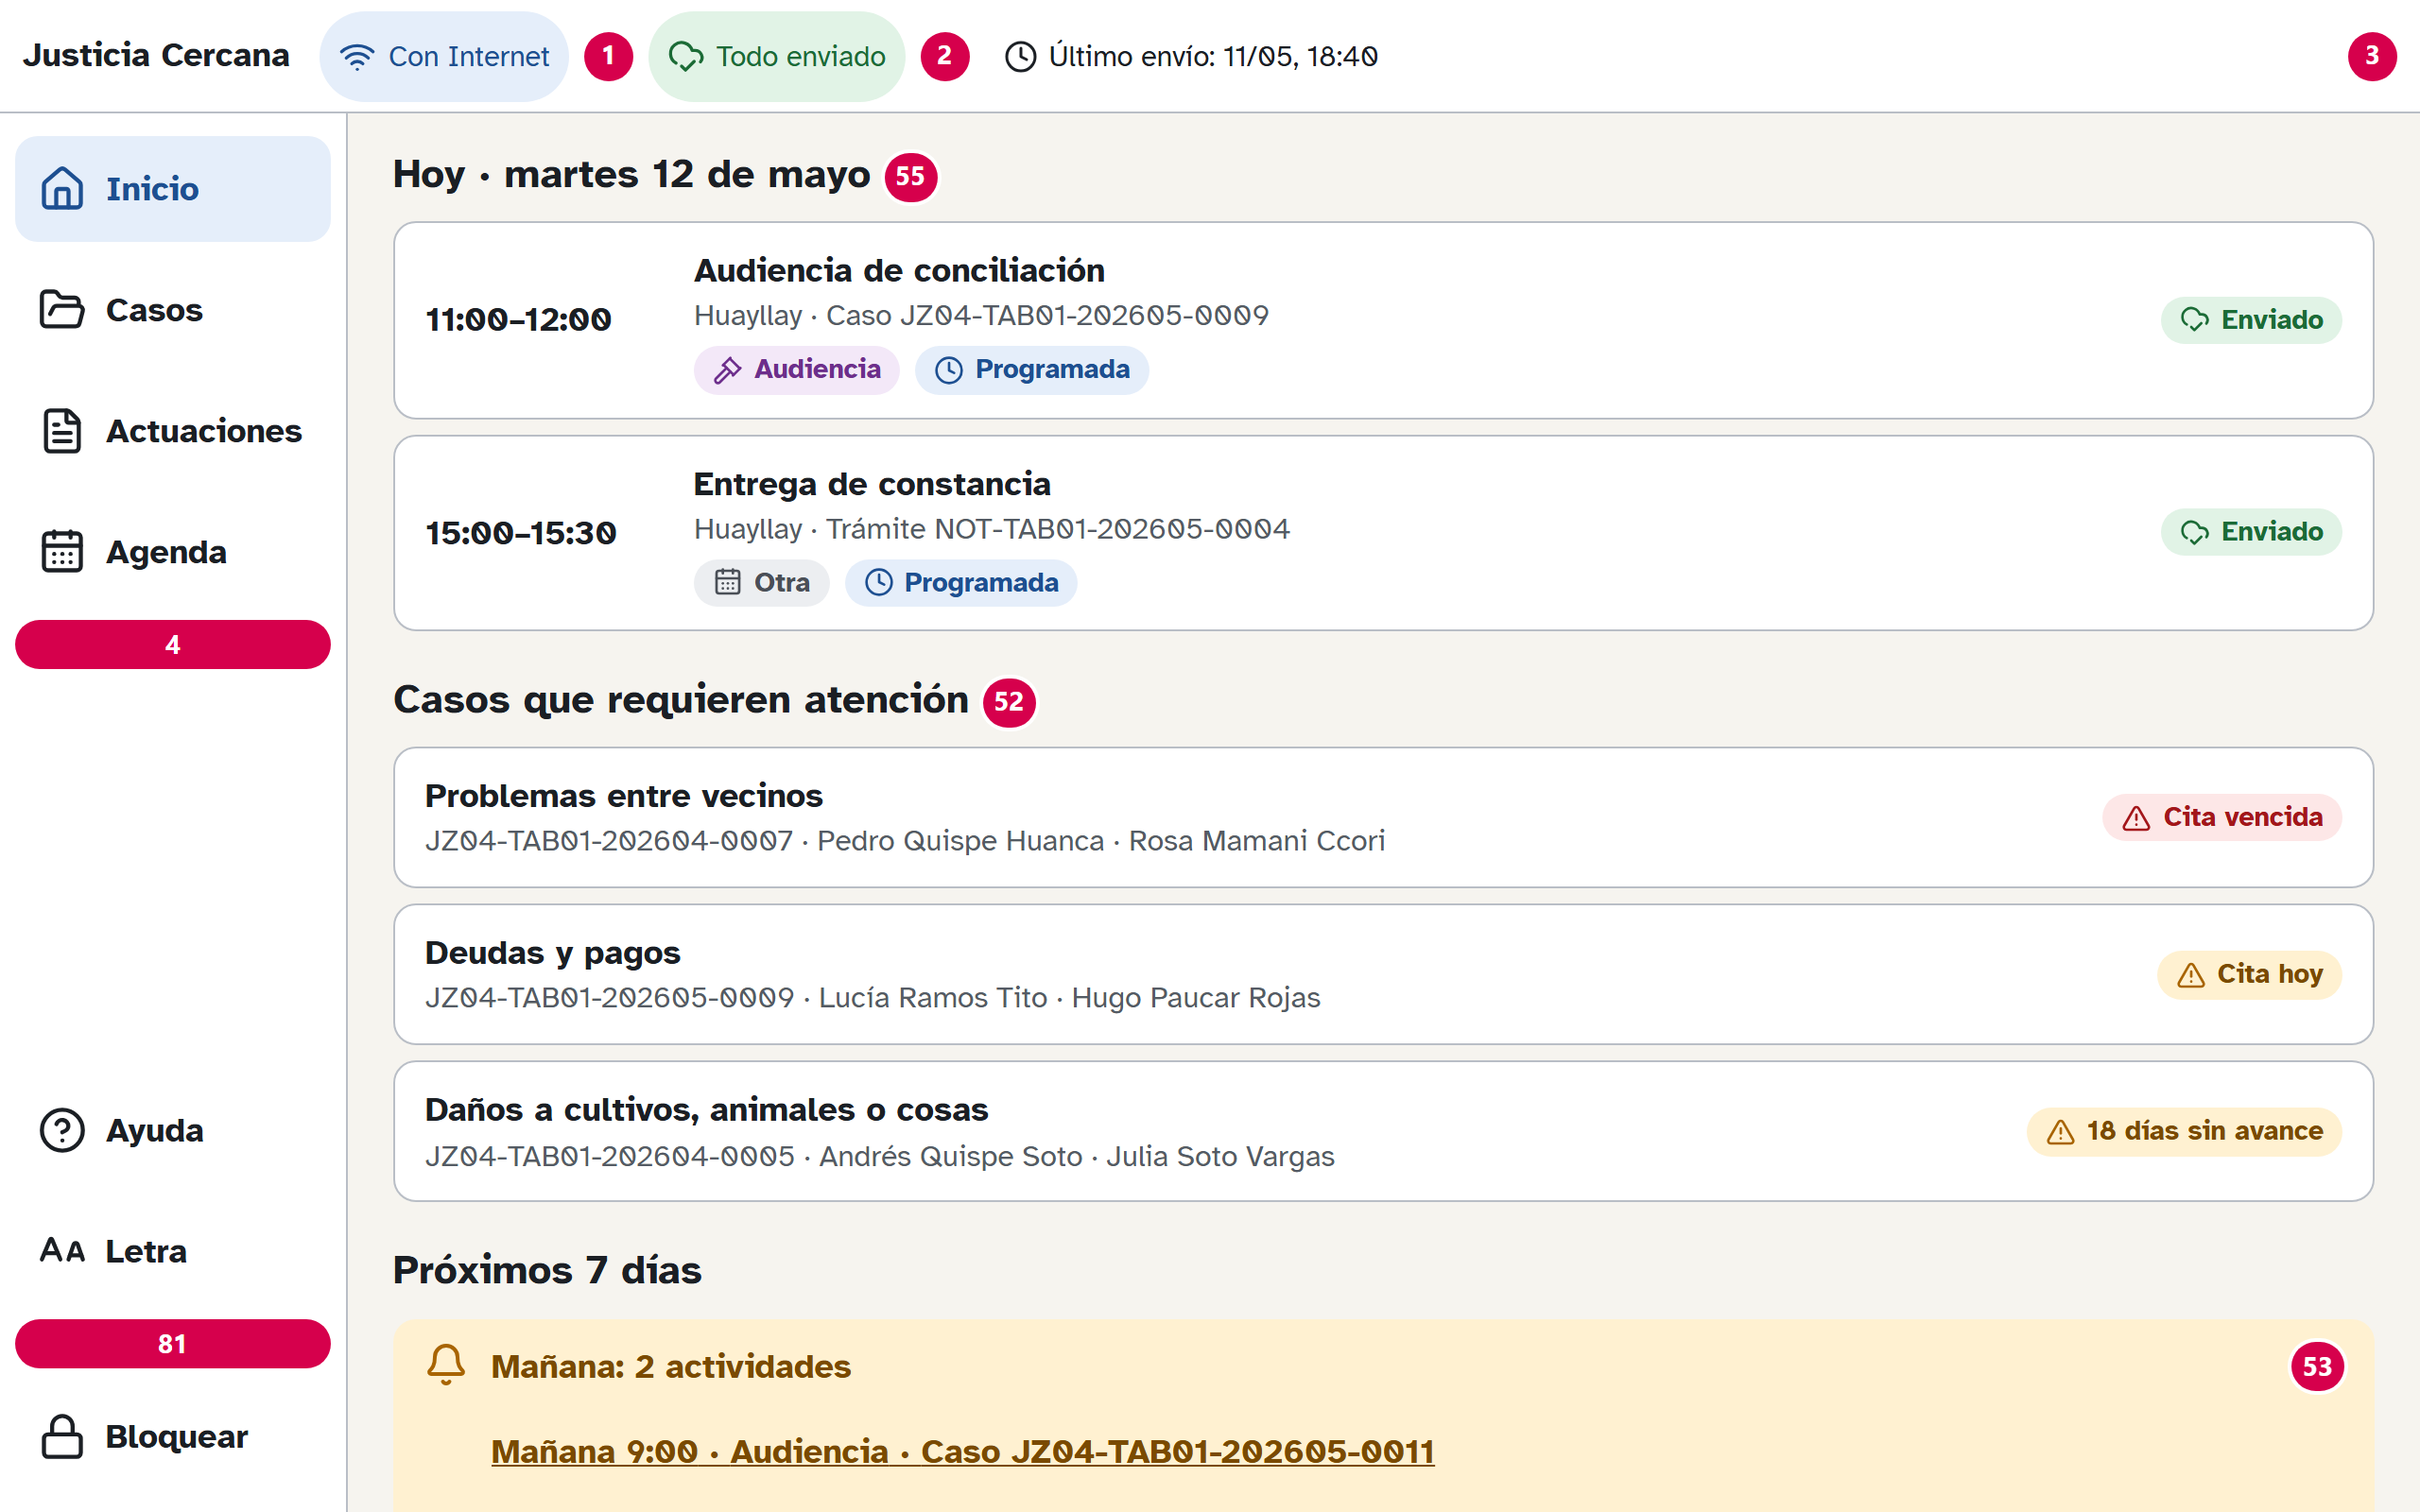
\includegraphics[width=\linewidth]{../../captures/ANOT_P-01_inicio.png}\\[-2pt]{\footnotesize\raggedright\textbf{P-01.} Marcadores numerados = IDs de la matriz de justificación \emph{(Justificación de las decisiones)}\par}\end{minipage}\hfill
\begin{minipage}[t]{0.49\textwidth}\centering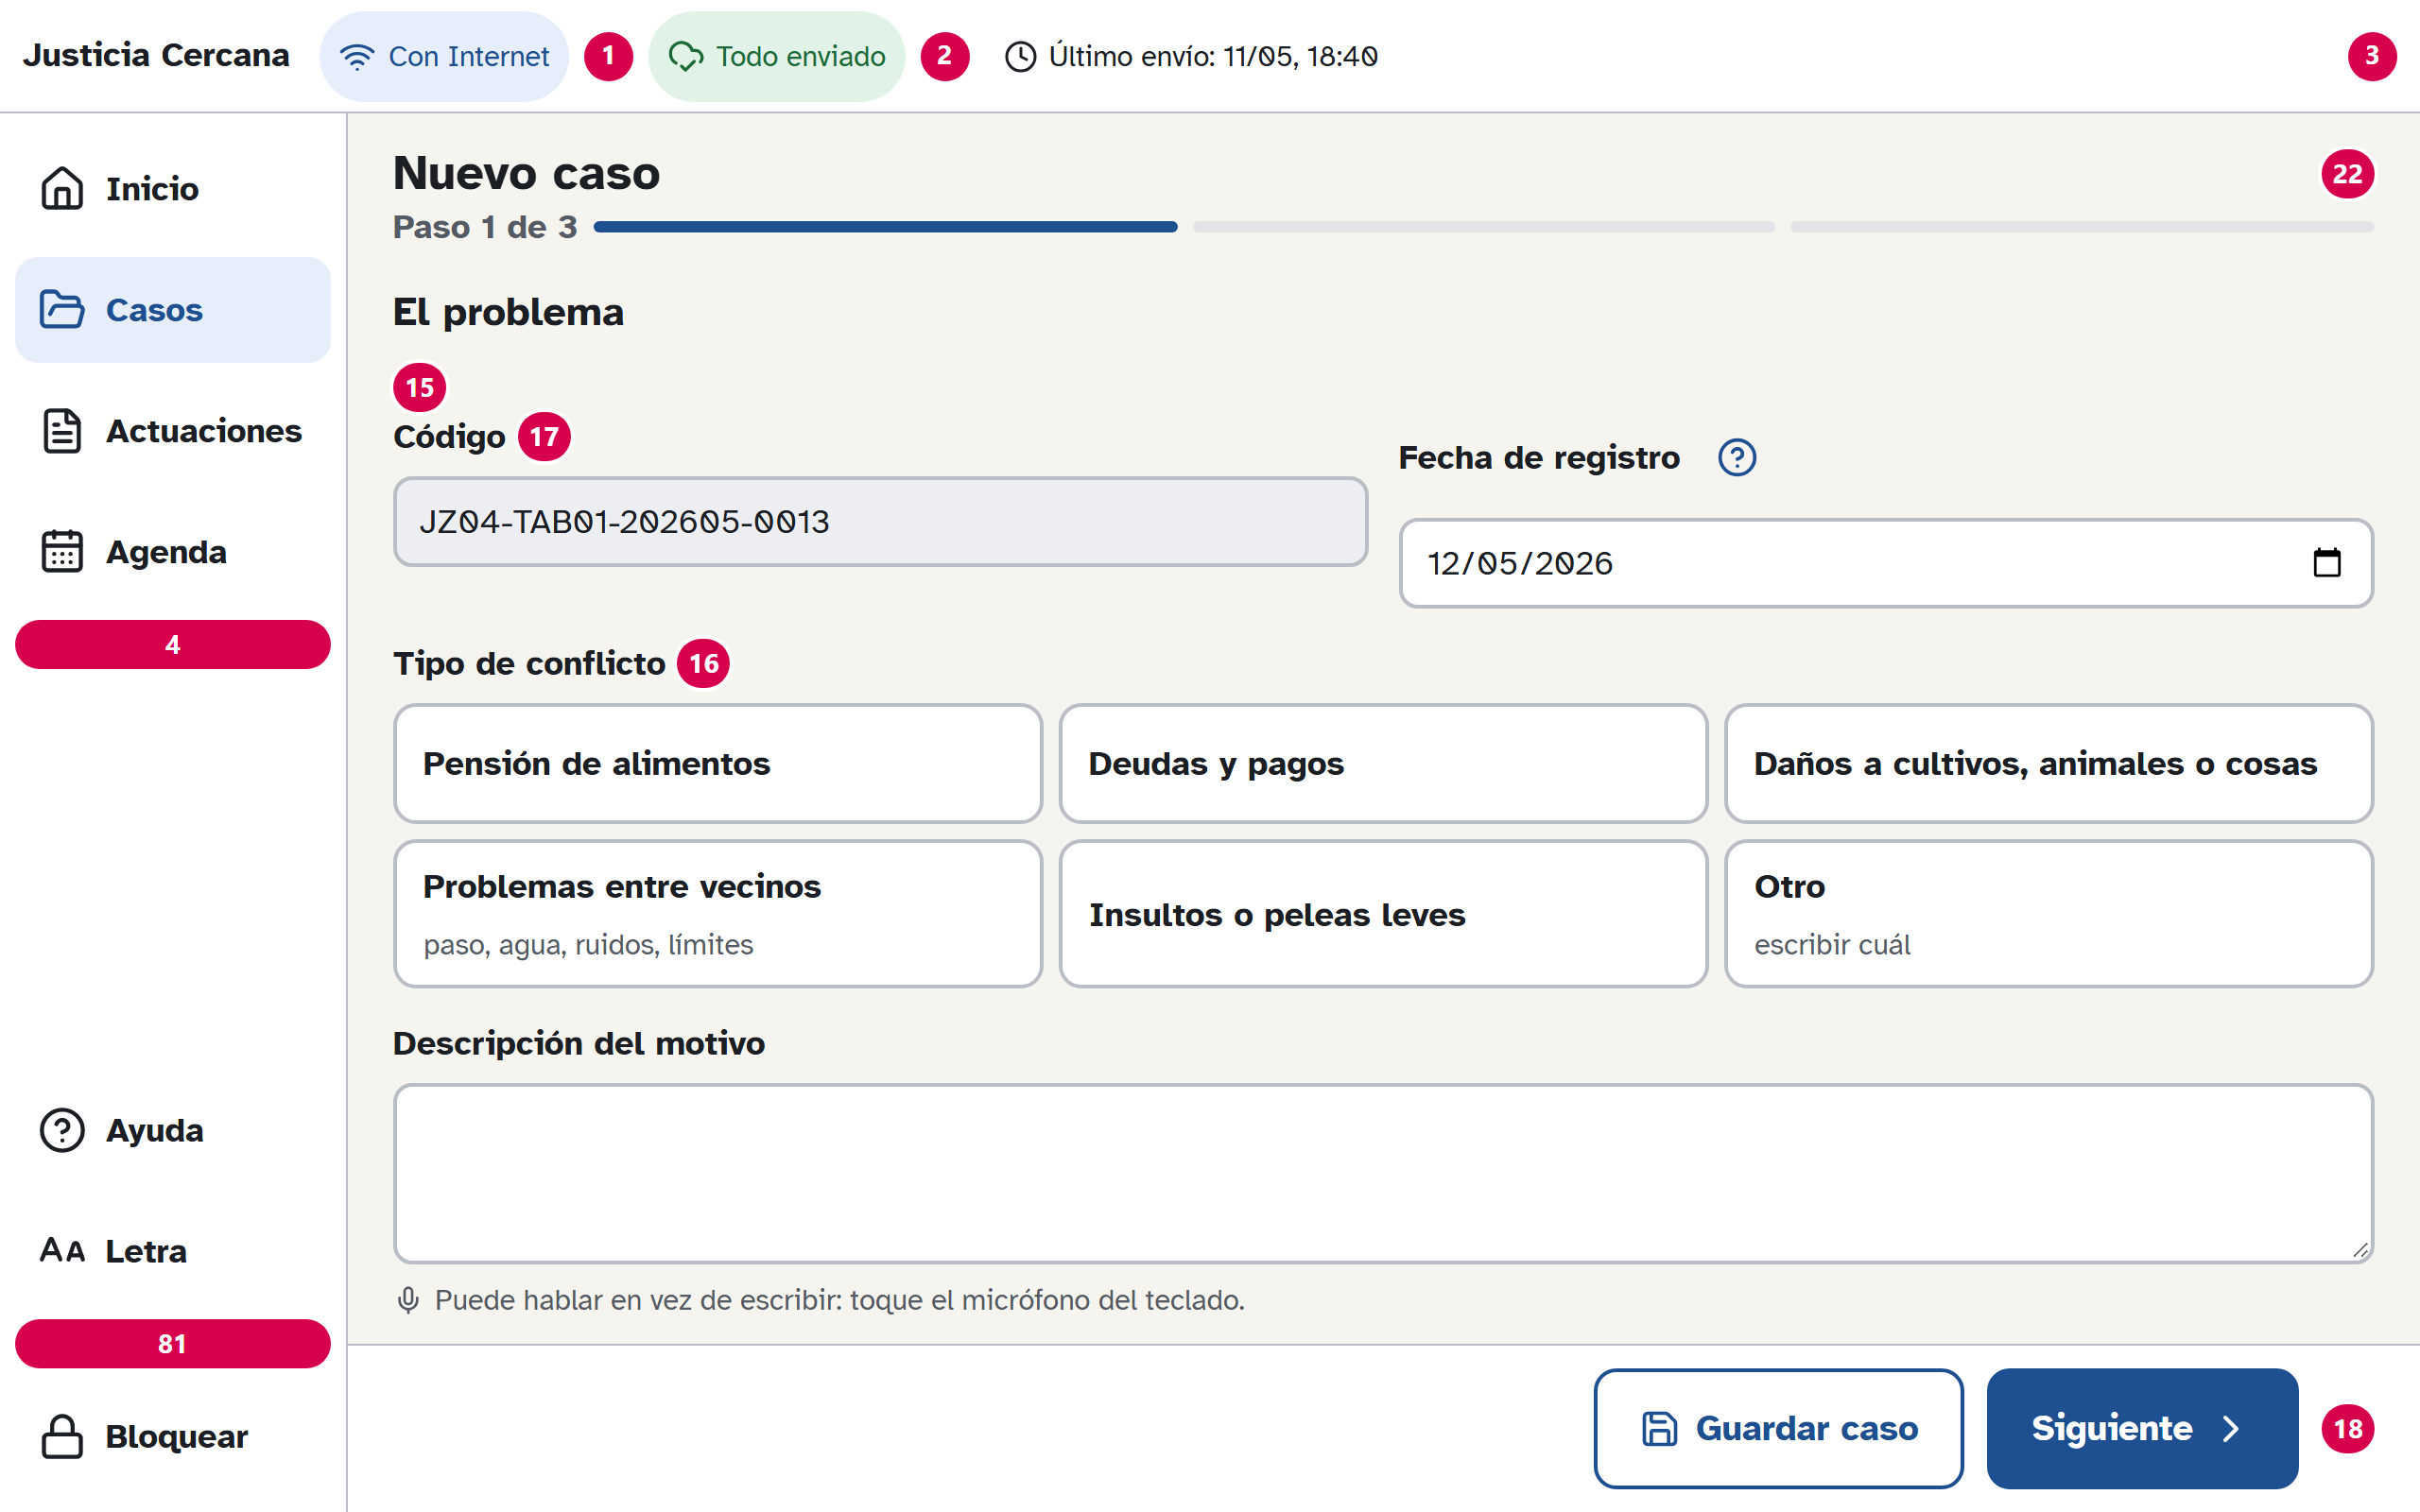
\includegraphics[width=\linewidth]{../../captures/ANOT_P-03_caso-nuevo.png}\\[-2pt]{\footnotesize\raggedright\textbf{P-03.} Marcadores numerados = IDs de la matriz de justificación \emph{(Justificación de las decisiones)}\par}\end{minipage}\par\vspace{8pt}\noindent
\begin{minipage}[t]{0.49\textwidth}\centering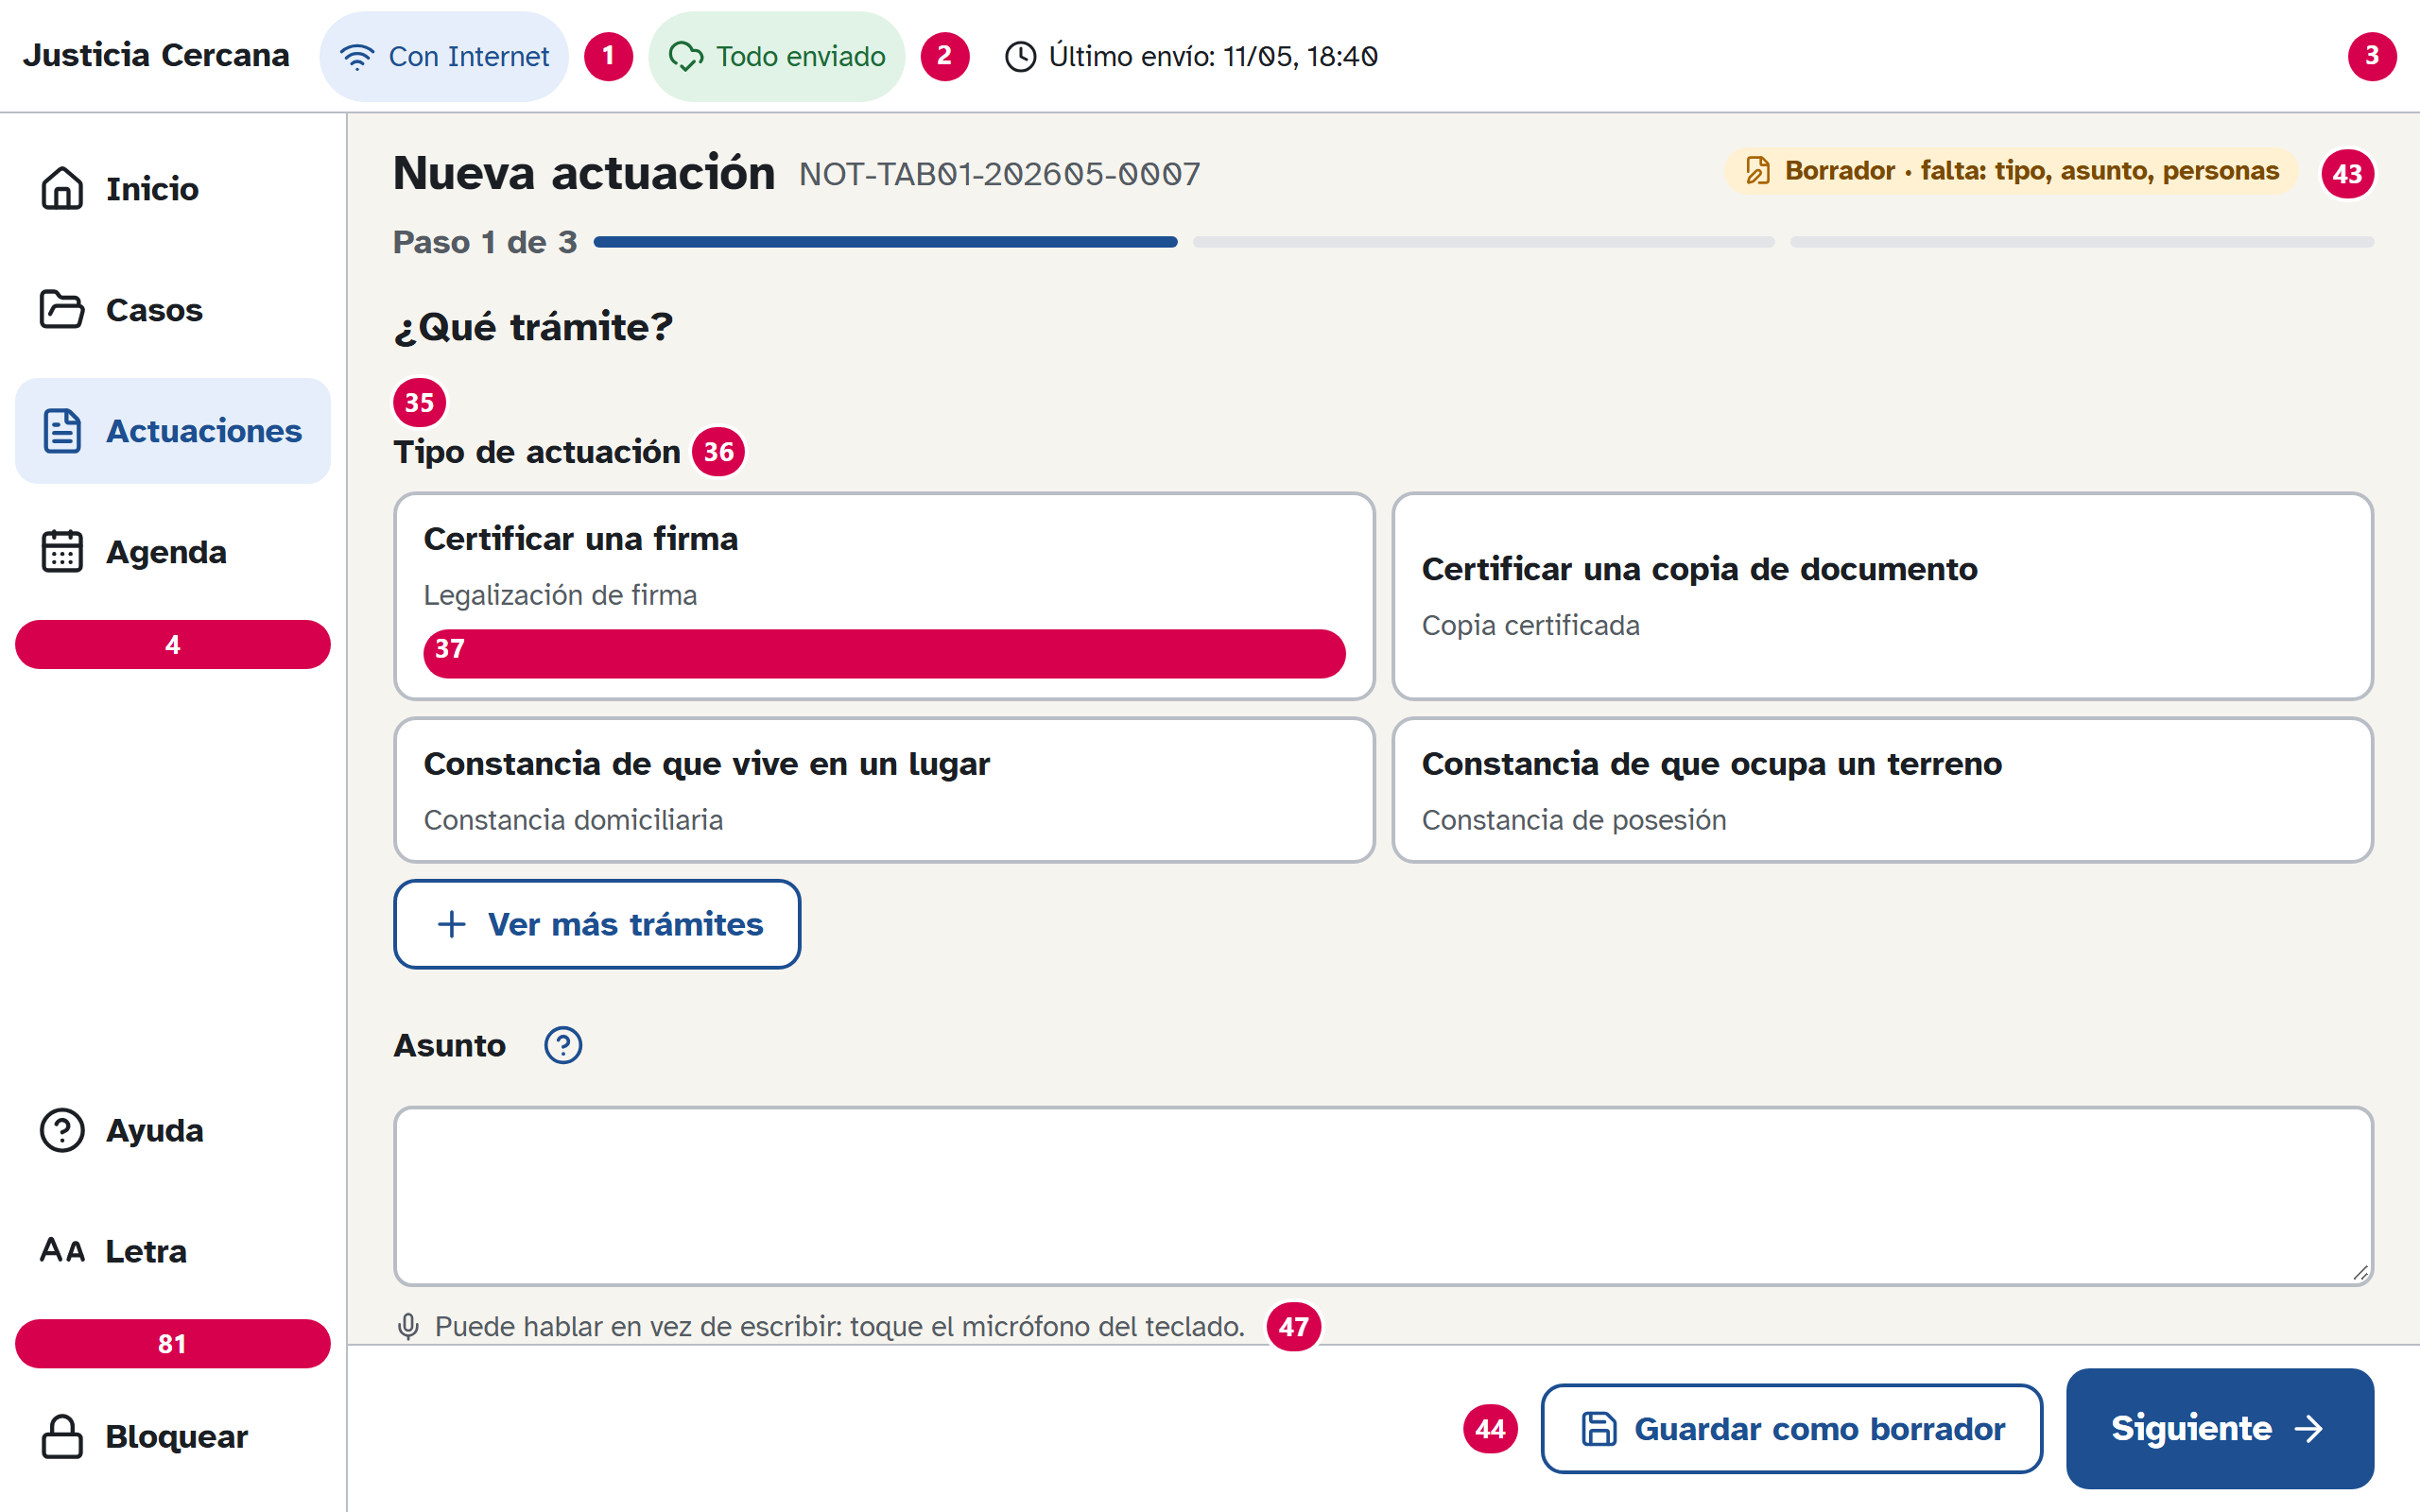
\includegraphics[width=\linewidth]{../../captures/ANOT_P-06_actuacion-nueva.png}\\[-2pt]{\footnotesize\raggedright\textbf{P-06.} Marcadores numerados = IDs de la matriz de justificación \emph{(Justificación de las decisiones)}\par}\end{minipage}\hfill
\begin{minipage}[t]{0.49\textwidth}\centering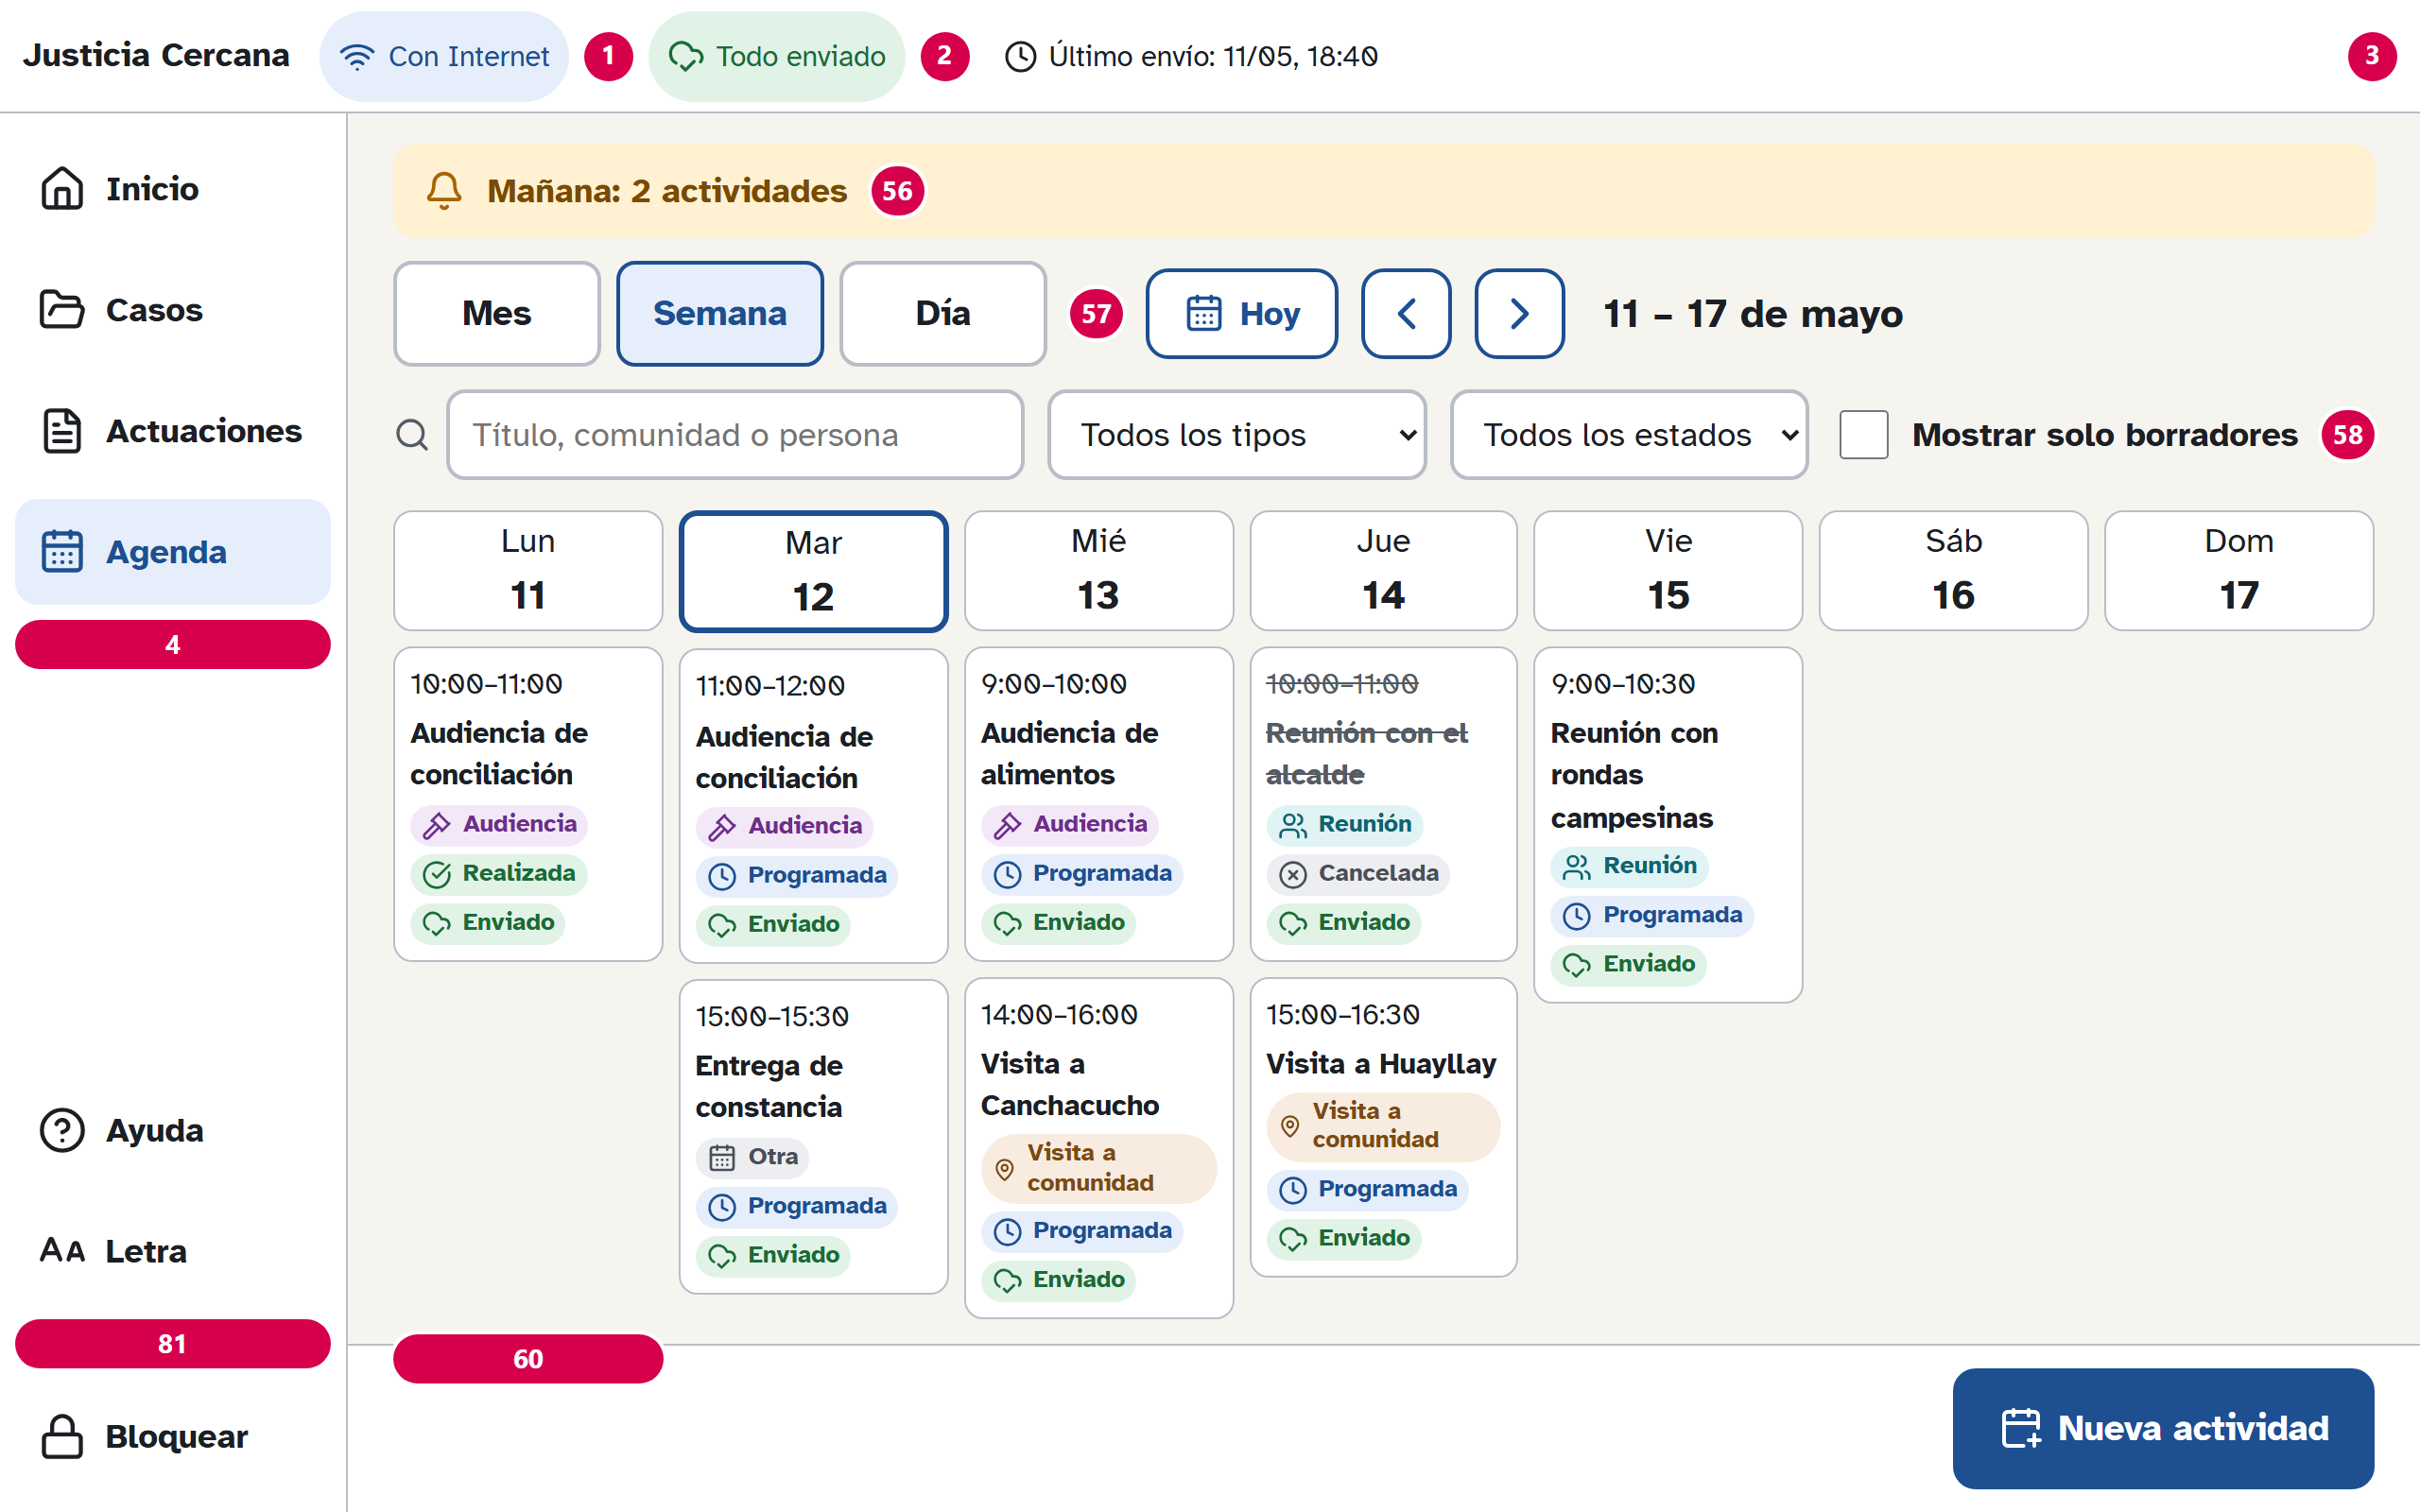
\includegraphics[width=\linewidth]{../../captures/ANOT_P-07_agenda.png}\\[-2pt]{\footnotesize\raggedright\textbf{P-07.} Marcadores numerados = IDs de la matriz de justificación \emph{(Justificación de las decisiones)}\par}\end{minipage}\par\vspace{8pt}\noindent
\begin{minipage}[t]{0.49\textwidth}\centering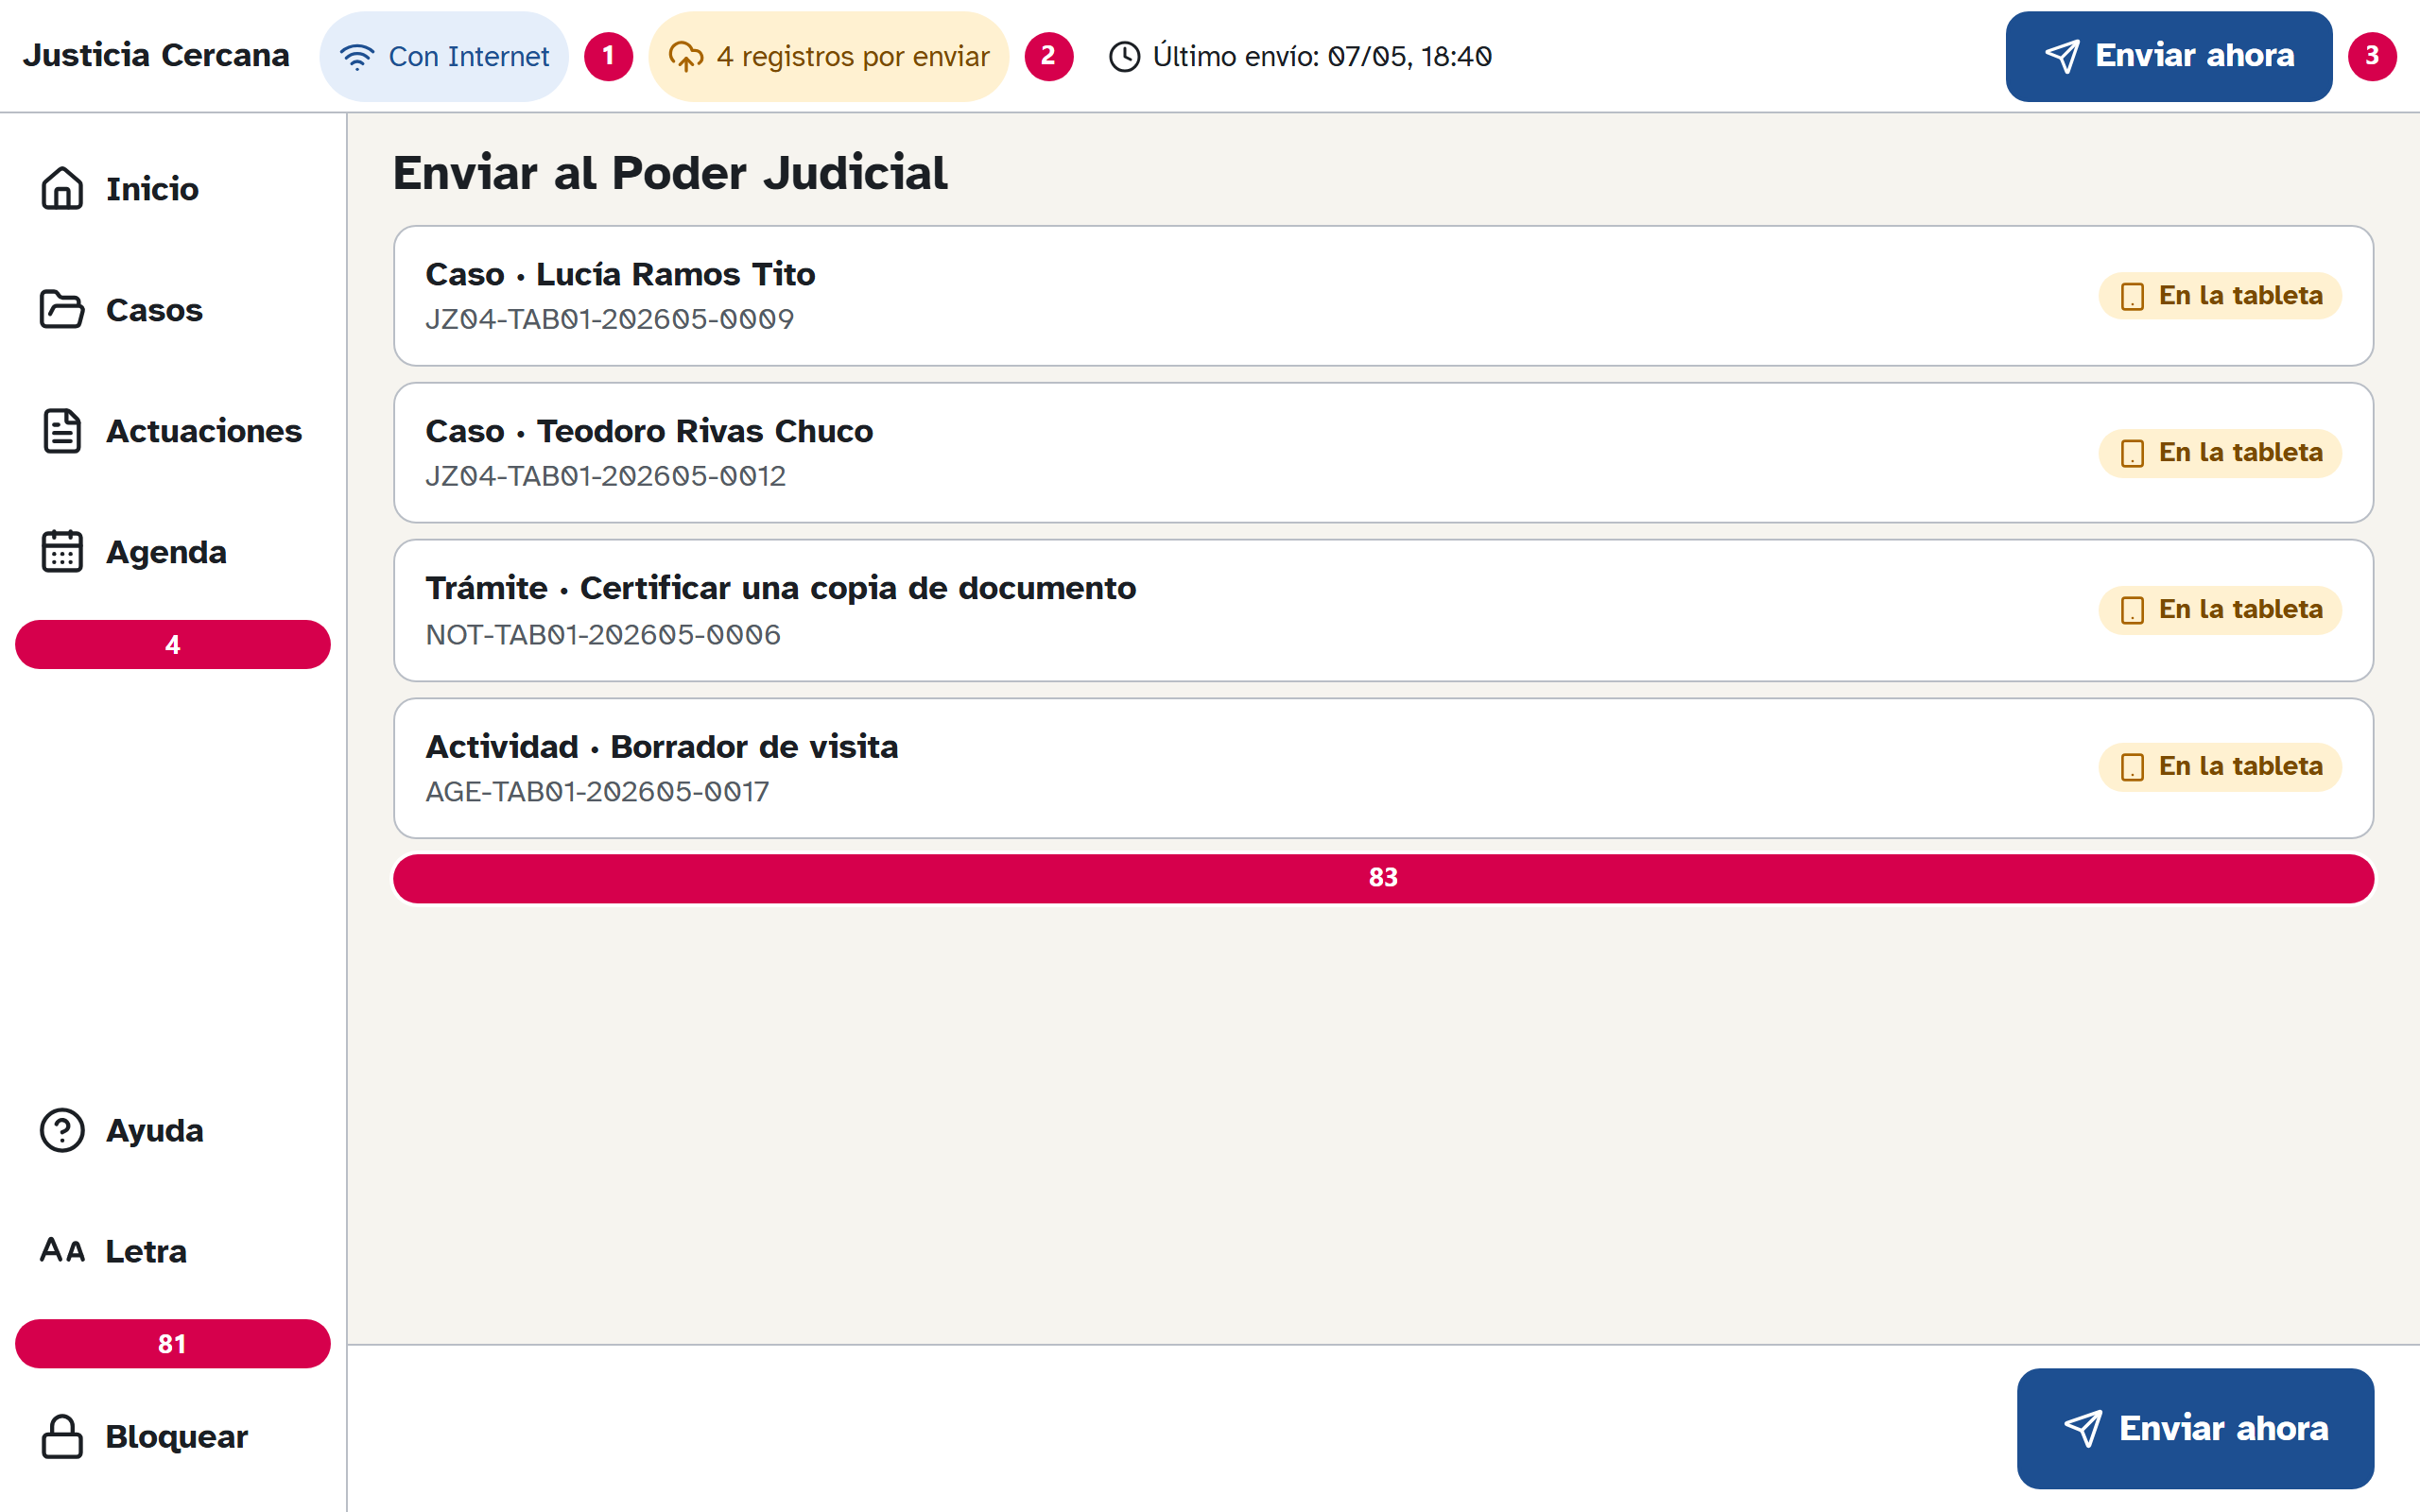
\includegraphics[width=\linewidth]{../../captures/ANOT_P-09_envio.png}\\[-2pt]{\footnotesize\raggedright\textbf{P-09.} Marcadores numerados = IDs de la matriz de justificación \emph{(Justificación de las decisiones)}\par}\end{minipage}\hfill
\begin{minipage}[t]{0.49\textwidth}\centering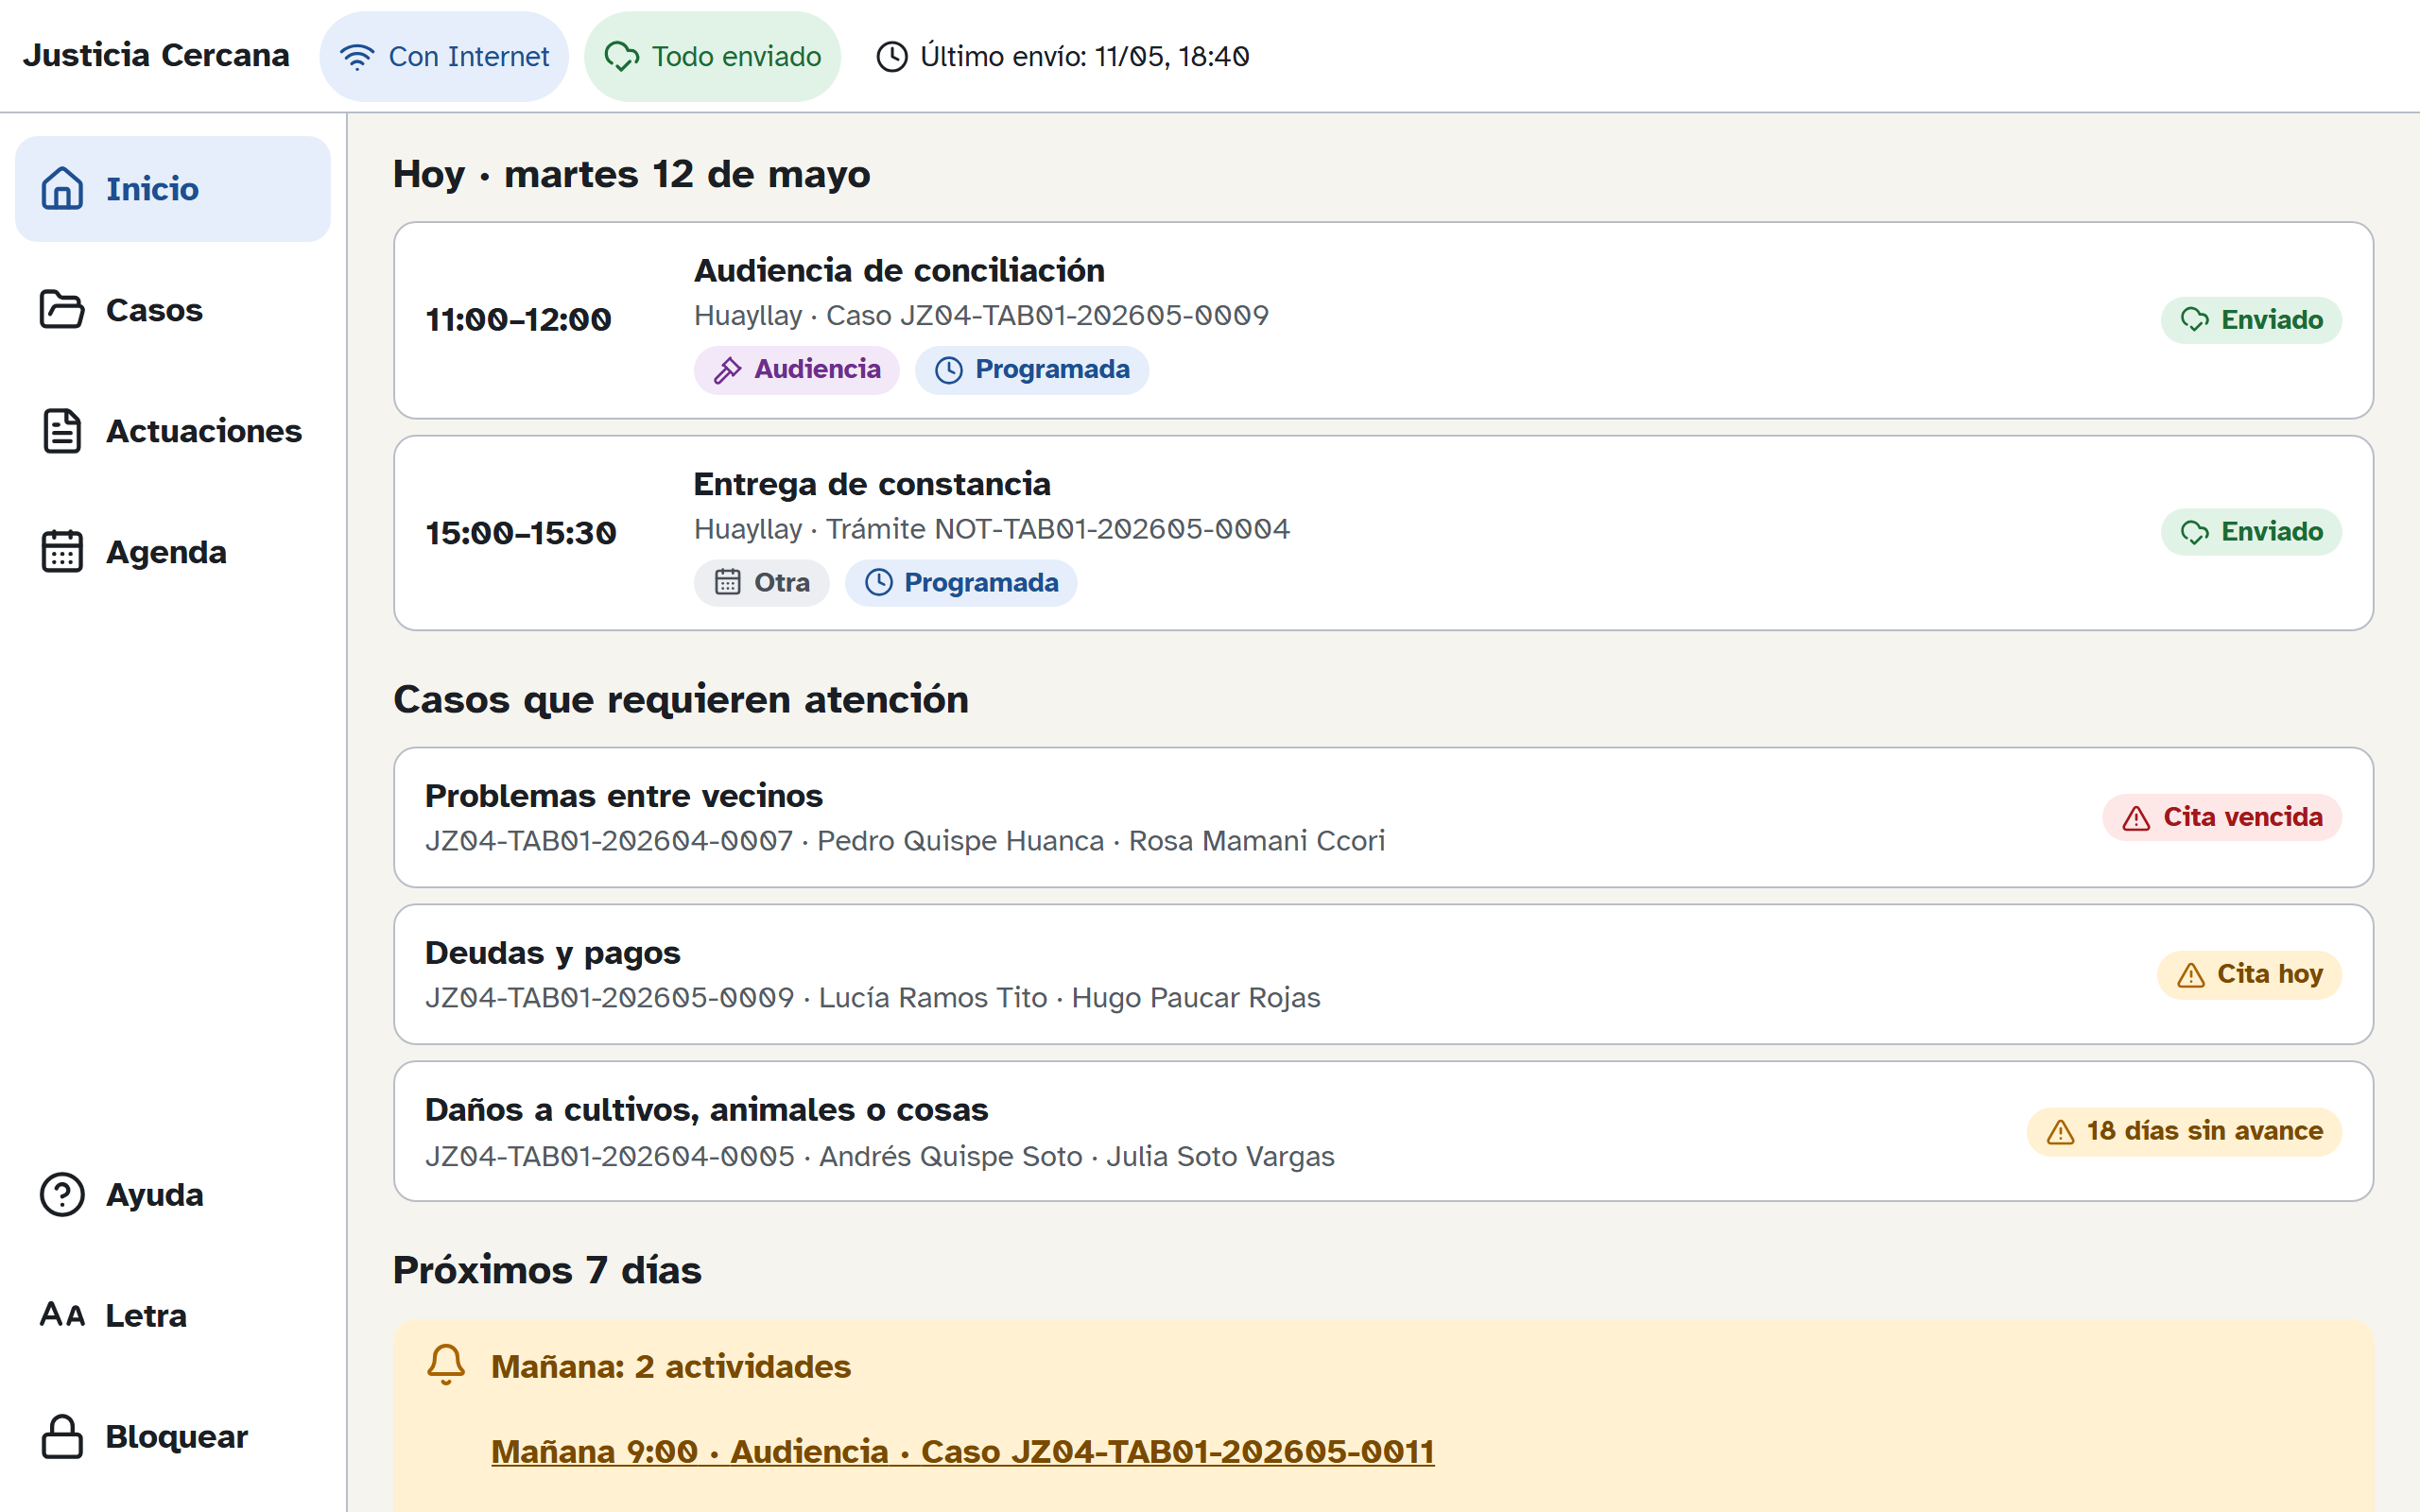
\includegraphics[width=\linewidth]{../../captures/G-01_barra-con-internet-todo-enviado.png}\\[-2pt]{\footnotesize\raggedright\textbf{Barra.} ``Con Internet'' (azul) · ``Todo enviado'' (verde) · último envío \emph{(Funcionamiento sin conexión)}\par}\end{minipage}\par\vspace{8pt}\noindent
\begin{minipage}[t]{0.49\textwidth}\centering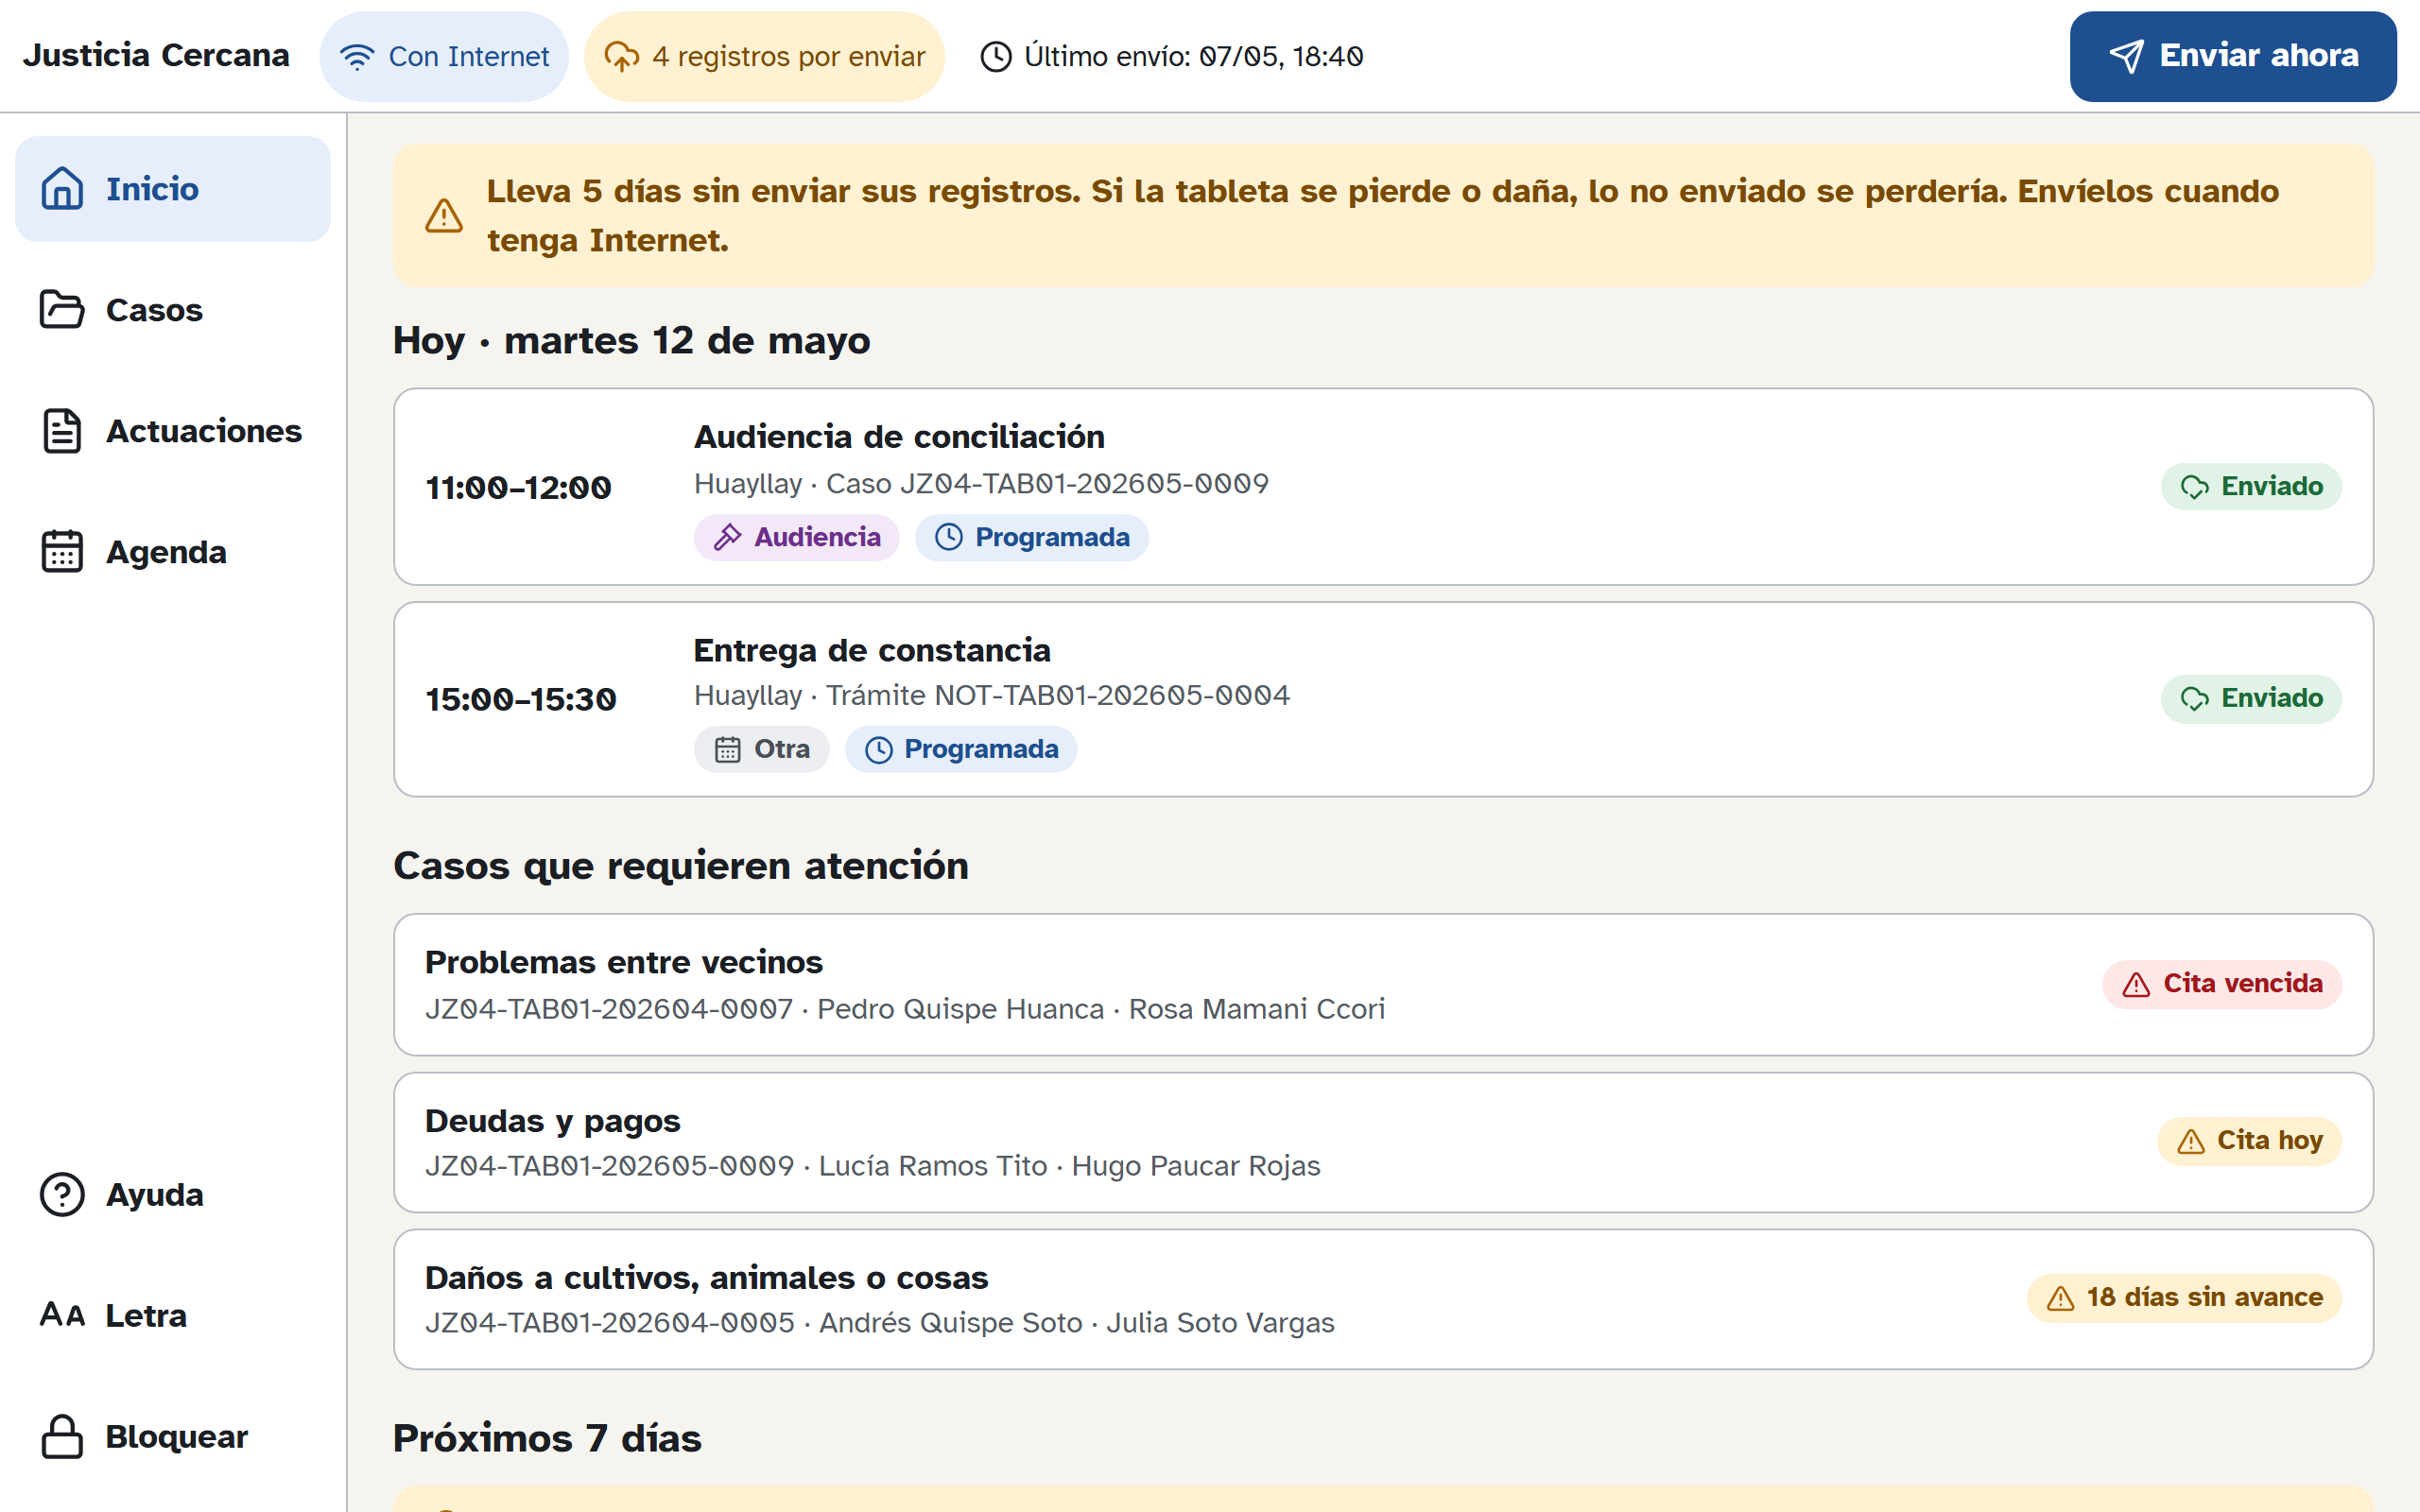
\includegraphics[width=\linewidth]{../../captures/G-02_barra-con-internet-pendientes-enviar-ahora.png}\\[-2pt]{\footnotesize\raggedright\textbf{Barra.} ``4 registros por enviar'' (ámbar) y botón visible [Enviar ahora] \emph{(Funcionamiento sin conexión)}\par}\end{minipage}\hfill
\begin{minipage}[t]{0.49\textwidth}\centering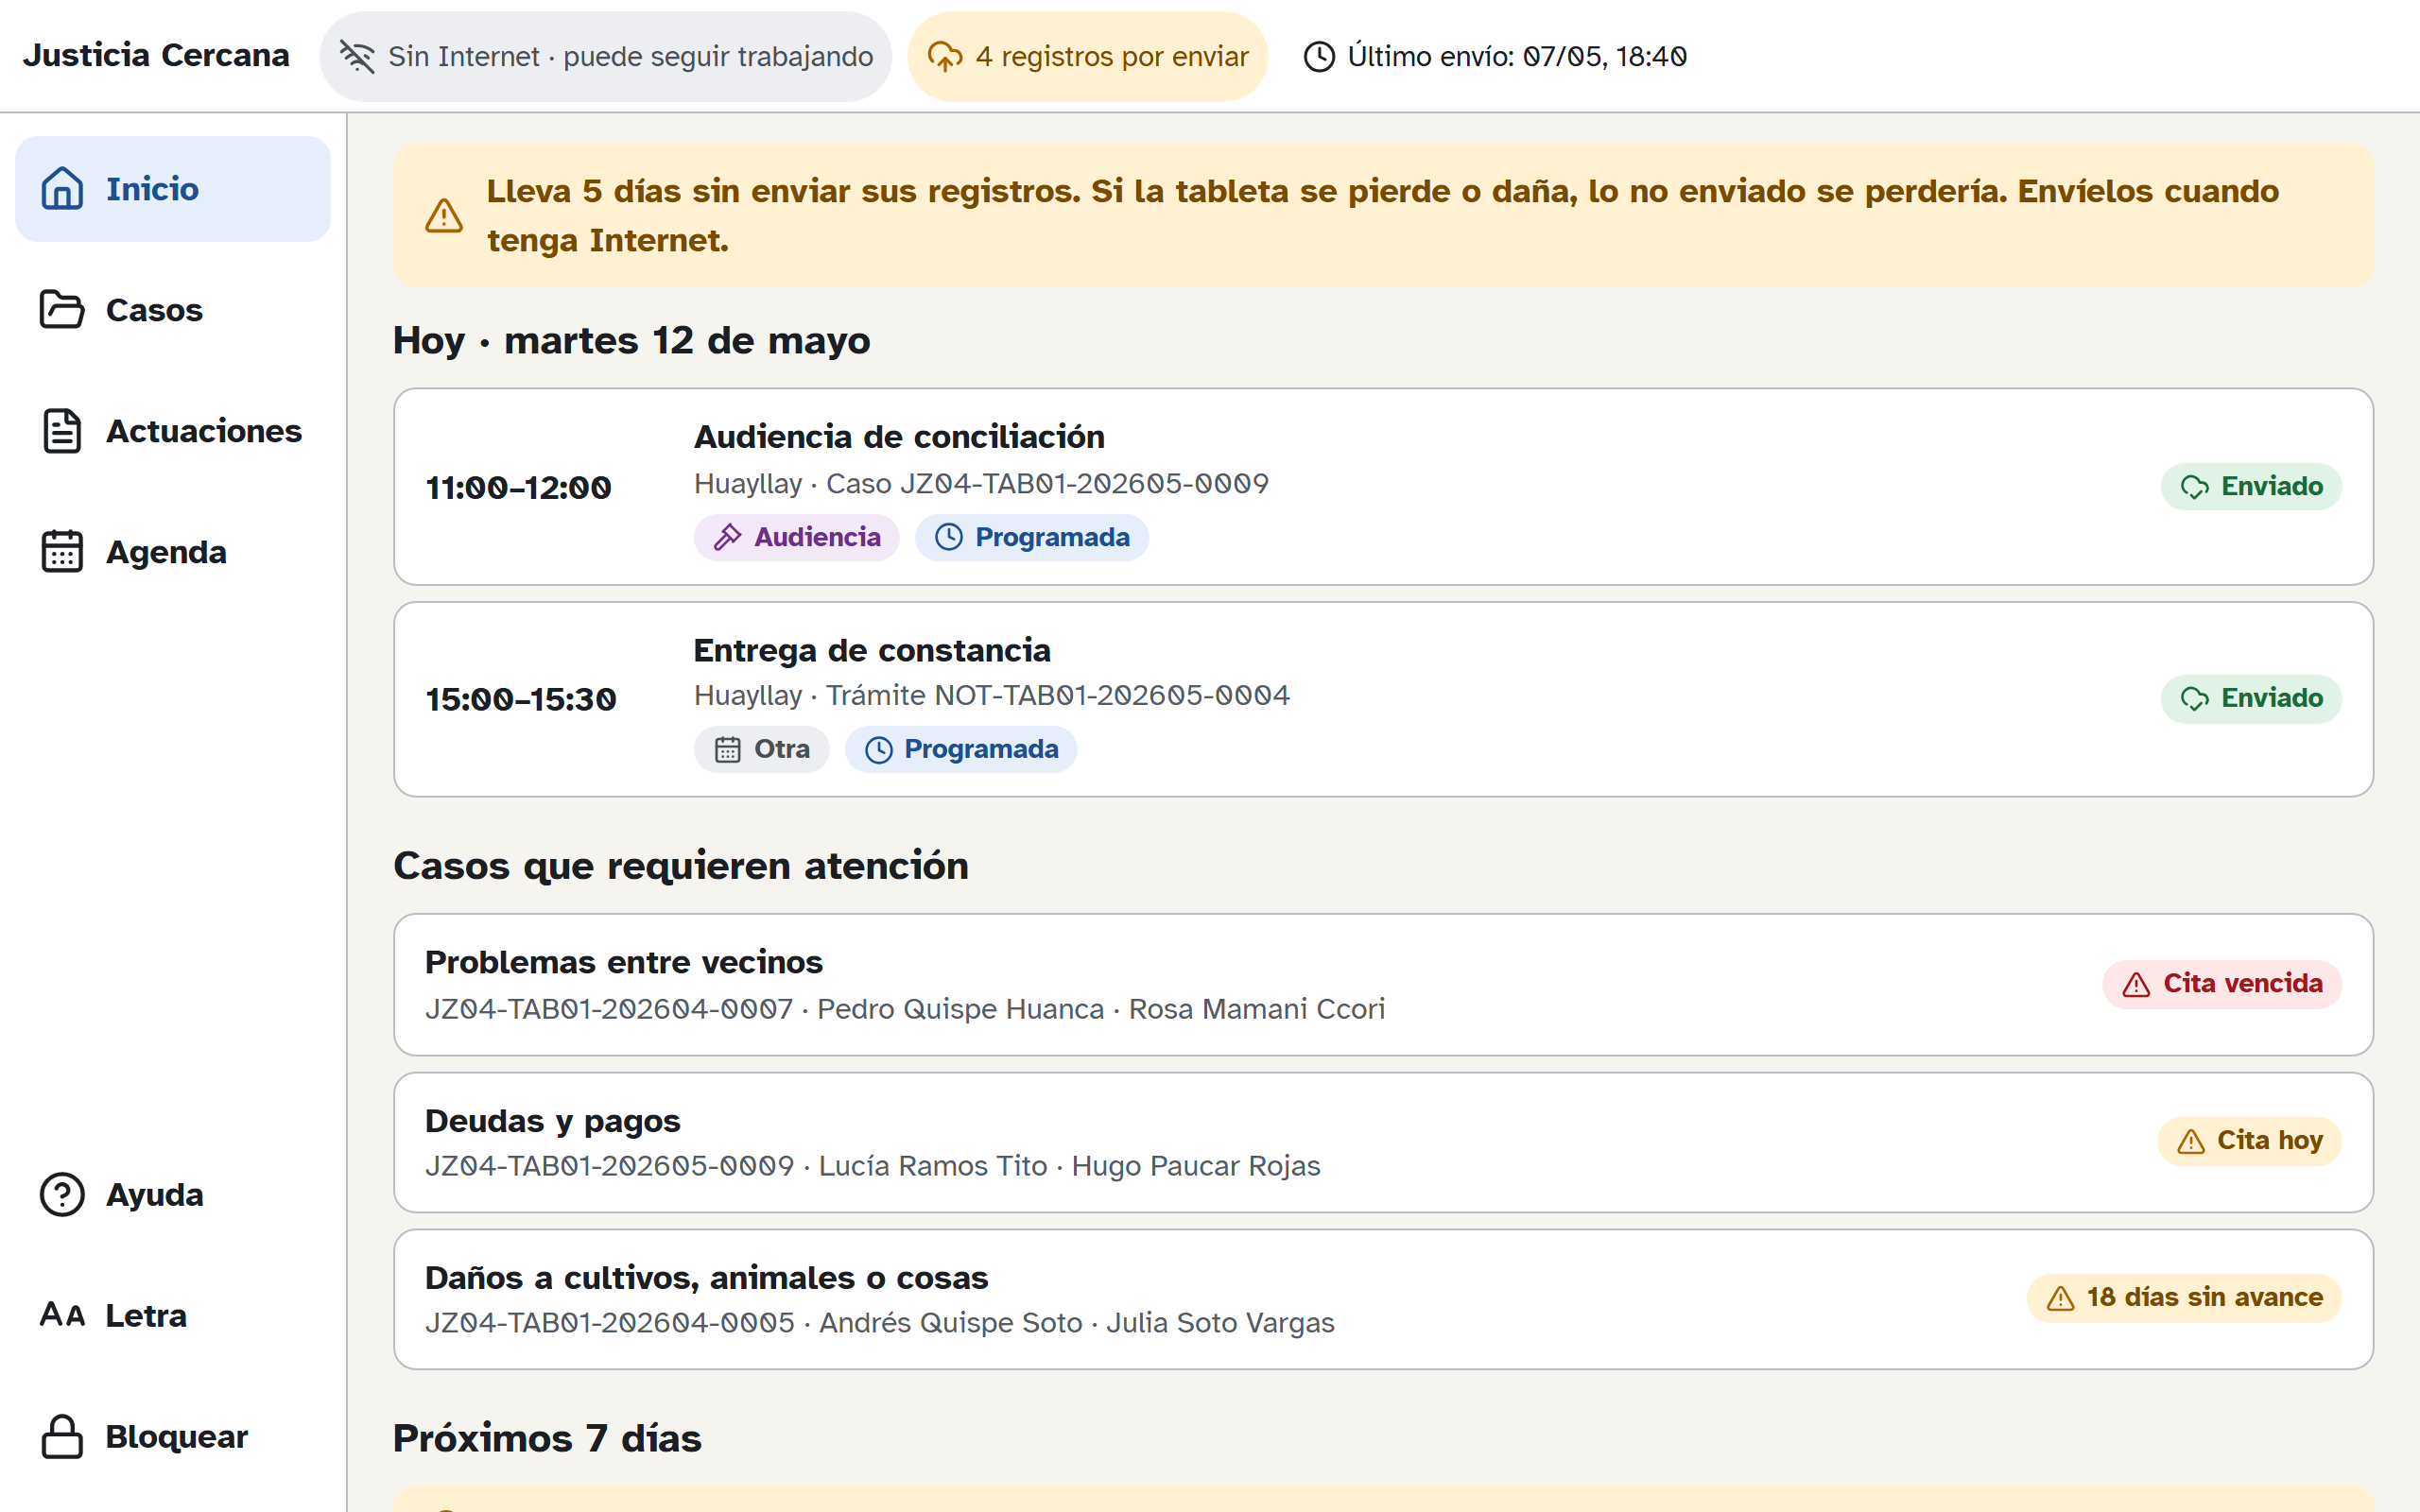
\includegraphics[width=\linewidth]{../../captures/G-03_barra-sin-internet-pendientes.png}\\[-2pt]{\footnotesize\raggedright\textbf{Barra.} ``Sin Internet'' en gris (nunca rojo) · ``4 registros por enviar''; sin [Enviar ahora] \emph{(Funcionamiento sin conexión)}\par}\end{minipage}\par\vspace{8pt}\noindent
\begin{minipage}[t]{0.49\textwidth}\centering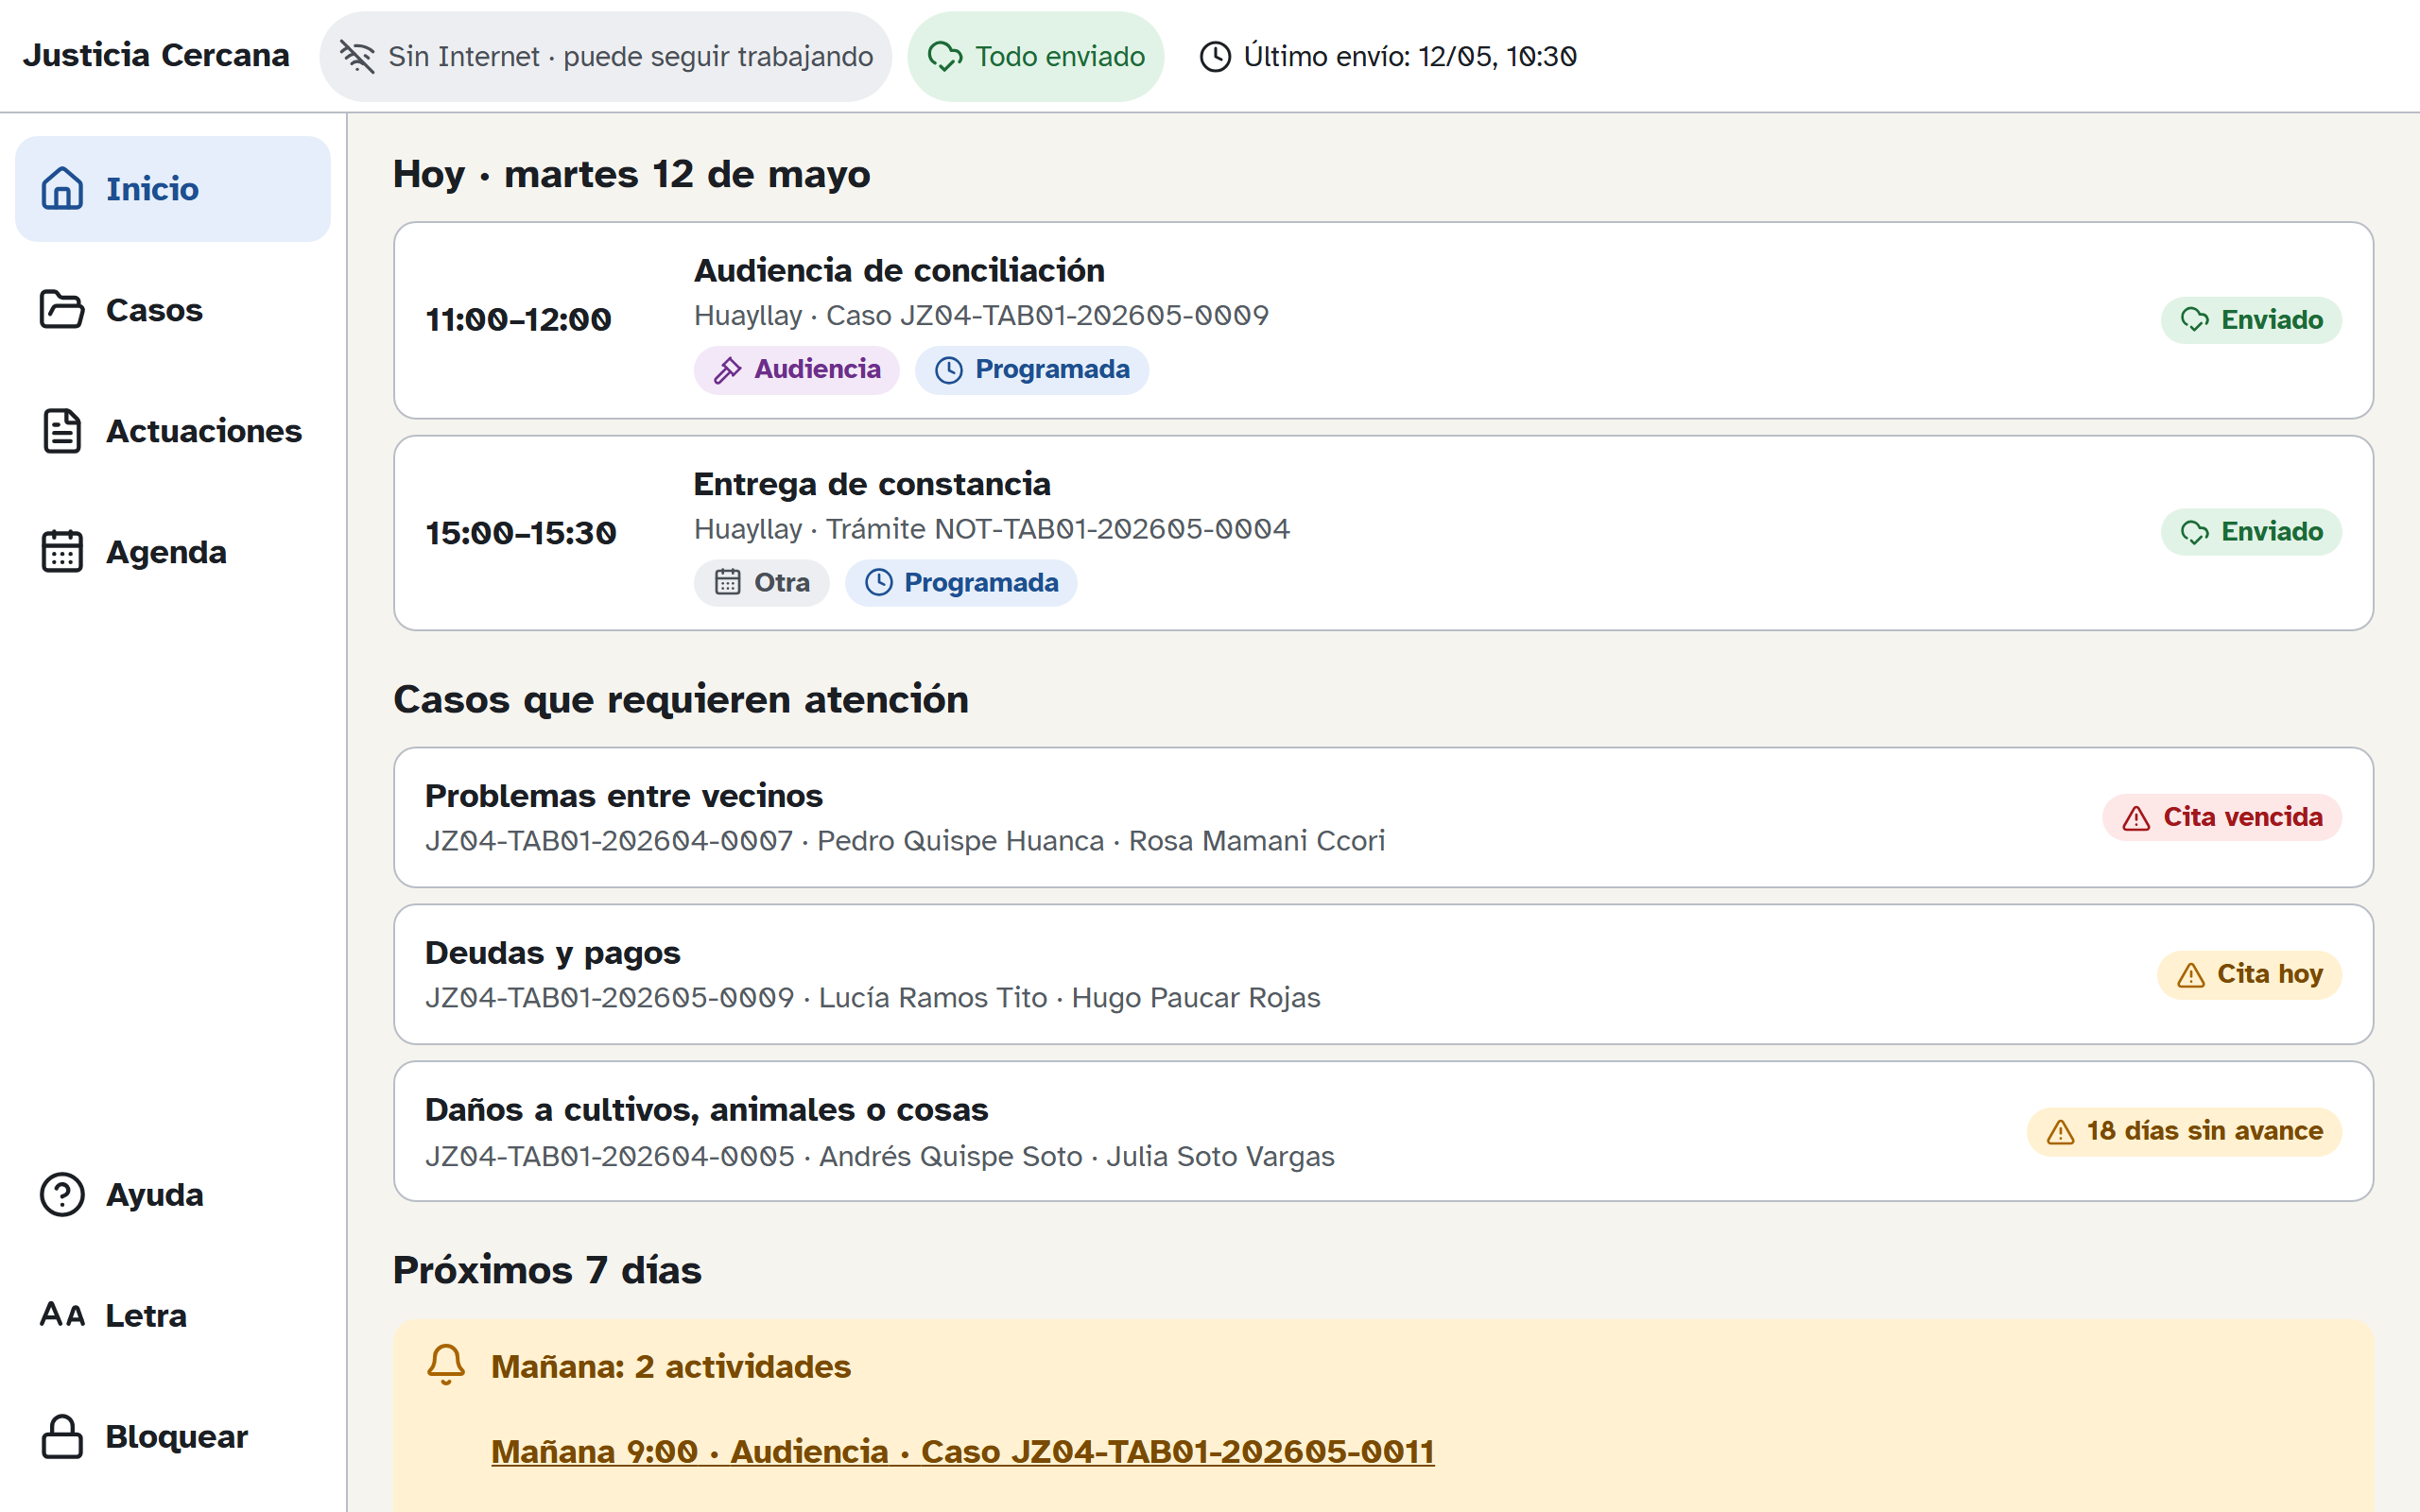
\includegraphics[width=\linewidth]{../../captures/G-04_barra-sin-internet-todo-enviado.png}\\[-2pt]{\footnotesize\raggedright\textbf{Barra.} ``Sin Internet'' (gris) · ``Todo enviado'' (verde) \emph{(Funcionamiento sin conexión)}\par}\end{minipage}\hfill
\begin{minipage}[t]{0.49\textwidth}\centering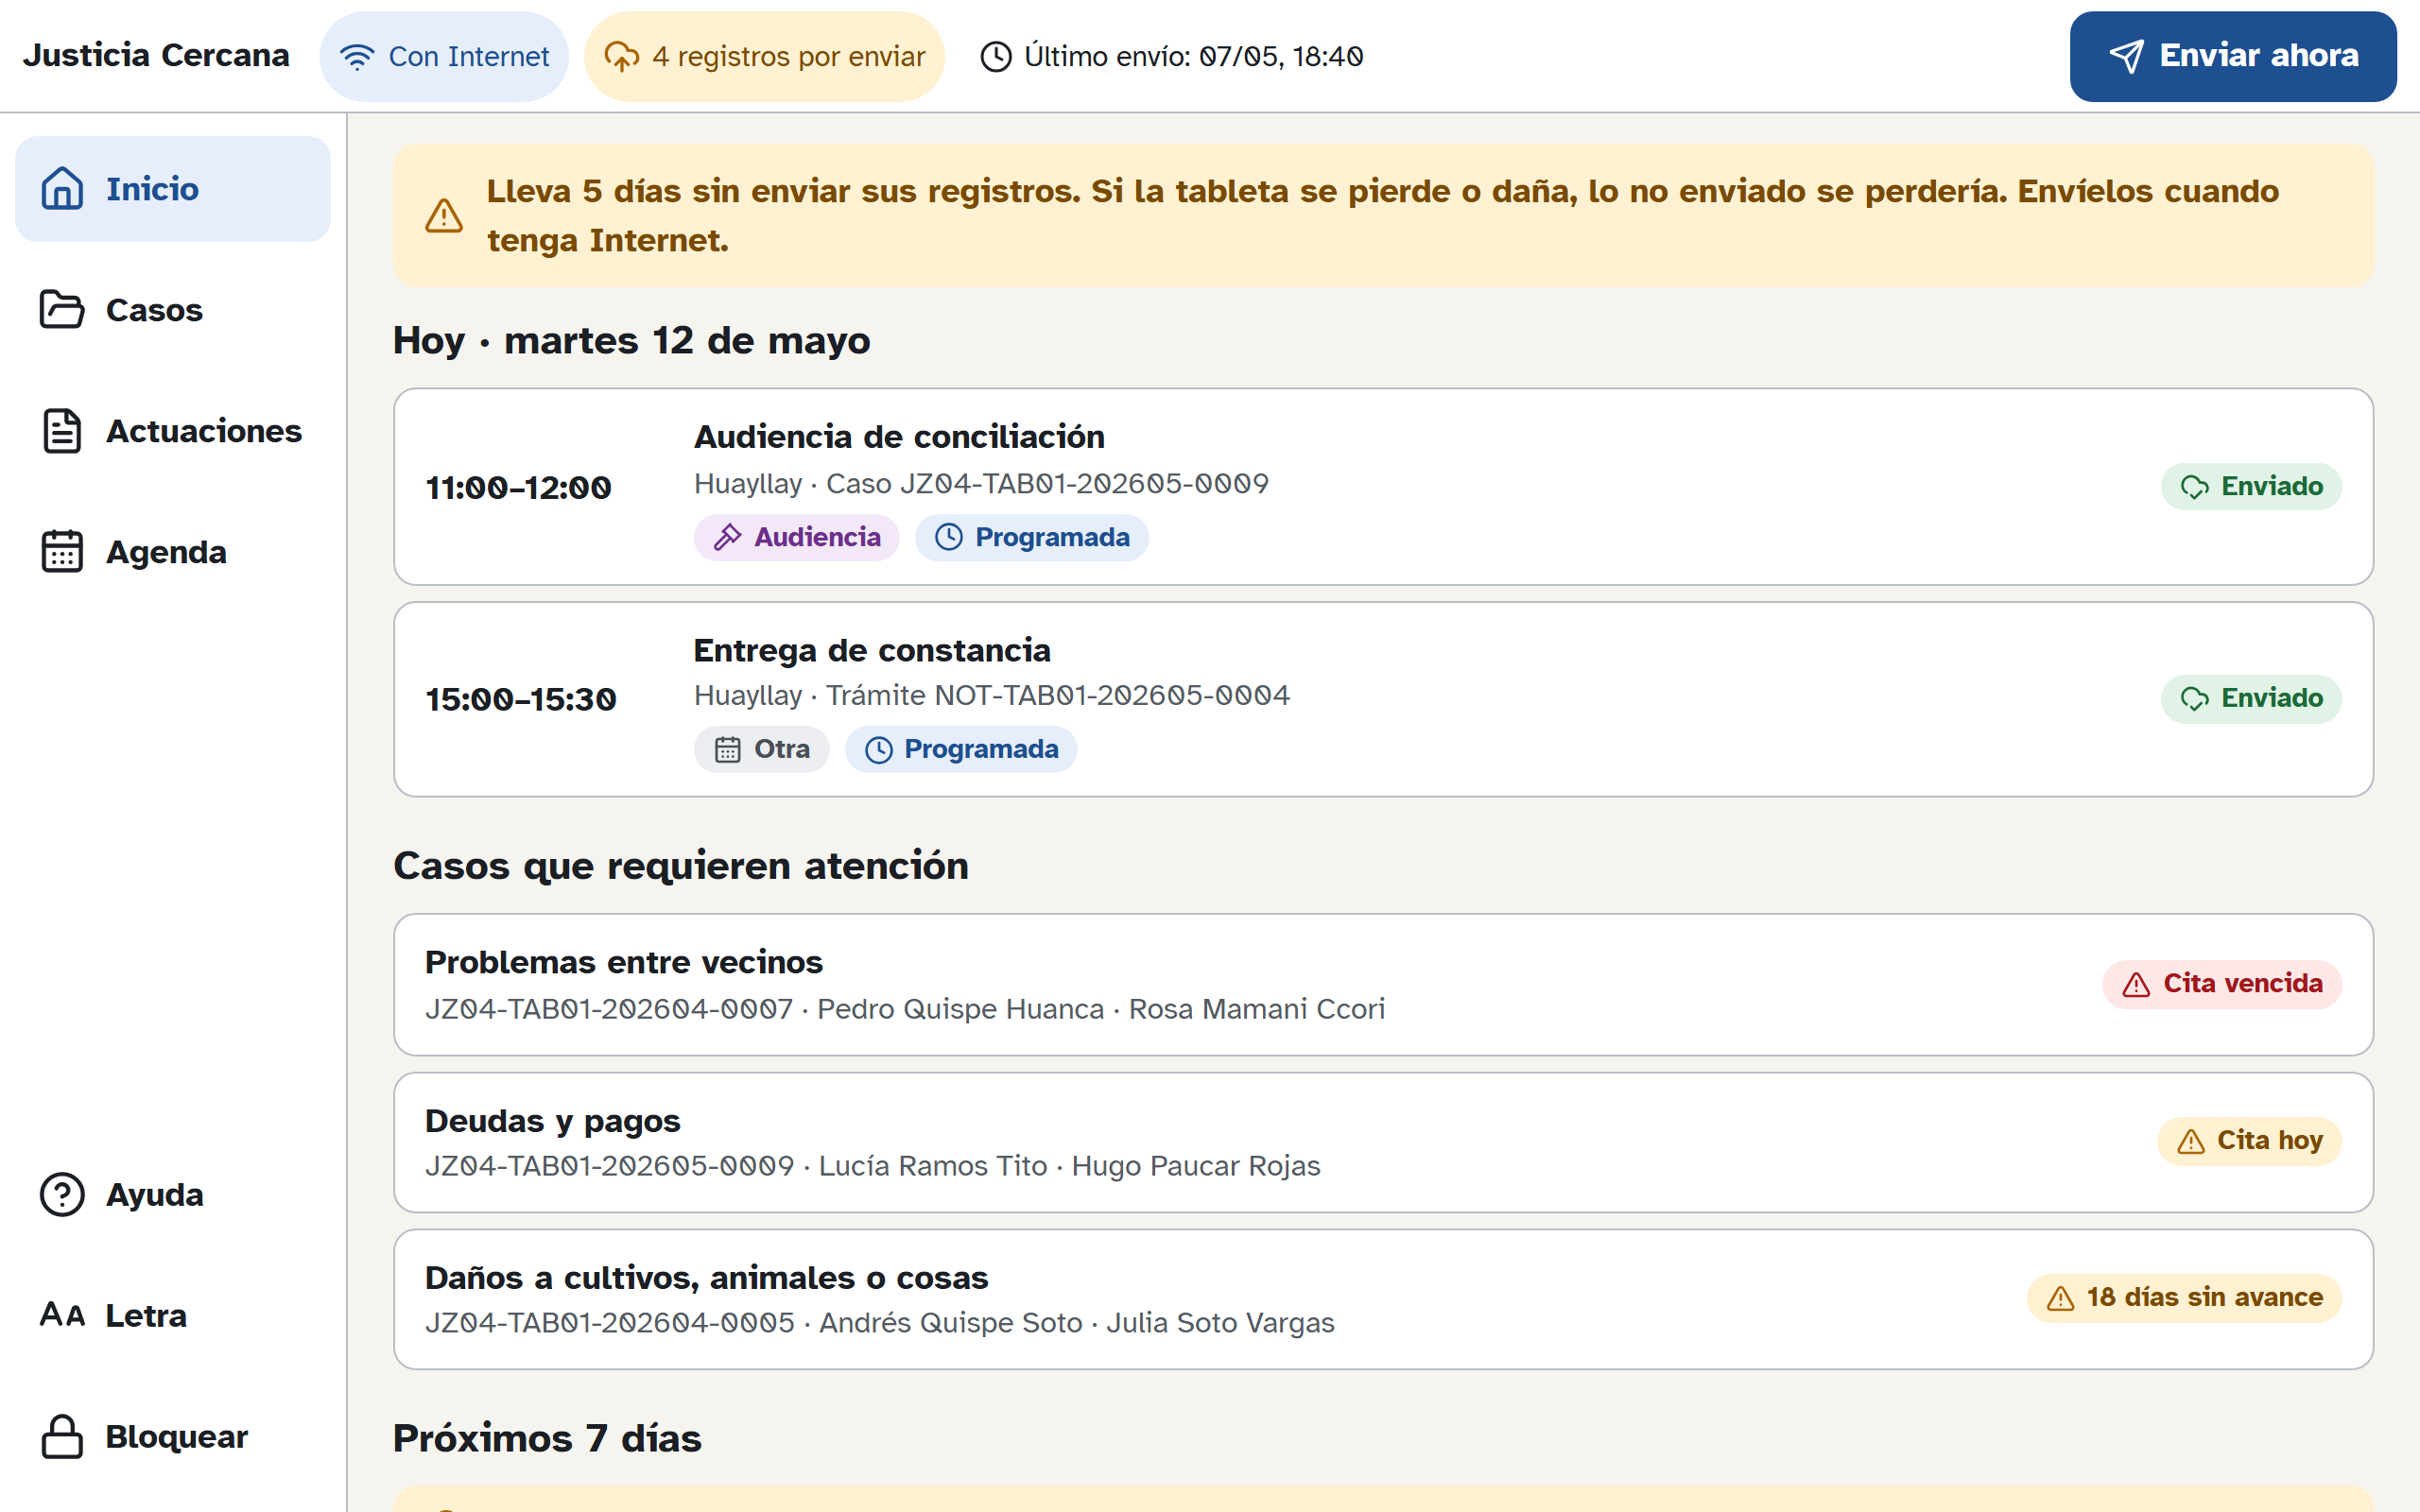
\includegraphics[width=\linewidth]{../../captures/G-05_recordatorio-dias-sin-enviar.png}\\[-2pt]{\footnotesize\raggedright\textbf{P-01.} Recordatorio ``Lleva 5 días sin enviar sus registros…'' (seed=mixed) \emph{(Funcionamiento sin conexión)}\par}\end{minipage}\par\vspace{8pt}\noindent
\begin{minipage}[t]{0.49\textwidth}\centering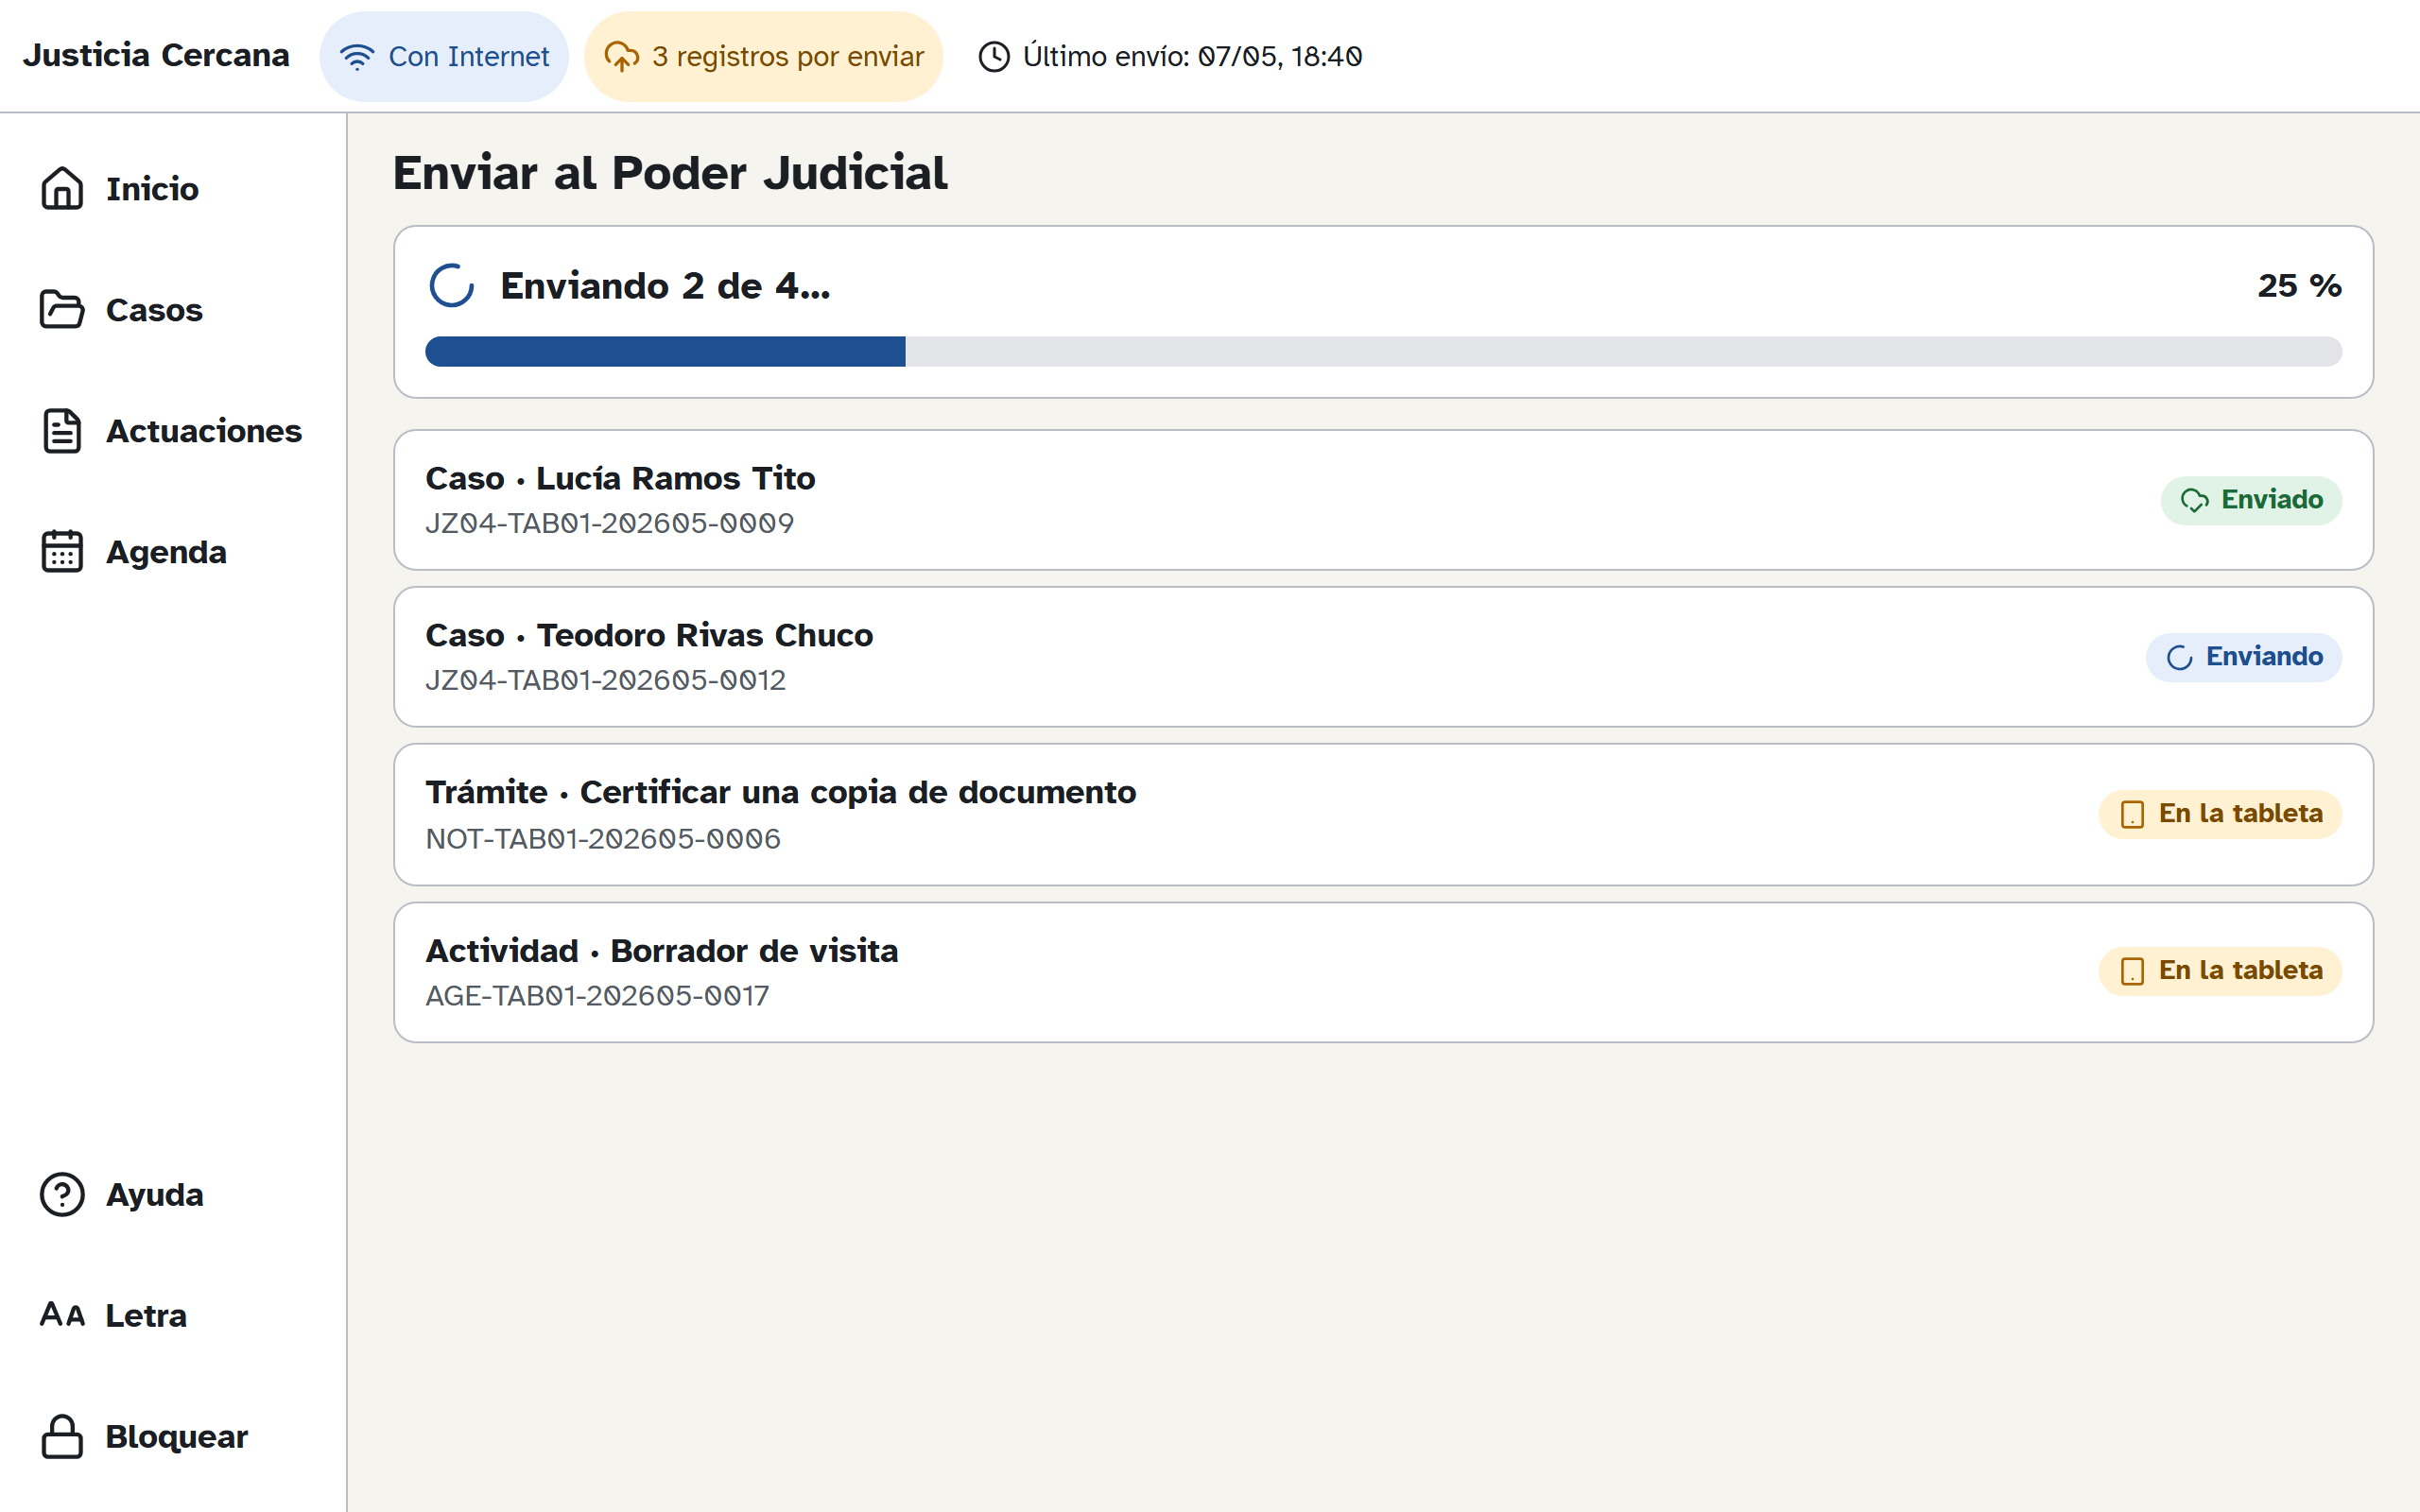
\includegraphics[width=\linewidth]{../../captures/G-06_progreso-envio.png}\\[-2pt]{\footnotesize\raggedright\textbf{P-09.} Progreso ``Enviando 2 de 4…'' con barra al 50 \% y estado por registro (freeze=1) \emph{(Funcionamiento sin conexión)}\par}\end{minipage}\hfill
\begin{minipage}[t]{0.49\textwidth}\centering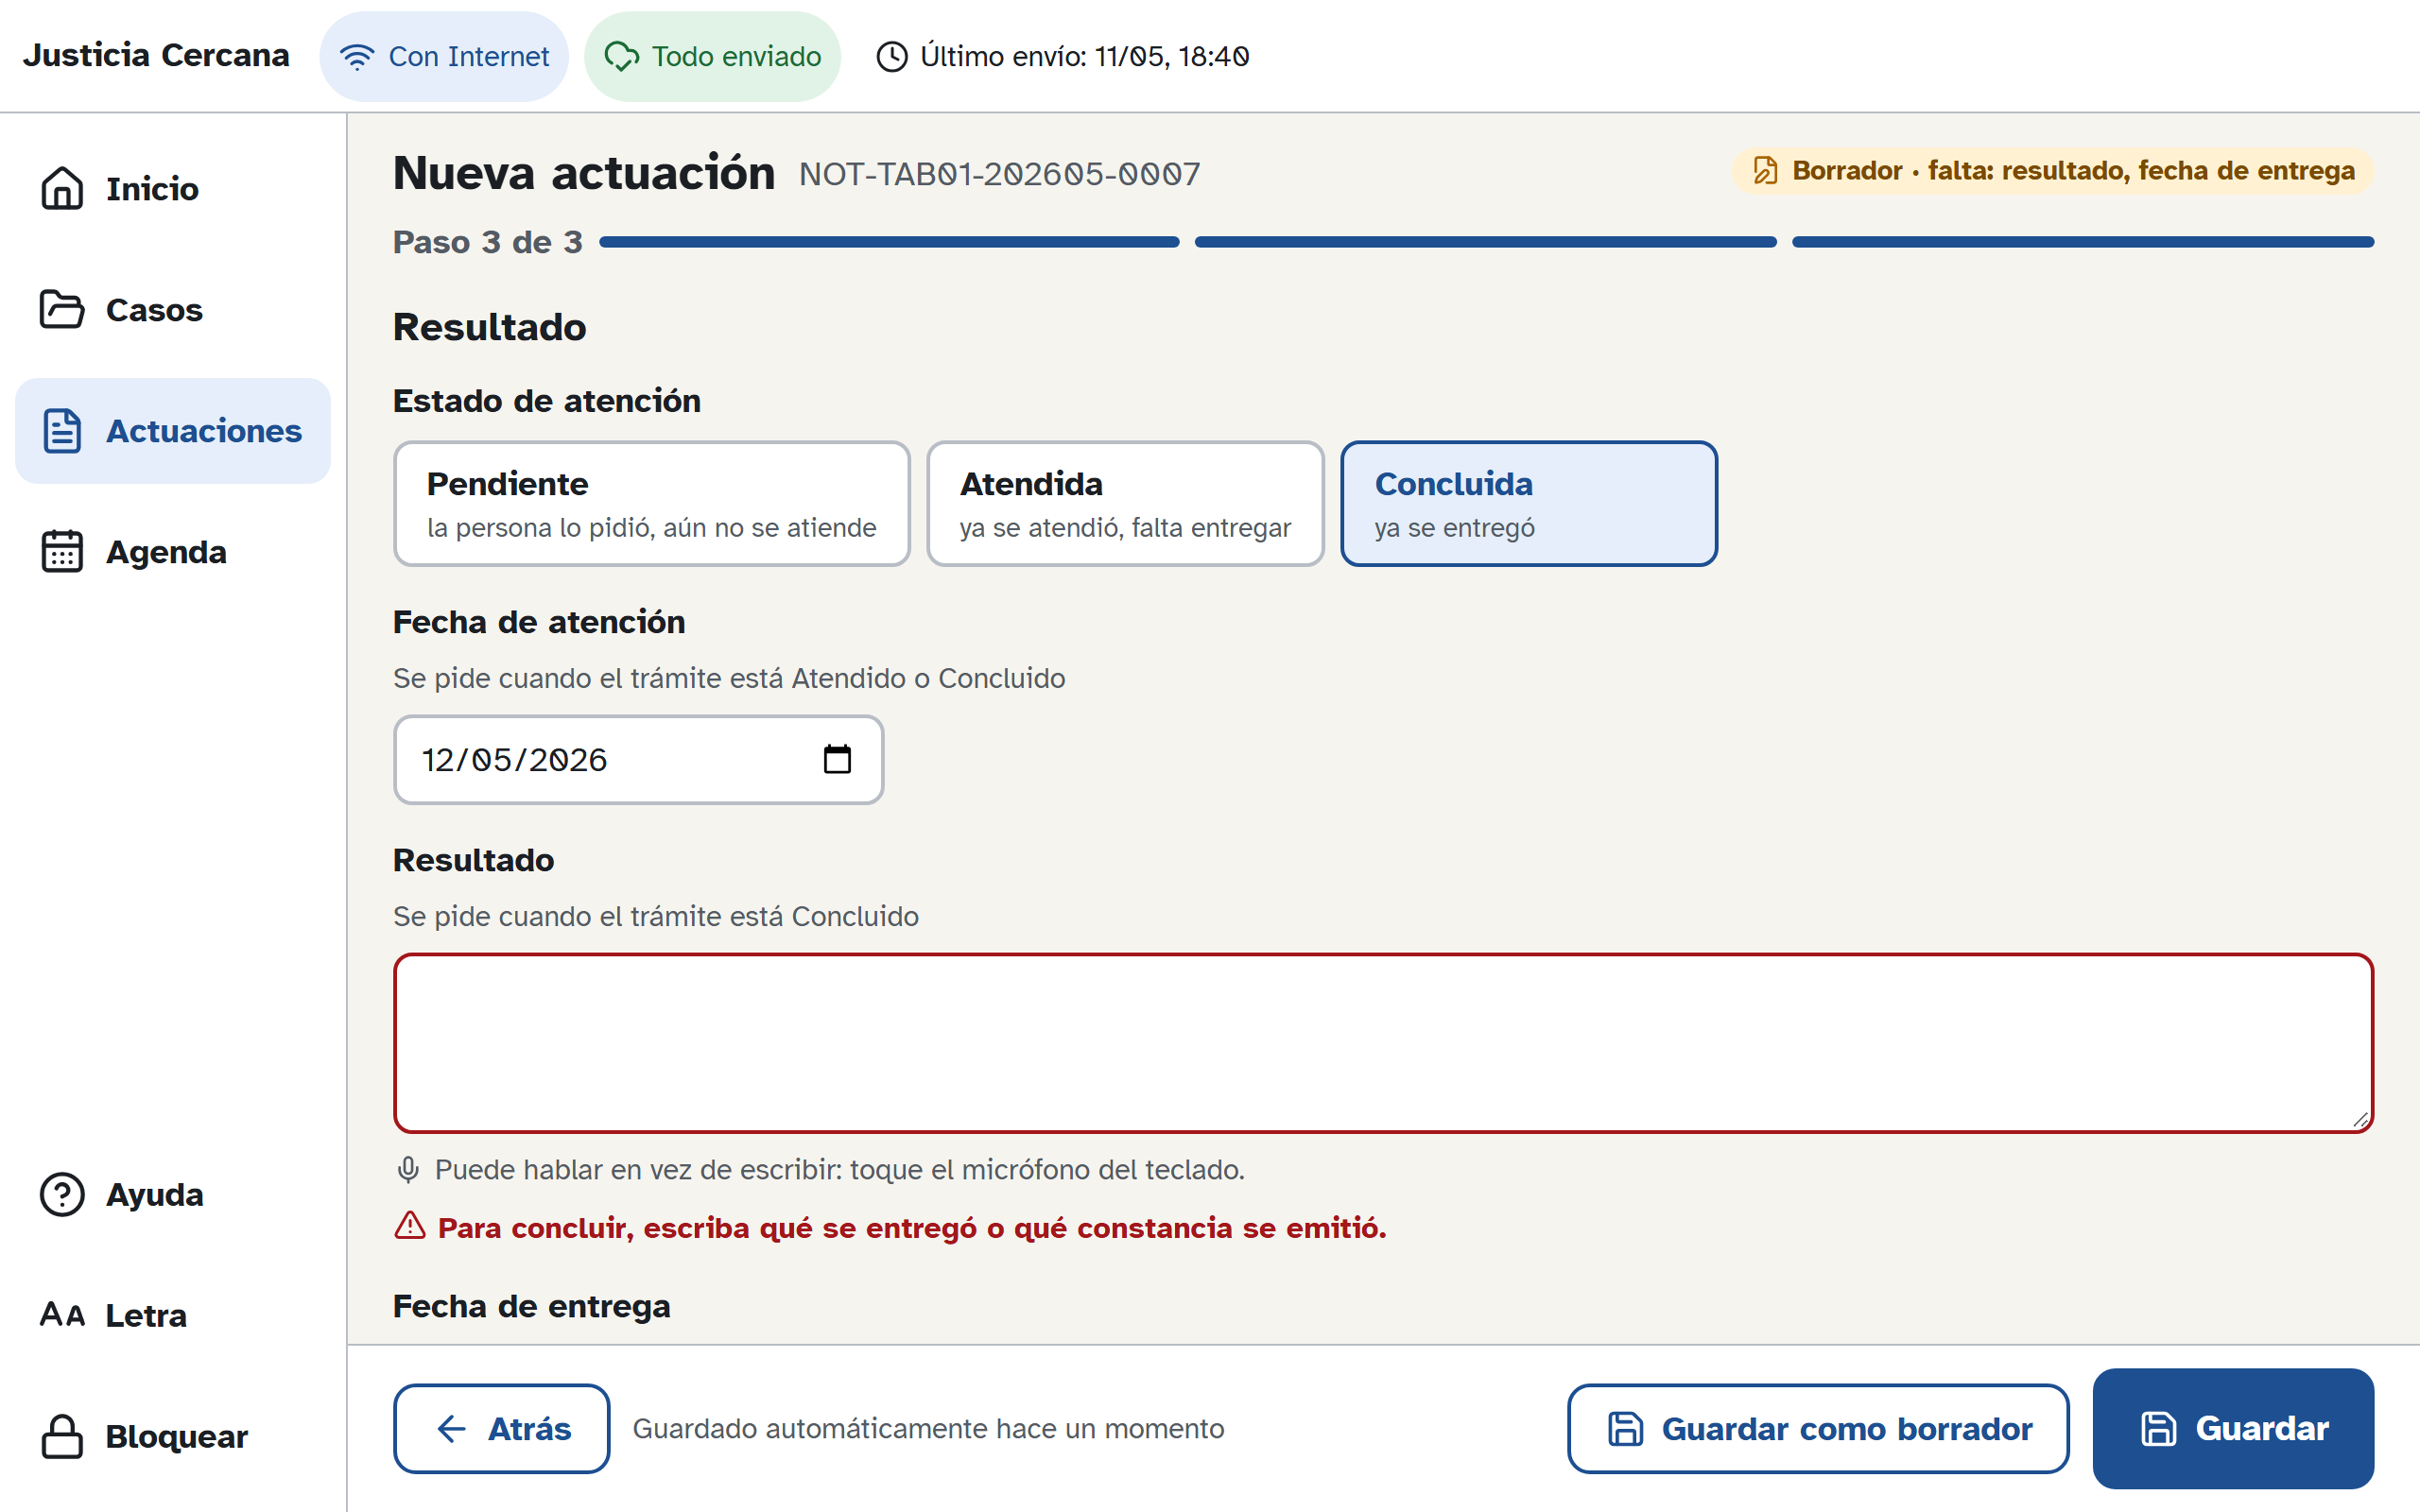
\includegraphics[width=\linewidth]{../../captures/G-07_opcional-y-condicionales.png}\\[-2pt]{\footnotesize\raggedright\textbf{P-06.} Etiquetas ``(opcional)'' y líneas de campos condicionales (``Se pide cuando…'') \emph{(Principios de diseño y heurísticas)}\par}\end{minipage}\par\vspace{8pt}\noindent
\begin{minipage}[t]{0.49\textwidth}\centering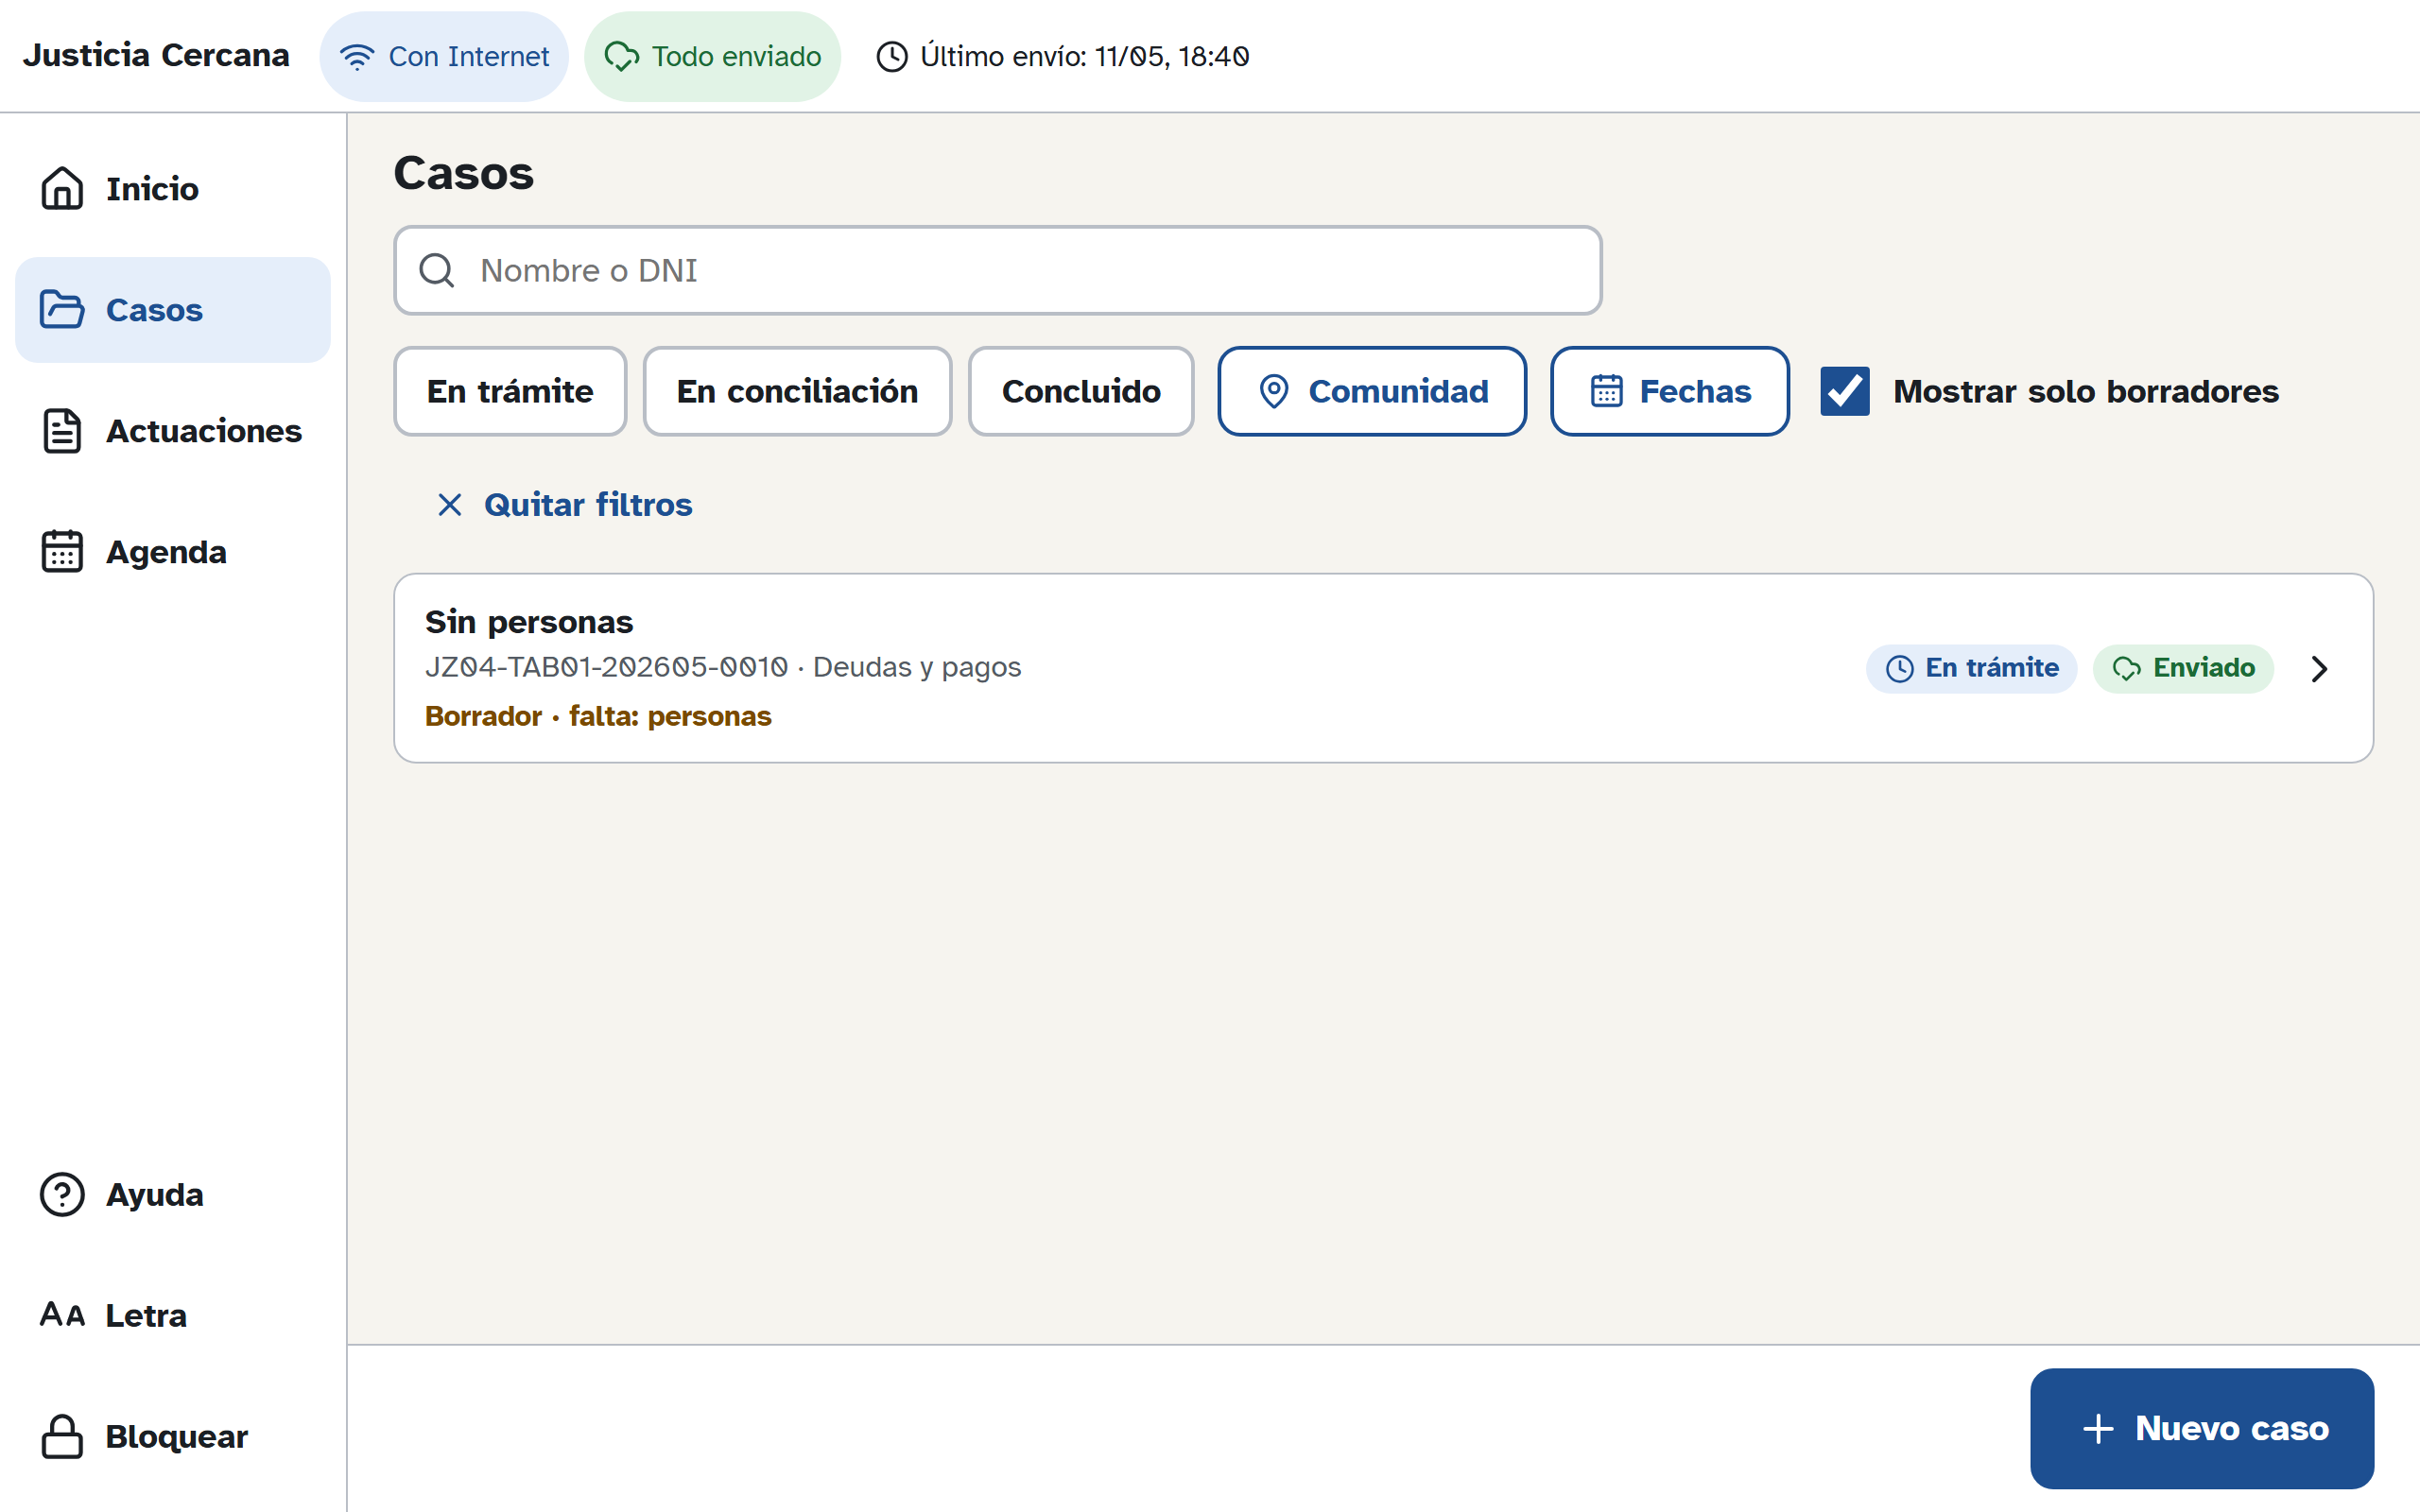
\includegraphics[width=\linewidth]{../../captures/G-08_borrador-casos.png}\\[-2pt]{\footnotesize\raggedright\textbf{P-02.} ``Borrador · falta: personas'' y casilla ``Mostrar solo borradores'' (casos) \emph{(Principios de diseño y heurísticas)}\par}\end{minipage}\hfill
\begin{minipage}[t]{0.49\textwidth}\centering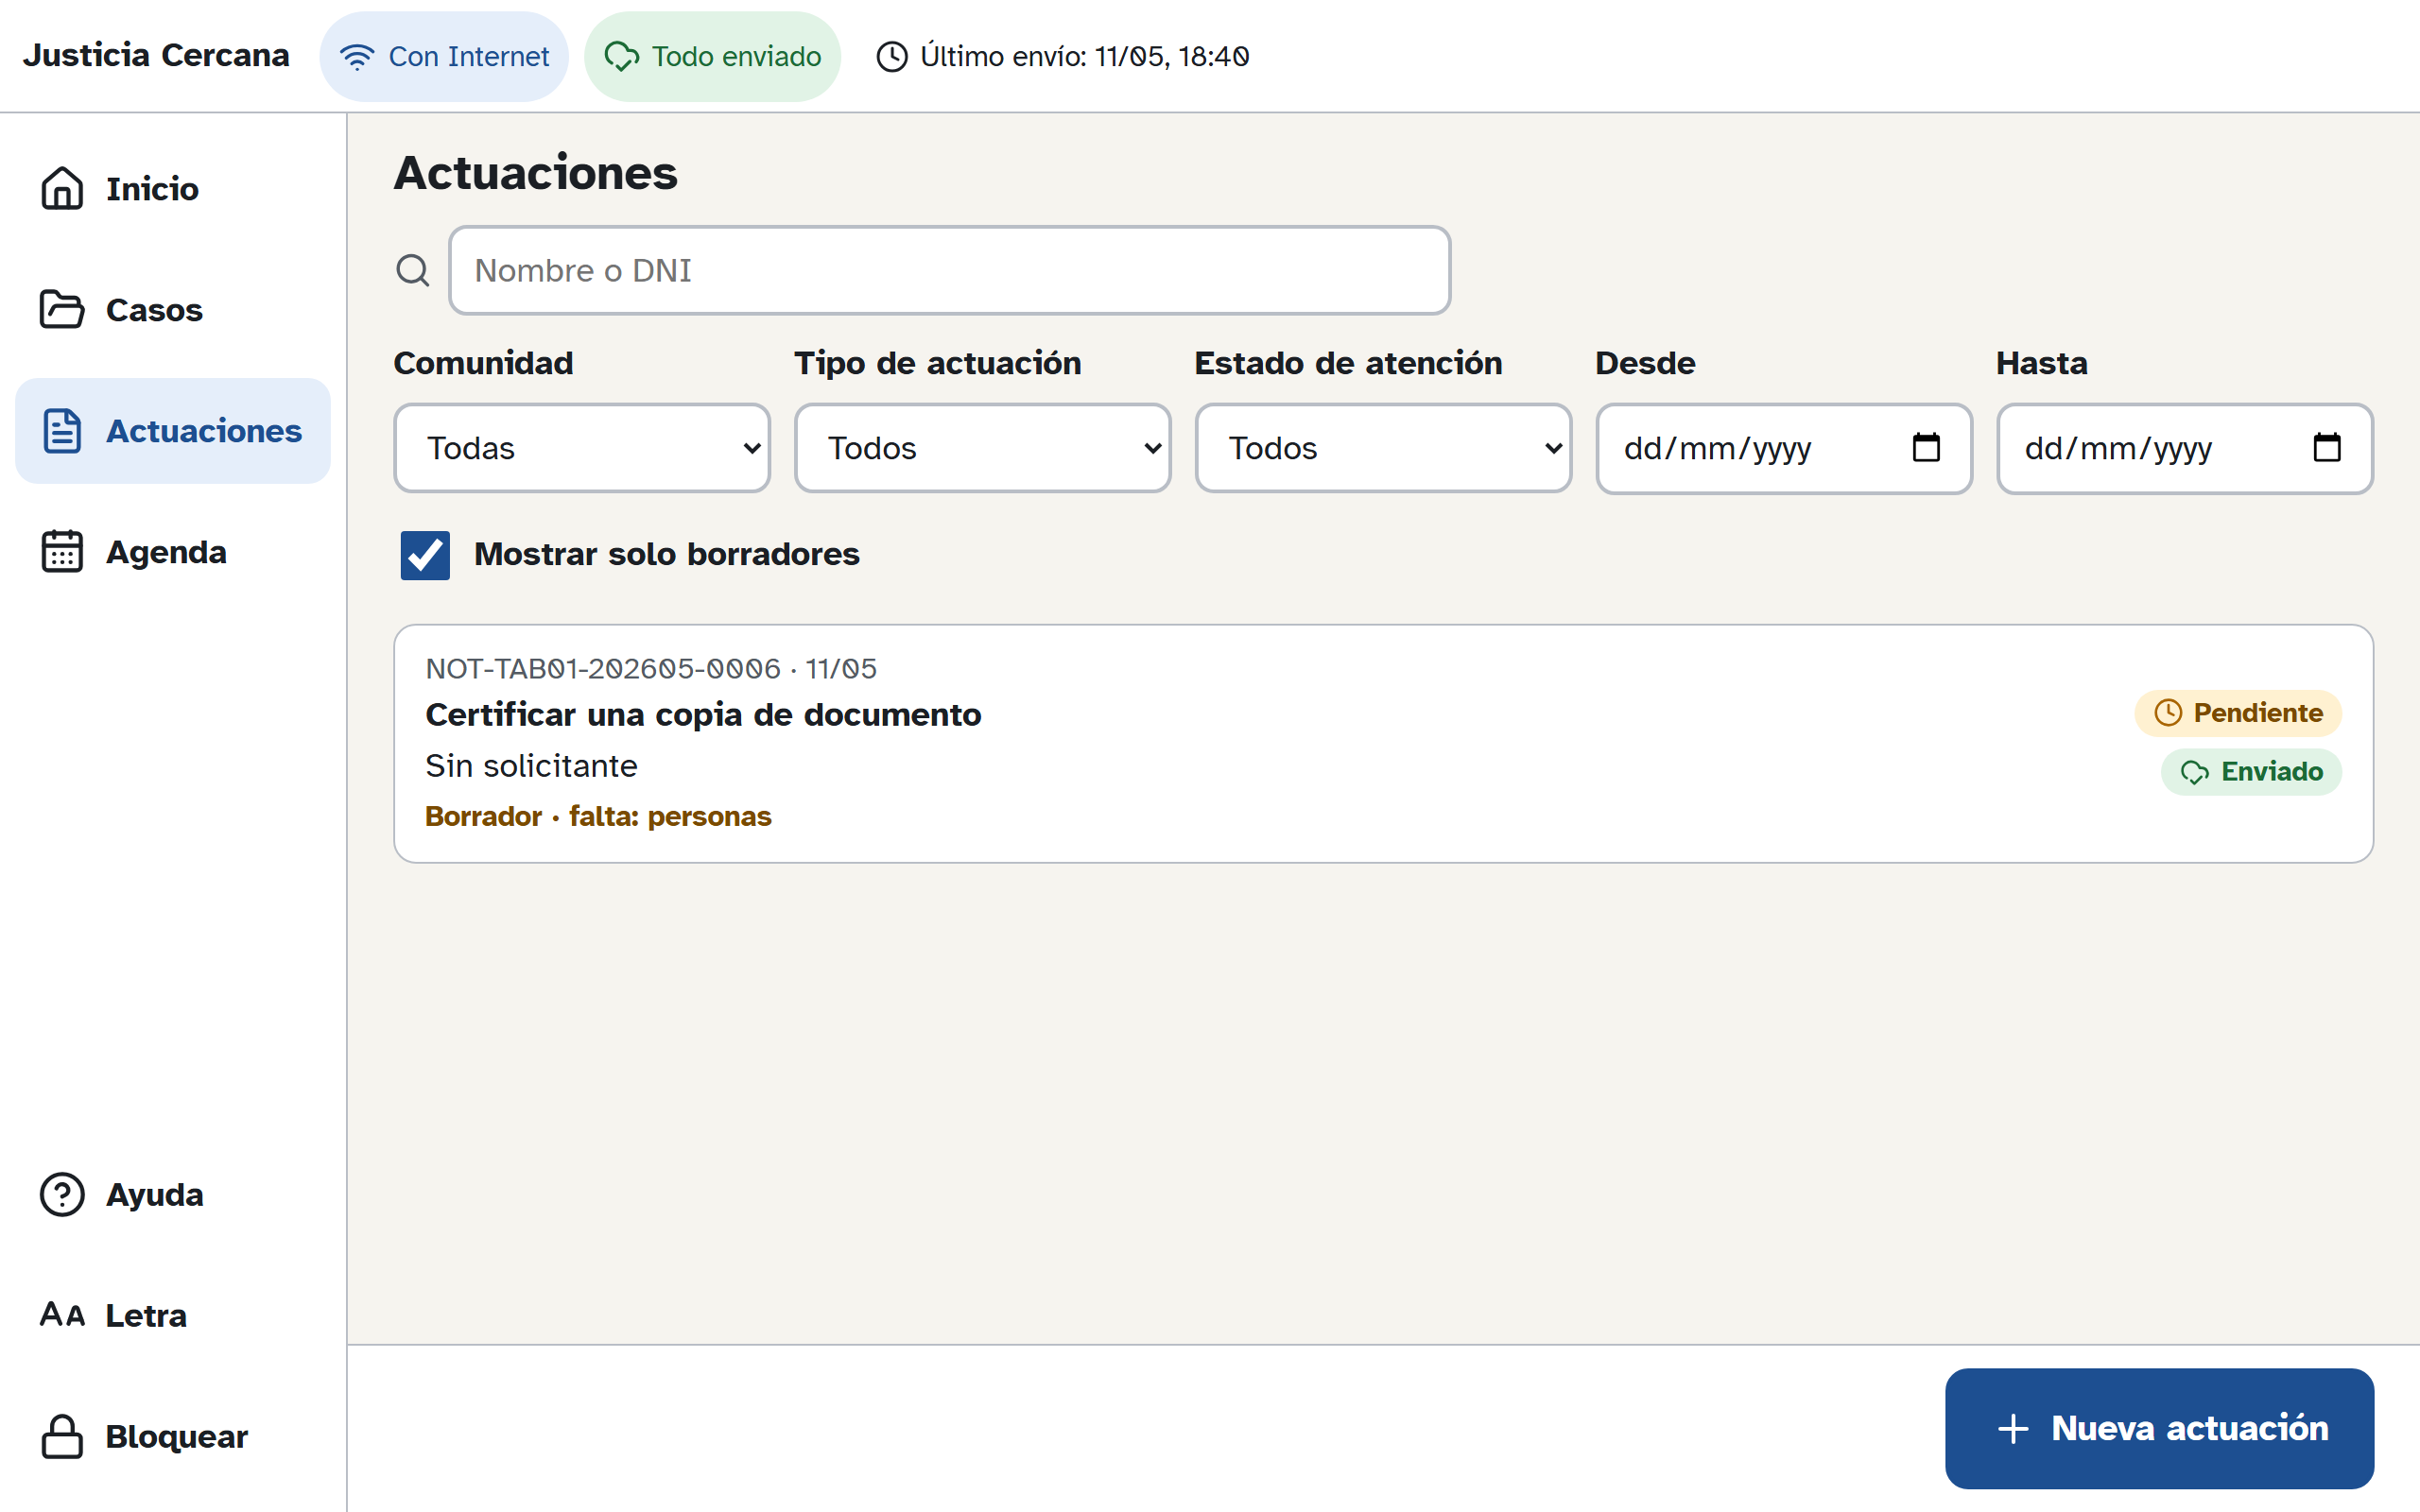
\includegraphics[width=\linewidth]{../../captures/G-09_borrador-actuaciones.png}\\[-2pt]{\footnotesize\raggedright\textbf{P-05.} ``Borrador · falta: personas'' y filtro de borradores (actuaciones) \emph{(Principios de diseño y heurísticas)}\par}\end{minipage}\par\vspace{8pt}\noindent
\begin{minipage}[t]{0.49\textwidth}\centering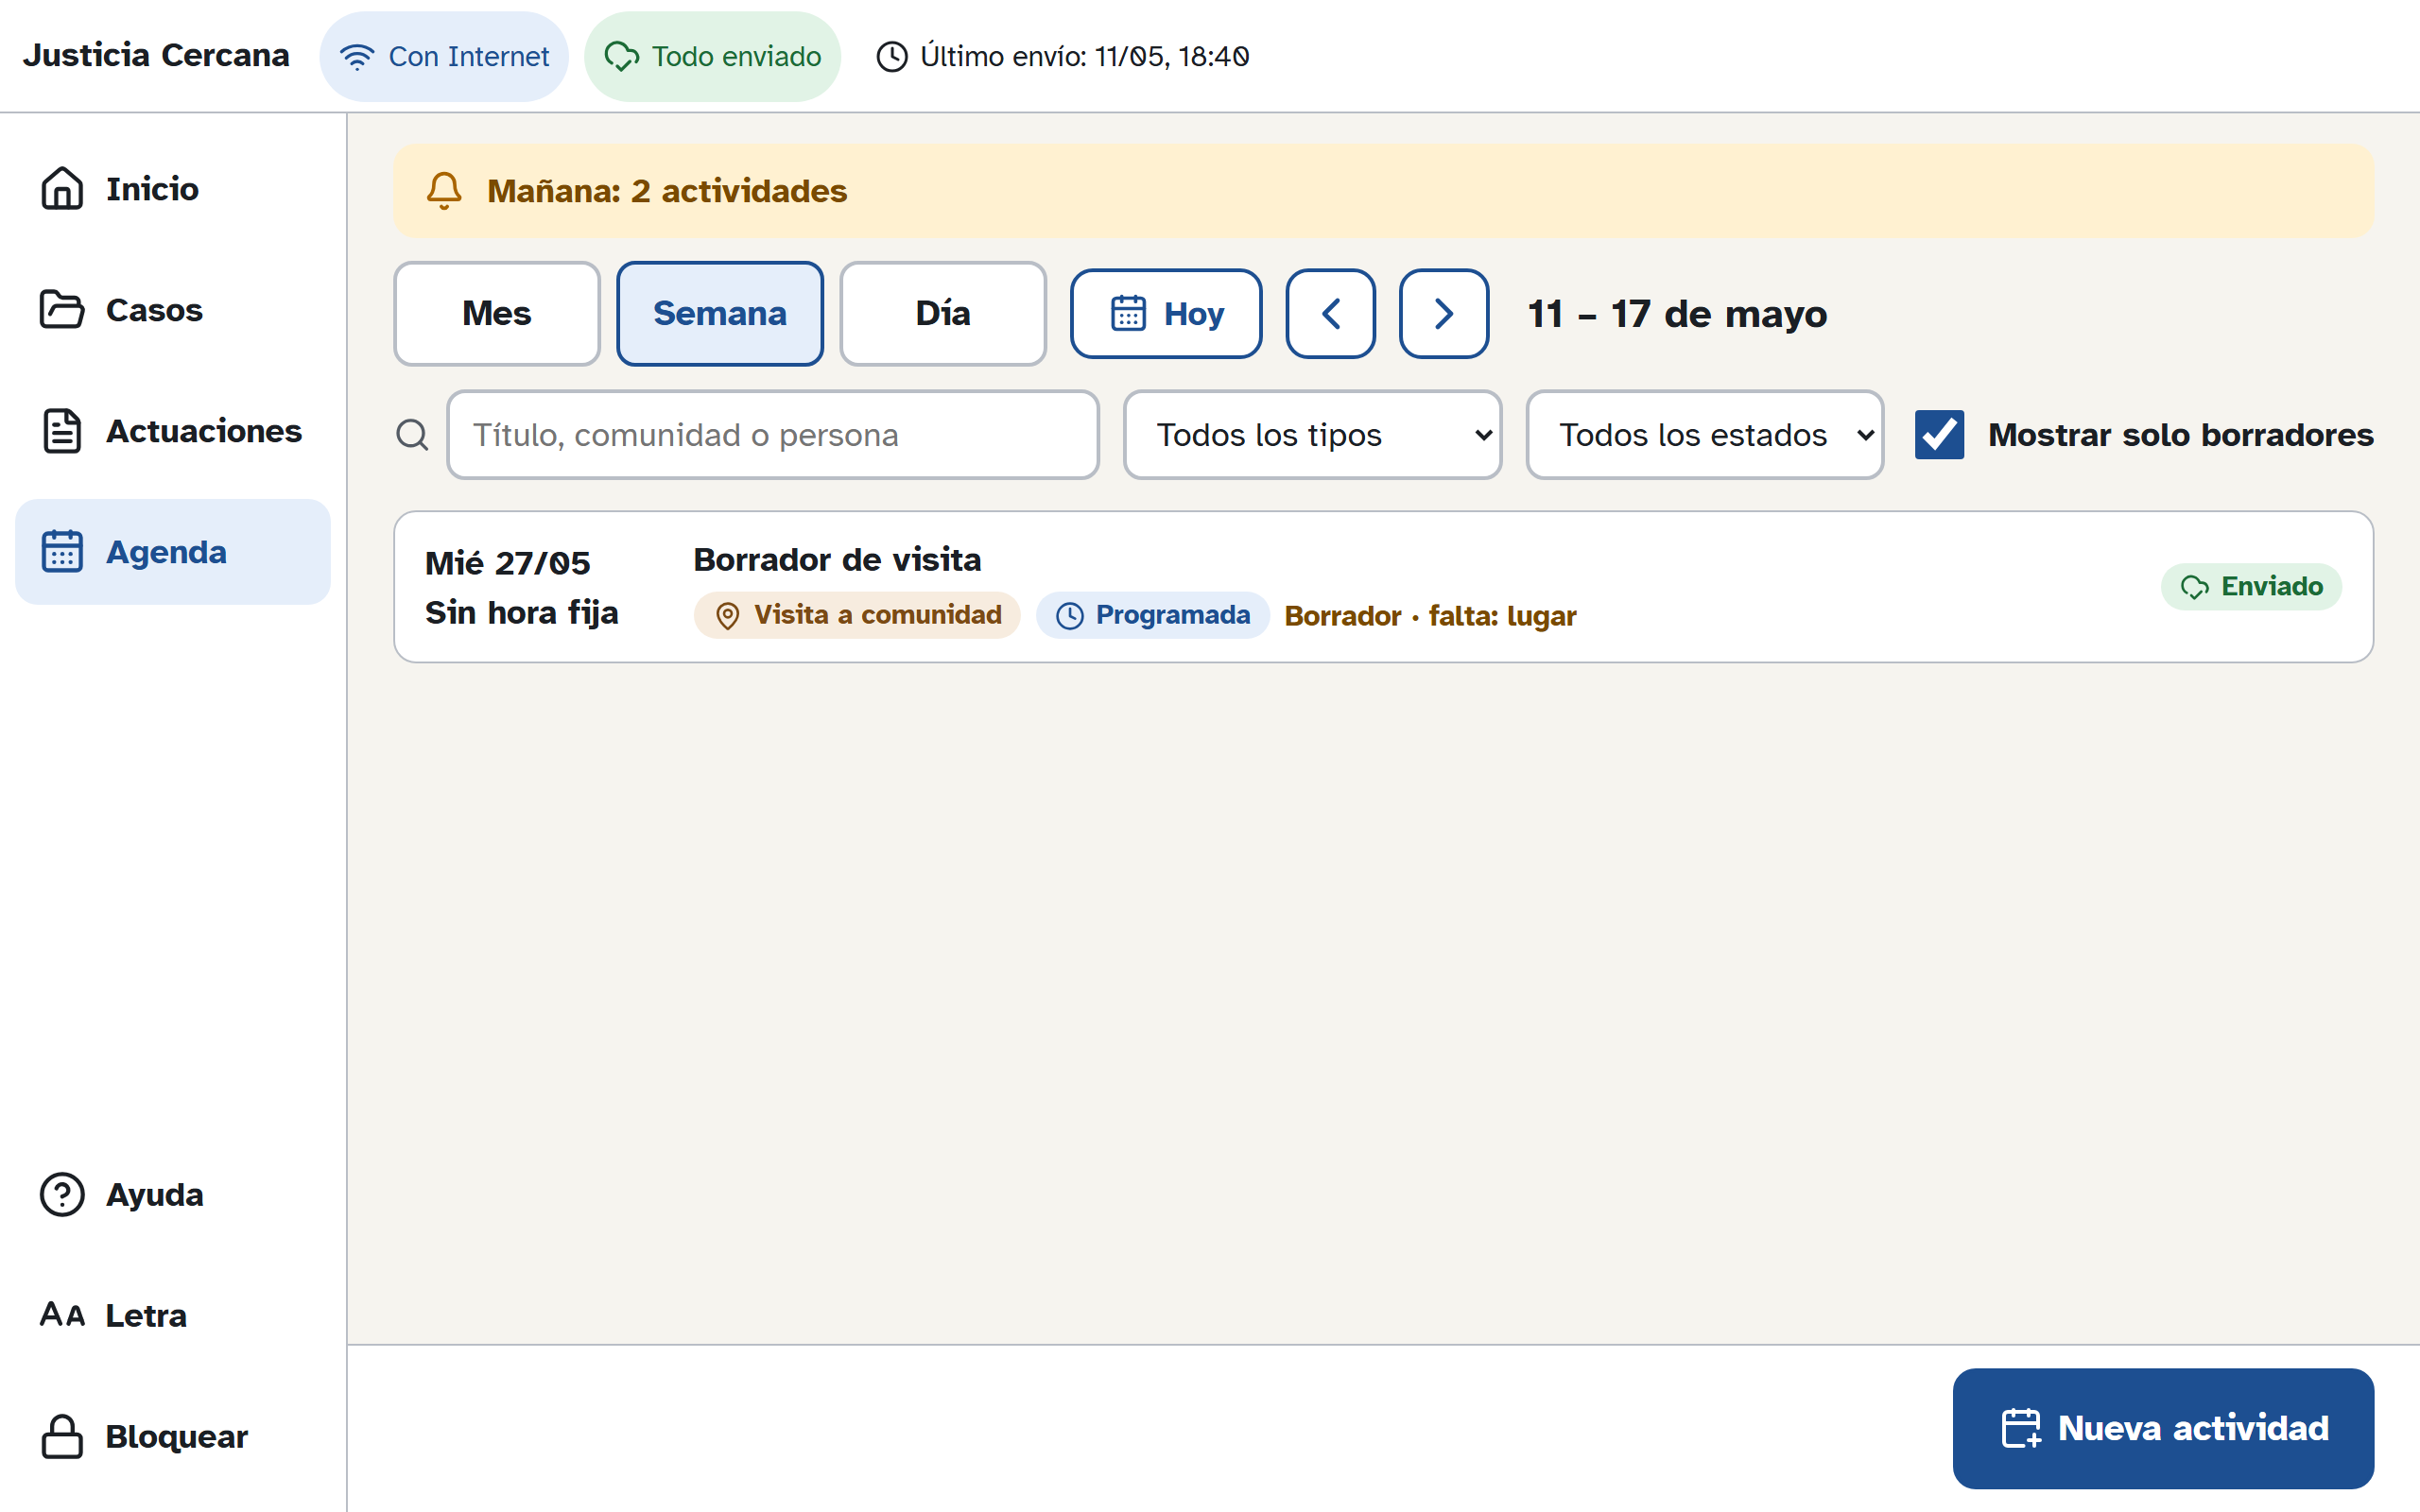
\includegraphics[width=\linewidth]{../../captures/G-10_borrador-agenda.png}\\[-2pt]{\footnotesize\raggedright\textbf{P-07.} ``Borrador · falta: lugar'' y filtro de borradores (agenda) \emph{(Principios de diseño y heurísticas)}\par}\end{minipage}\hfill
\begin{minipage}[t]{0.49\textwidth}\centering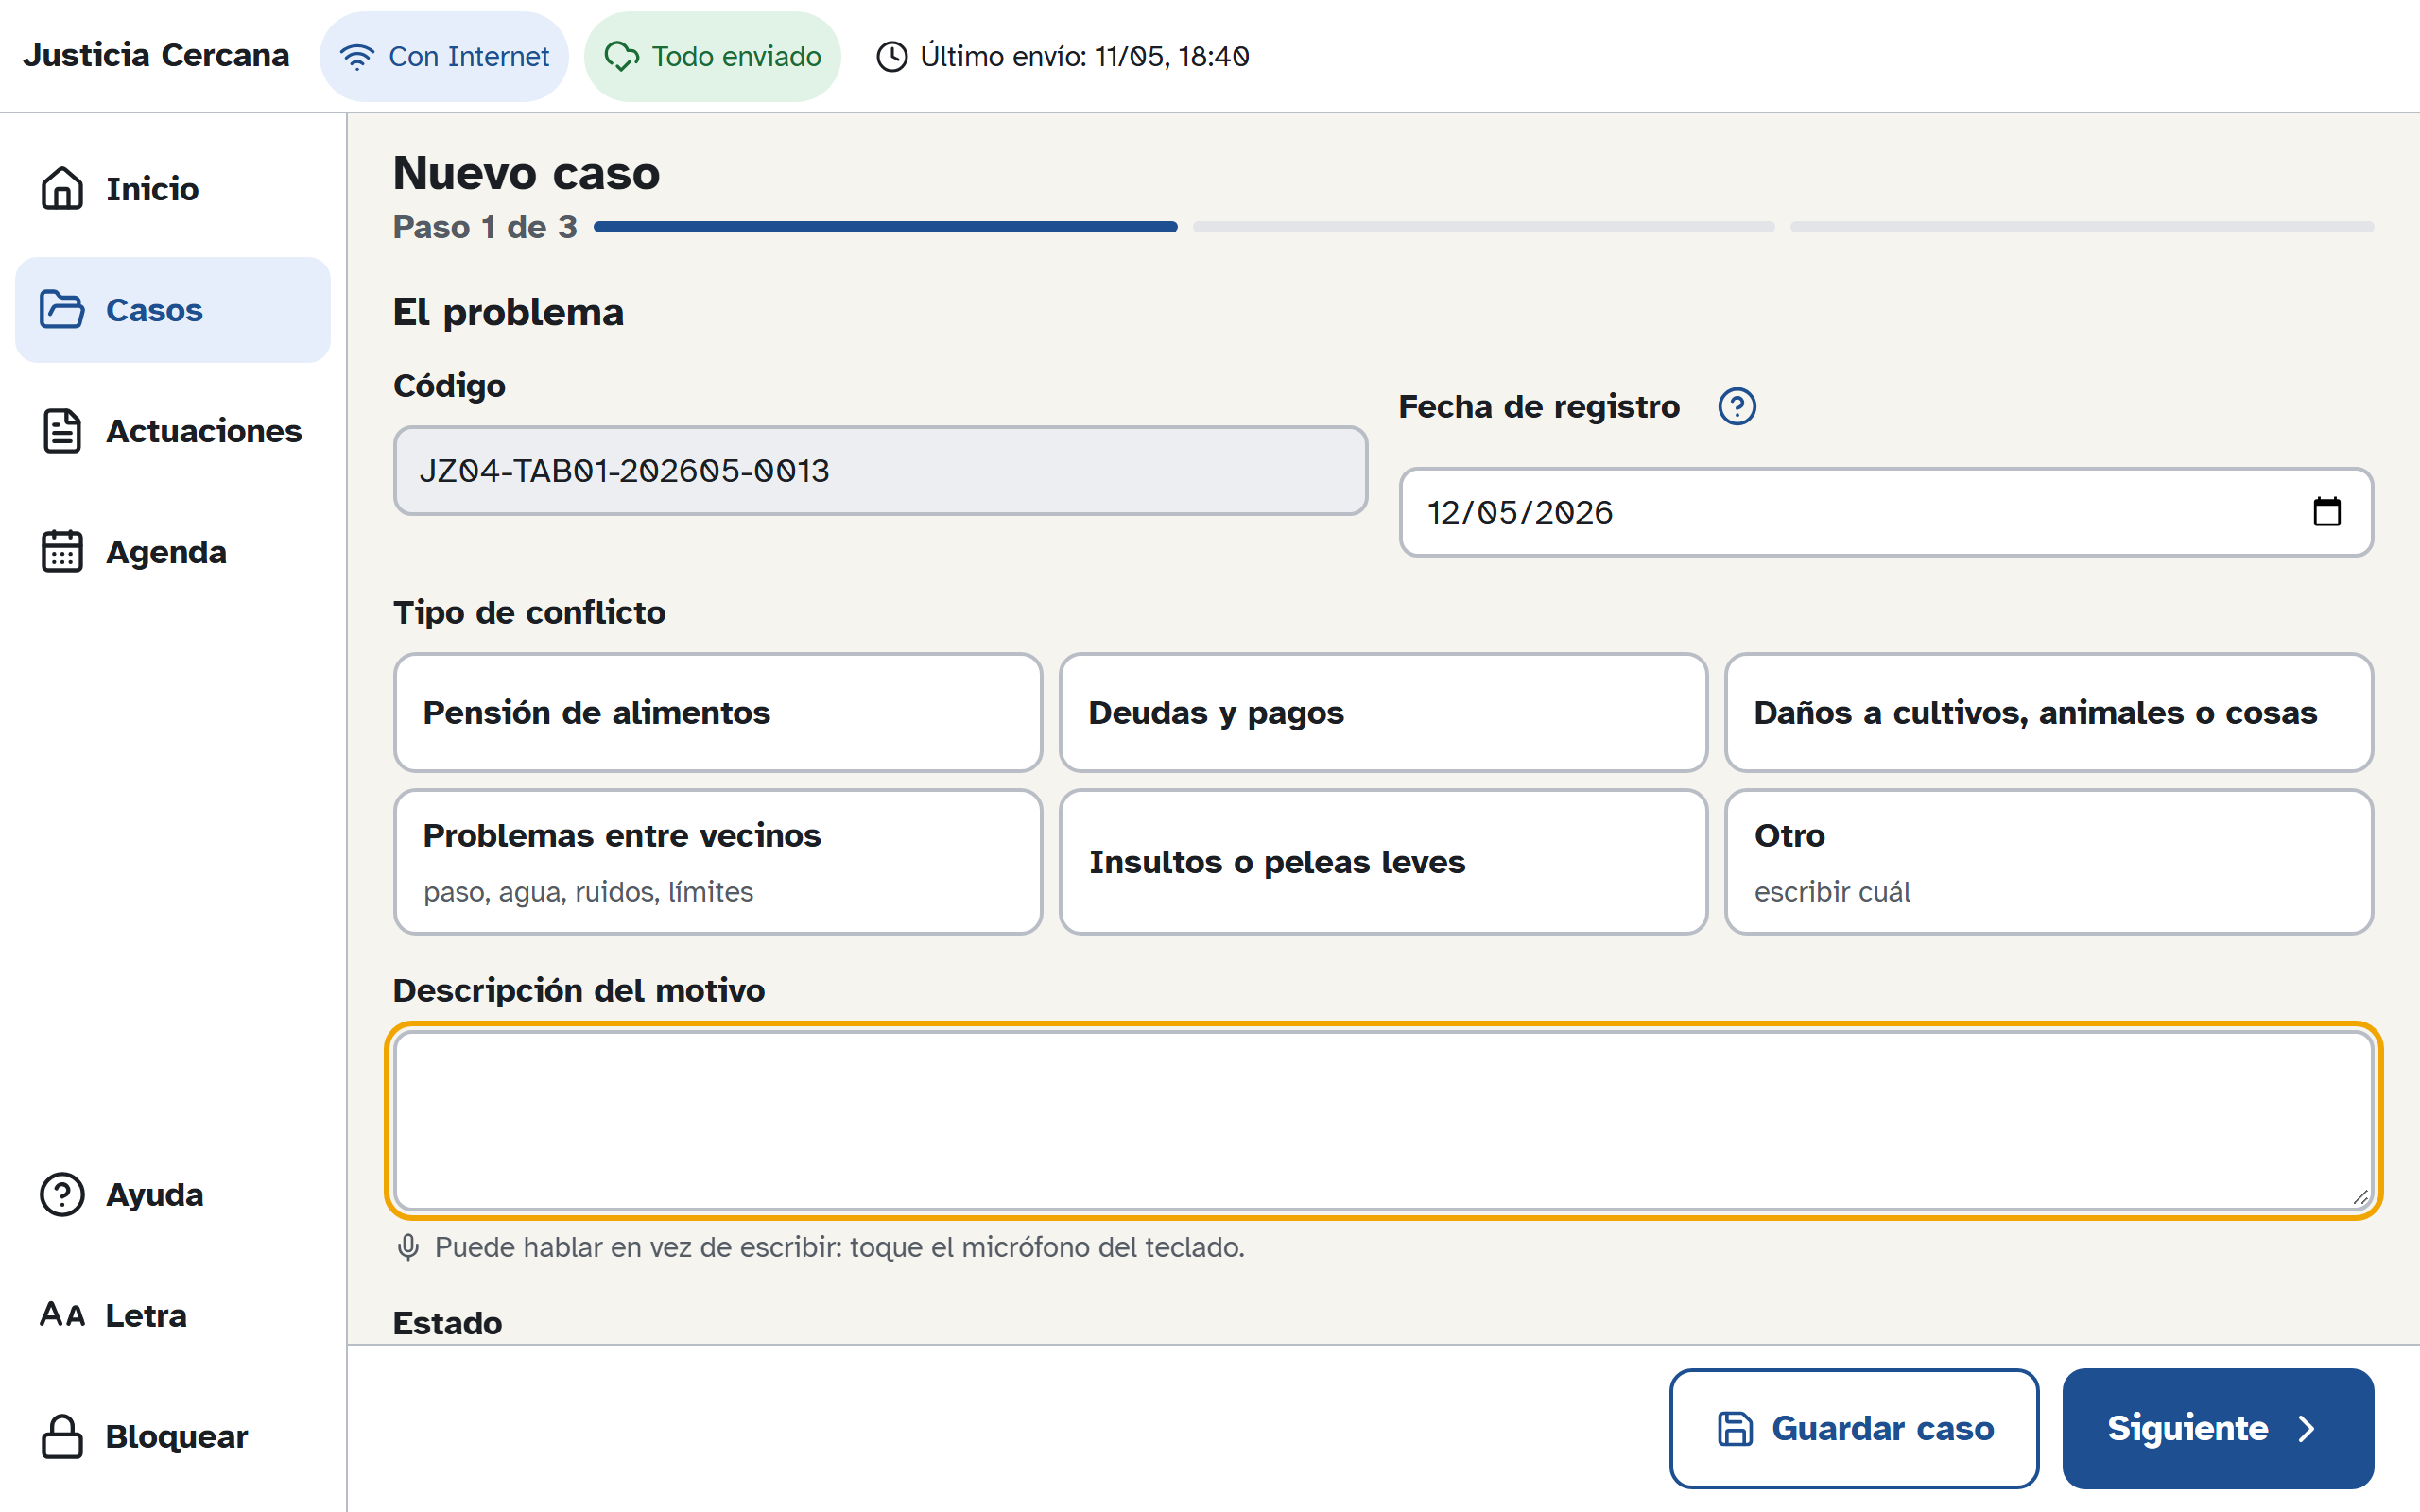
\includegraphics[width=\linewidth]{../../captures/G-11_ayuda-dictado.png}\\[-2pt]{\footnotesize\raggedright\textbf{P-03.} Ayuda de dictado del teclado bajo el campo largo (sin micrófono propio) \emph{(Factores humanos y dispositivo)}\par}\end{minipage}\par\vspace{8pt}\noindent
\begin{minipage}[t]{0.49\textwidth}\centering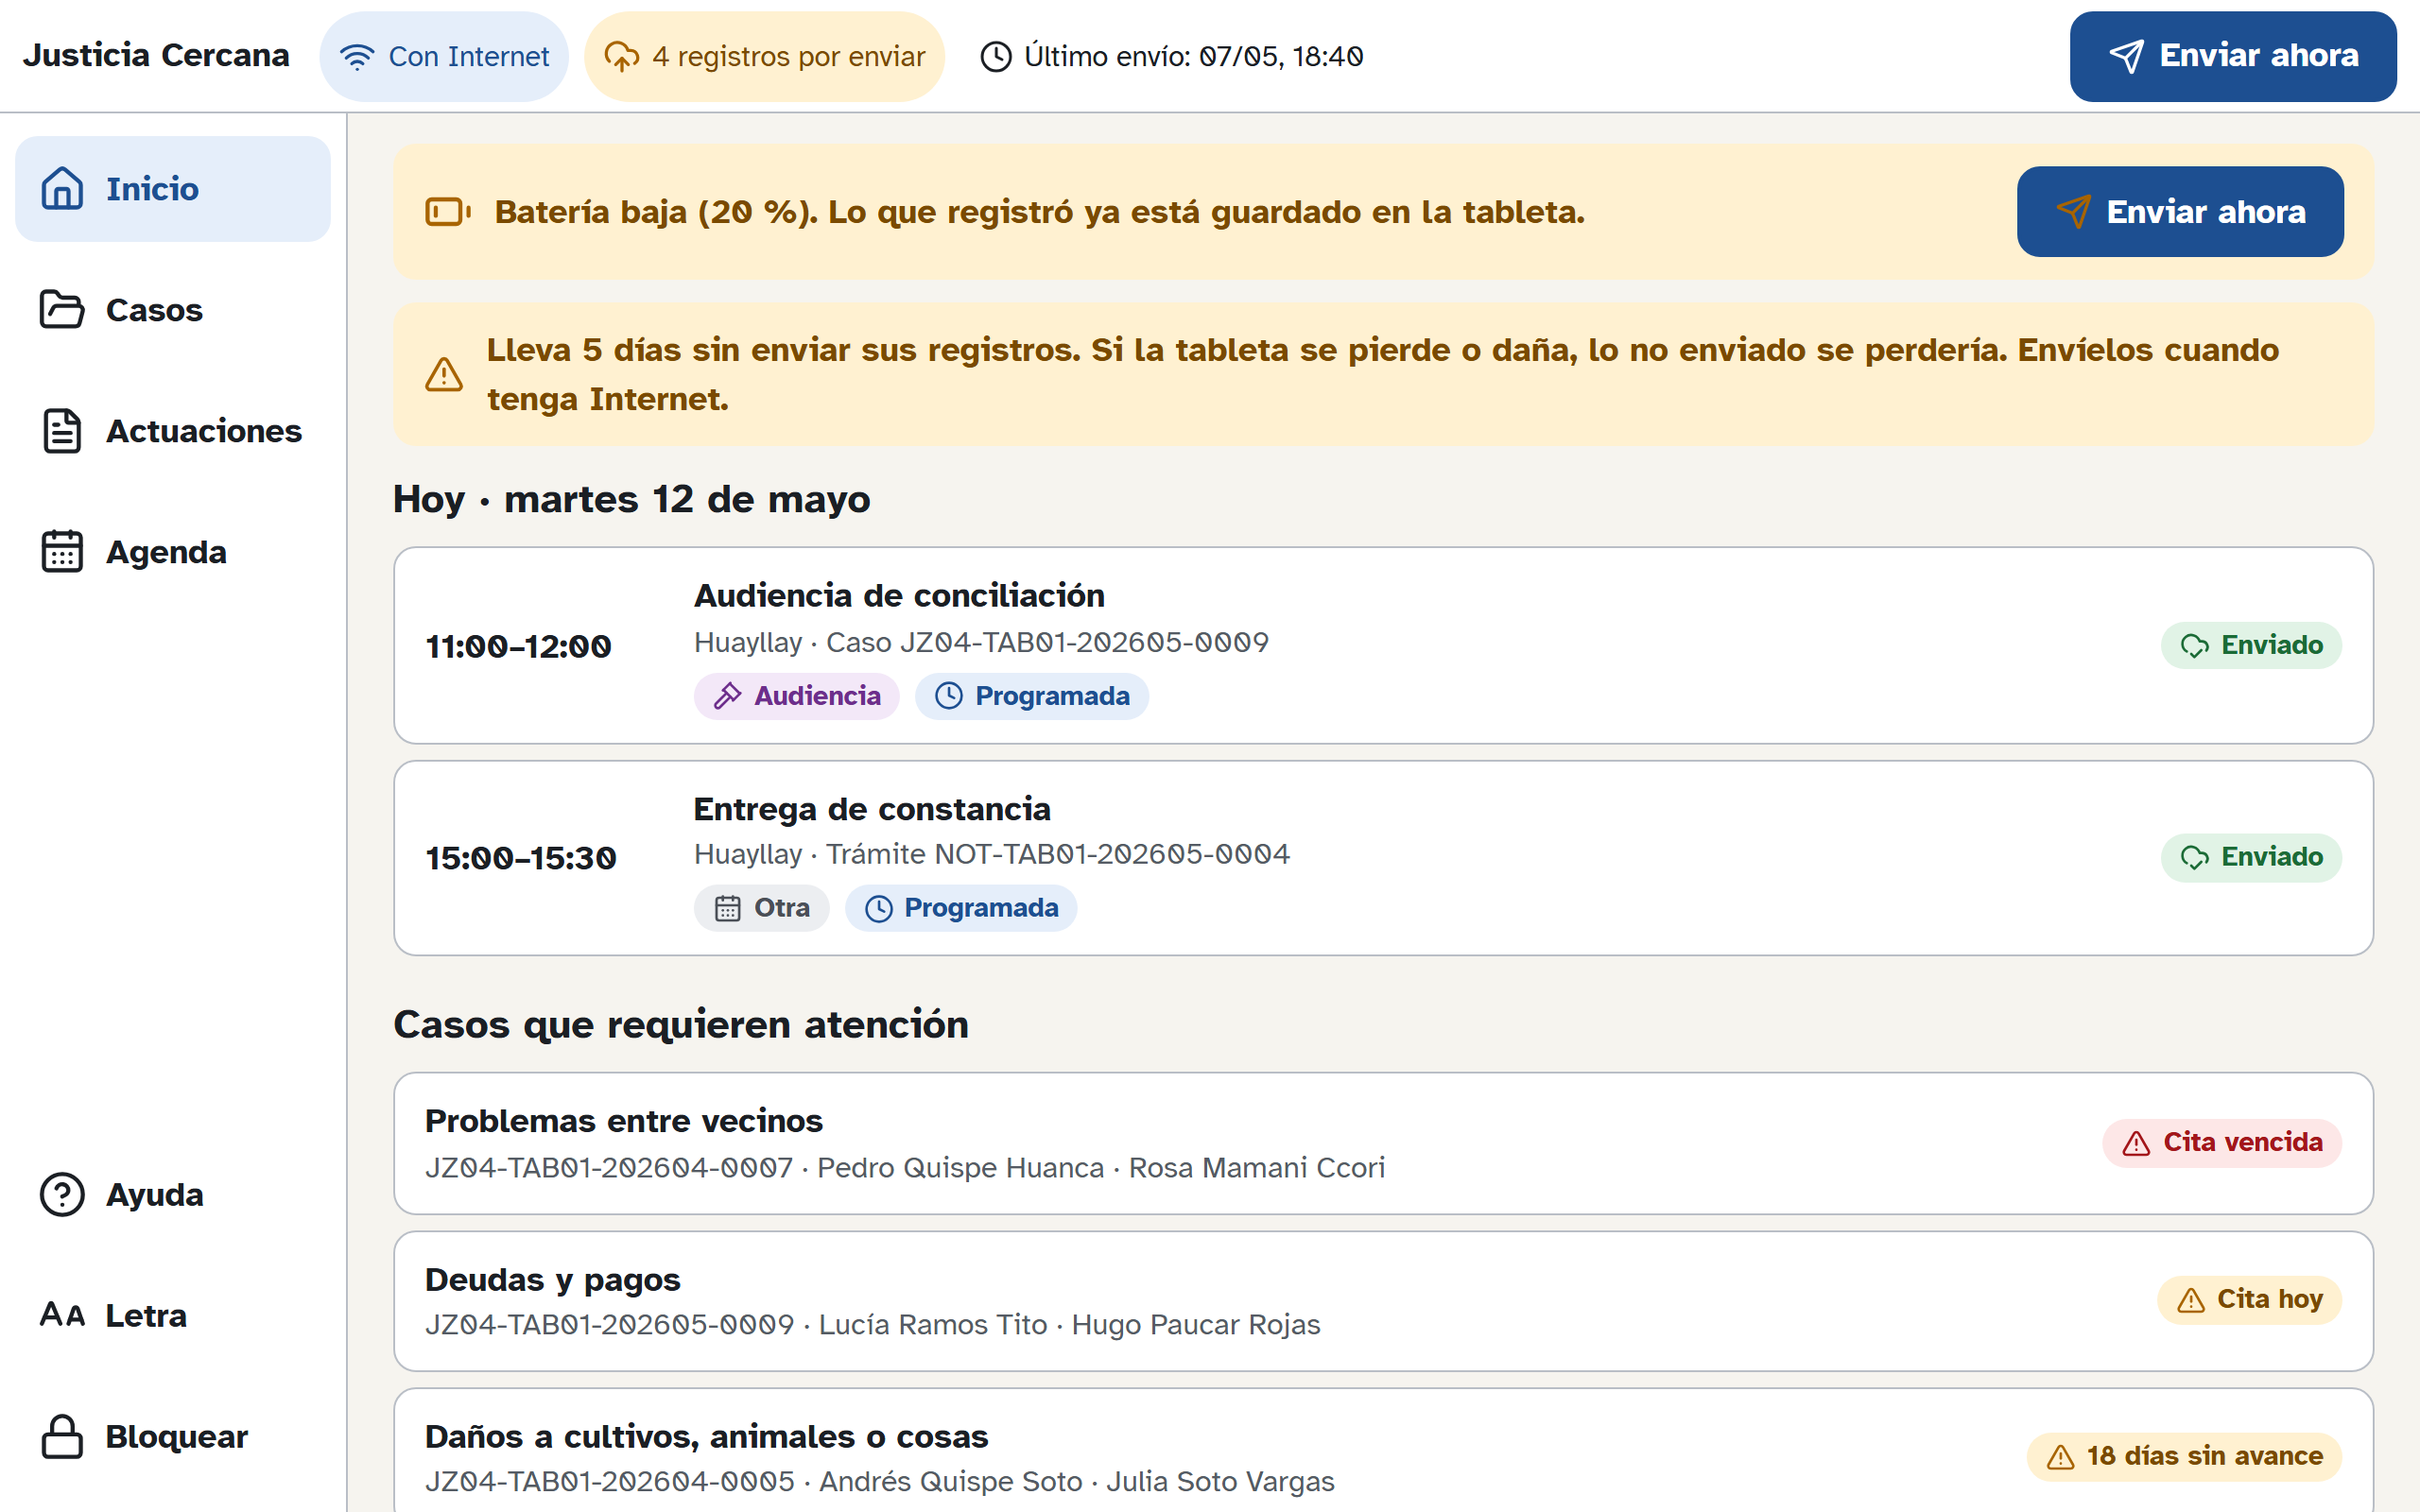
\includegraphics[width=\linewidth]{../../captures/G-12_bateria-20.png}\\[-2pt]{\footnotesize\raggedright\textbf{P-01.} Batería baja 20 \%: lo registrado ya está en la tableta; [Enviar ahora] \emph{(Factores humanos y dispositivo)}\par}\end{minipage}\hfill
\begin{minipage}[t]{0.49\textwidth}\centering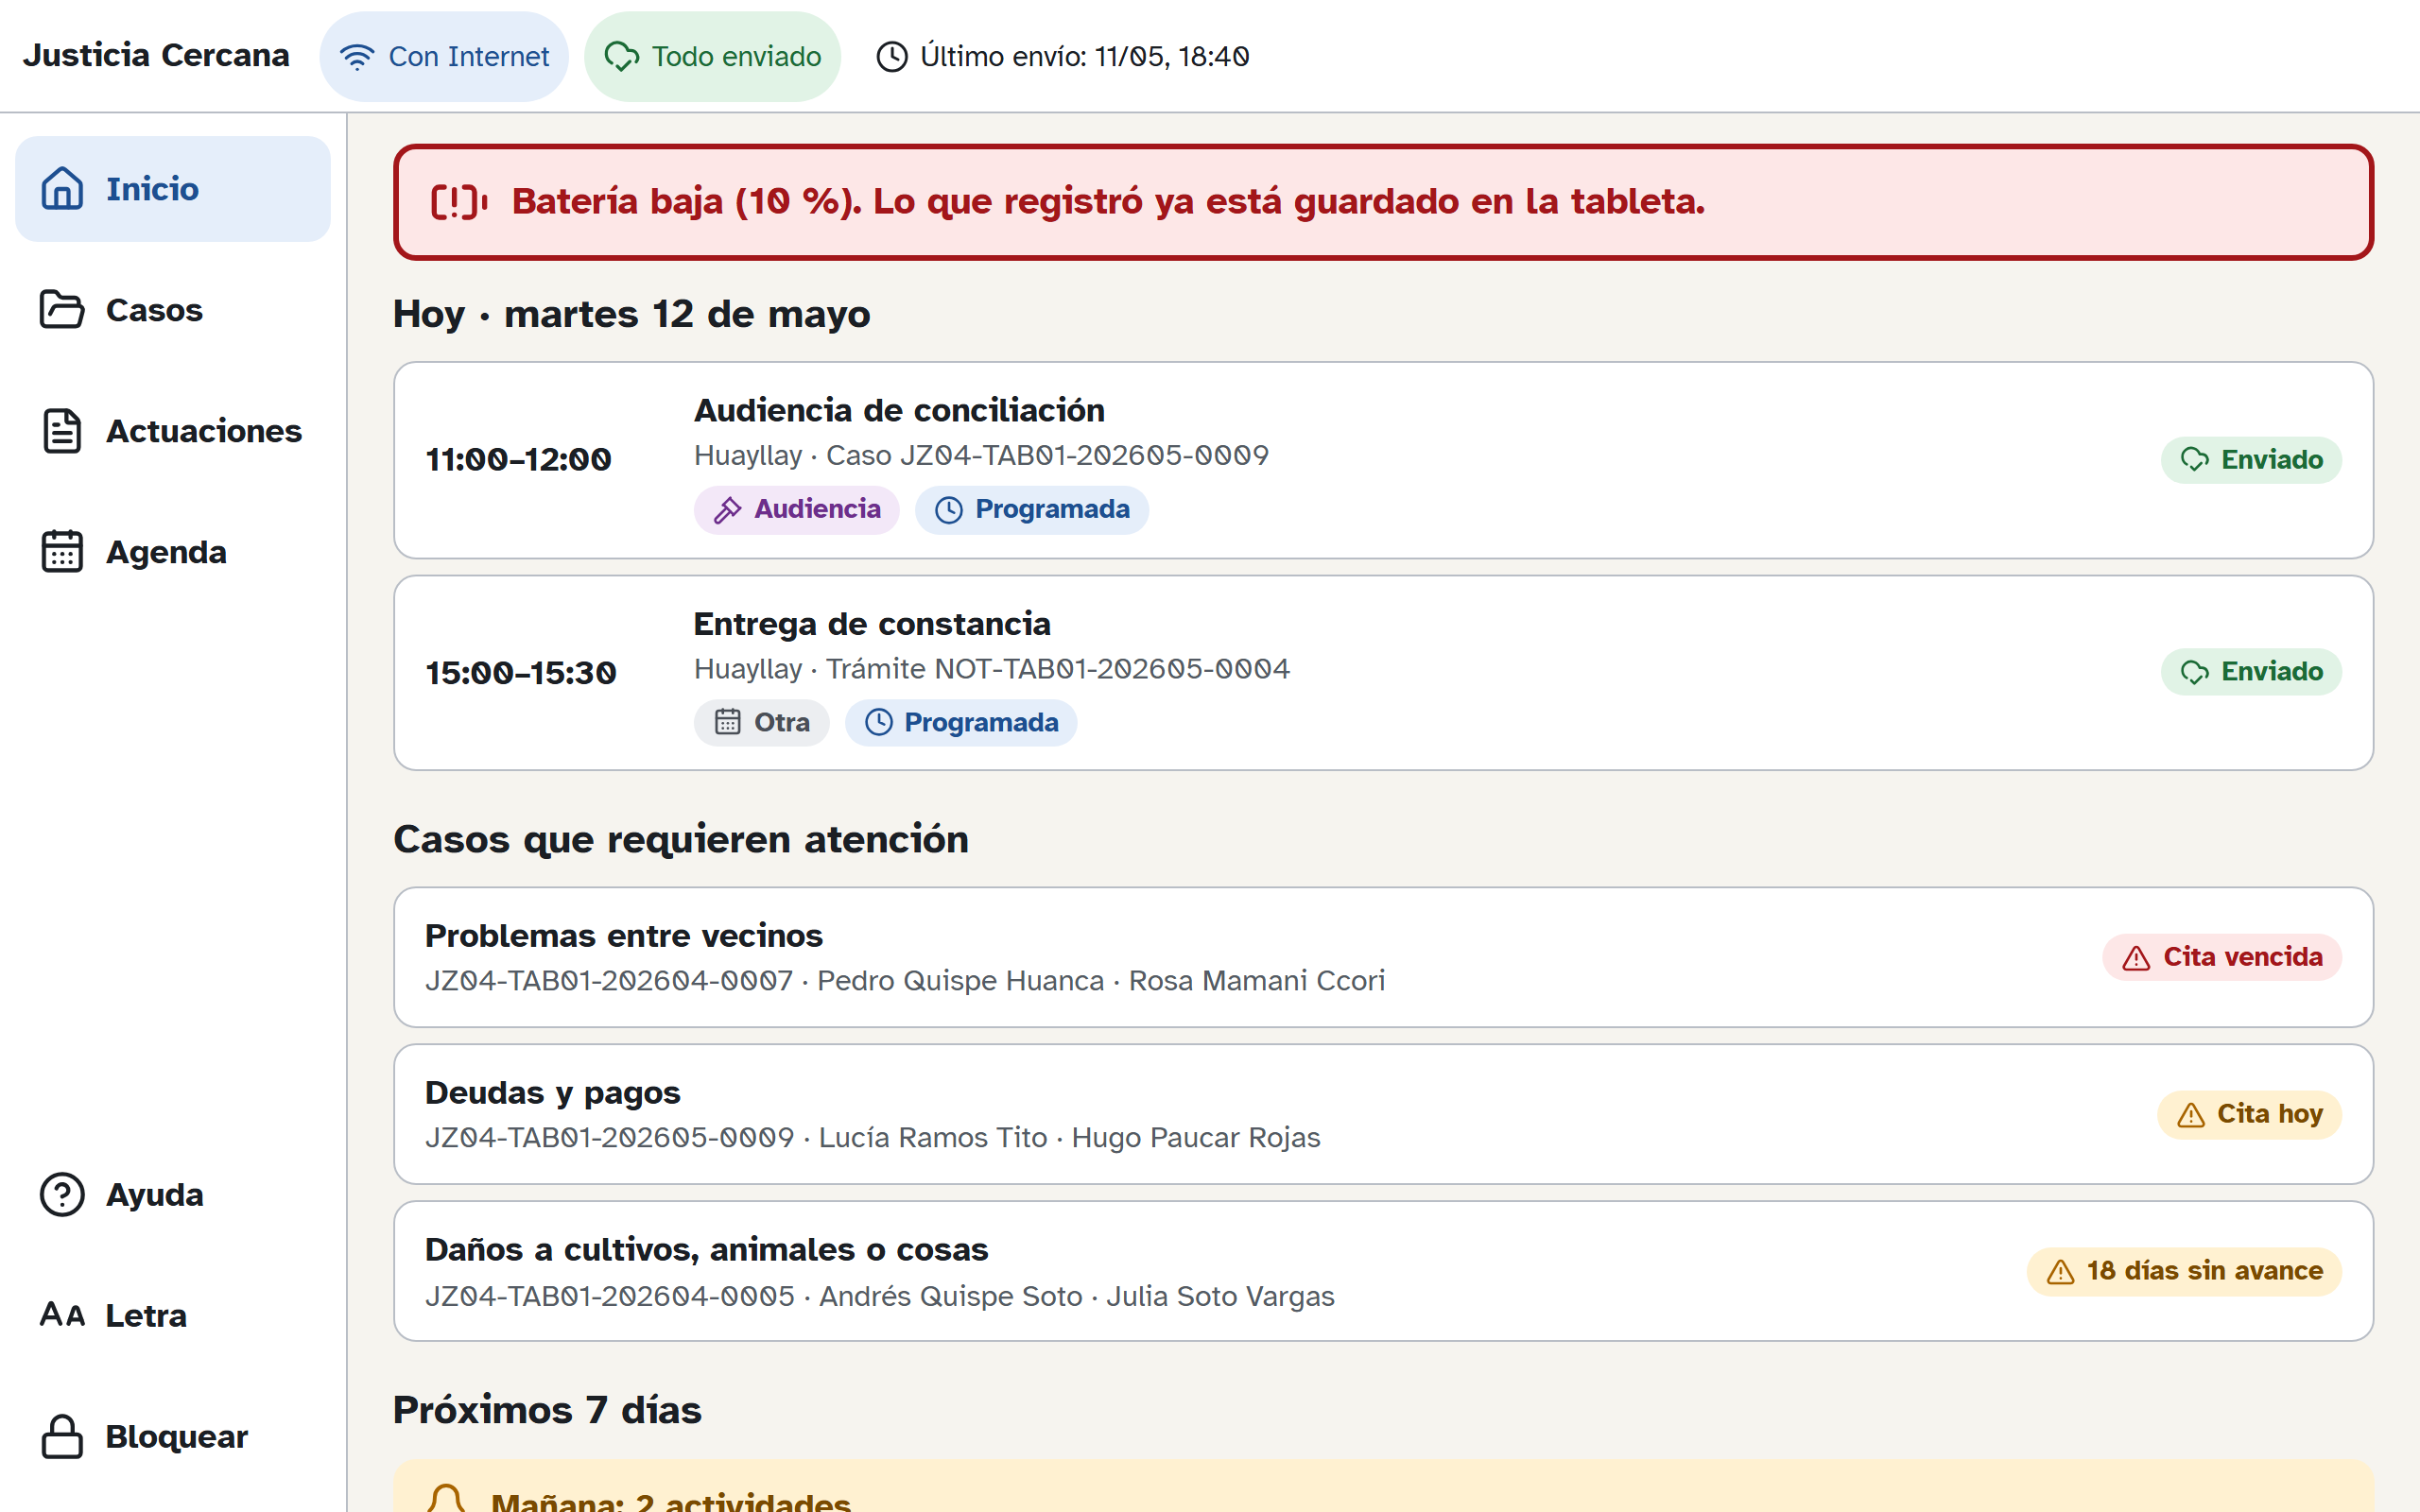
\includegraphics[width=\linewidth]{../../captures/G-13_bateria-10.png}\\[-2pt]{\footnotesize\raggedright\textbf{P-01.} Batería 10 \%: aviso más visible \emph{(Factores humanos y dispositivo)}\par}\end{minipage}\par\vspace{8pt}\noindent
\begin{minipage}[t]{0.49\textwidth}\centering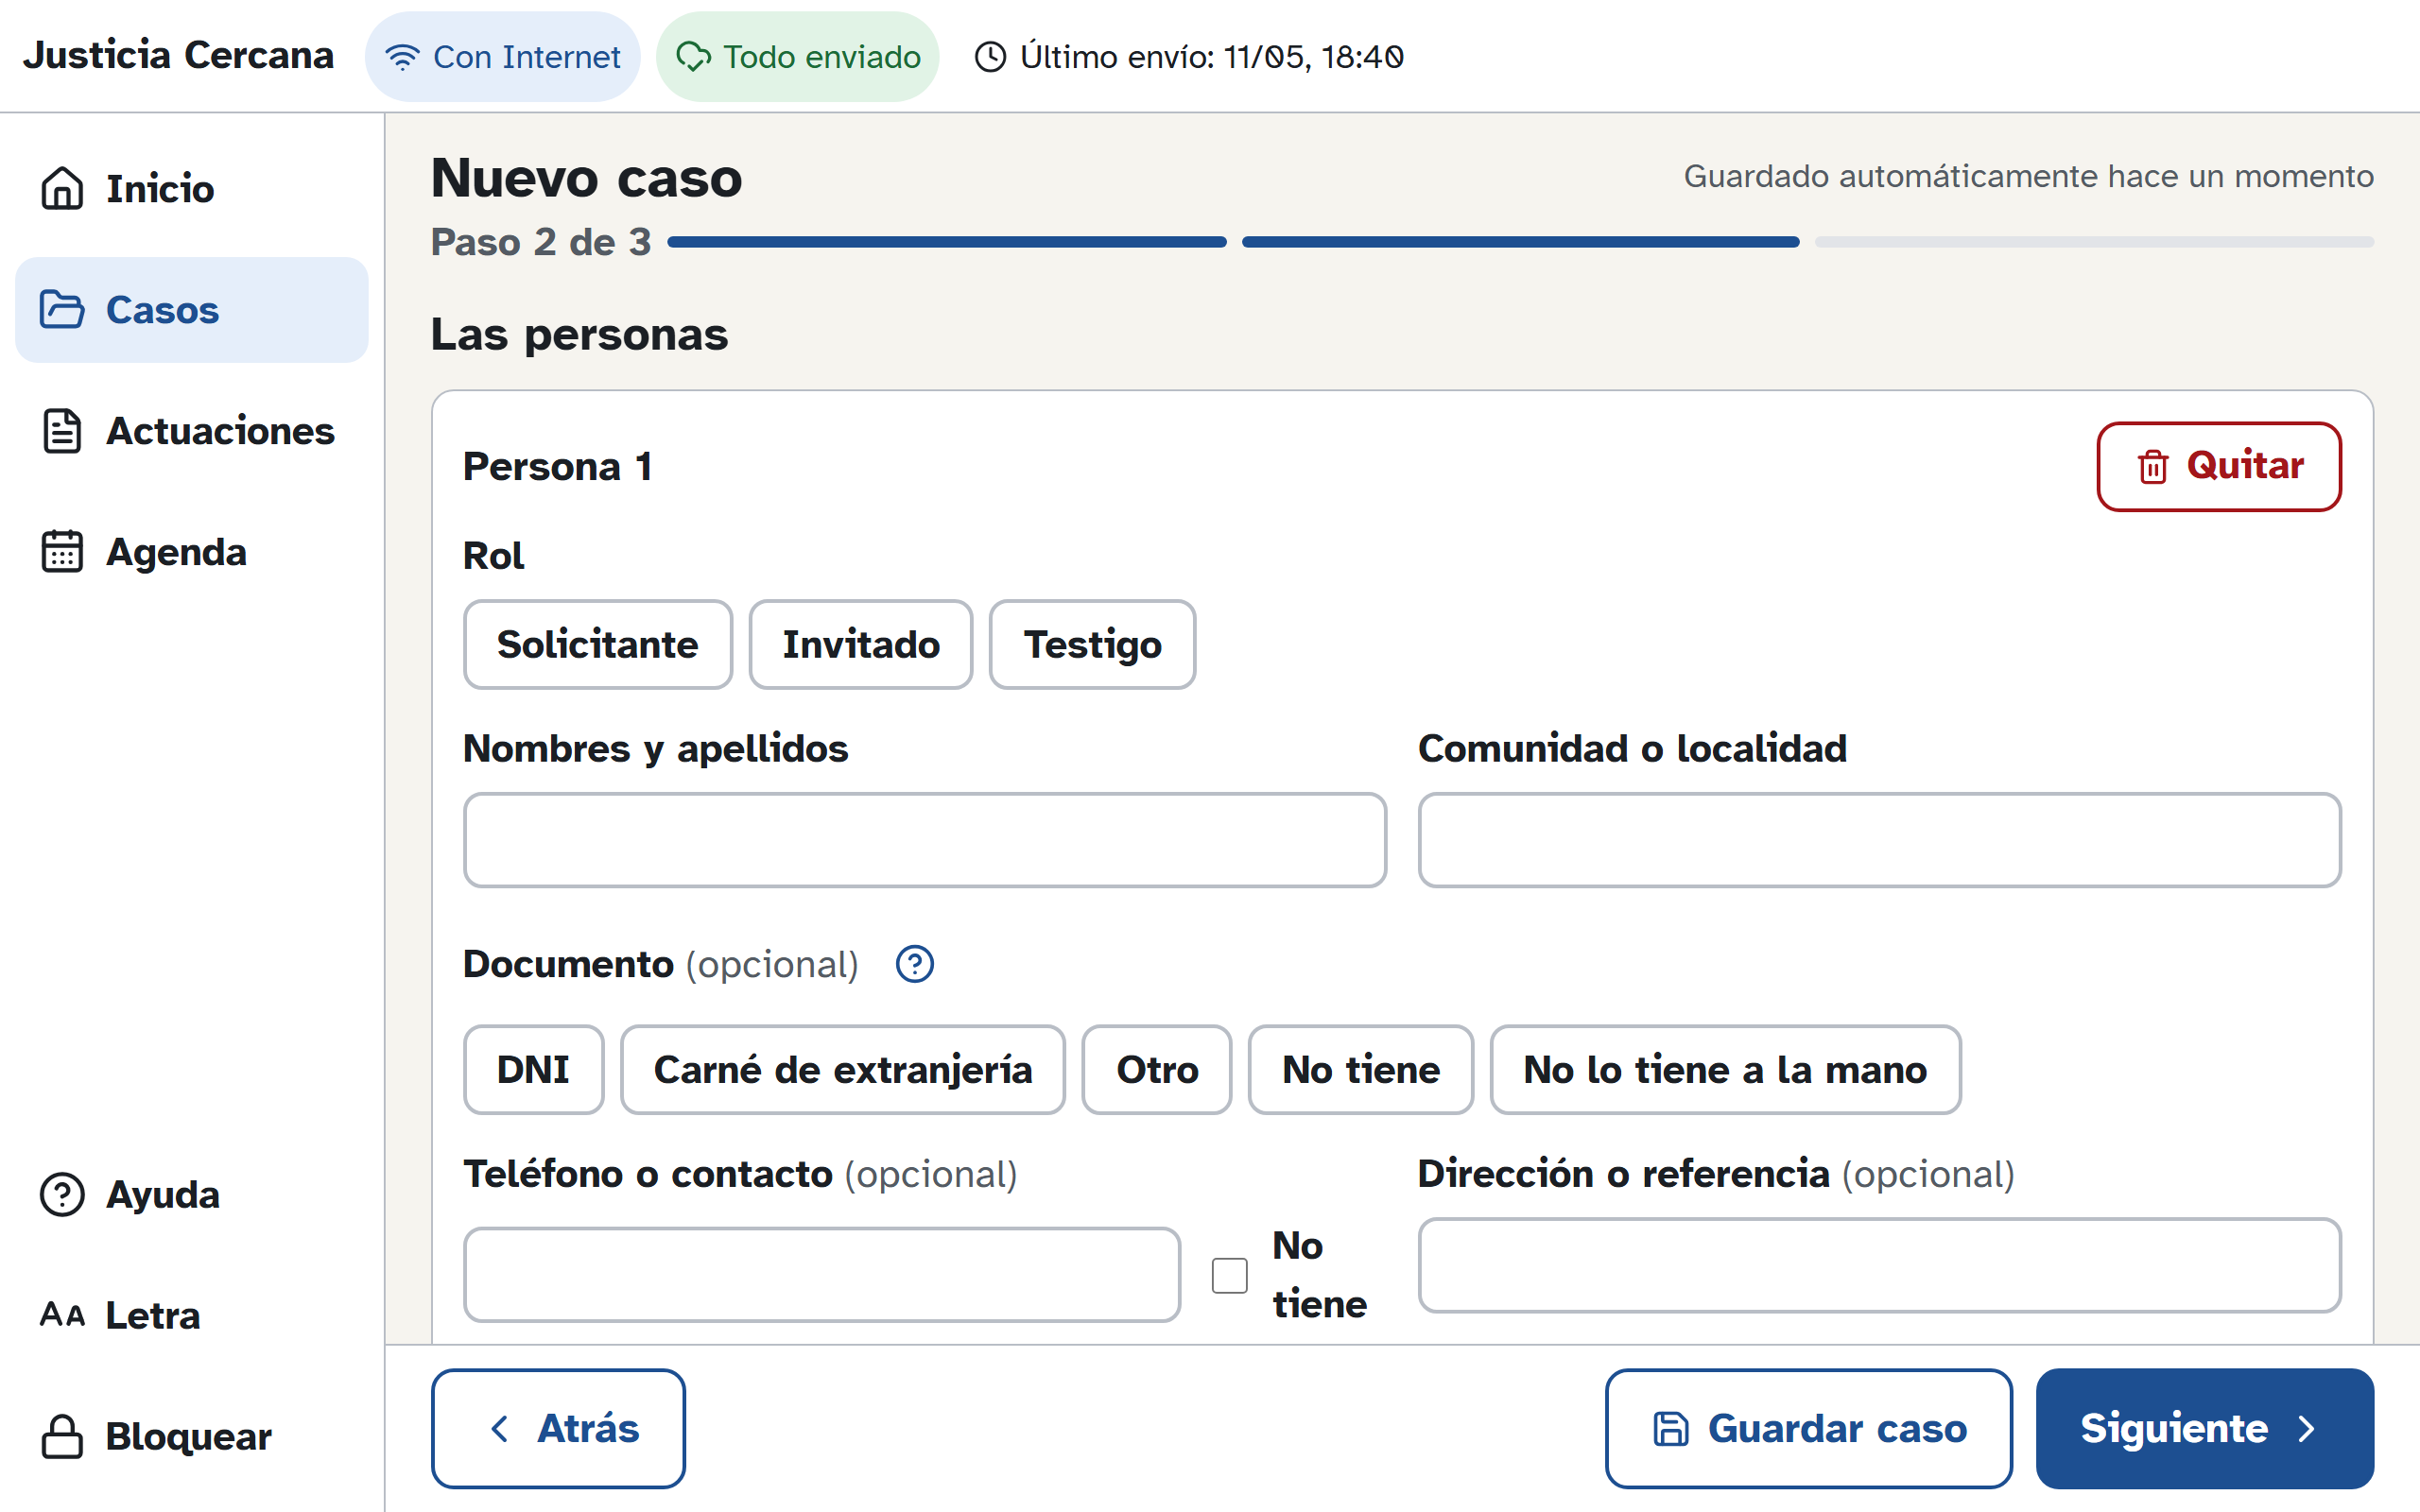
\includegraphics[width=\linewidth]{../../captures/G-14_letra-grande-formulario.png}\\[-2pt]{\footnotesize\raggedright\textbf{P-03.} Formulario en letra Grande (21 px) sin romper el diseño \emph{(Factores humanos y dispositivo)}\par}\end{minipage}\hfill
\begin{minipage}[t]{0.49\textwidth}\centering
\includegraphics[width=\linewidth]{../../captures/G-15_gire-la-tableta.png}\\[-2pt]{\footnotesize\raggedright\textbf{Global.} ``Gire la tableta para usarla de lado'' en vertical 800×1280 \emph{(Factores humanos y dispositivo)}\par}\end{minipage}\par\vspace{8pt}\noindent
\begin{minipage}[t]{0.49\textwidth}\centering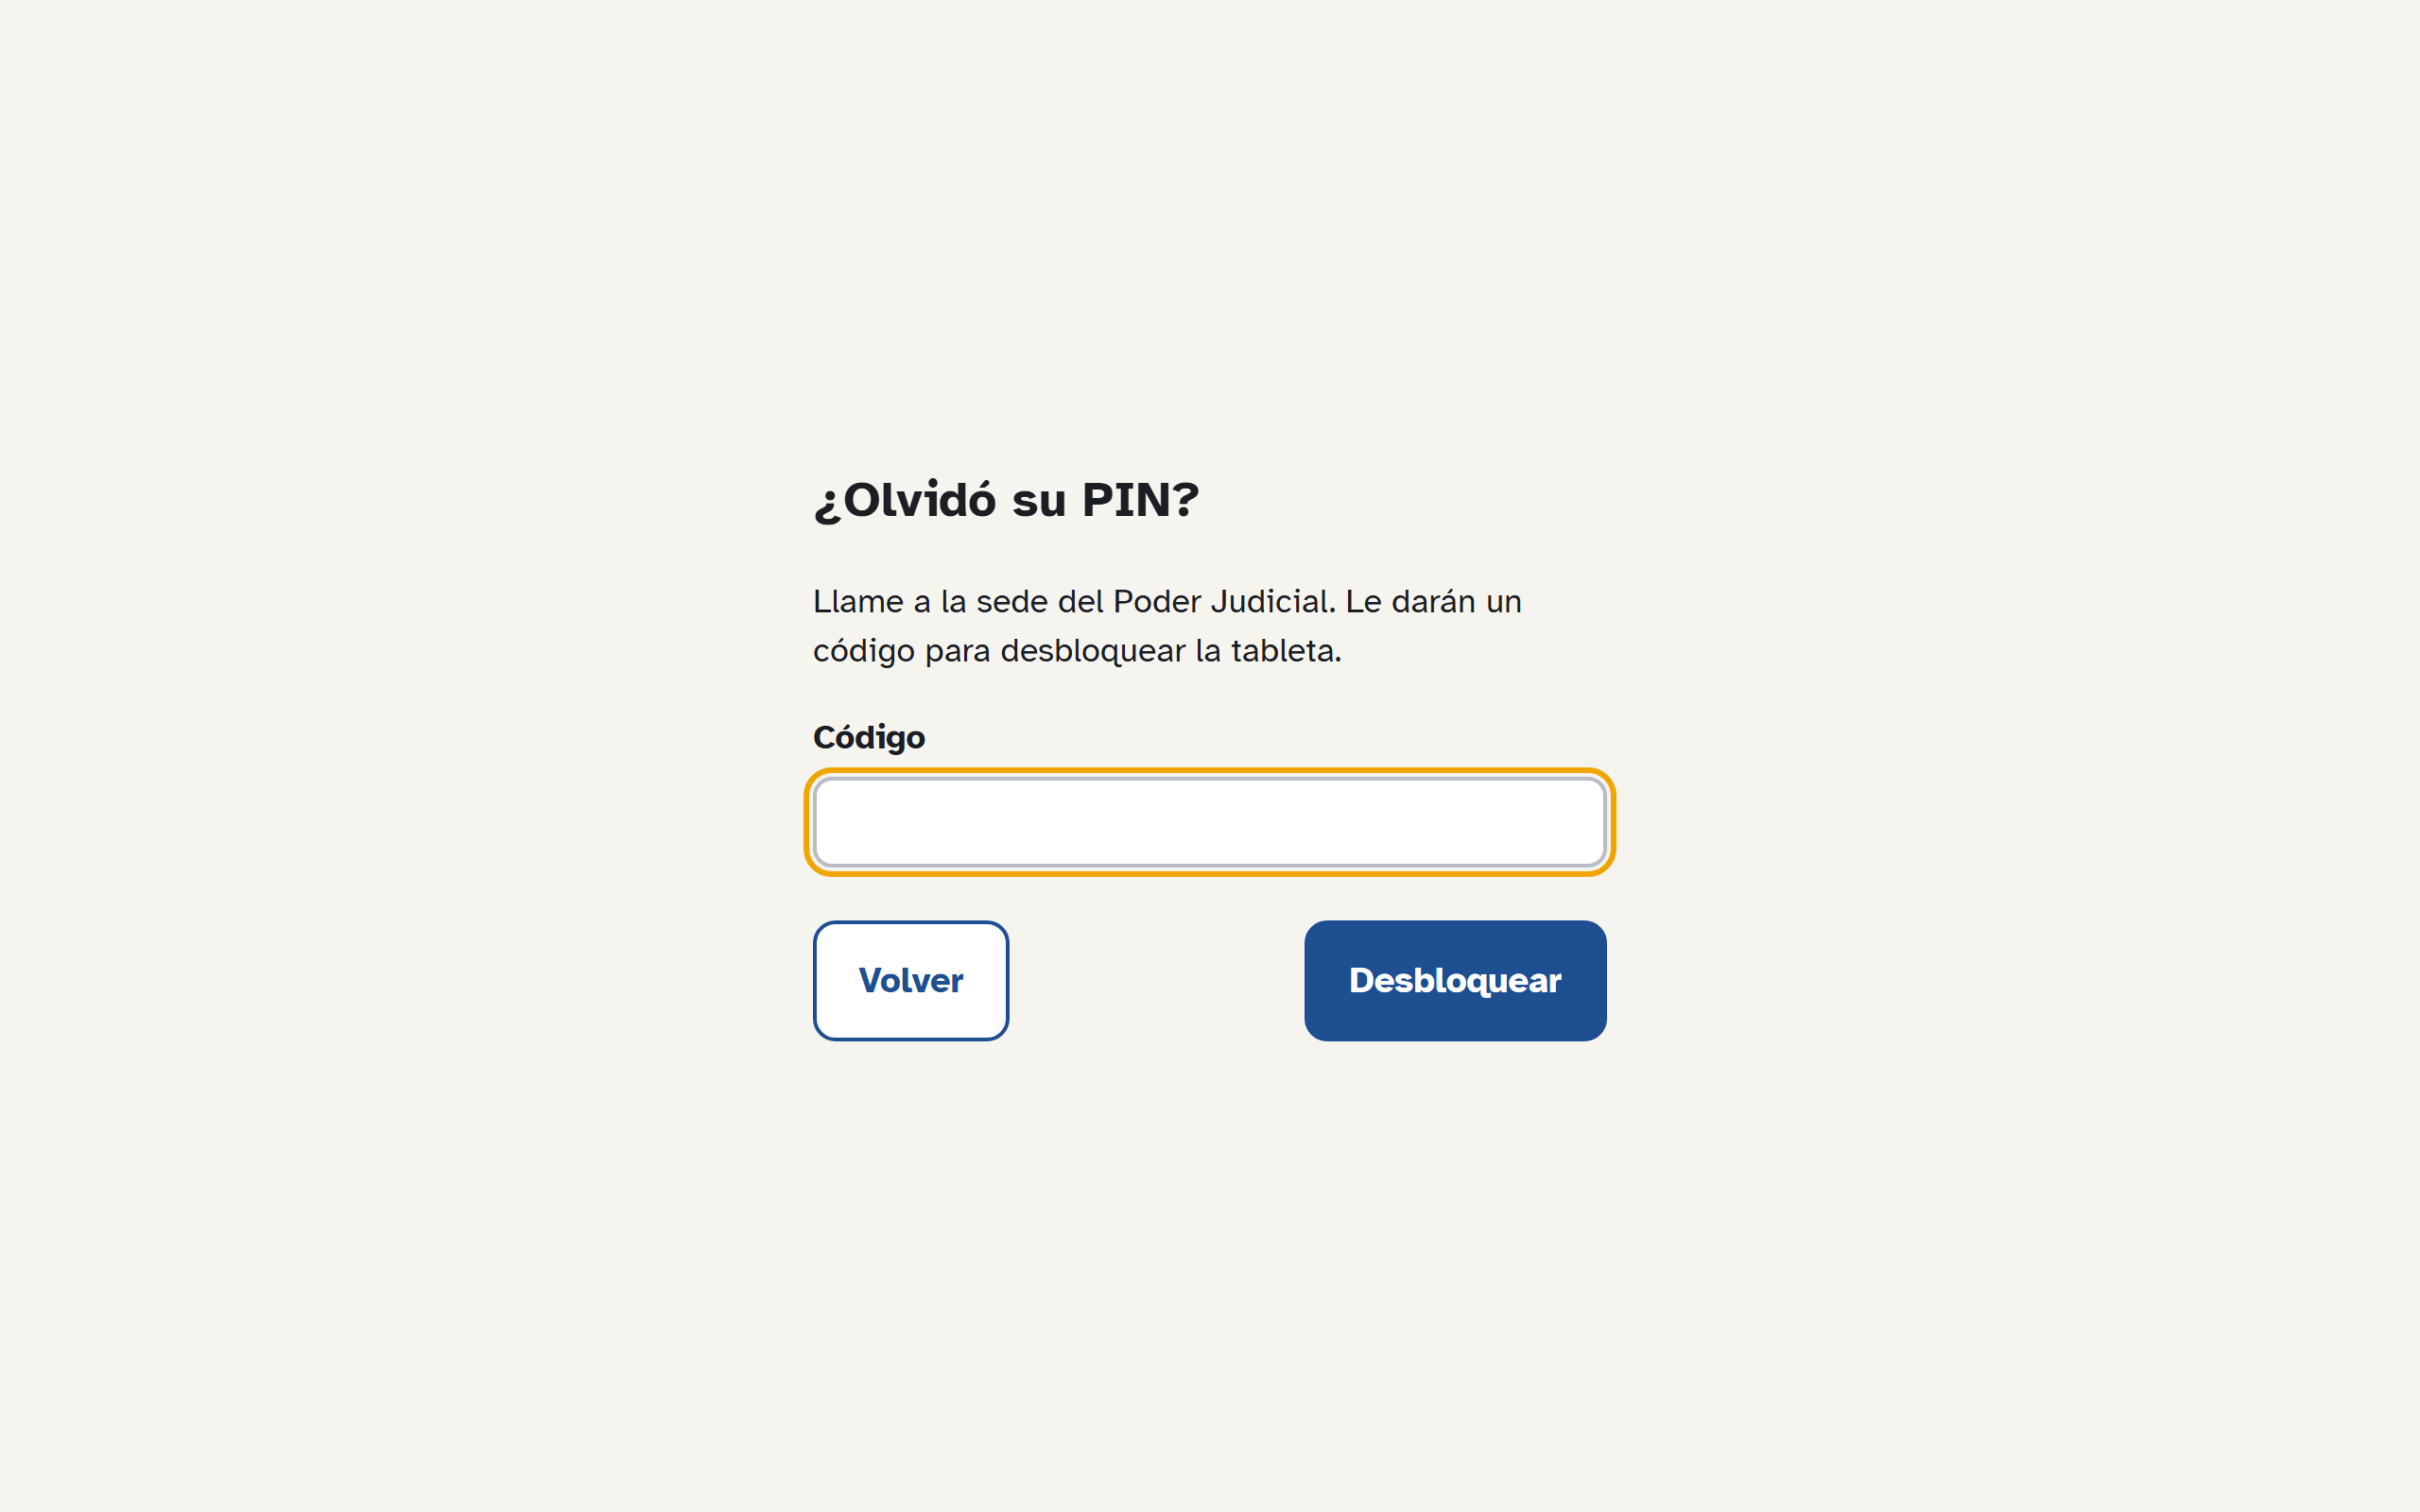
\includegraphics[width=\linewidth]{../../captures/P-00_olvido-pin.png}\\[-2pt]{\footnotesize\raggedright\textbf{P-00.} ``¿Olvidó su PIN?'' con explicación y campo para el código de la sede \emph{(Principios de diseño y heurísticas)}\par}\end{minipage}\hfill
\begin{minipage}[t]{0.49\textwidth}\centering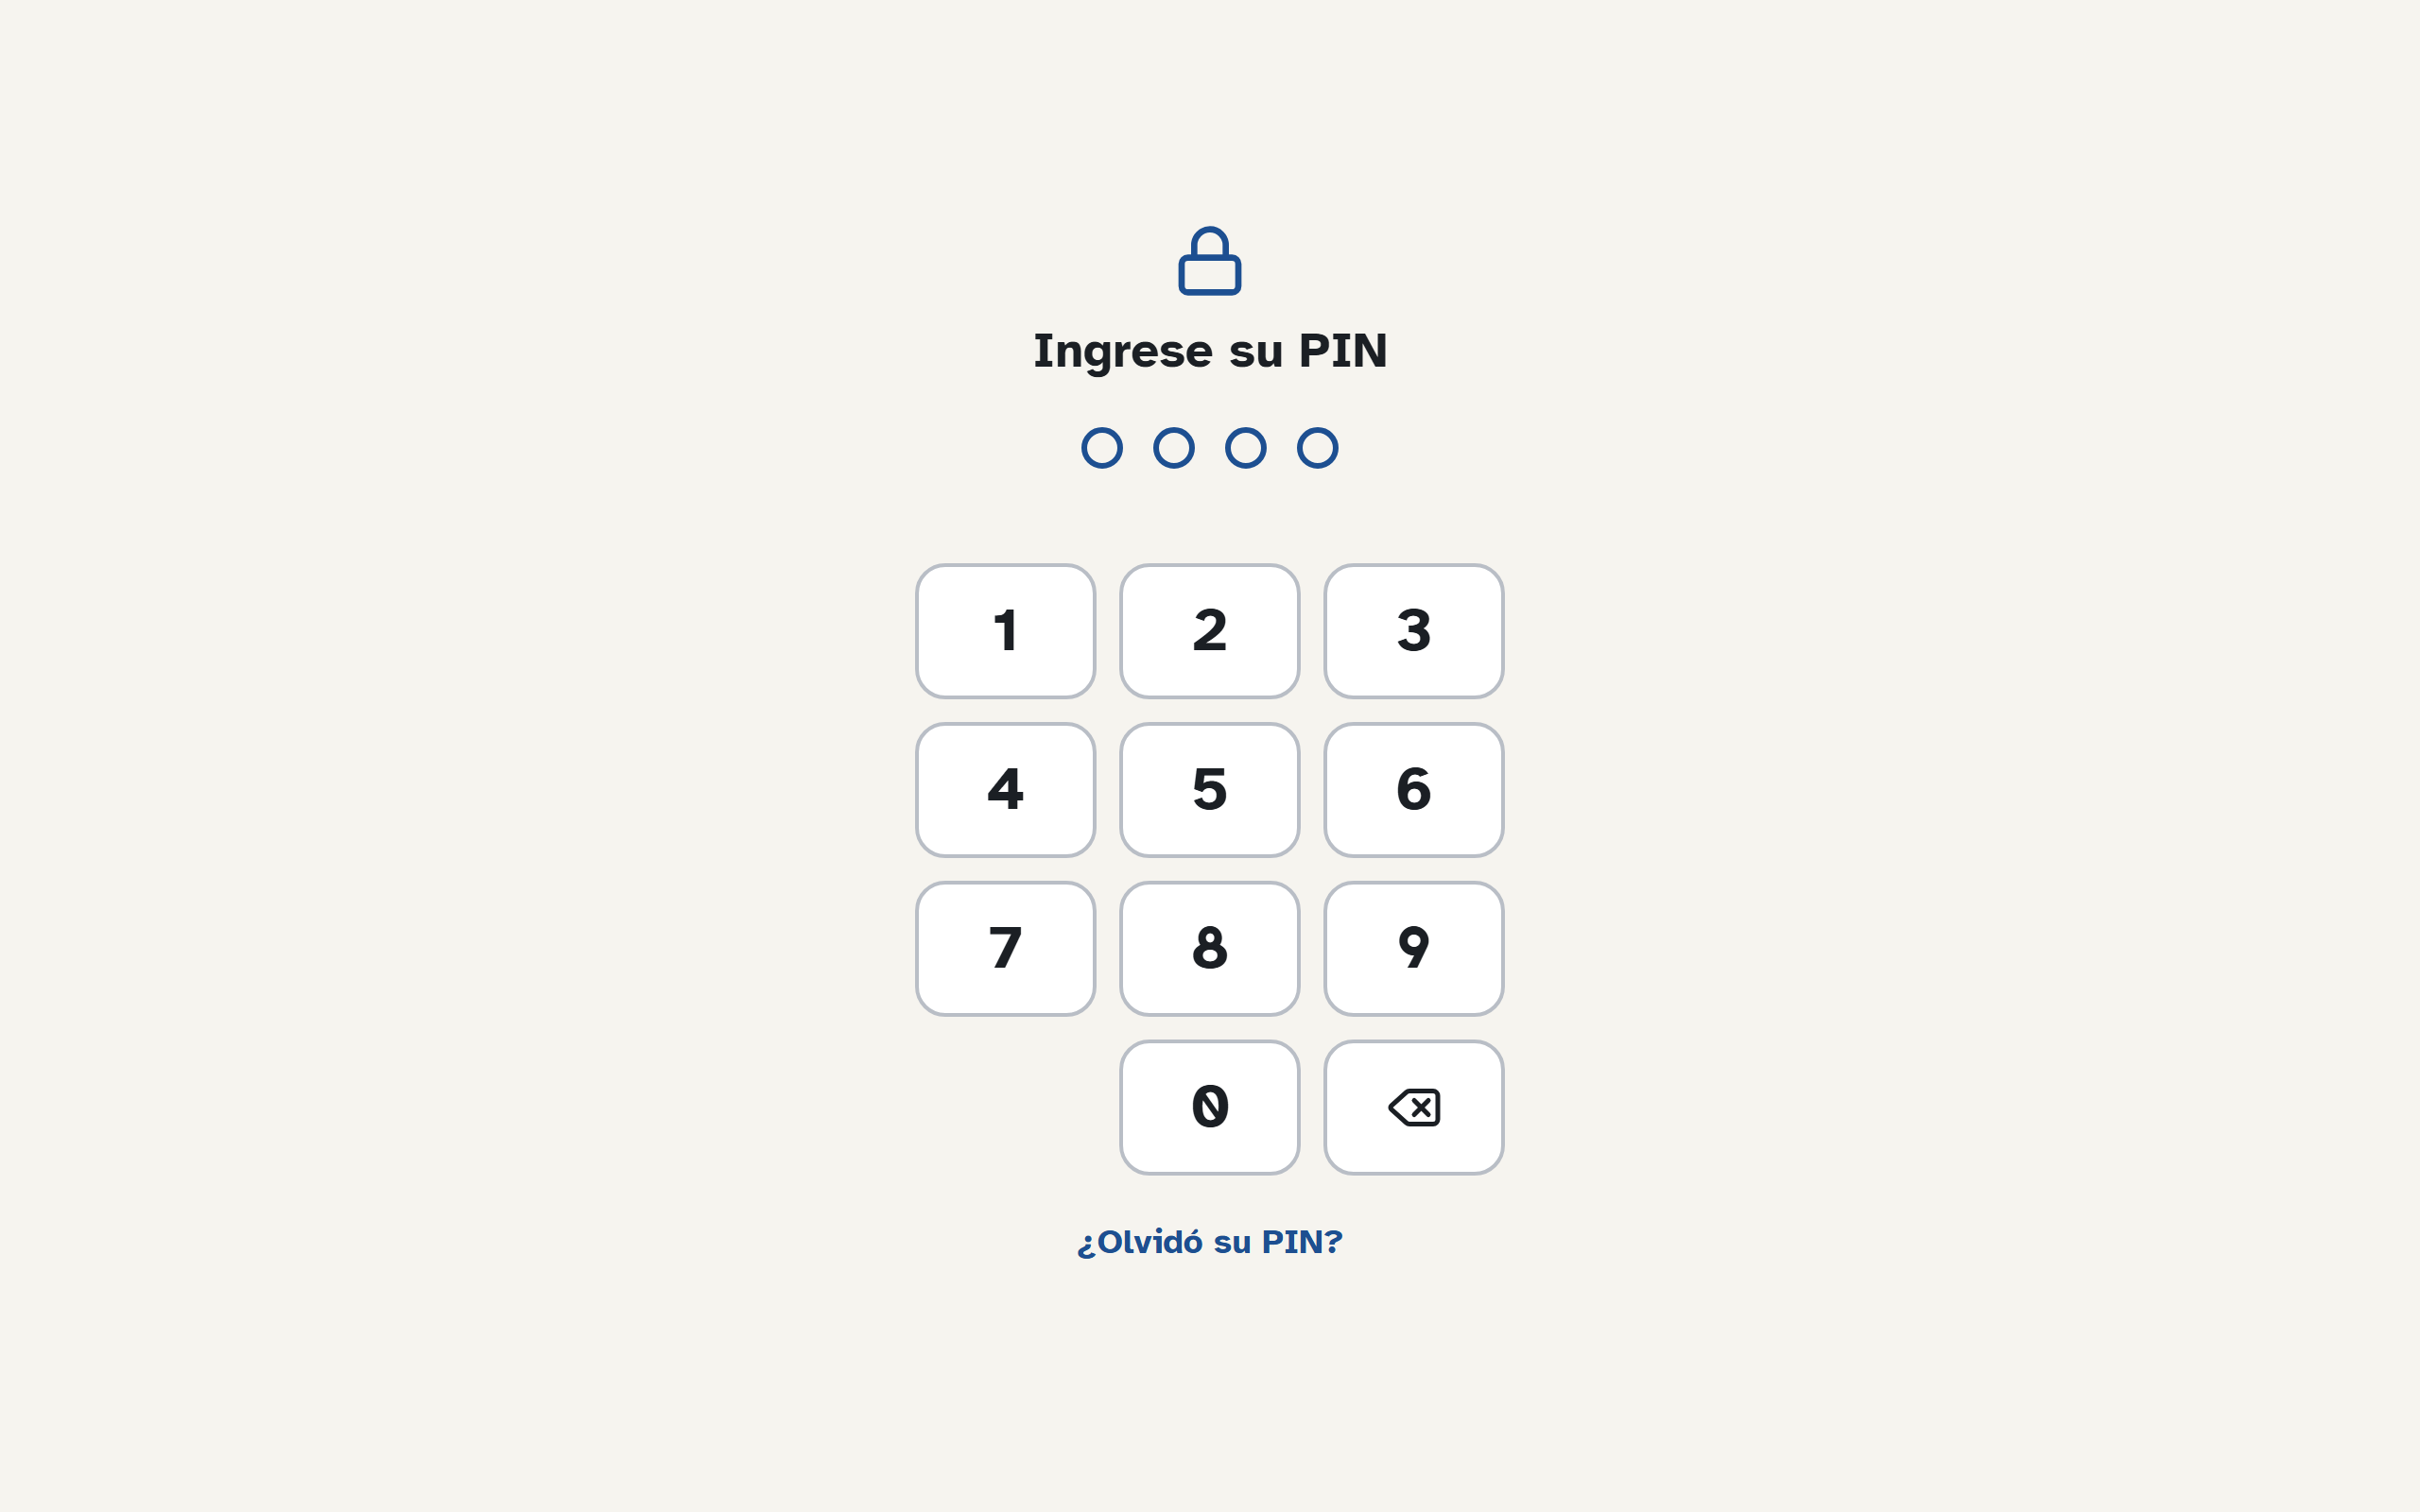
\includegraphics[width=\linewidth]{../../captures/P-00_pin.png}\\[-2pt]{\footnotesize\raggedright\textbf{P-00.} Ingreso con PIN: teclado numérico grande, sin patrón gestual \emph{(Factores humanos y dispositivo)}\par}\end{minipage}\par\vspace{8pt}\noindent
\begin{minipage}[t]{0.49\textwidth}\centering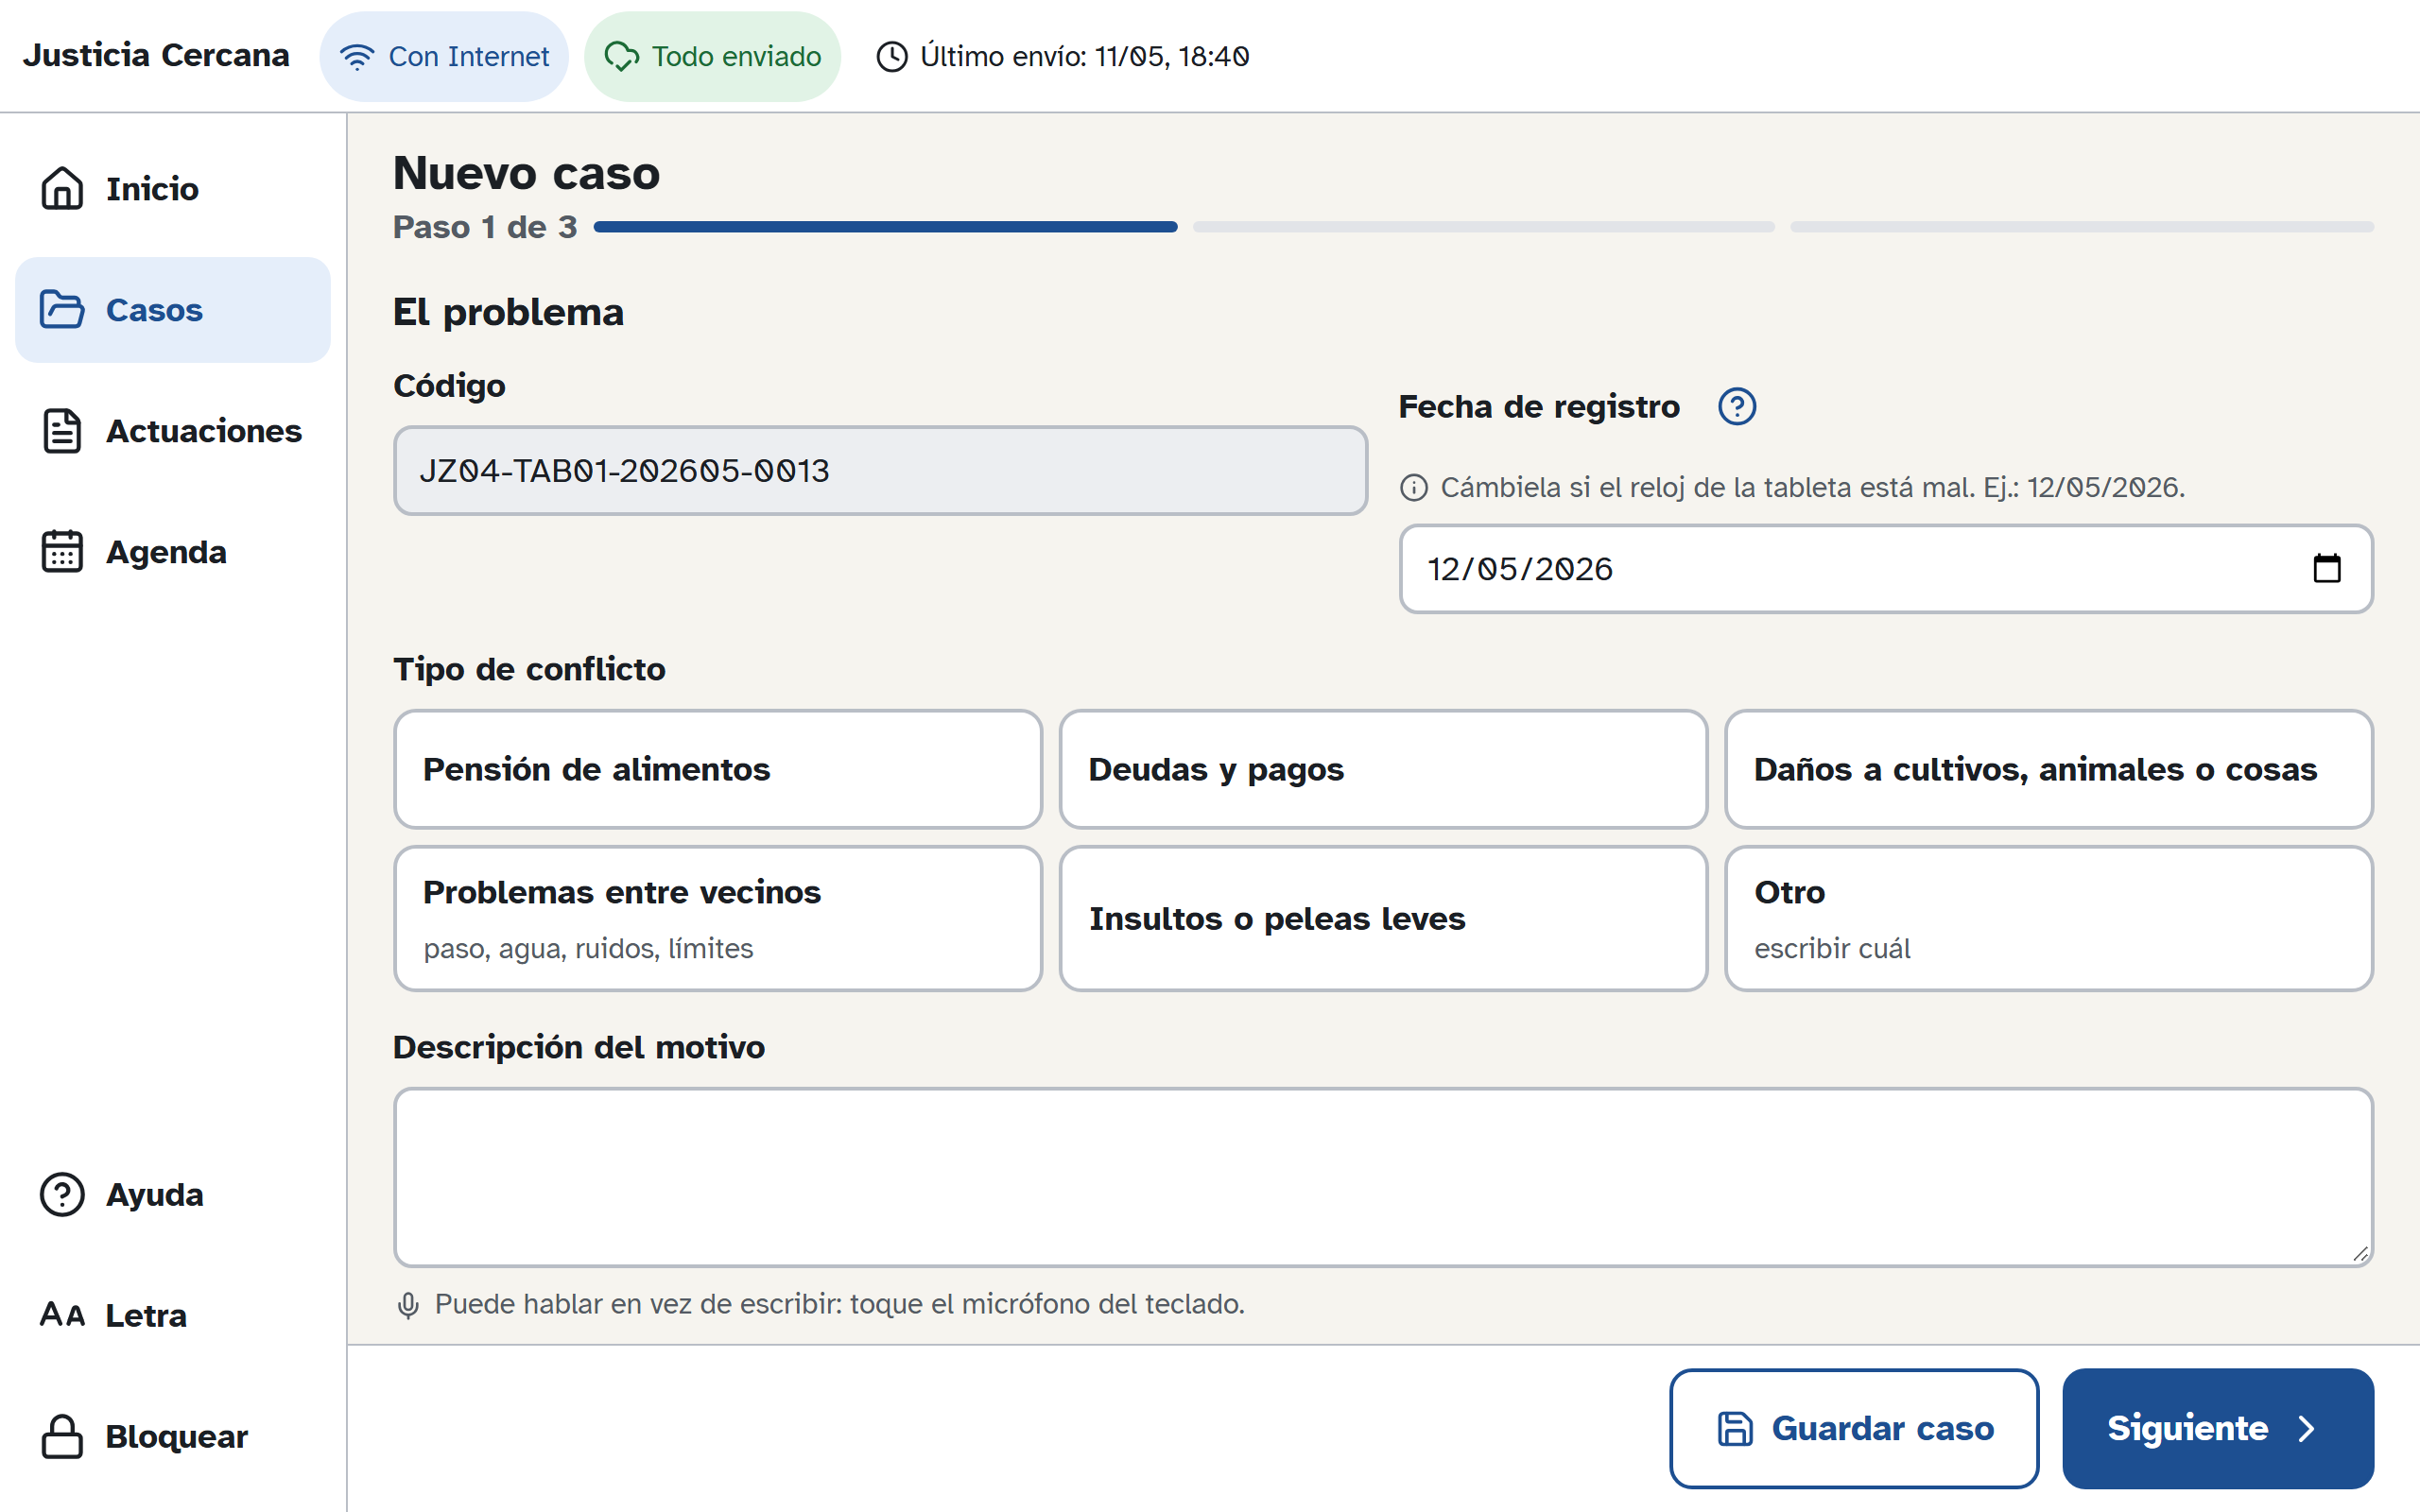
\includegraphics[width=\linewidth]{../../captures/P-00b_ayuda-por-campo.png}\\[-2pt]{\footnotesize\raggedright\textbf{P-00b.} Ayuda por campo (ícono help-circle): una línea con un ejemplo \emph{(Principios de diseño y heurísticas)}\par}\end{minipage}\hfill
\begin{minipage}[t]{0.49\textwidth}\centering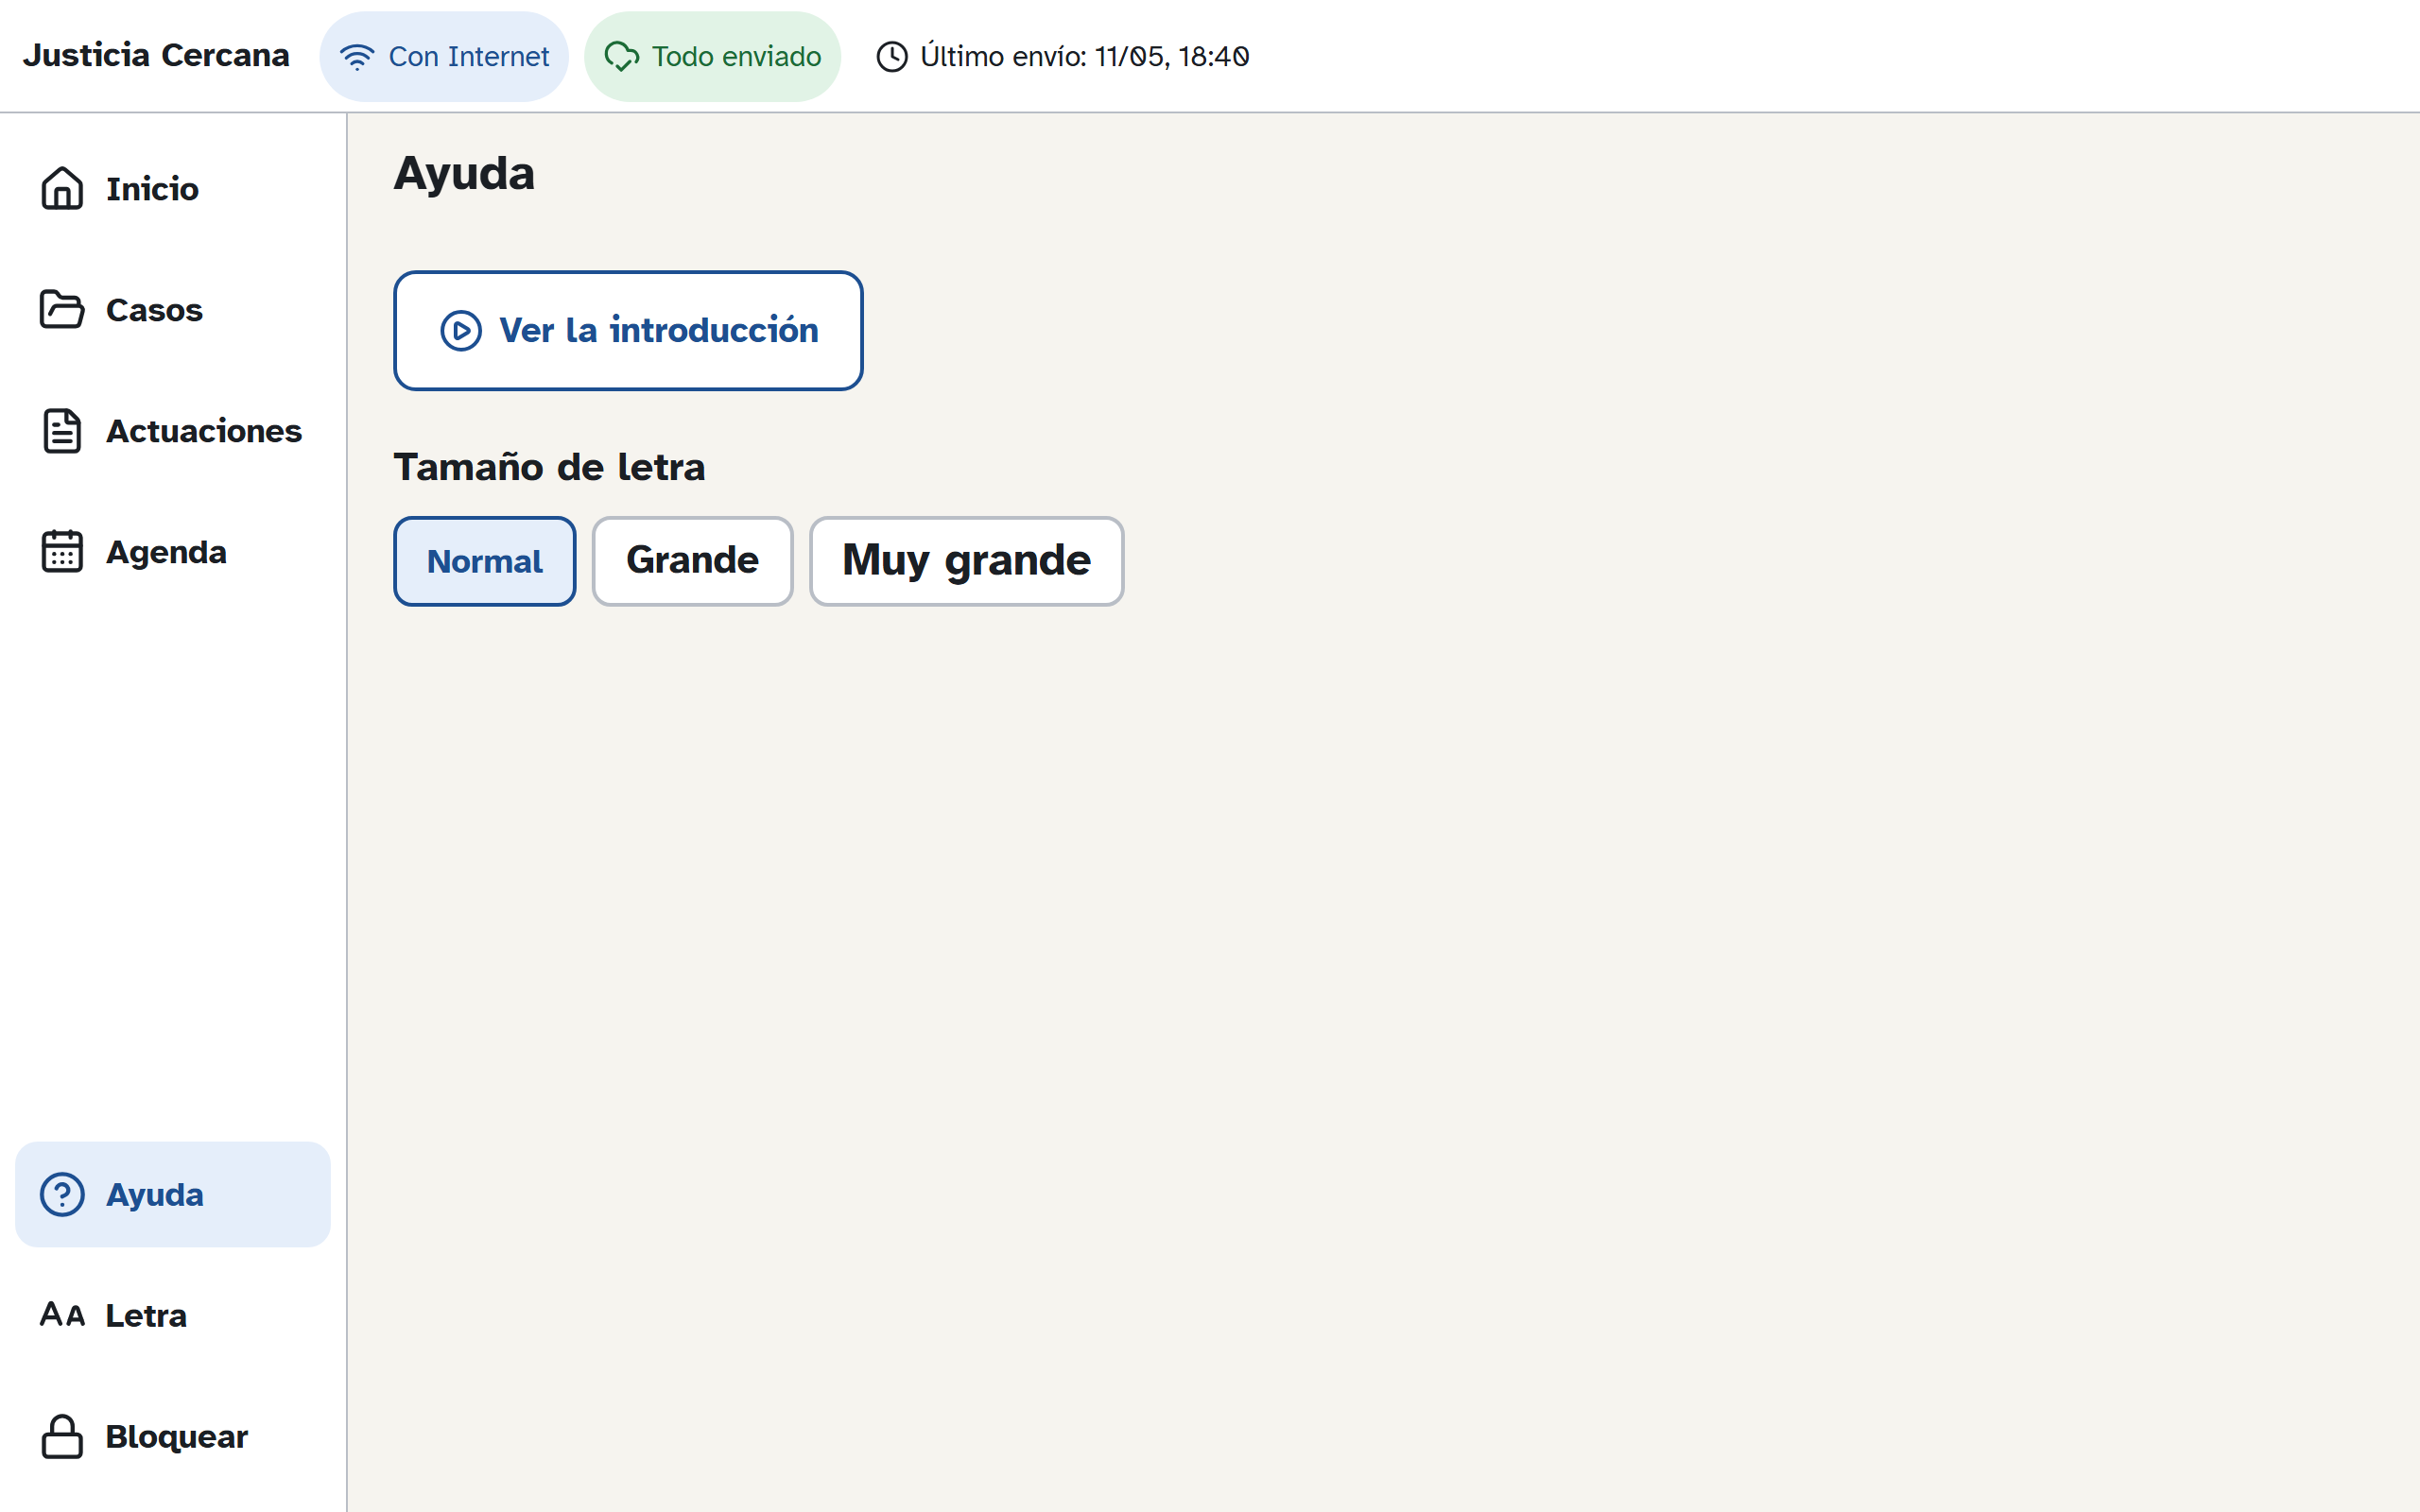
\includegraphics[width=\linewidth]{../../captures/P-00b_ayuda.png}\\[-2pt]{\footnotesize\raggedright\textbf{P-00b.} Ayuda: ver la introducción y tamaño de letra \emph{(Principios de diseño y heurísticas)}\par}\end{minipage}\par\vspace{8pt}\noindent
\begin{minipage}[t]{0.49\textwidth}\centering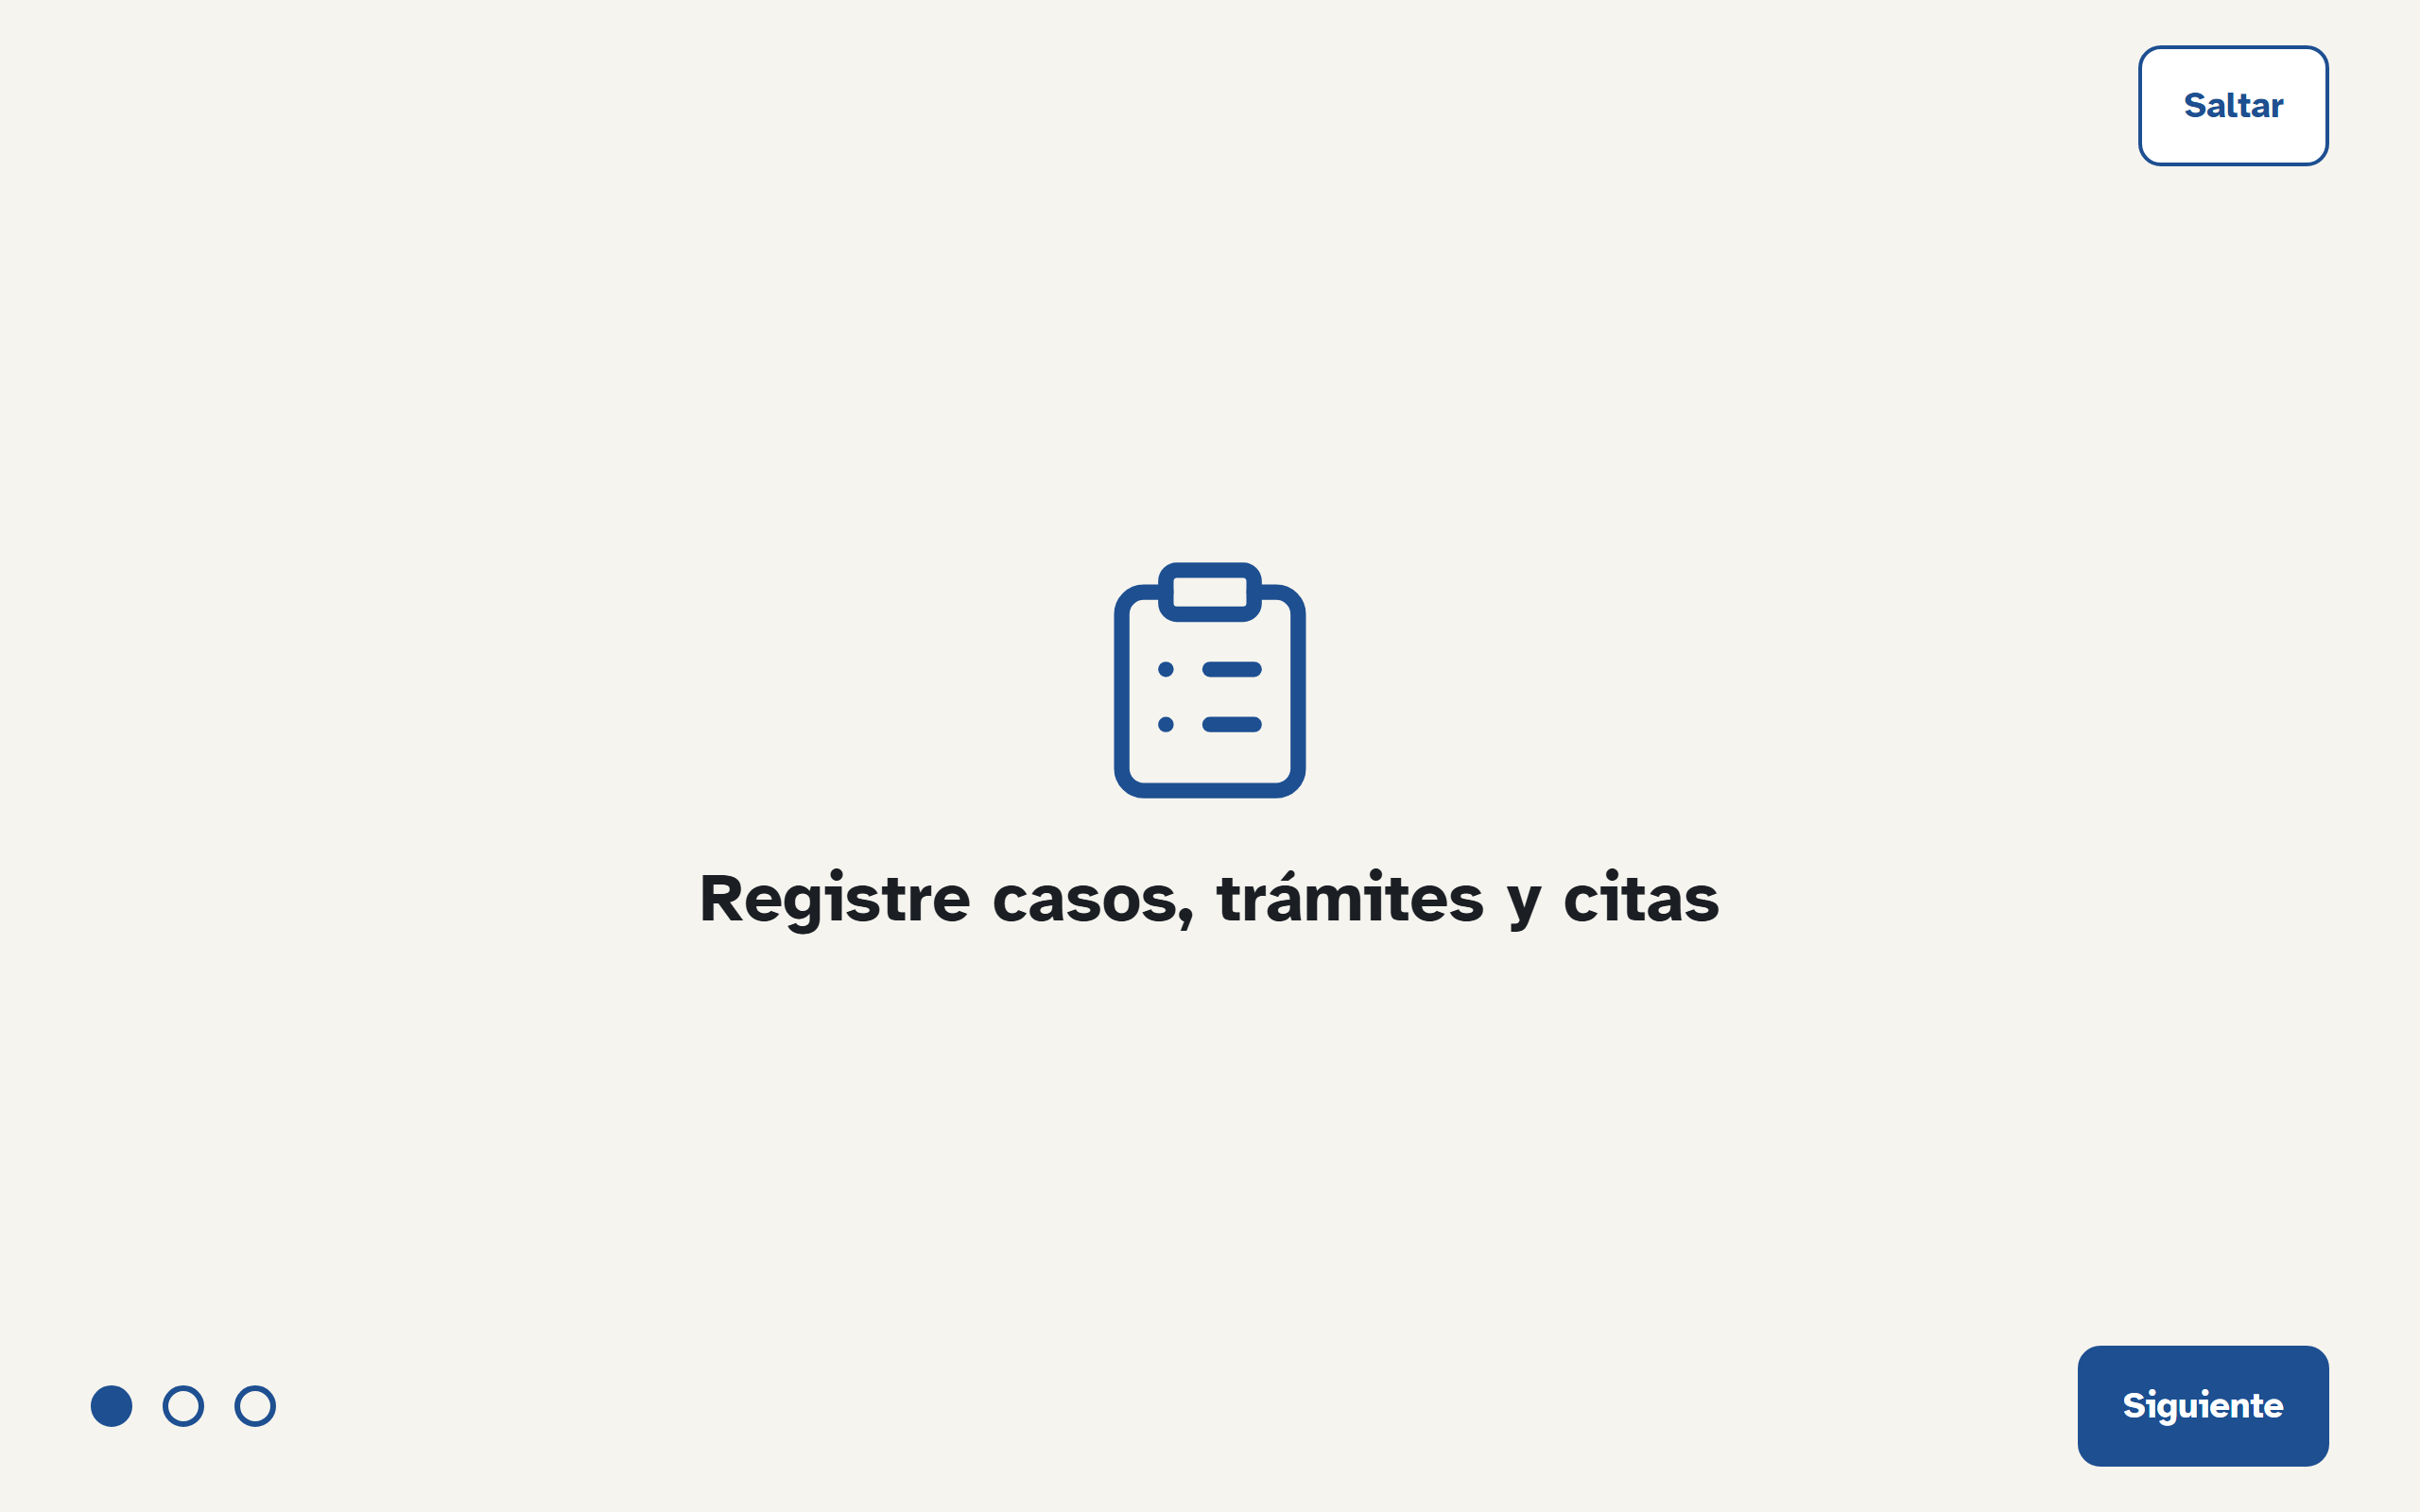
\includegraphics[width=\linewidth]{../../captures/P-00b_introduccion-1.png}\\[-2pt]{\footnotesize\raggedright\textbf{P-00b.} Introducción inicial, pantalla 1 de 3, con [Saltar] visible \emph{(Principios de diseño y heurísticas)}\par}\end{minipage}\hfill
\begin{minipage}[t]{0.49\textwidth}\centering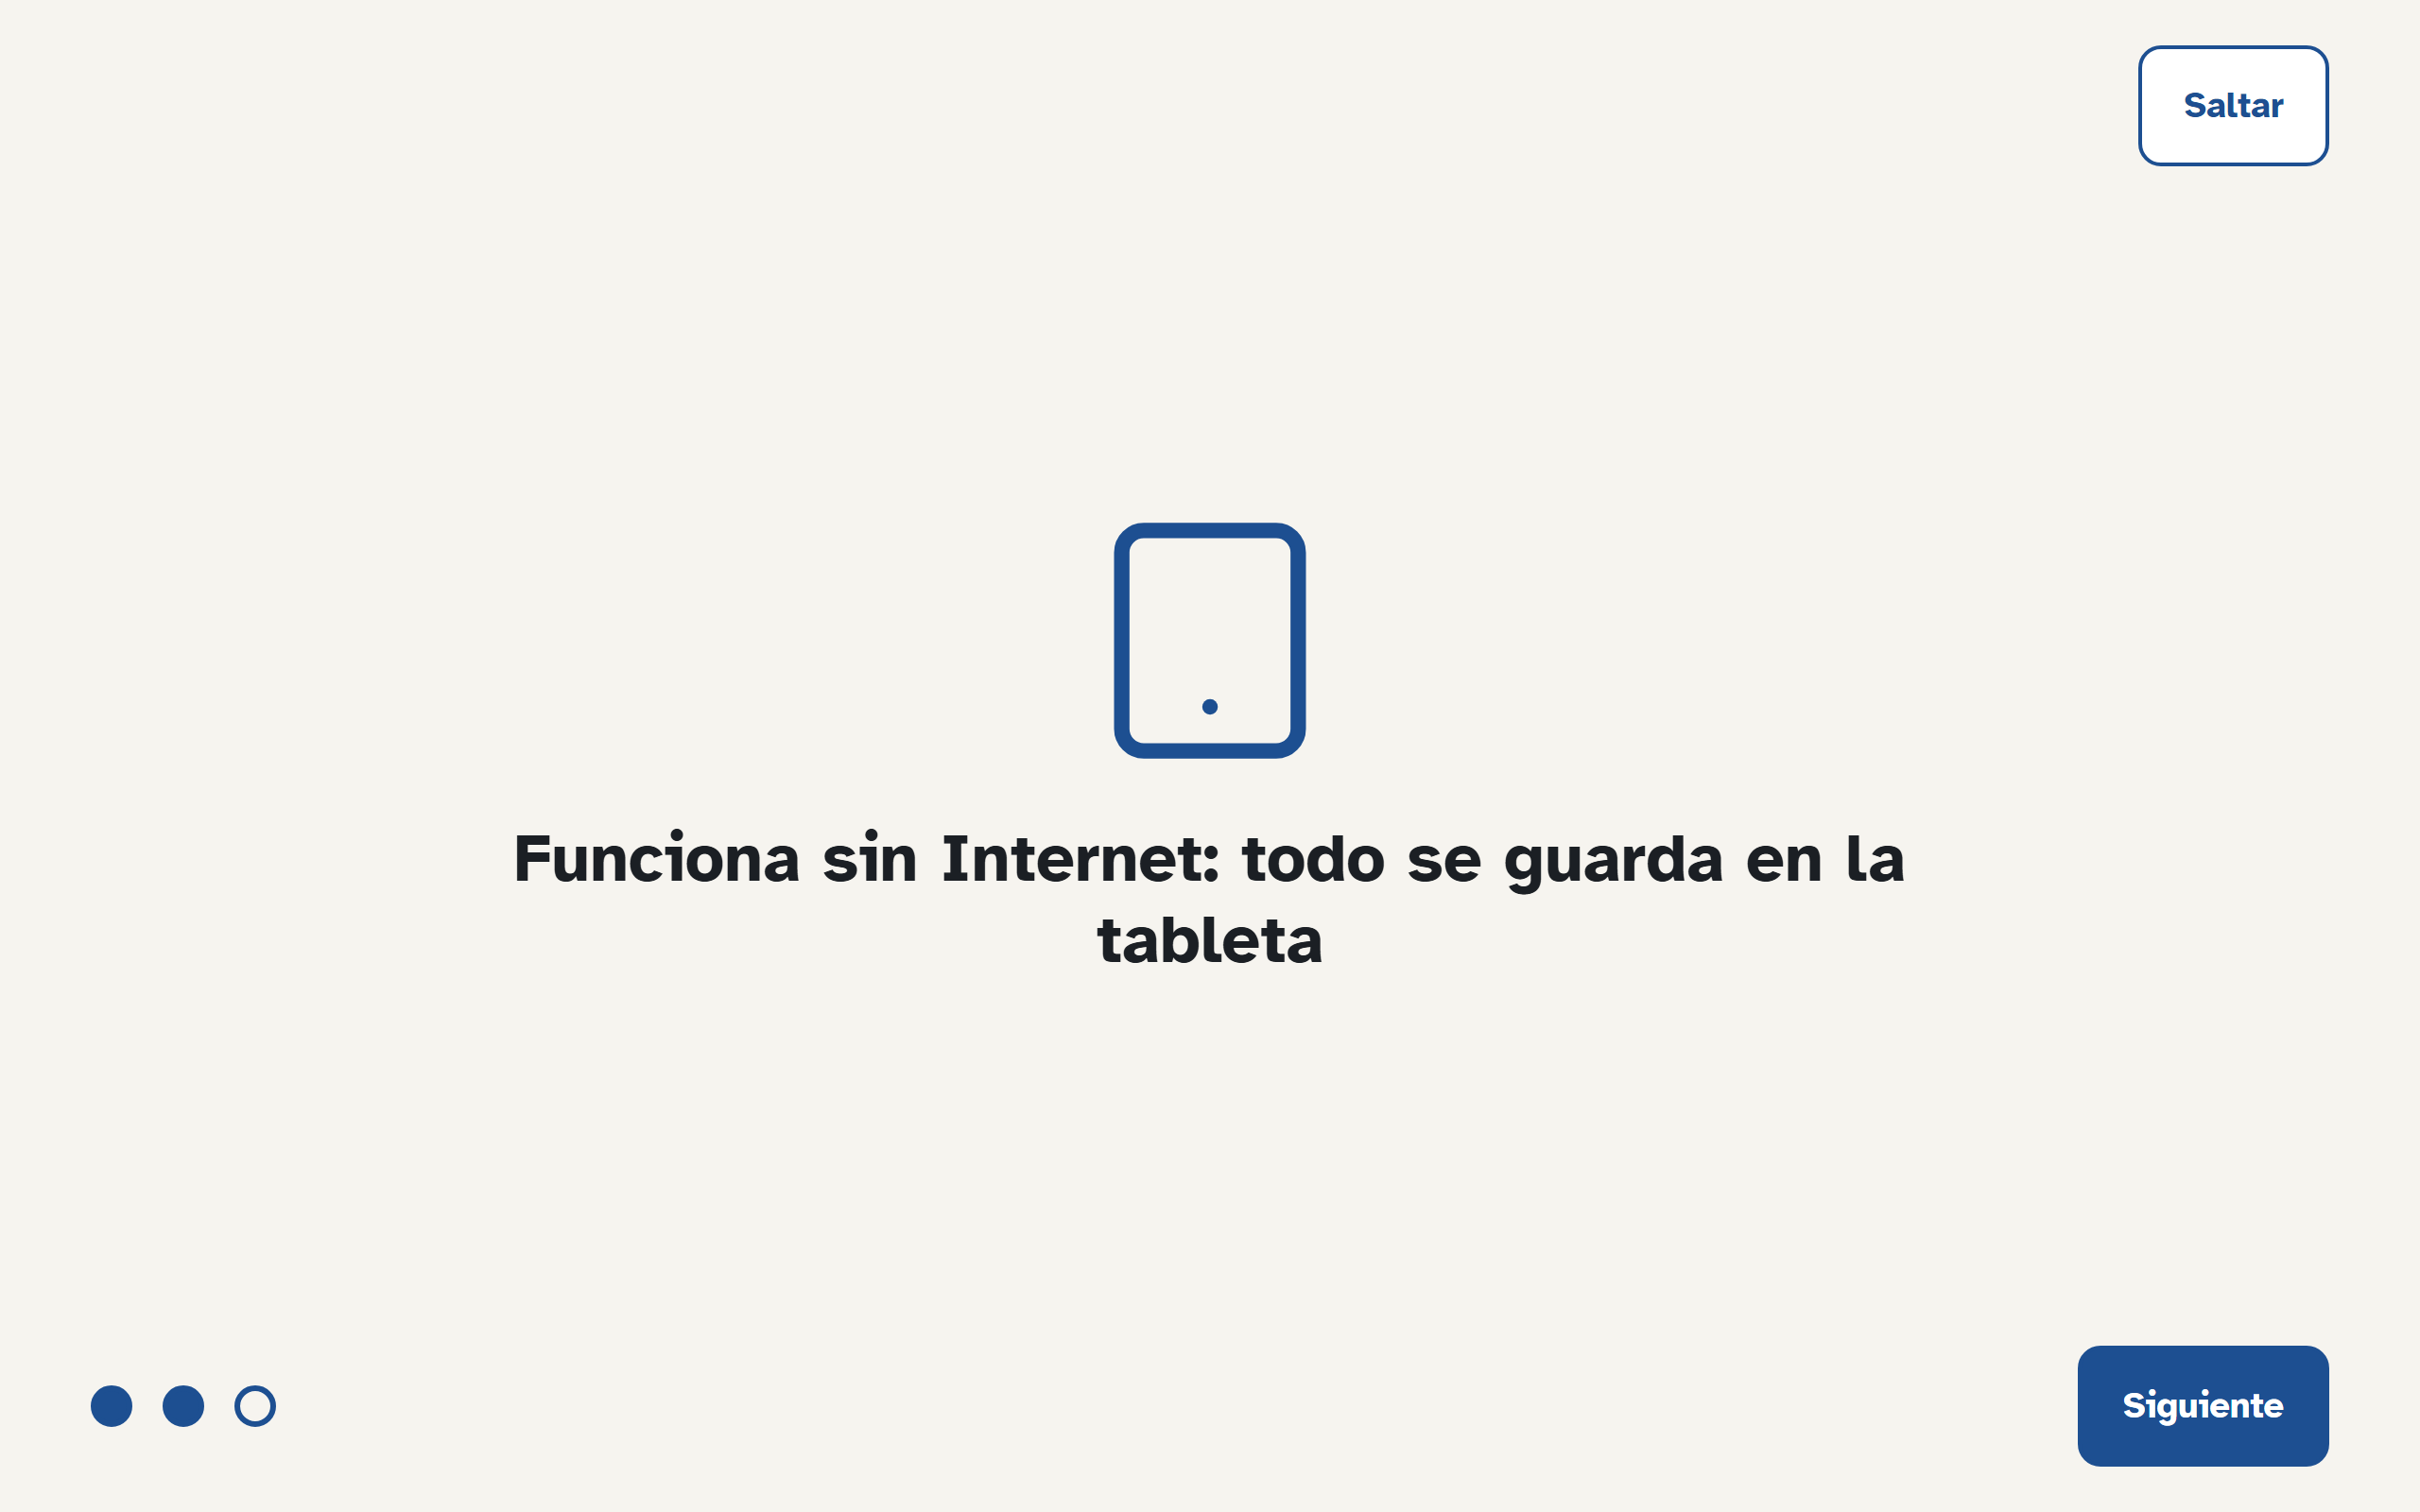
\includegraphics[width=\linewidth]{../../captures/P-00b_introduccion-2.png}\\[-2pt]{\footnotesize\raggedright\textbf{P-00b.} Introducción inicial, pantalla 2 de 3, con [Saltar] visible \emph{(Principios de diseño y heurísticas)}\par}\end{minipage}\par\vspace{8pt}\noindent
\begin{minipage}[t]{0.49\textwidth}\centering
\includegraphics[width=\linewidth]{../../captures/P-00b_introduccion-3.png}\\[-2pt]{\footnotesize\raggedright\textbf{P-00b.} Introducción inicial, pantalla 3 de 3, con [Saltar] visible \emph{(Principios de diseño y heurísticas)}\par}\end{minipage}\hfill
\begin{minipage}[t]{0.49\textwidth}\centering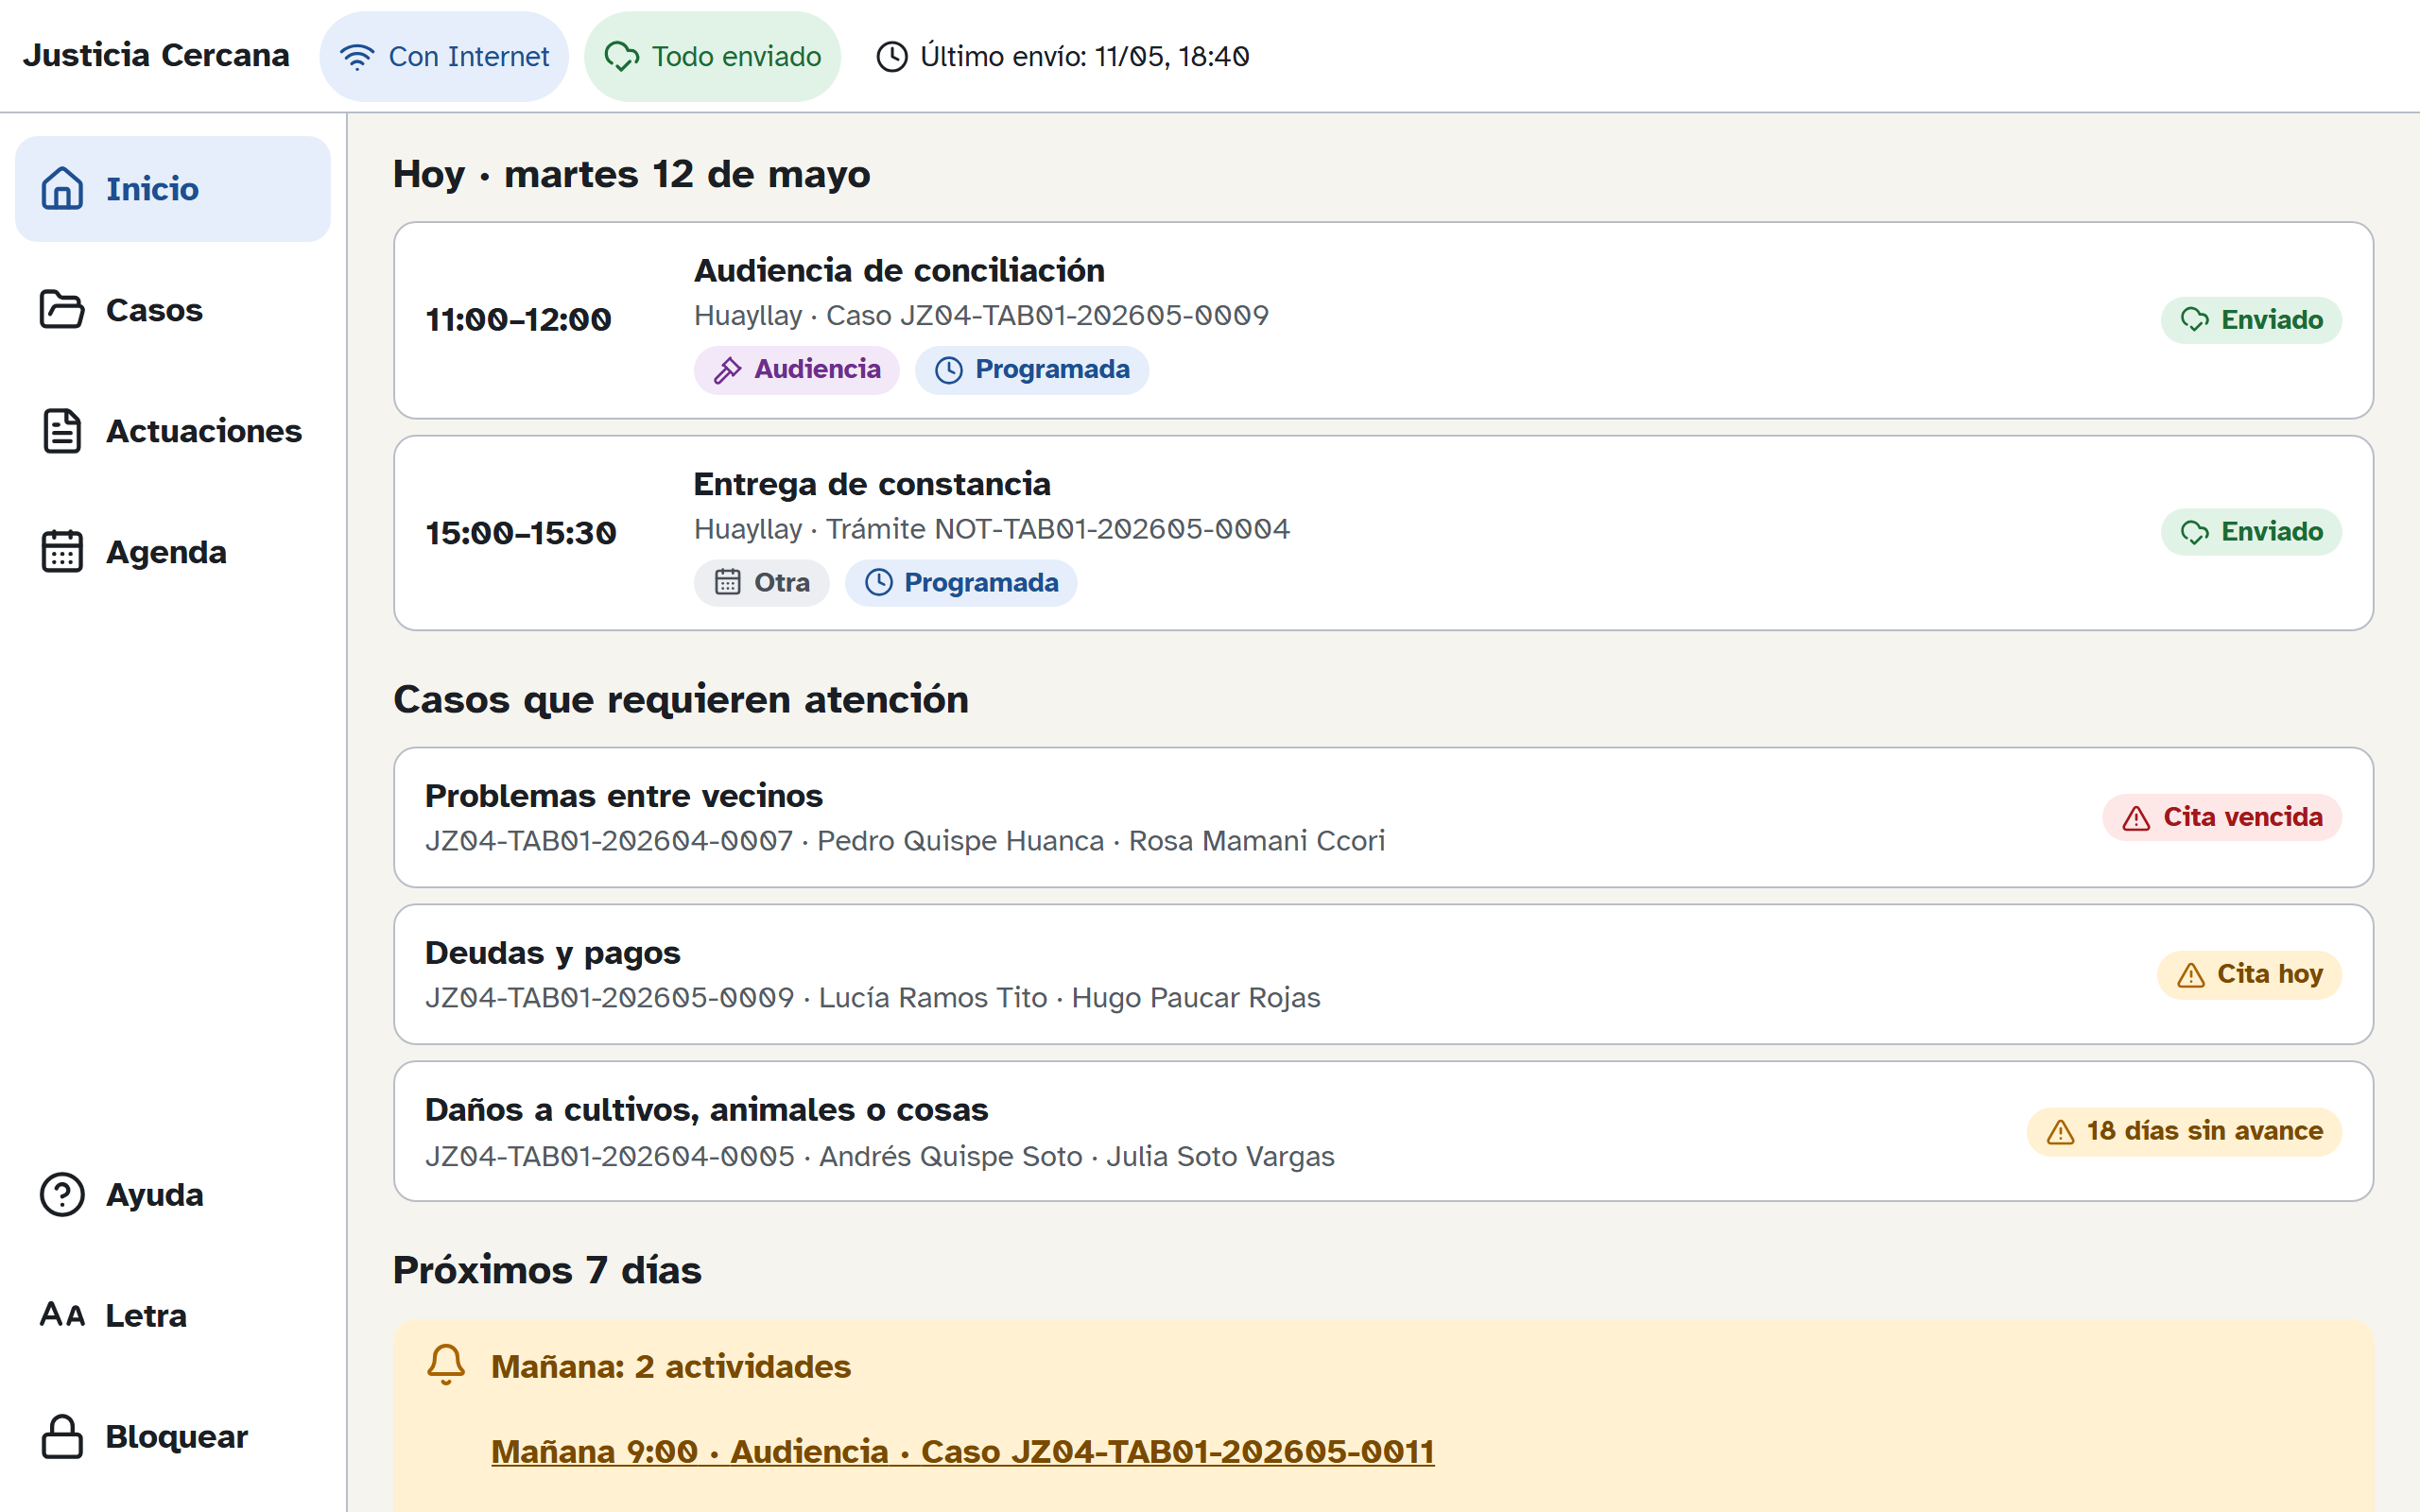
\includegraphics[width=\linewidth]{../../captures/P-01_inicio.png}\\[-2pt]{\footnotesize\raggedright\textbf{P-01.} Inicio: Hoy, casos que requieren atención con motivo en texto, próximos 7 días y accesos grandes \emph{(Cobertura y funcionamiento de los módulos)}\par}\end{minipage}\par\vspace{8pt}\noindent
\begin{minipage}[t]{0.49\textwidth}\centering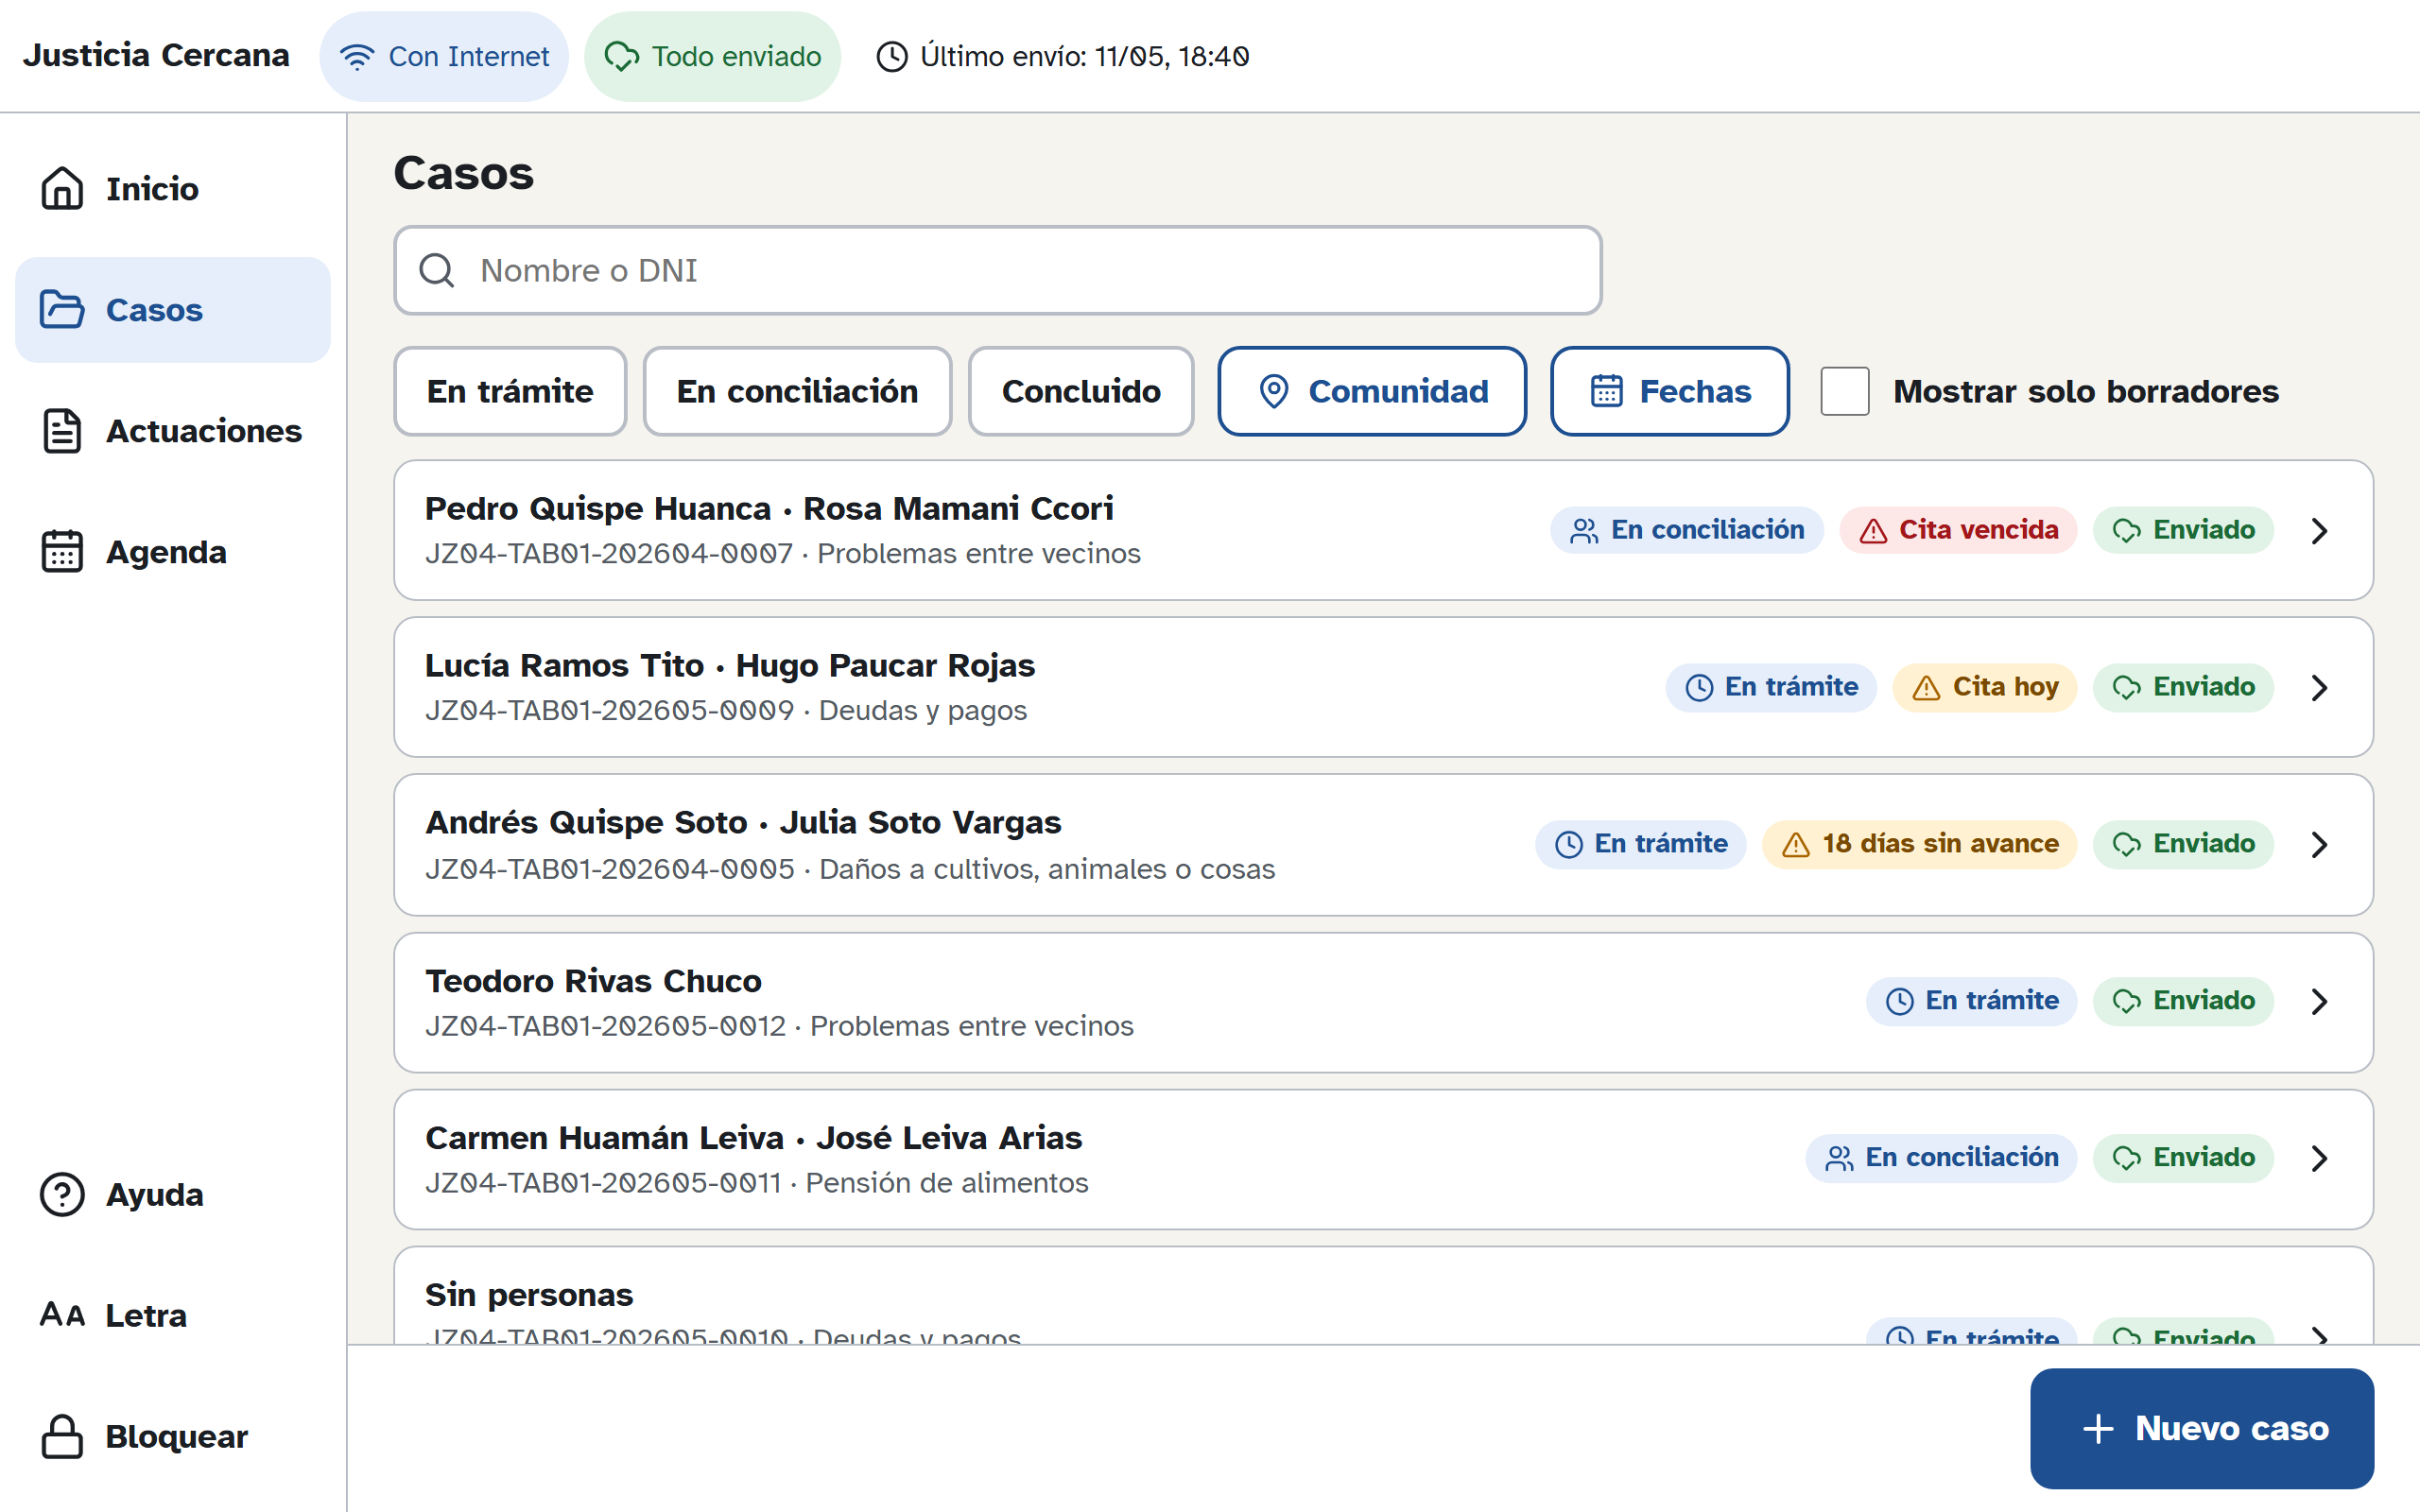
\includegraphics[width=\linewidth]{../../captures/P-02_casos-lista.png}\\[-2pt]{\footnotesize\raggedright\textbf{P-02.} Lista de casos: búsqueda, filtros como botones, motivo de atención, borrador y distintivo por registro \emph{(Cobertura y funcionamiento de los módulos)}\par}\end{minipage}\hfill
\begin{minipage}[t]{0.49\textwidth}\centering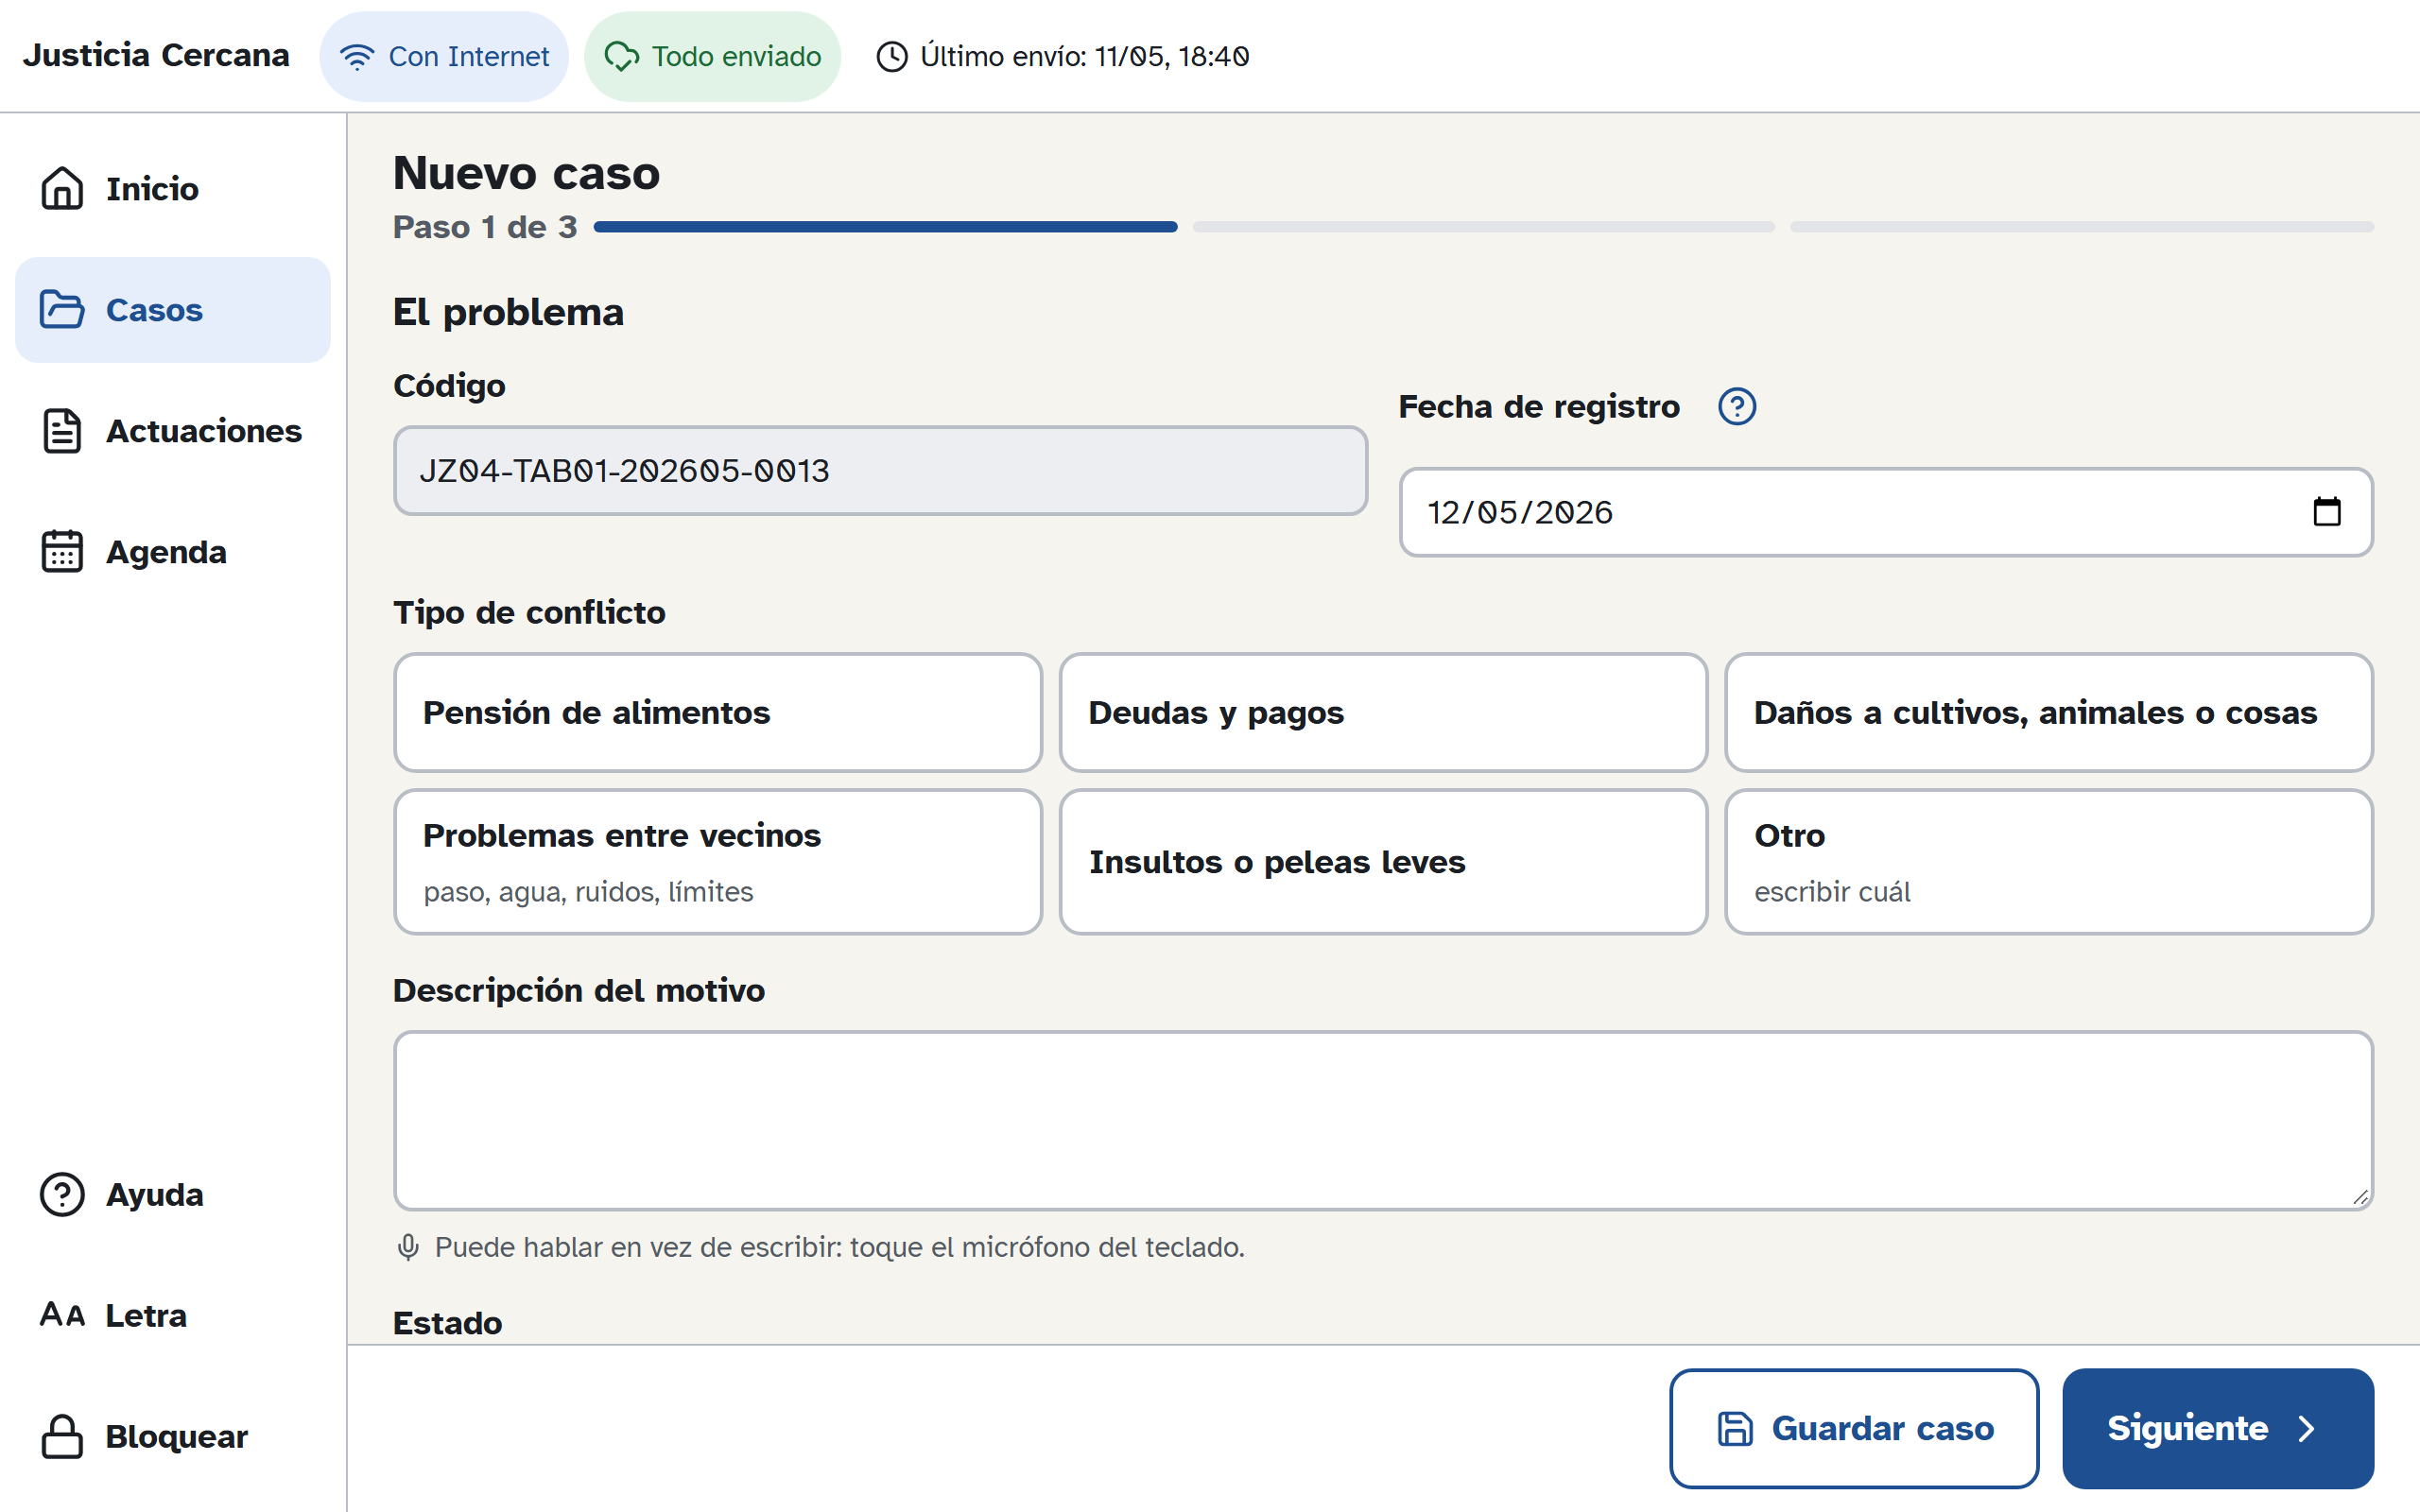
\includegraphics[width=\linewidth]{../../captures/P-03_caso-nuevo.png}\\[-2pt]{\footnotesize\raggedright\textbf{P-03.} Caso nuevo, paso 1 de 3: código generado sin conexión, tipos con botones grandes \emph{(Cobertura y funcionamiento de los módulos)}\par}\end{minipage}\par\vspace{8pt}\noindent
\begin{minipage}[t]{0.49\textwidth}\centering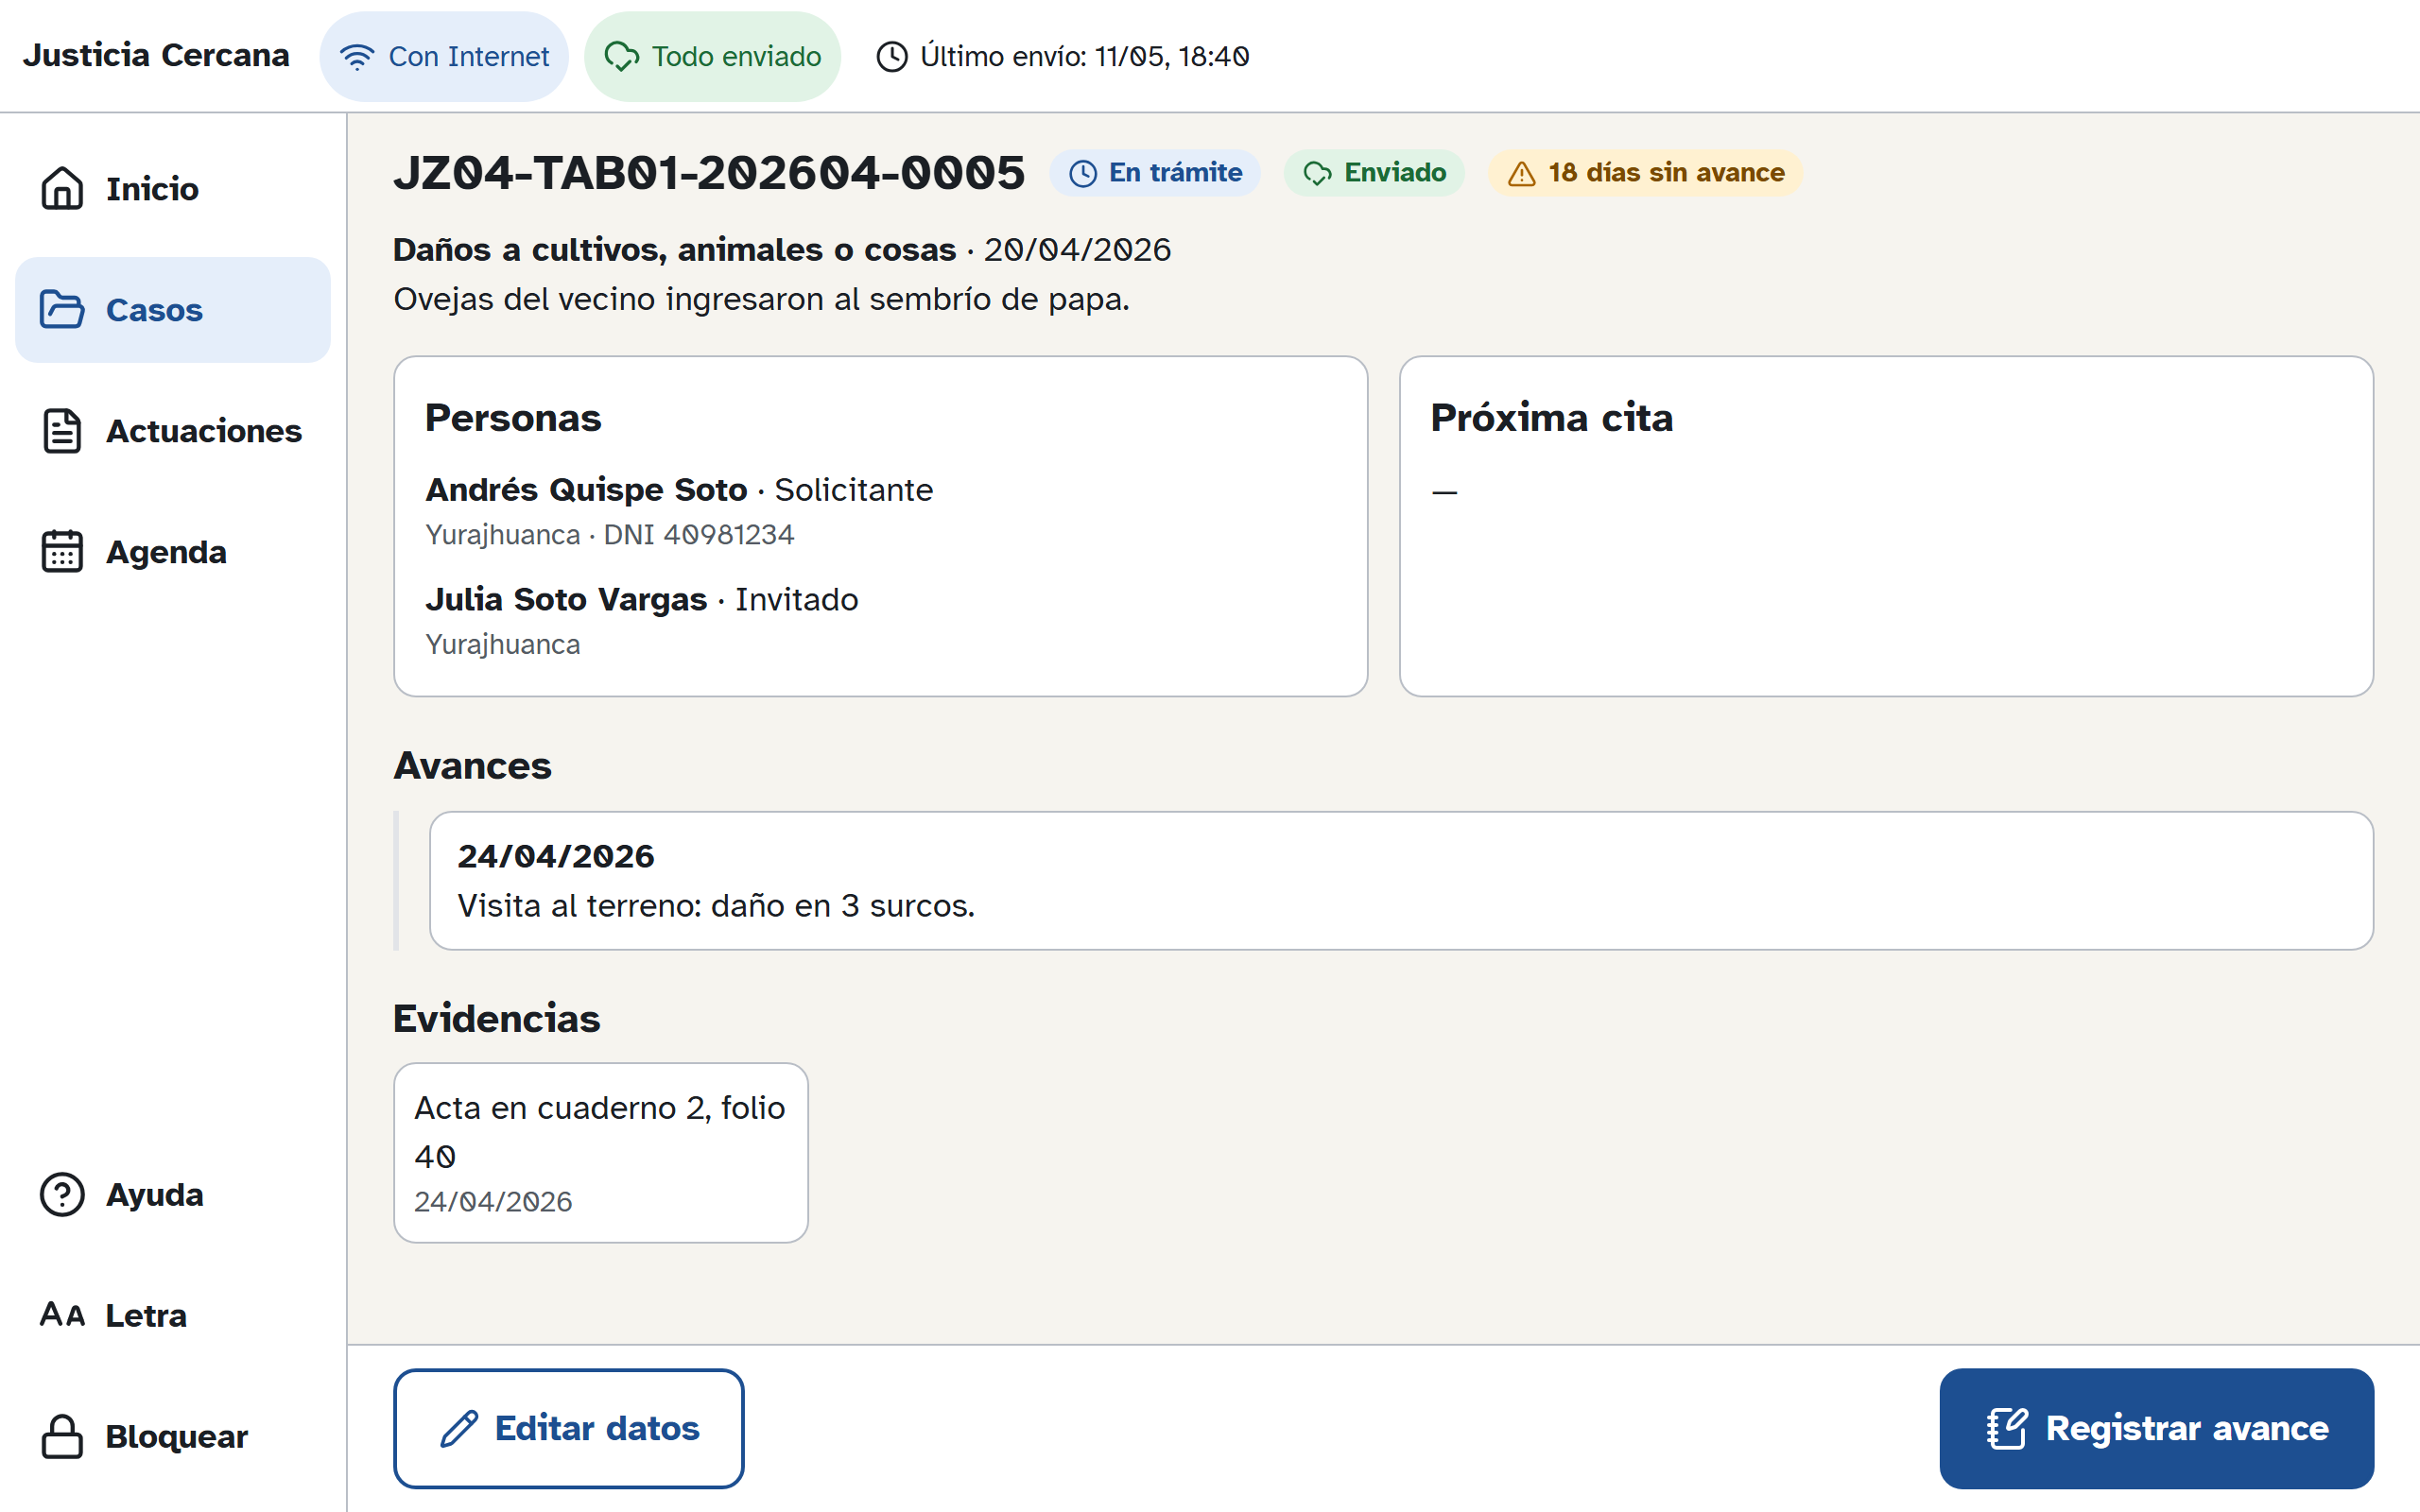
\includegraphics[width=\linewidth]{../../captures/P-04_caso-detalle.png}\\[-2pt]{\footnotesize\raggedright\textbf{P-04.} Detalle: estado, distintivo, motivo ``15+ días sin avance'', historial, evidencias; [Registrar avance] abajo a la derecha \emph{(Cobertura y funcionamiento de los módulos)}\par}\end{minipage}\hfill
\begin{minipage}[t]{0.49\textwidth}\centering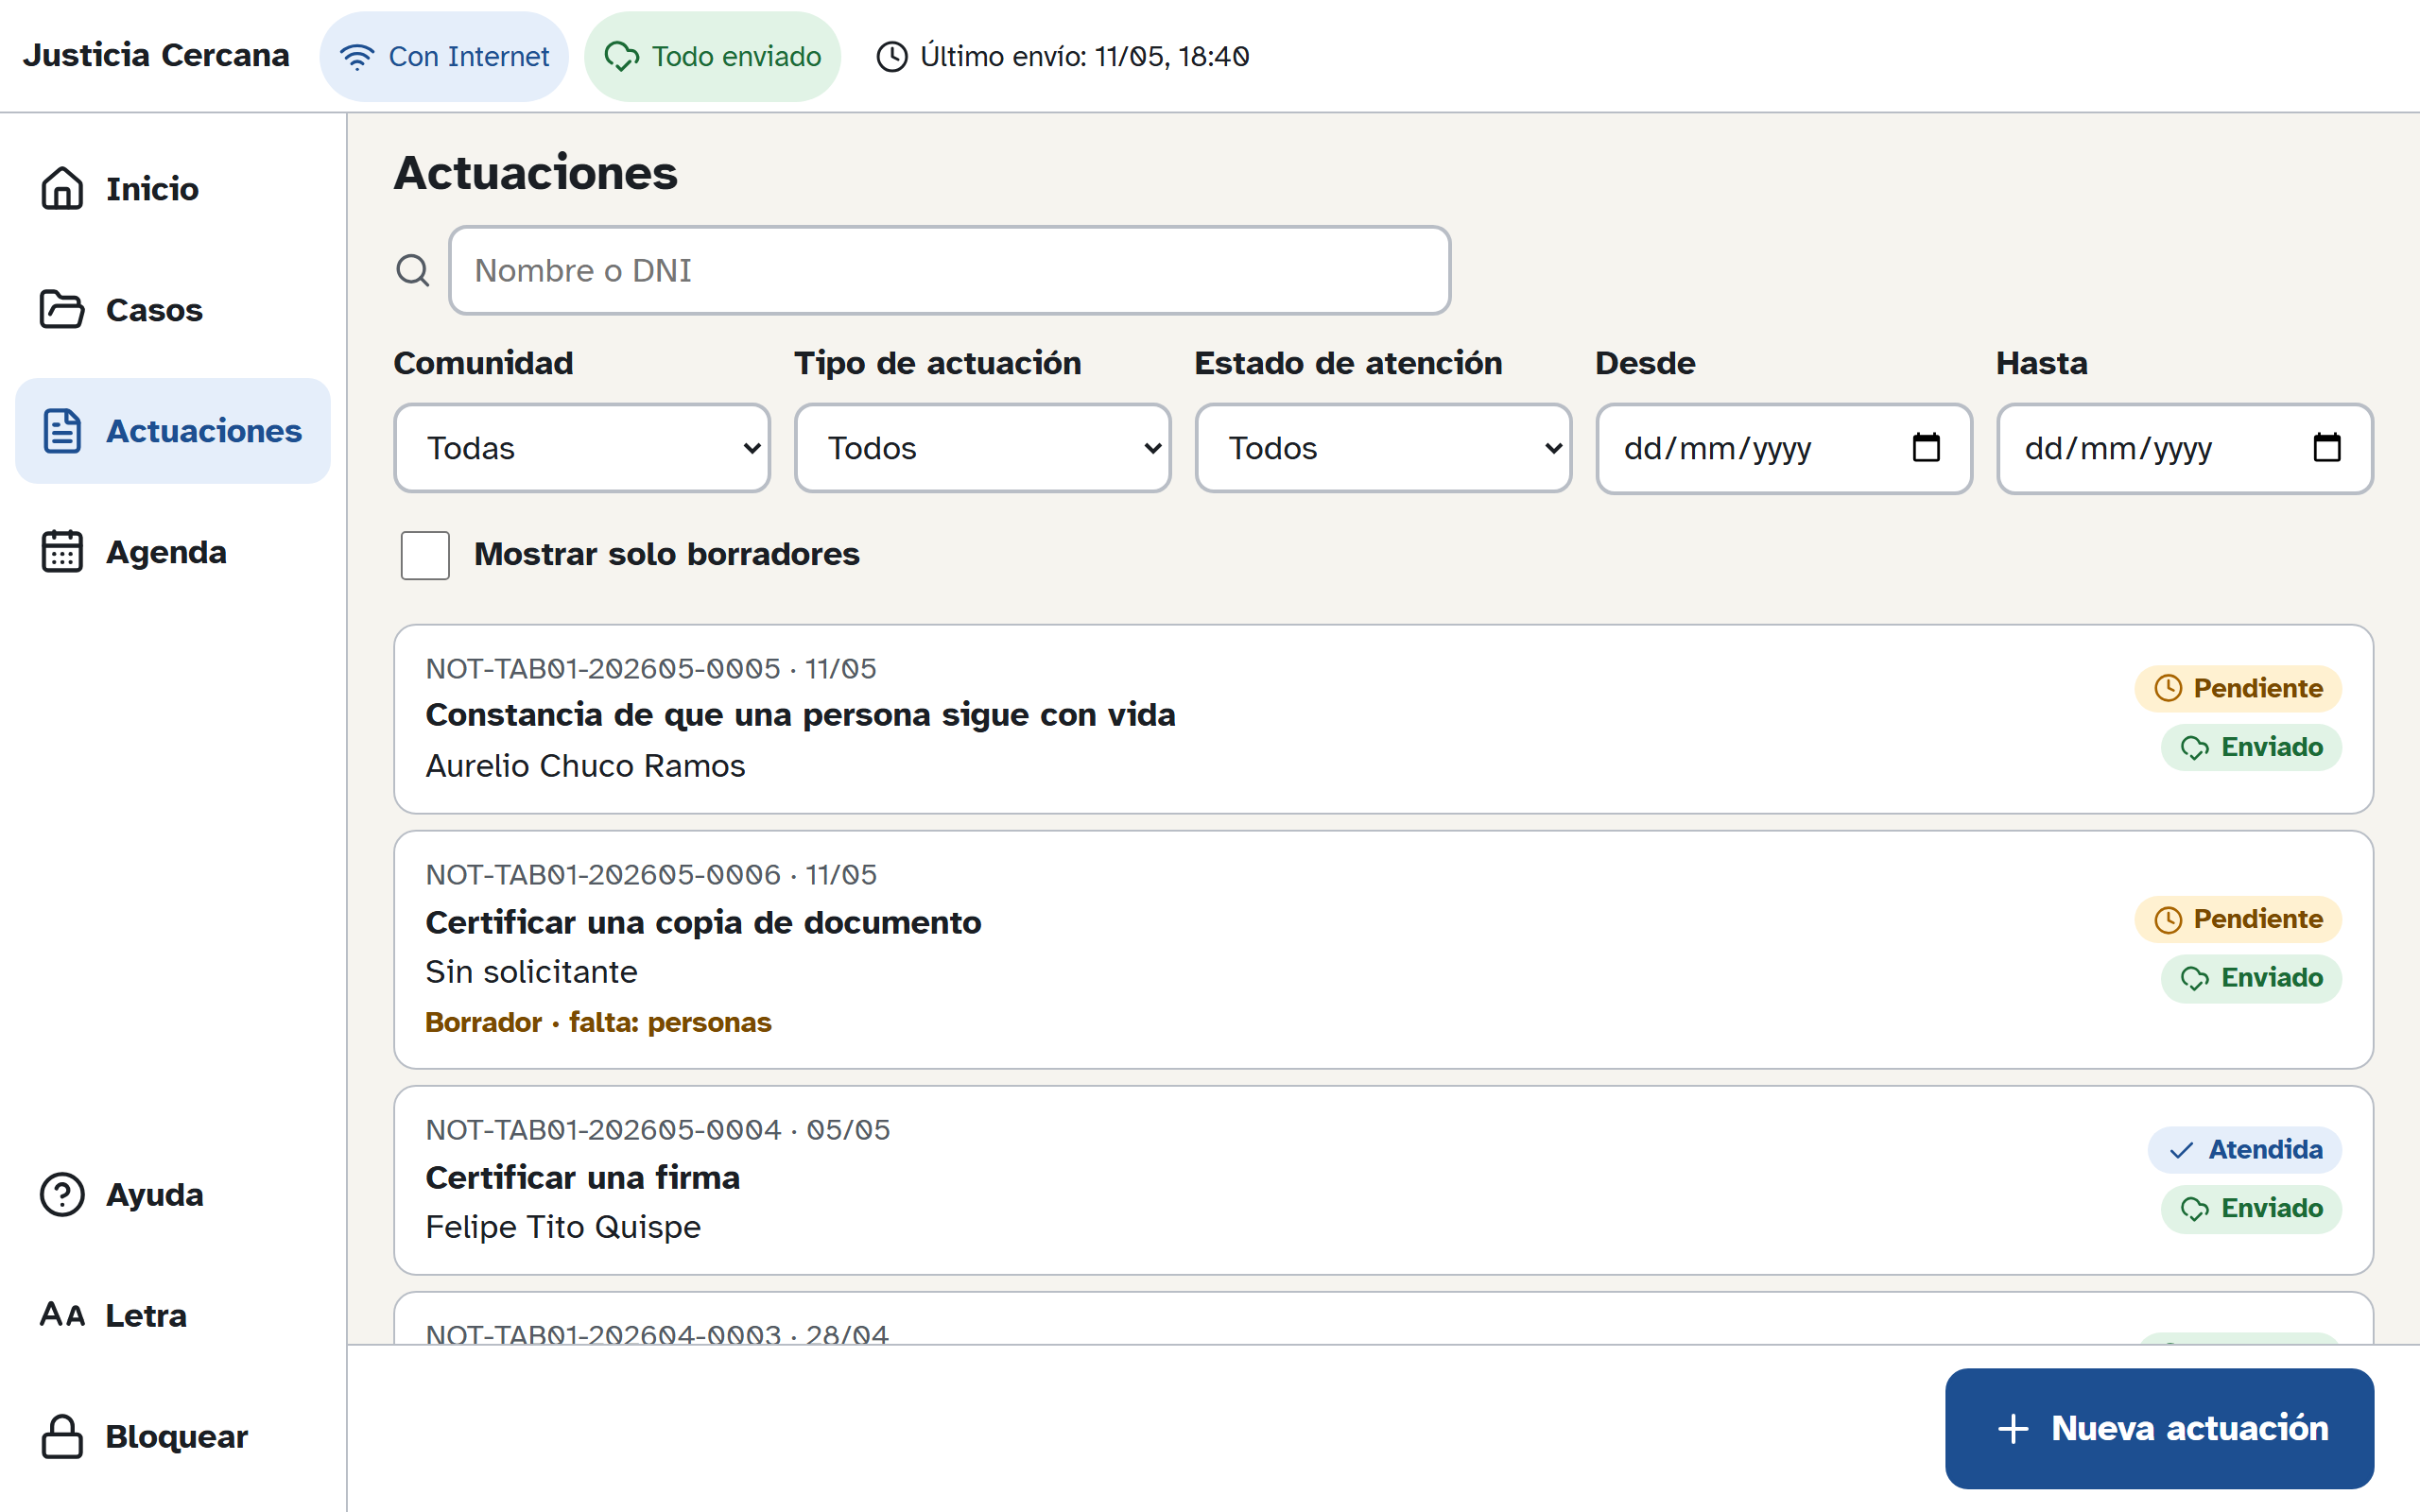
\includegraphics[width=\linewidth]{../../captures/P-05_actuaciones-lista.png}\\[-2pt]{\footnotesize\raggedright\textbf{P-05.} Lista de actuaciones con estado de atención, borrador y distintivo \emph{(Cobertura y funcionamiento de los módulos)}\par}\end{minipage}\par\vspace{8pt}\noindent
\begin{minipage}[t]{0.49\textwidth}\centering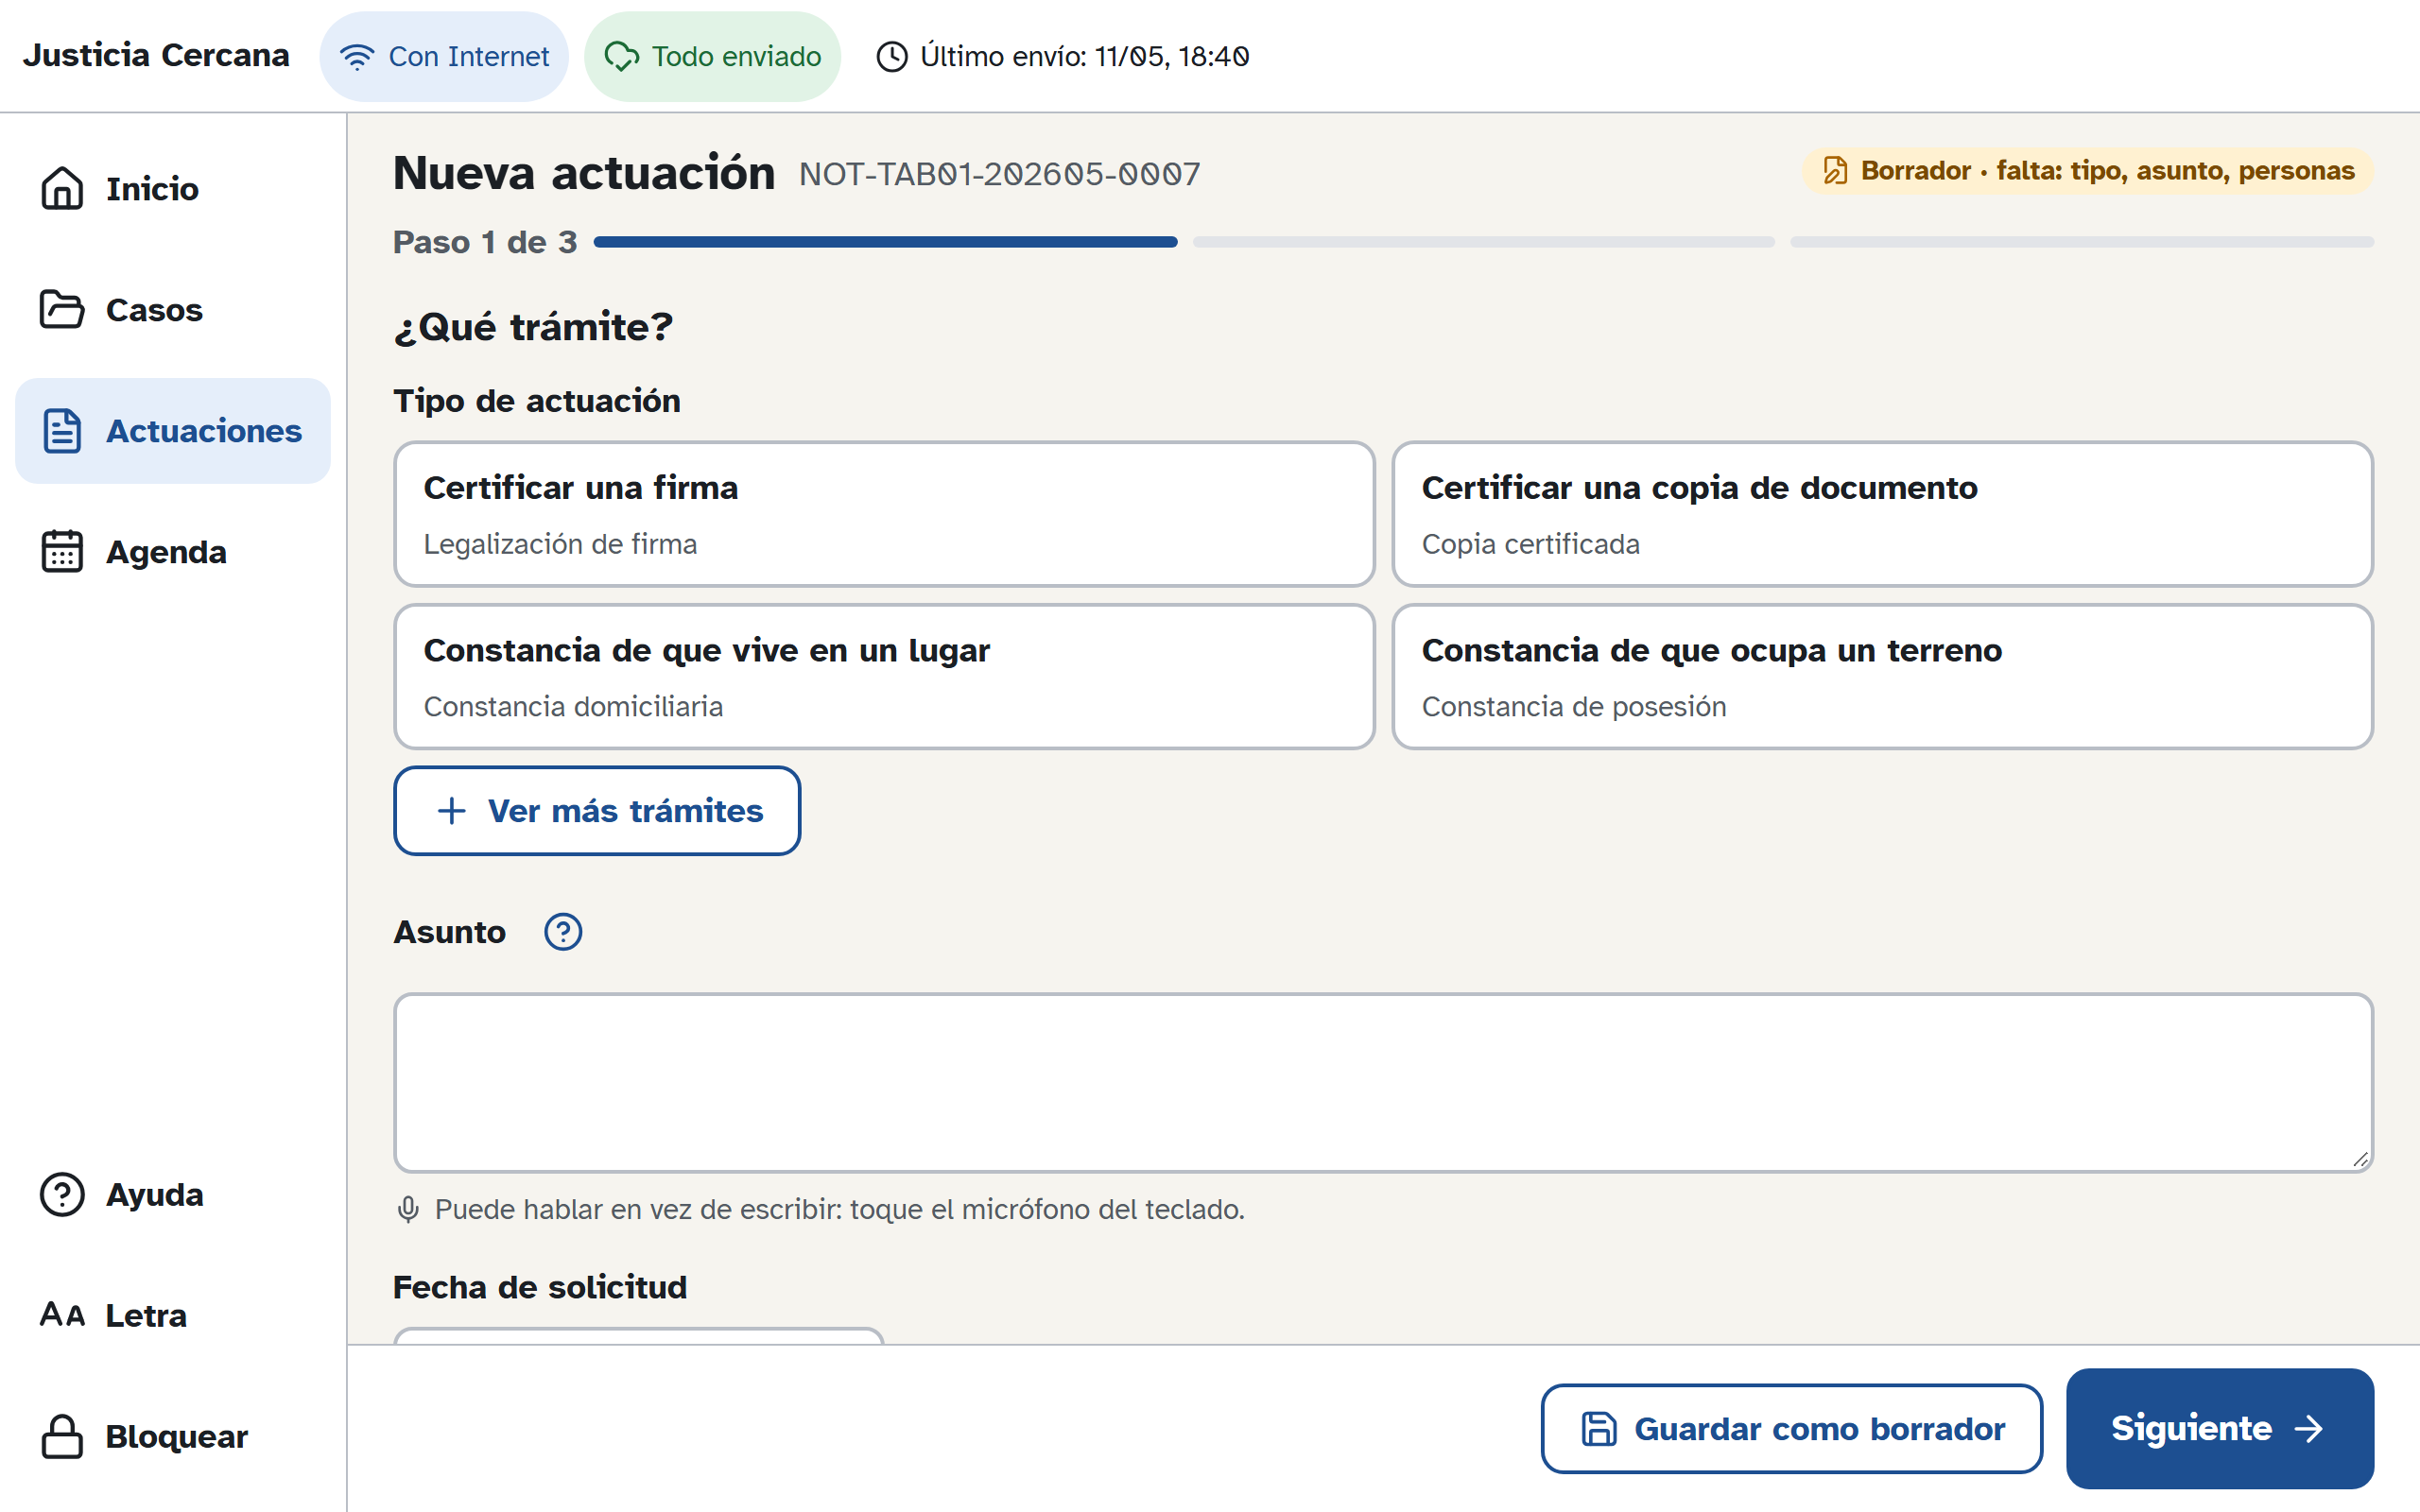
\includegraphics[width=\linewidth]{../../captures/P-06_actuacion-nueva.png}\\[-2pt]{\footnotesize\raggedright\textbf{P-06.} Actuación nueva, paso 1: 4 tarjetas en lenguaje cotidiano + [Ver más trámites] \emph{(Cobertura y funcionamiento de los módulos)}\par}\end{minipage}\hfill
\begin{minipage}[t]{0.49\textwidth}\centering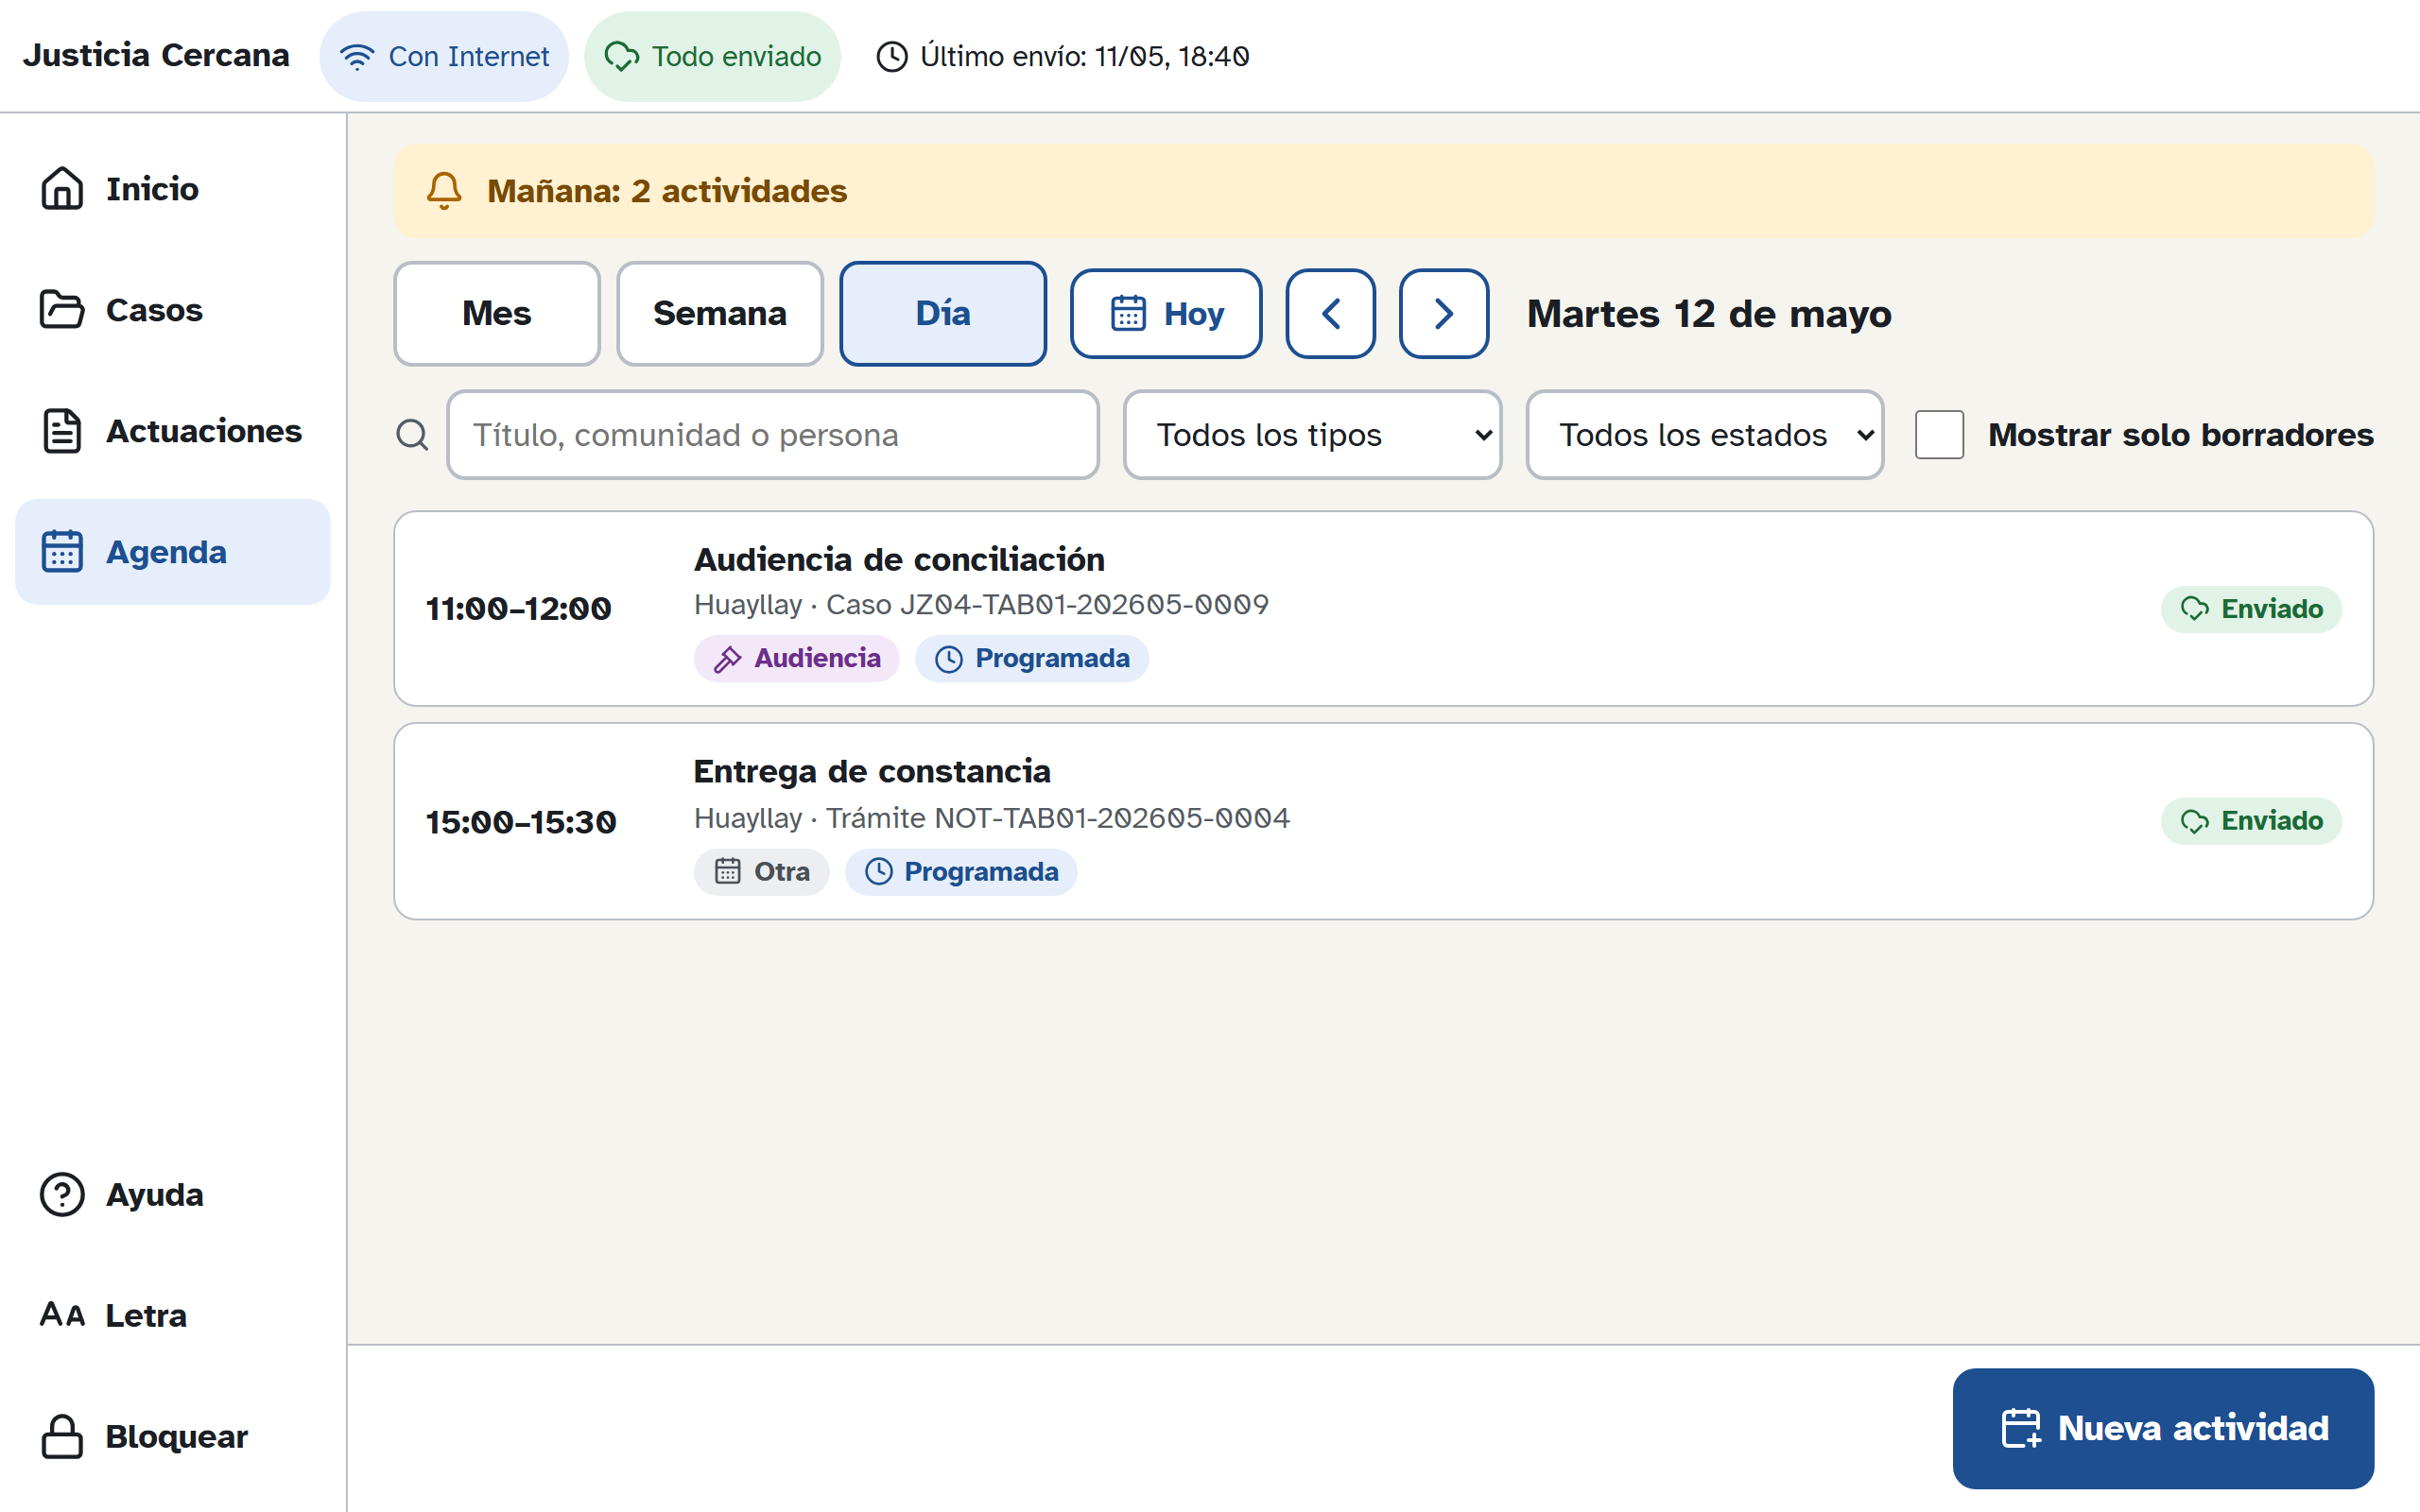
\includegraphics[width=\linewidth]{../../captures/P-07_agenda-dia.png}\\[-2pt]{\footnotesize\raggedright\textbf{P-07.} Agenda Día (hoy) \emph{(Cobertura y funcionamiento de los módulos)}\par}\end{minipage}\par\vspace{8pt}\noindent
\begin{minipage}[t]{0.49\textwidth}\centering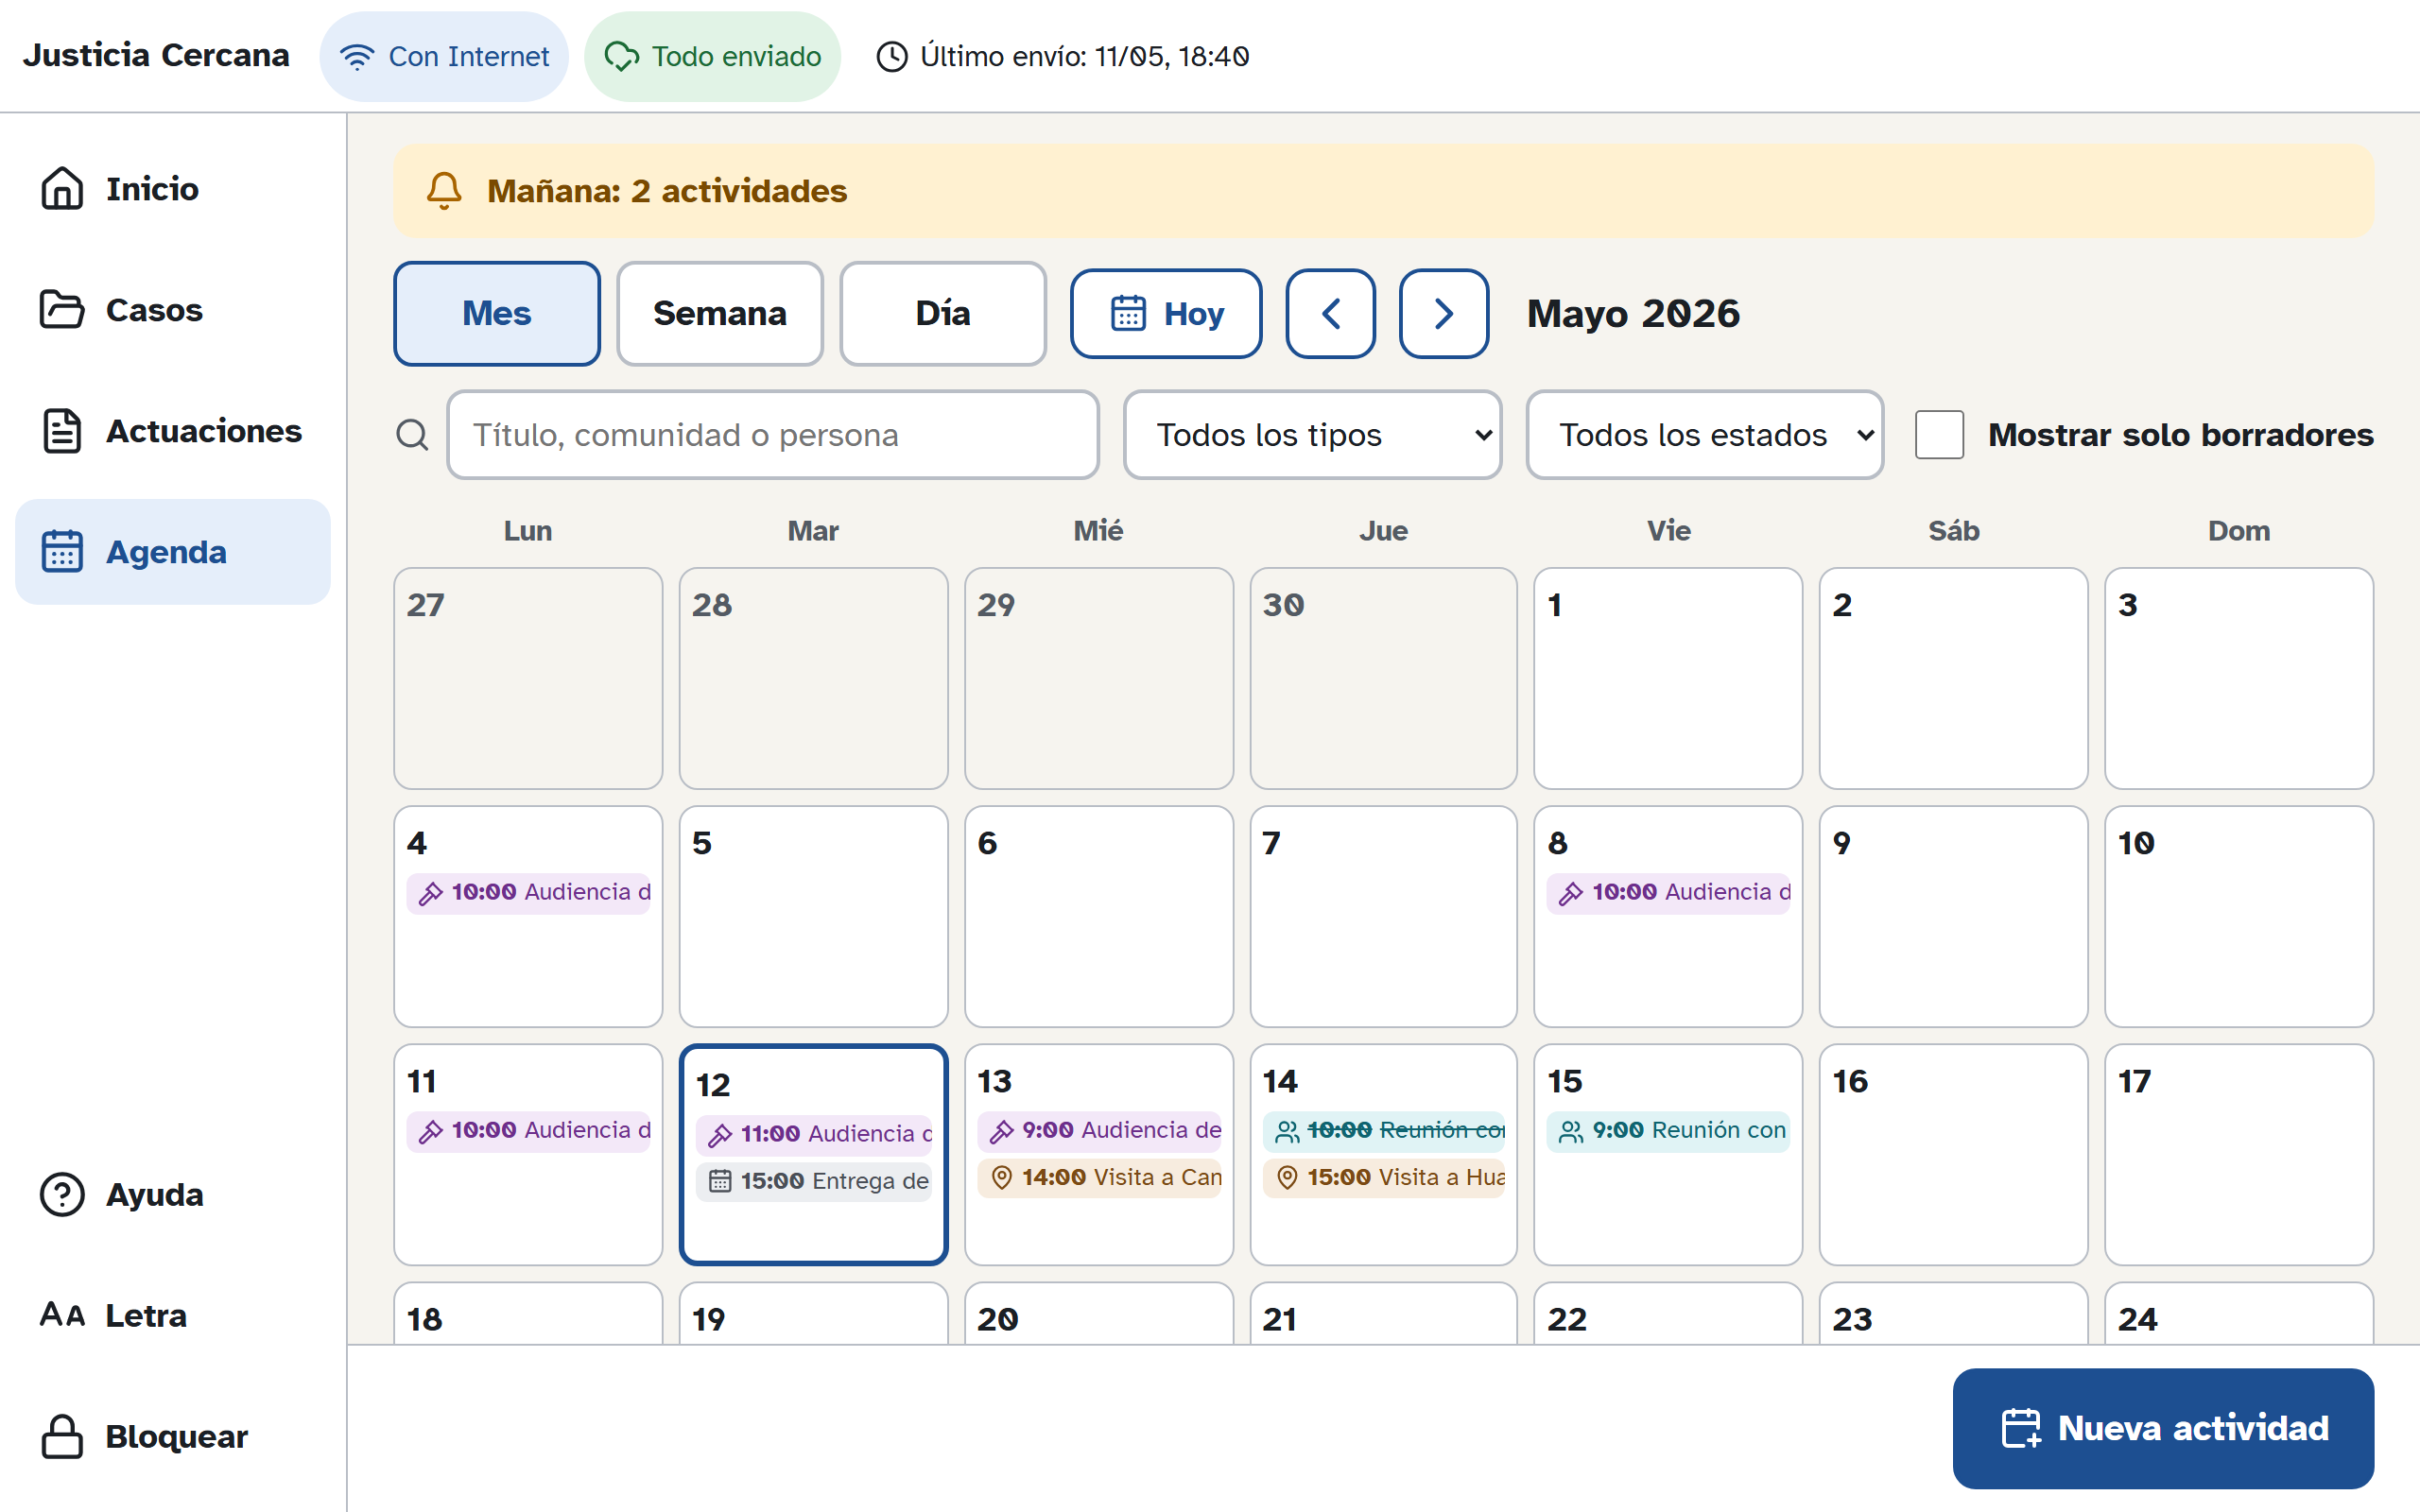
\includegraphics[width=\linewidth]{../../captures/P-07_agenda-mes.png}\\[-2pt]{\footnotesize\raggedright\textbf{P-07.} Agenda Mes: hasta 3 actividades por día y ``+2 más'' \emph{(Cobertura y funcionamiento de los módulos)}\par}\end{minipage}\hfill
\begin{minipage}[t]{0.49\textwidth}\centering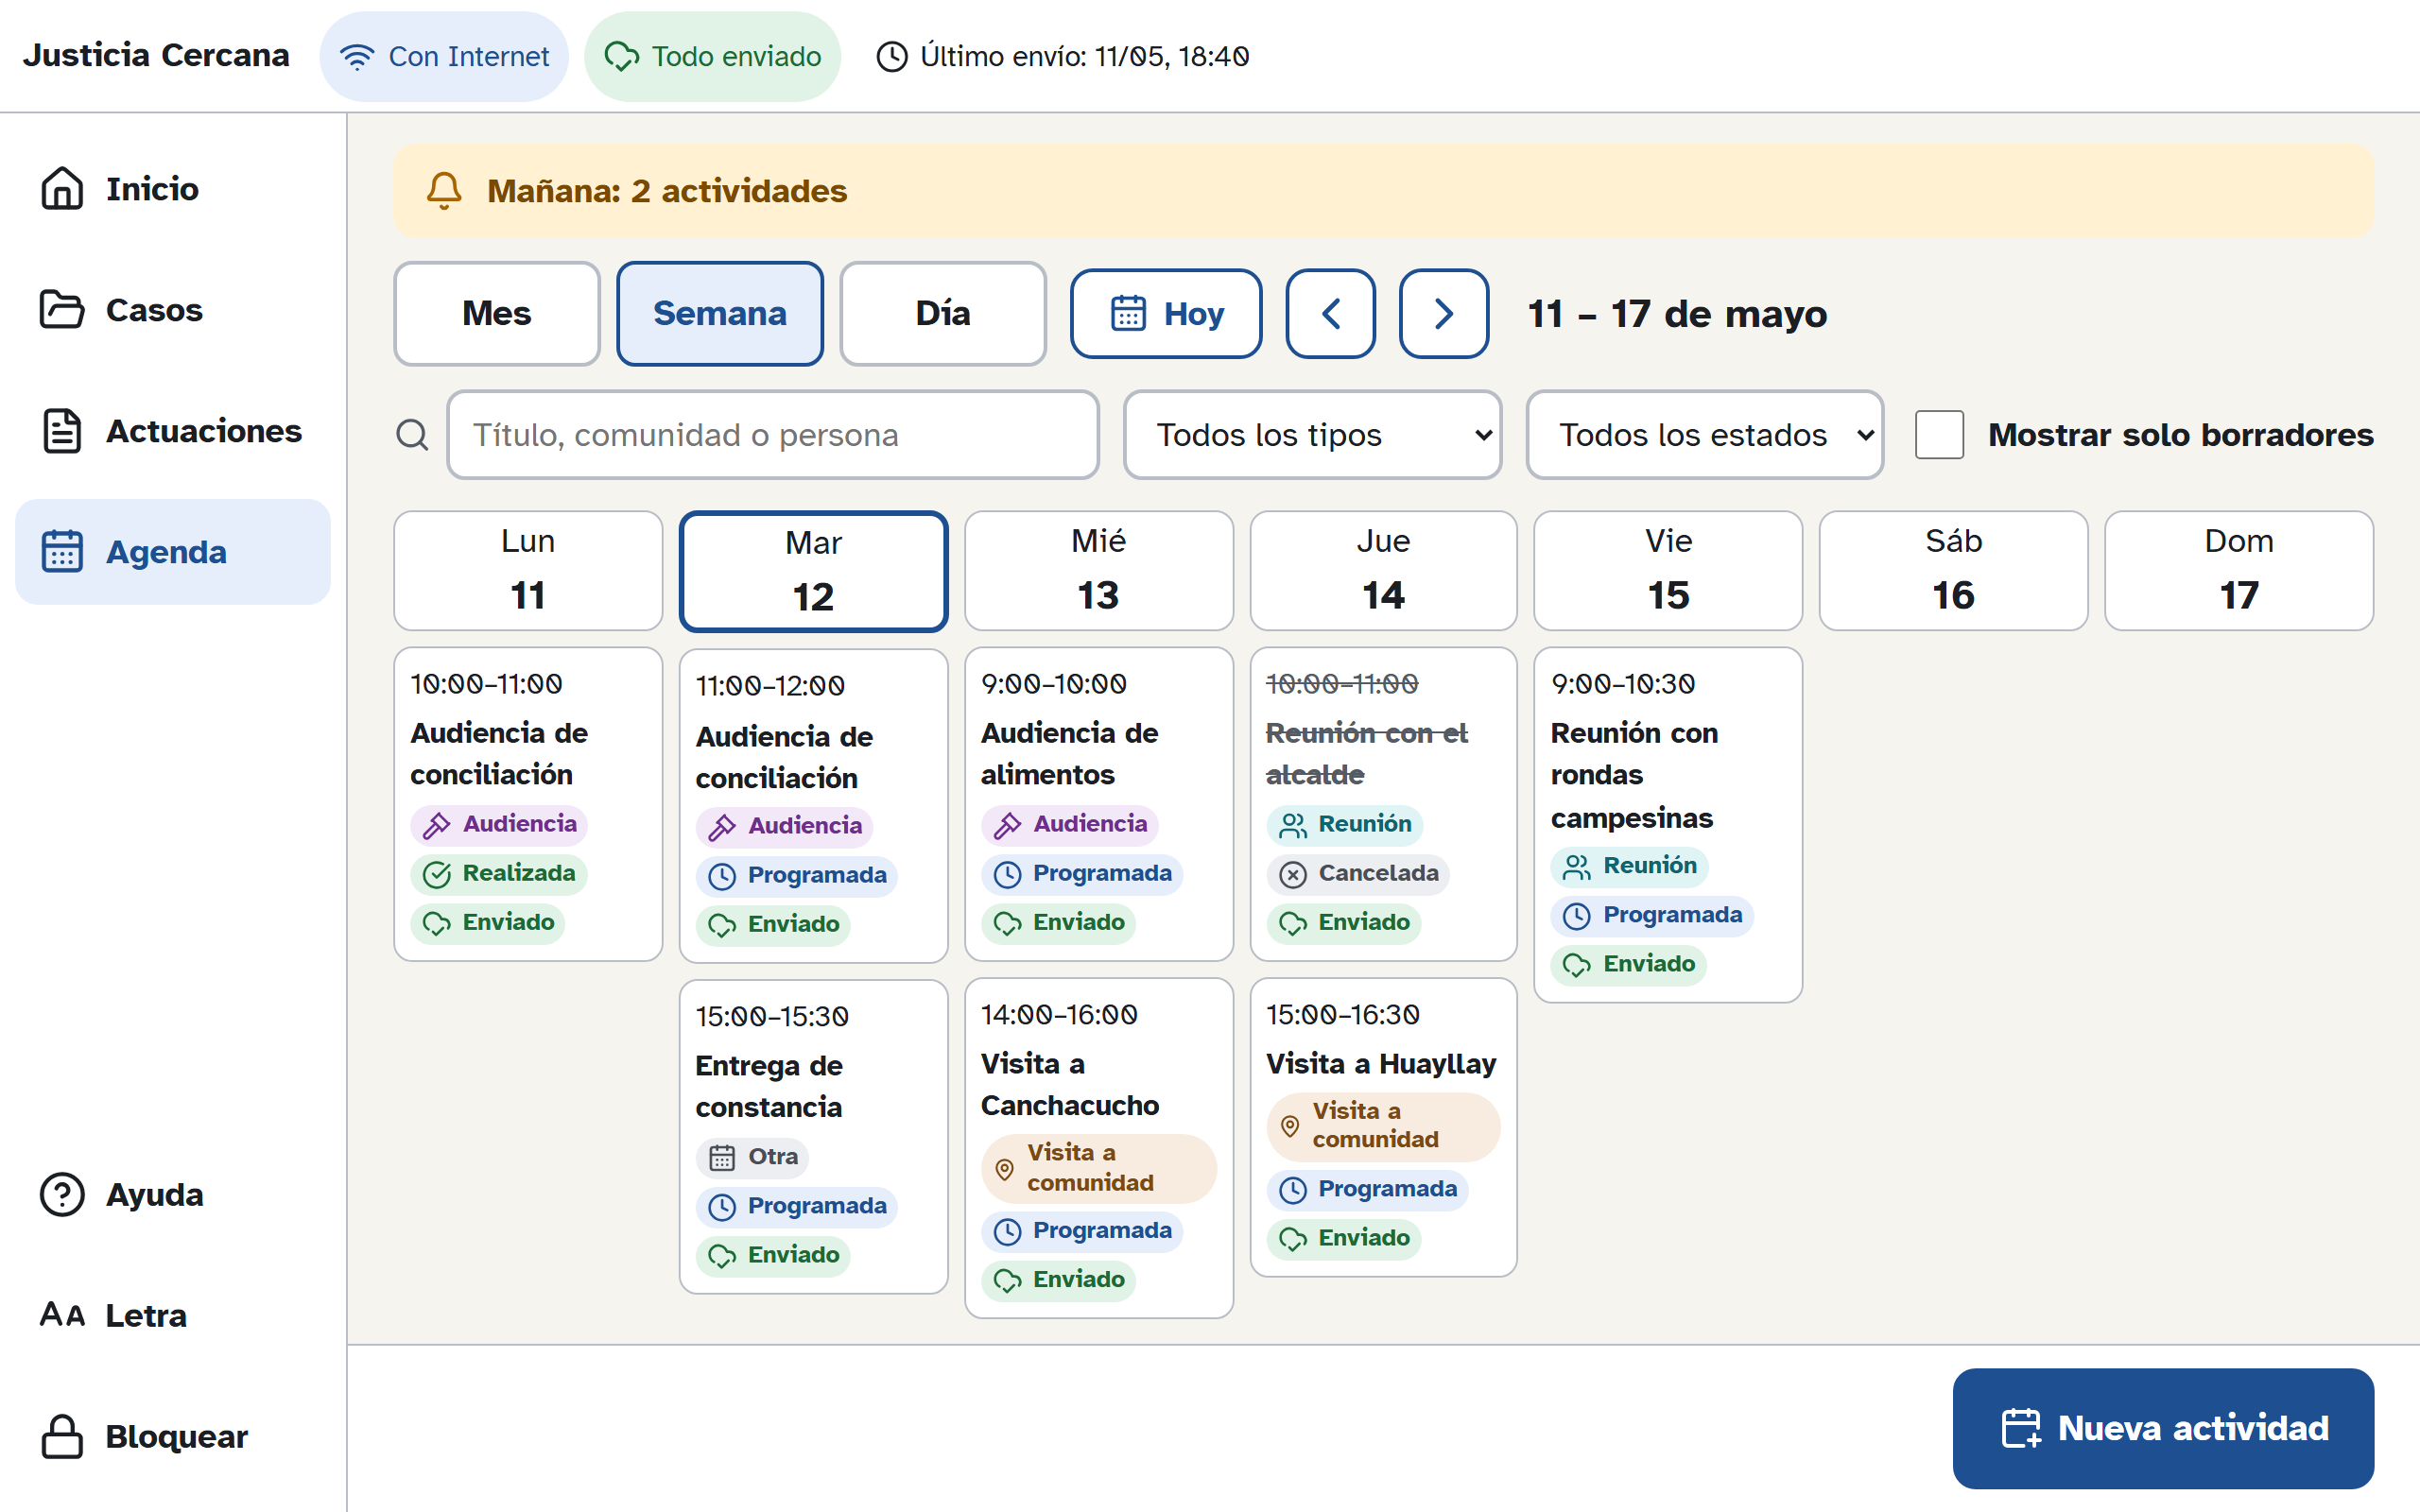
\includegraphics[width=\linewidth]{../../captures/P-07_agenda-semana.png}\\[-2pt]{\footnotesize\raggedright\textbf{P-07.} Agenda Semana: franja ``Mañana: 2 actividades'', categorías color + ícono + texto, estados \emph{(Cobertura y funcionamiento de los módulos)}\par}\end{minipage}\par\vspace{8pt}\noindent
\begin{minipage}[t]{0.49\textwidth}\centering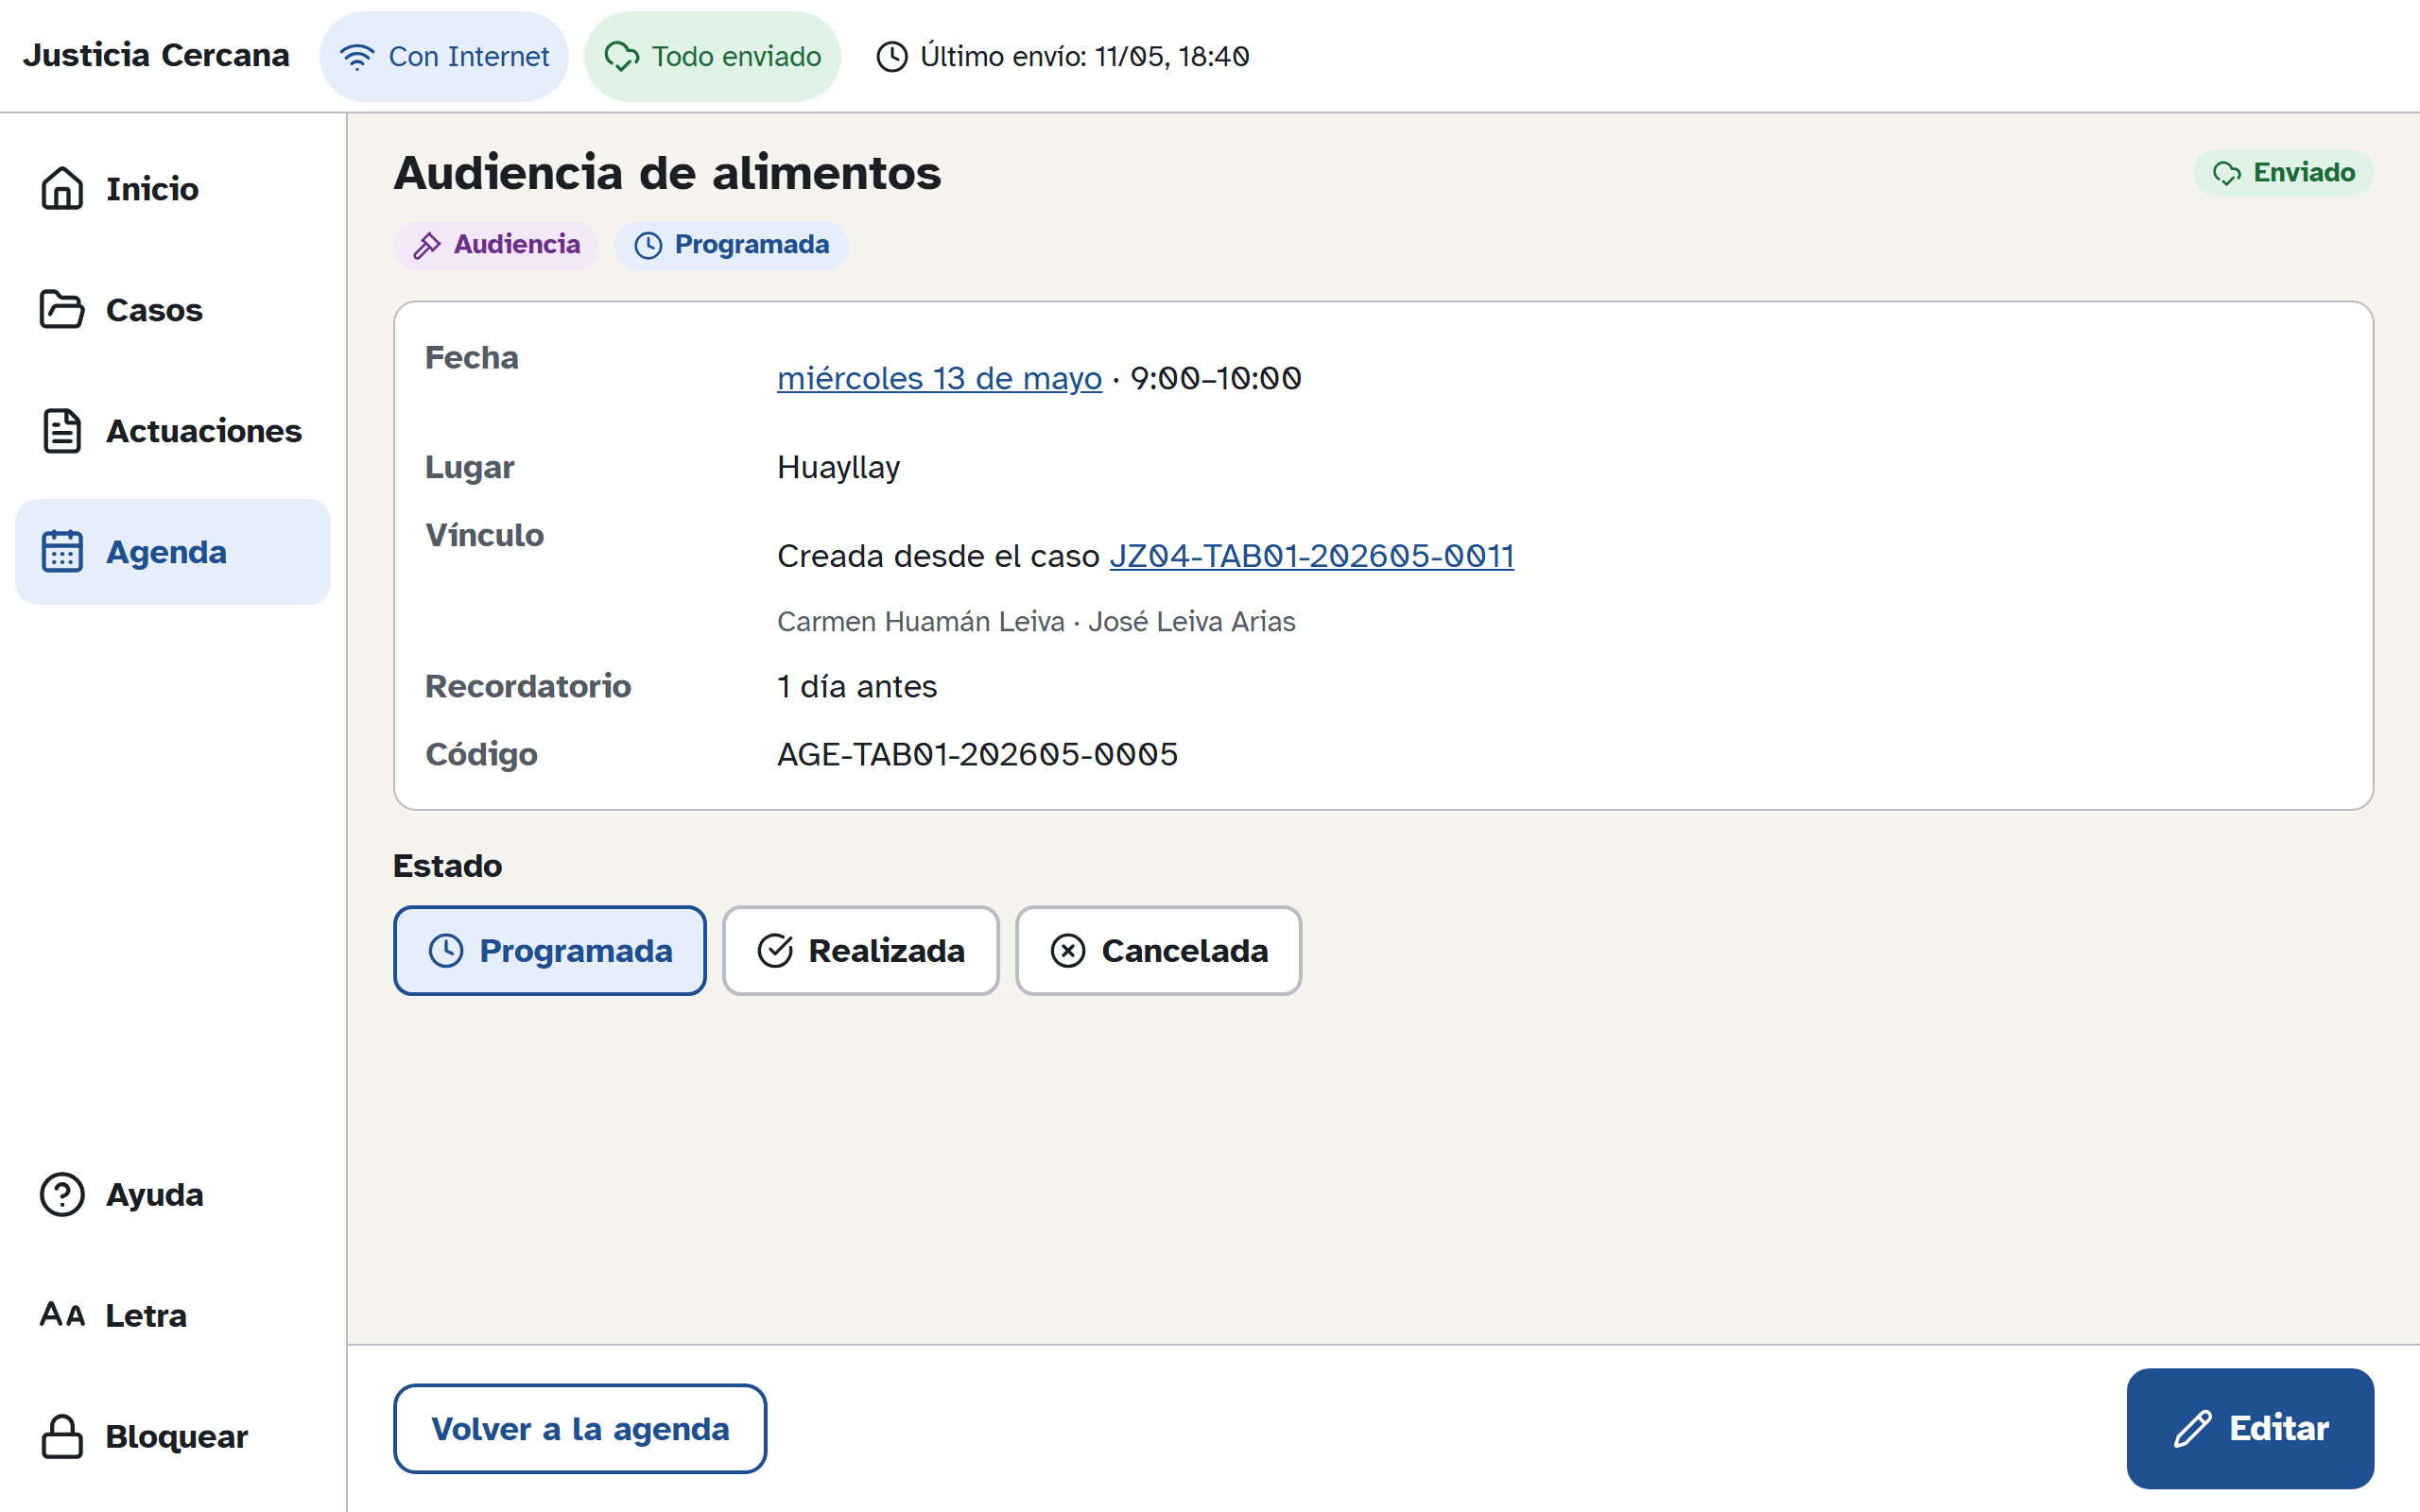
\includegraphics[width=\linewidth]{../../captures/P-08_actividad-detalle.png}\\[-2pt]{\footnotesize\raggedright\textbf{P-08.} Detalle de actividad: ``Creada desde el caso'' con enlace \emph{(Cobertura y funcionamiento de los módulos)}\par}\end{minipage}\hfill
\begin{minipage}[t]{0.49\textwidth}\centering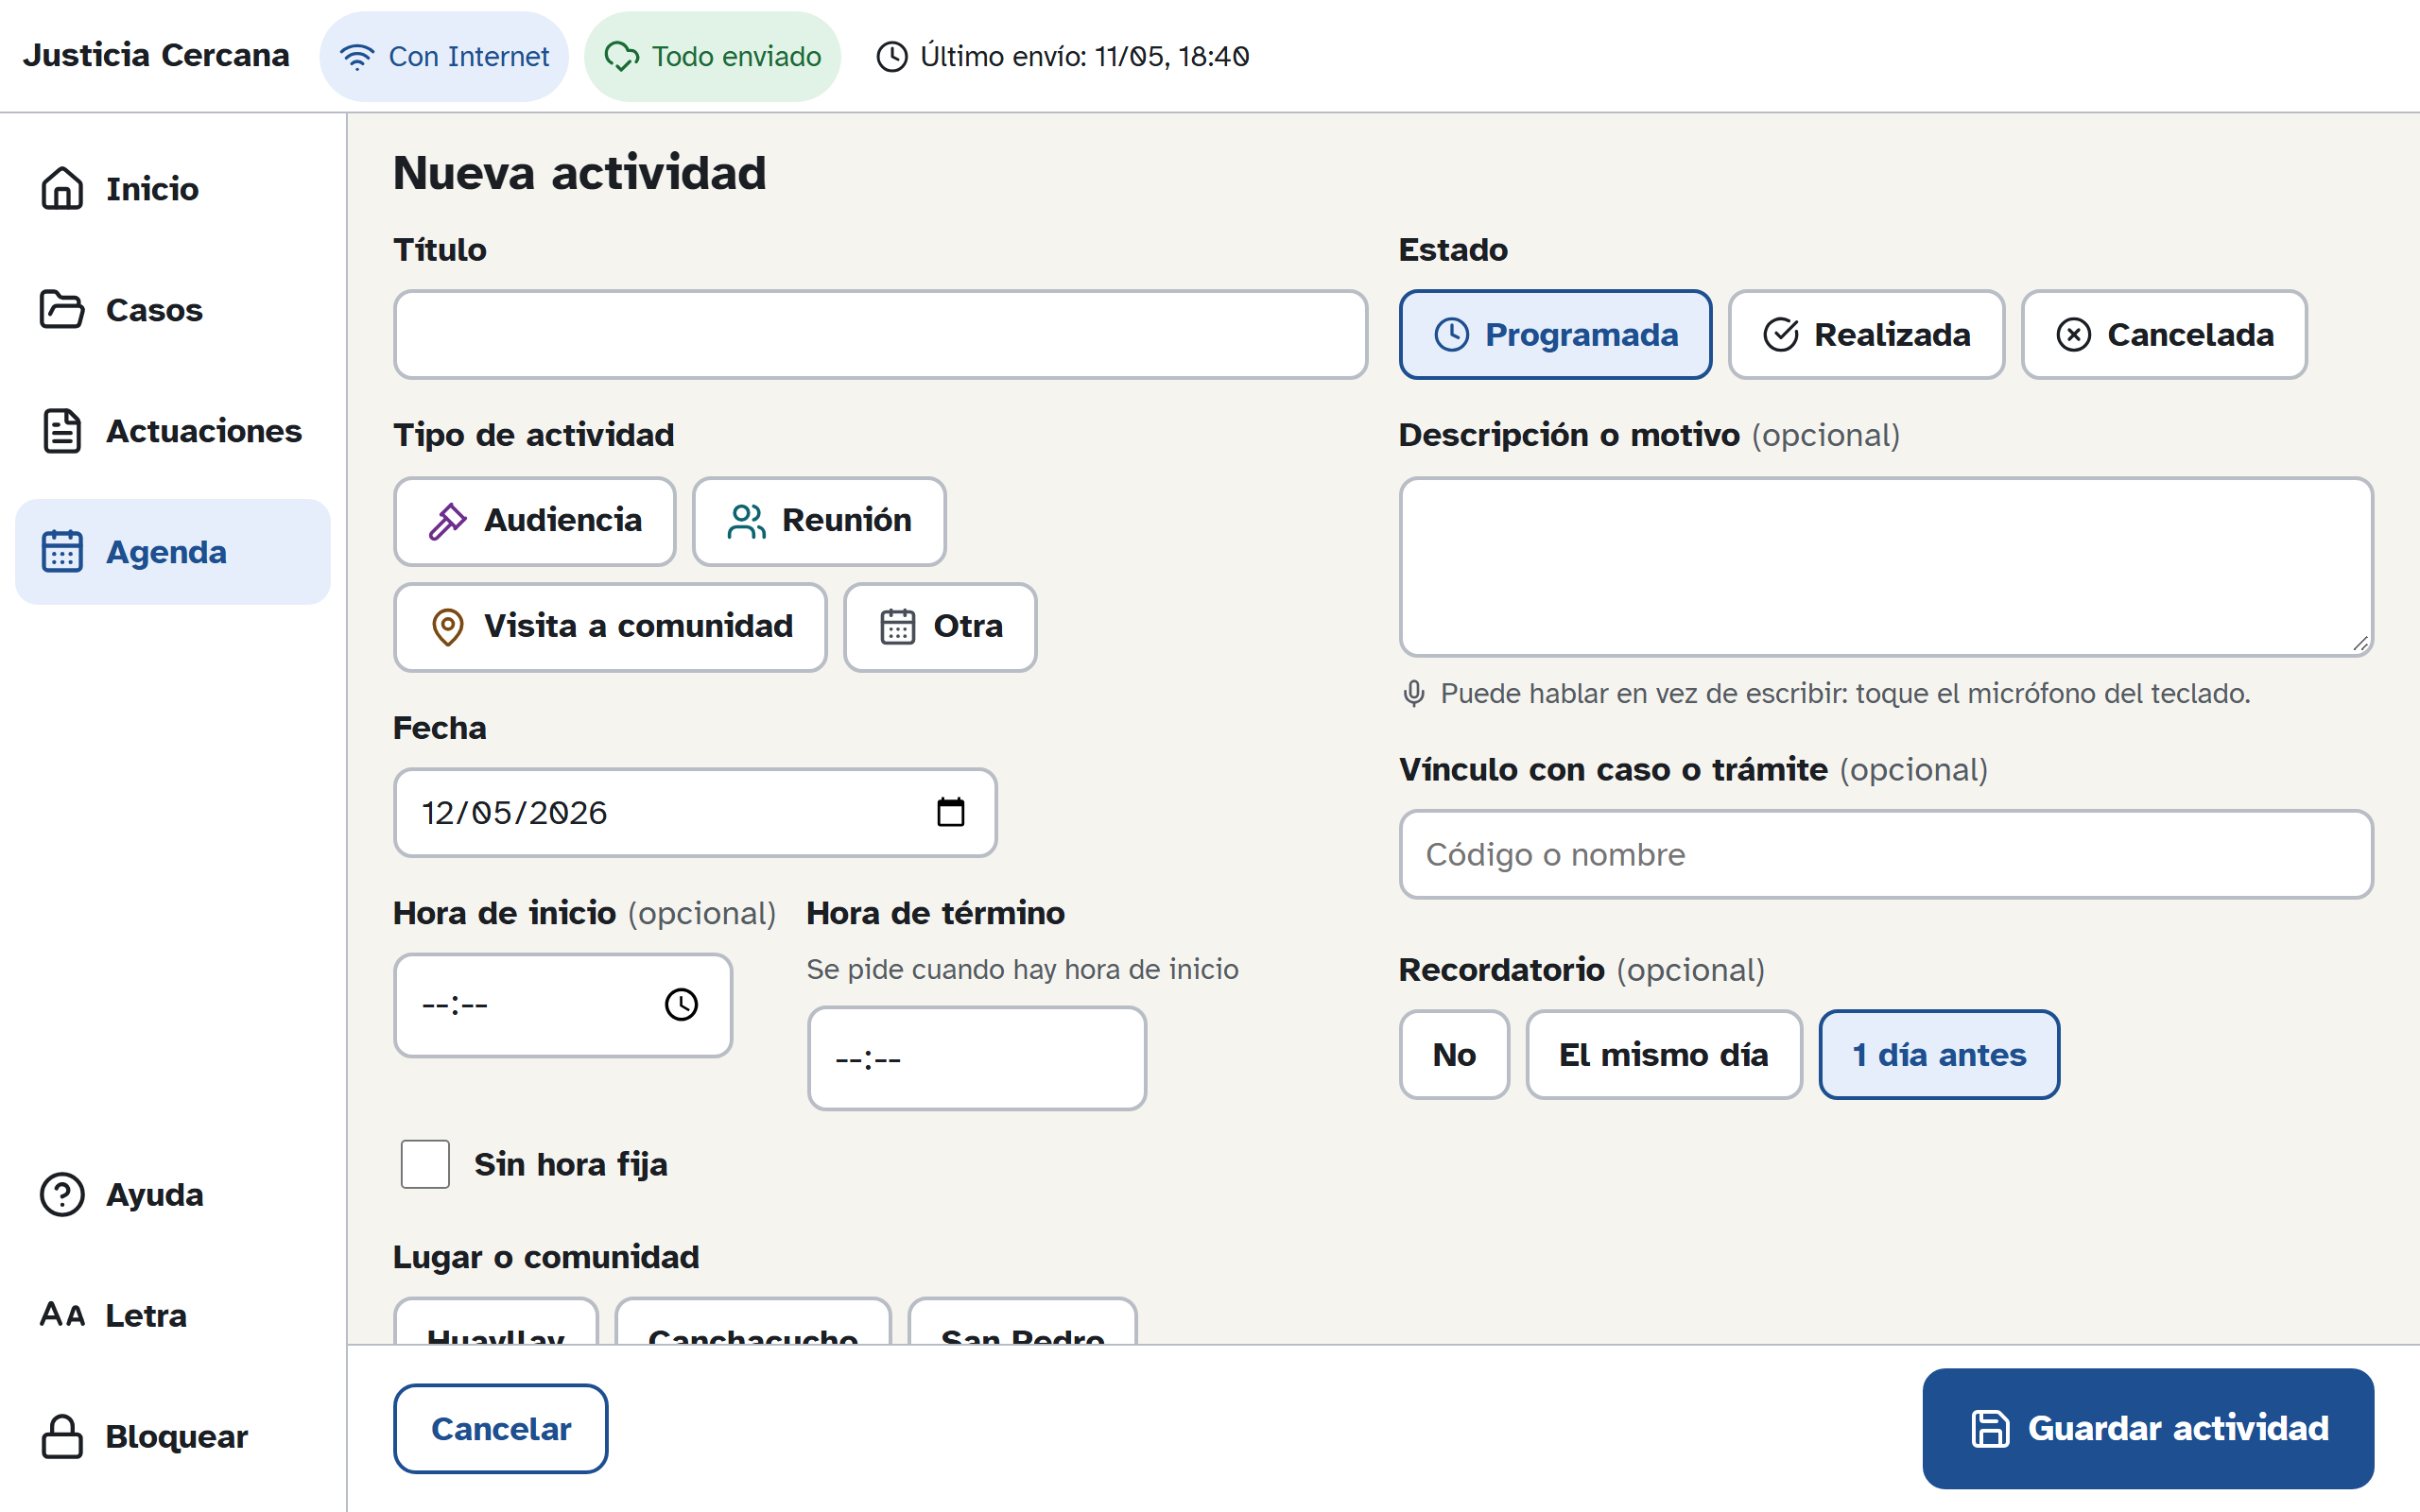
\includegraphics[width=\linewidth]{../../captures/P-08_actividad-nueva.png}\\[-2pt]{\footnotesize\raggedright\textbf{P-08.} Actividad nueva: todos los campos, ``(opcional)'', condicional de hora de término \emph{(Cobertura y funcionamiento de los módulos)}\par}\end{minipage}\par\vspace{8pt}\noindent
\begin{minipage}[t]{0.49\textwidth}\centering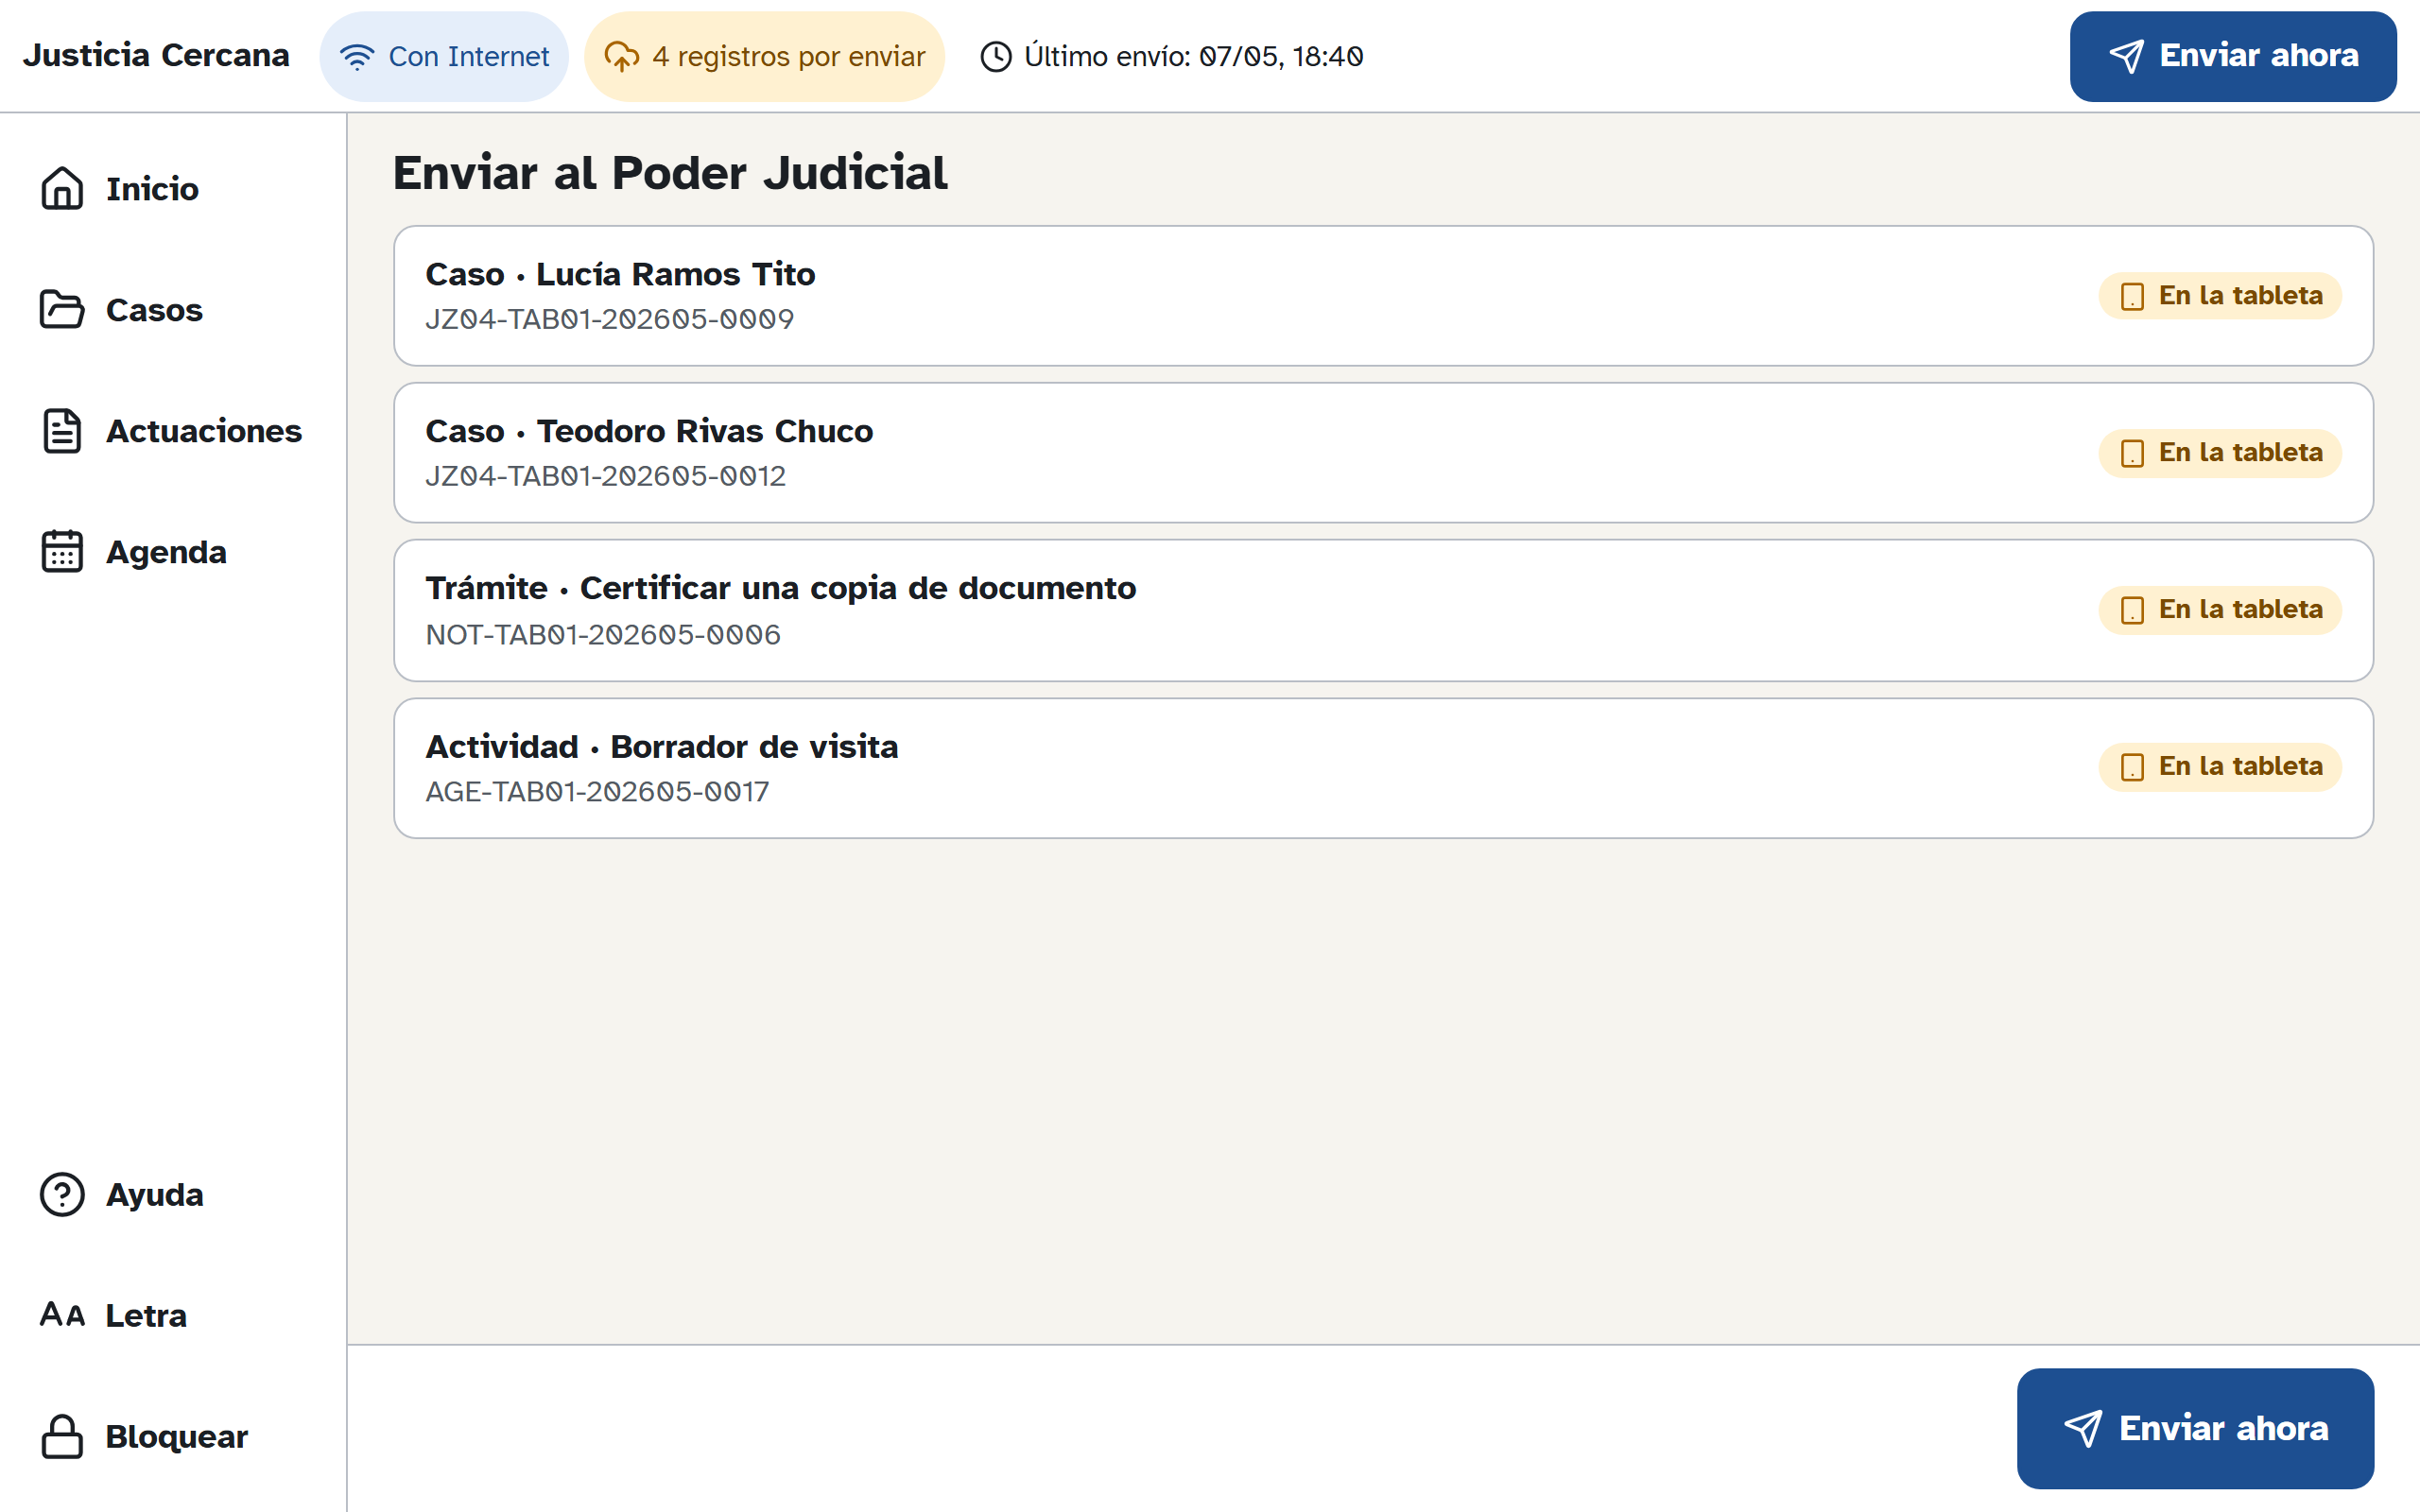
\includegraphics[width=\linewidth]{../../captures/P-09_envio.png}\\[-2pt]{\footnotesize\raggedright\textbf{P-09.} Envío al Poder Judicial: registros por enviar con distintivo y [Enviar ahora] \emph{(Funcionamiento sin conexión)}\par}\end{minipage}\hfill
\begin{minipage}[t]{0.49\textwidth}\centering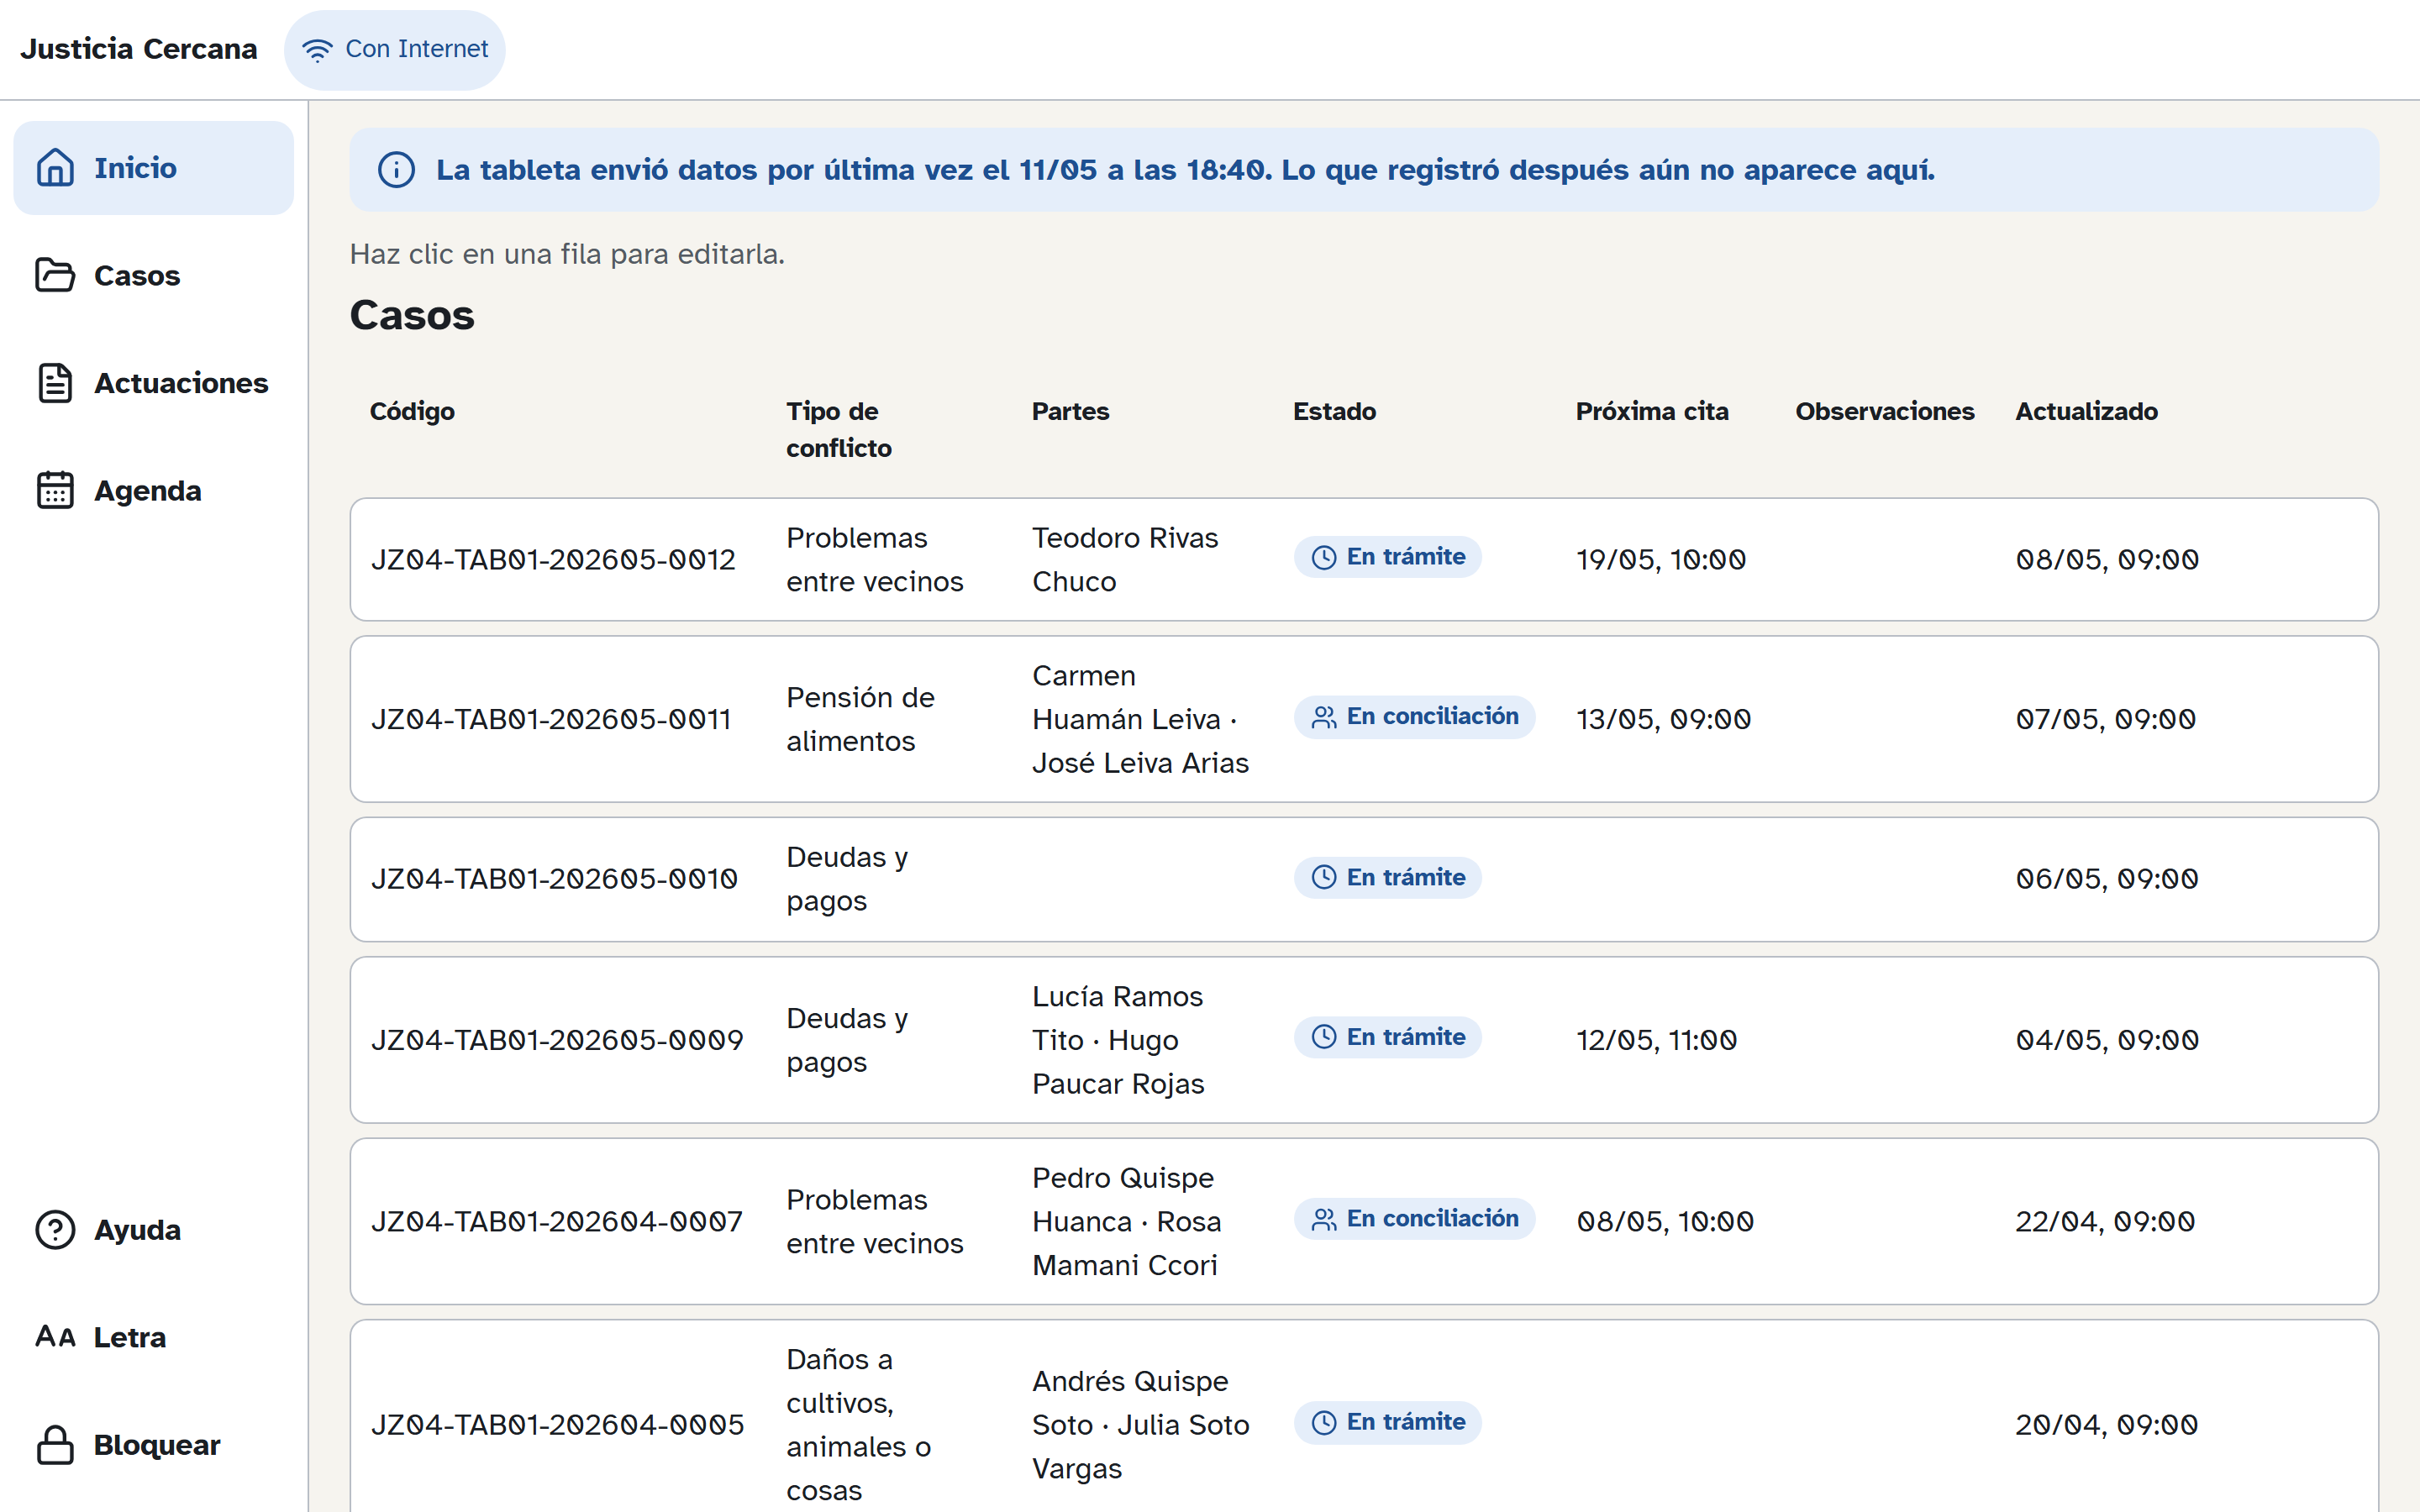
\includegraphics[width=\linewidth]{../../captures/P-10_computadora.png}\\[-2pt]{\footnotesize\raggedright\textbf{P-10.} Vista en computadora 1440×900: tablas con más columnas, aviso del último envío \emph{(Cobertura y funcionamiento de los módulos)}\par}\end{minipage}\par\vspace{8pt}\noindent
\par\vspace{4pt}
\subsection*{Flujo 1}
\noindent
\begin{minipage}[t]{0.49\textwidth}\centering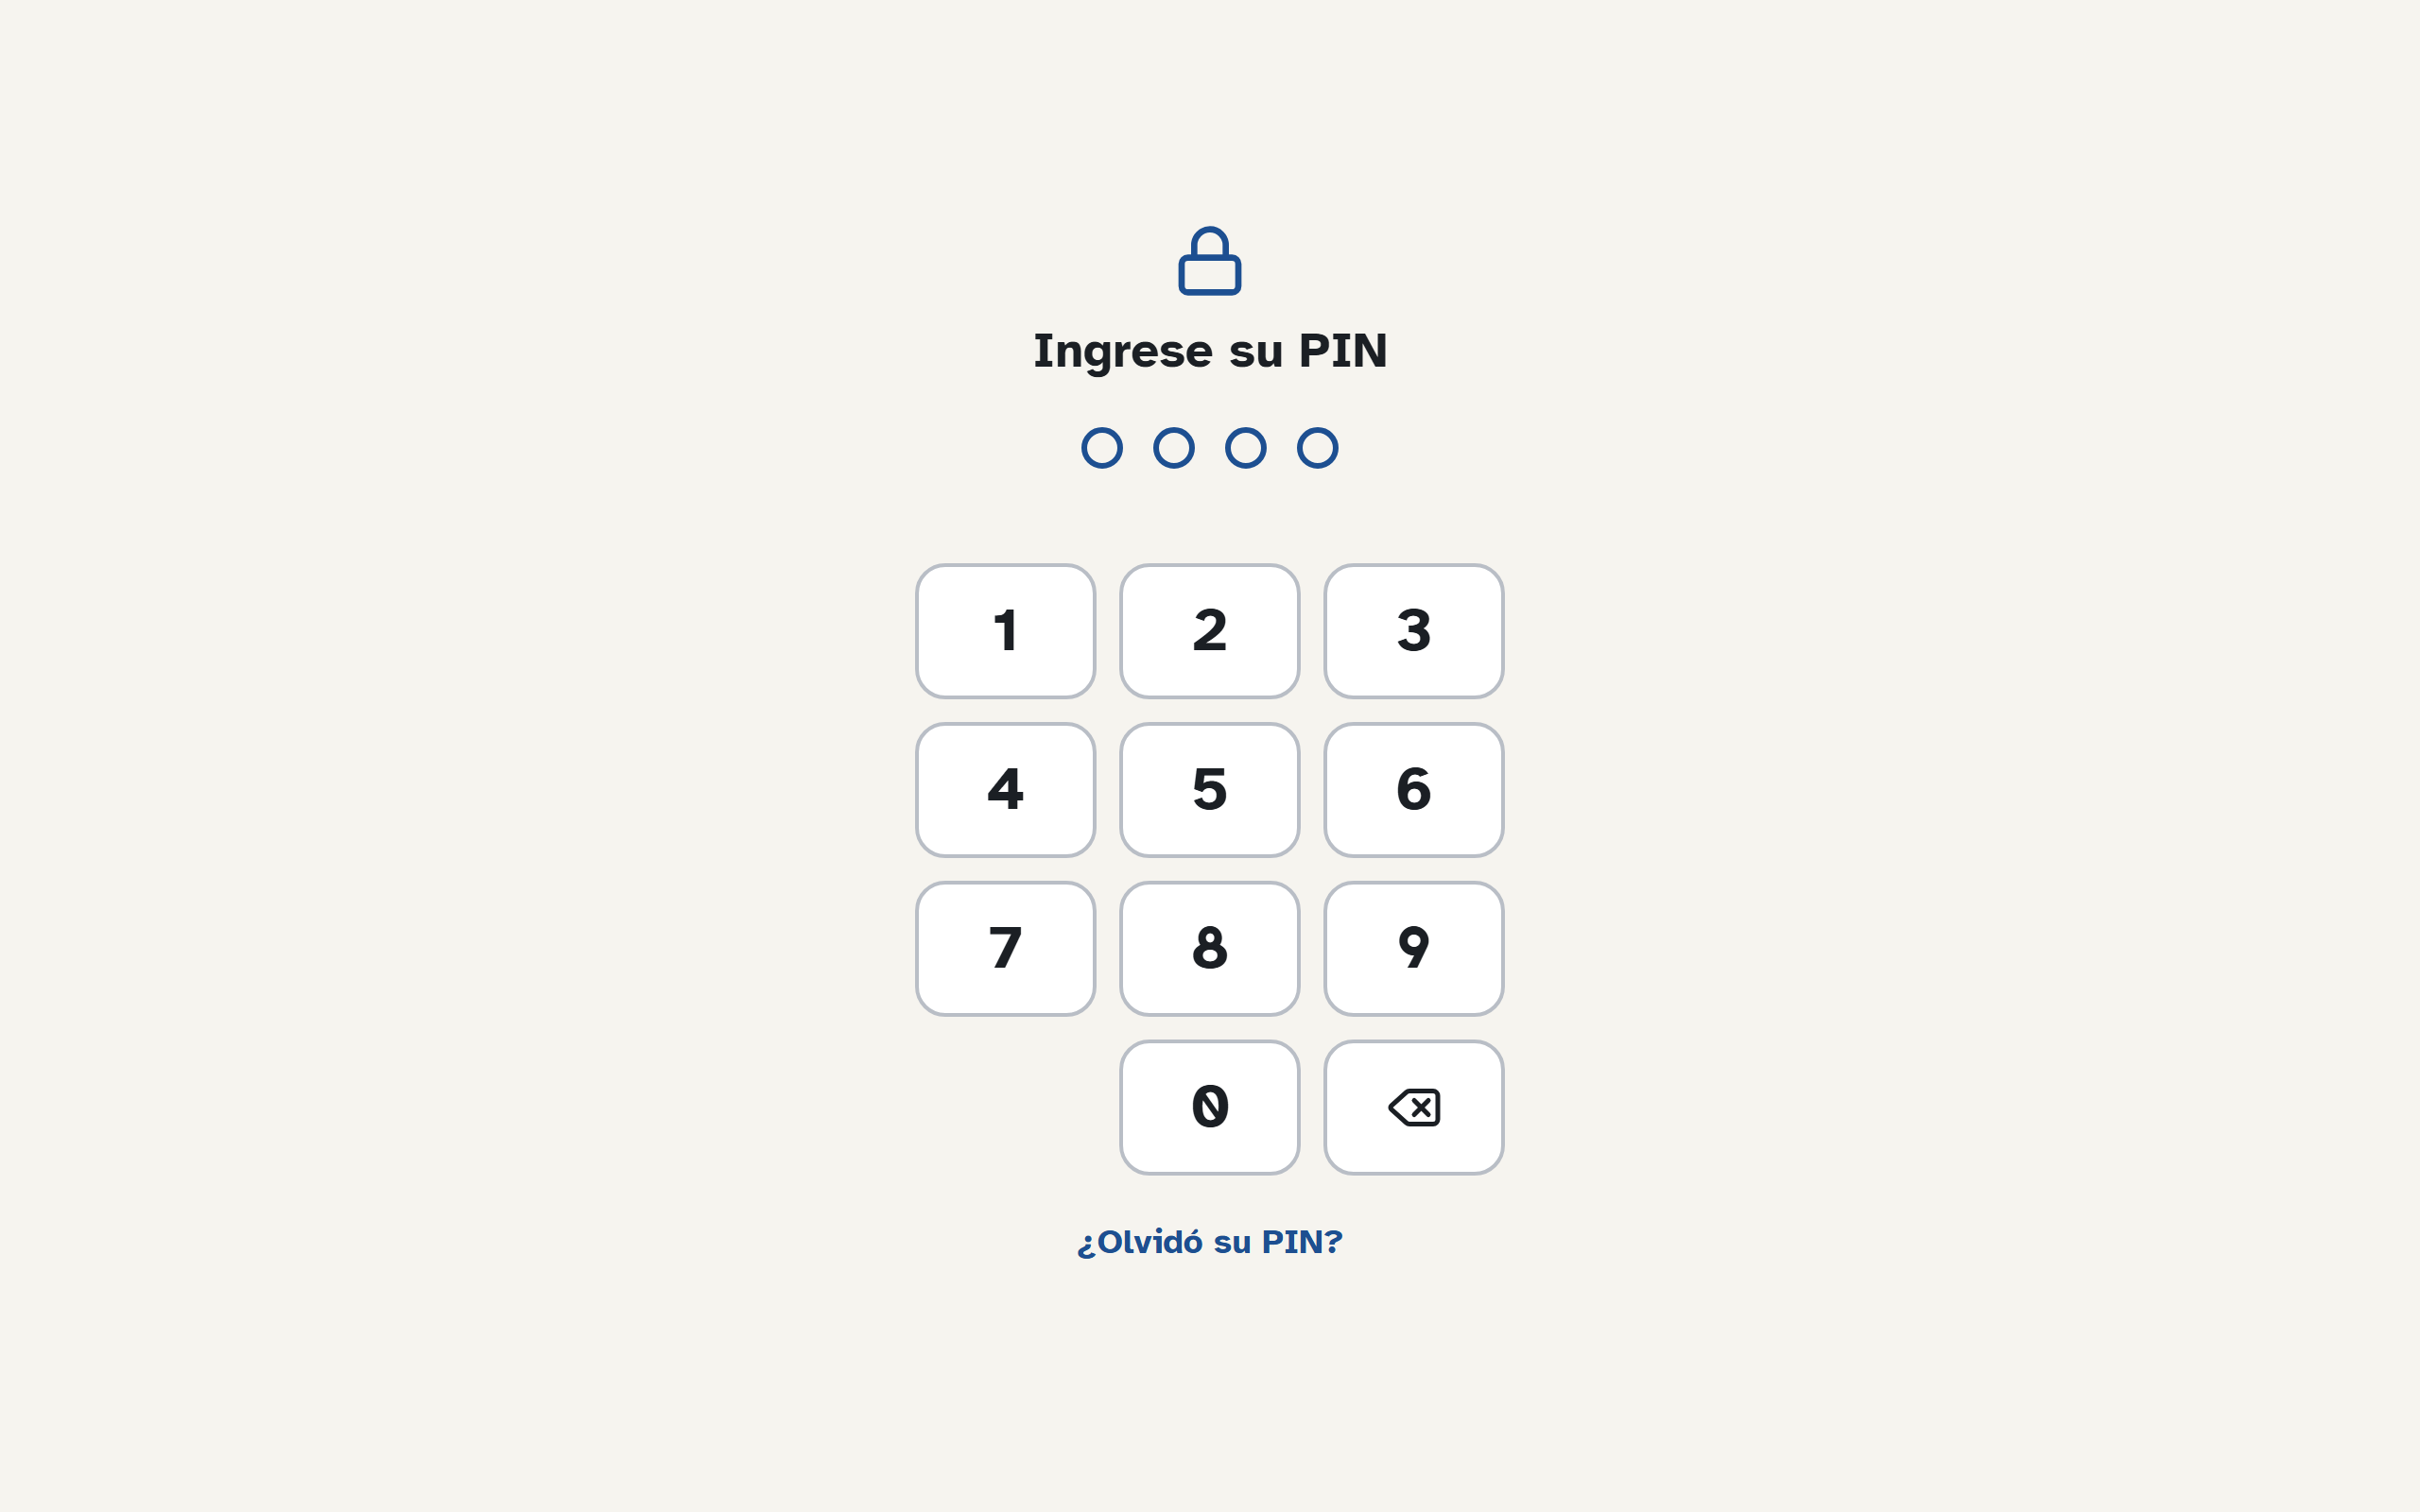
\includegraphics[width=\linewidth]{../../captures/F1-01a_pin.png}\\[-2pt]{\footnotesize\raggedright\textbf{P-00 · 1.} Ingreso con PIN numérico y teclado grande; funciona sin Internet \emph{(Factores humanos y dispositivo)}\par}\end{minipage}\hfill
\begin{minipage}[t]{0.49\textwidth}\centering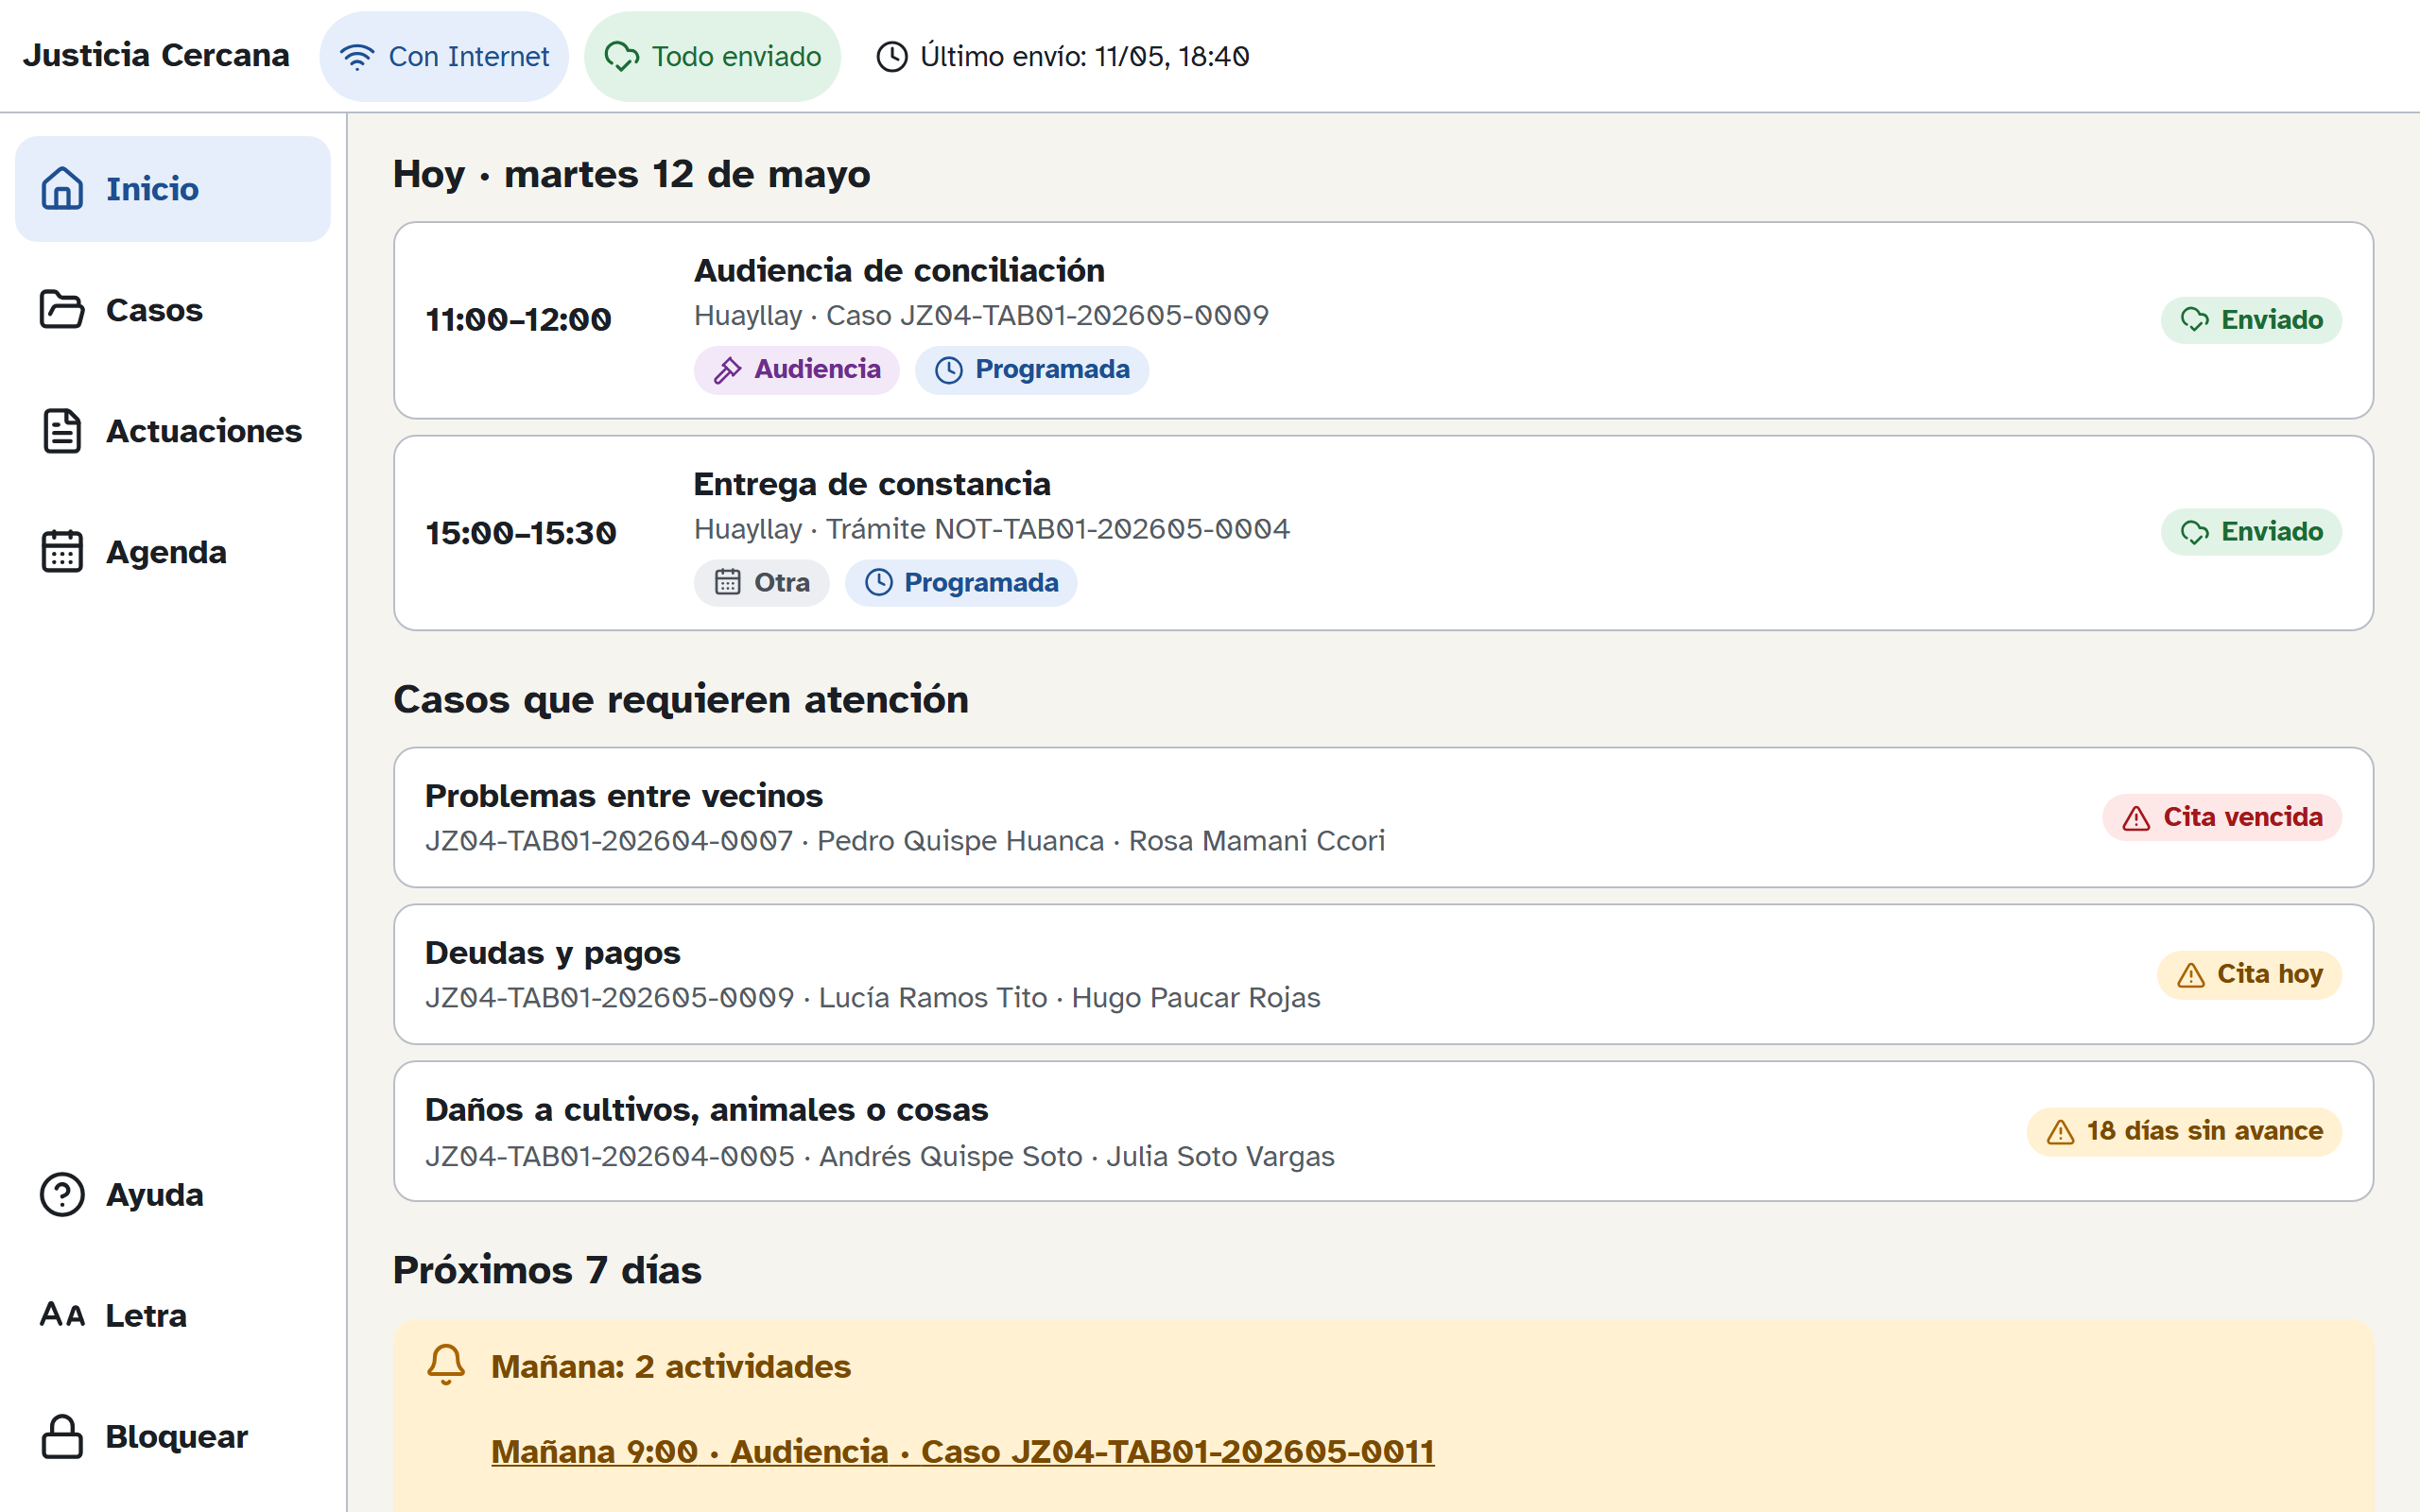
\includegraphics[width=\linewidth]{../../captures/F1-01b_inicio-con-internet.png}\\[-2pt]{\footnotesize\raggedright\textbf{P-01 · 1.} Inicio con barra ``Con Internet'' · ``Todo enviado'' \emph{(Funcionamiento sin conexión)}\par}\end{minipage}\par\vspace{8pt}\noindent
\begin{minipage}[t]{0.49\textwidth}\centering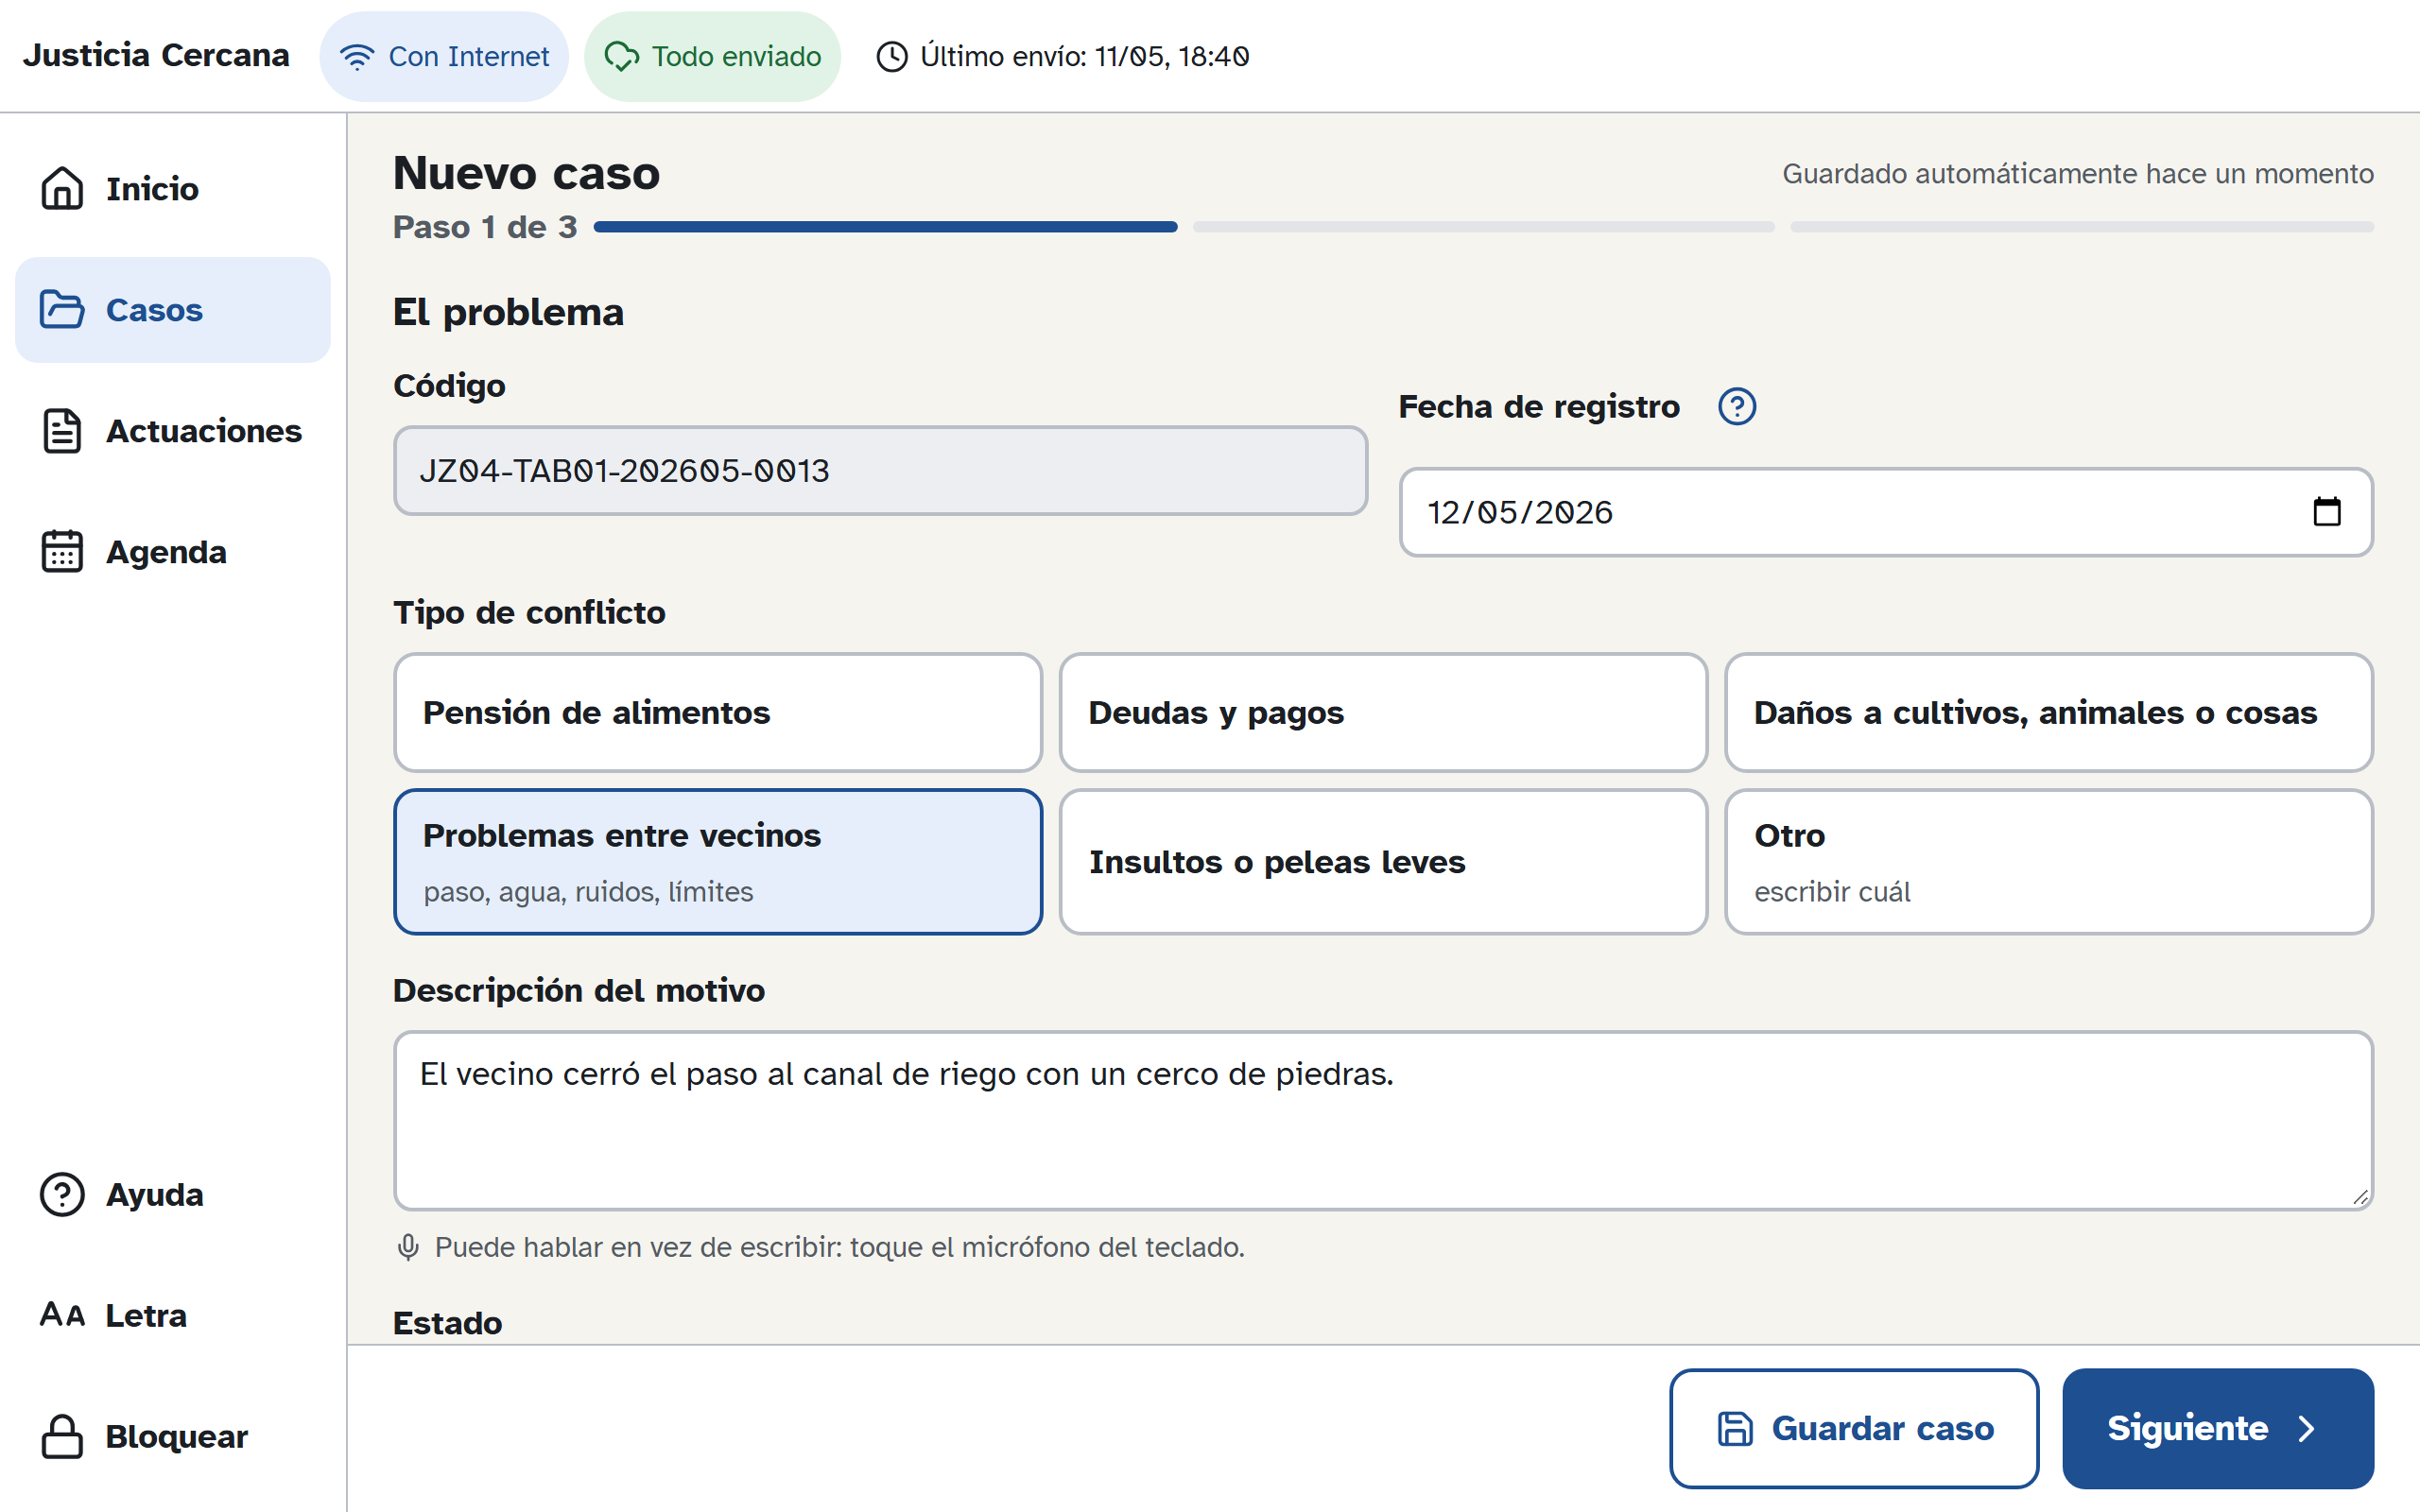
\includegraphics[width=\linewidth]{../../captures/F1-02_nuevo-caso-paso1.png}\\[-2pt]{\footnotesize\raggedright\textbf{P-03 · 2.} Paso 1 ``El problema'': tipo con botones grandes, descripción con ayuda de dictado y guardado automático \emph{(Cobertura y funcionamiento de los módulos)}\par}\end{minipage}\hfill
\begin{minipage}[t]{0.49\textwidth}\centering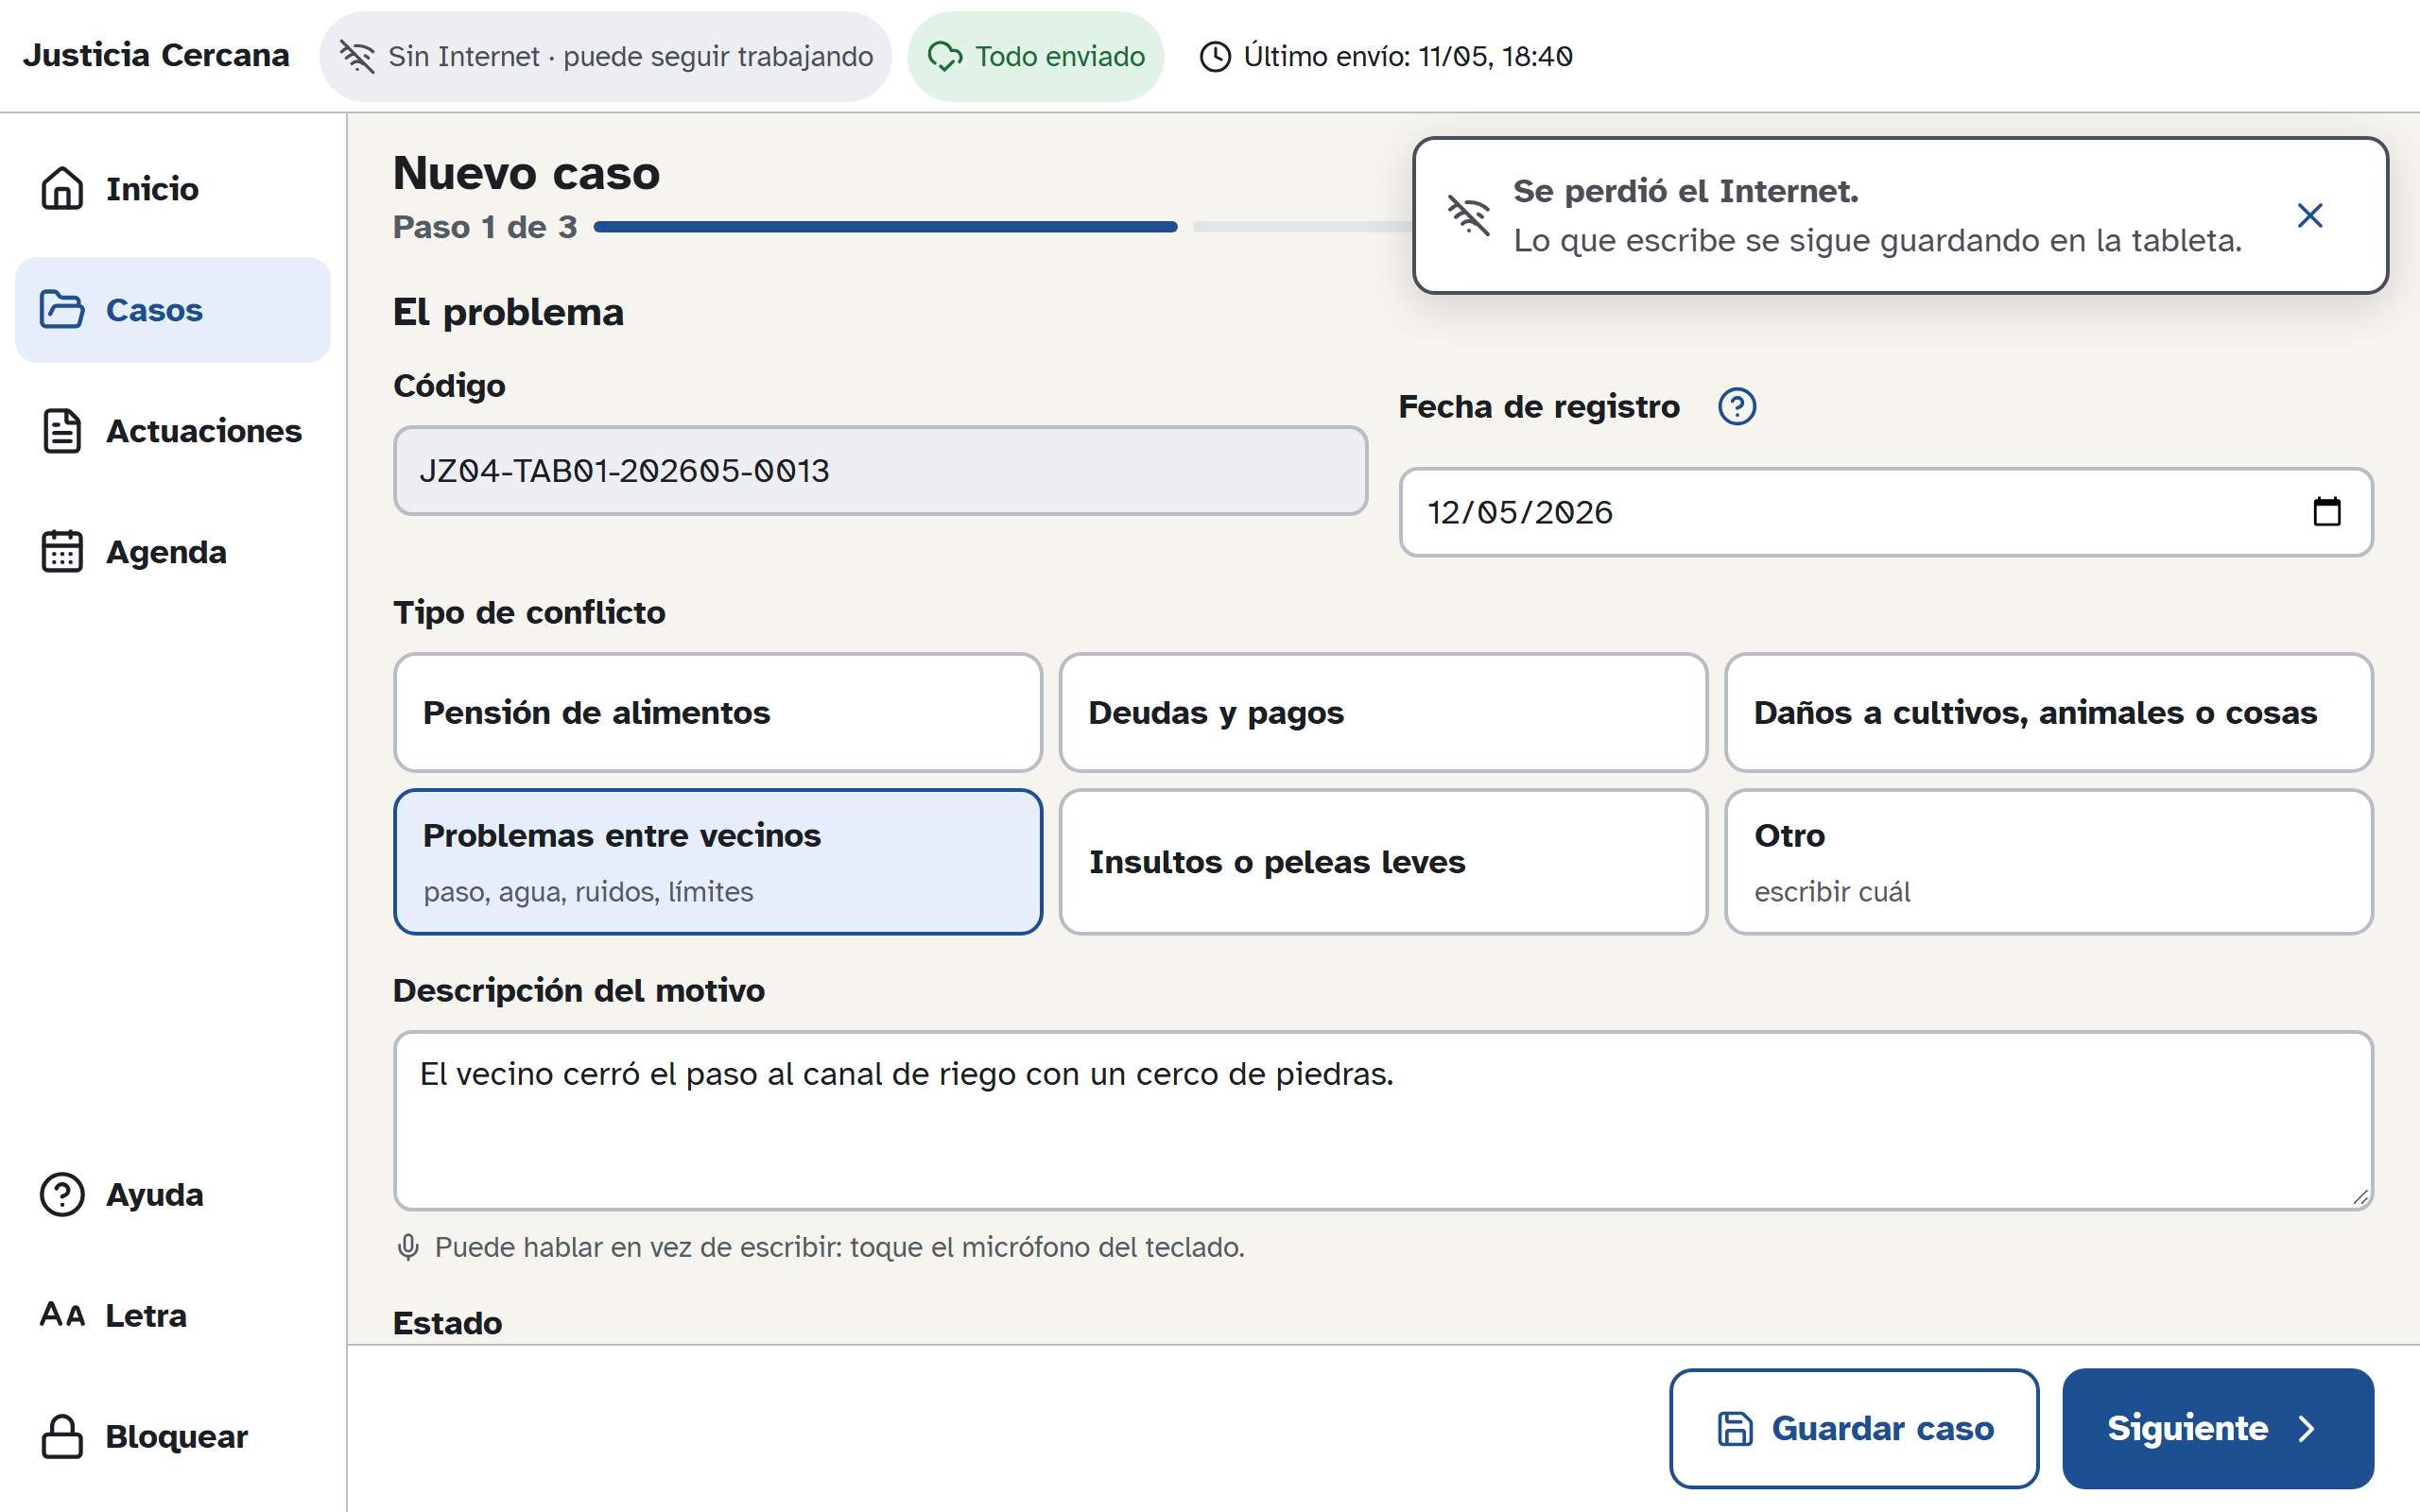
\includegraphics[width=\linewidth]{../../captures/F1-03_aviso-corte-internet.png}\\[-2pt]{\footnotesize\raggedright\textbf{P-03 · 3.} Corte real de Internet a mitad del formulario: aviso gris y barra ``Sin Internet'' \emph{(Funcionamiento sin conexión)}\par}\end{minipage}\par\vspace{8pt}\noindent
\begin{minipage}[t]{0.49\textwidth}\centering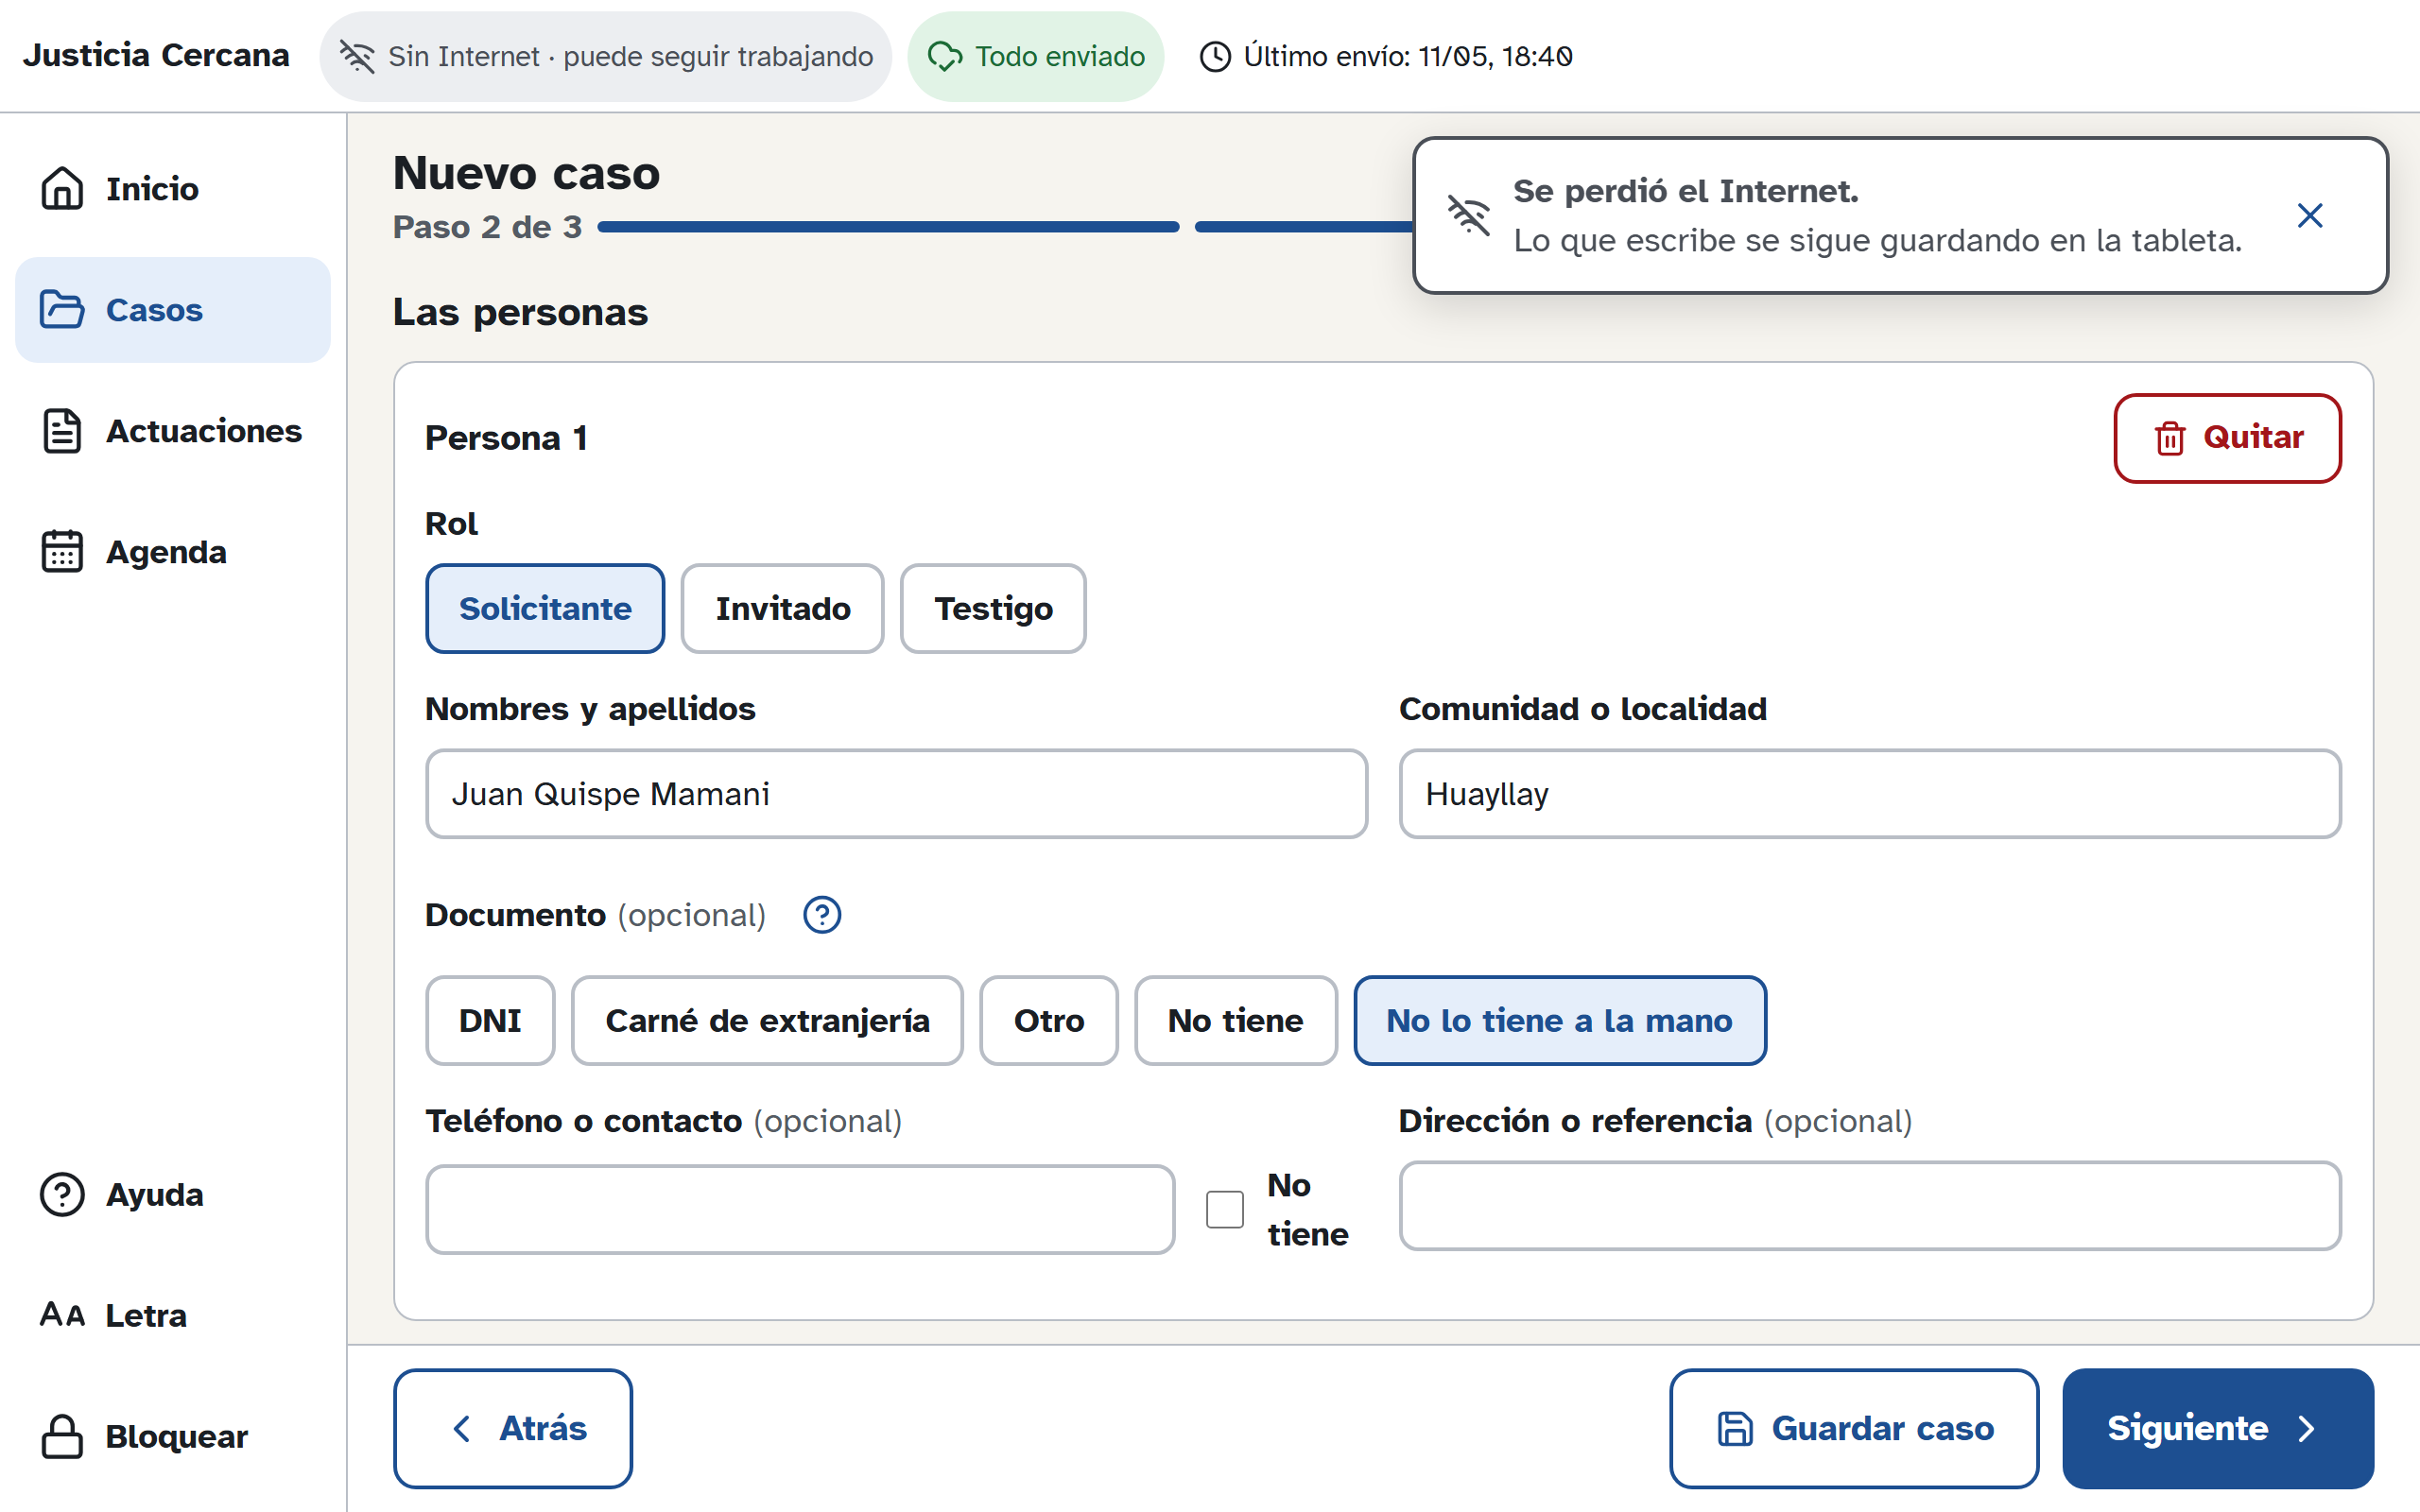
\includegraphics[width=\linewidth]{../../captures/F1-04_parte1-solicitante.png}\\[-2pt]{\footnotesize\raggedright\textbf{P-03 · 4.} Parte 1 con rol, patrón ``No lo tiene a la mano'' y comunidad, sin Internet \emph{(Cobertura y funcionamiento de los módulos)}\par}\end{minipage}\hfill
\begin{minipage}[t]{0.49\textwidth}\centering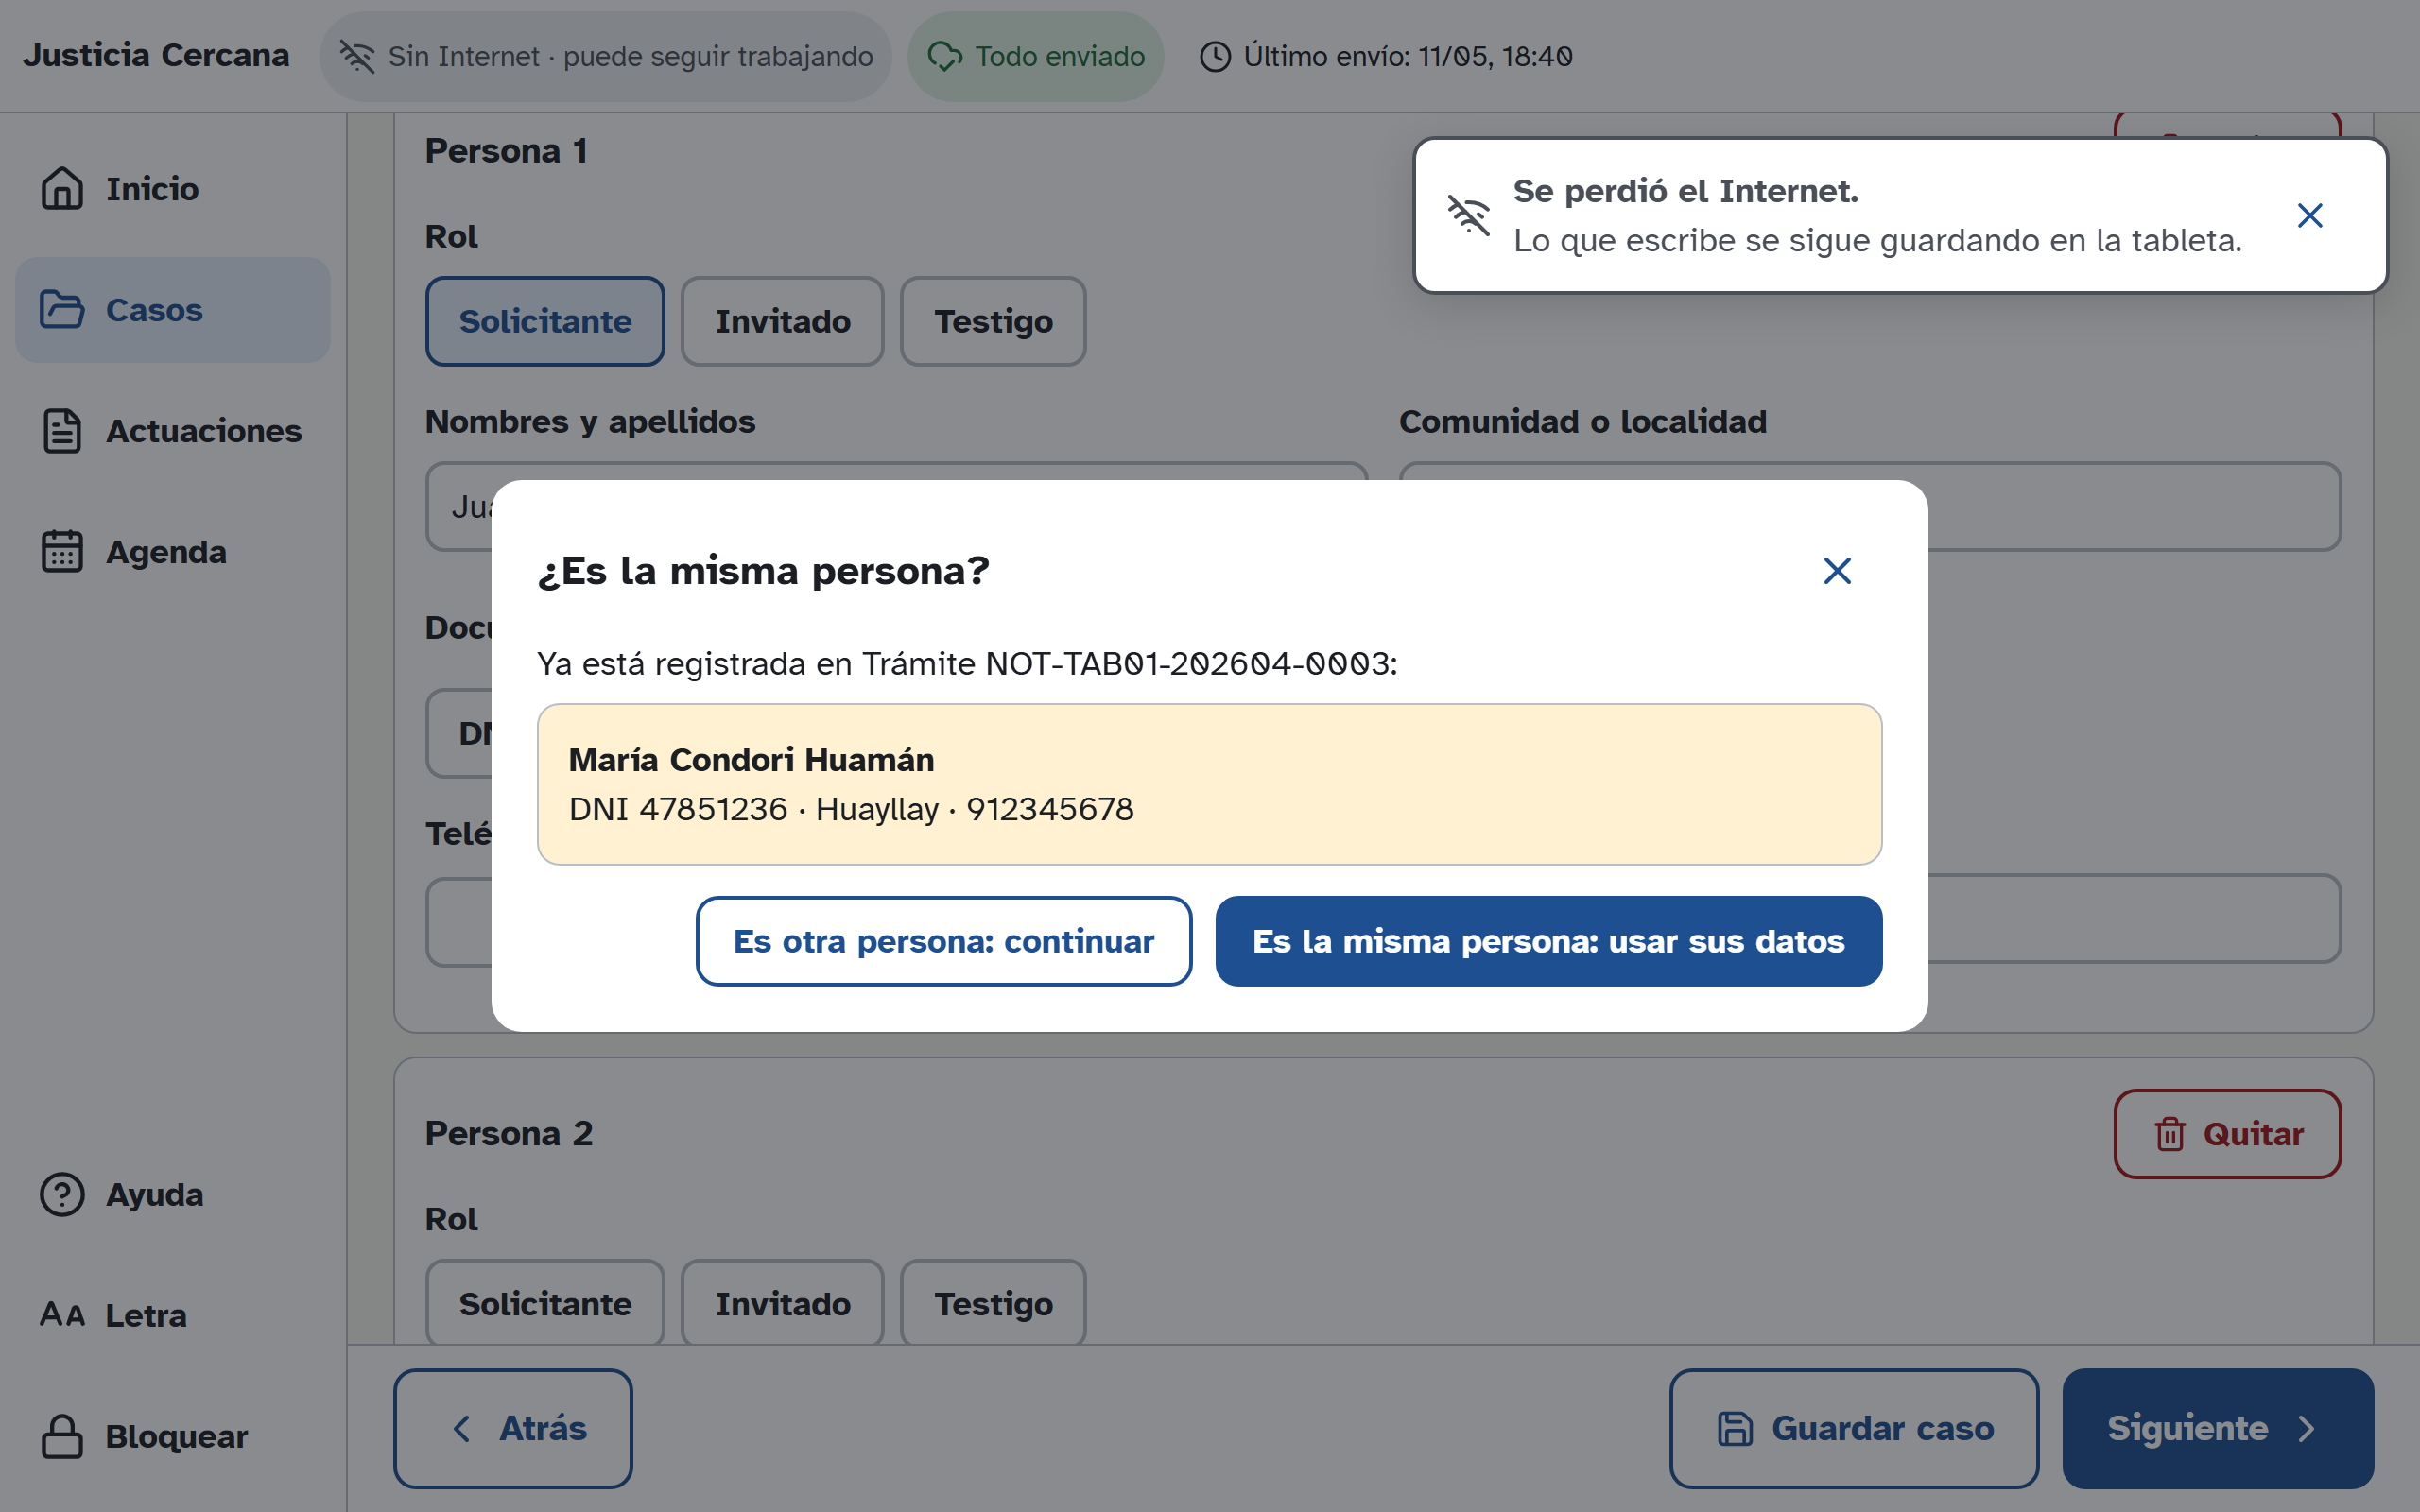
\includegraphics[width=\linewidth]{../../captures/F1-05a_advertencia-duplicado.png}\\[-2pt]{\footnotesize\raggedright\textbf{P-03 · 5.} Advertencia de duplicado (regla 5.3) que no bloquea \emph{(Principios de diseño y heurísticas)}\par}\end{minipage}\par\vspace{8pt}\noindent
\begin{minipage}[t]{0.49\textwidth}\centering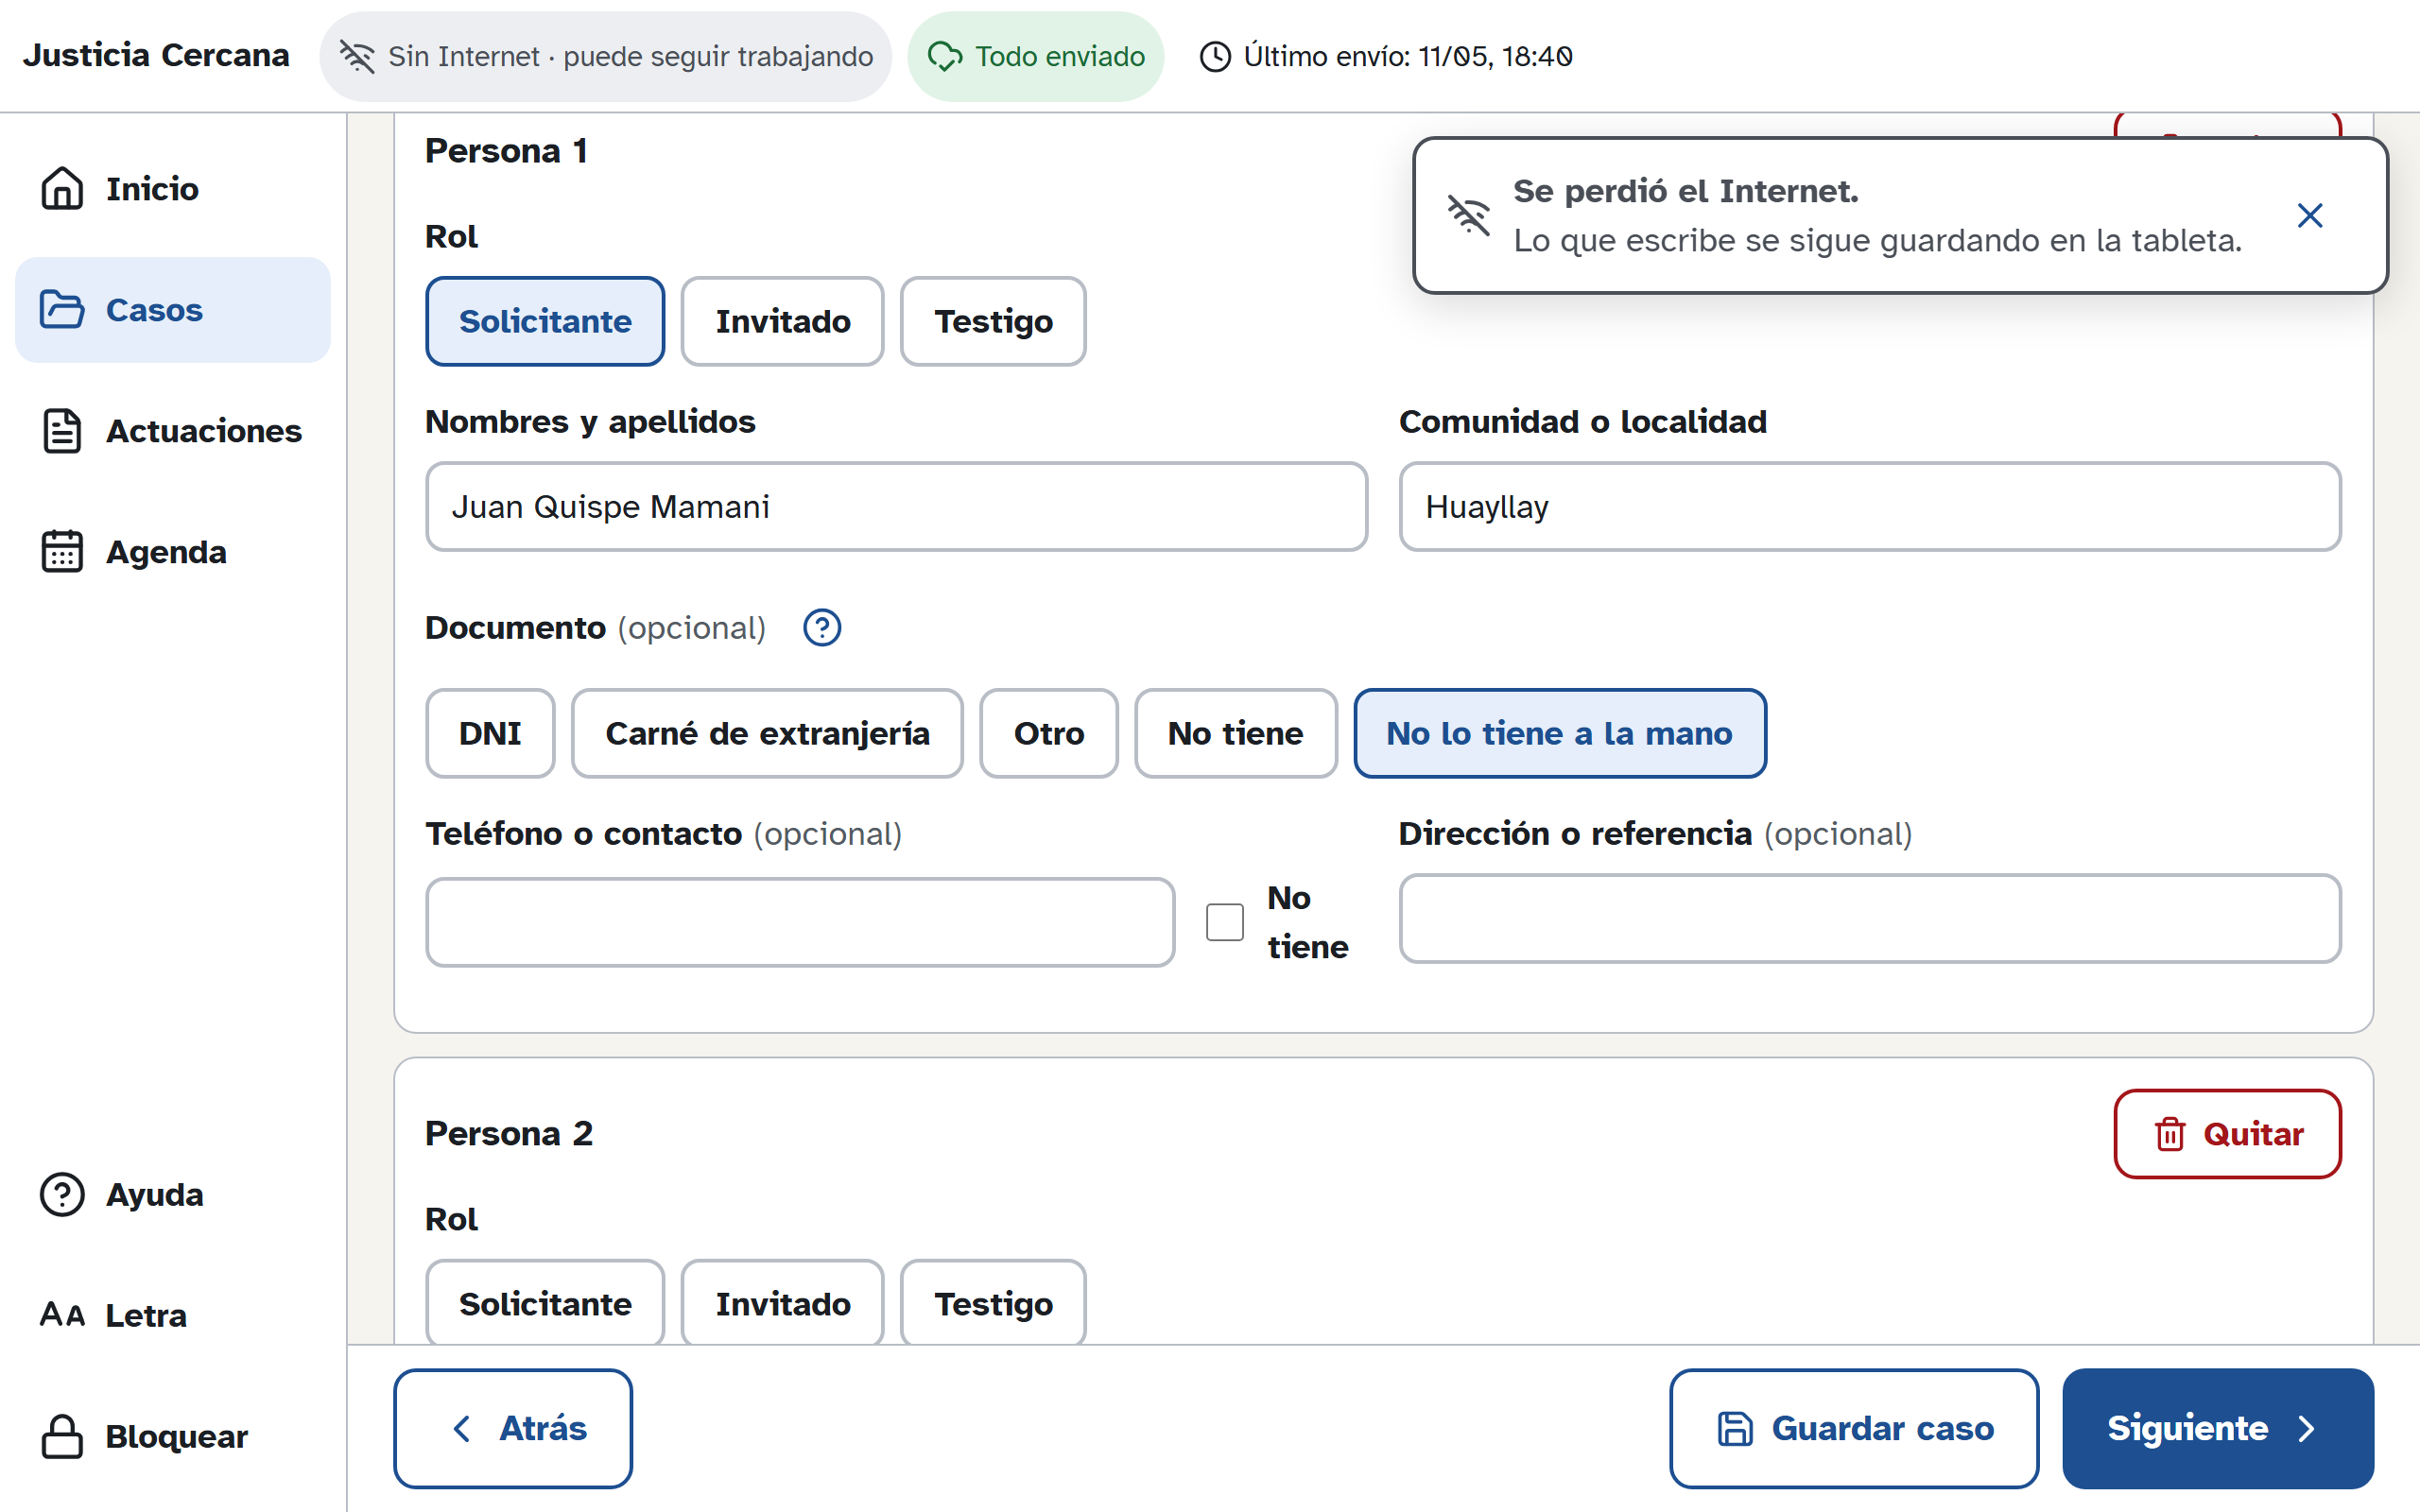
\includegraphics[width=\linewidth]{../../captures/F1-05b_datos-reutilizados.png}\\[-2pt]{\footnotesize\raggedright\textbf{P-03 · 5.} Se reutilizan los datos de la persona ya registrada \emph{(Principios de diseño y heurísticas)}\par}\end{minipage}\hfill
\begin{minipage}[t]{0.49\textwidth}\centering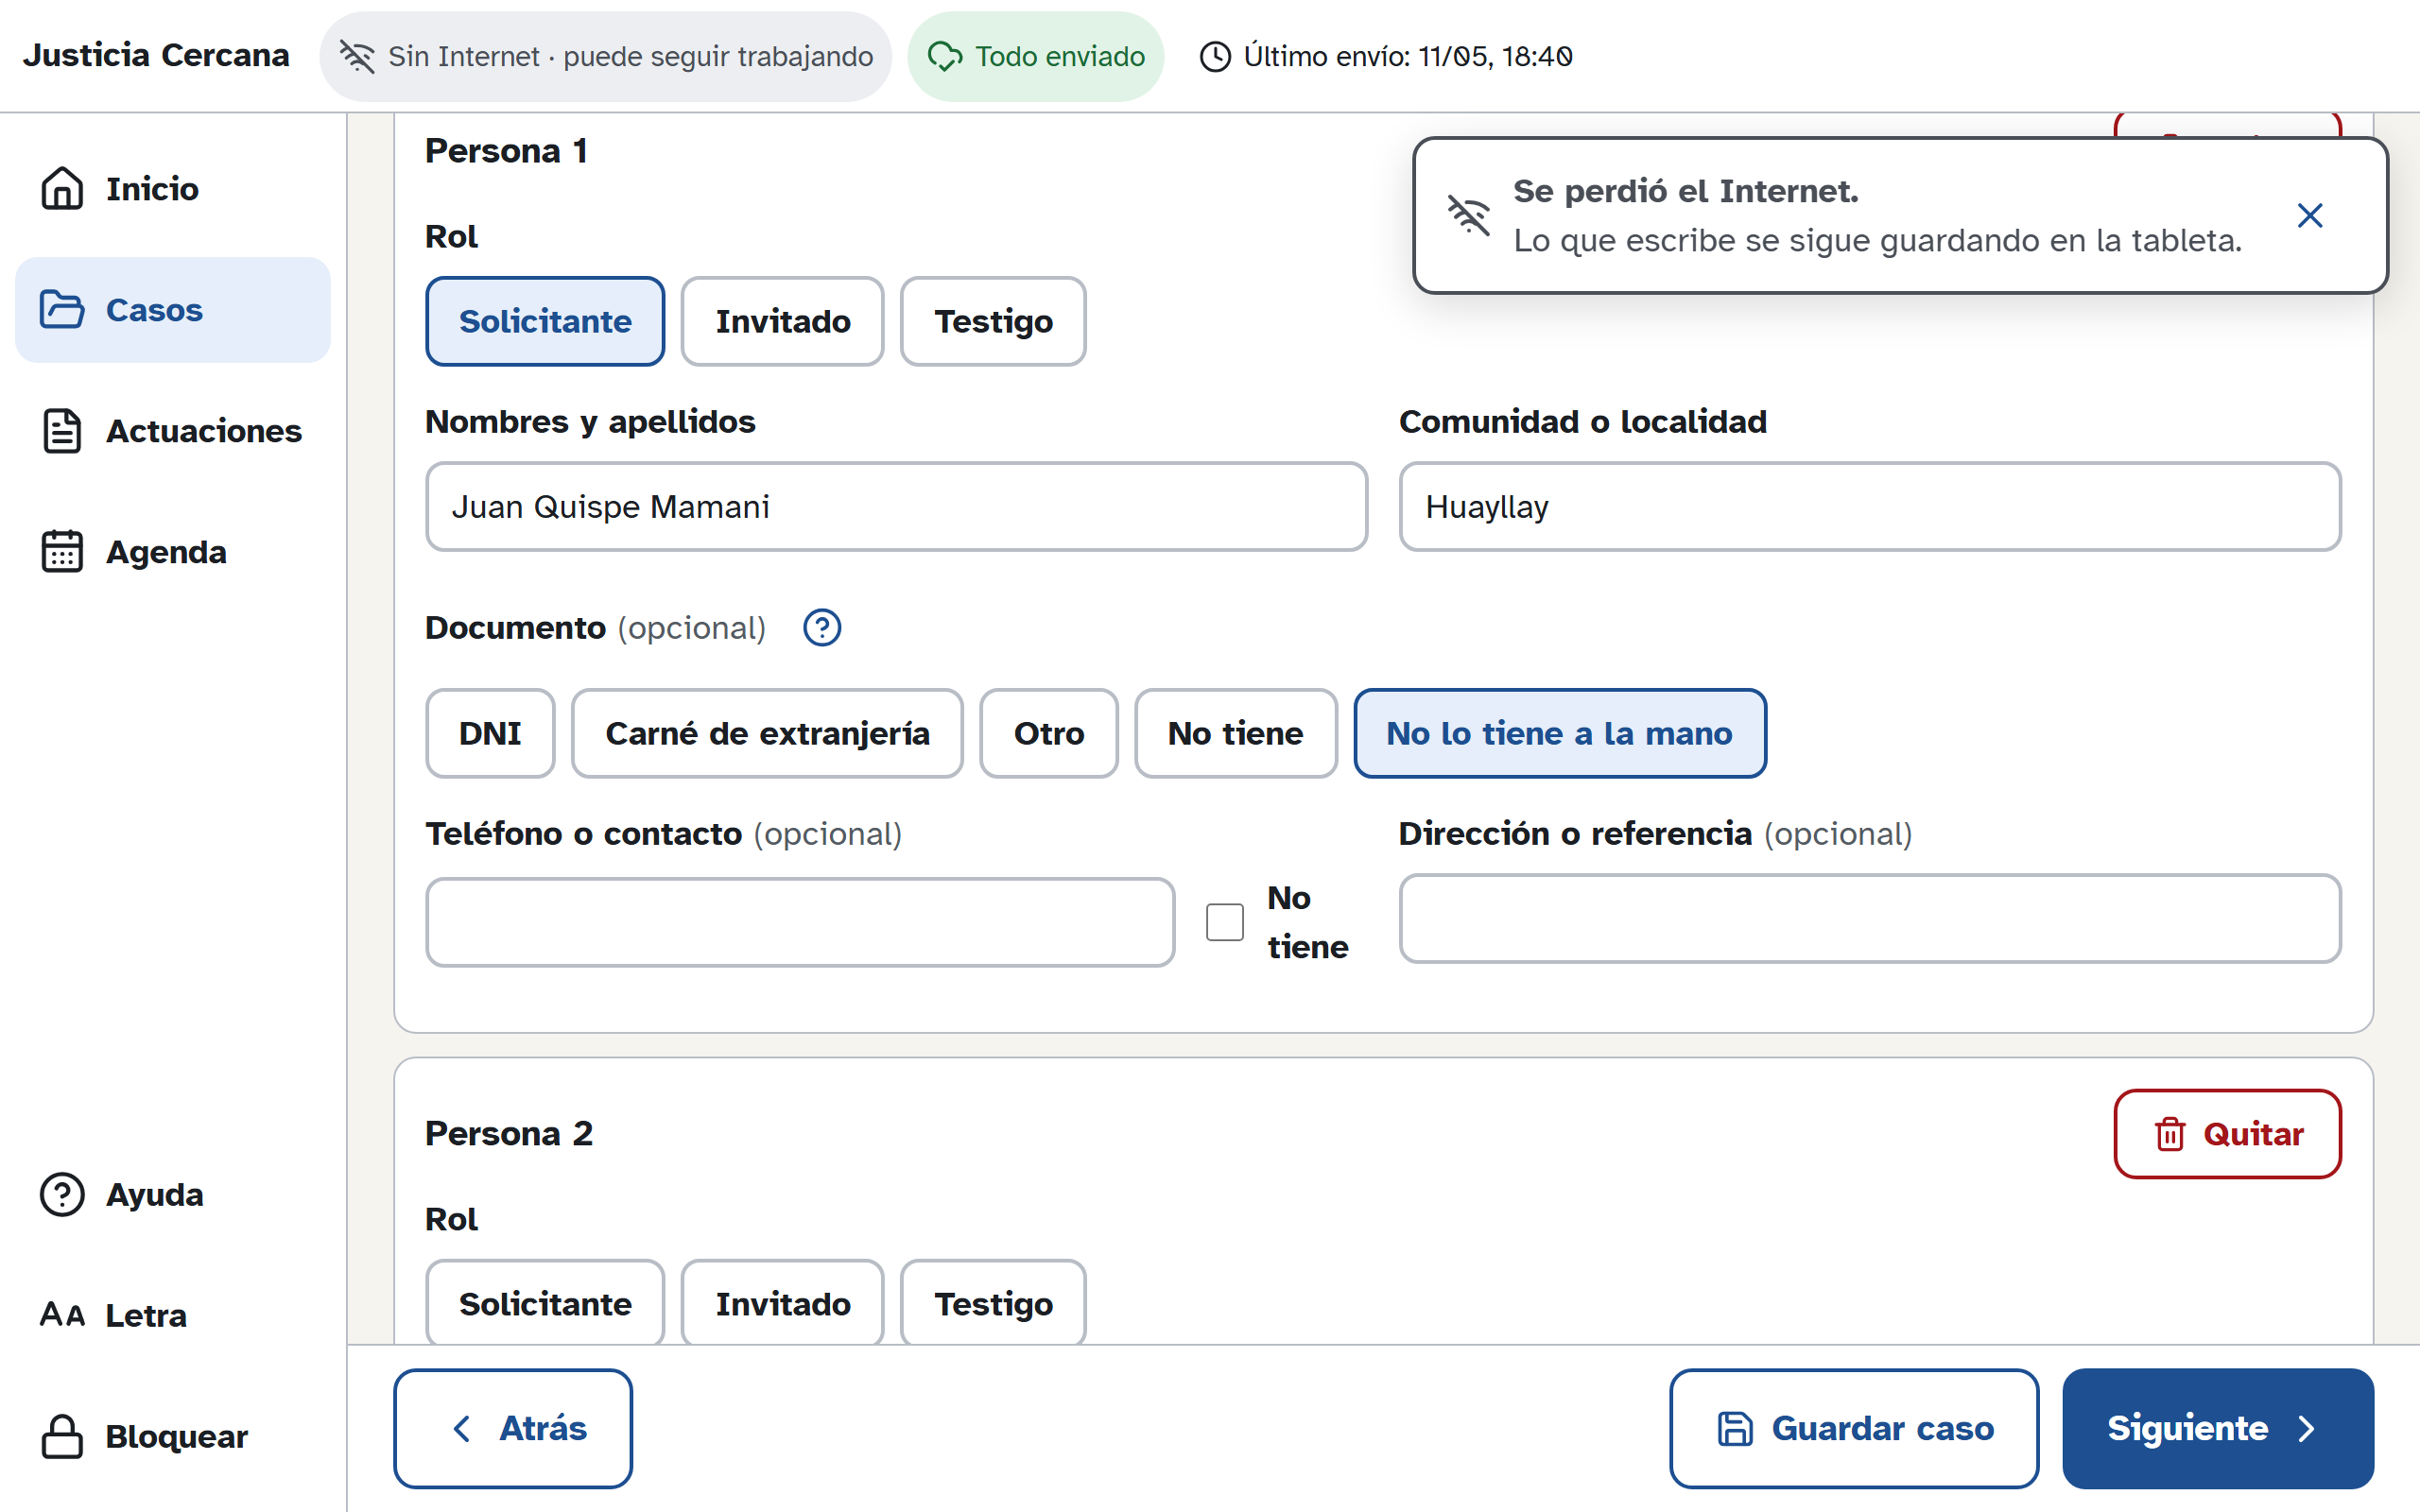
\includegraphics[width=\linewidth]{../../captures/F1-06_error-sin-rol.png}\\[-2pt]{\footnotesize\raggedright\textbf{P-03 · 6.} Error de validación en lenguaje simple junto al campo \emph{(Principios de diseño y heurísticas)}\par}\end{minipage}\par\vspace{8pt}\noindent
\begin{minipage}[t]{0.49\textwidth}\centering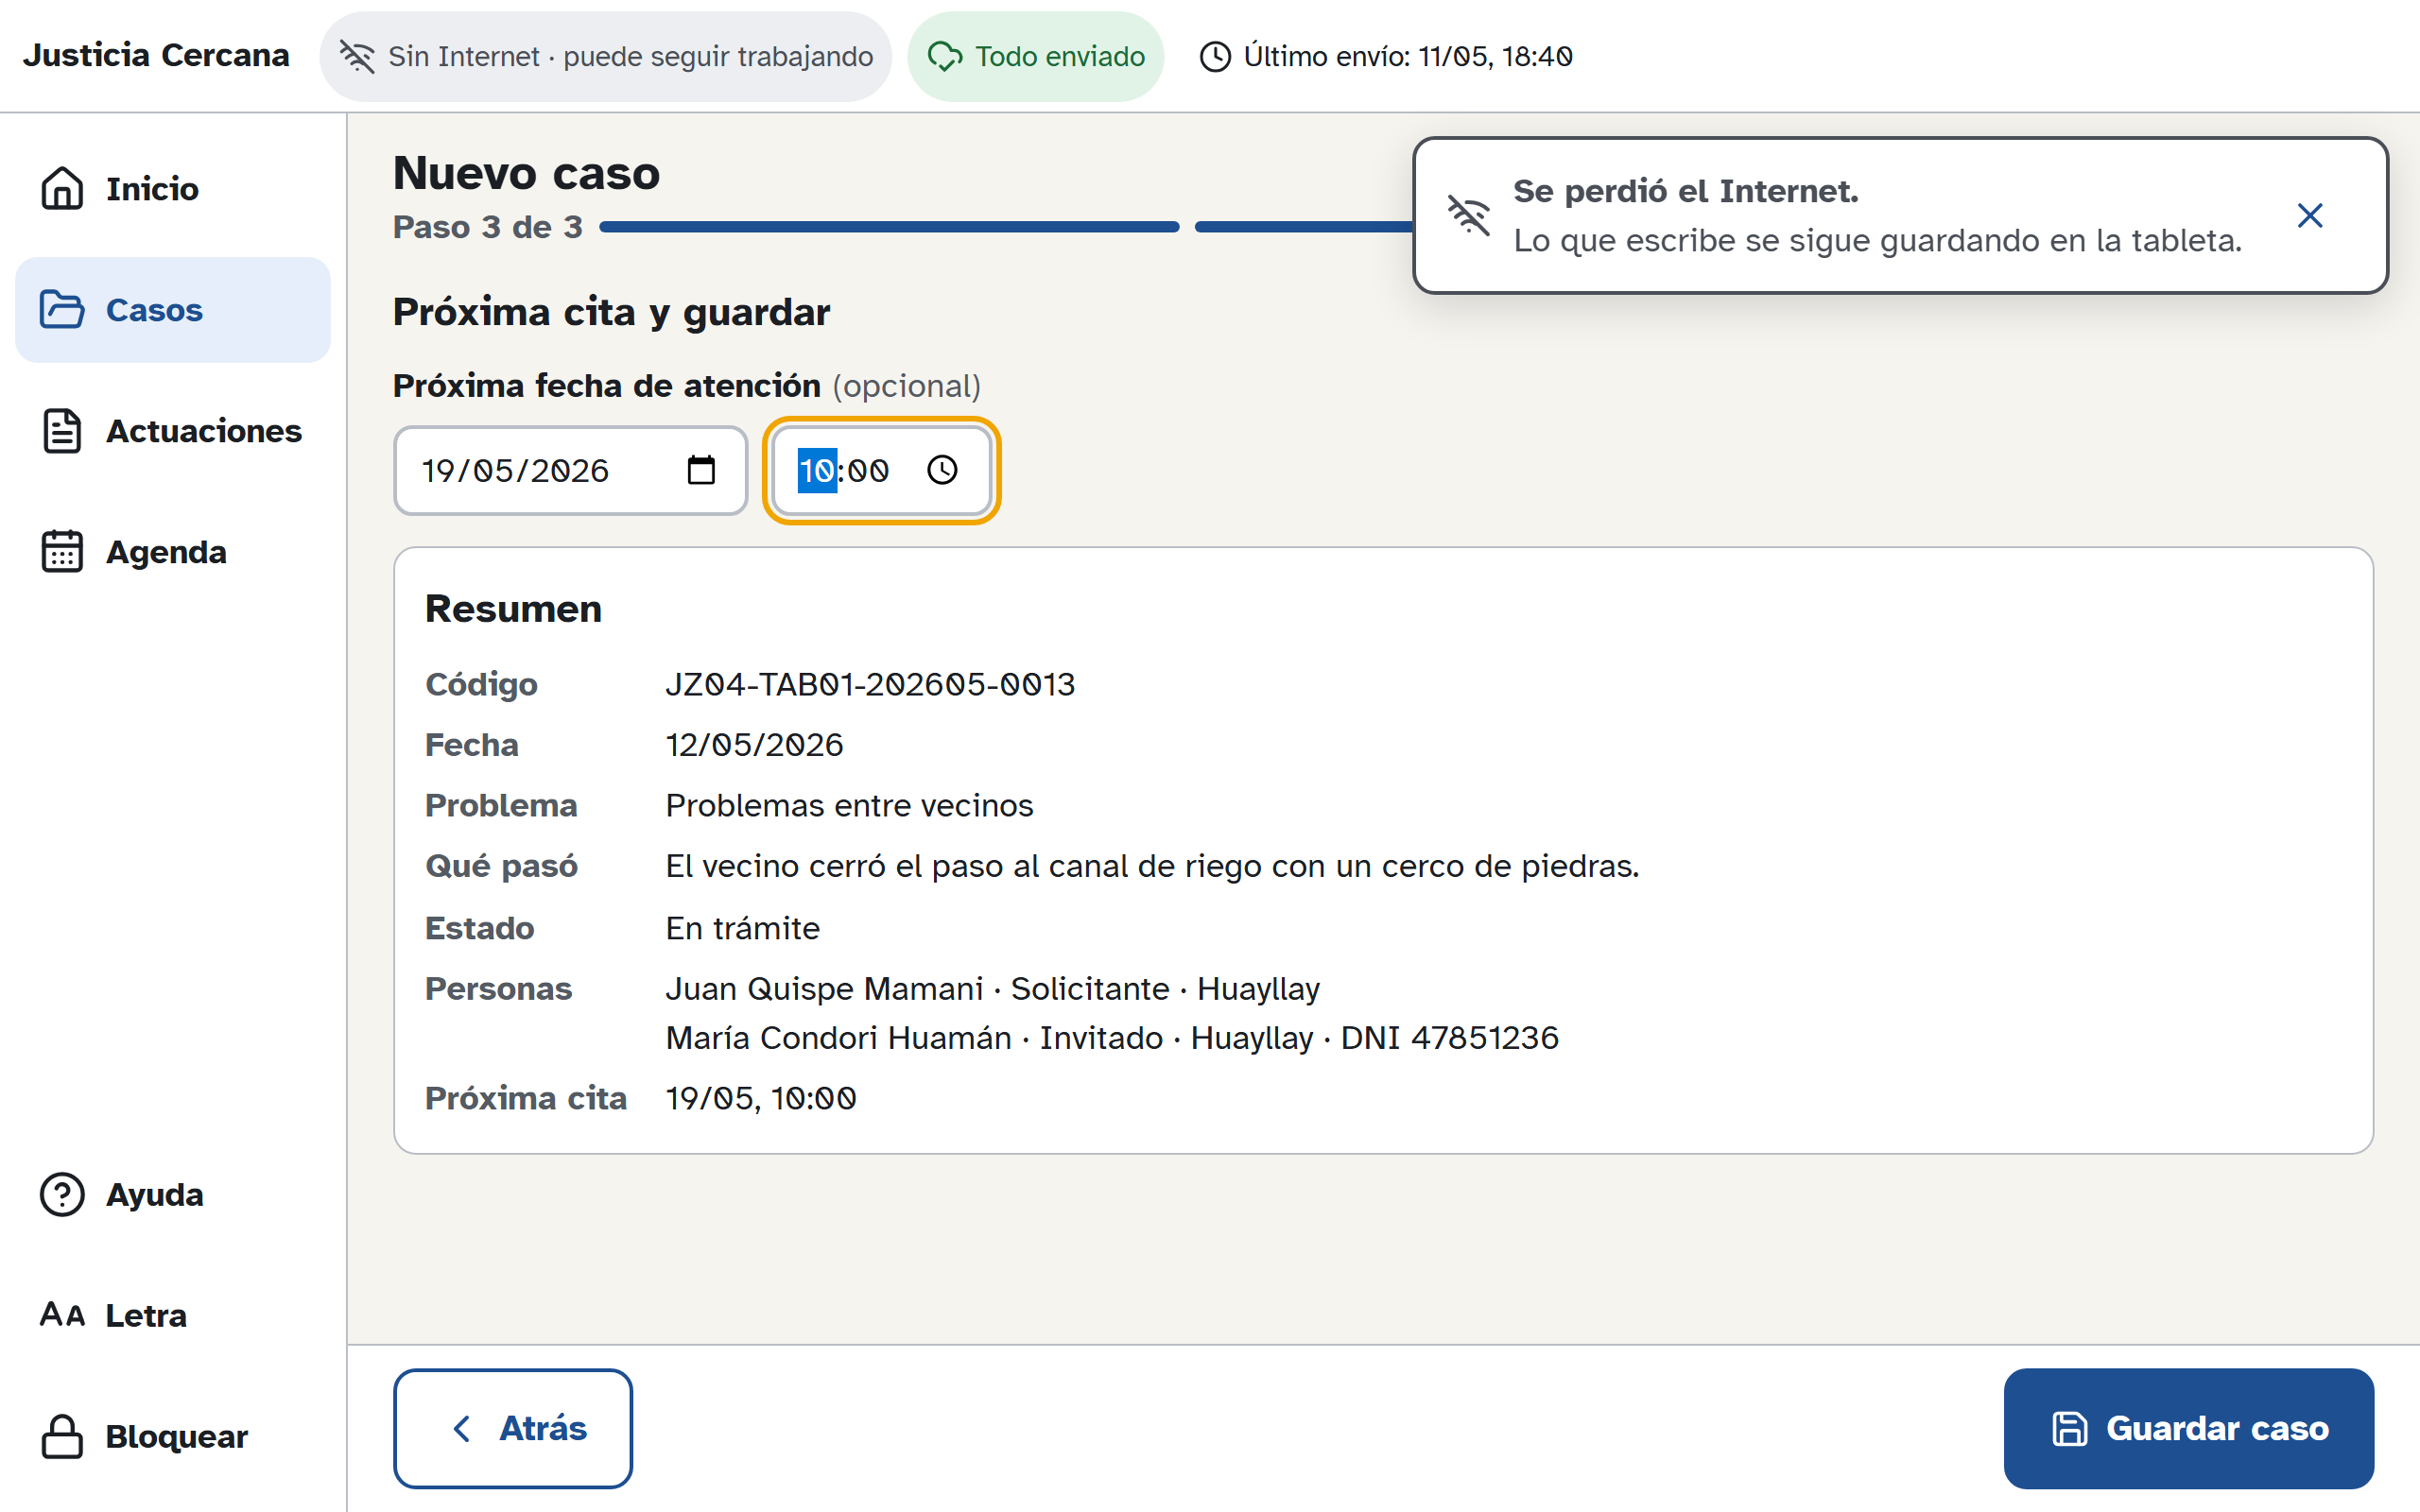
\includegraphics[width=\linewidth]{../../captures/F1-07_resumen-proxima-cita.png}\\[-2pt]{\footnotesize\raggedright\textbf{P-03 · 7.} Próxima cita 19/05 10:00 y resumen legible antes de guardar \emph{(Cobertura y funcionamiento de los módulos)}\par}\end{minipage}\hfill
\begin{minipage}[t]{0.49\textwidth}\centering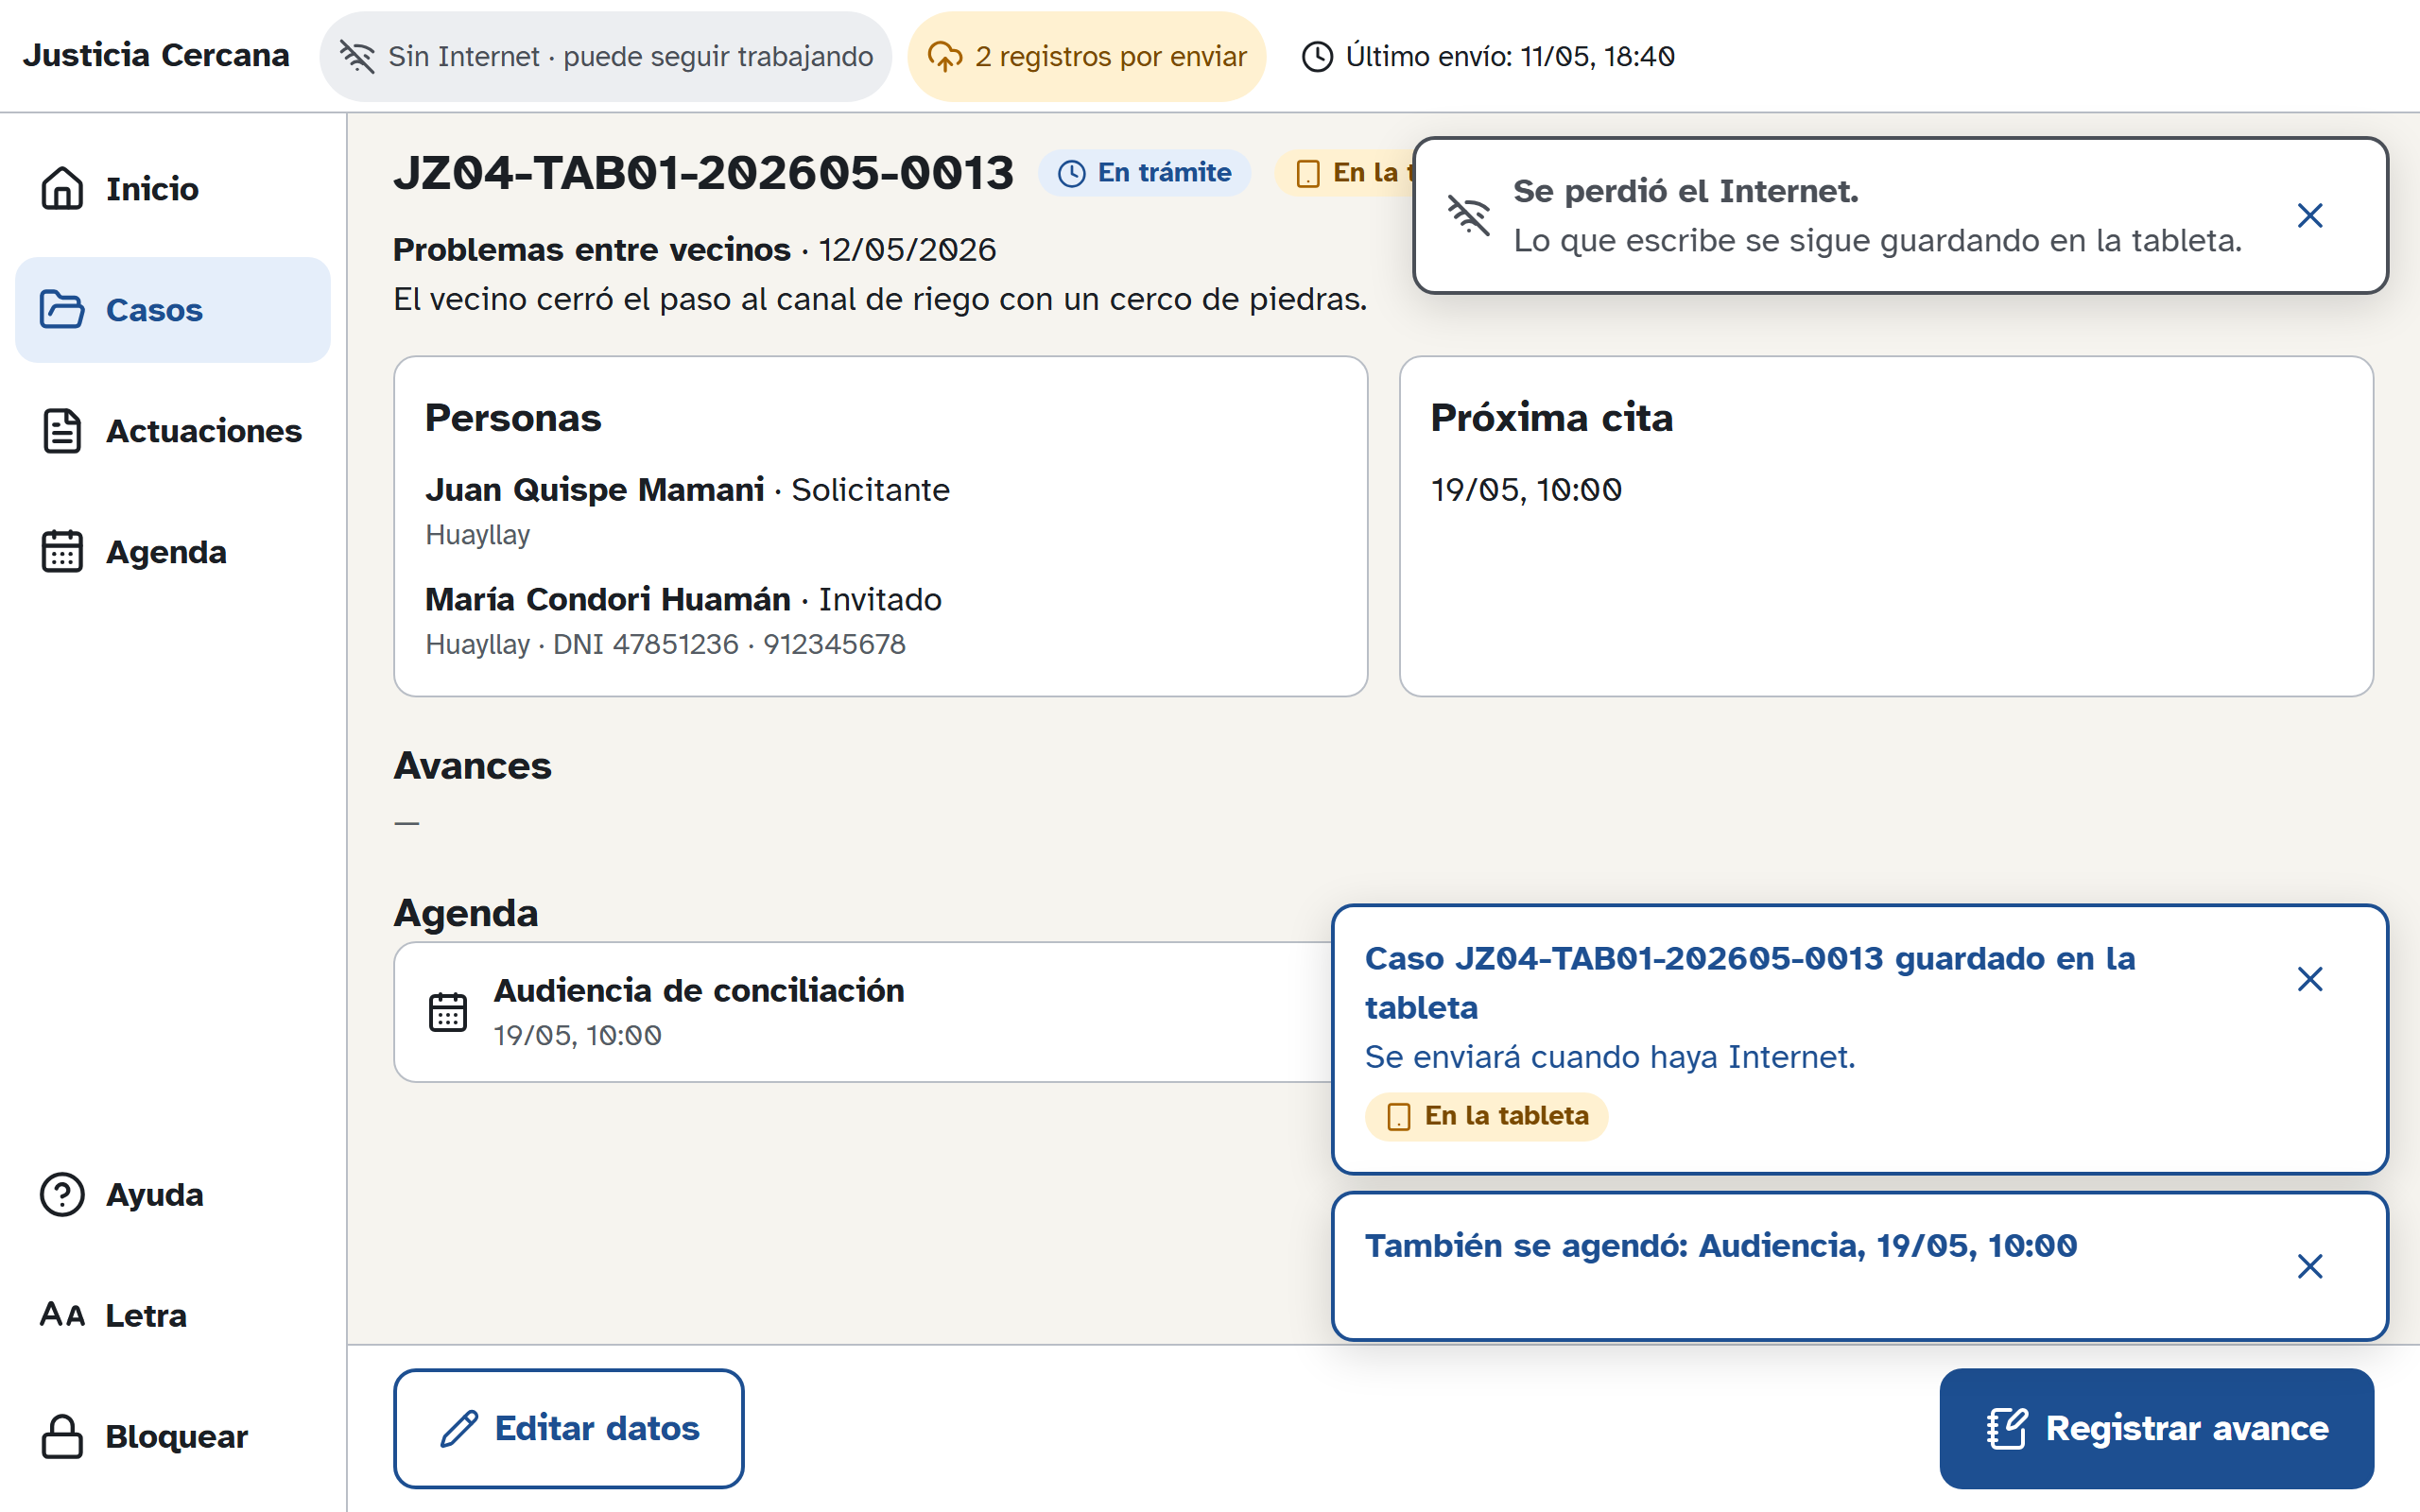
\includegraphics[width=\linewidth]{../../captures/F1-08_confirmacion-guardado.png}\\[-2pt]{\footnotesize\raggedright\textbf{P-04 · 8.} Confirmación ``guardado en la tableta'' + ``También se agendó'' y barra ``2 registros por enviar'' \emph{(Funcionamiento sin conexión)}\par}\end{minipage}\par\vspace{8pt}\noindent
\par\vspace{4pt}
\subsection*{Flujo 2}
\noindent
\begin{minipage}[t]{0.49\textwidth}\centering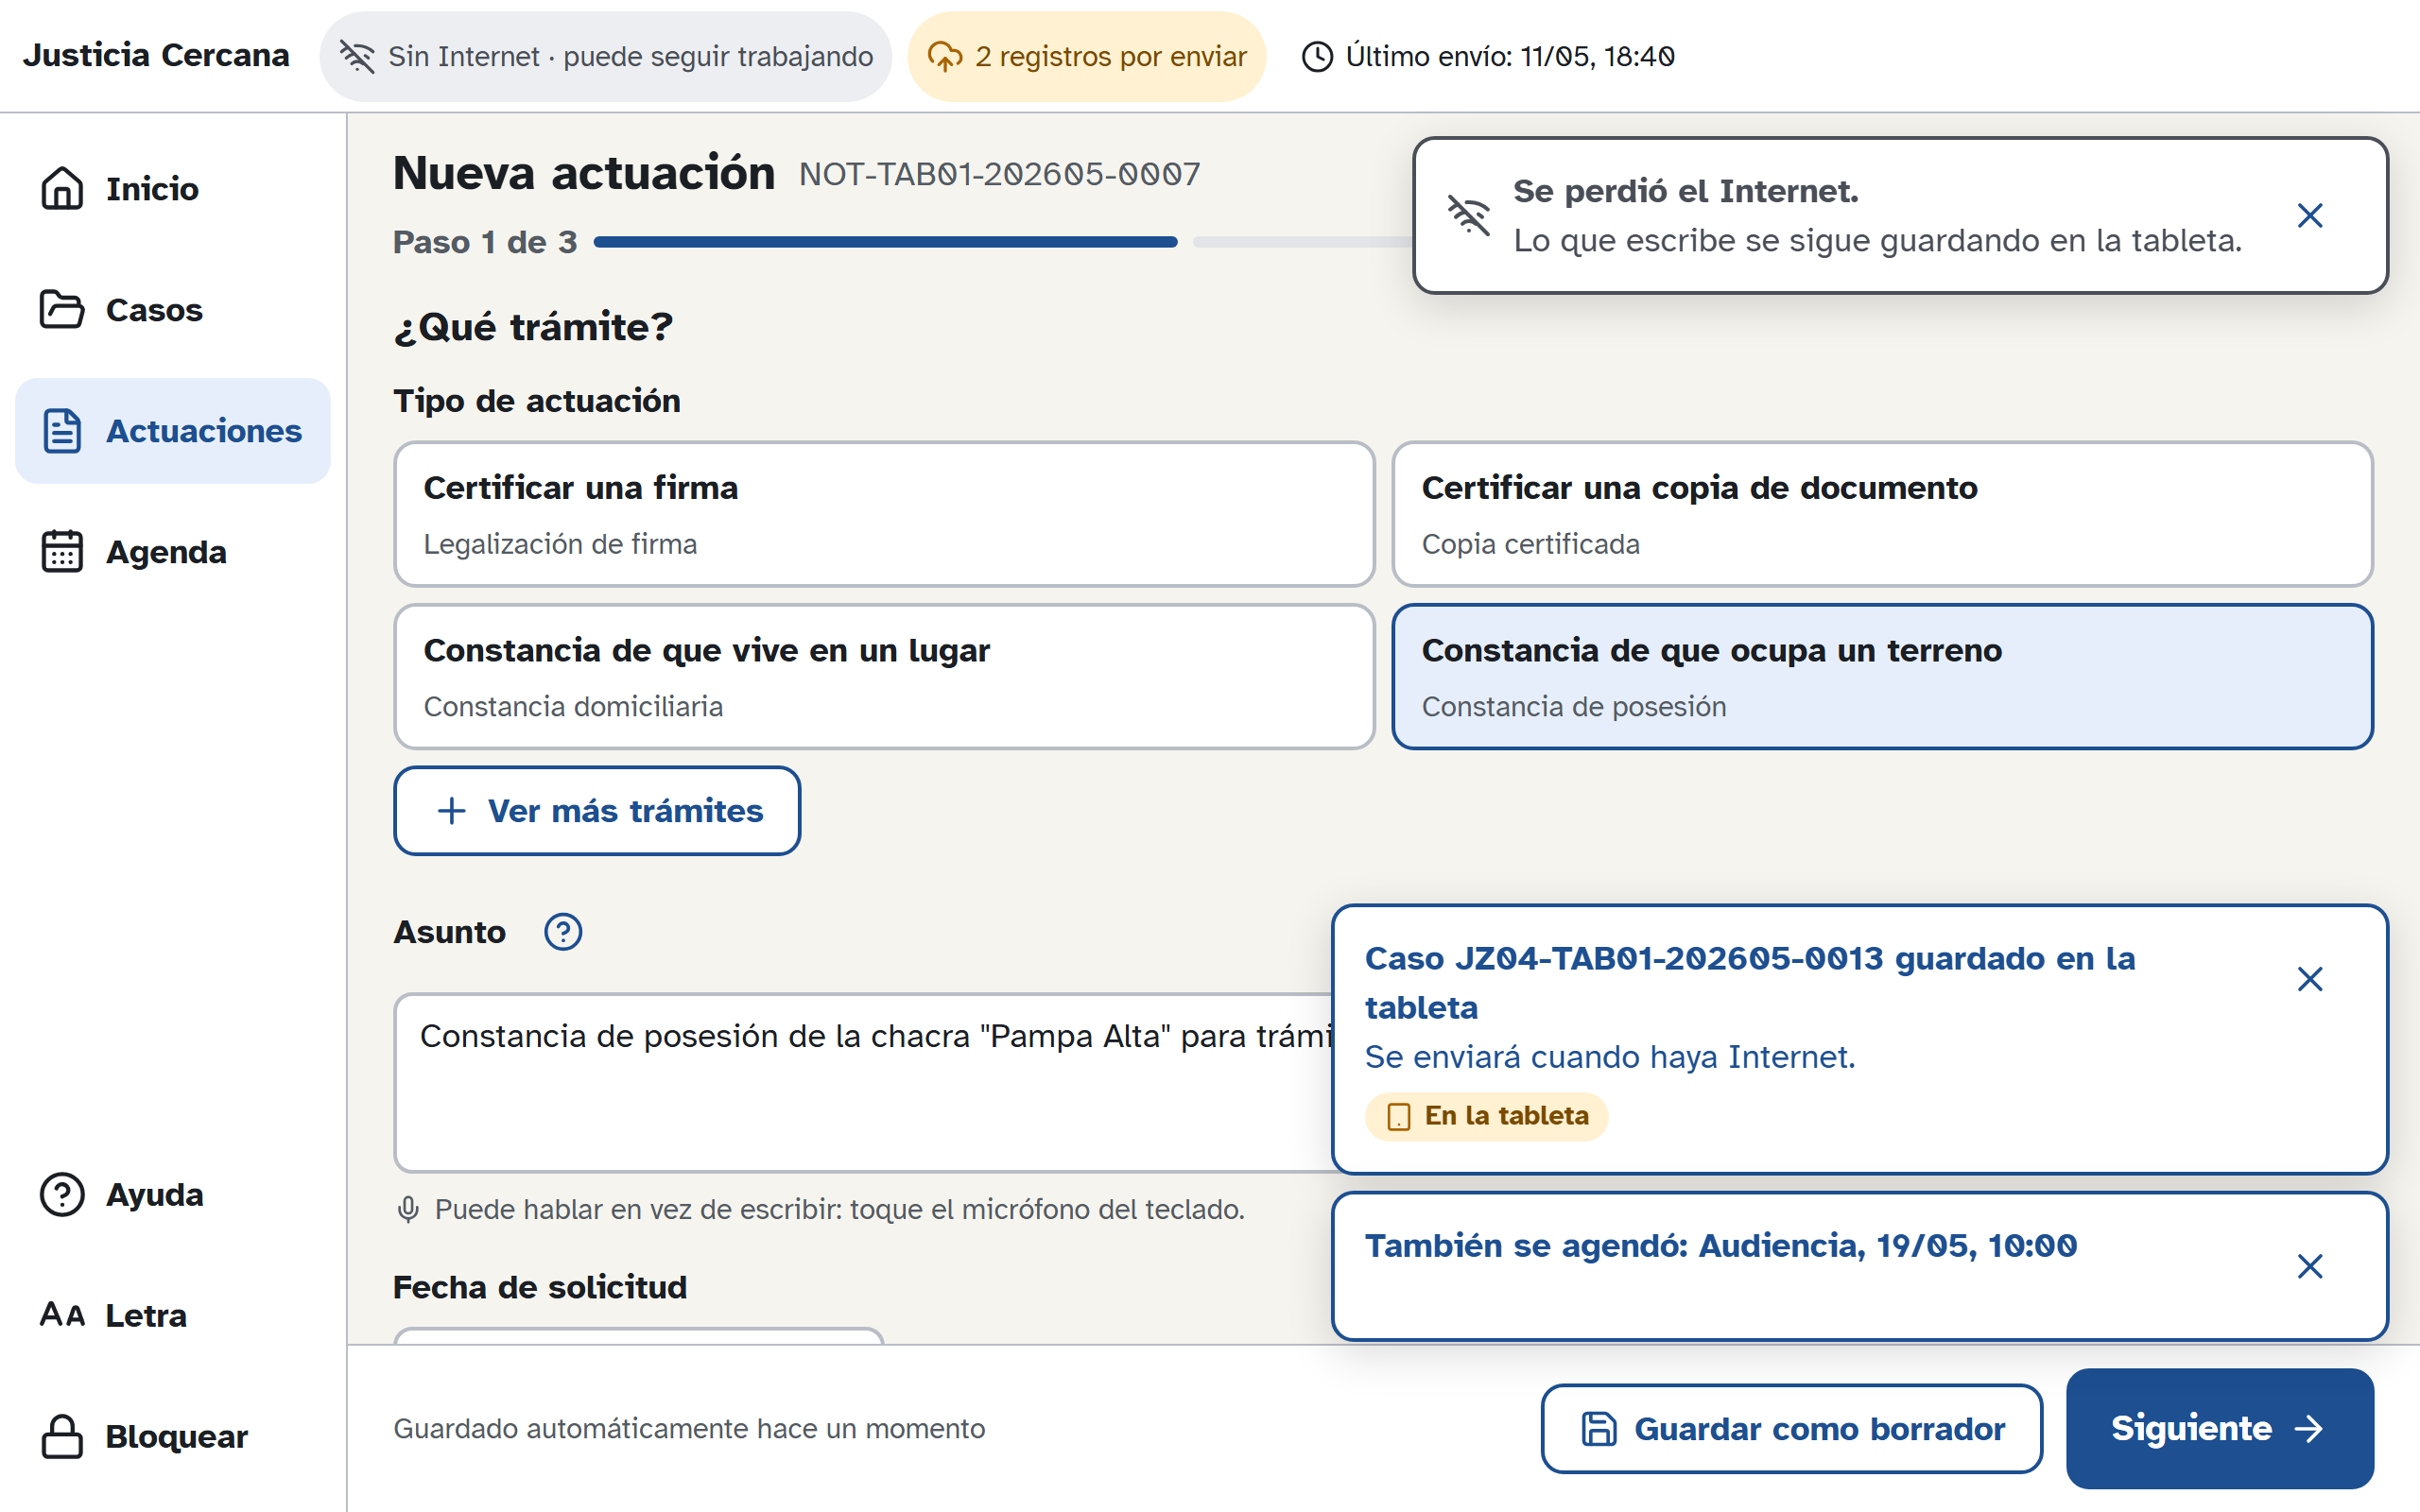
\includegraphics[width=\linewidth]{../../captures/F2-01_tipo-y-asunto.png}\\[-2pt]{\footnotesize\raggedright\textbf{P-06 · 1.} Tipo en lenguaje cotidiano (4 tarjetas + Ver más) y asunto \emph{(Cobertura y funcionamiento de los módulos)}\par}\end{minipage}\hfill
\begin{minipage}[t]{0.49\textwidth}\centering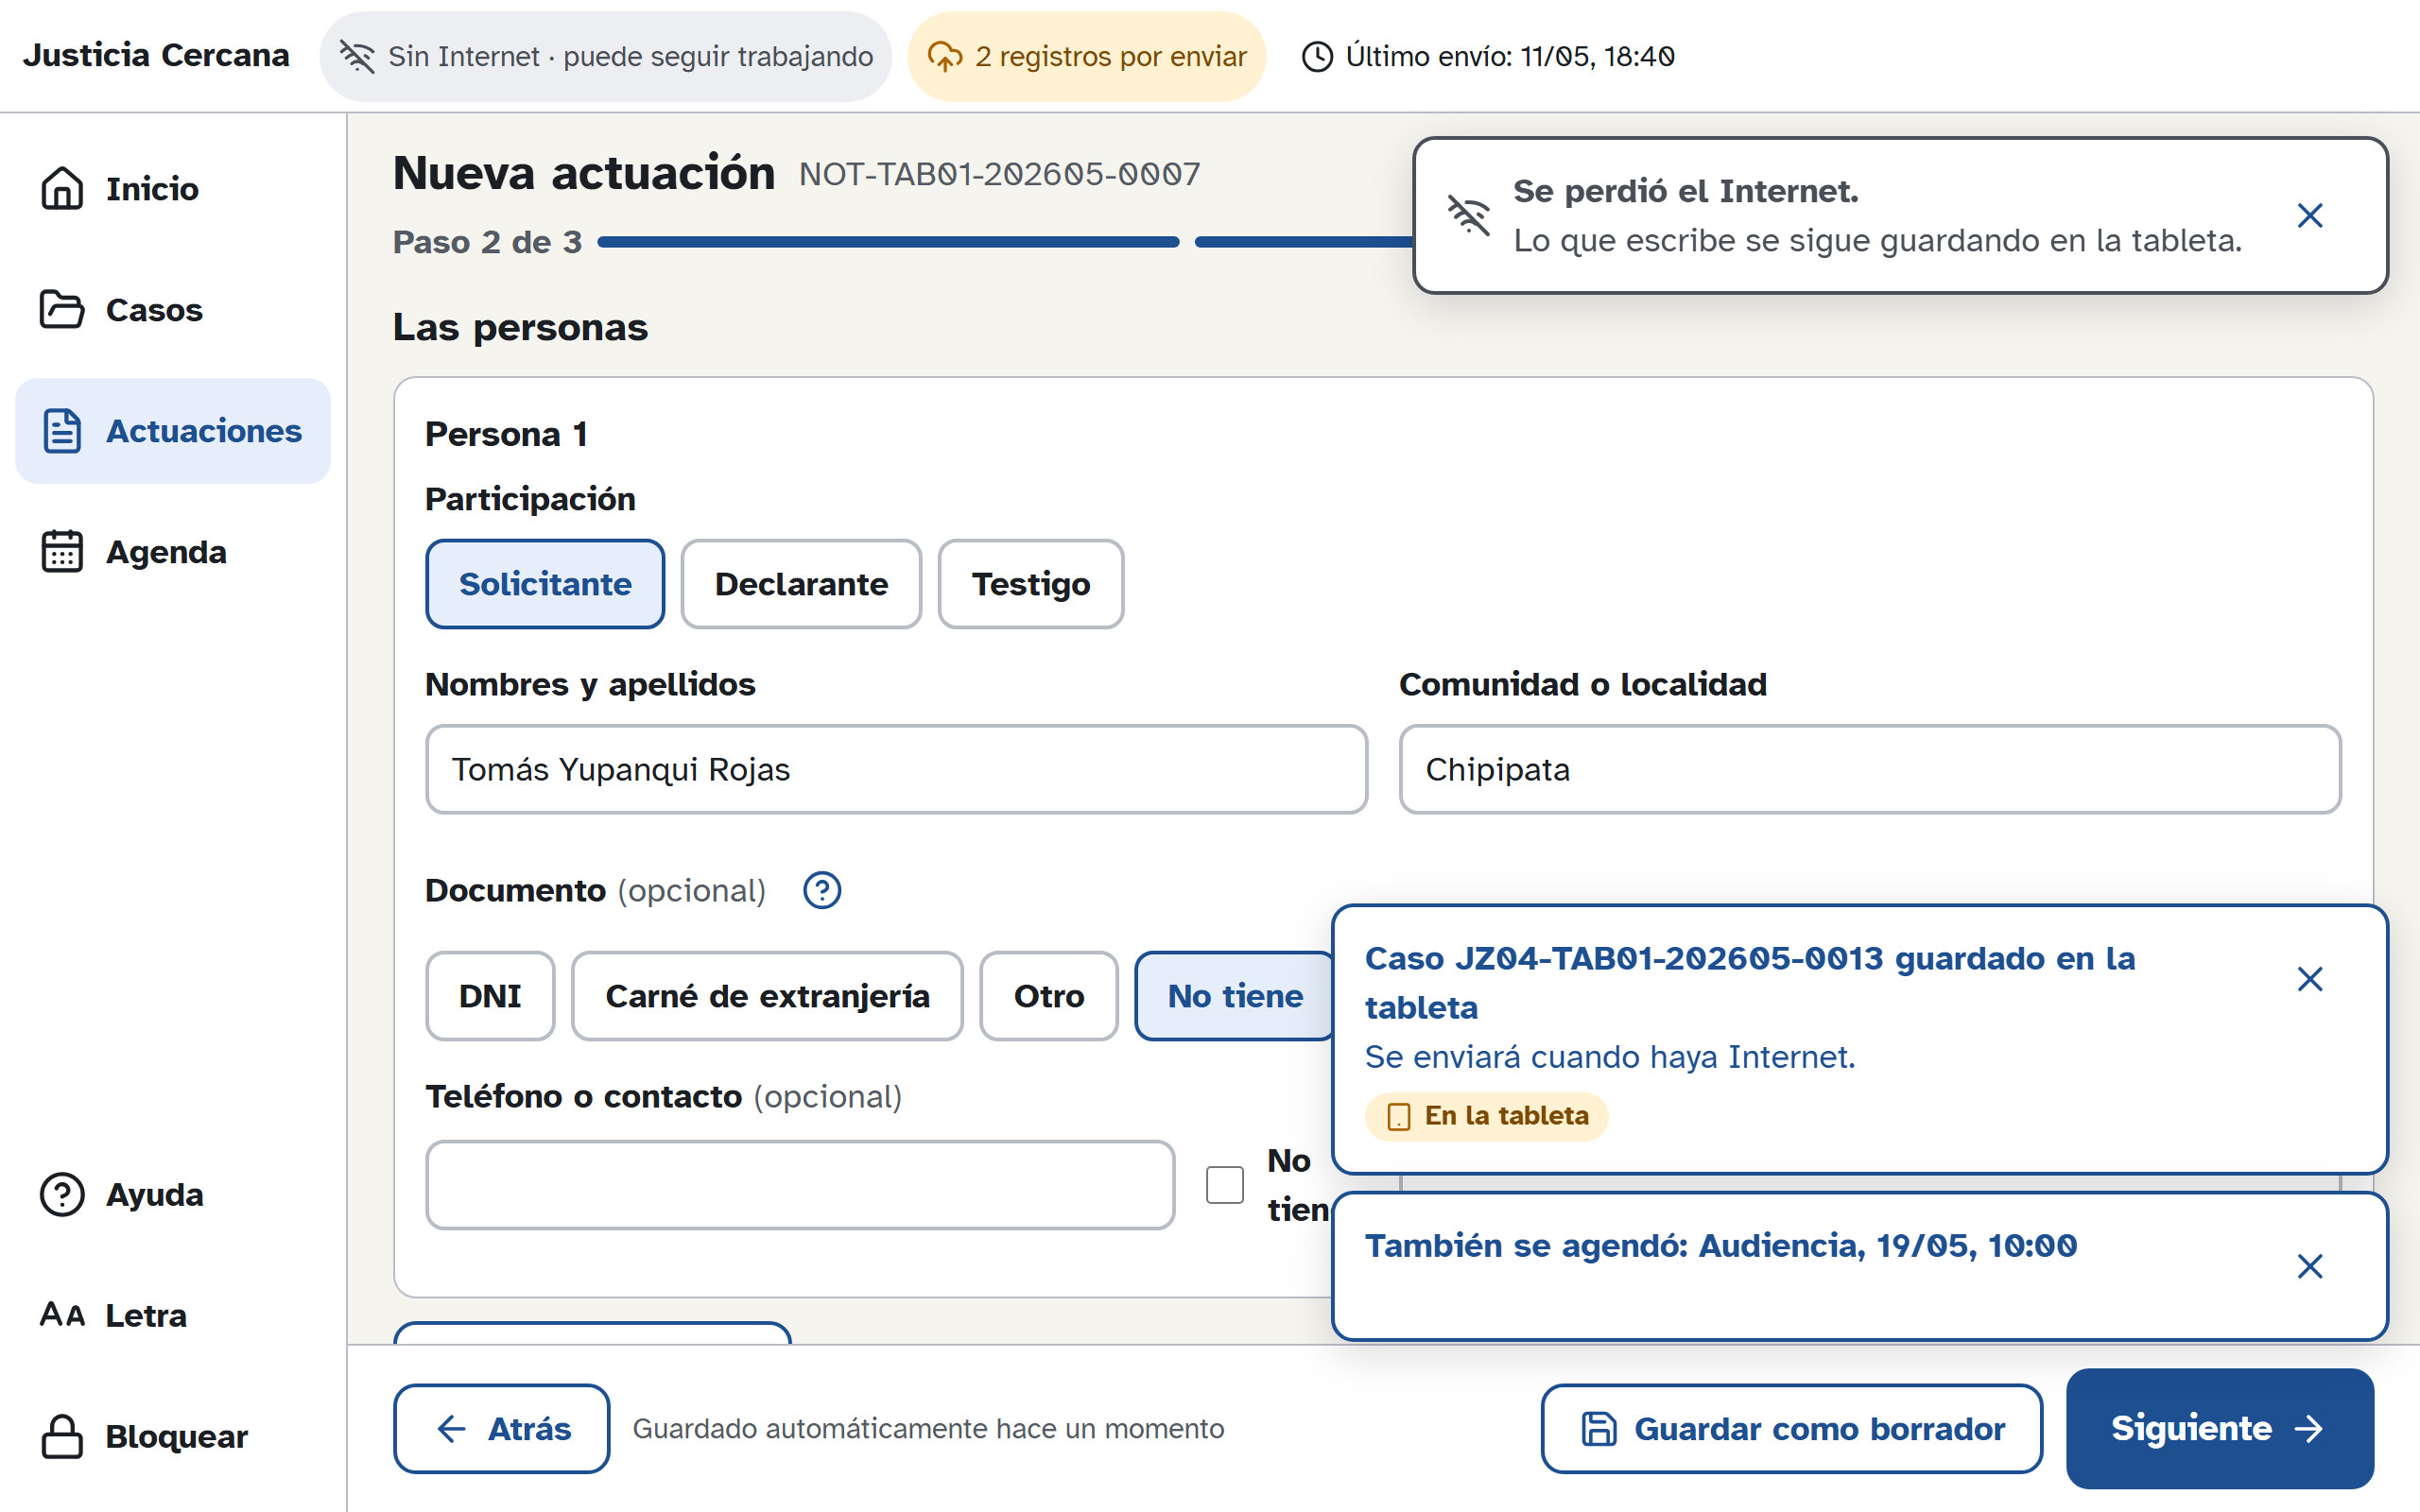
\includegraphics[width=\linewidth]{../../captures/F2-02_solicitante.png}\\[-2pt]{\footnotesize\raggedright\textbf{P-06 · 2.} Solicitante agregado sin duplicados; guardado automático \emph{(Cobertura y funcionamiento de los módulos)}\par}\end{minipage}\par\vspace{8pt}\noindent
\begin{minipage}[t]{0.49\textwidth}\centering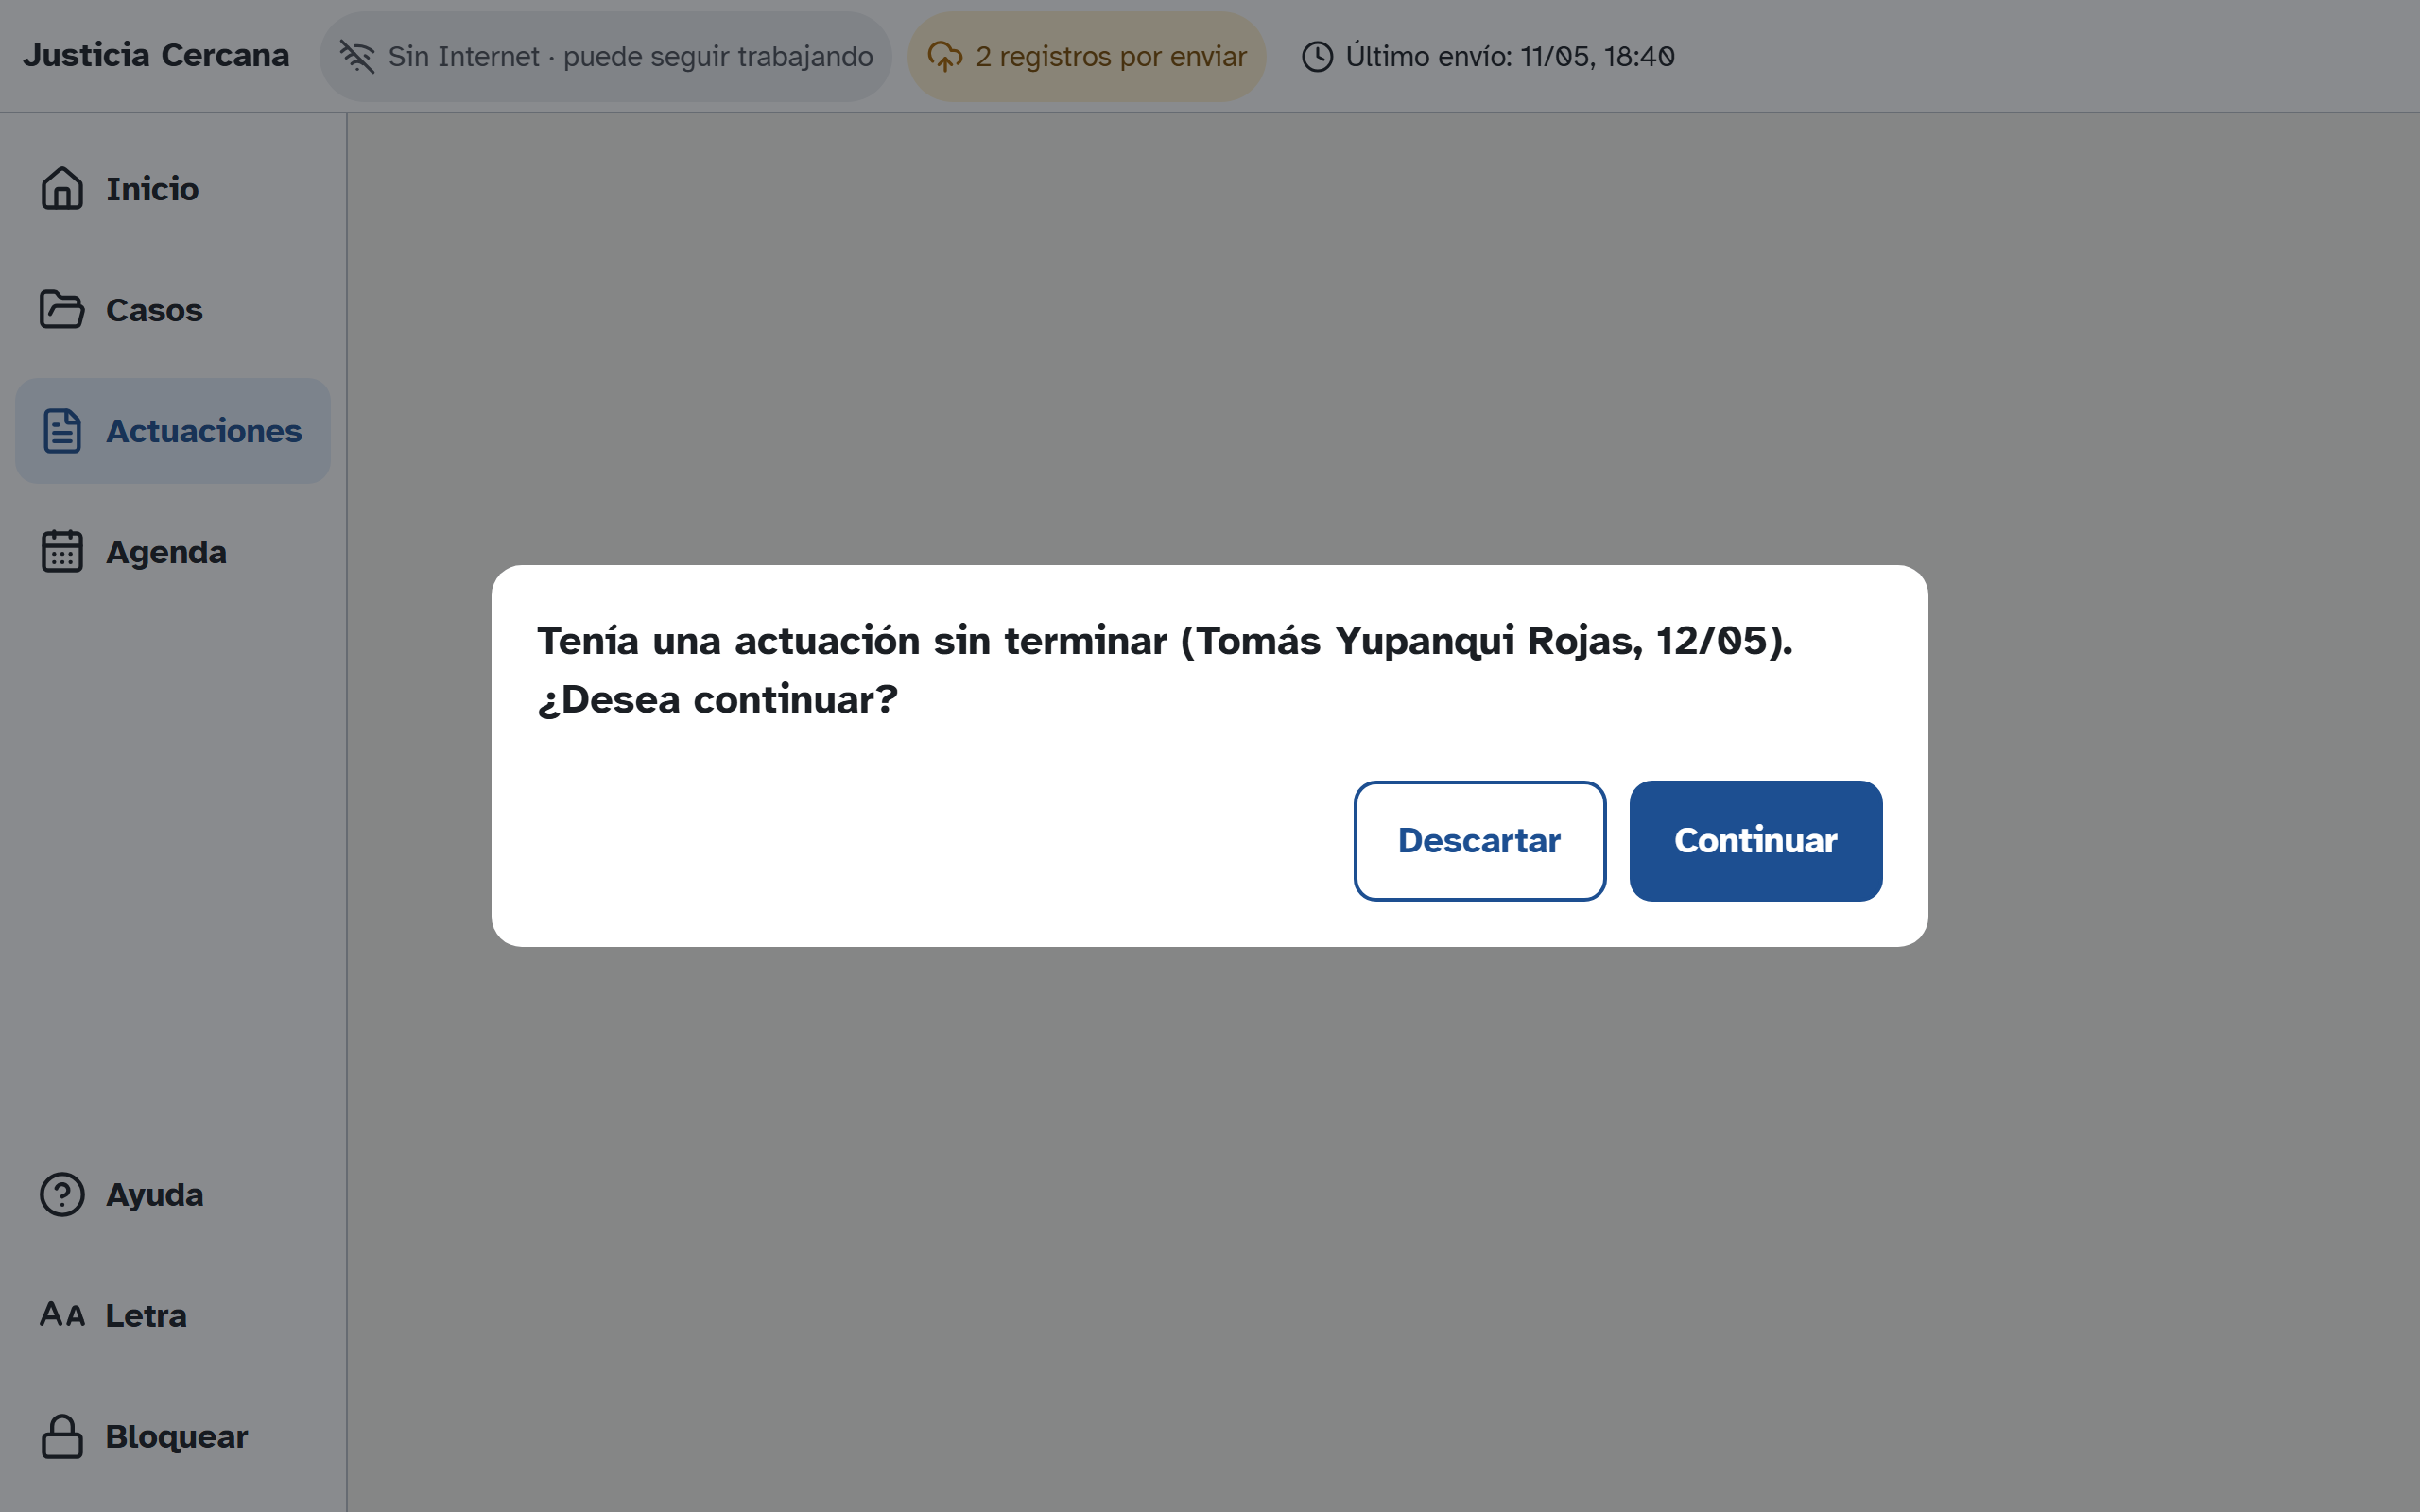
\includegraphics[width=\linewidth]{../../captures/F2-03a_recuperacion.png}\\[-2pt]{\footnotesize\raggedright\textbf{P-06 · 3.} Recuperación tras cierre inesperado: ``Tenía una actuación sin terminar. ¿Desea continuar?'' \emph{(Funcionamiento sin conexión)}\par}\end{minipage}\hfill
\begin{minipage}[t]{0.49\textwidth}\centering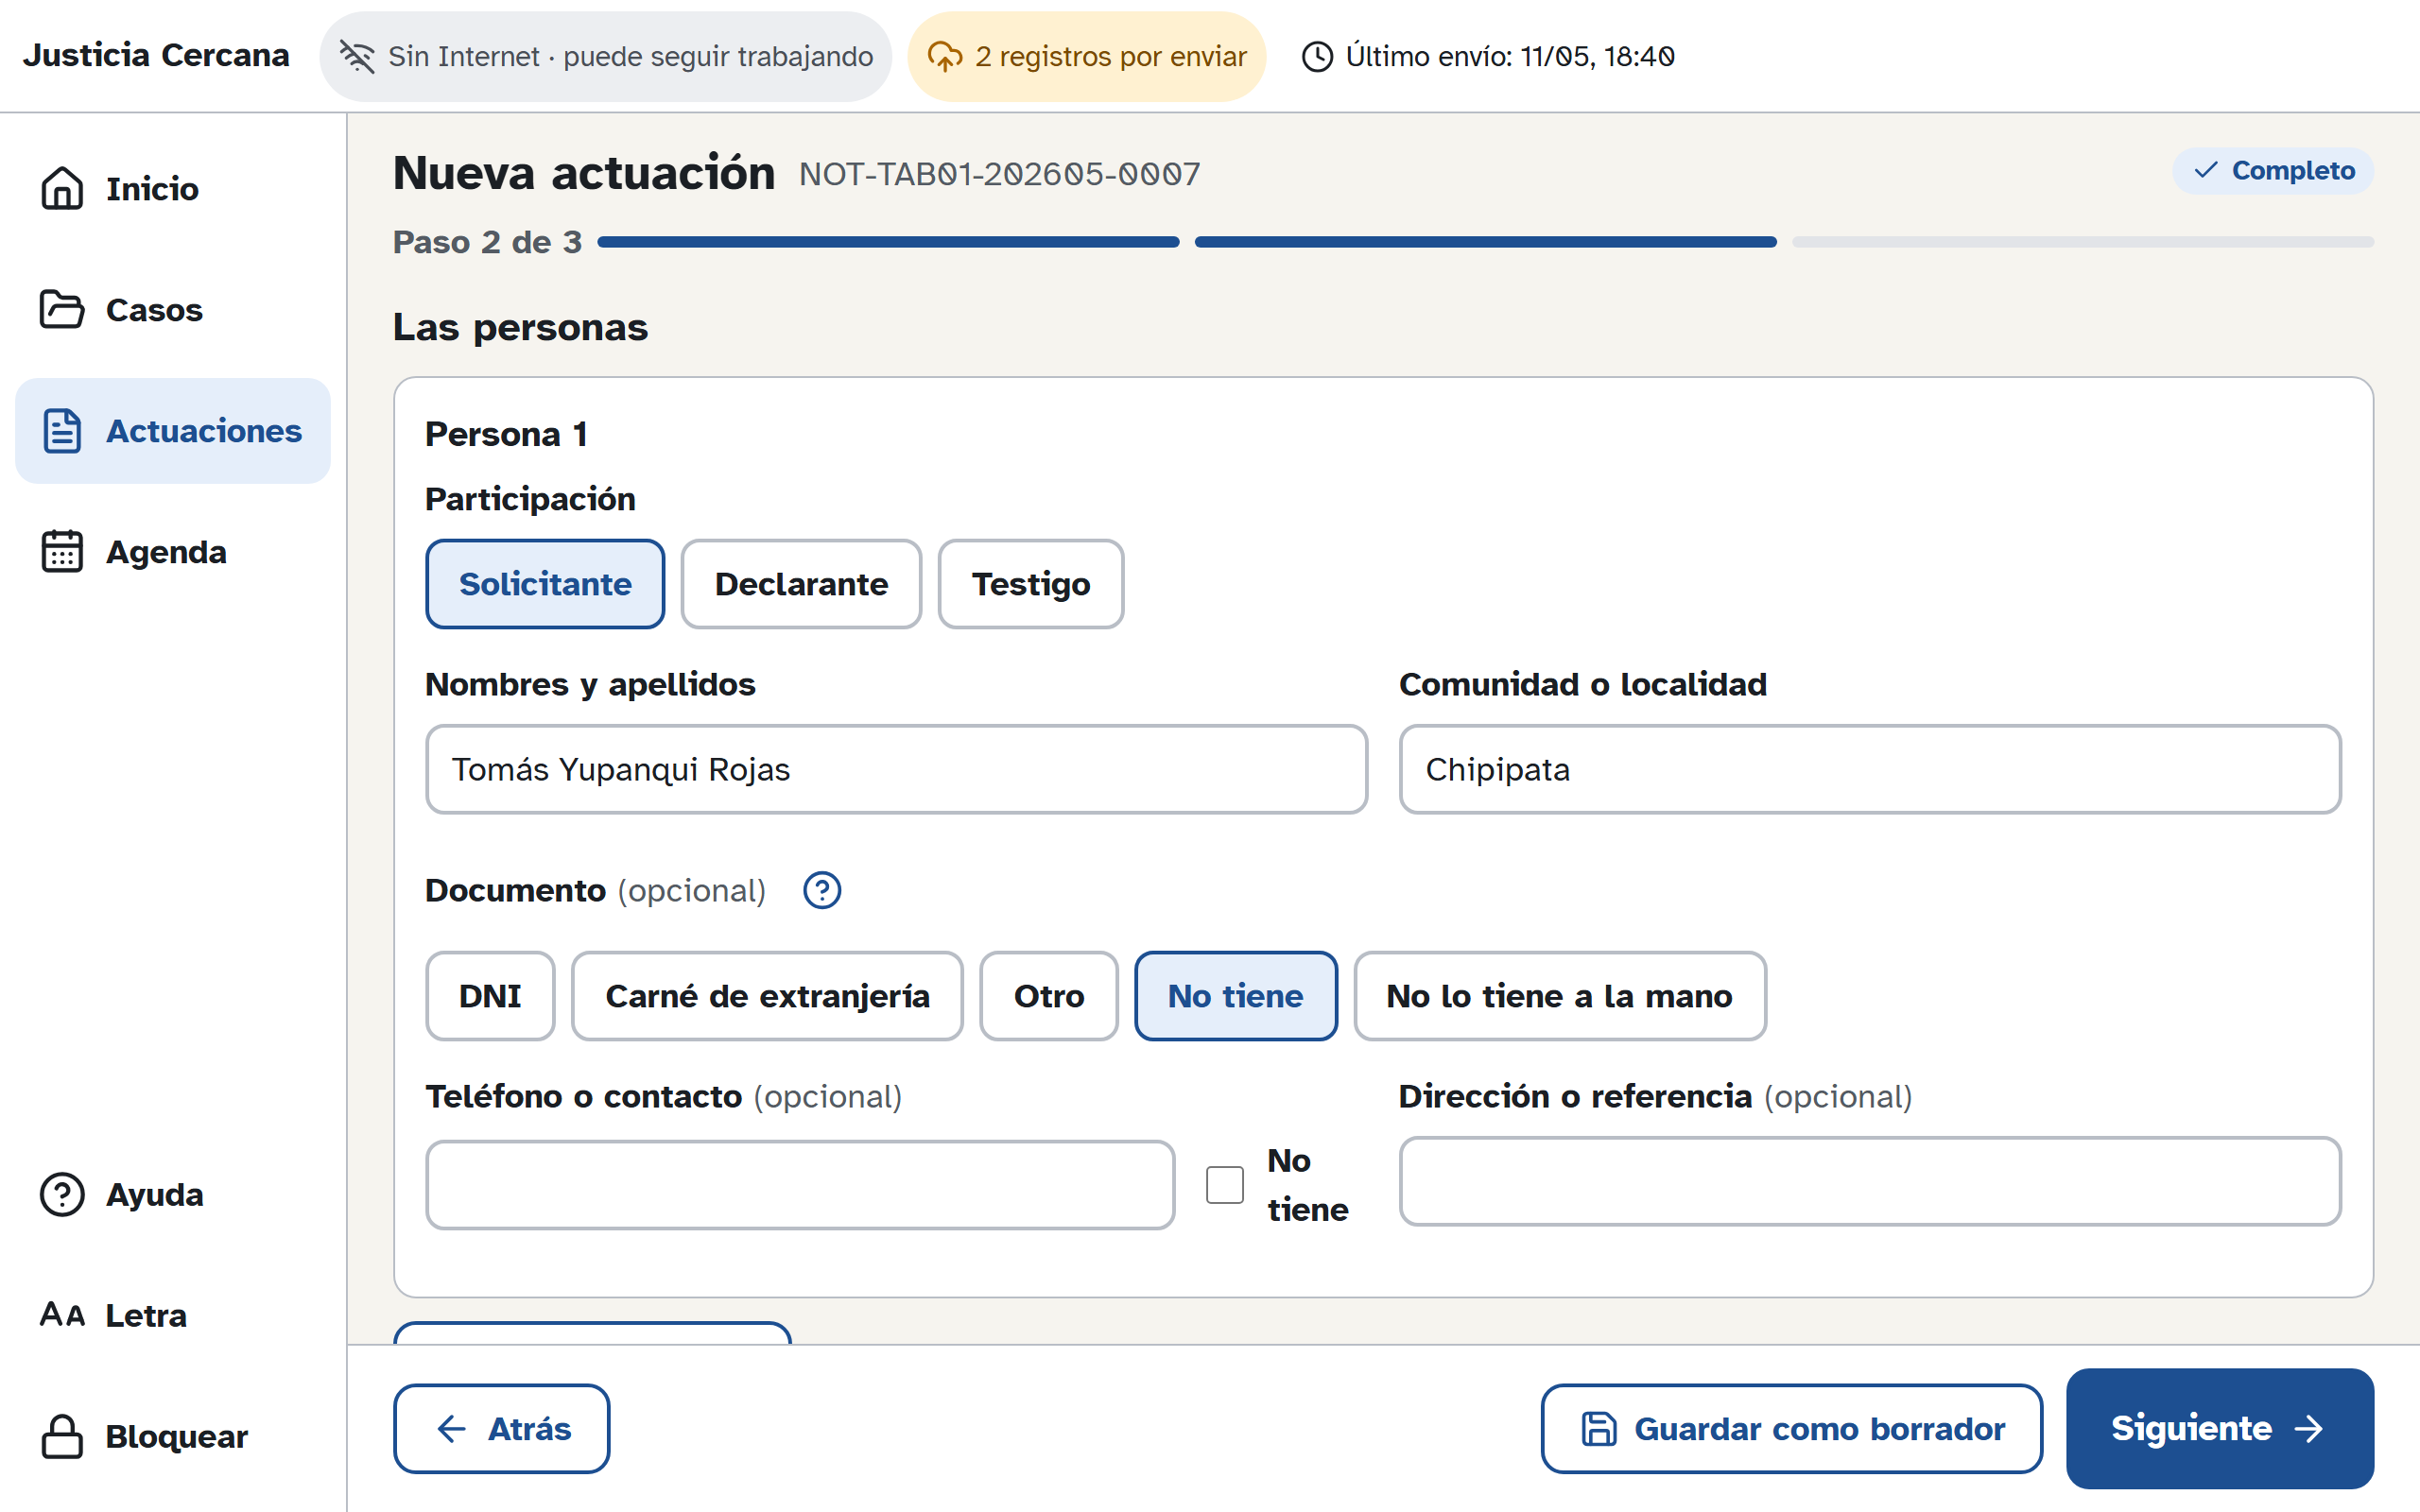
\includegraphics[width=\linewidth]{../../captures/F2-03b_continua-paso2.png}\\[-2pt]{\footnotesize\raggedright\textbf{P-06 · 3.} Continúa en el mismo paso con los datos recuperados \emph{(Funcionamiento sin conexión)}\par}\end{minipage}\par\vspace{8pt}\noindent
\begin{minipage}[t]{0.49\textwidth}\centering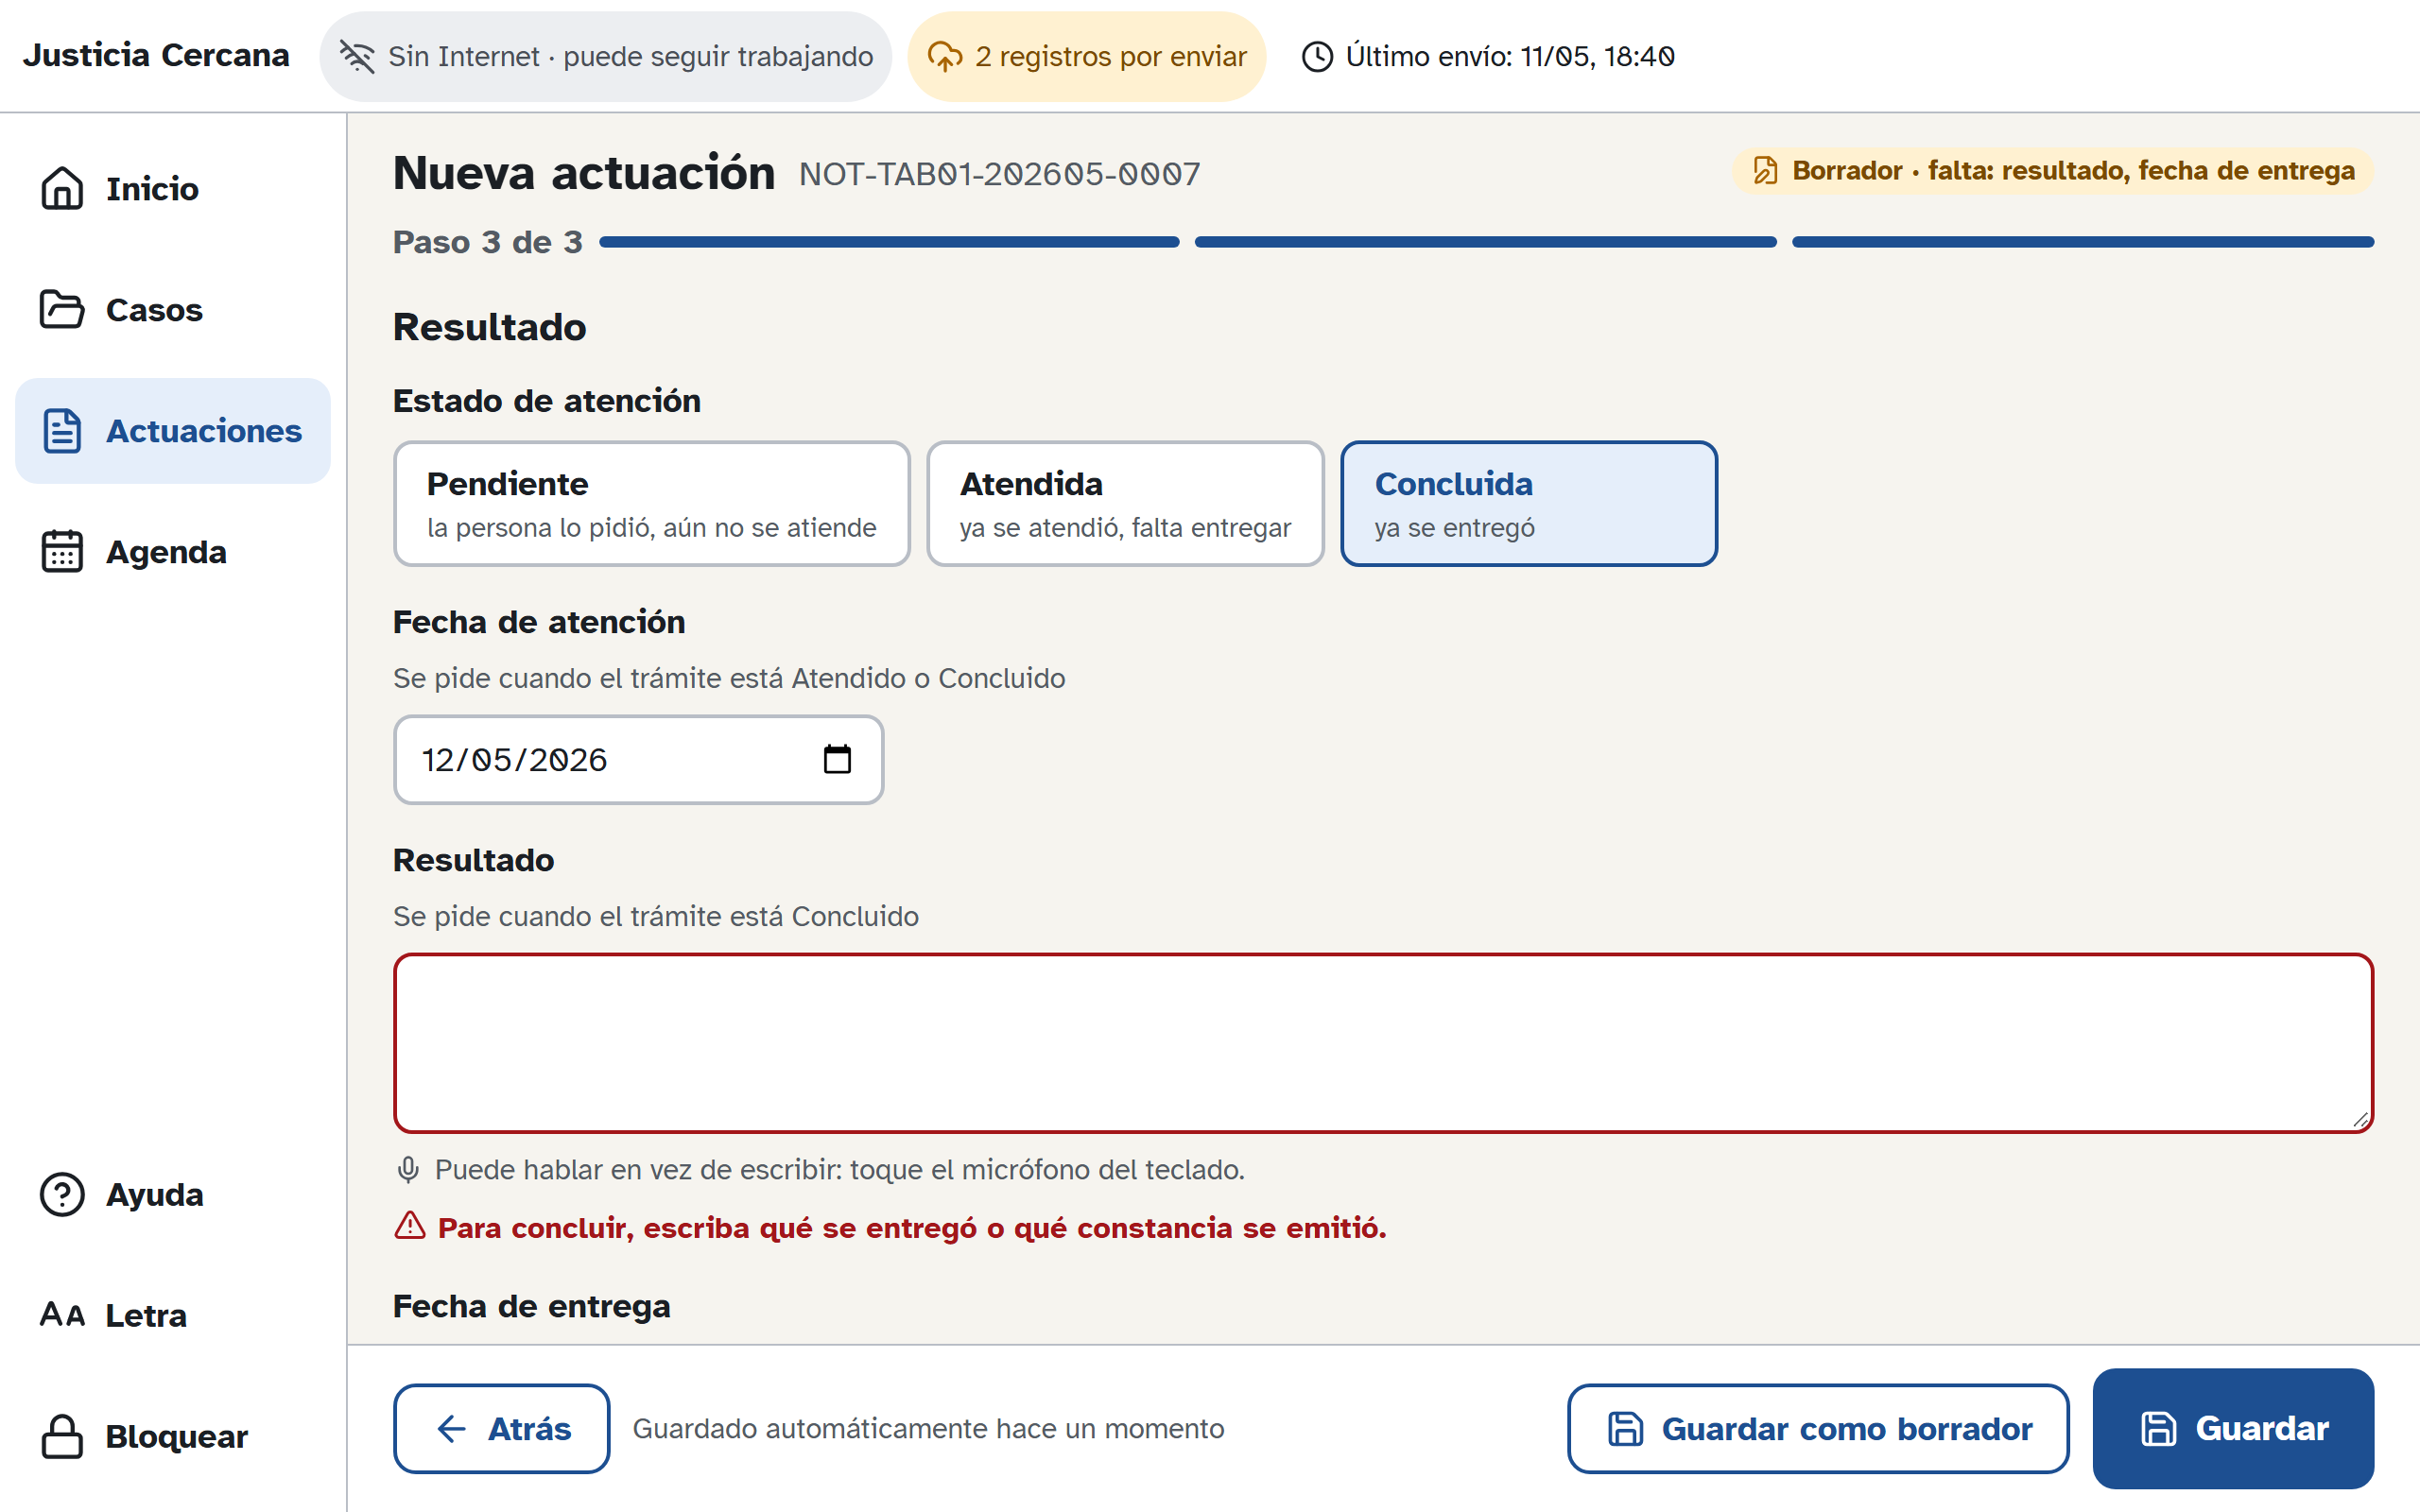
\includegraphics[width=\linewidth]{../../captures/F2-04_error-concluida-sin-resultado.png}\\[-2pt]{\footnotesize\raggedright\textbf{P-06 · 4.} Condicional: Concluida sin resultado $\rightarrow$ mensaje; líneas ``Se pide cuando…''; Borrador \emph{(Principios de diseño y heurísticas)}\par}\end{minipage}\hfill
\begin{minipage}[t]{0.49\textwidth}\centering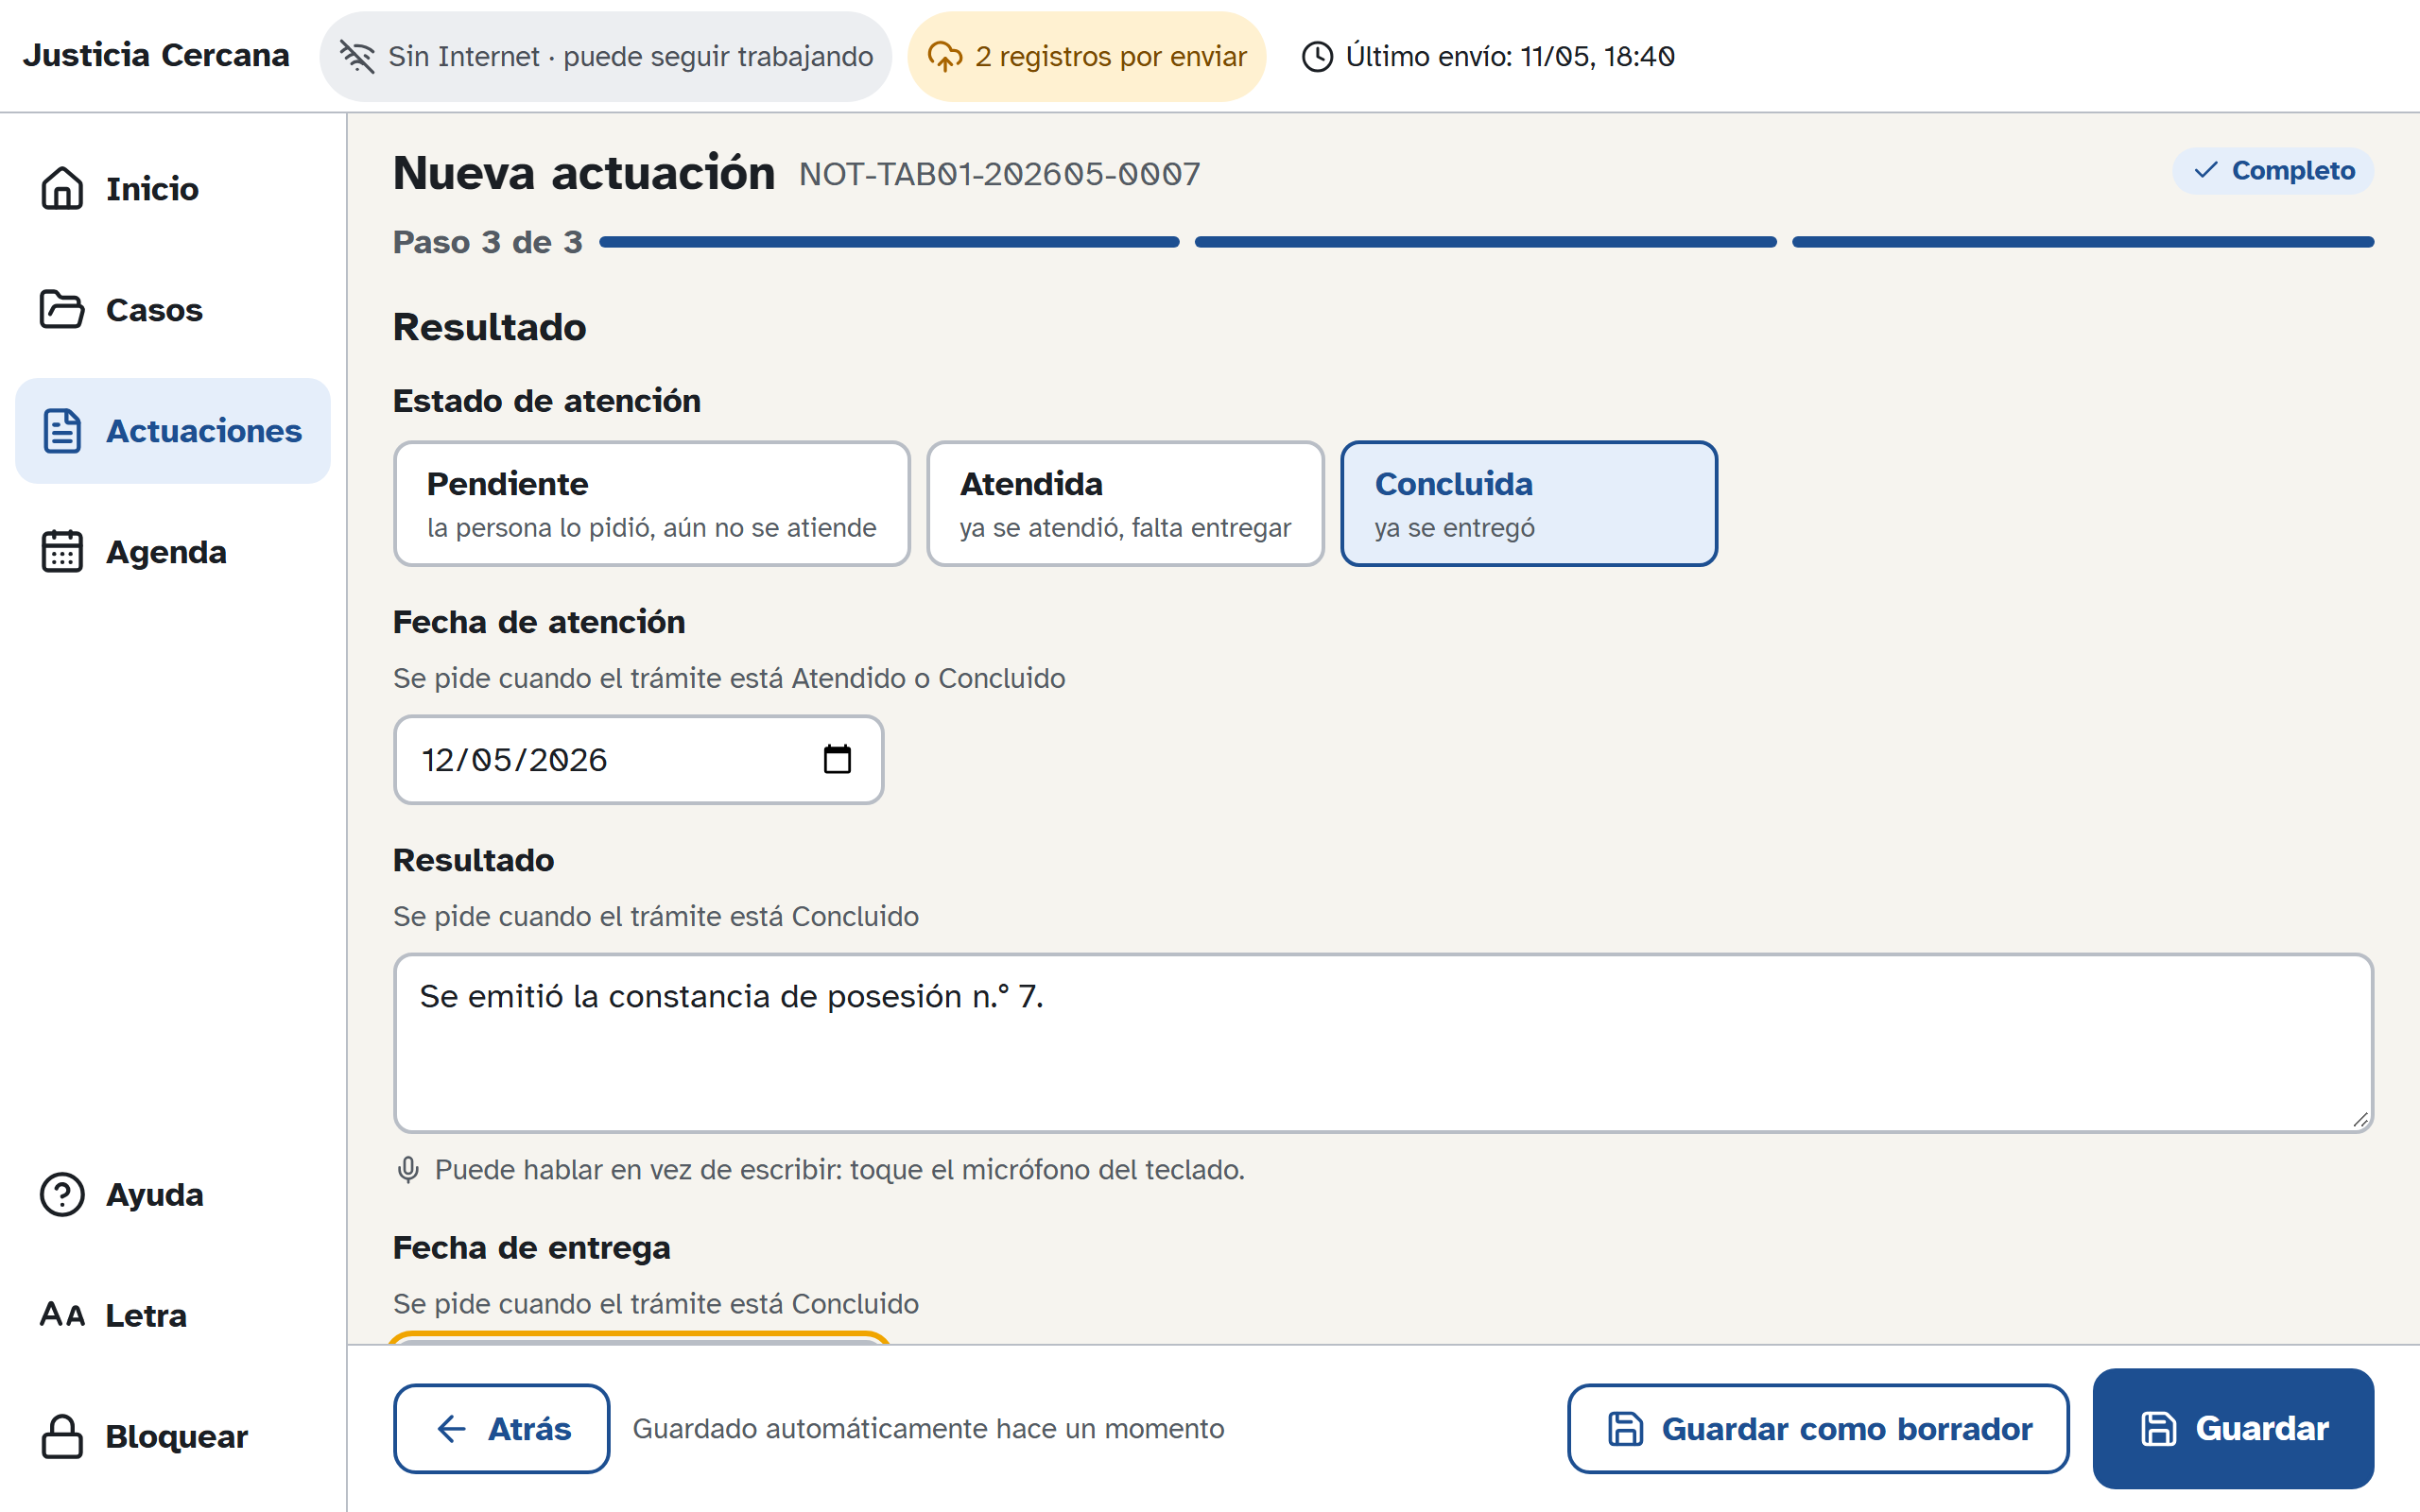
\includegraphics[width=\linewidth]{../../captures/F2-05_completo.png}\\[-2pt]{\footnotesize\raggedright\textbf{P-06 · 5.} Resultado y fecha de entrega $\rightarrow$ el registro pasa de Borrador a Completo \emph{(Cobertura y funcionamiento de los módulos)}\par}\end{minipage}\par\vspace{8pt}\noindent
\begin{minipage}[t]{0.49\textwidth}\centering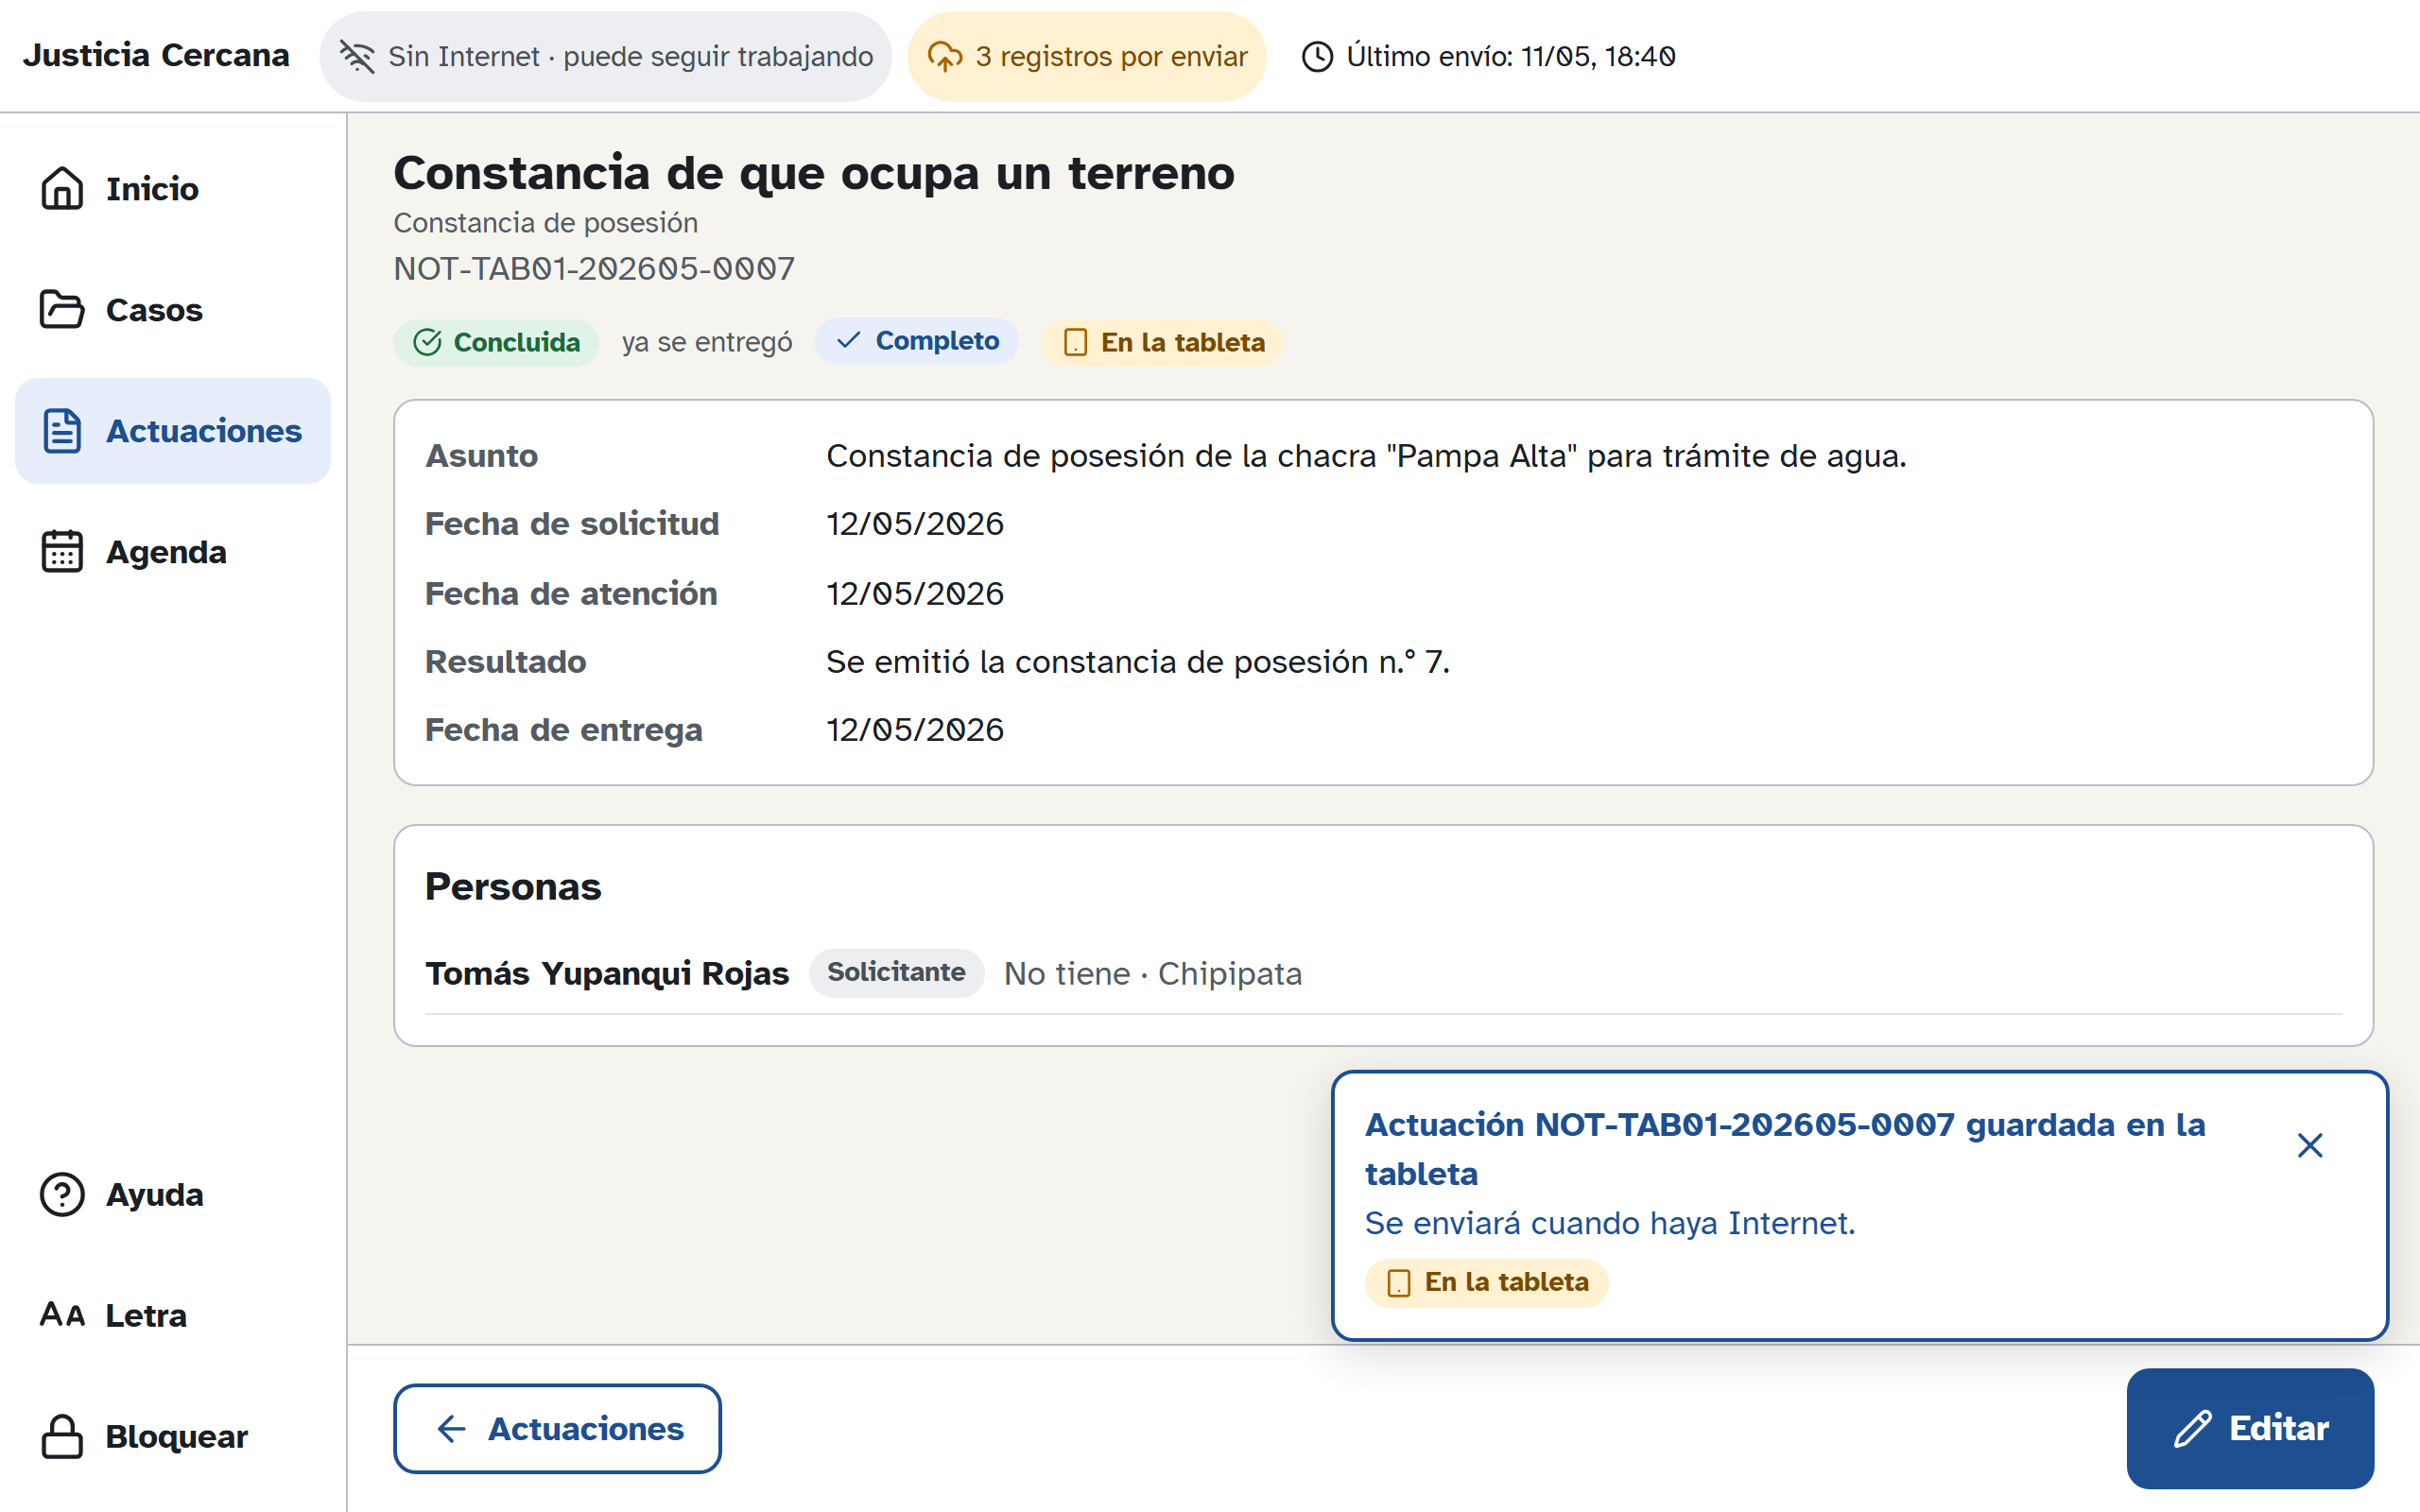
\includegraphics[width=\linewidth]{../../captures/F2-06_confirmacion-guardado.png}\\[-2pt]{\footnotesize\raggedright\textbf{P-06 · 6.} Confirmación en la tableta; barra ``3 registros por enviar'' \emph{(Funcionamiento sin conexión)}\par}\end{minipage}\hfill
\par\vspace{4pt}
\subsection*{Flujo 3}
\noindent
\begin{minipage}[t]{0.49\textwidth}\centering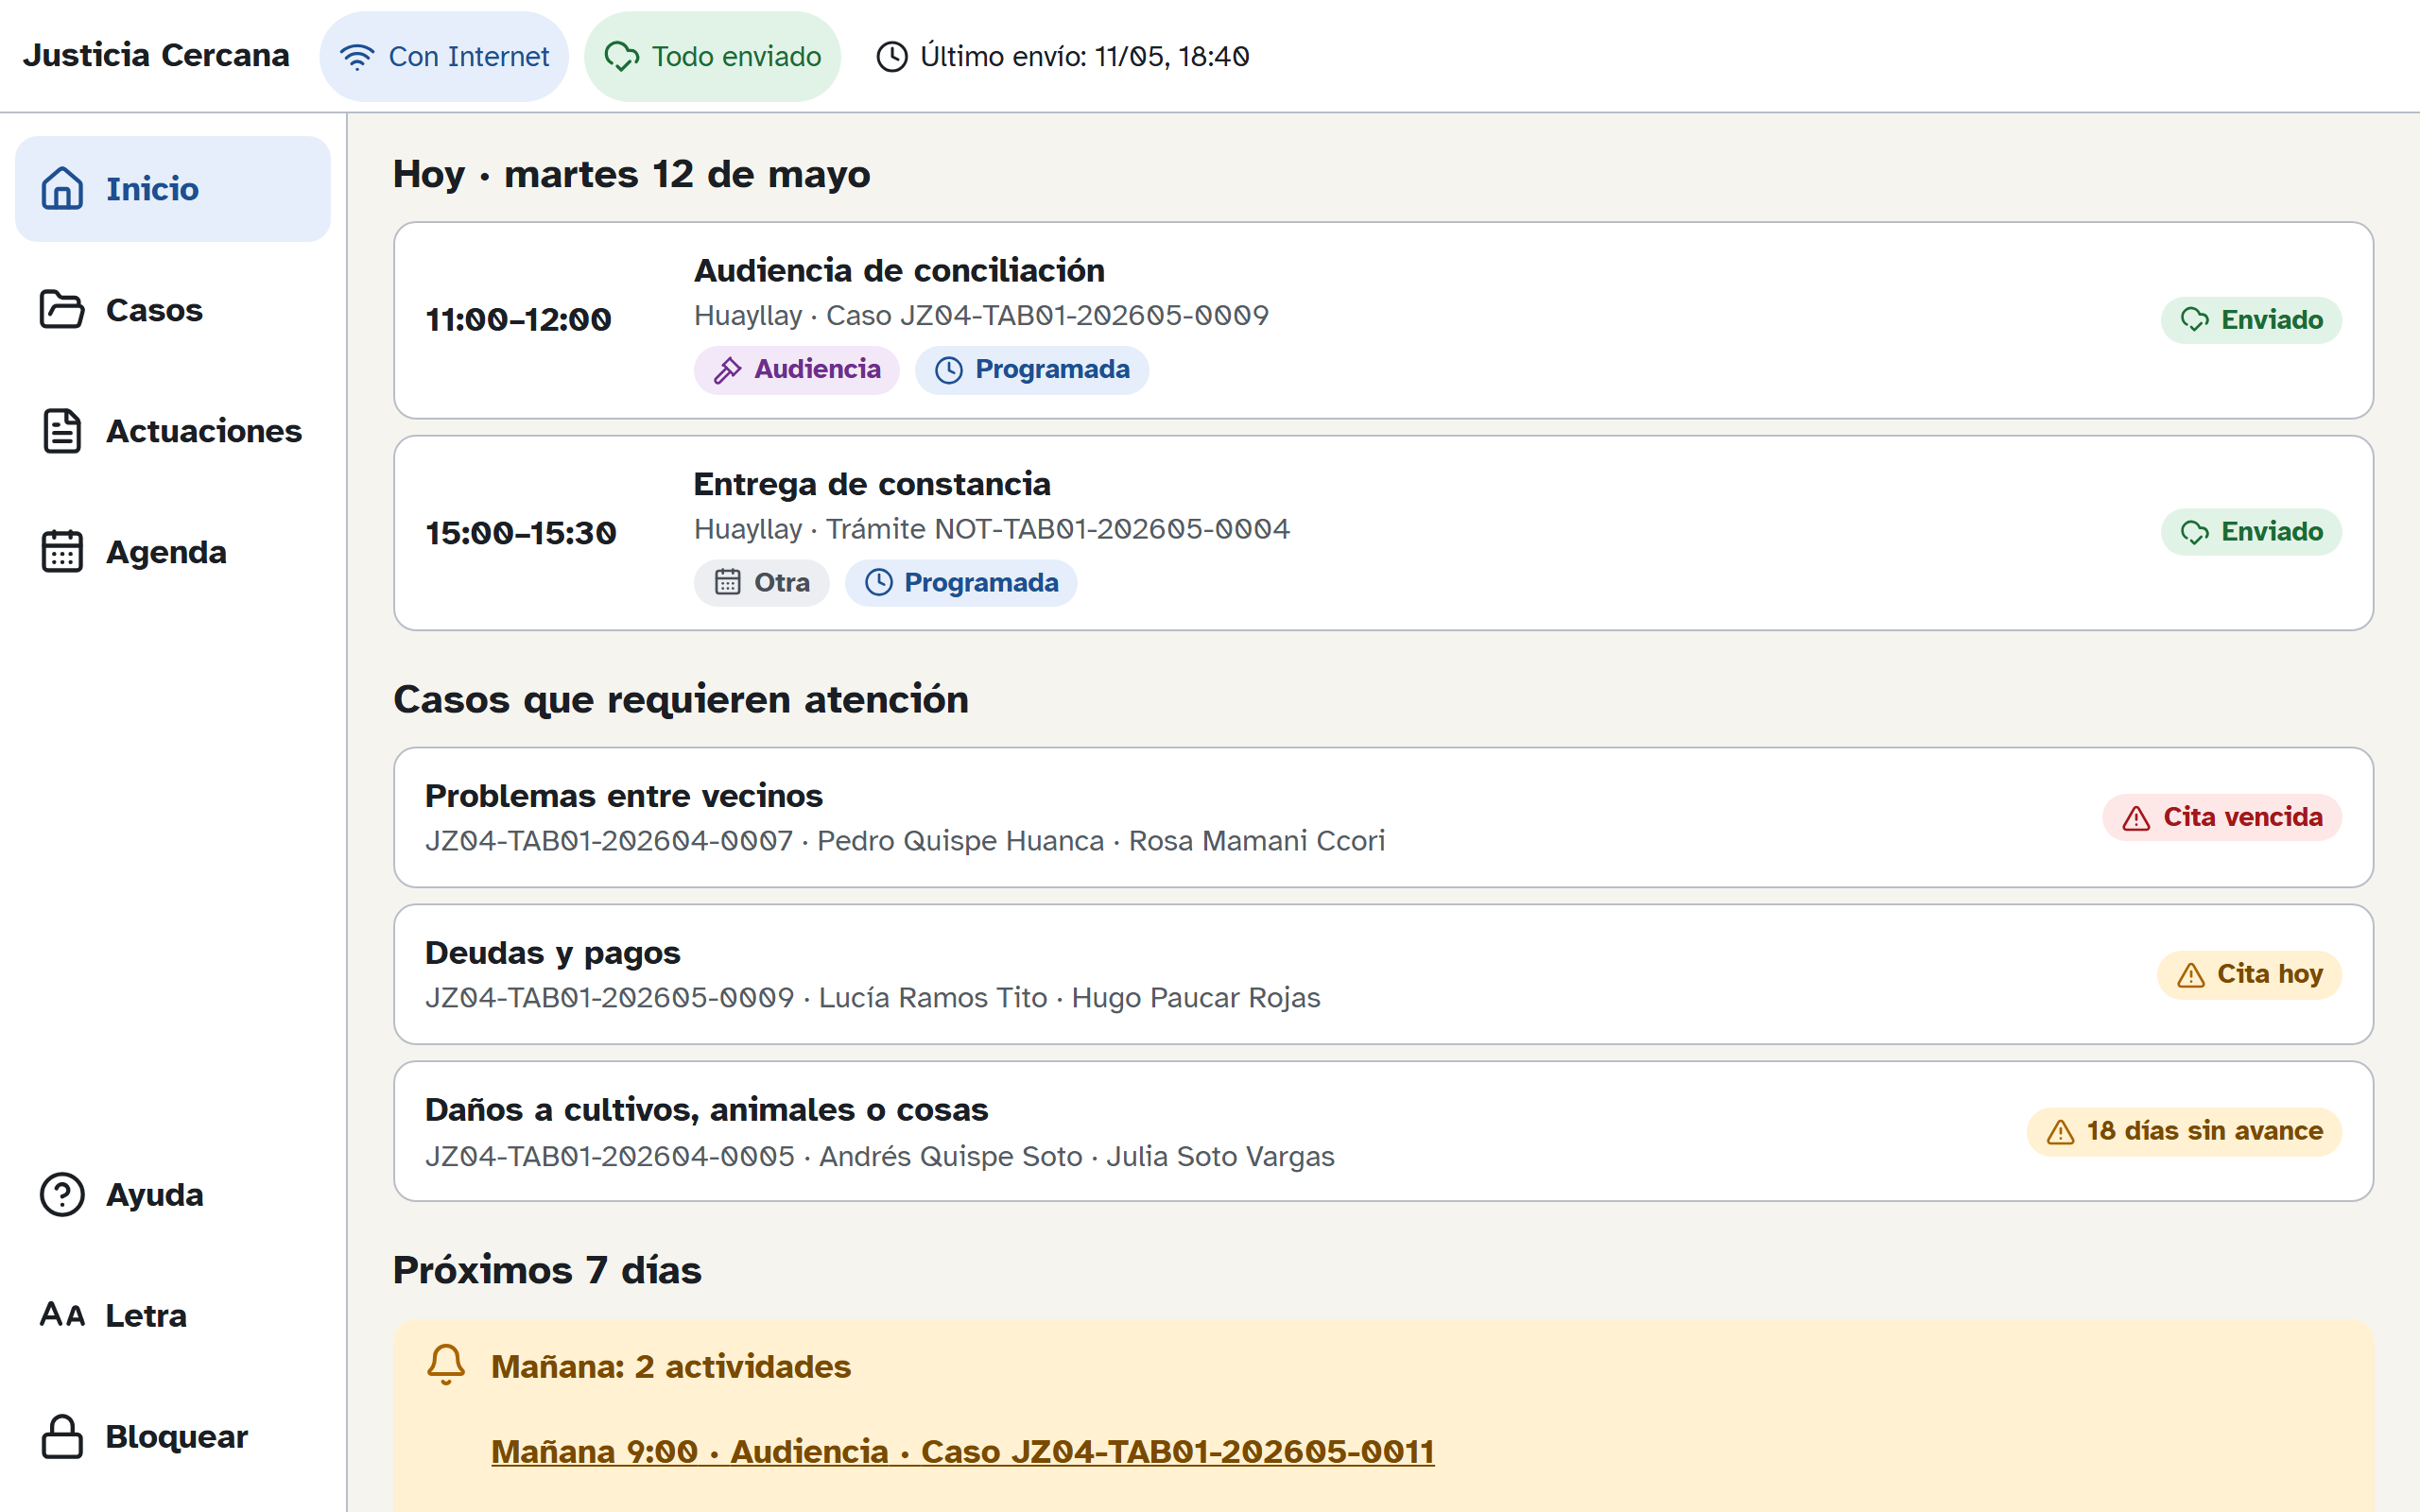
\includegraphics[width=\linewidth]{../../captures/F3-01_inicio-manana.png}\\[-2pt]{\footnotesize\raggedright\textbf{P-01 · 1.} Aviso de próximas ``Mañana: 2 actividades'' en Inicio \emph{(Cobertura y funcionamiento de los módulos)}\par}\end{minipage}\hfill
\begin{minipage}[t]{0.49\textwidth}\centering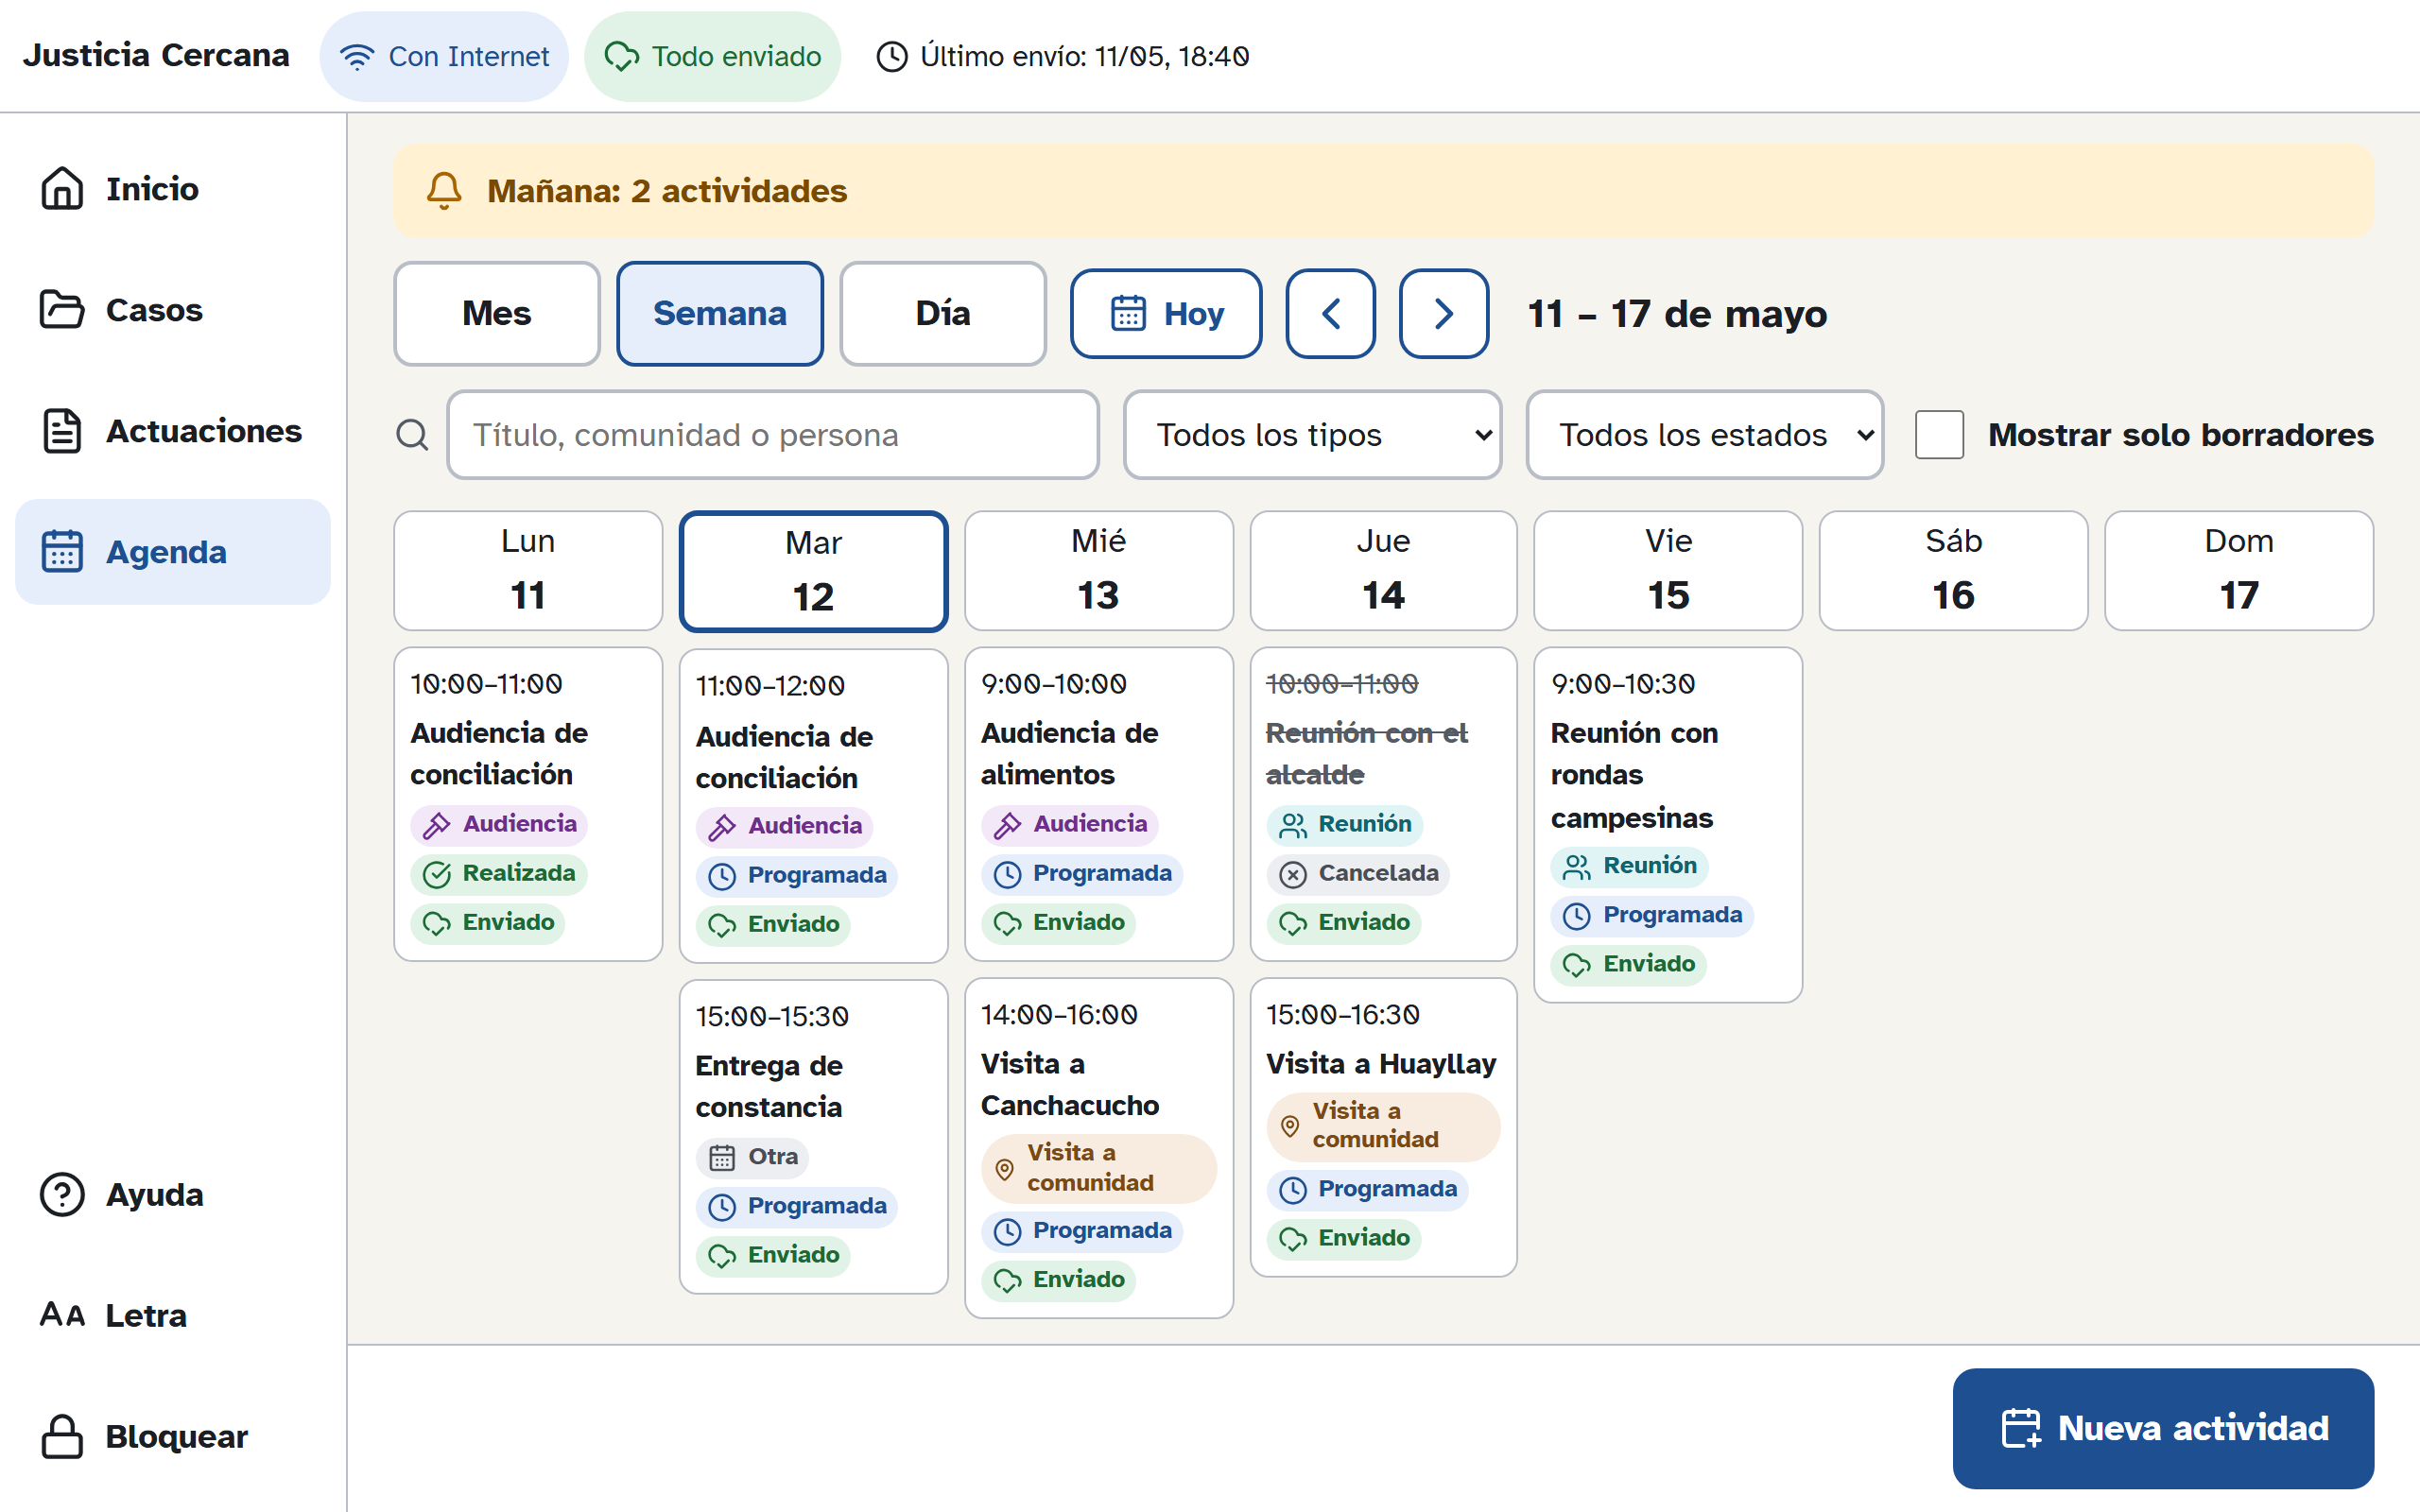
\includegraphics[width=\linewidth]{../../captures/F3-02_agenda-semana.png}\\[-2pt]{\footnotesize\raggedright\textbf{P-07 · 2.} Vista Semana: categorías con color + ícono + texto y estados \emph{(Cobertura y funcionamiento de los módulos)}\par}\end{minipage}\par\vspace{8pt}\noindent
\begin{minipage}[t]{0.49\textwidth}\centering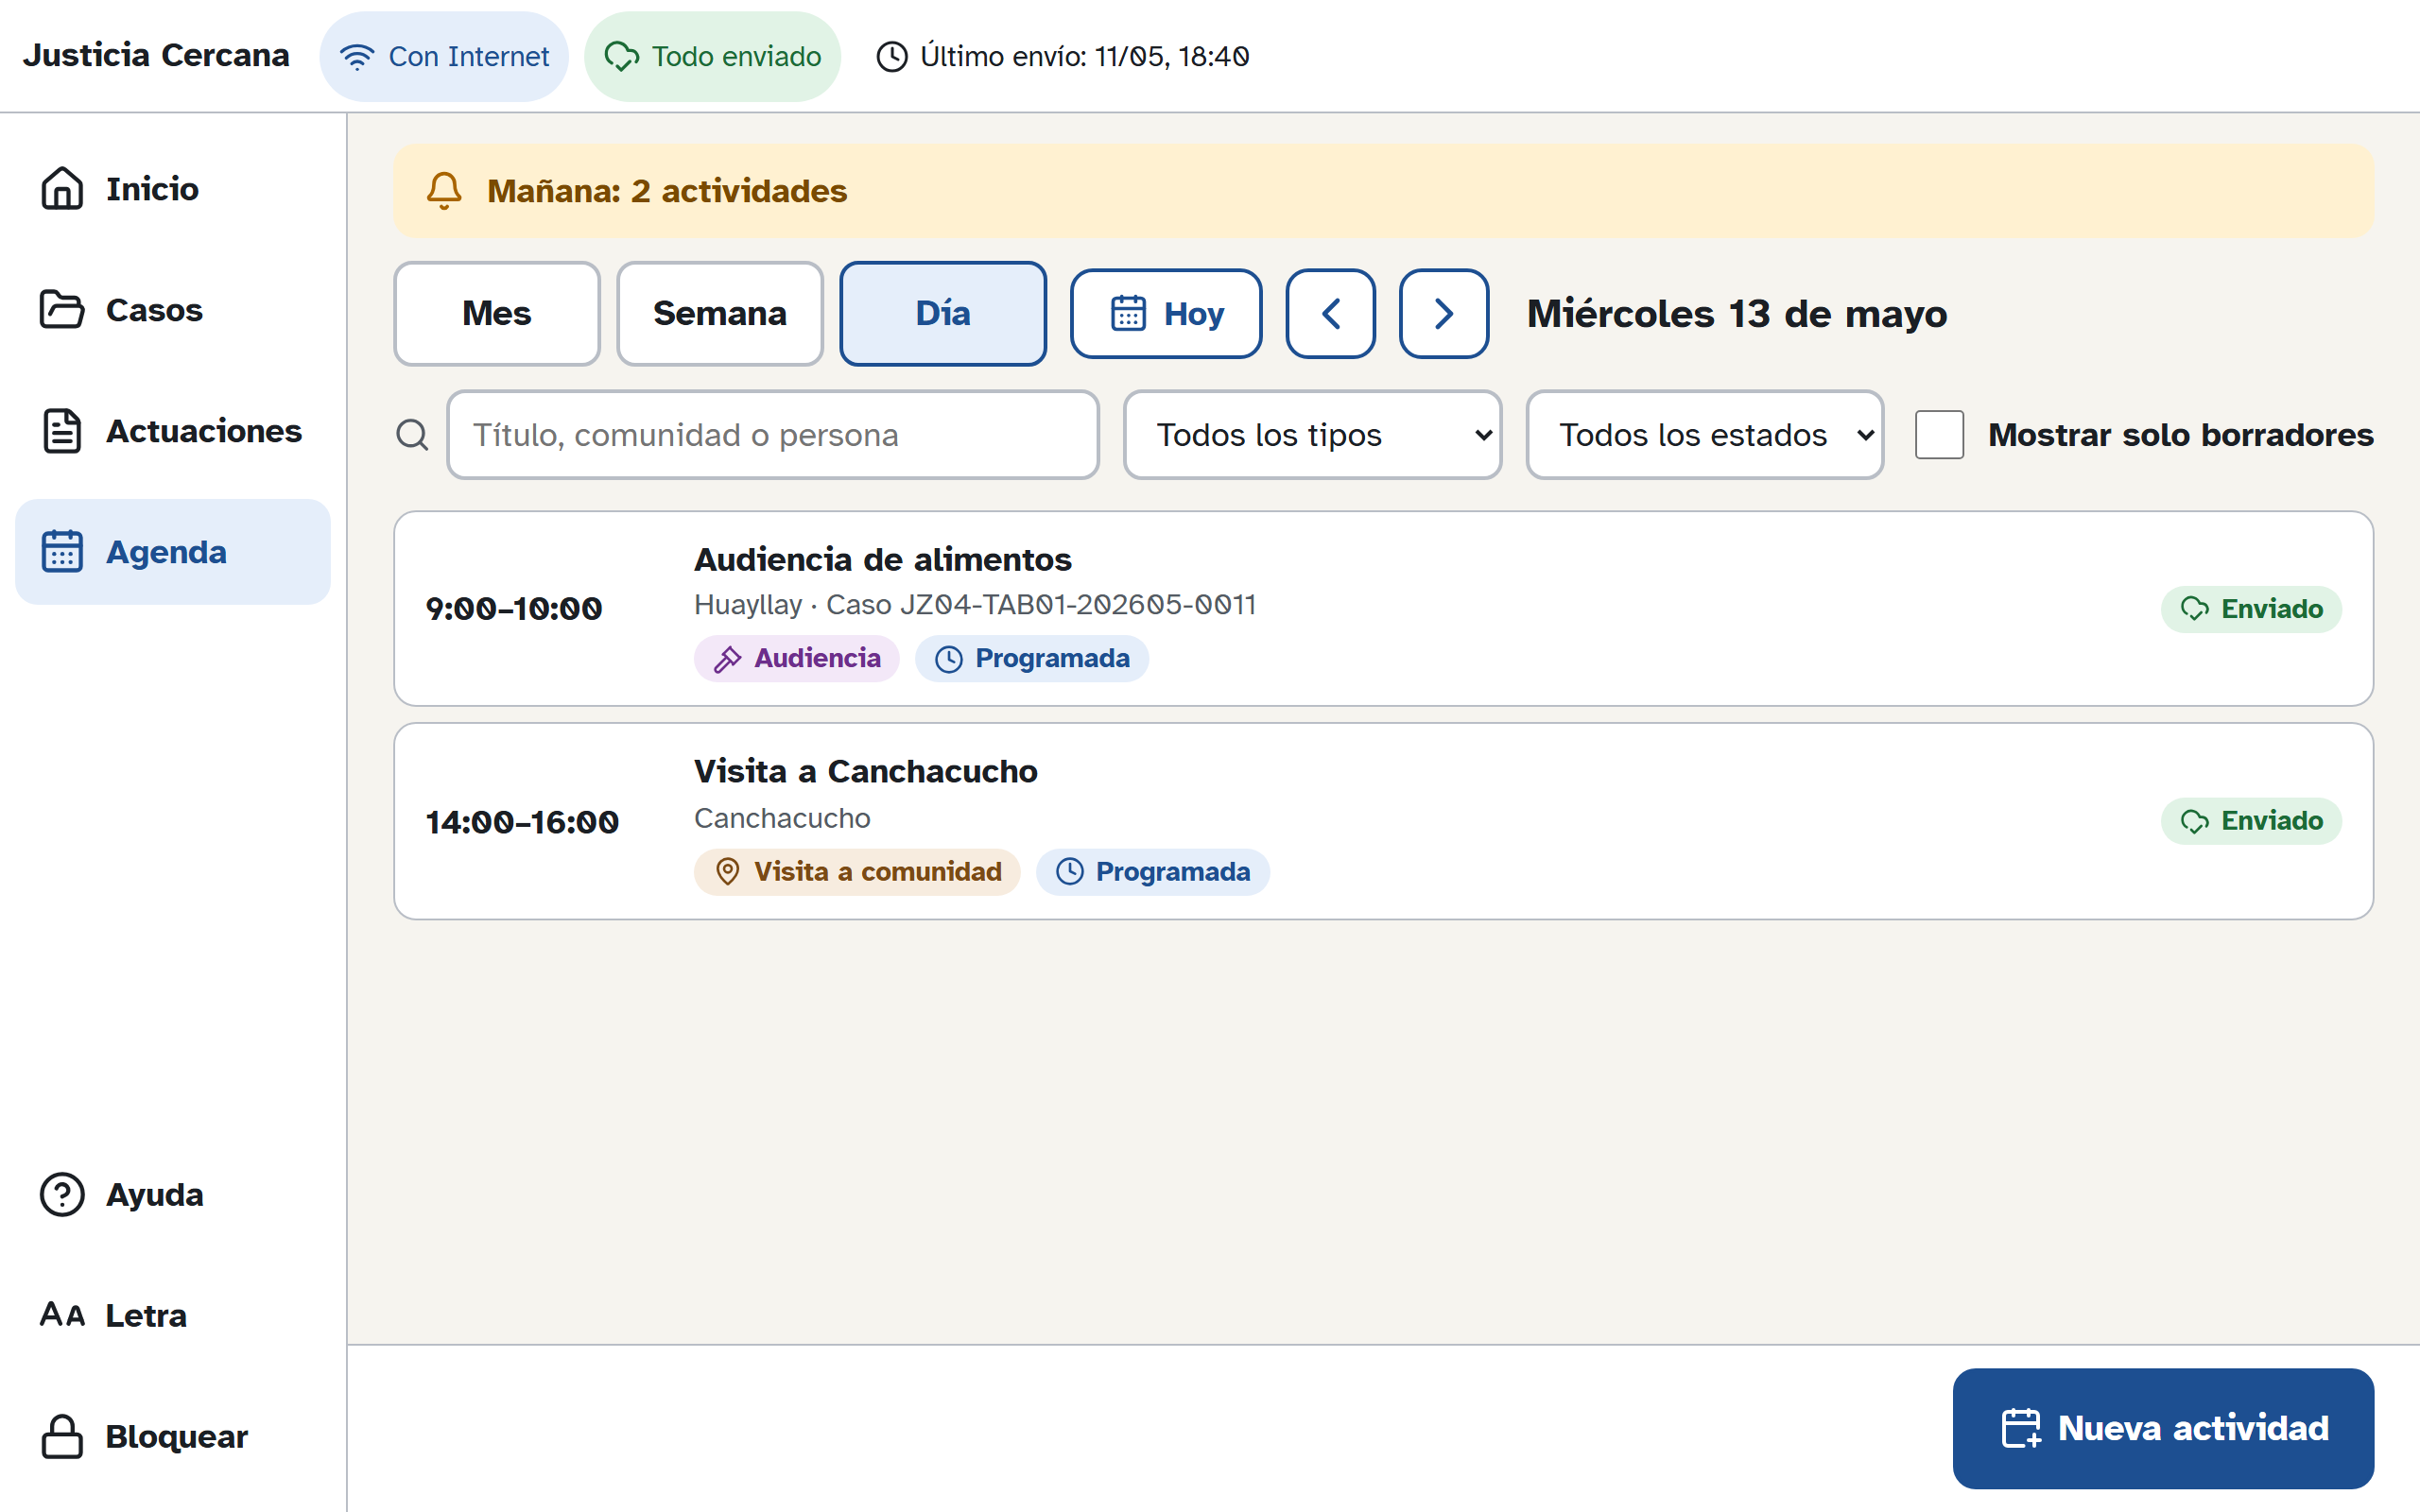
\includegraphics[width=\linewidth]{../../captures/F3-03a_agenda-dia-miercoles.png}\\[-2pt]{\footnotesize\raggedright\textbf{P-07 · 3.} Vista Día del miércoles con detalle \emph{(Cobertura y funcionamiento de los módulos)}\par}\end{minipage}\hfill
\begin{minipage}[t]{0.49\textwidth}\centering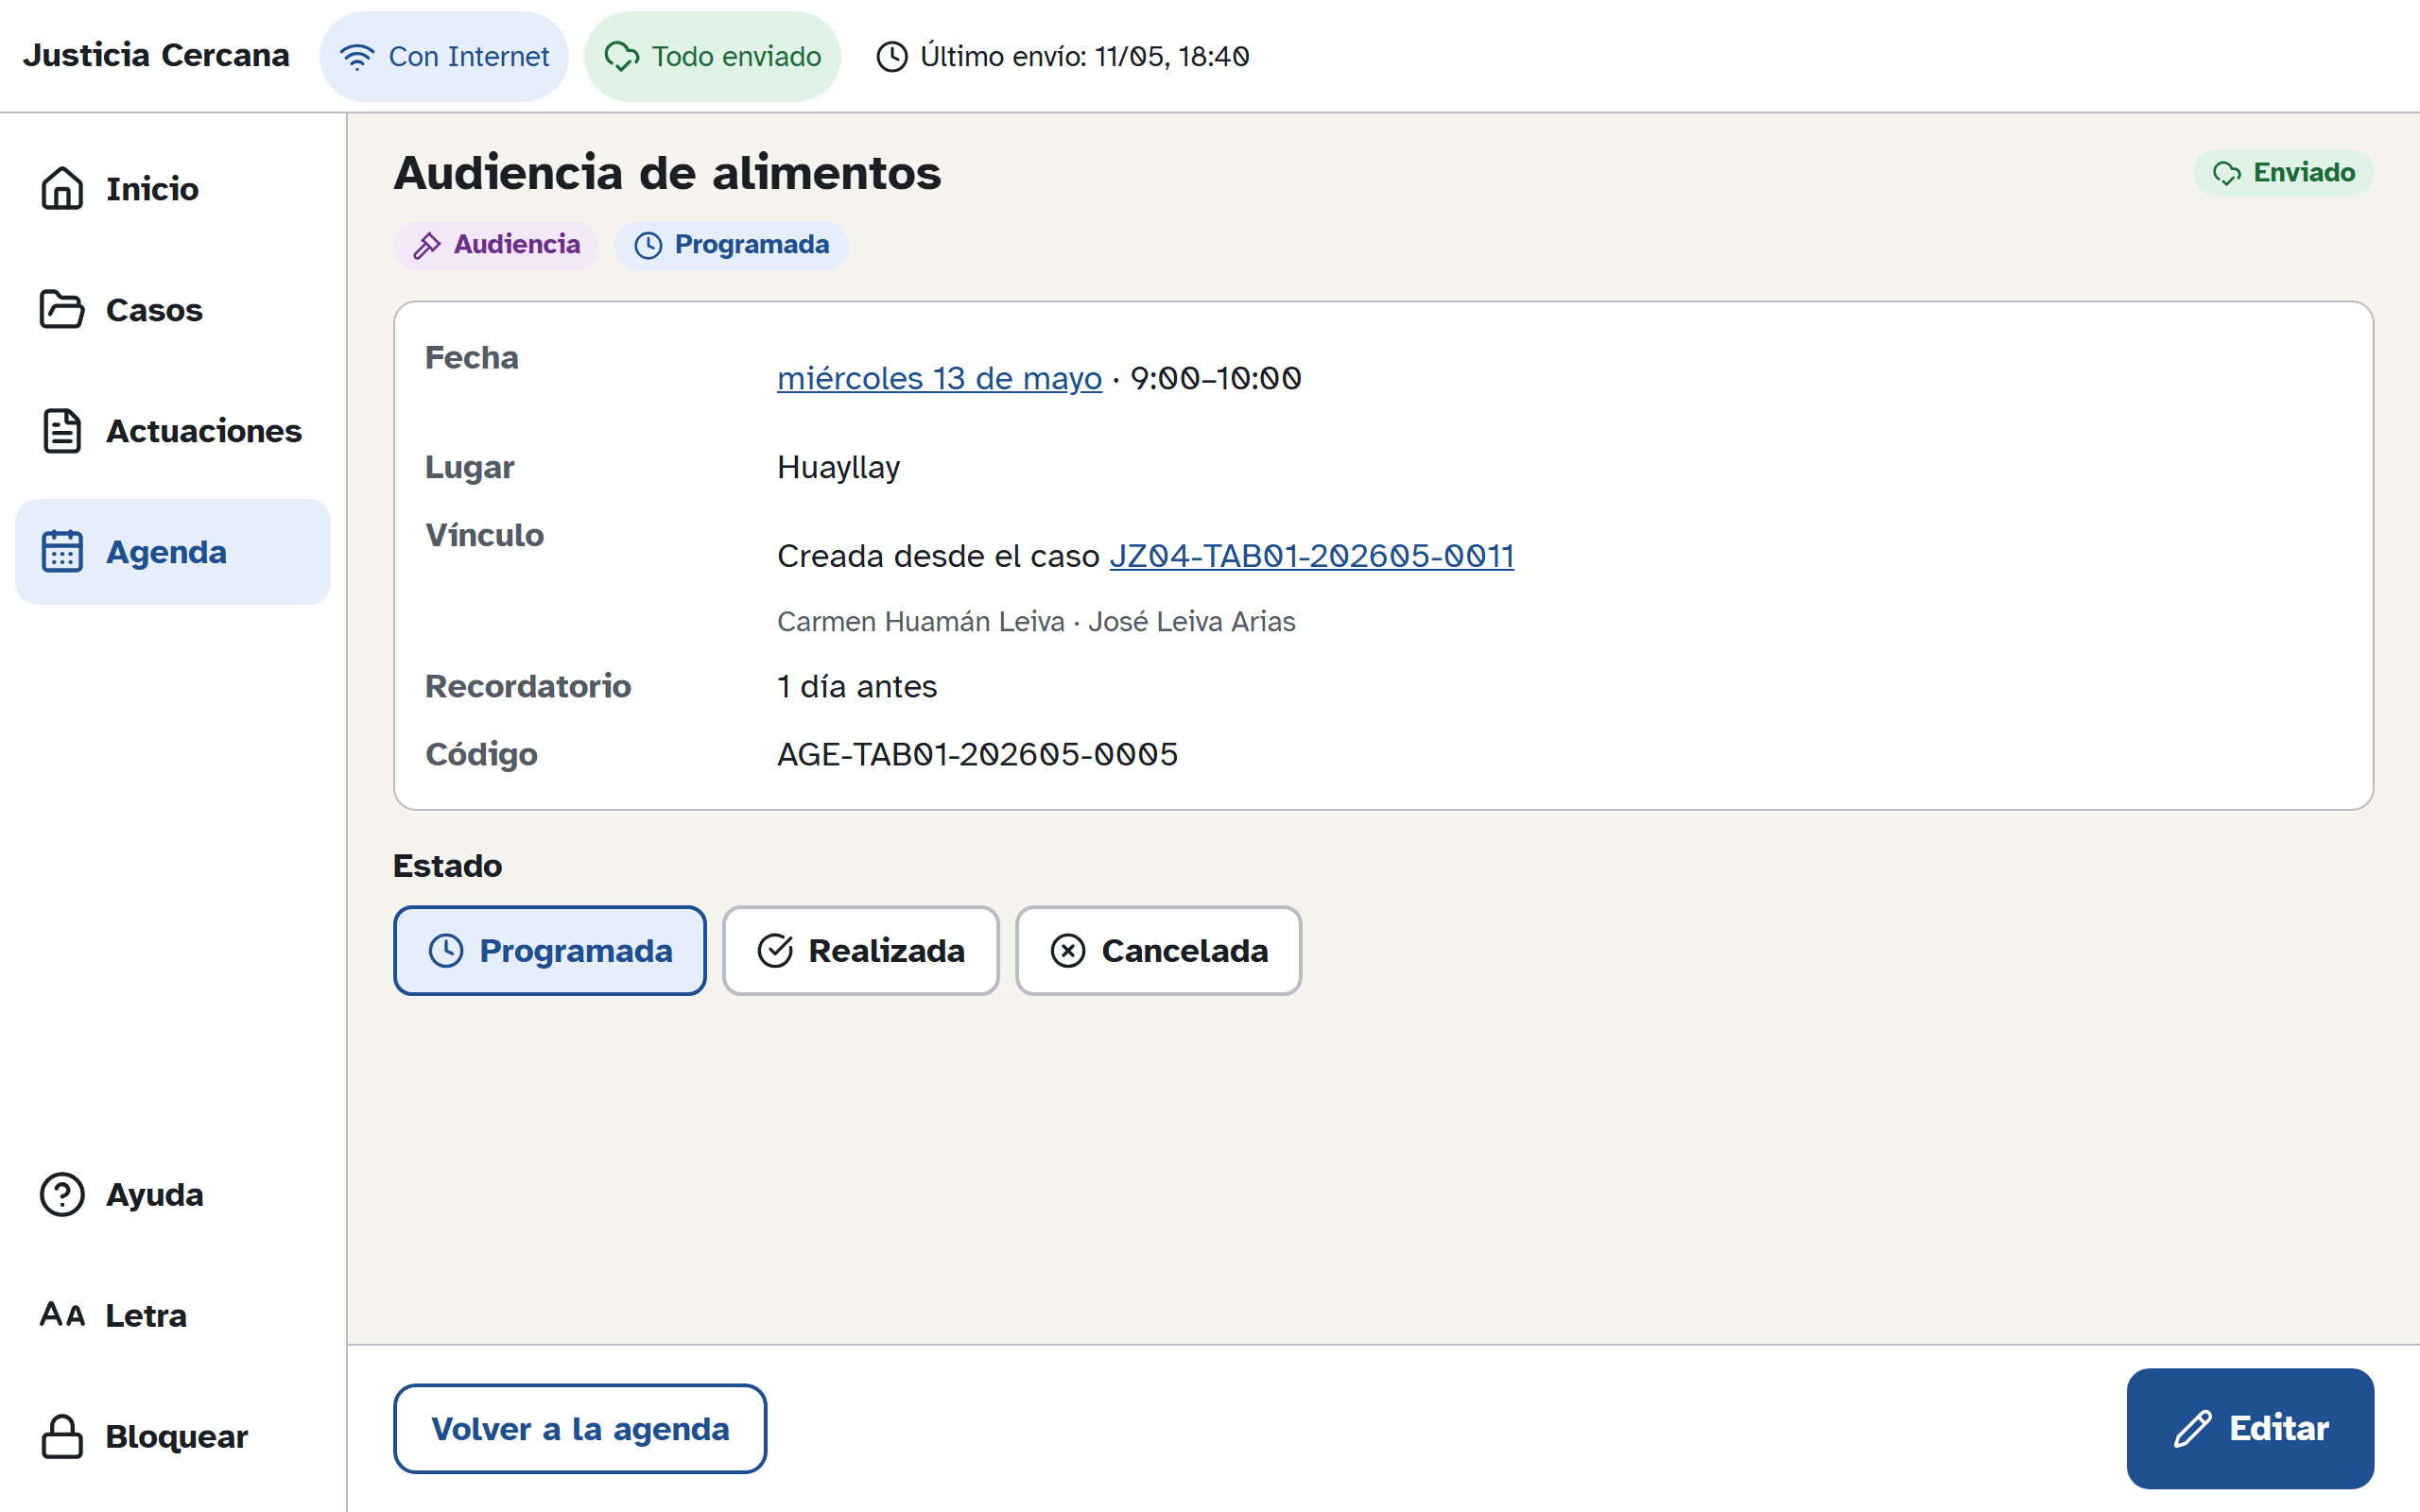
\includegraphics[width=\linewidth]{../../captures/F3-03b_detalle-vinculo-caso.png}\\[-2pt]{\footnotesize\raggedright\textbf{P-08 · 3.} Detalle de la actividad con vínculo al caso \emph{(Cobertura y funcionamiento de los módulos)}\par}\end{minipage}\par\vspace{8pt}\noindent
\par\vspace{4pt}
\subsection*{Flujo 4}
\noindent
\begin{minipage}[t]{0.49\textwidth}\centering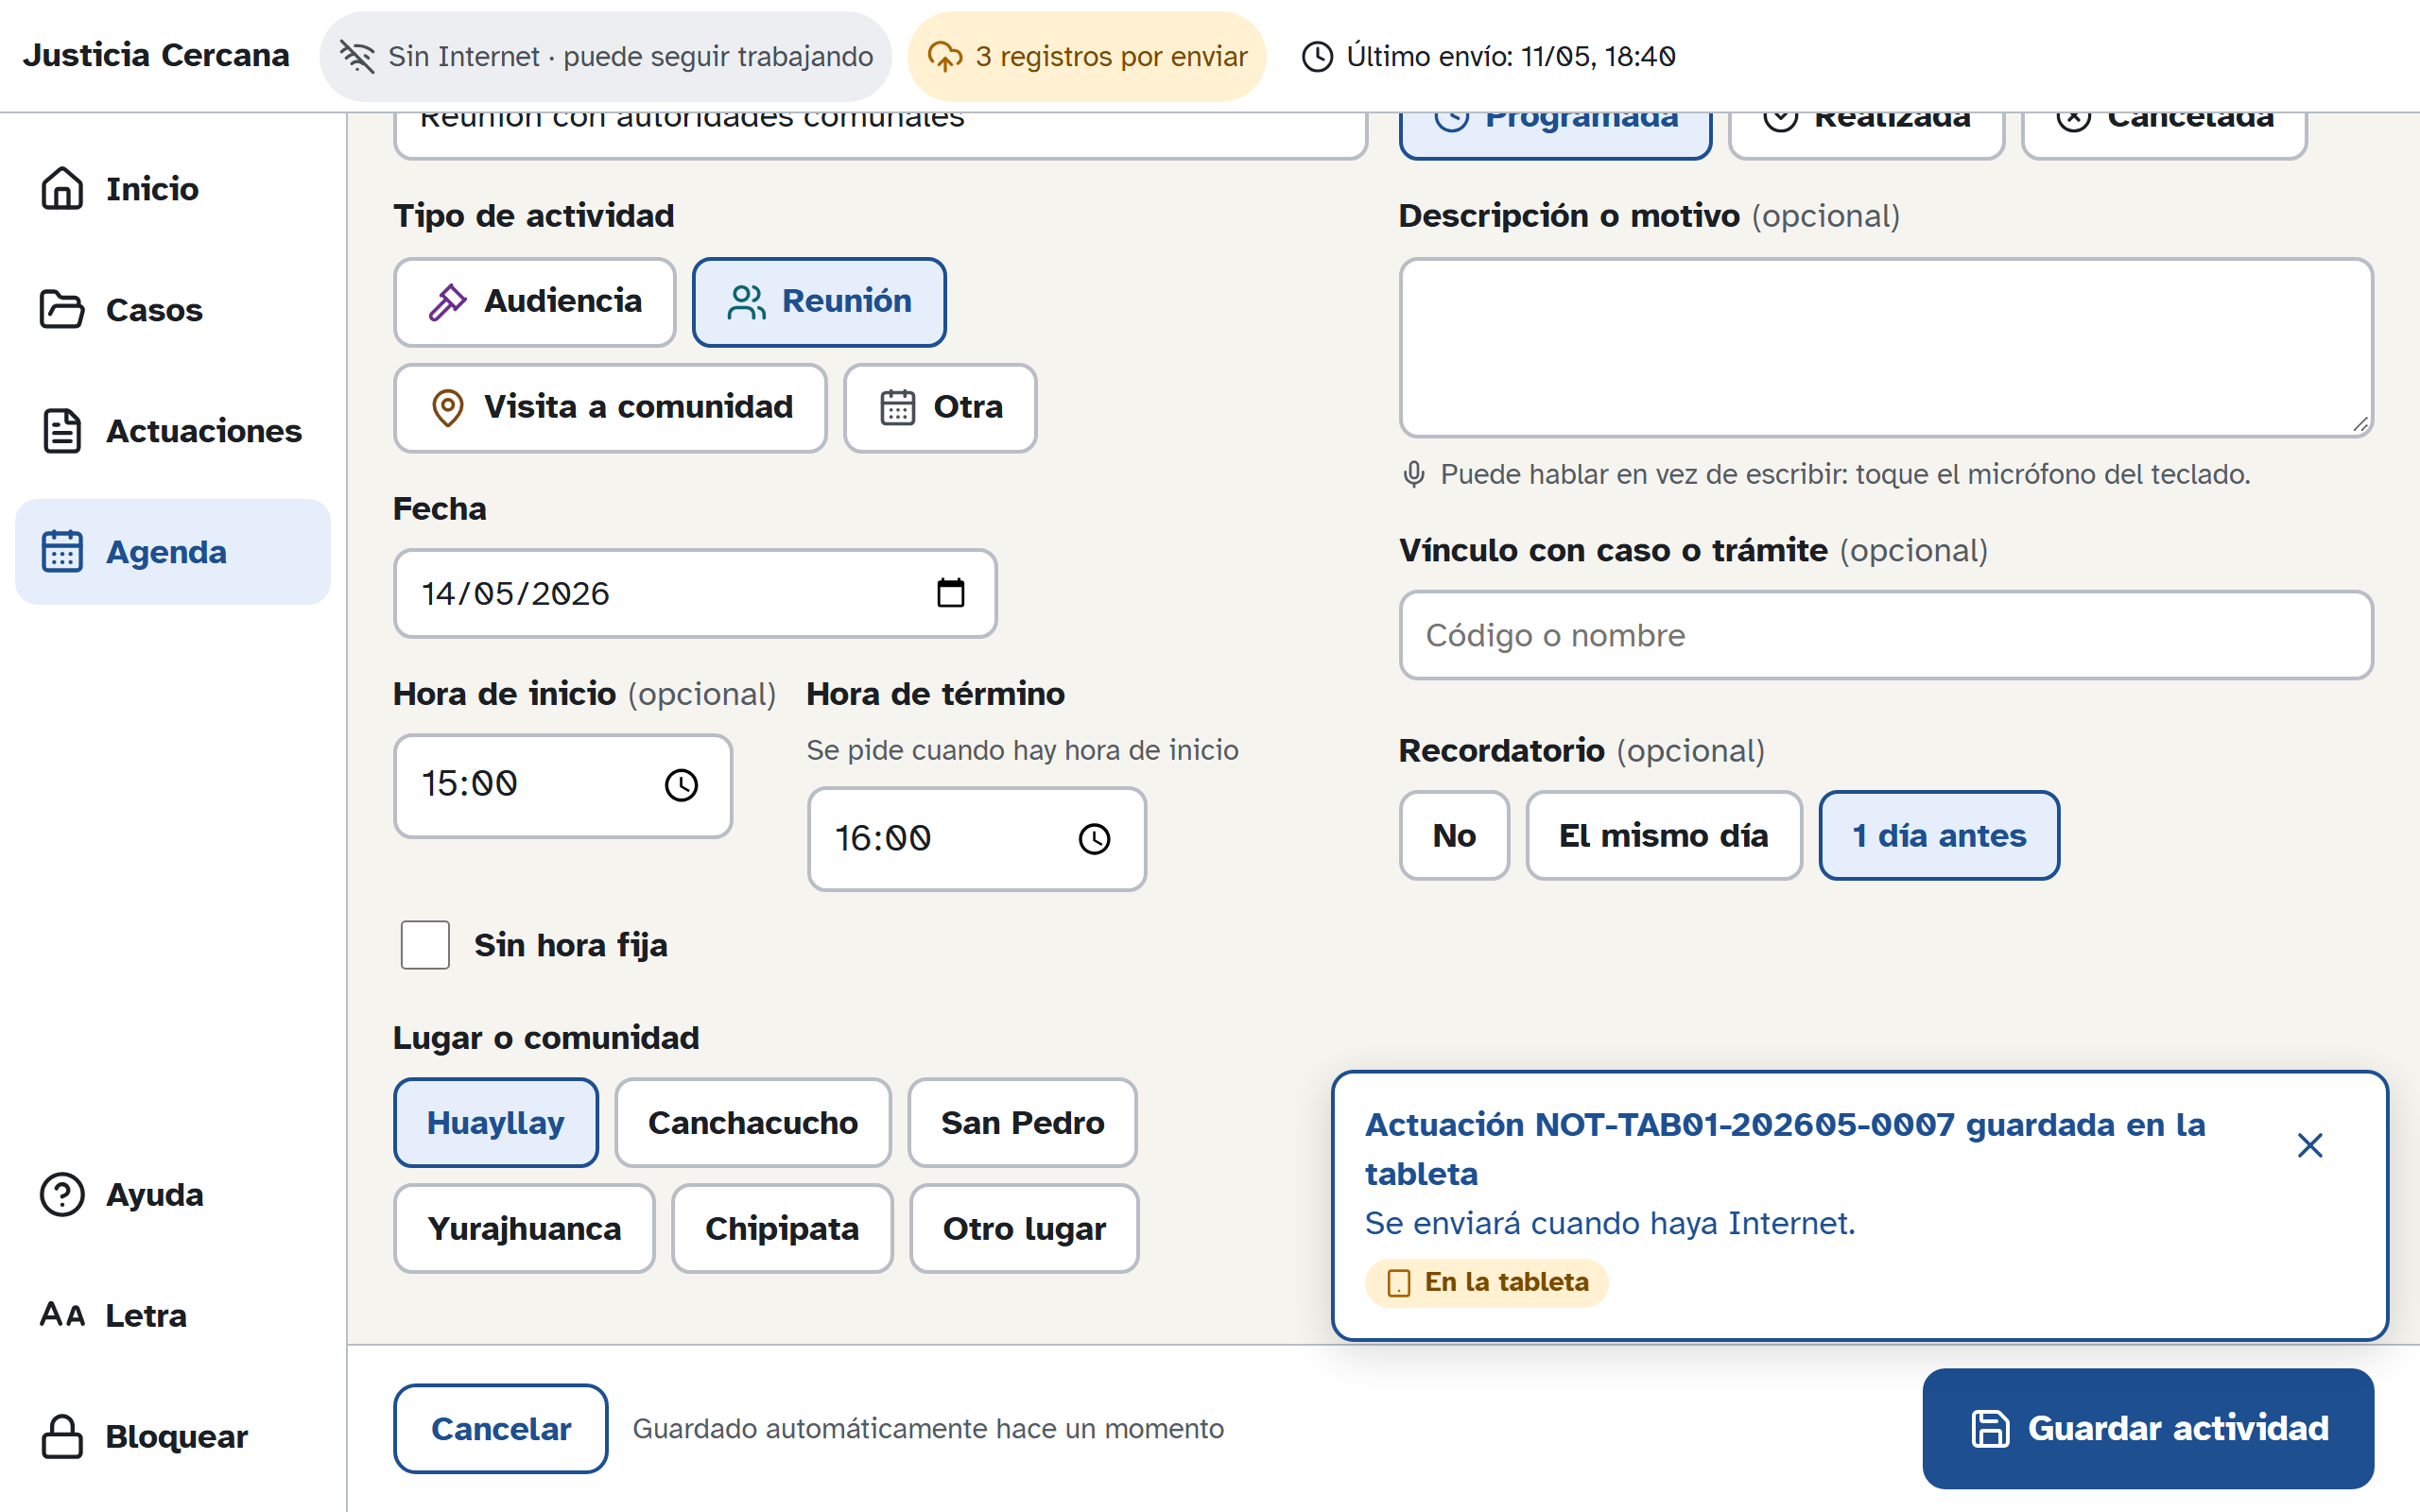
\includegraphics[width=\linewidth]{../../captures/F4-01_nueva-actividad.png}\\[-2pt]{\footnotesize\raggedright\textbf{P-08 · 1.} Reunión con autoridades comunales, jueves 14/05 15:00–16:00, Huayllay \emph{(Cobertura y funcionamiento de los módulos)}\par}\end{minipage}\hfill
\begin{minipage}[t]{0.49\textwidth}\centering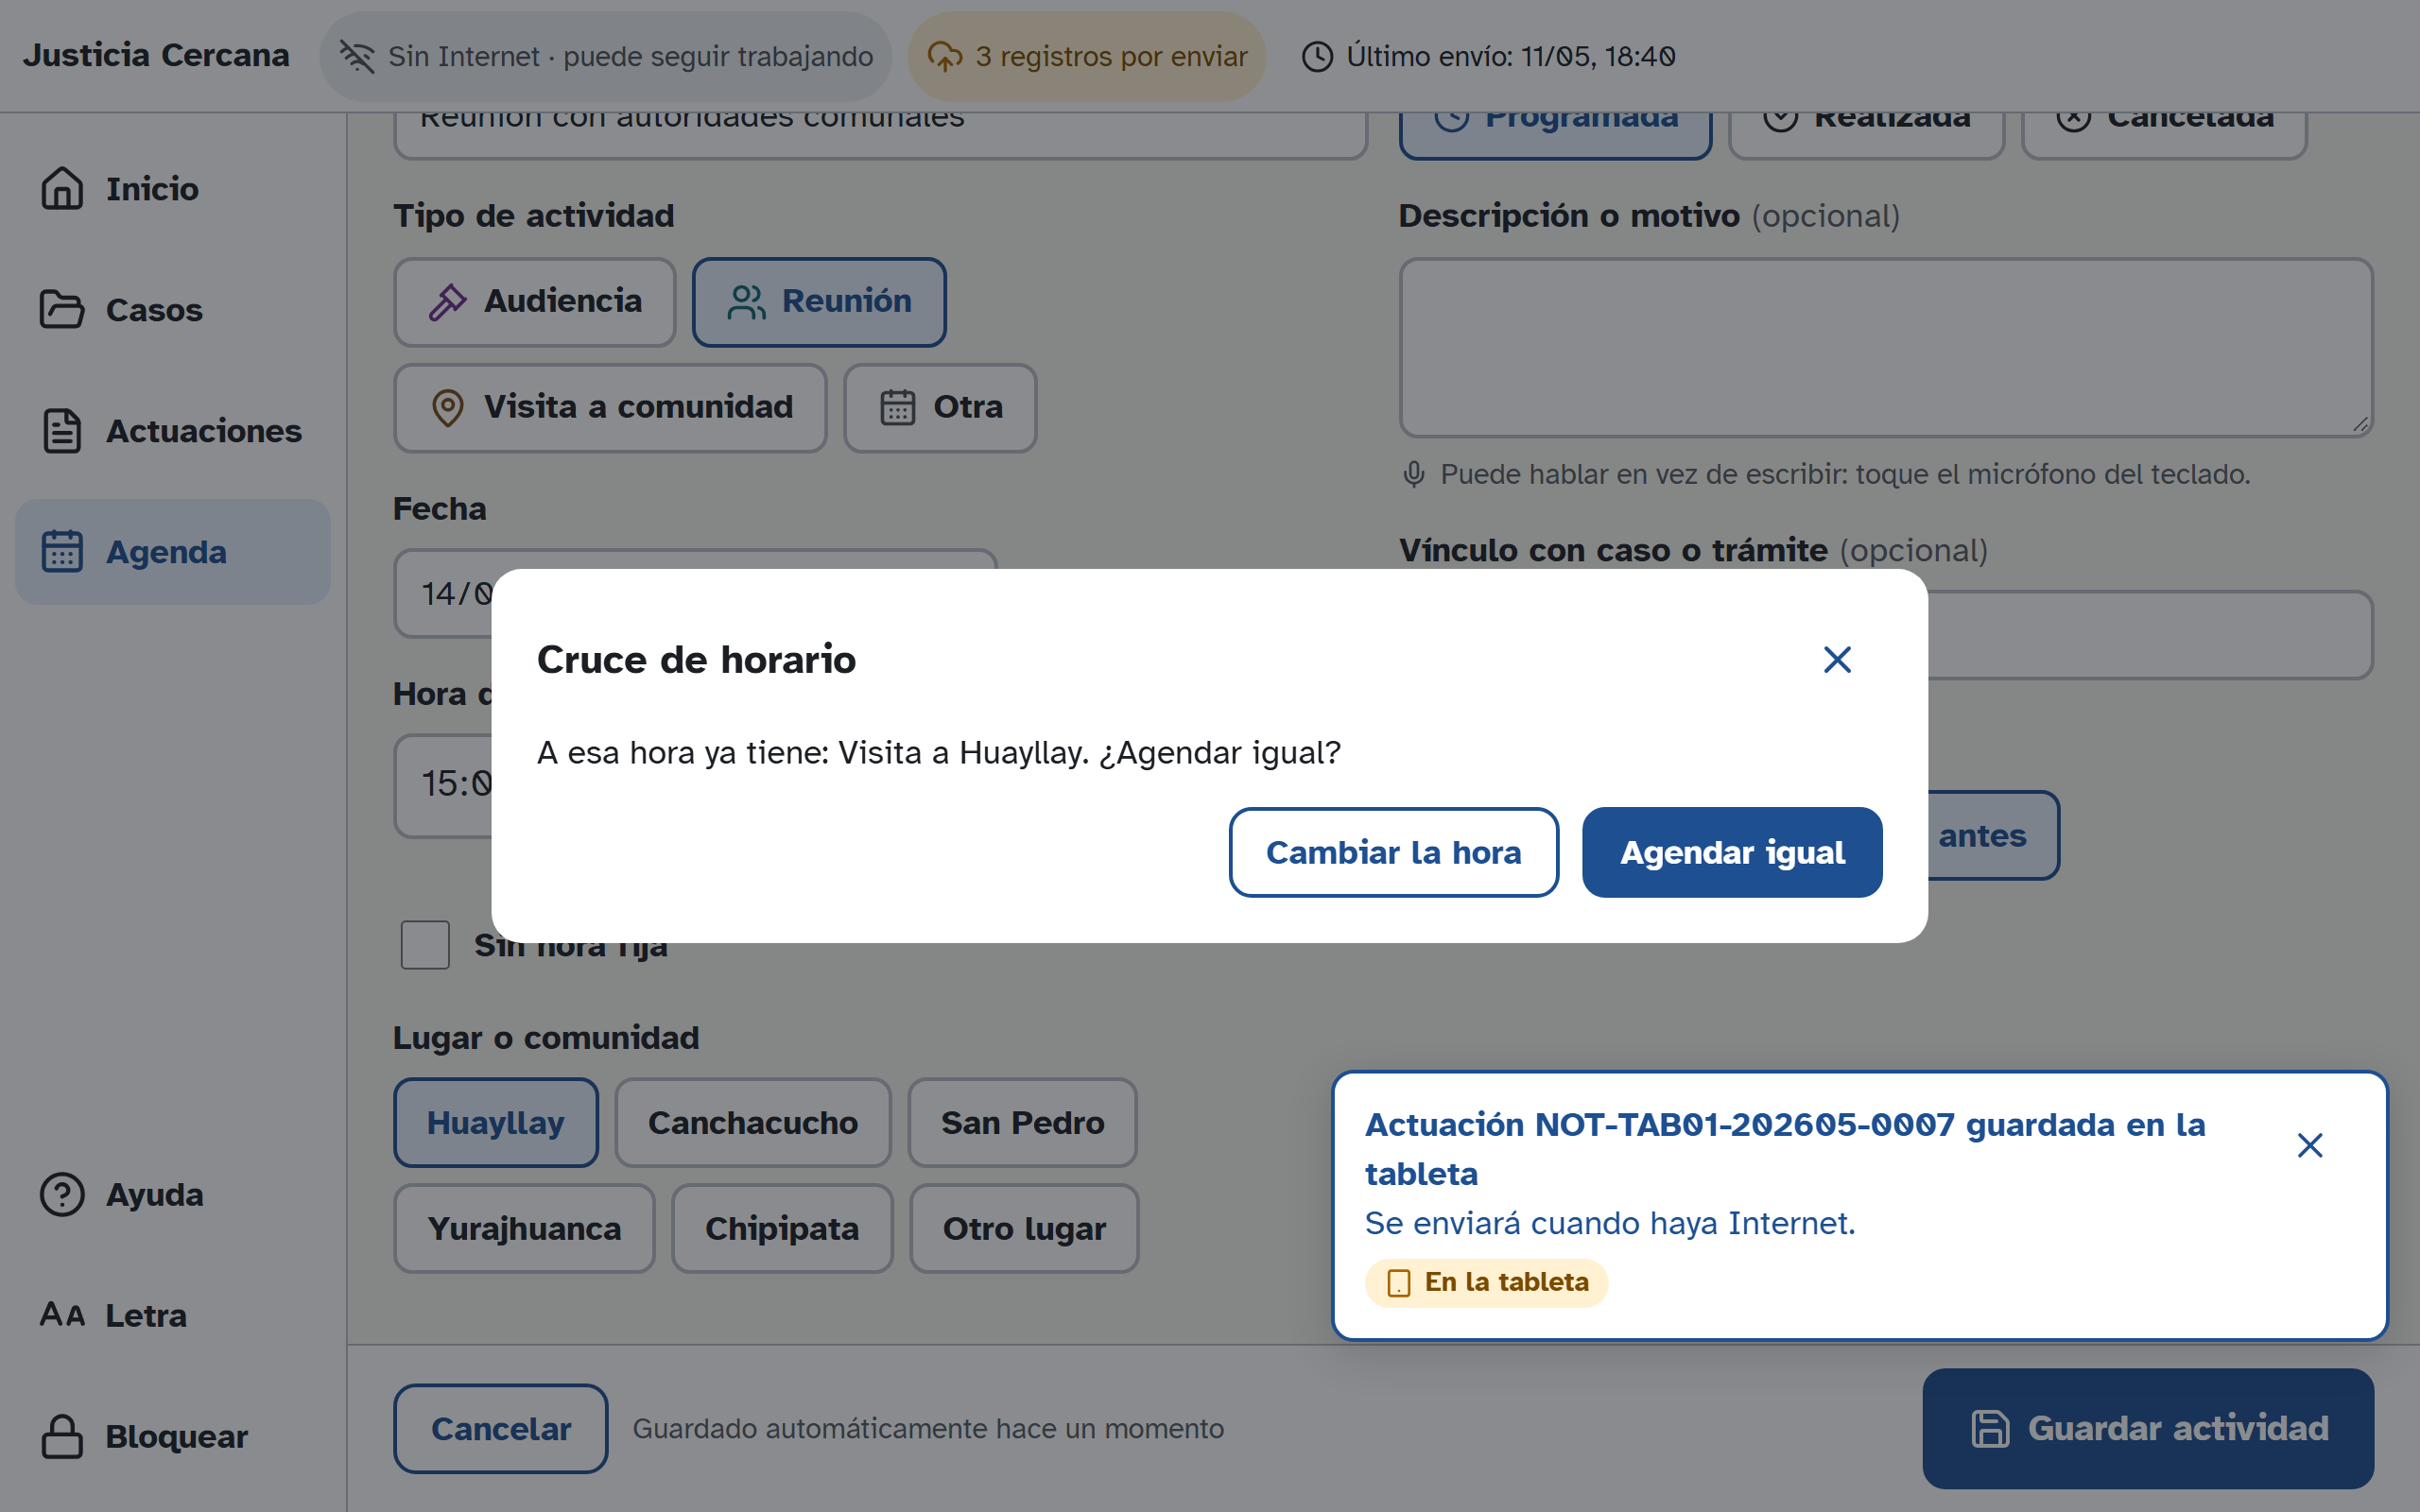
\includegraphics[width=\linewidth]{../../captures/F4-02a_cruce-horario.png}\\[-2pt]{\footnotesize\raggedright\textbf{P-08 · 2.} Aviso no bloqueante de cruce de horario con la otra actividad \emph{(Principios de diseño y heurísticas)}\par}\end{minipage}\par\vspace{8pt}\noindent
\begin{minipage}[t]{0.49\textwidth}\centering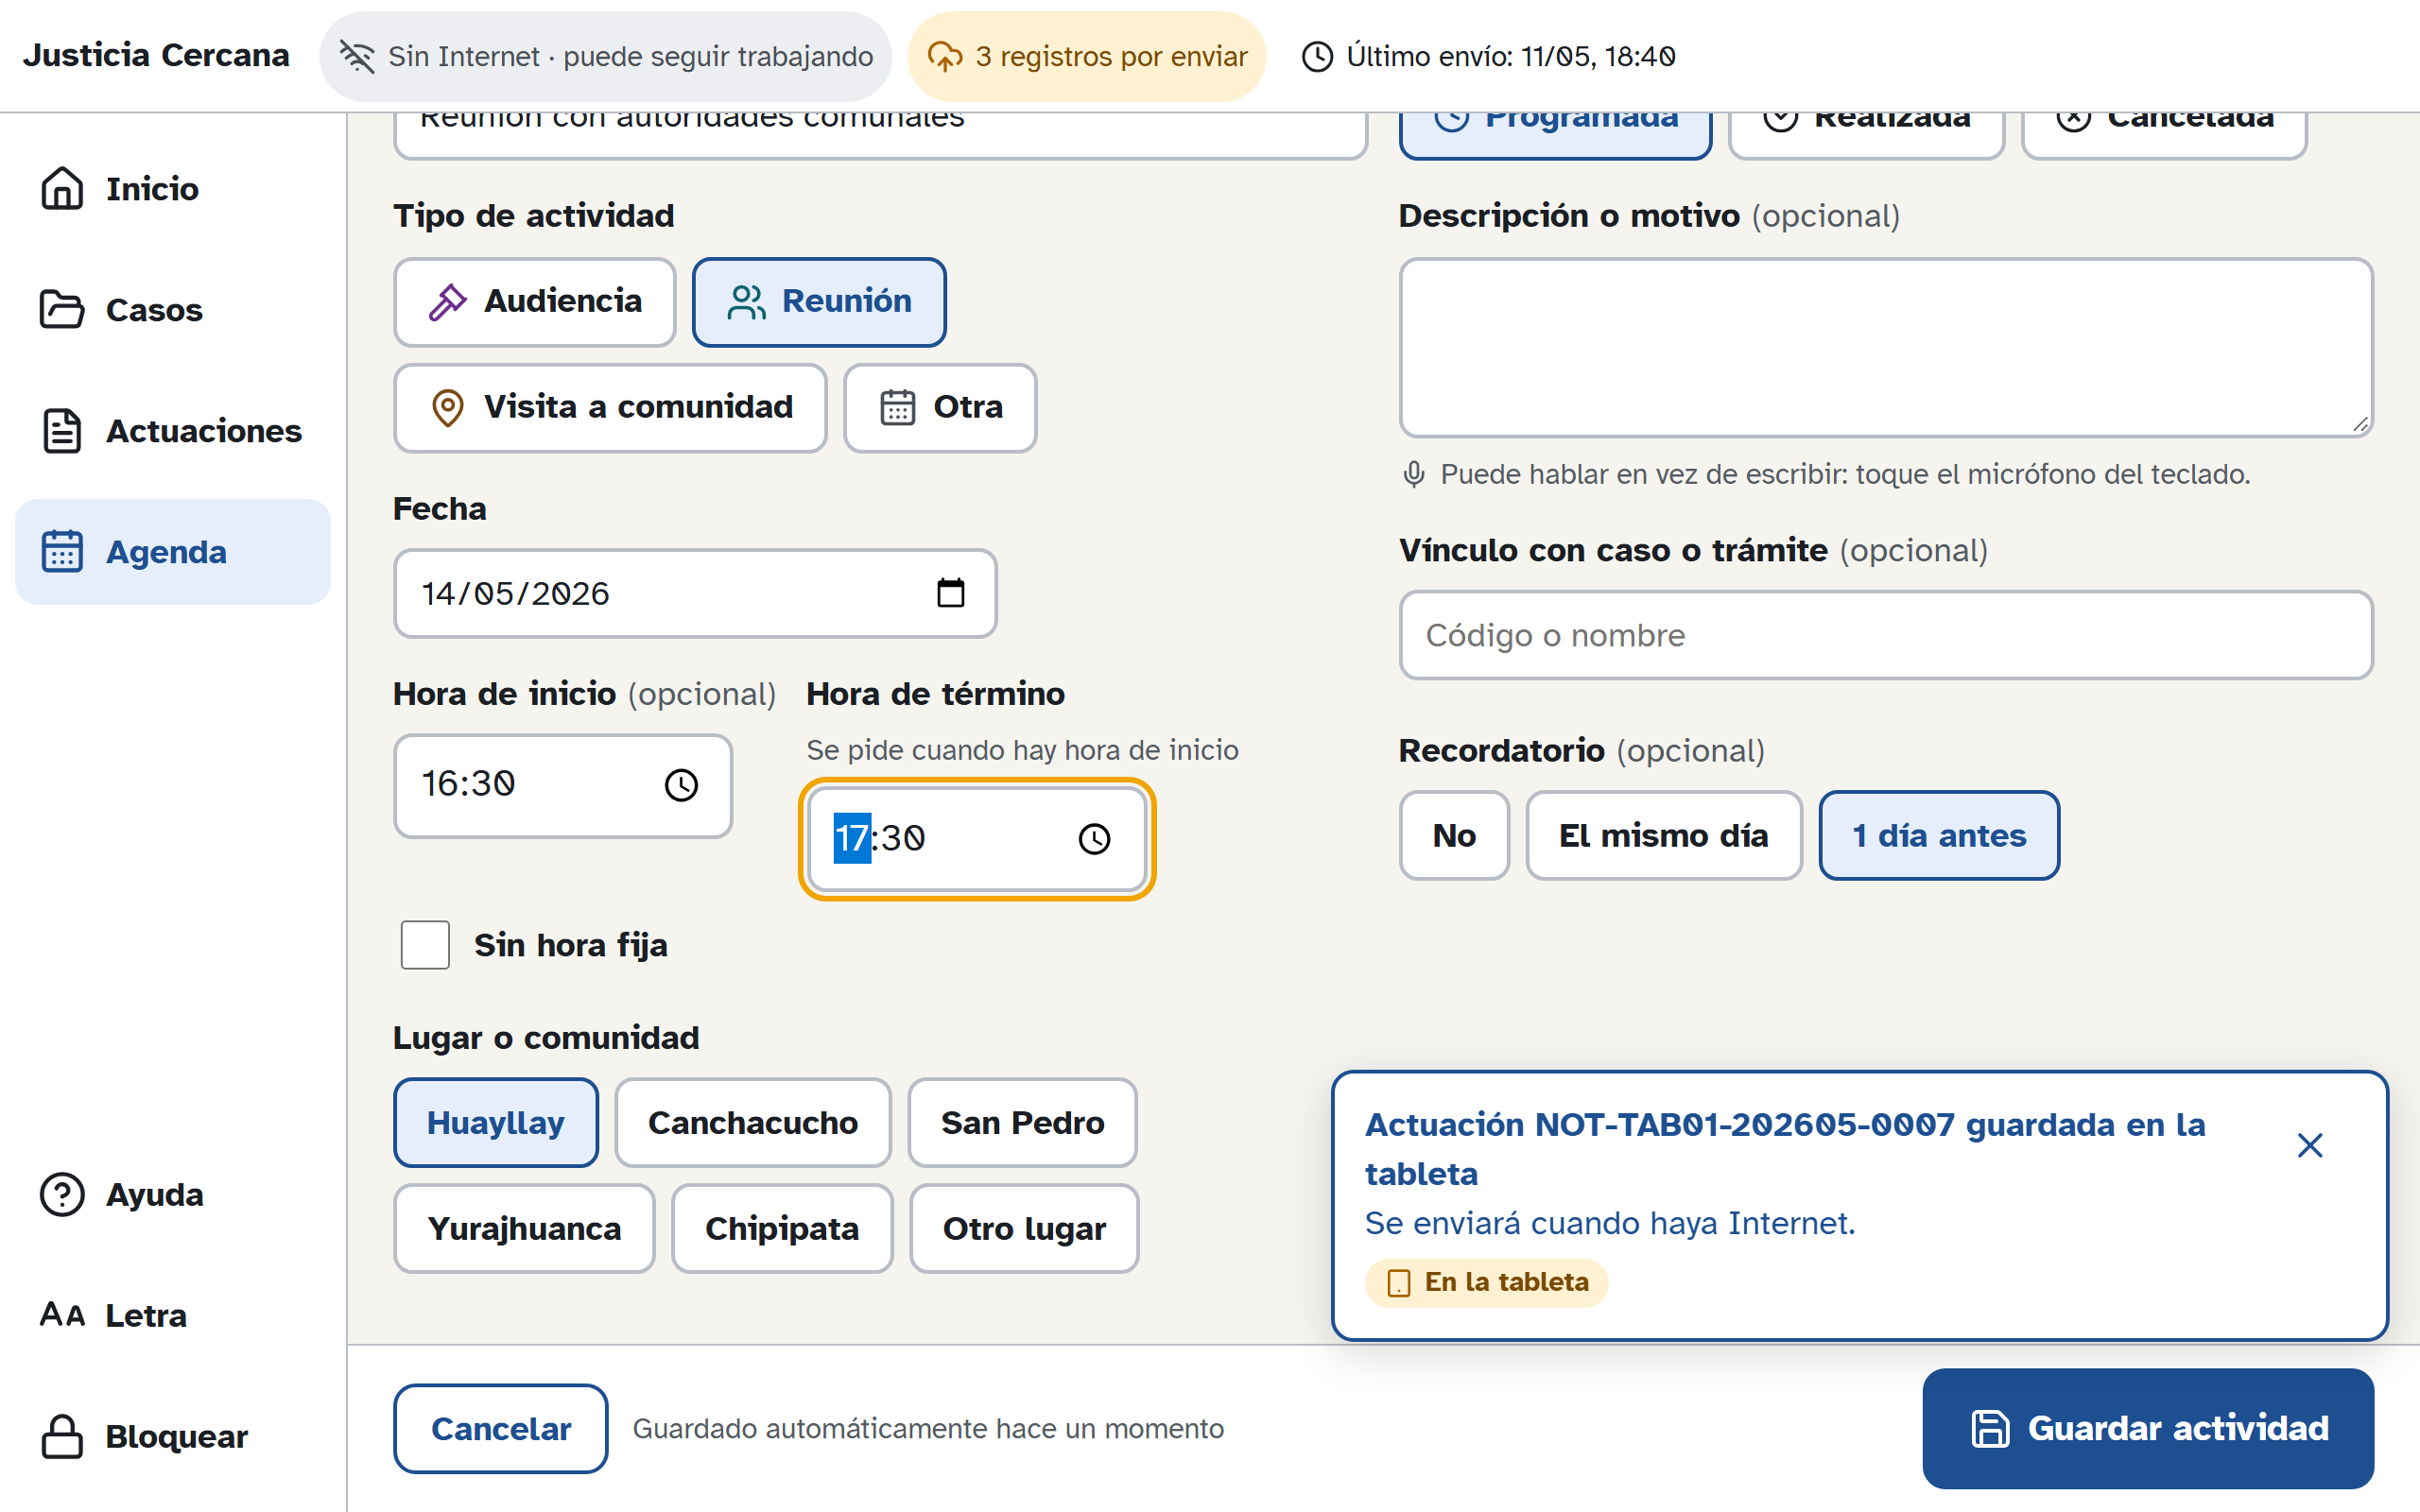
\includegraphics[width=\linewidth]{../../captures/F4-02b_hora-ajustada.png}\\[-2pt]{\footnotesize\raggedright\textbf{P-08 · 2.} Hora ajustada a 16:30–17:30 \emph{(Cobertura y funcionamiento de los módulos)}\par}\end{minipage}\hfill
\begin{minipage}[t]{0.49\textwidth}\centering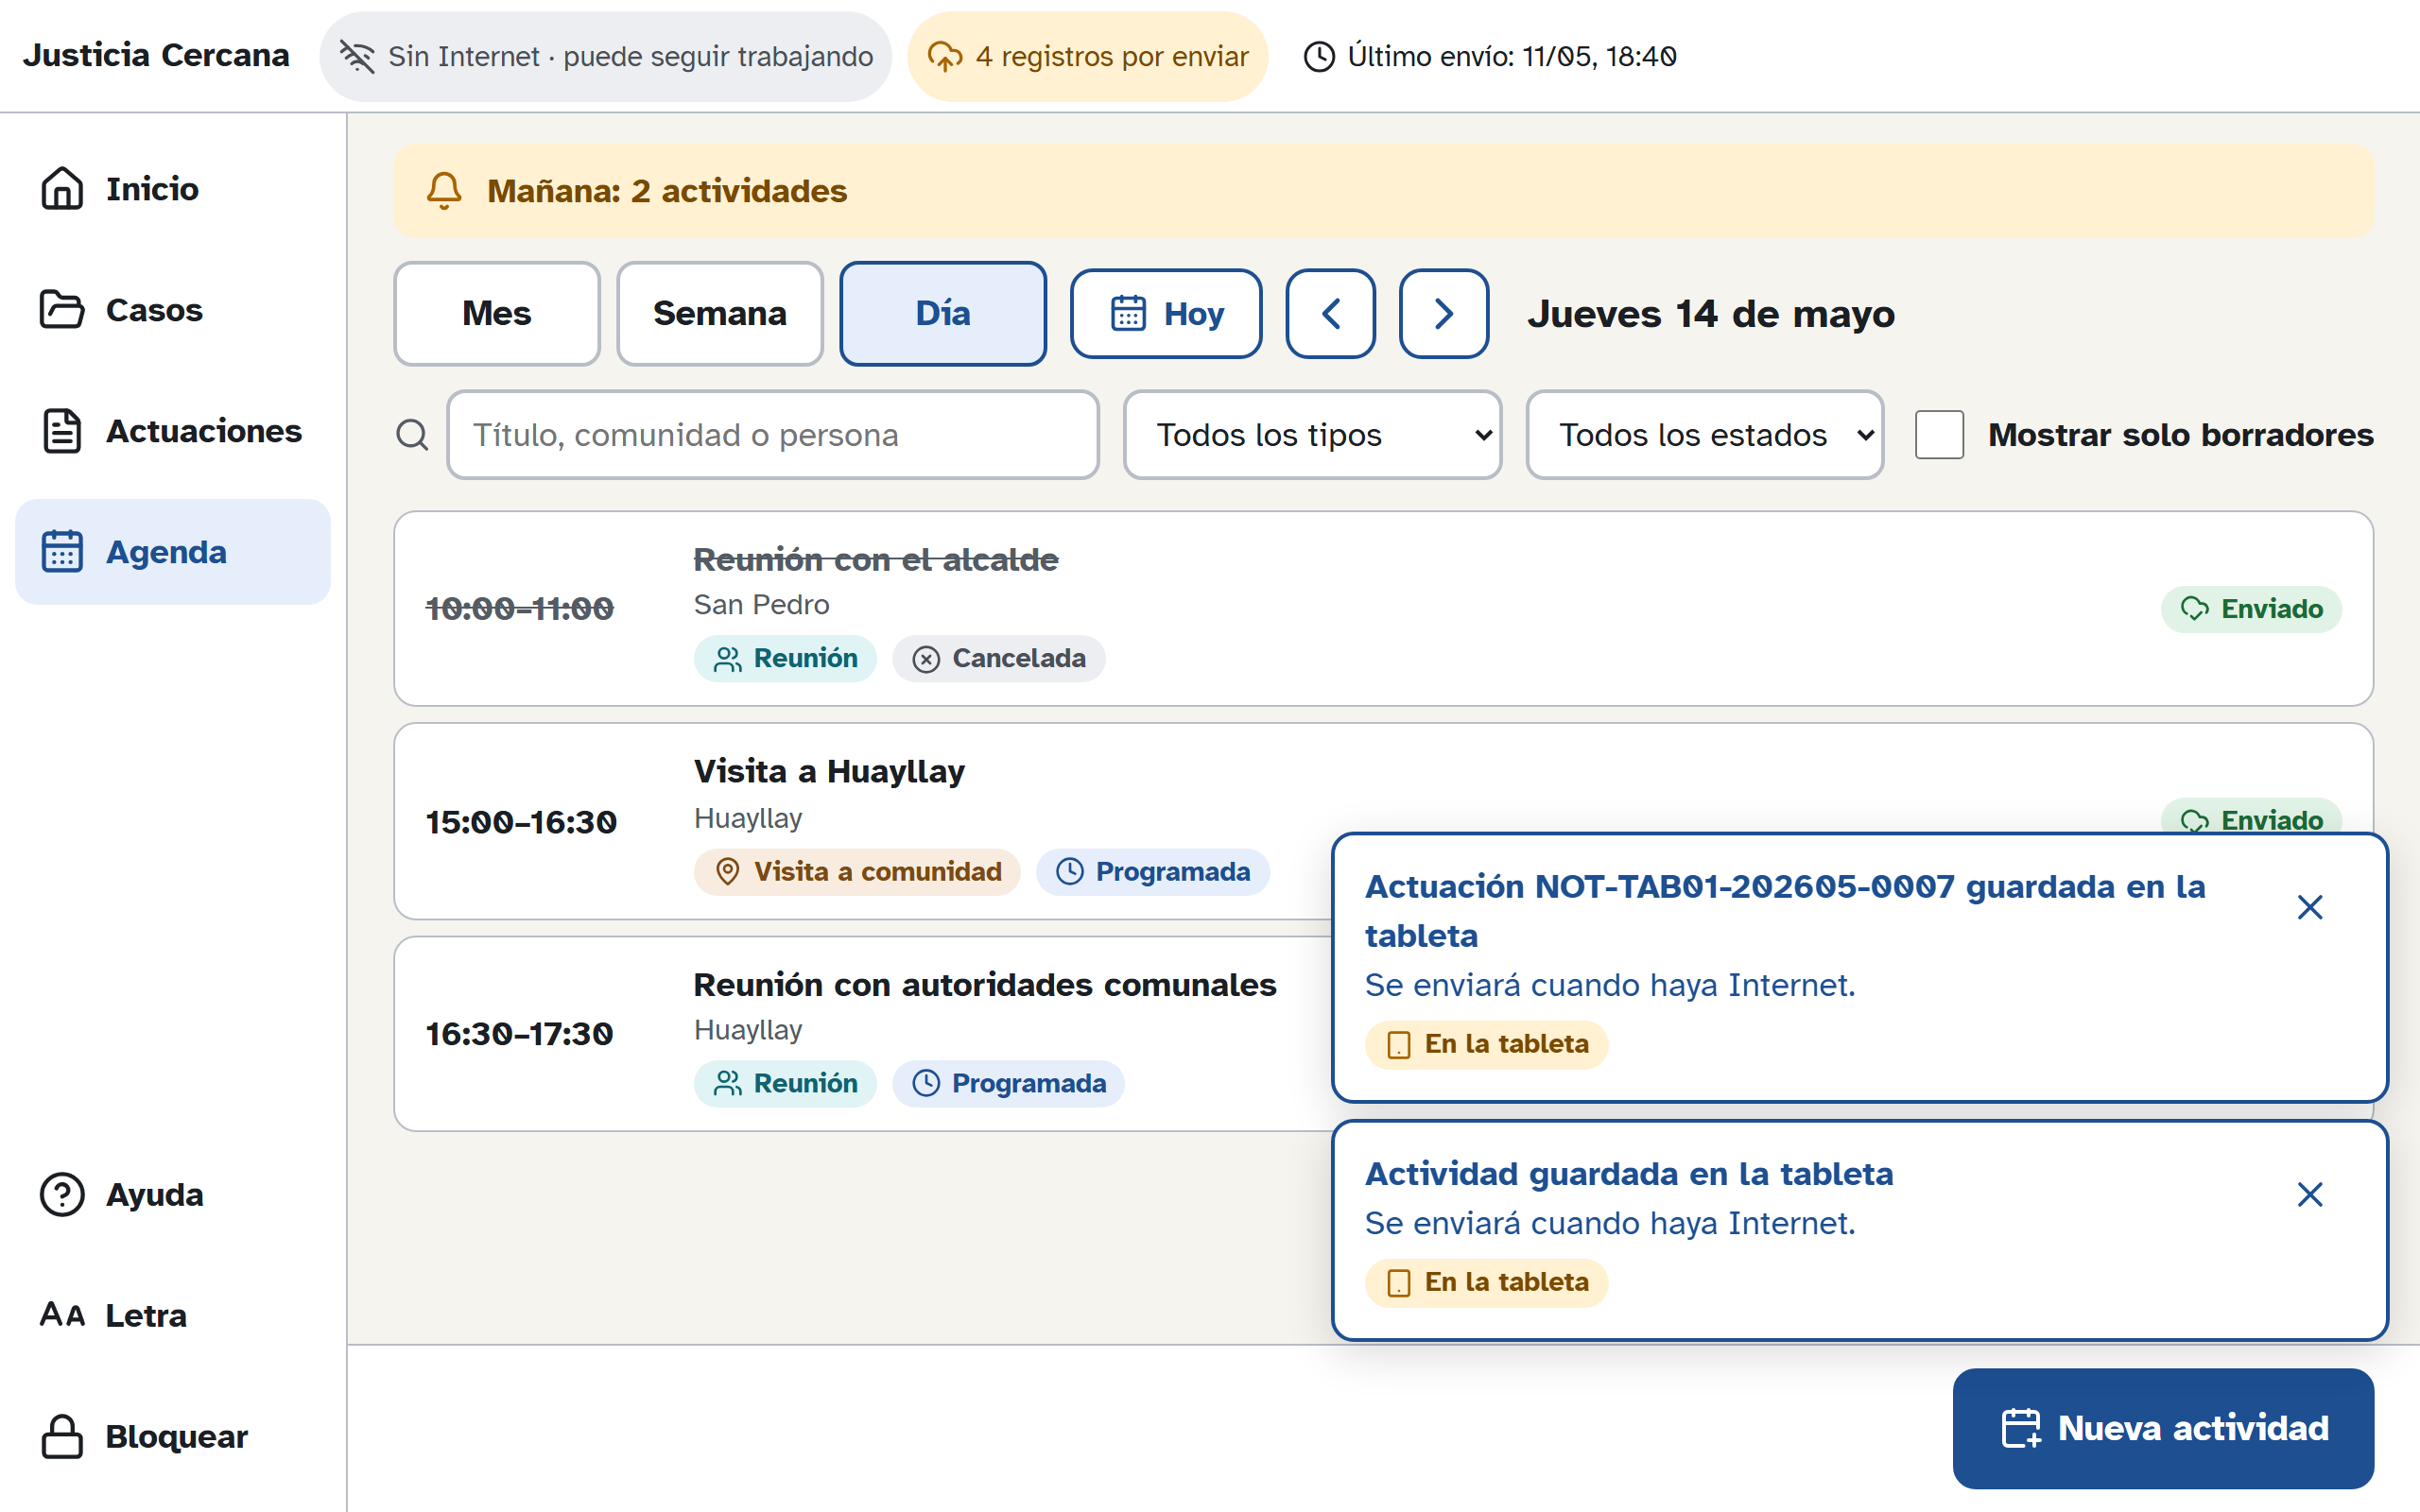
\includegraphics[width=\linewidth]{../../captures/F4-03_guardado-por-enviar.png}\\[-2pt]{\footnotesize\raggedright\textbf{P-07 · 3.} Guardada; barra ``4 registros por enviar'' \emph{(Funcionamiento sin conexión)}\par}\end{minipage}\par\vspace{8pt}\noindent
\begin{minipage}[t]{0.49\textwidth}\centering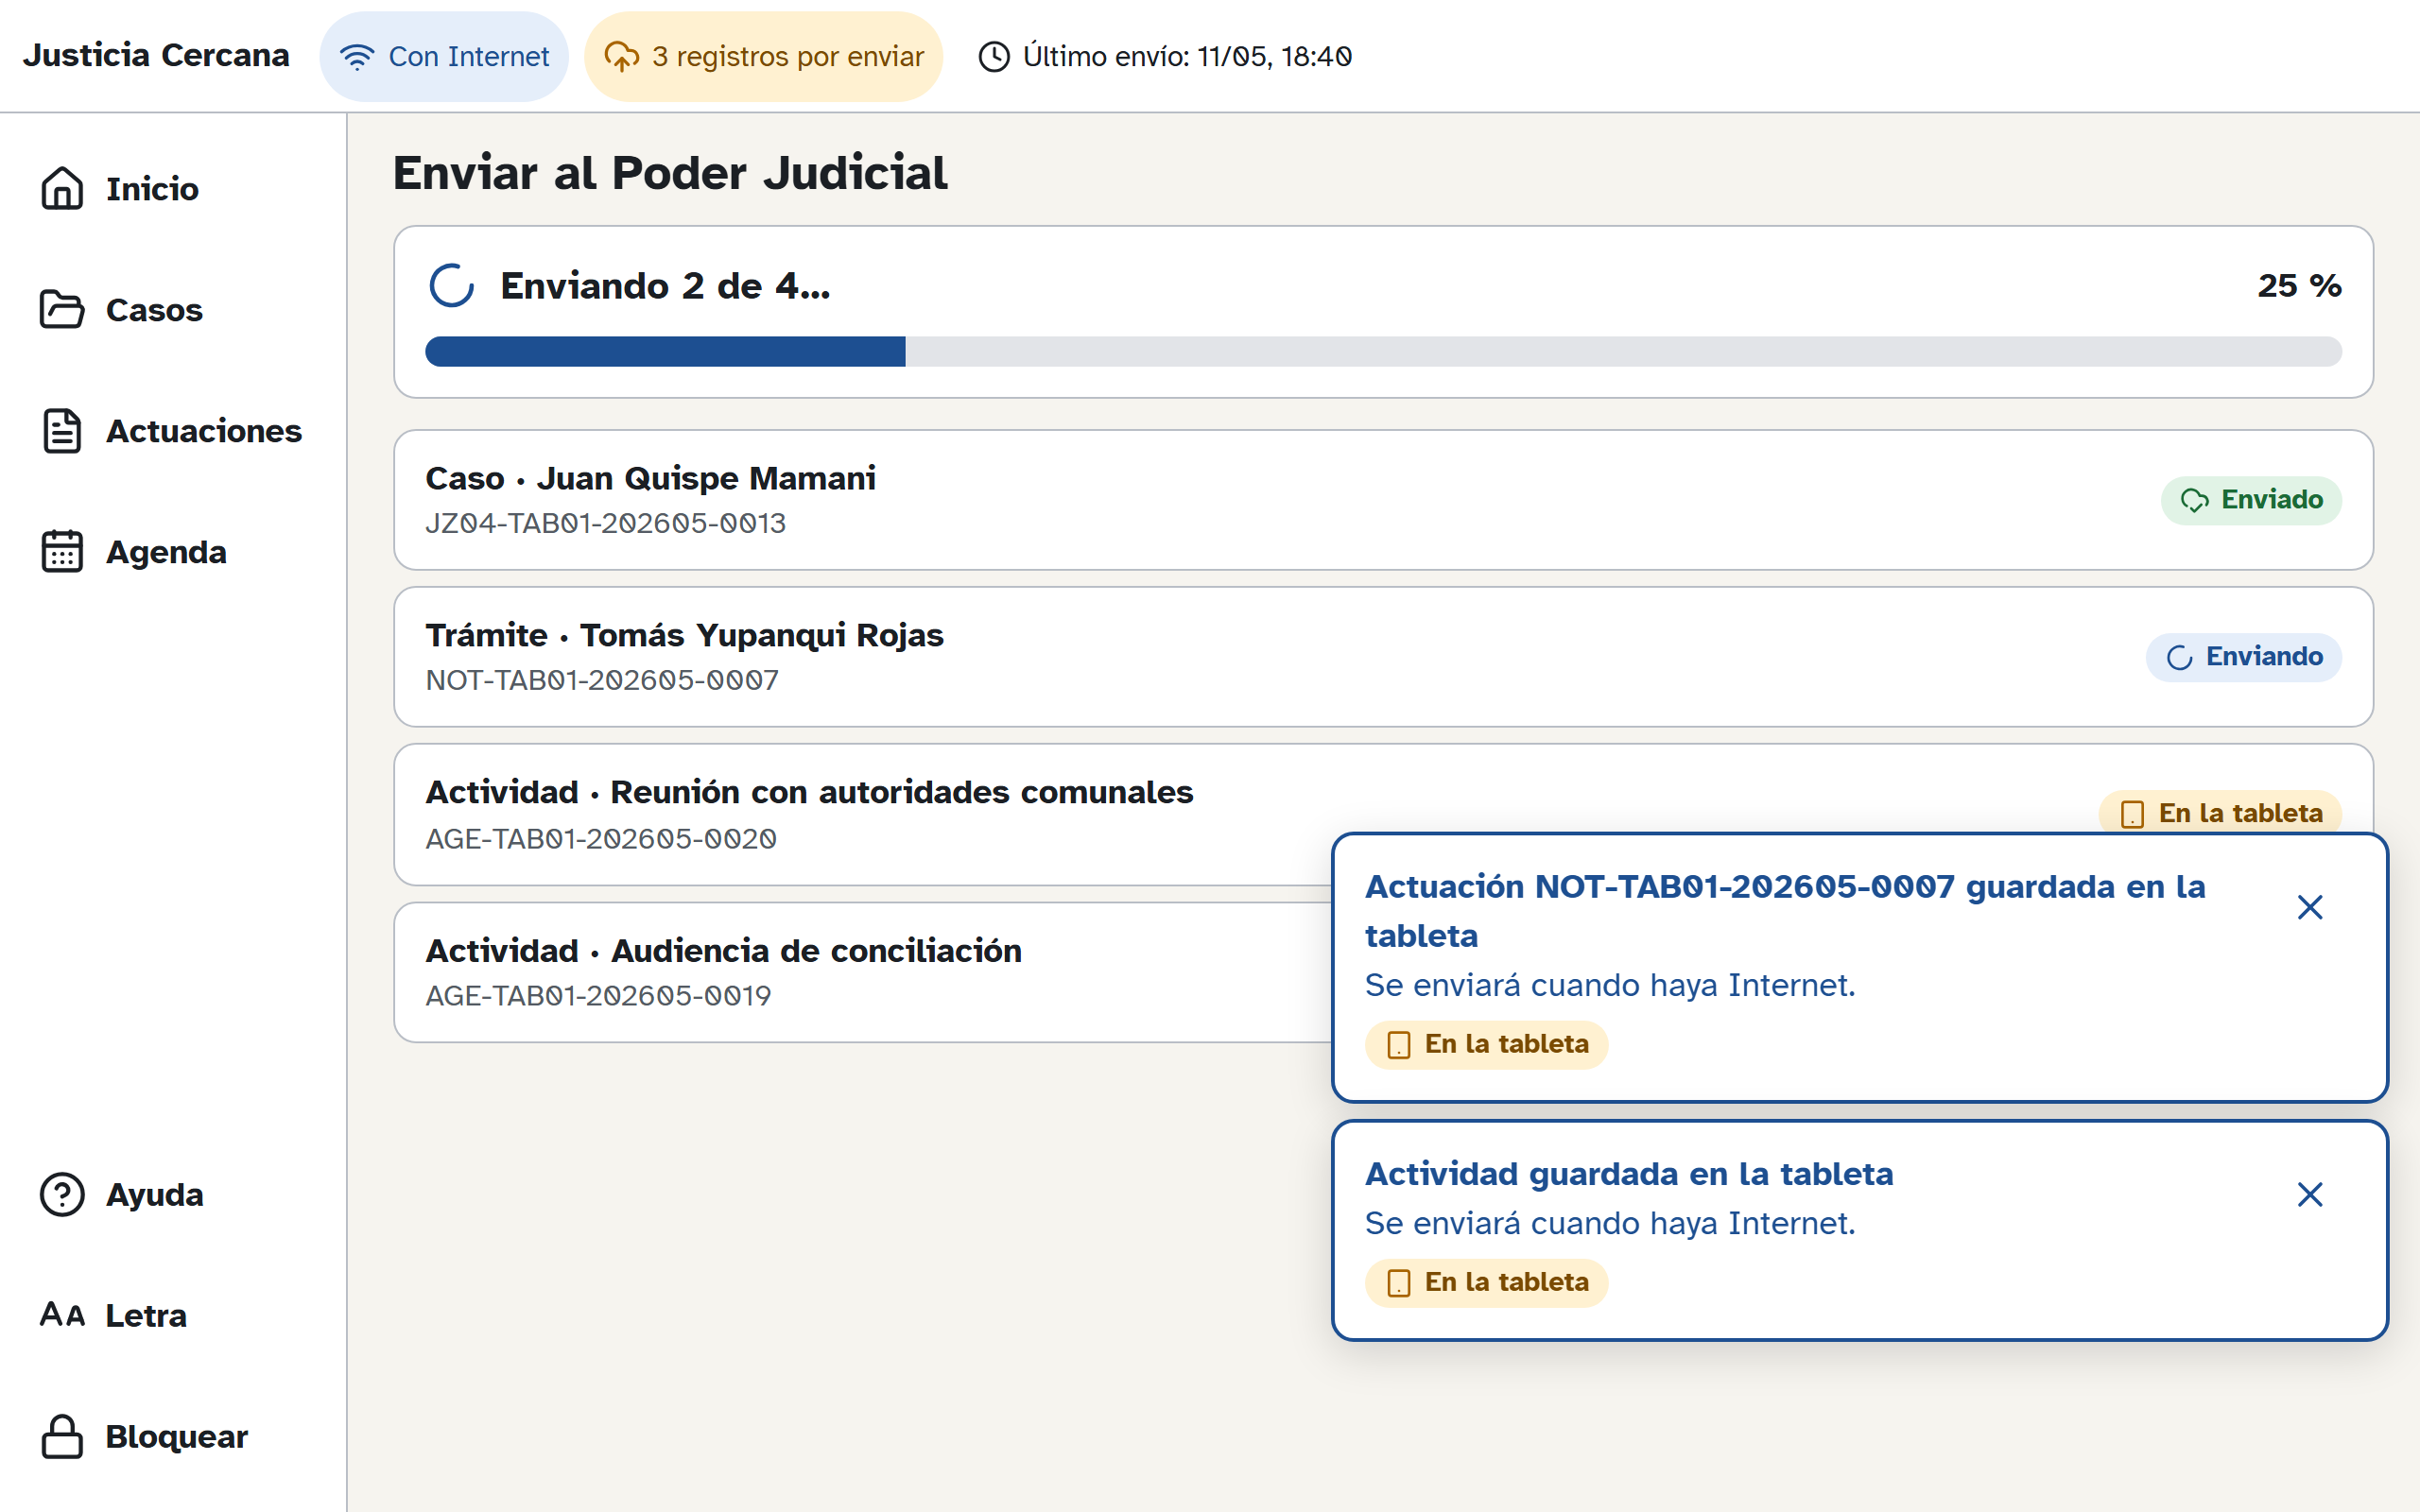
\includegraphics[width=\linewidth]{../../captures/F4-04_progreso-envio.png}\\[-2pt]{\footnotesize\raggedright\textbf{P-09 · 4.} Envío automático al volver el Internet con progreso ``Enviando n de 4…'' \emph{(Funcionamiento sin conexión)}\par}\end{minipage}\hfill
\begin{minipage}[t]{0.49\textwidth}\centering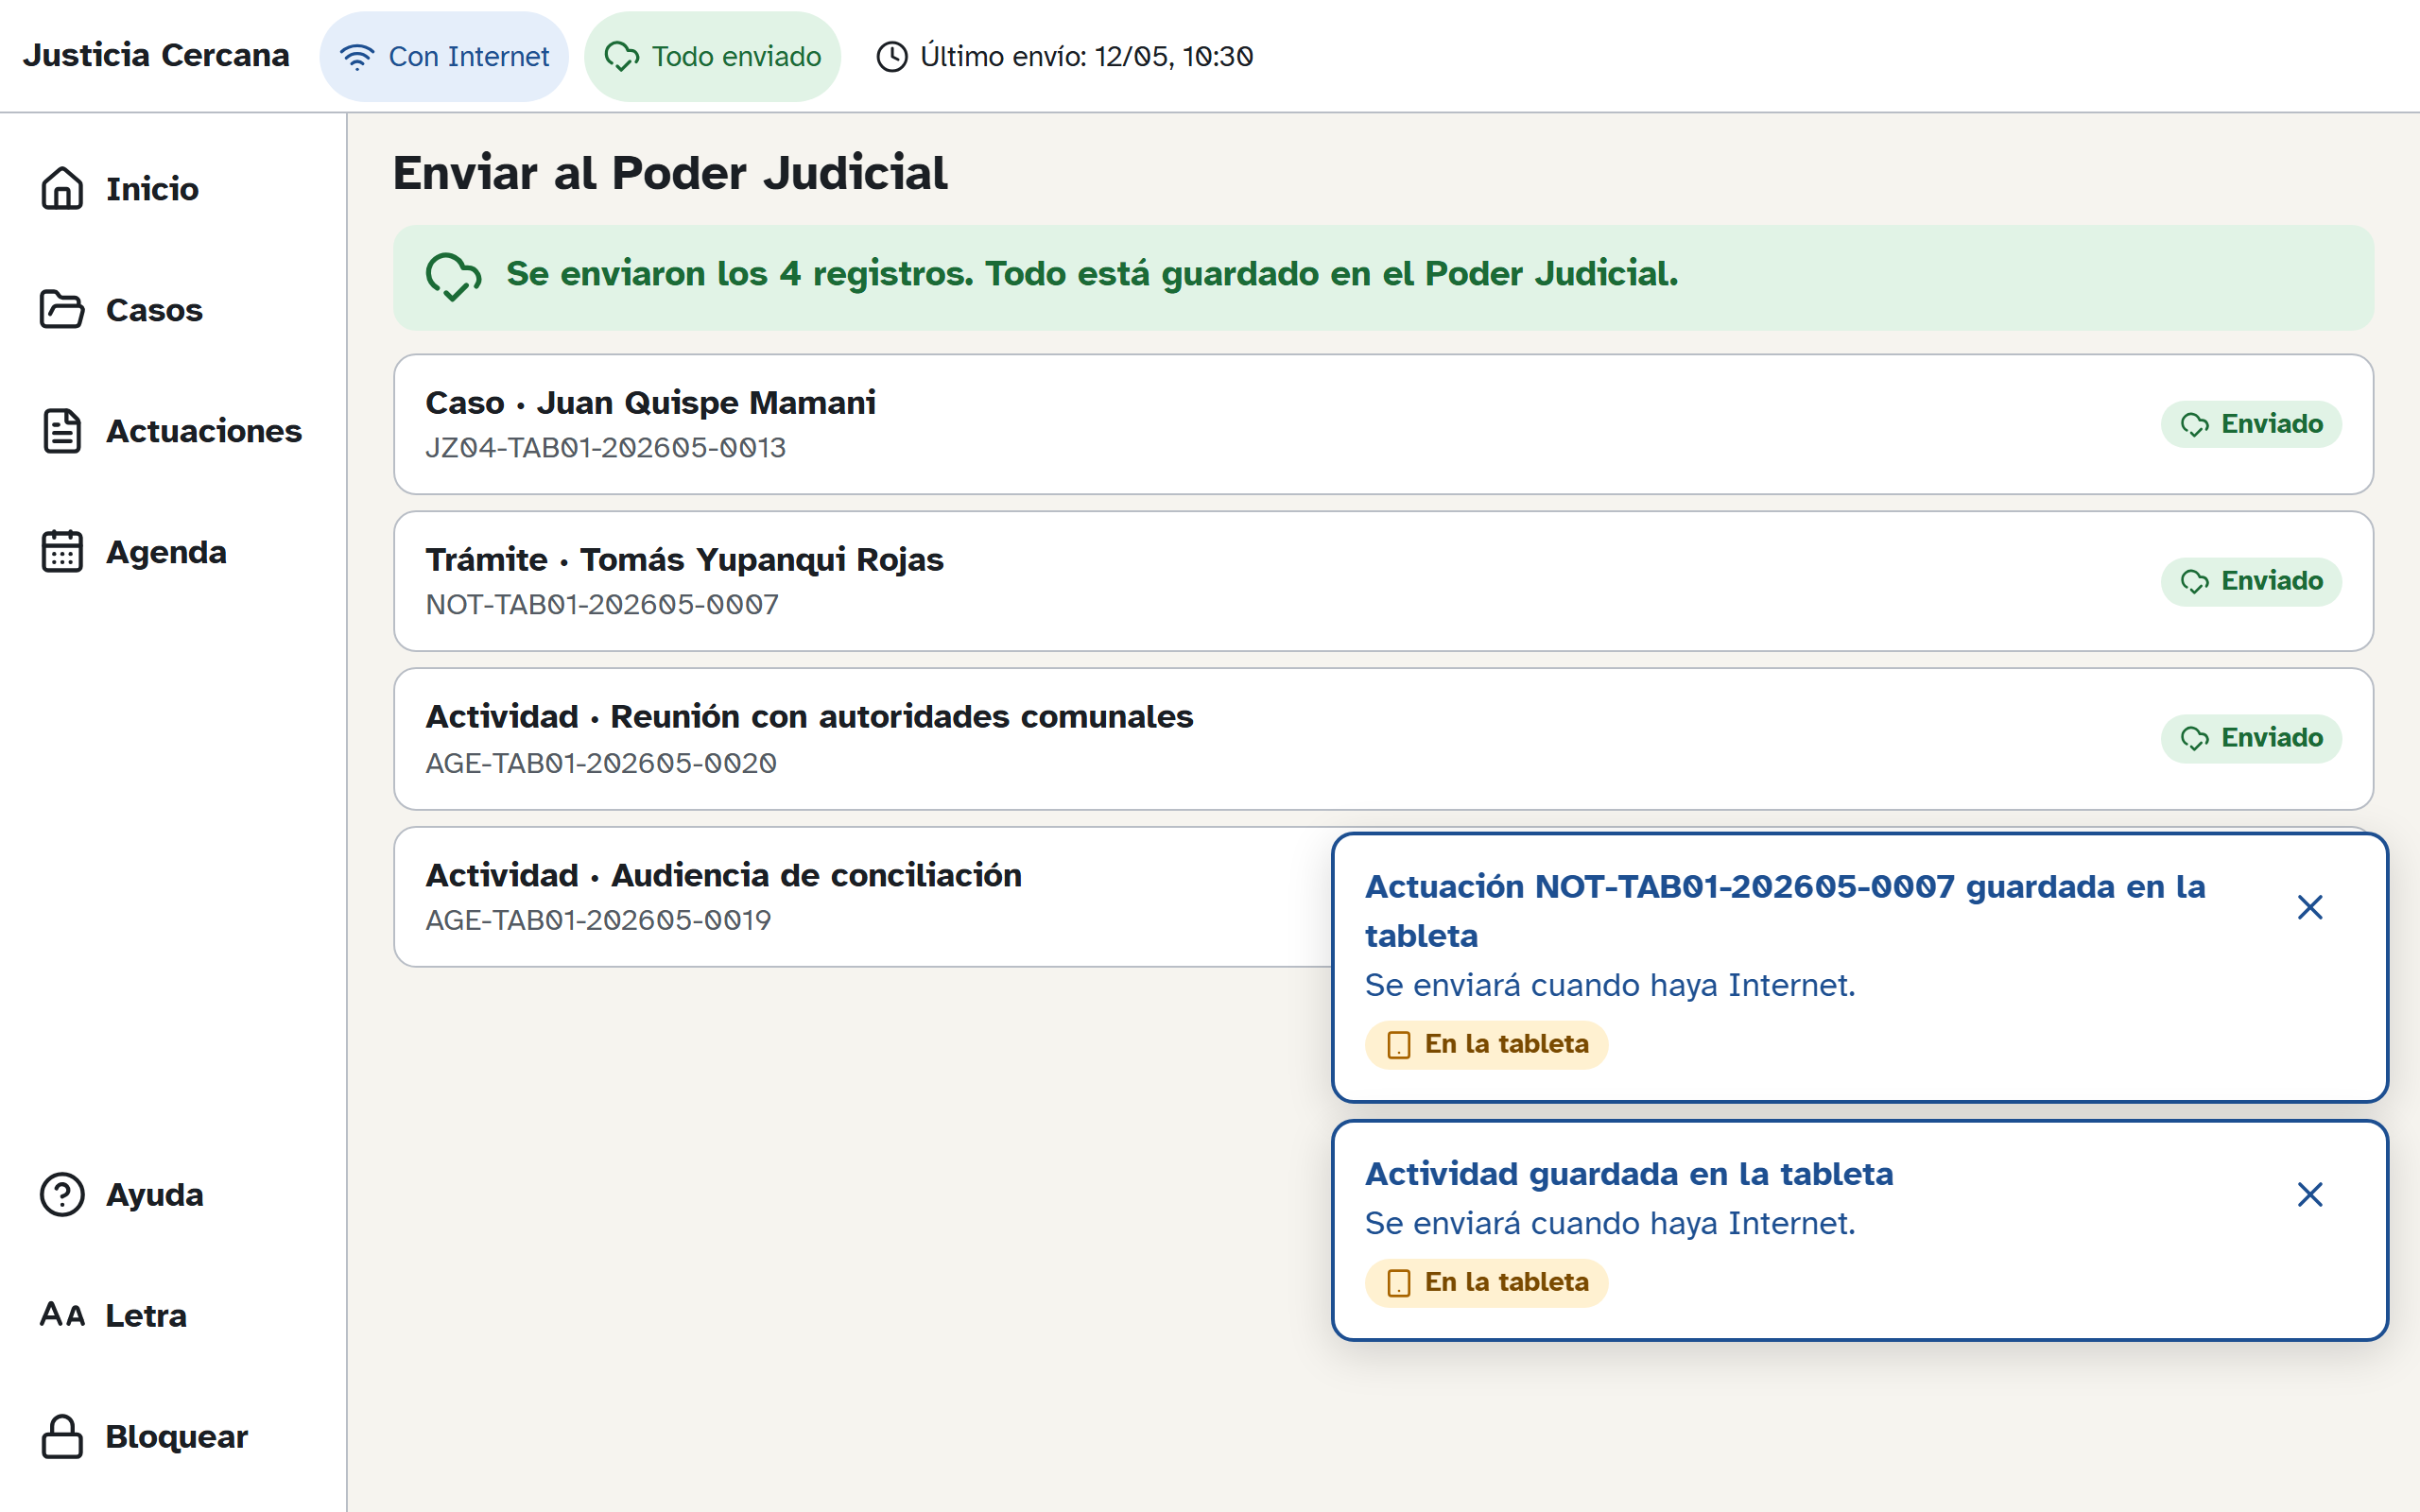
\includegraphics[width=\linewidth]{../../captures/F4-05a_exito-todo-enviado.png}\\[-2pt]{\footnotesize\raggedright\textbf{P-09 · 5.} ``Se enviaron los 4 registros'' y barra ``Todo enviado''; distintivos ``Enviado'' \emph{(Funcionamiento sin conexión)}\par}\end{minipage}\par\vspace{8pt}\noindent
\begin{minipage}[t]{0.49\textwidth}\centering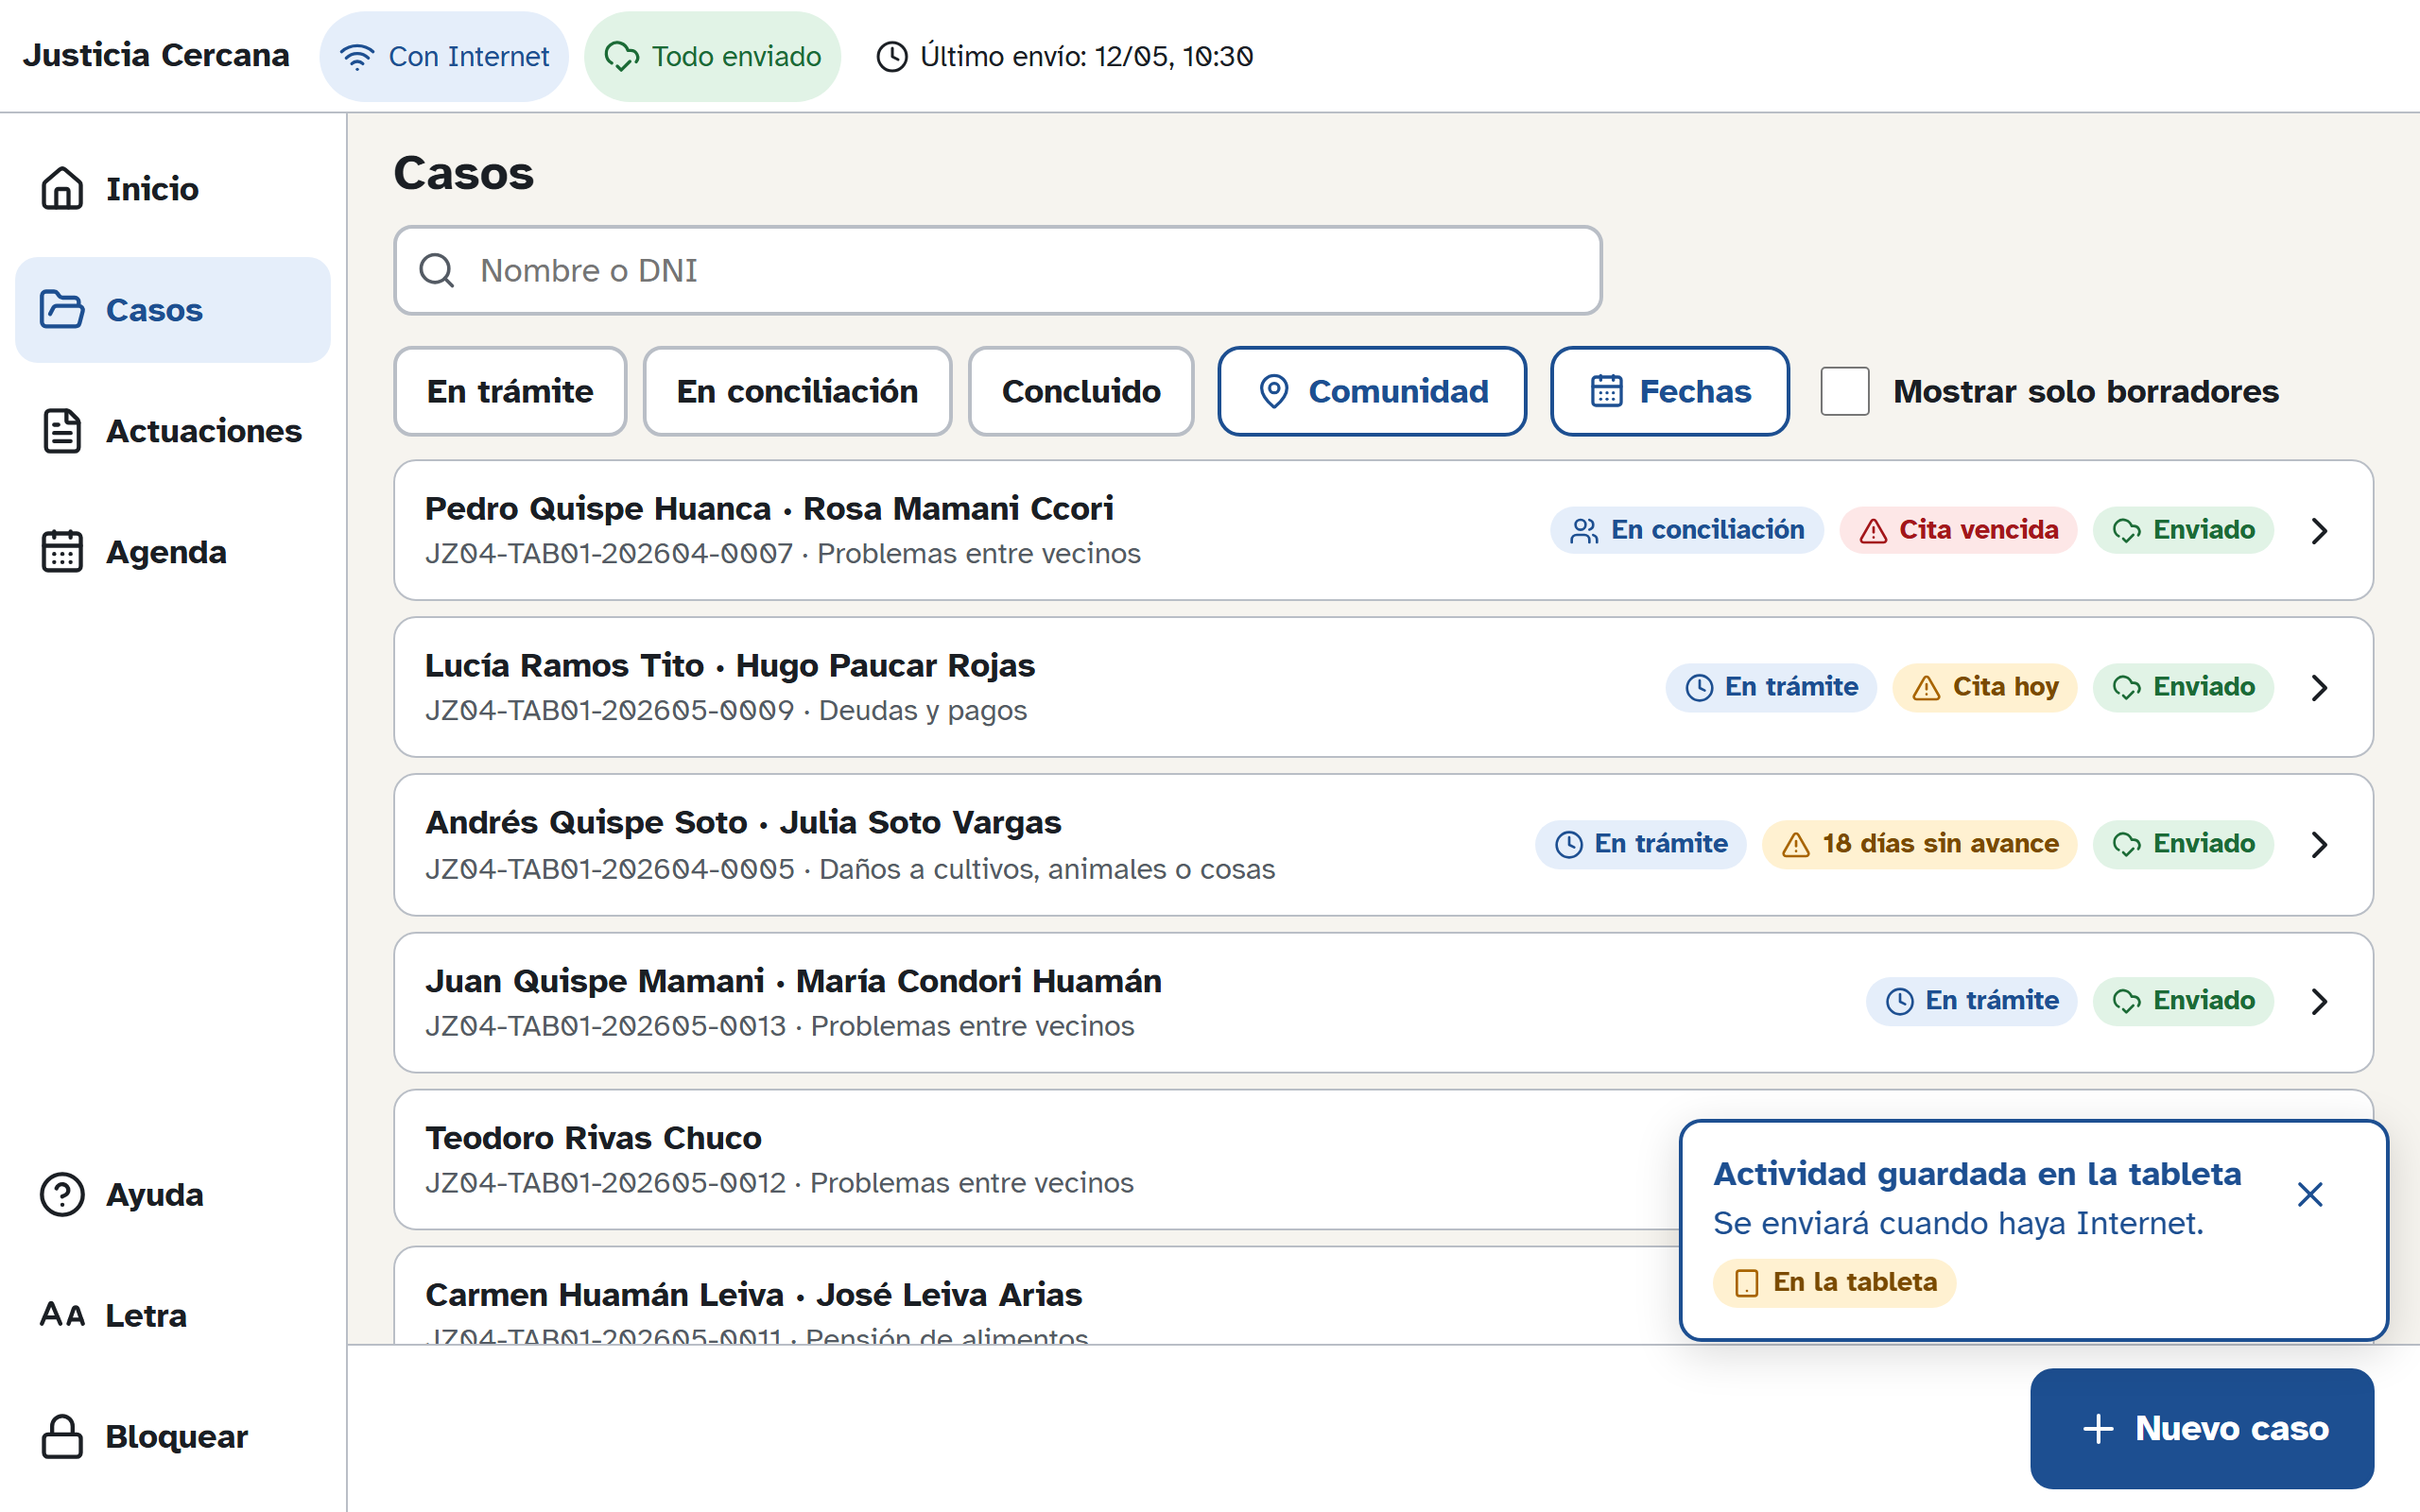
\includegraphics[width=\linewidth]{../../captures/F4-05b_distintivos-enviado.png}\\[-2pt]{\footnotesize\raggedright\textbf{P-02 · 5.} El caso del Flujo 1 pasa a ``Enviado'' en la lista \emph{(Funcionamiento sin conexión)}\par}\end{minipage}\hfill
\begin{minipage}[t]{0.49\textwidth}\centering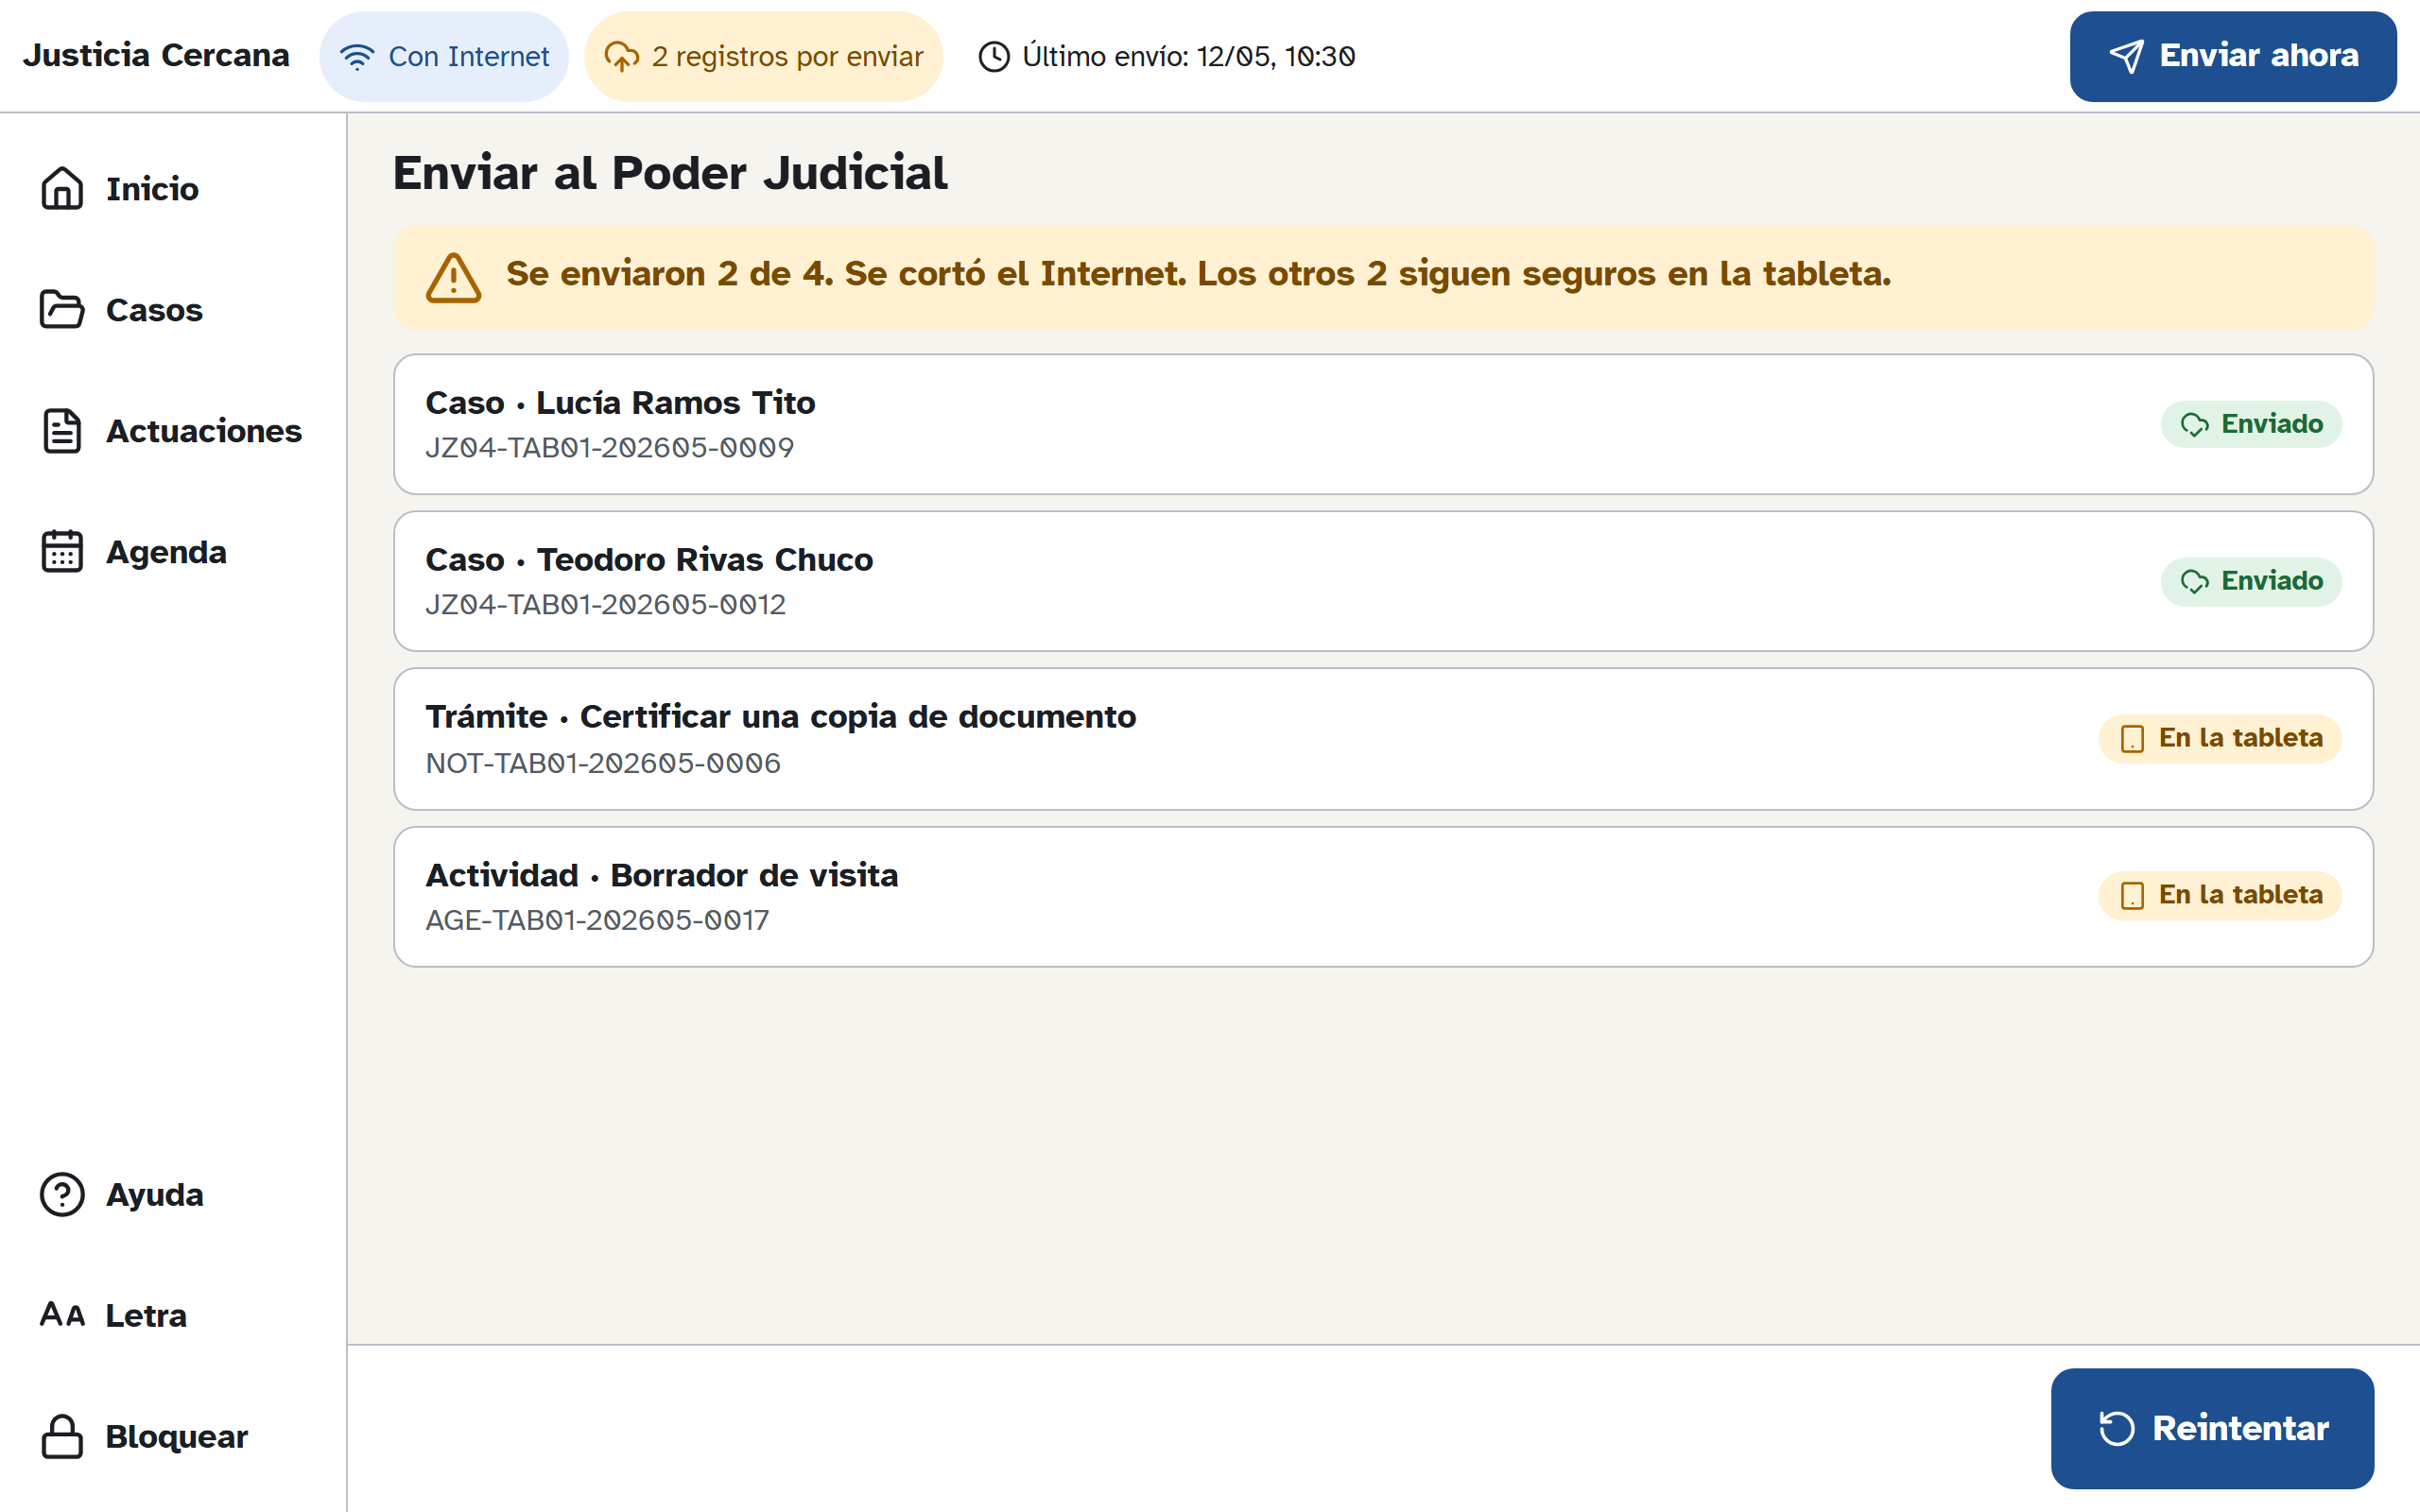
\includegraphics[width=\linewidth]{../../captures/F4-06a_fallo-parcial.png}\\[-2pt]{\footnotesize\raggedright\textbf{P-09 · 6.} Fallo parcial: ``Se enviaron 2 de 4…'' con [Reintentar] \emph{(Funcionamiento sin conexión)}\par}\end{minipage}\par\vspace{8pt}\noindent
\begin{minipage}[t]{0.49\textwidth}\centering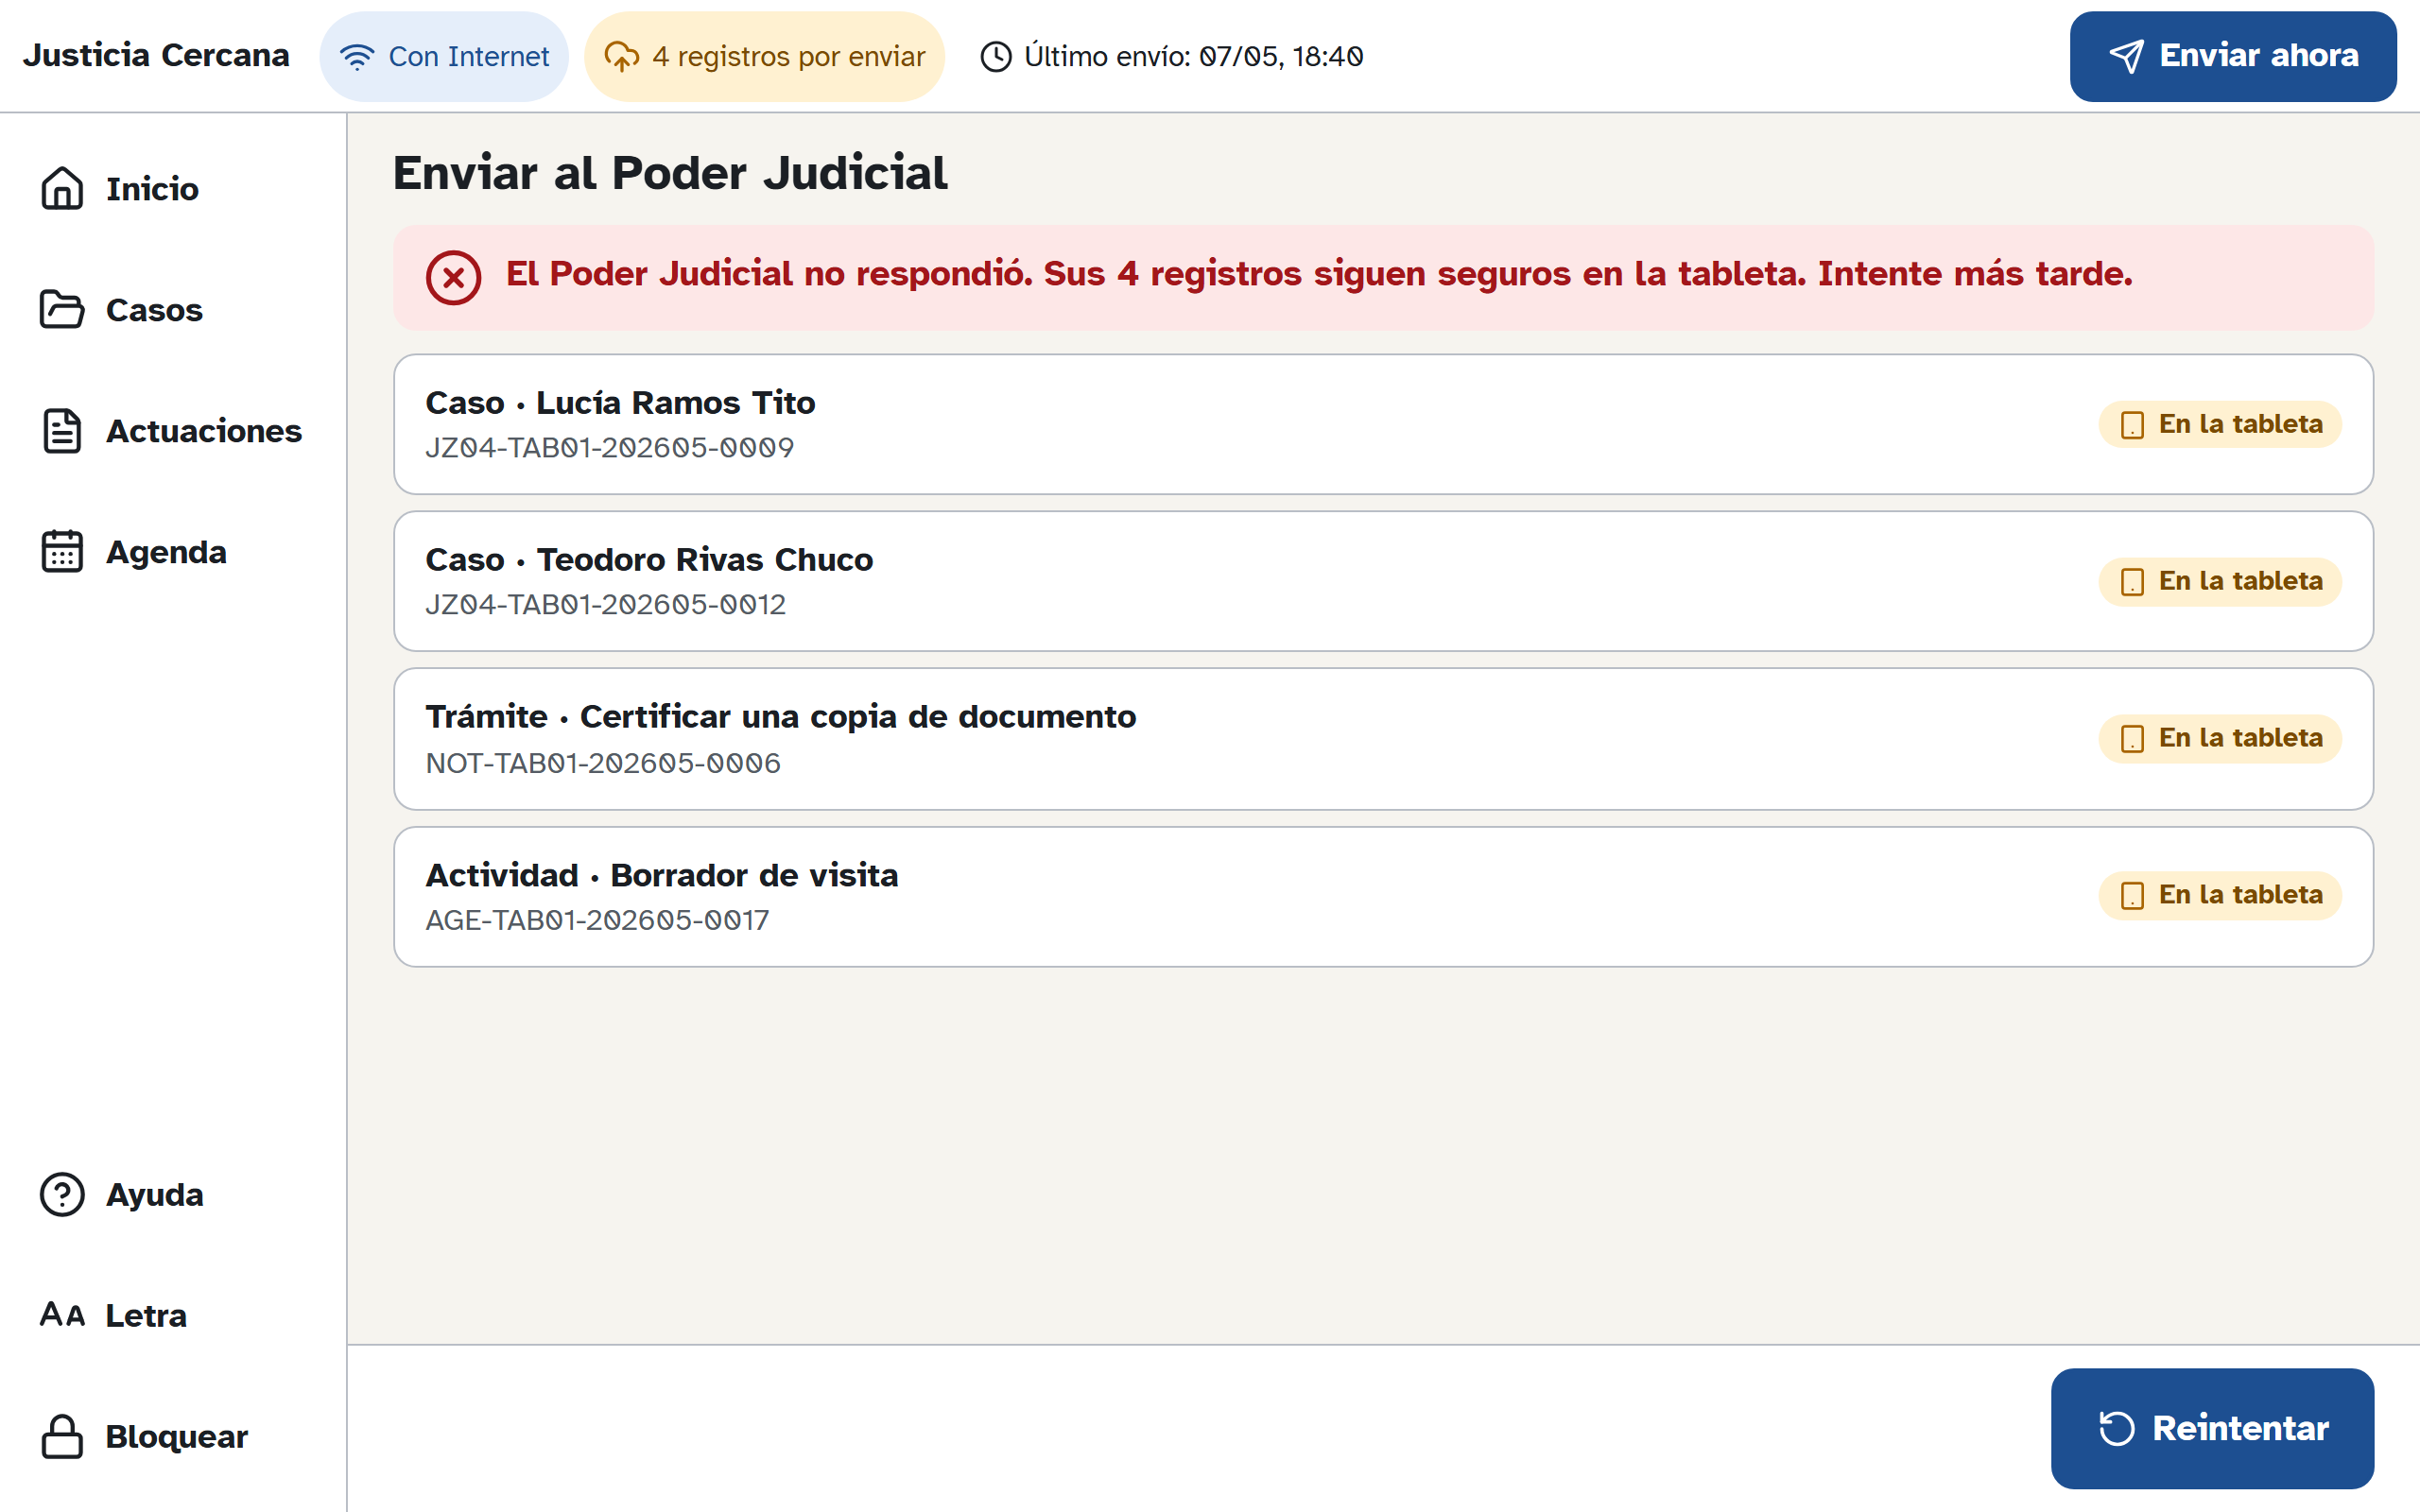
\includegraphics[width=\linewidth]{../../captures/F4-06b_error-servidor.png}\\[-2pt]{\footnotesize\raggedright\textbf{P-09 · 6.} Error del servidor: registros seguros en la tableta, [Reintentar] \emph{(Funcionamiento sin conexión)}\par}\end{minipage}\hfill
\begin{minipage}[t]{0.49\textwidth}\centering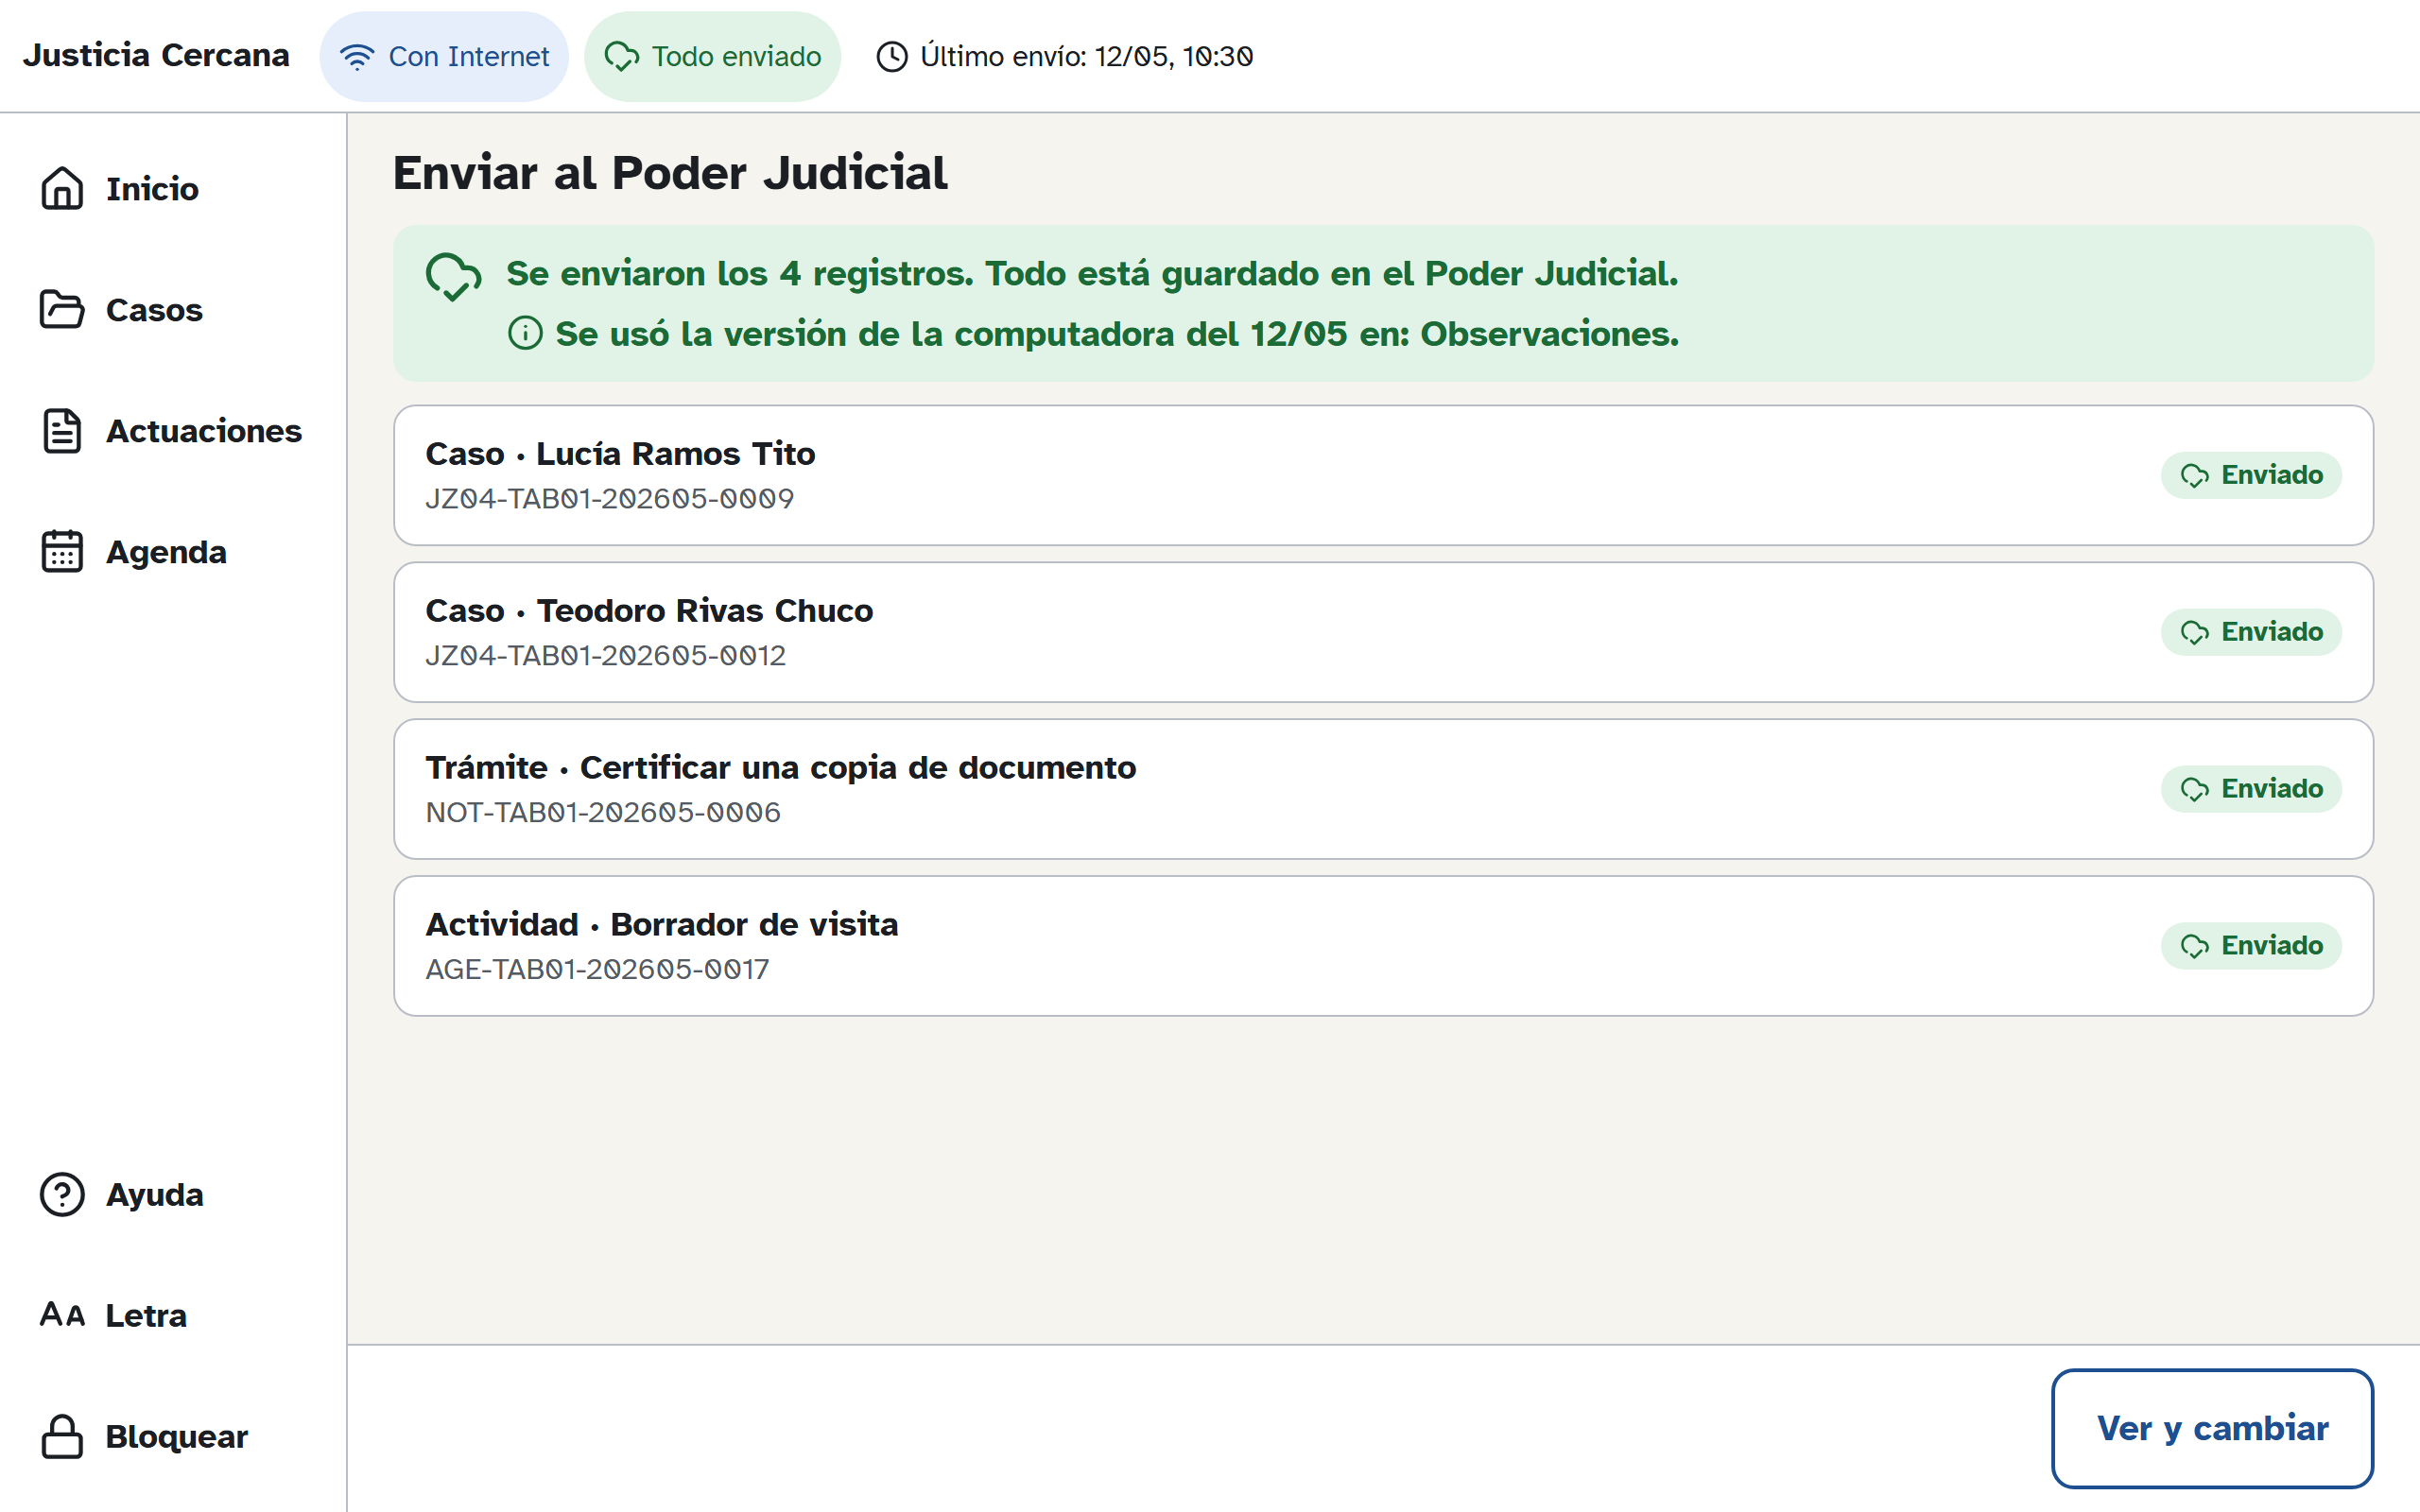
\includegraphics[width=\linewidth]{../../captures/F4-06c_conflicto-resuelto.png}\\[-2pt]{\footnotesize\raggedright\textbf{P-09 · 6.} Conflicto resuelto automáticamente con el cambio más reciente y aviso del campo \emph{(Funcionamiento sin conexión)}\par}\end{minipage}\par\vspace{8pt}\noindent
\begin{minipage}[t]{0.49\textwidth}\centering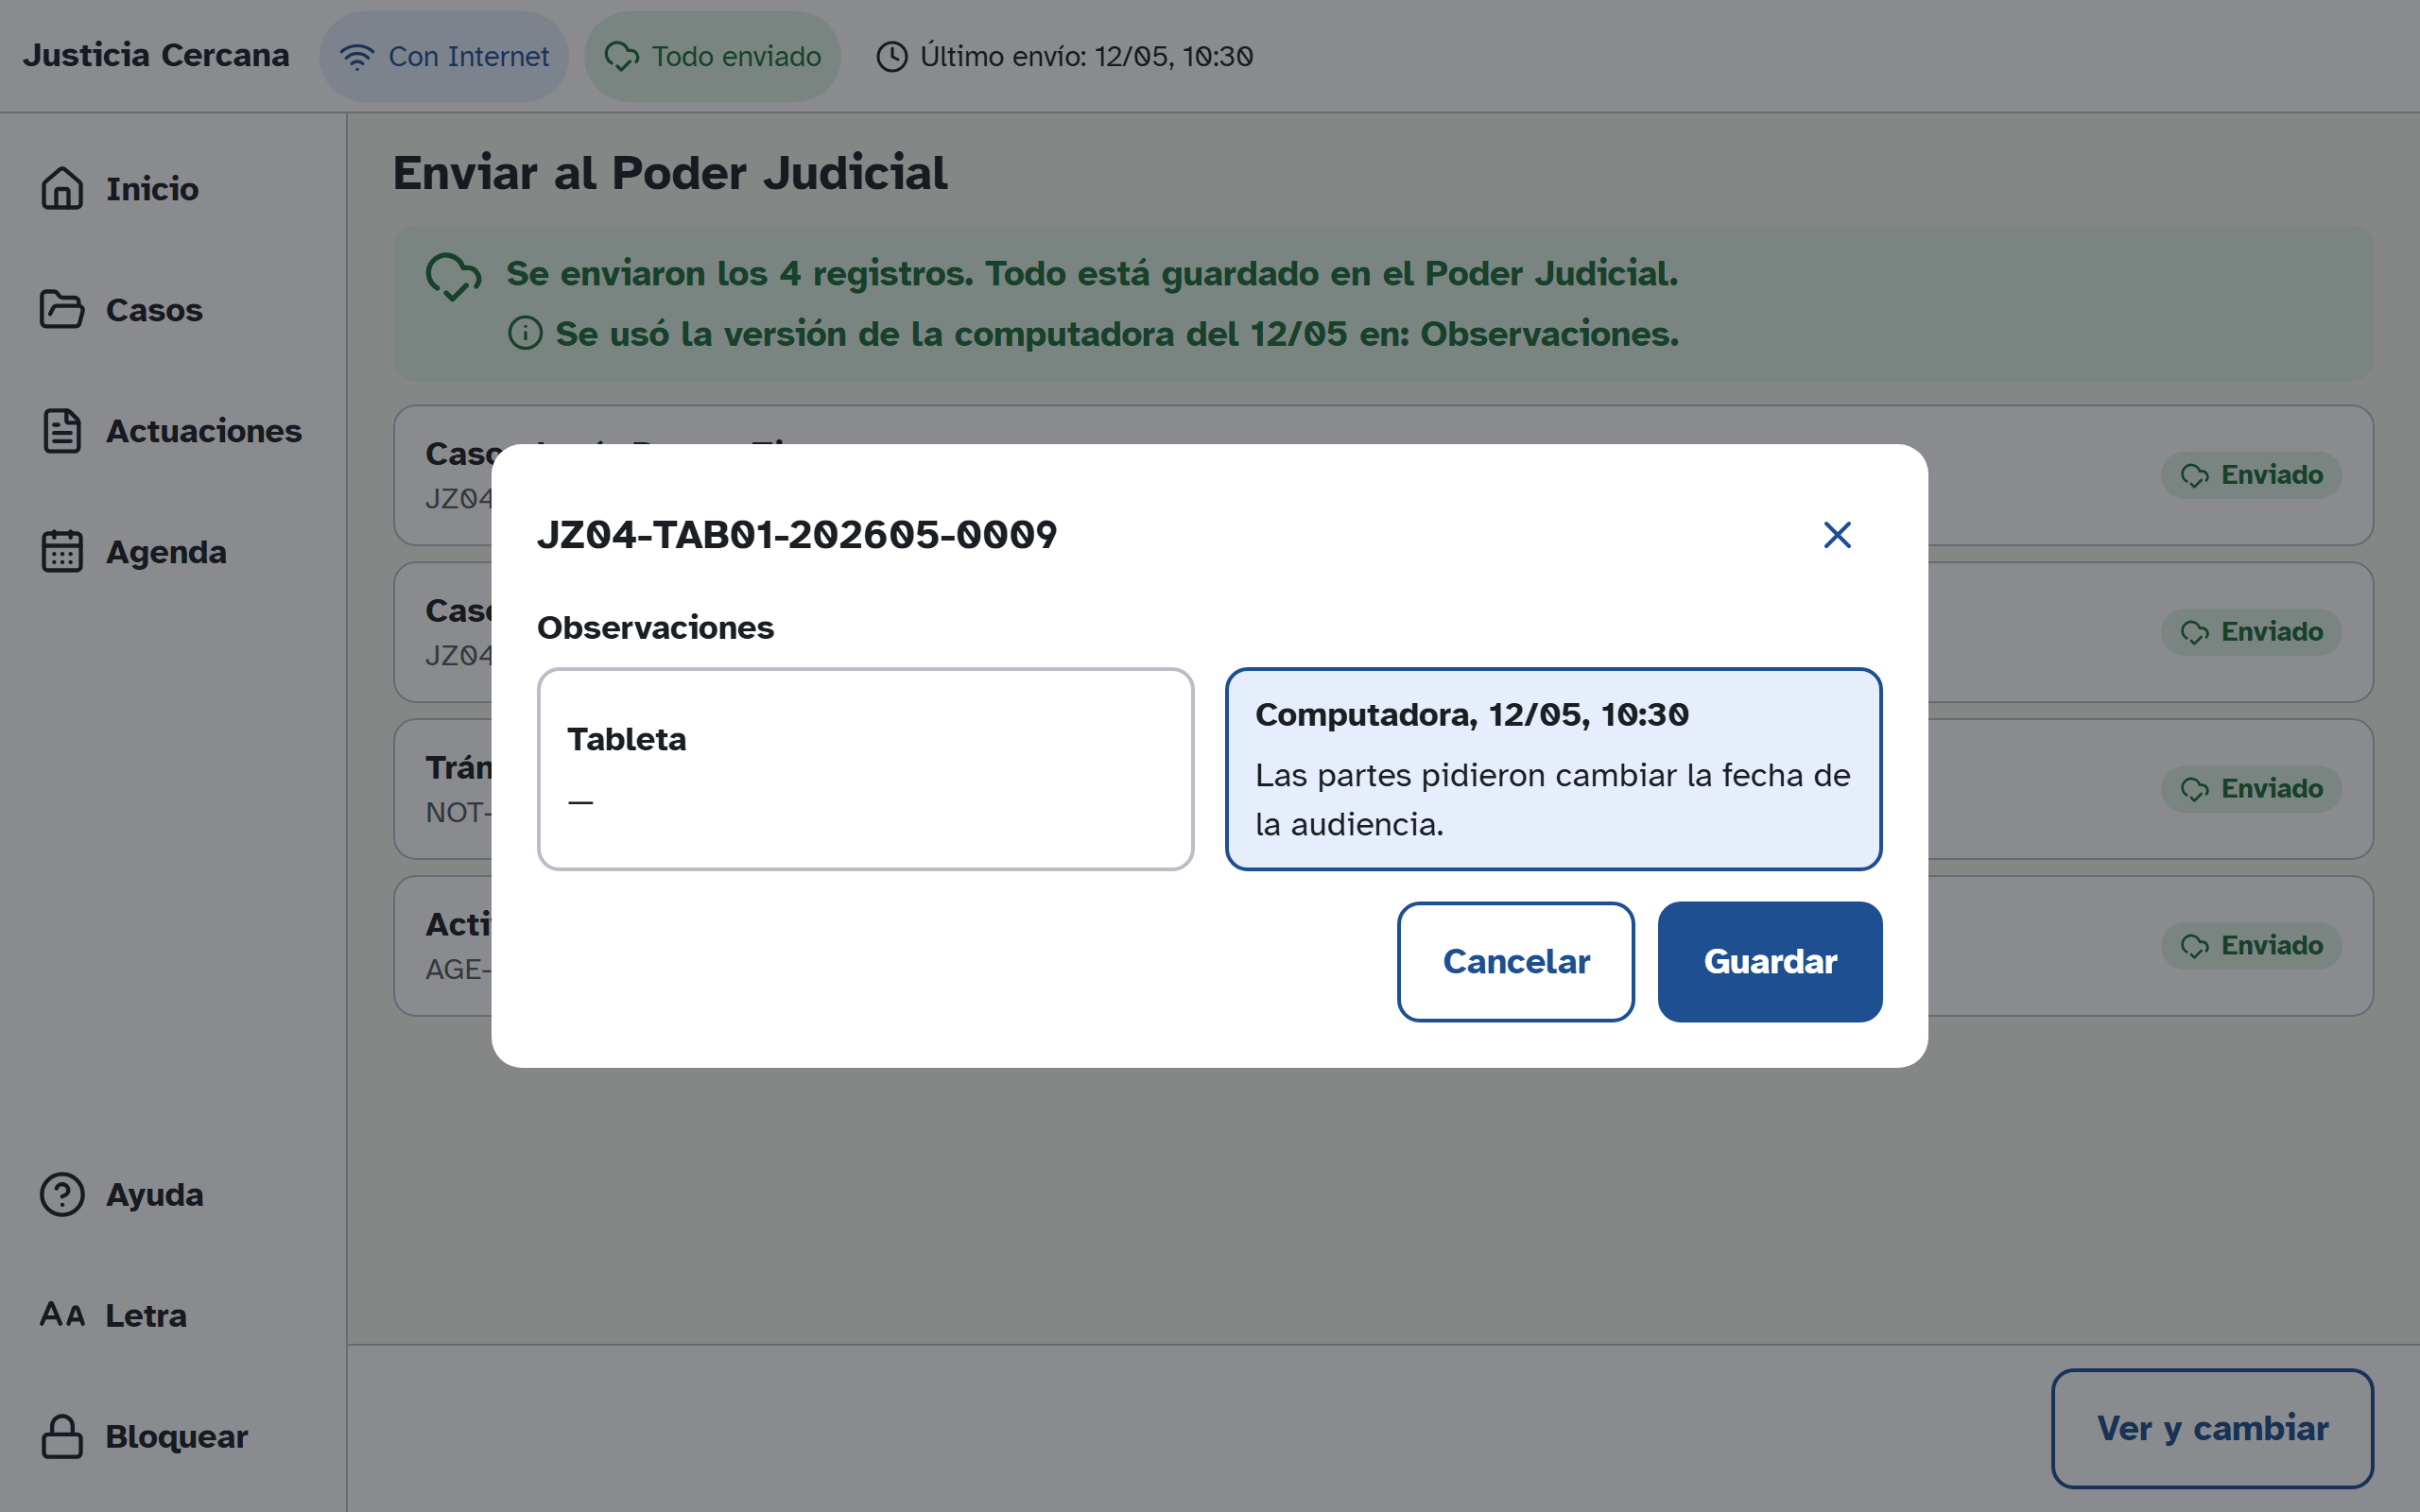
\includegraphics[width=\linewidth]{../../captures/F4-06d_ver-y-cambiar.png}\\[-2pt]{\footnotesize\raggedright\textbf{P-09 · 6.} [Ver y cambiar]: comparación por campo tableta / computadora \emph{(Funcionamiento sin conexión)}\par}\end{minipage}\hfill
\par\vspace{4pt}
\subsection*{Flujo A}
\noindent
\begin{minipage}[t]{0.49\textwidth}\centering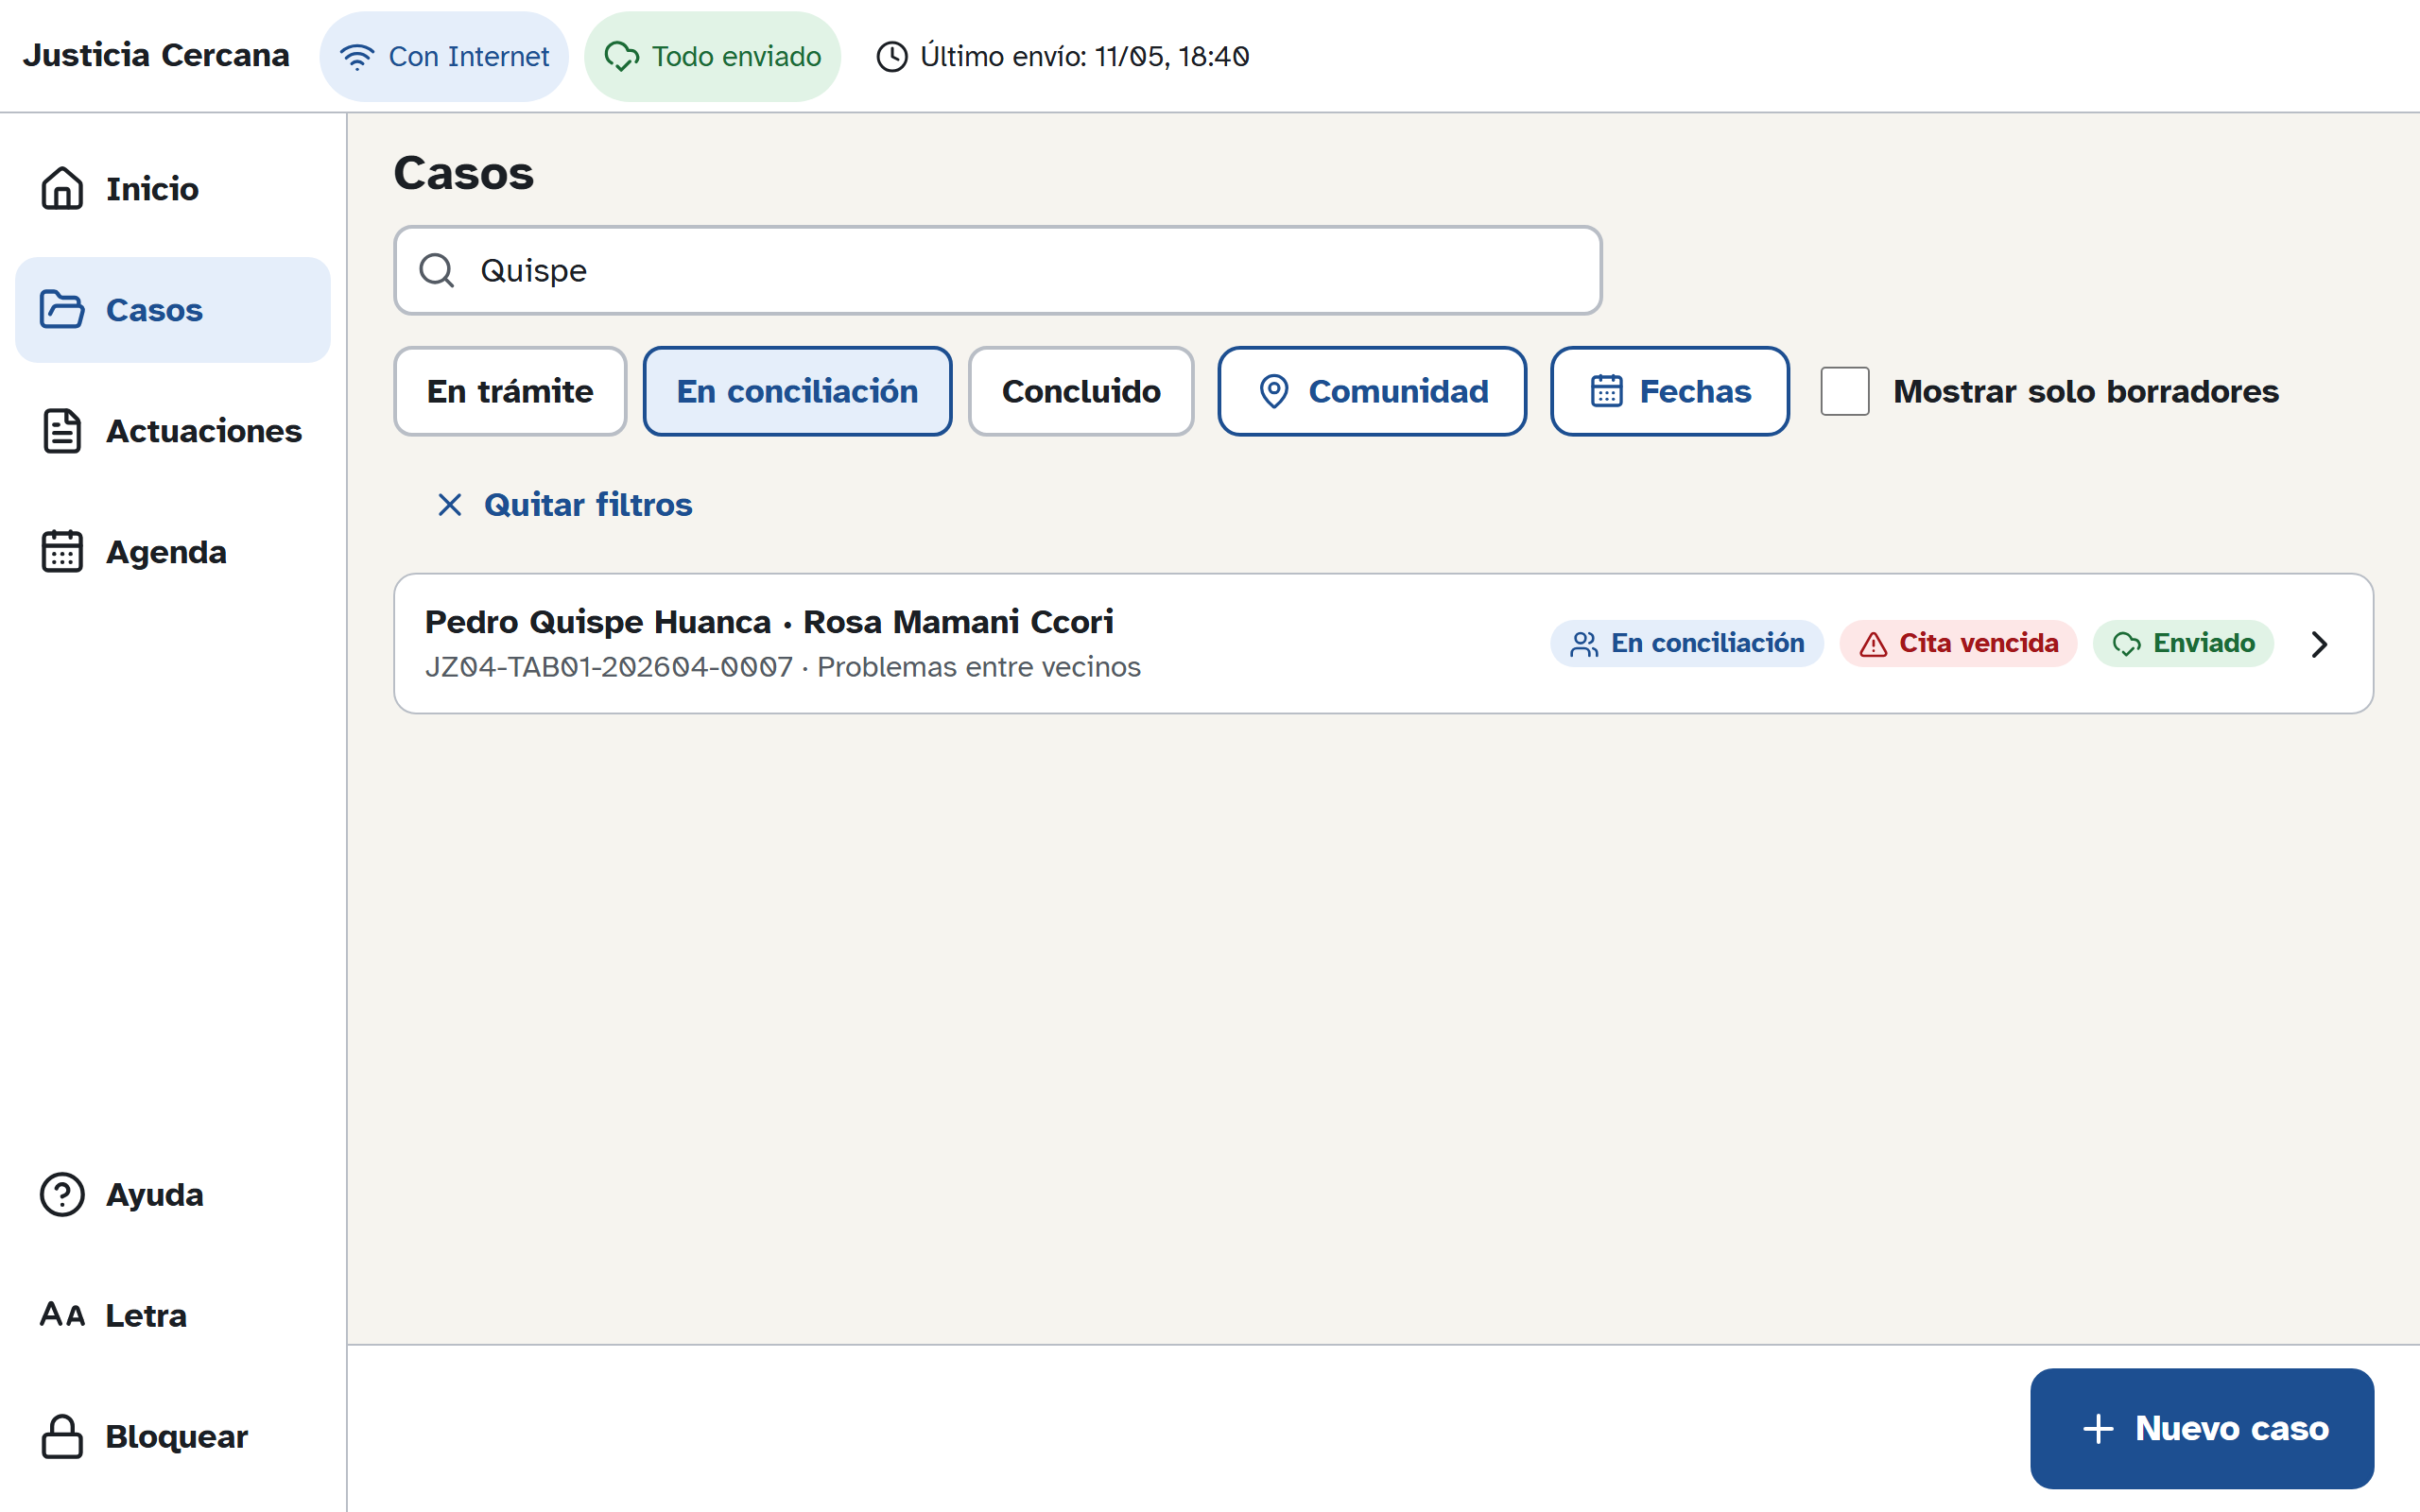
\includegraphics[width=\linewidth]{../../captures/FA-01_busqueda-filtro.png}\\[-2pt]{\footnotesize\raggedright\textbf{P-02 · 1.} Búsqueda ``Quispe'' + filtro En conciliación; motivo de atención en texto \emph{(Cobertura y funcionamiento de los módulos)}\par}\end{minipage}\hfill
\begin{minipage}[t]{0.49\textwidth}\centering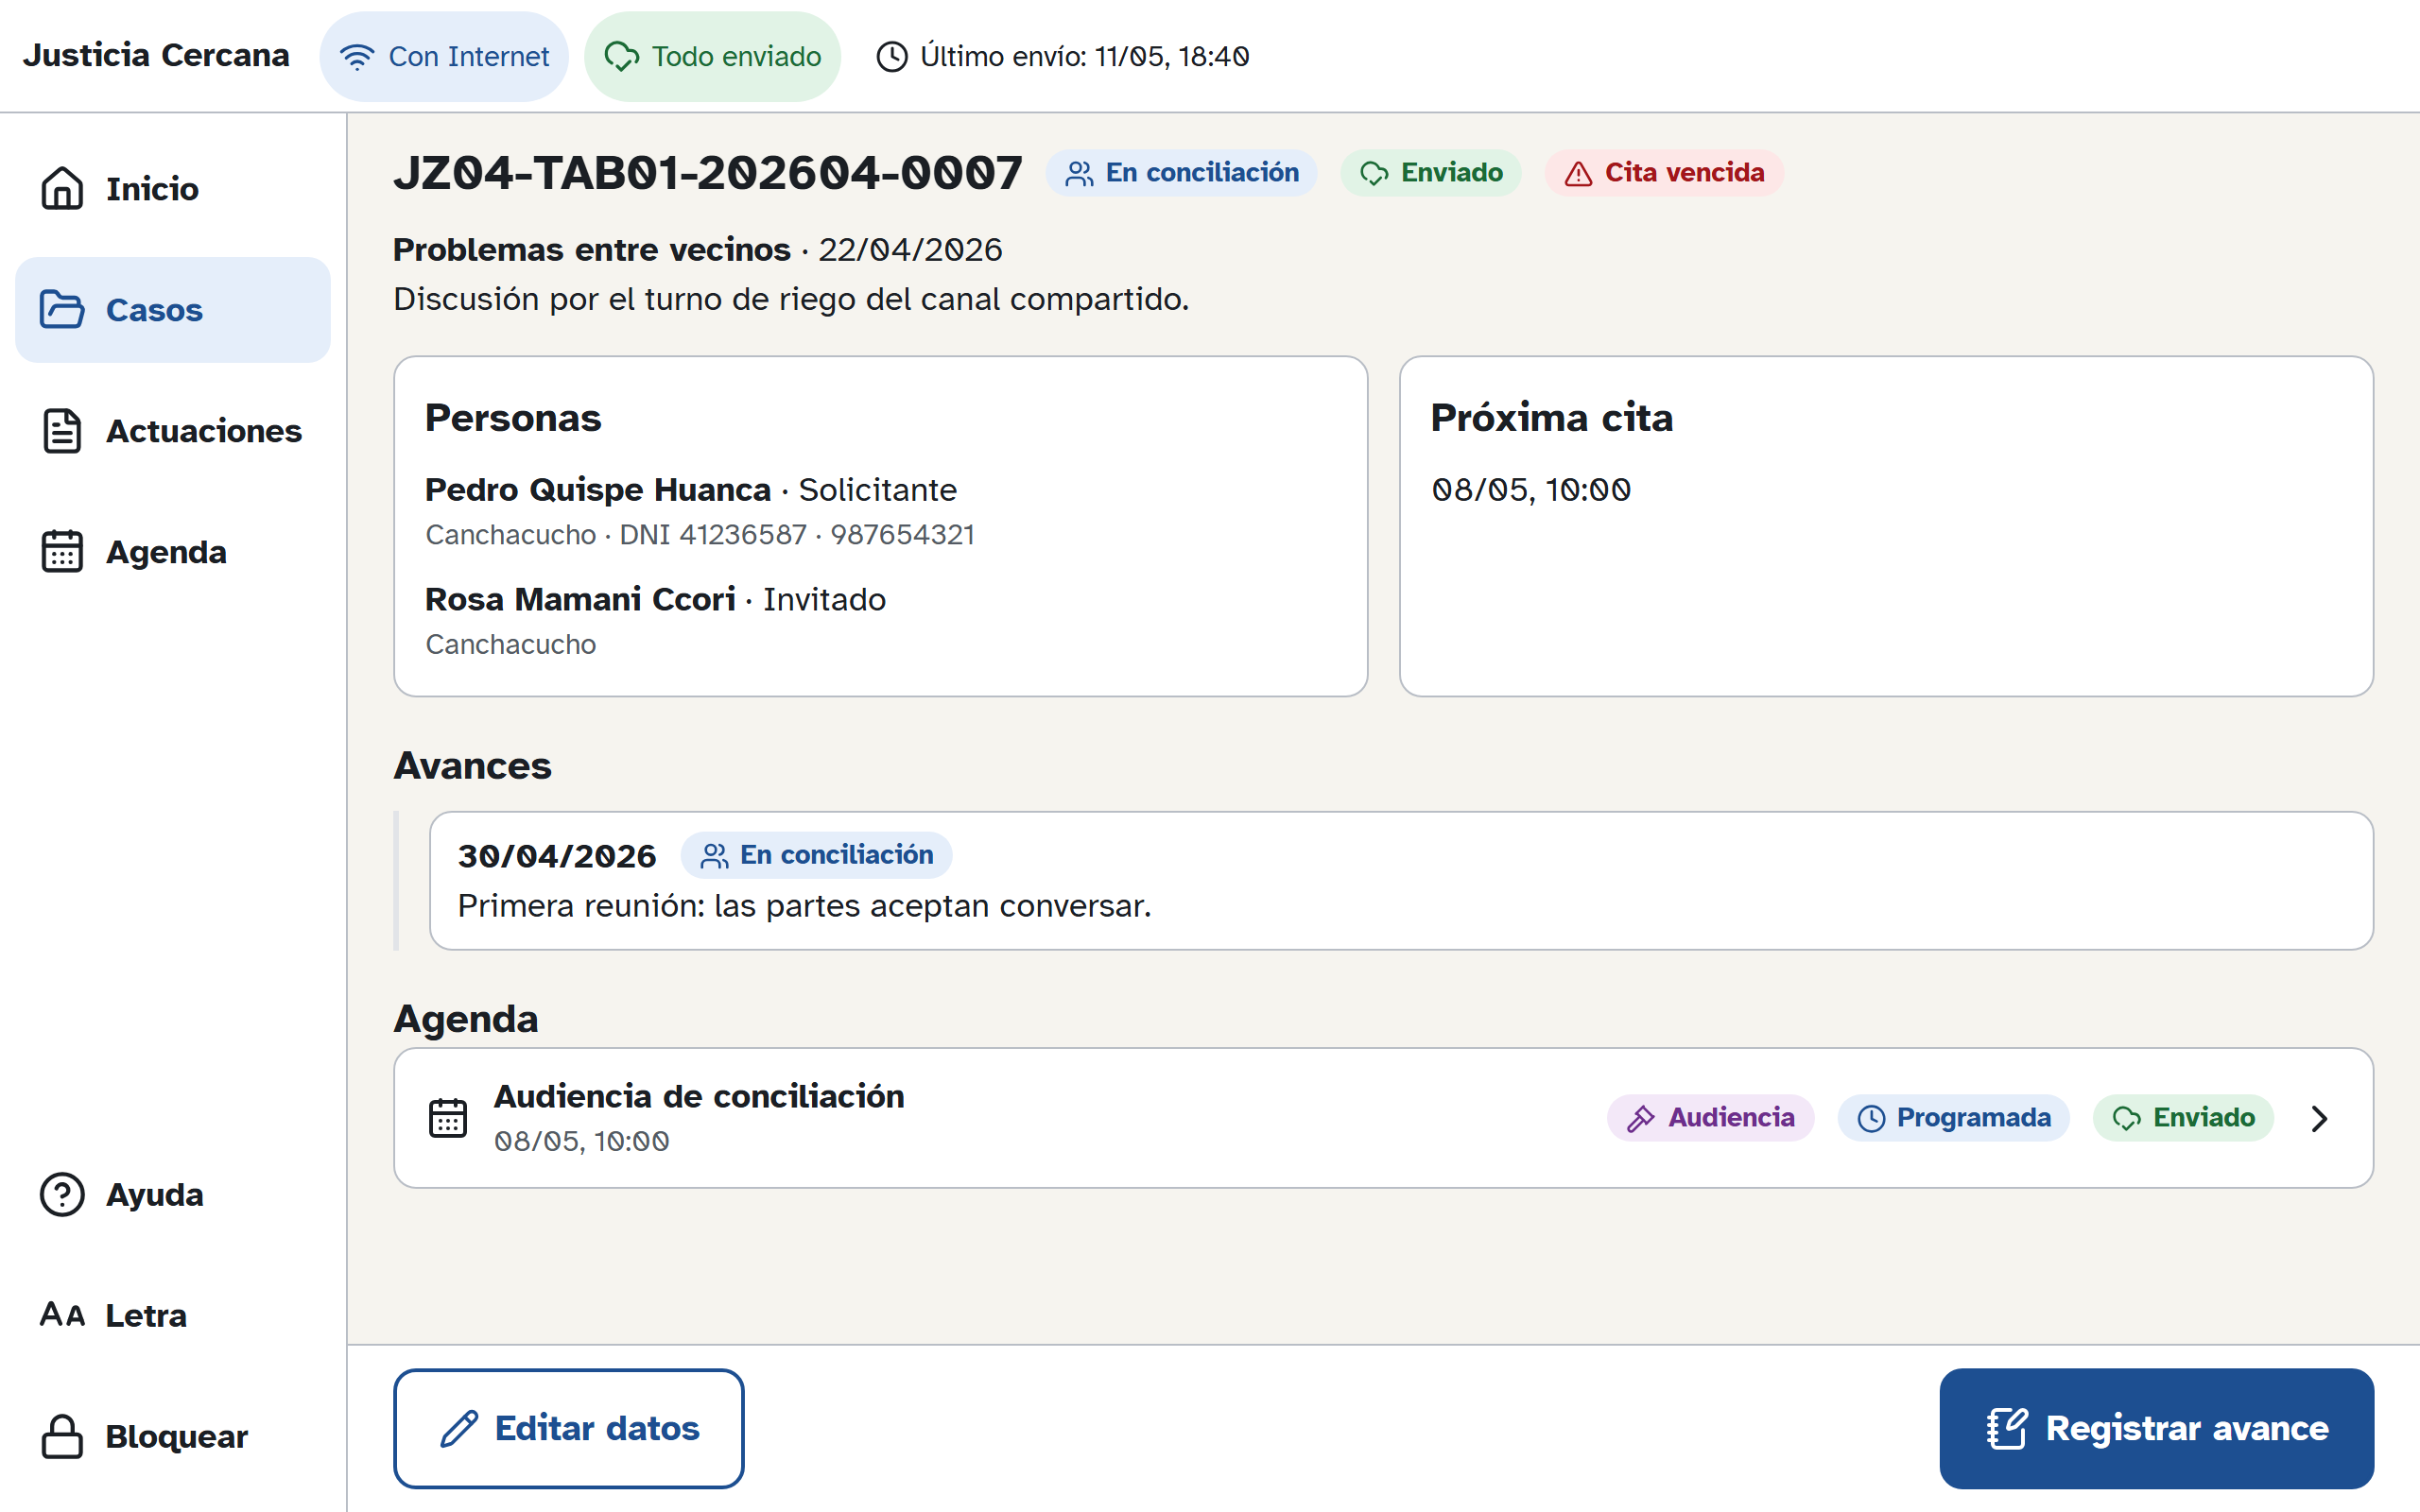
\includegraphics[width=\linewidth]{../../captures/FA-02_caso-cita-vencida.png}\\[-2pt]{\footnotesize\raggedright\textbf{P-04 · 2.} Detalle con ``Cita vencida'', distintivo, partes, historial \emph{(Cobertura y funcionamiento de los módulos)}\par}\end{minipage}\par\vspace{8pt}\noindent
\begin{minipage}[t]{0.49\textwidth}\centering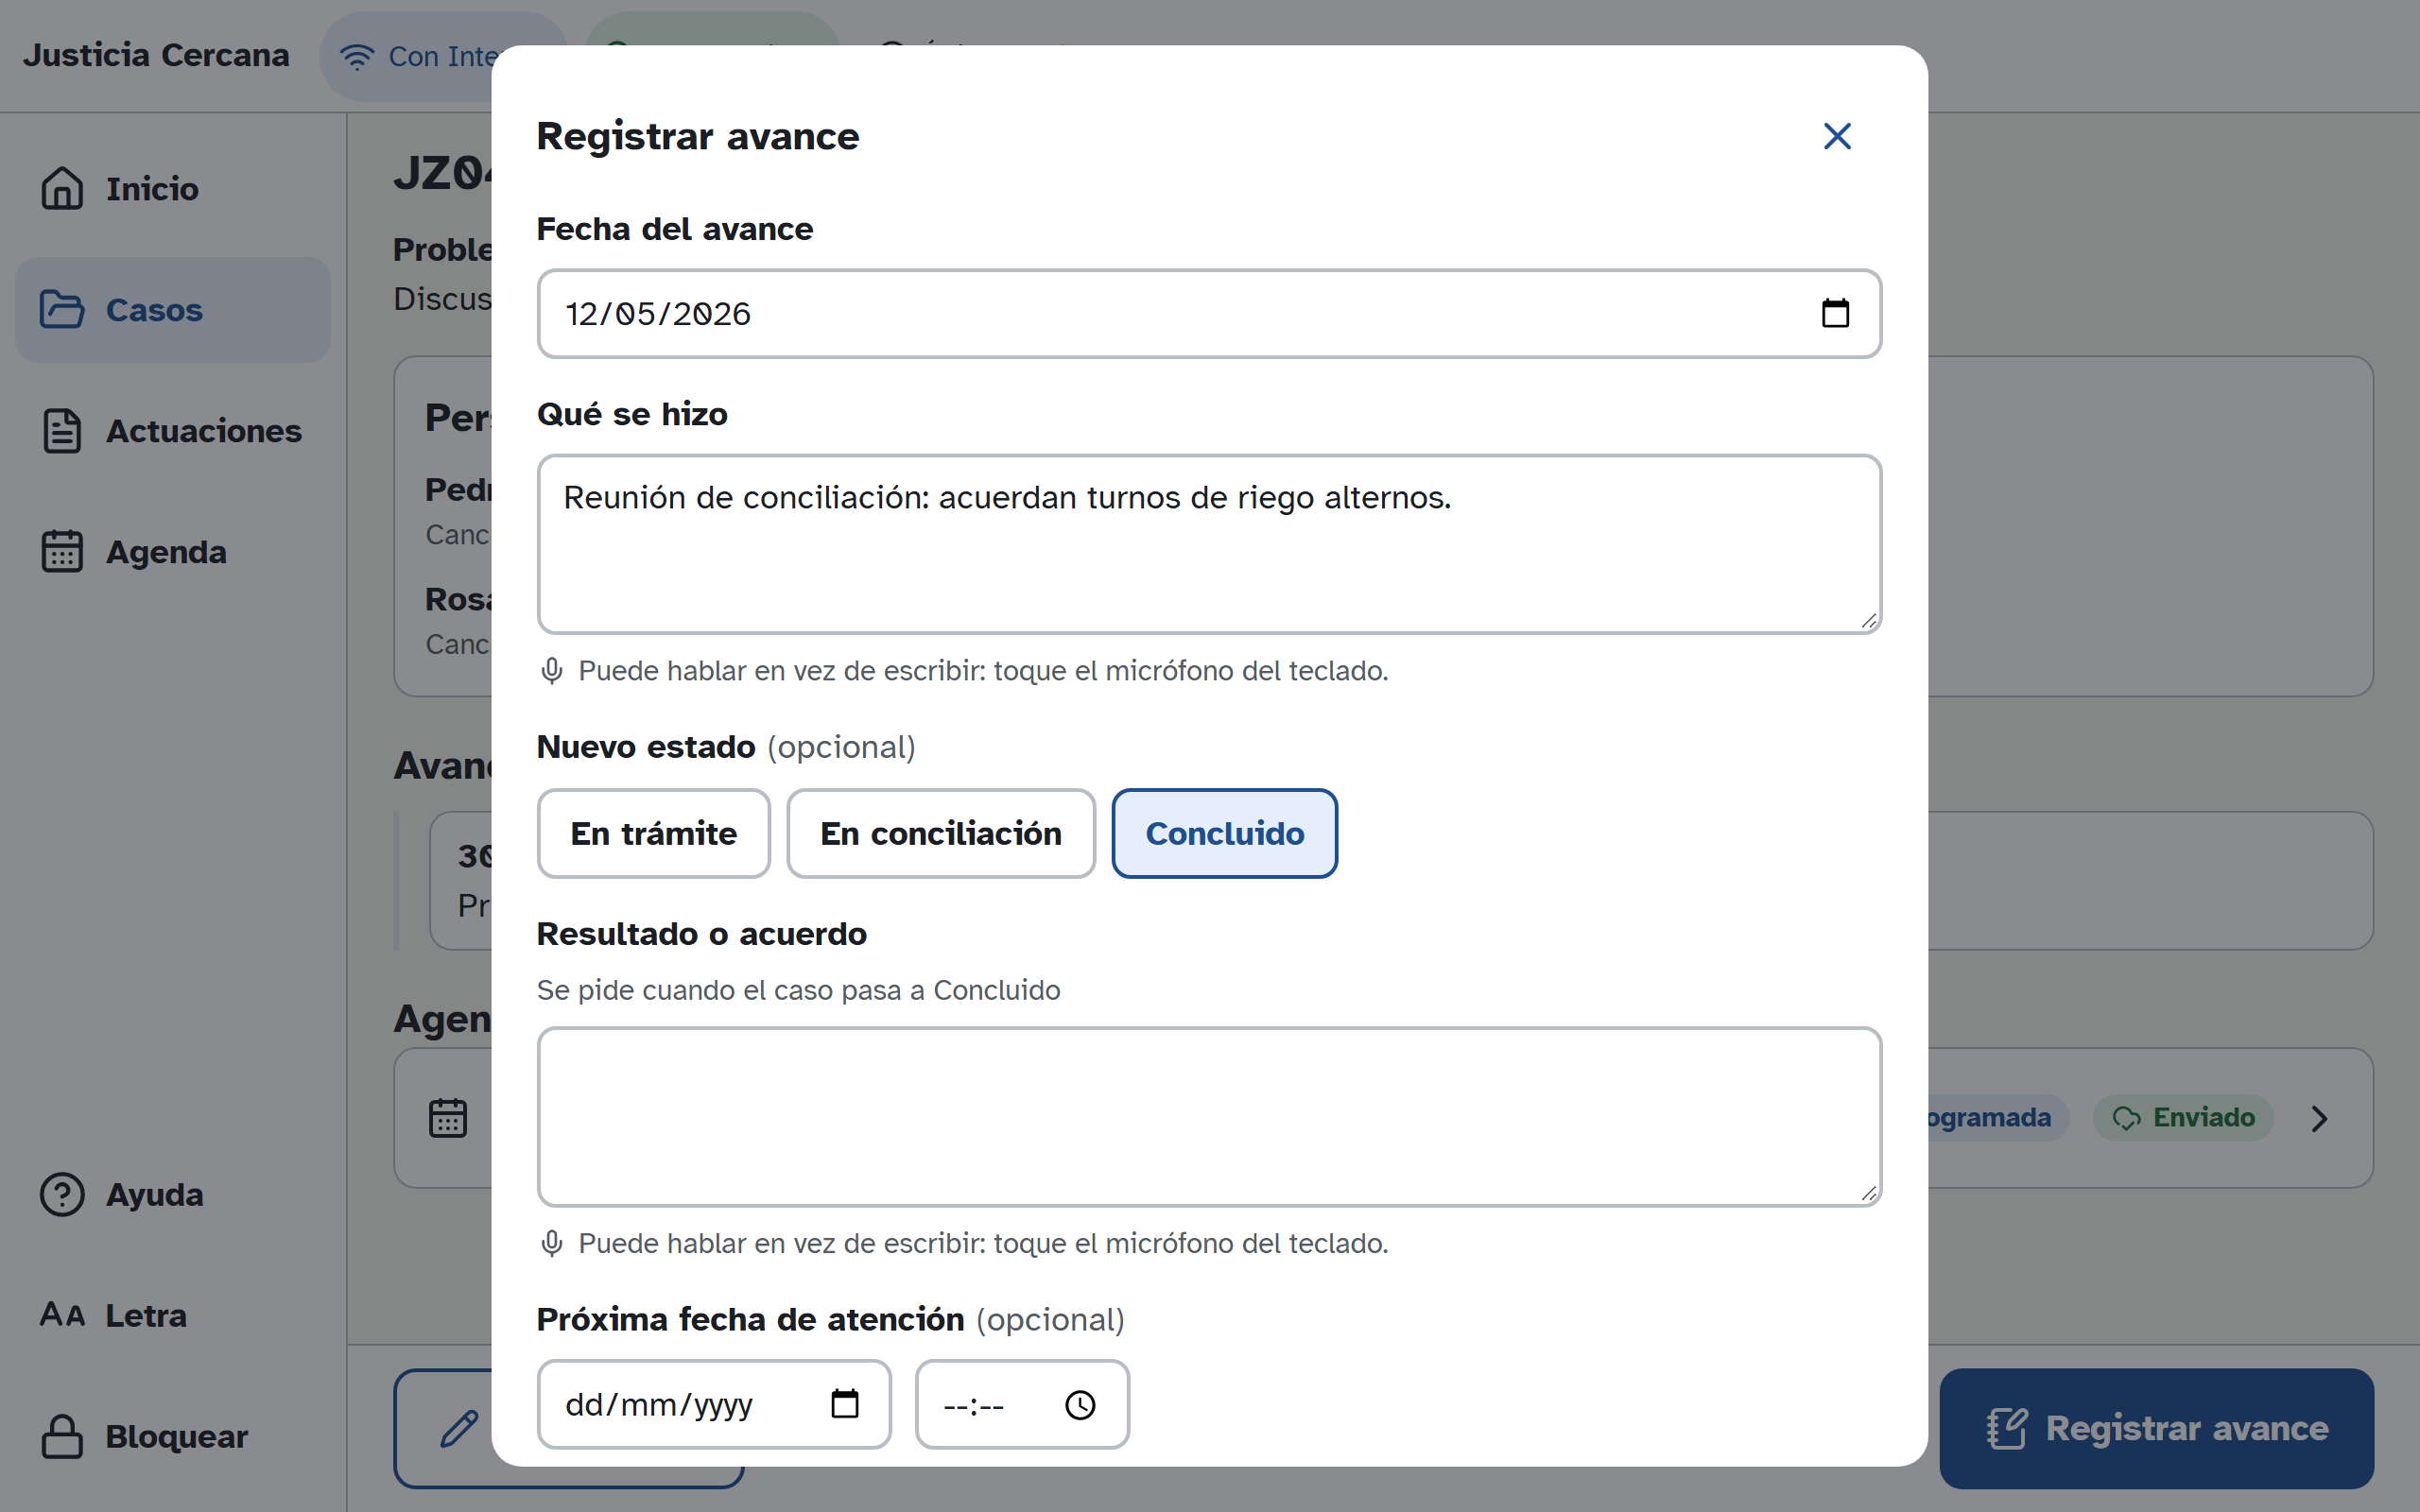
\includegraphics[width=\linewidth]{../../captures/FA-03a_registrar-avance.png}\\[-2pt]{\footnotesize\raggedright\textbf{P-04 · 3.} Ventana ``Registrar avance'' con condicional de acuerdo al pasar a Concluido \emph{(Cobertura y funcionamiento de los módulos)}\par}\end{minipage}\hfill
\begin{minipage}[t]{0.49\textwidth}\centering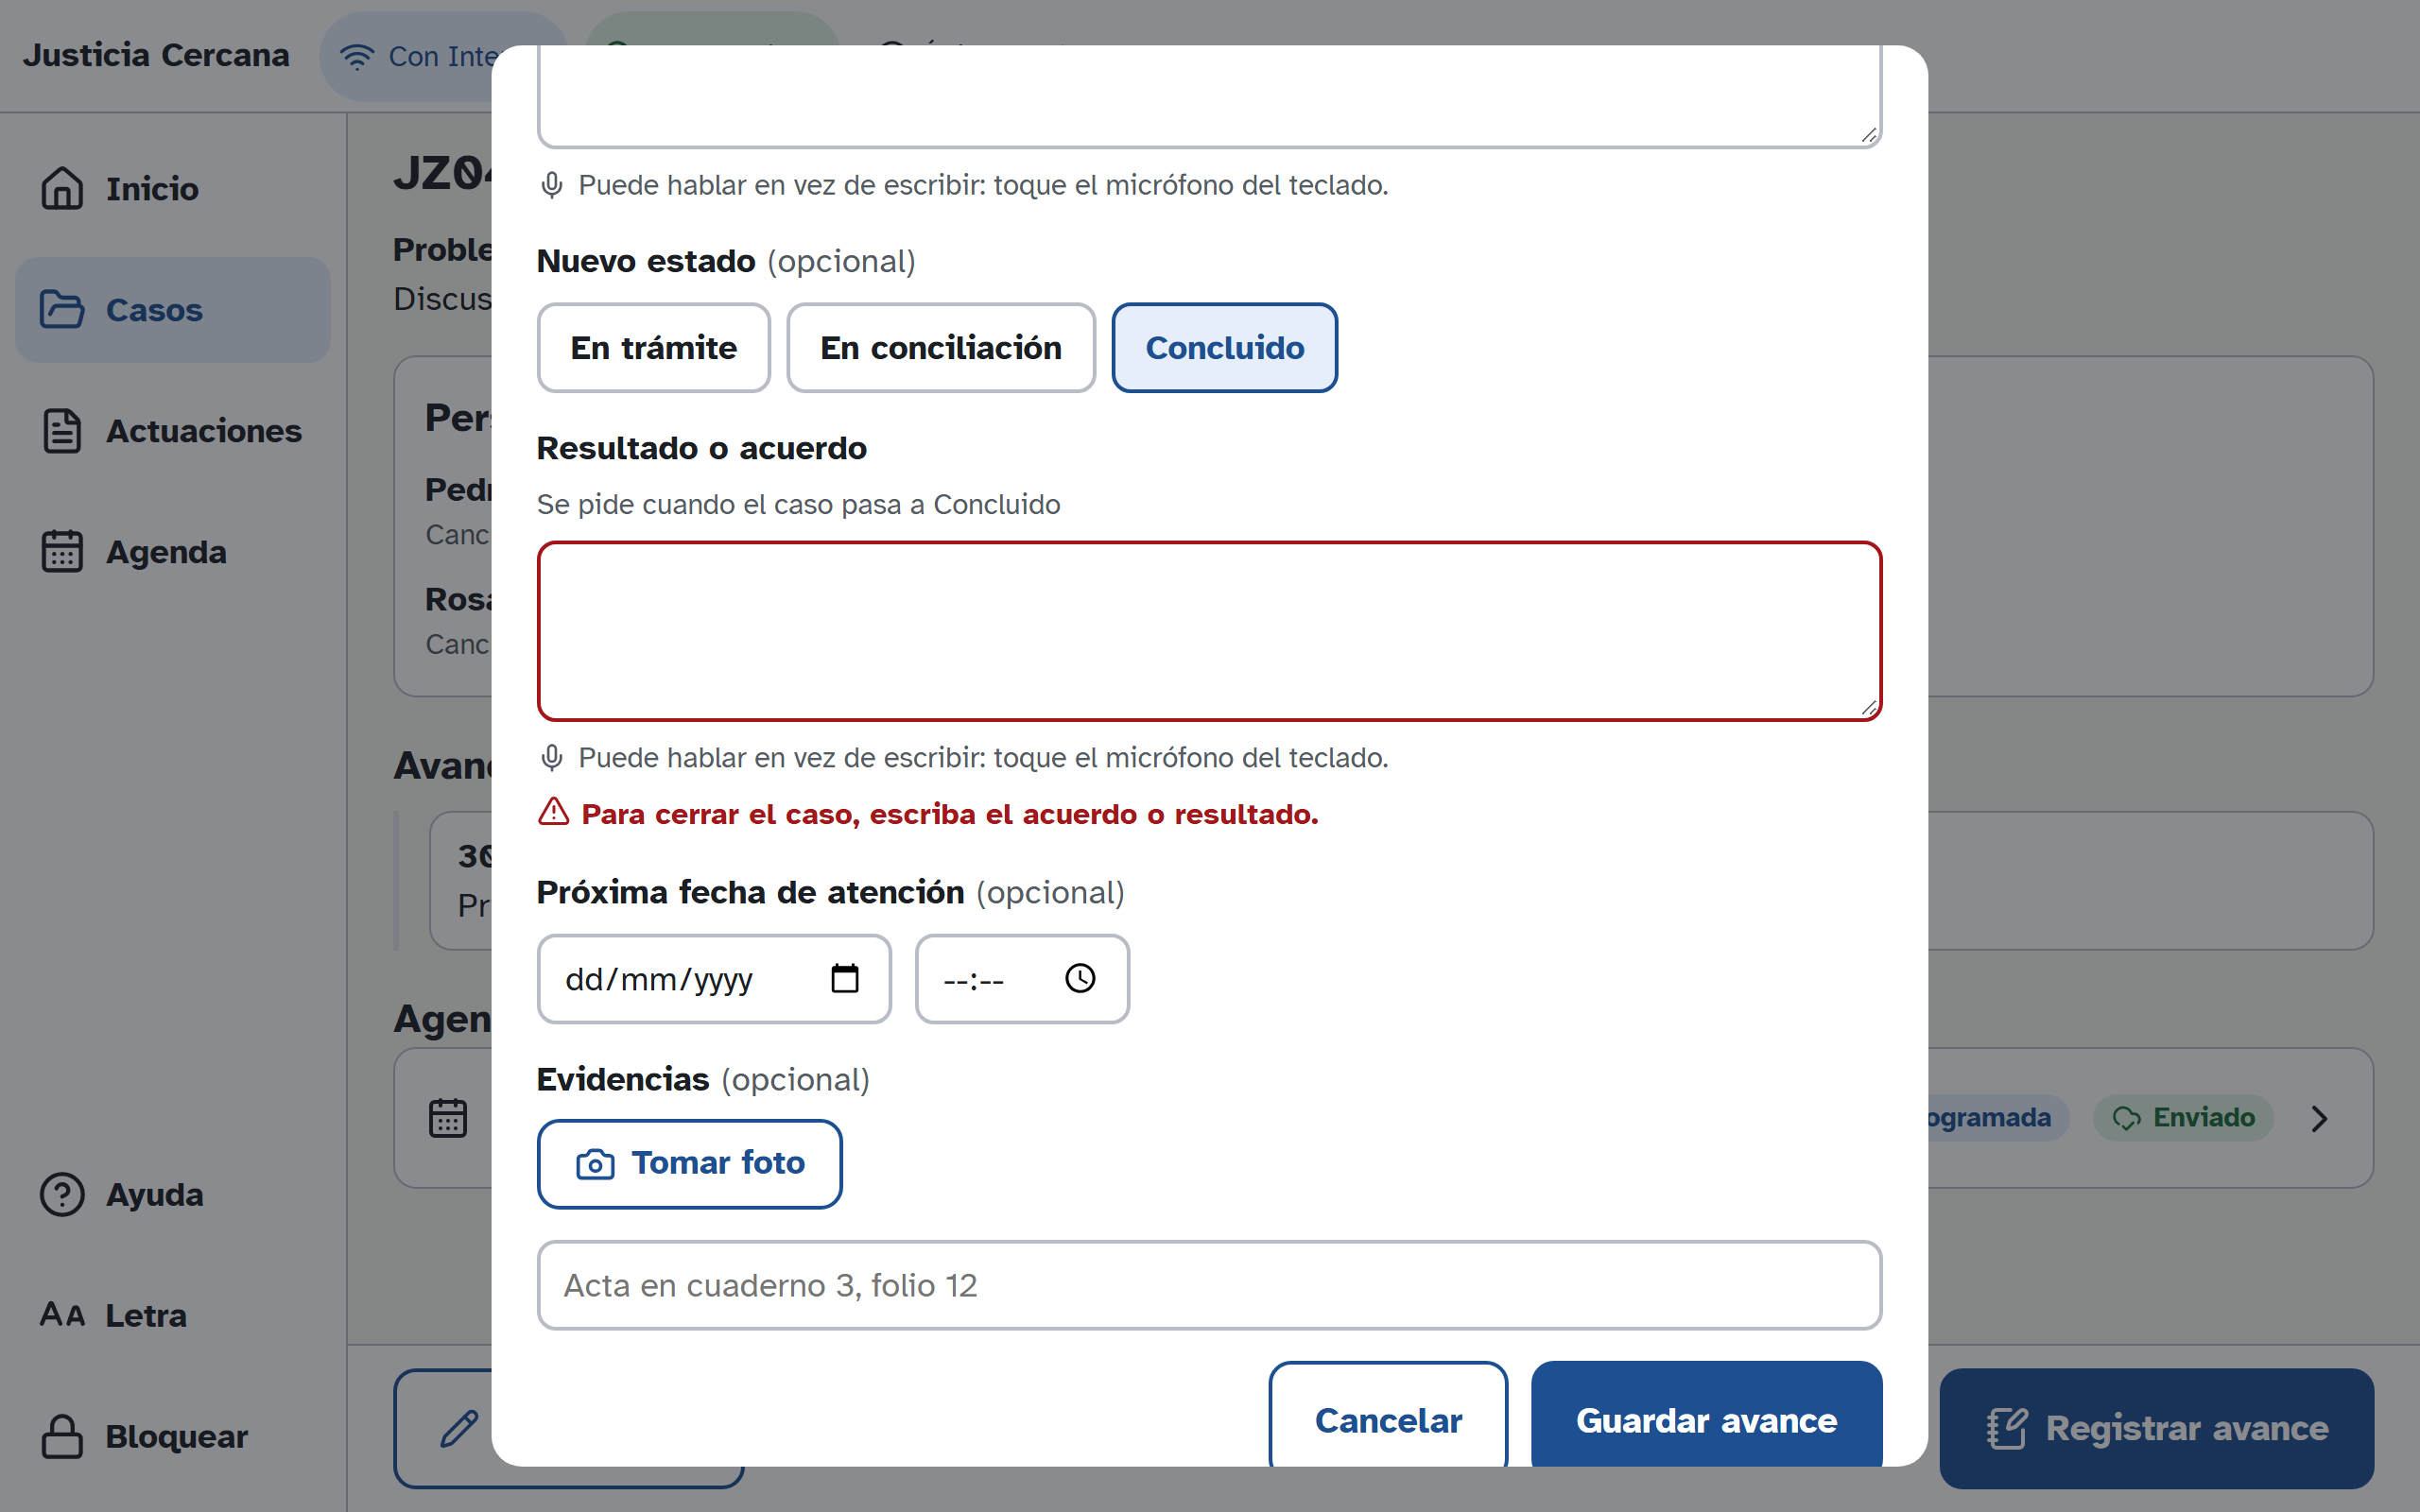
\includegraphics[width=\linewidth]{../../captures/FA-03b_exige-acuerdo.png}\\[-2pt]{\footnotesize\raggedright\textbf{P-04 · 3.} Concluido exige el acuerdo (mensaje en lenguaje simple) \emph{(Principios de diseño y heurísticas)}\par}\end{minipage}\par\vspace{8pt}\noindent
\begin{minipage}[t]{0.49\textwidth}\centering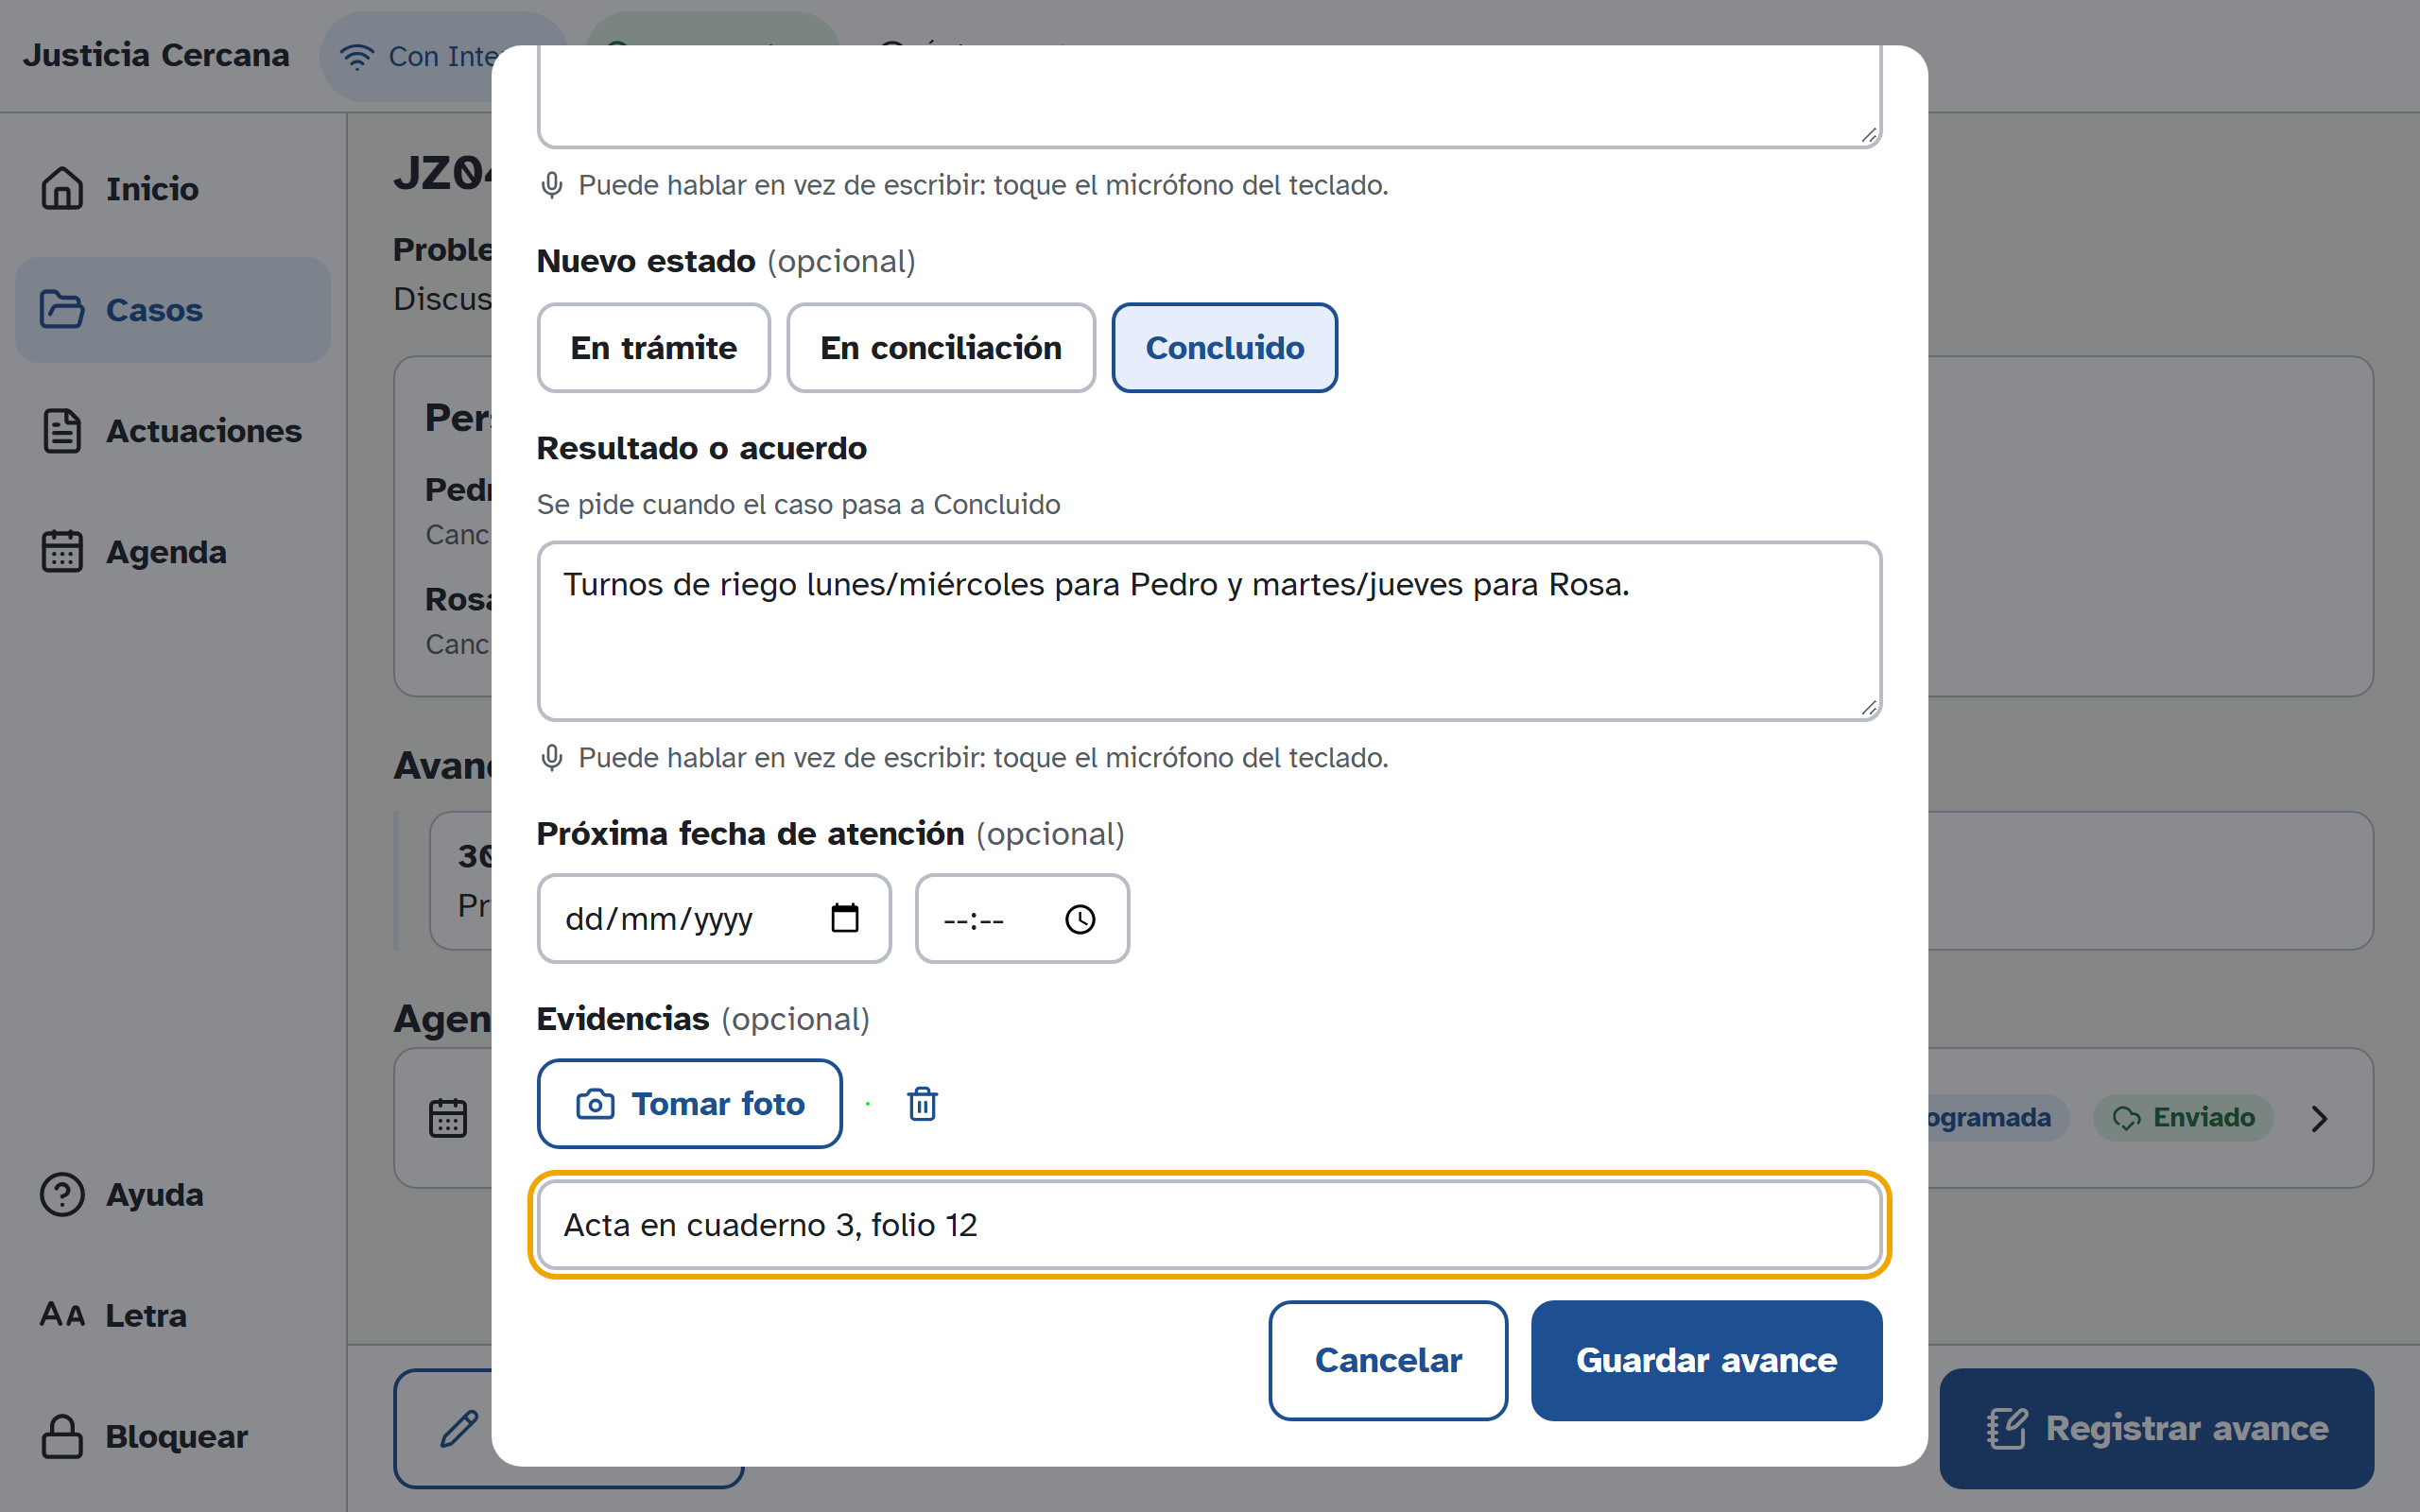
\includegraphics[width=\linewidth]{../../captures/FA-03c_foto-acta.png}\\[-2pt]{\footnotesize\raggedright\textbf{P-04 · 3.} Acuerdo escrito y foto del acta adjunta + referencia física \emph{(Cobertura y funcionamiento de los módulos)}\par}\end{minipage}\hfill
\begin{minipage}[t]{0.49\textwidth}\centering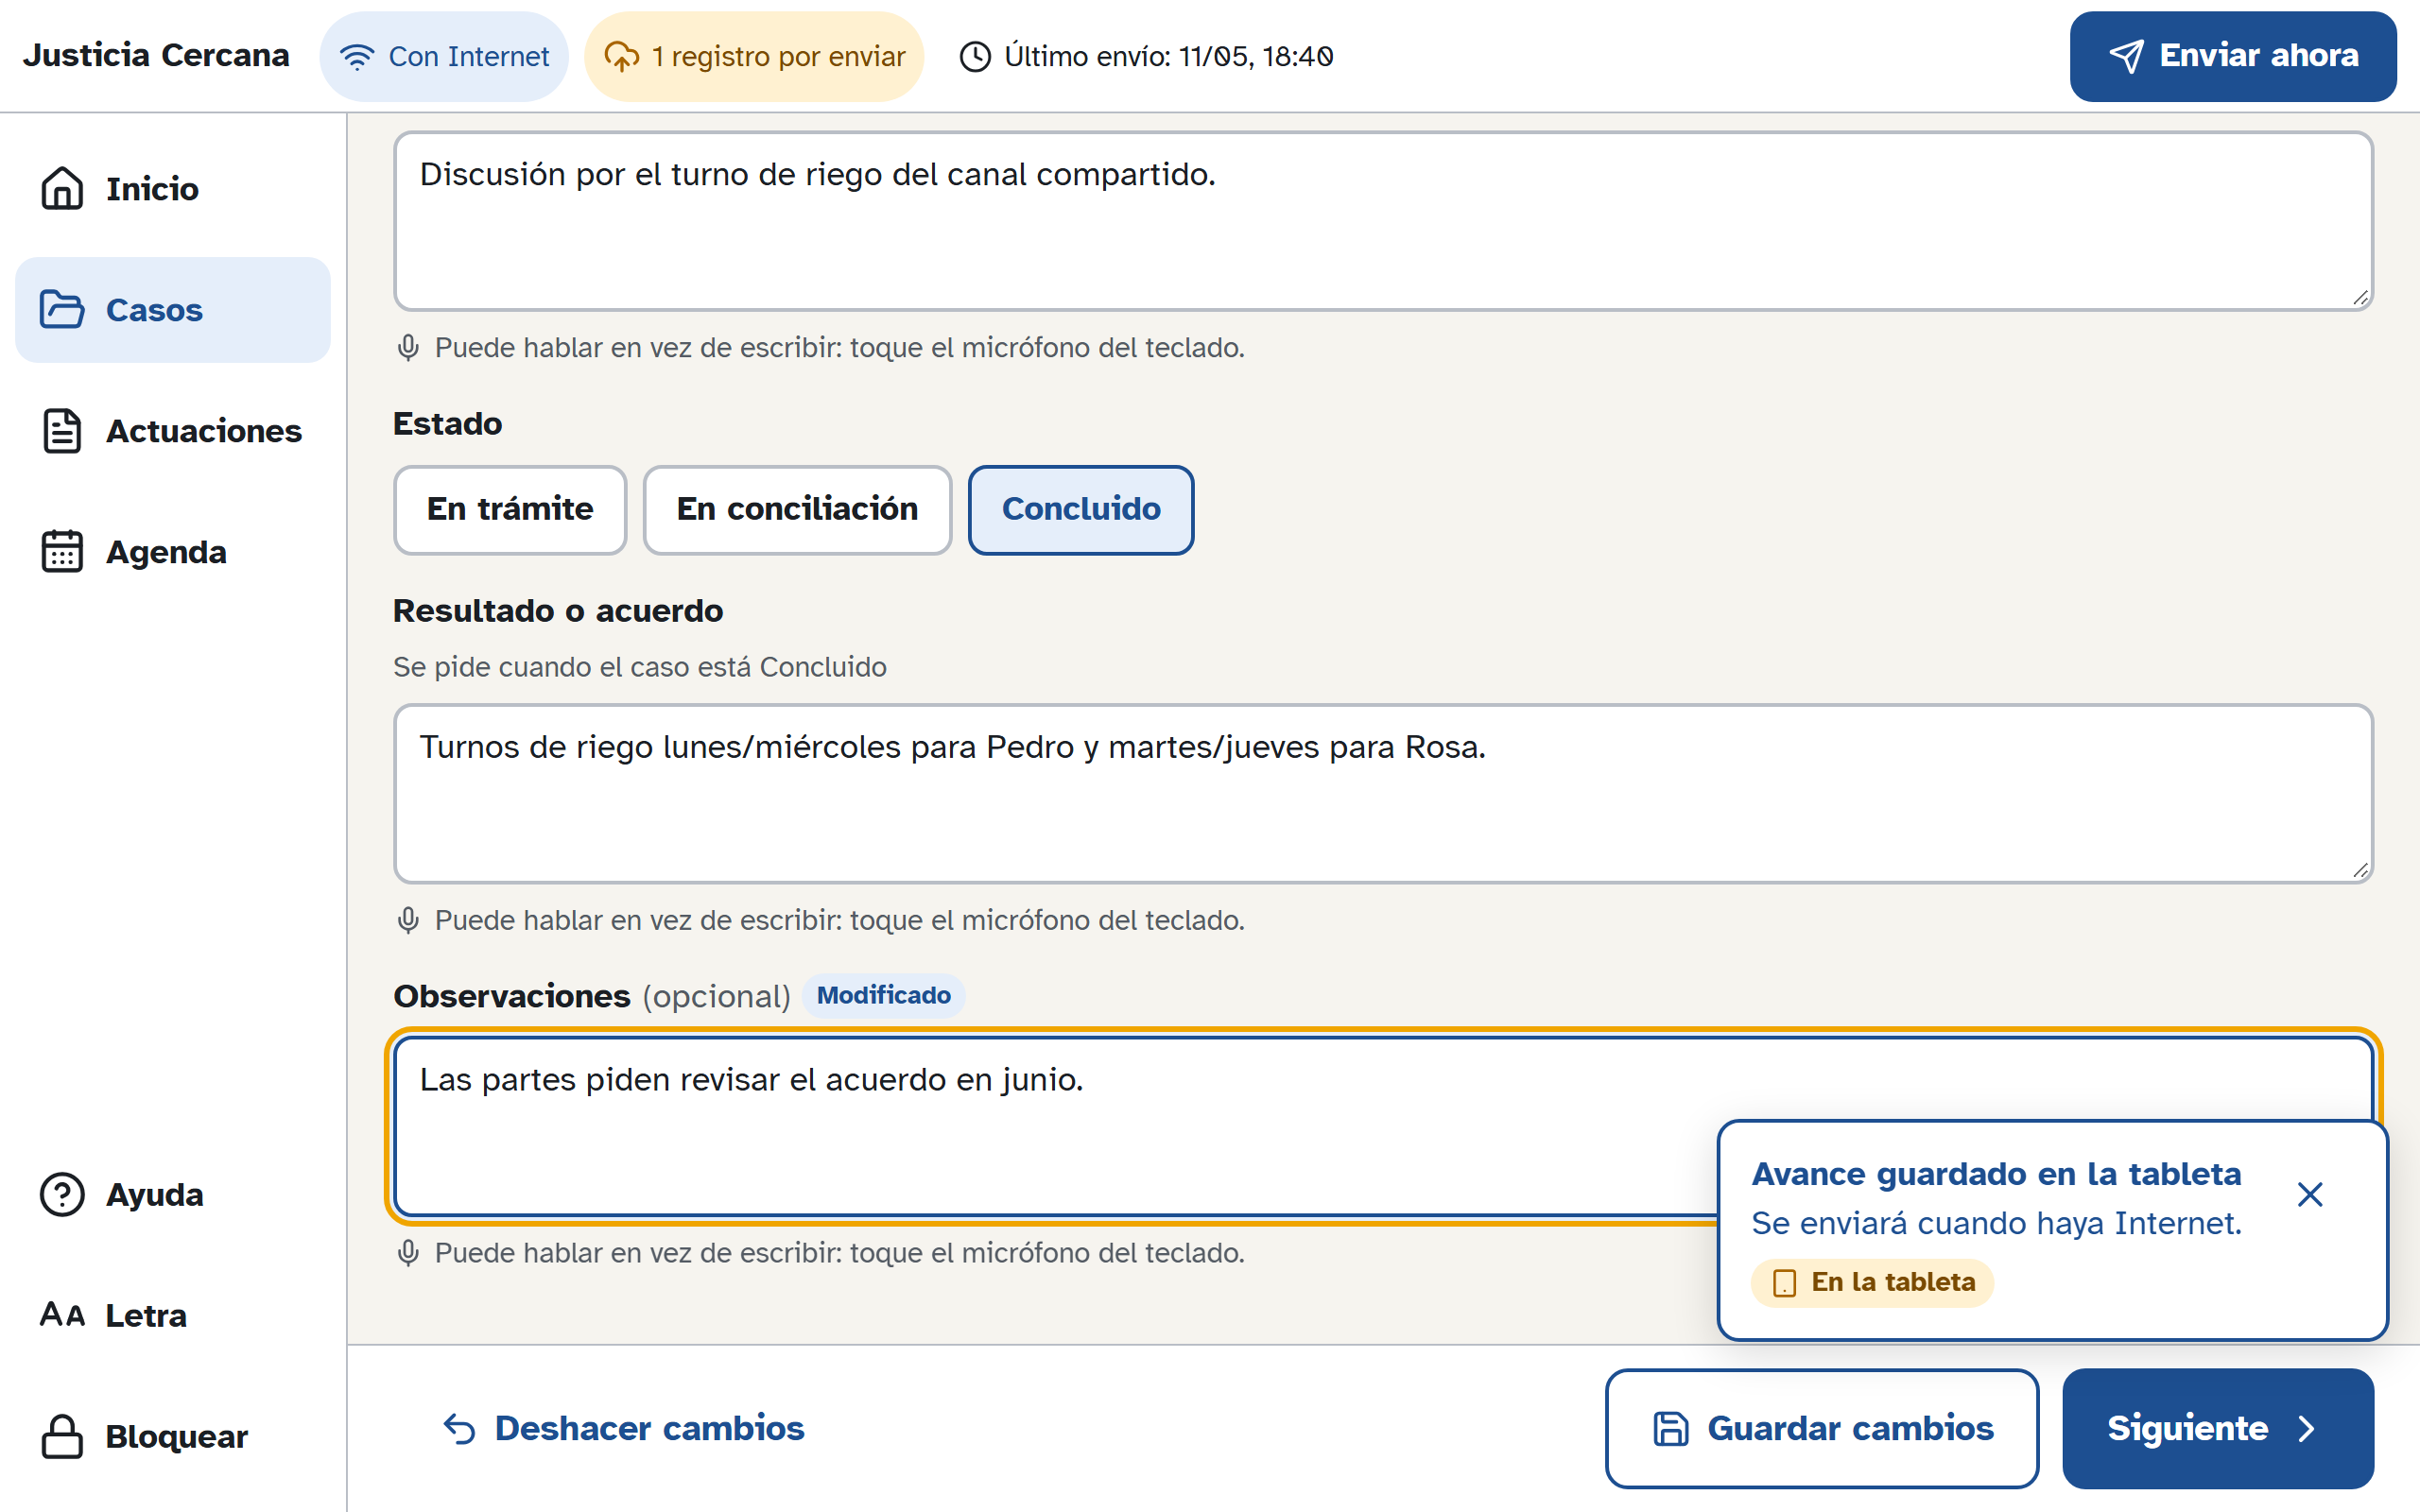
\includegraphics[width=\linewidth]{../../captures/FA-04a_modificado.png}\\[-2pt]{\footnotesize\raggedright\textbf{P-03 · 4.} Campo editado resaltado con ``Modificado'' y botón [Deshacer cambios] \emph{(Principios de diseño y heurísticas)}\par}\end{minipage}\par\vspace{8pt}\noindent
\begin{minipage}[t]{0.49\textwidth}\centering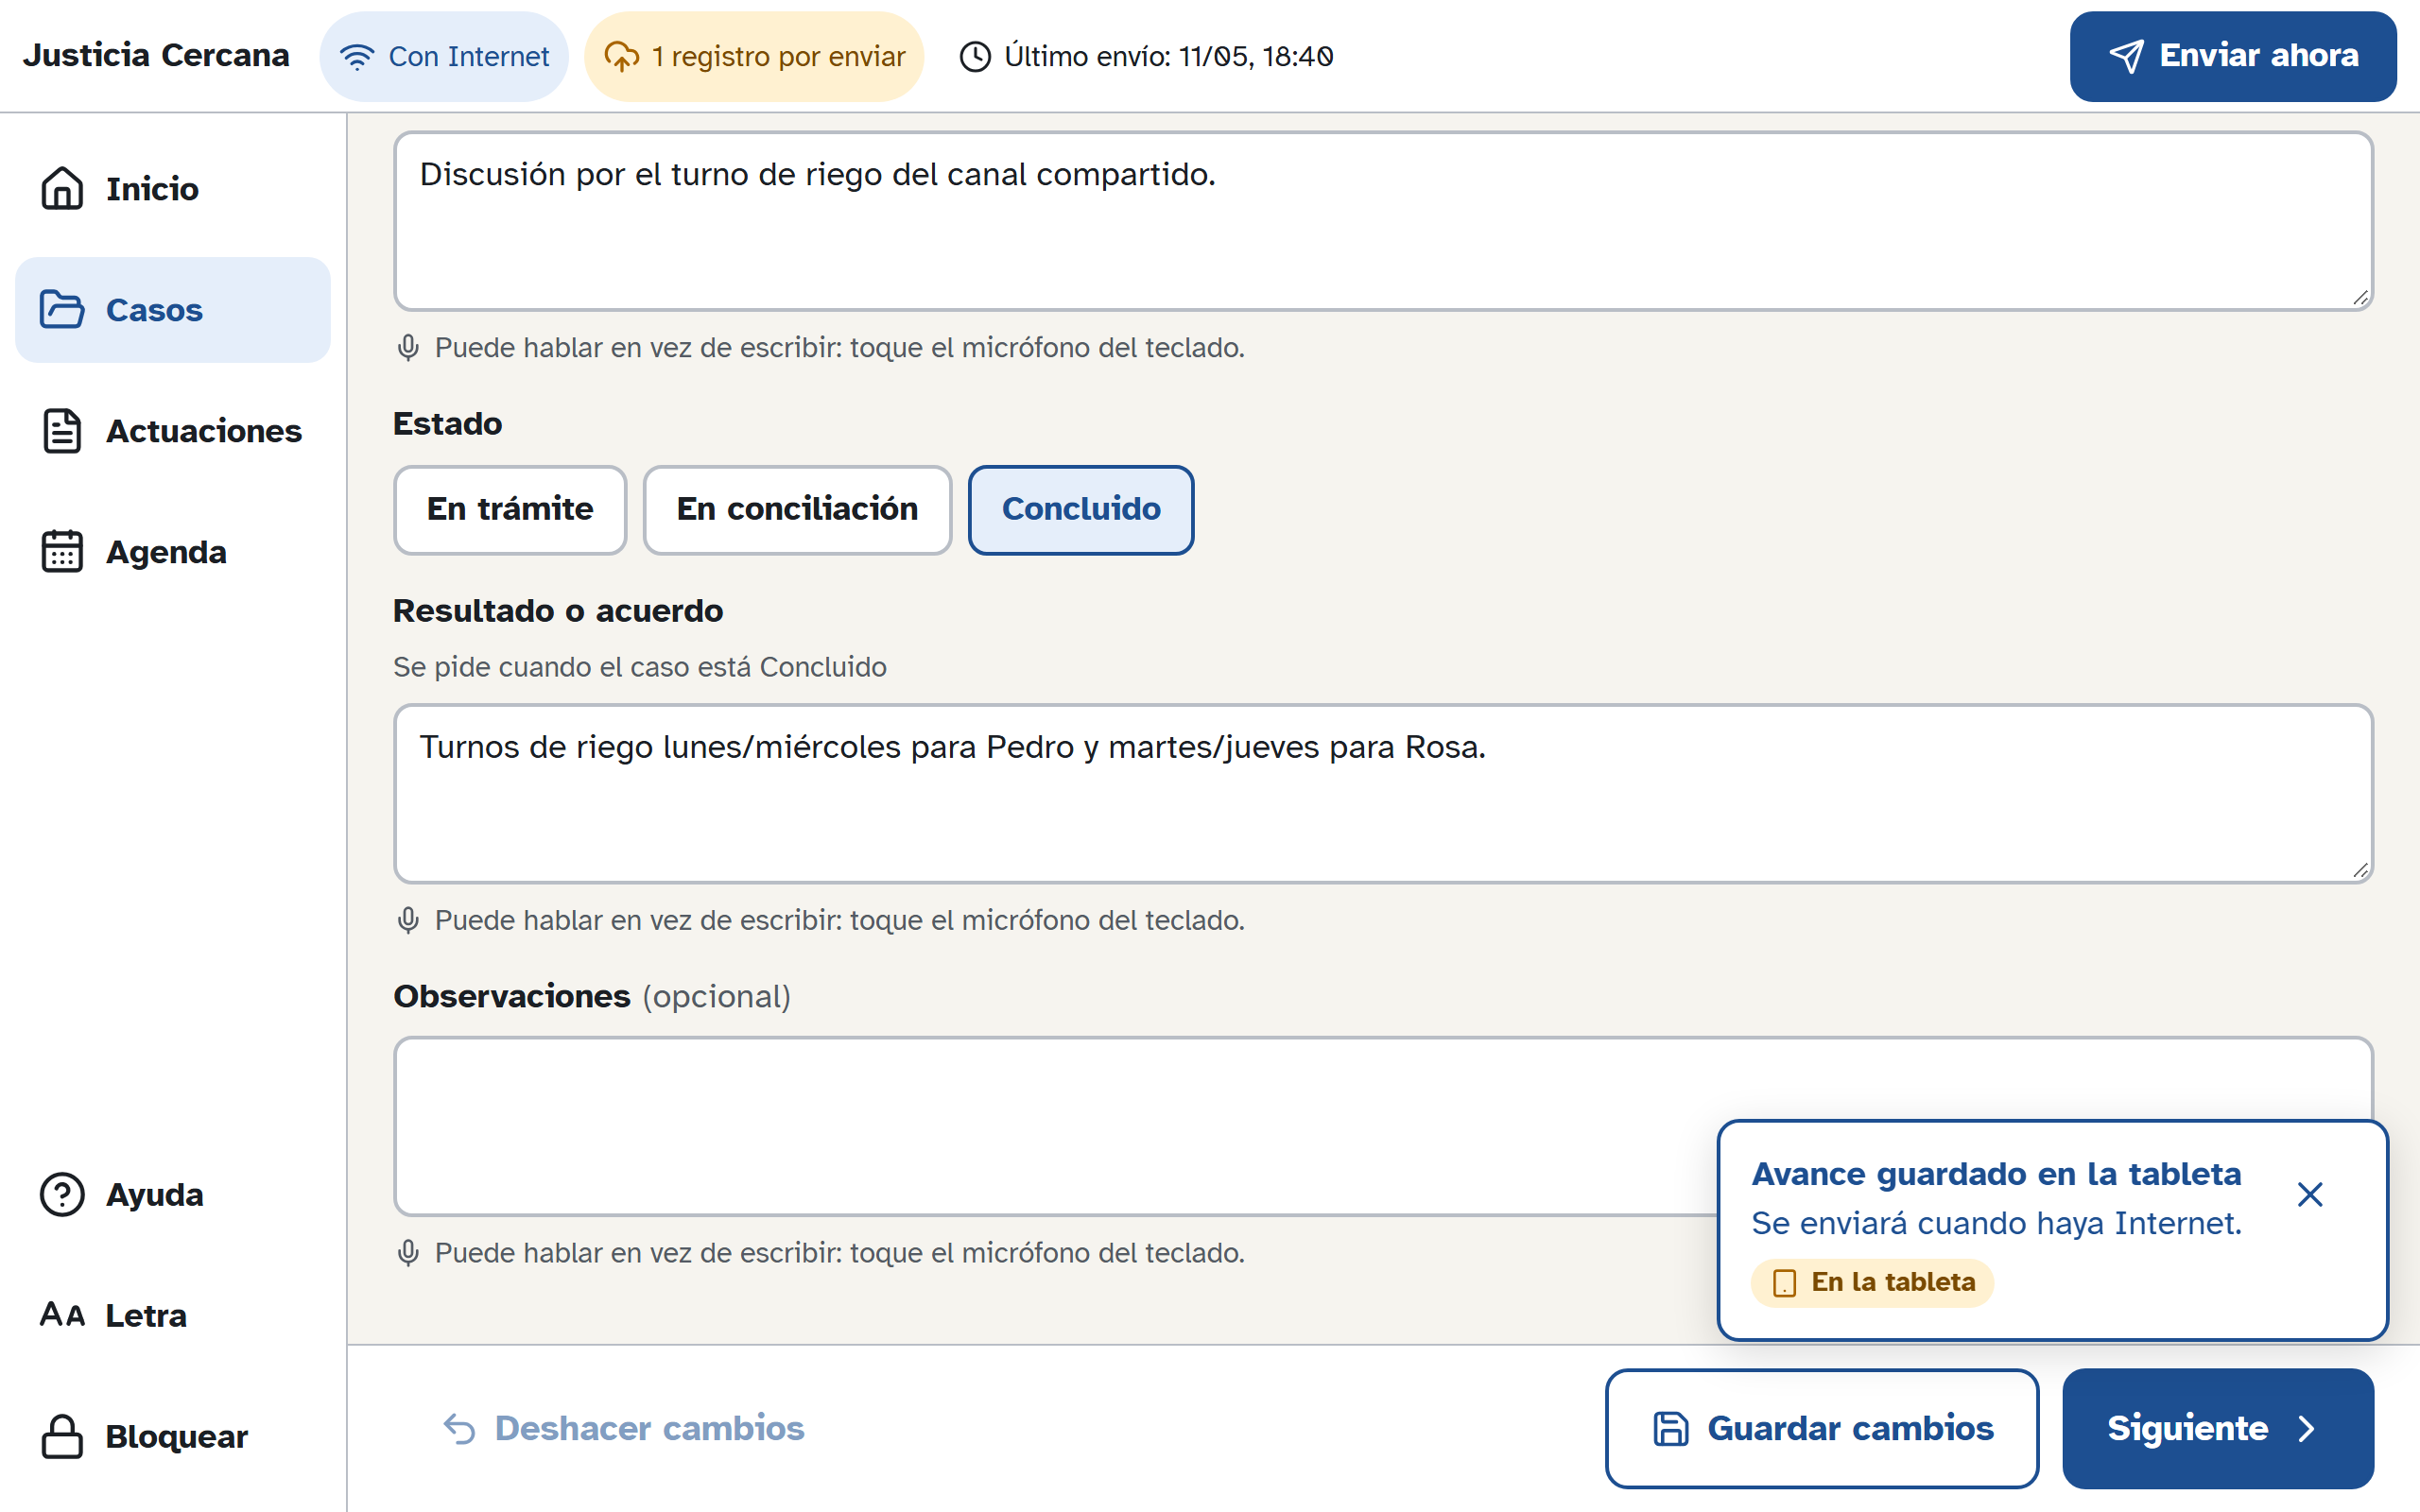
\includegraphics[width=\linewidth]{../../captures/FA-04b_deshacer.png}\\[-2pt]{\footnotesize\raggedright\textbf{P-03 · 4.} [Deshacer cambios] devuelve el valor original \emph{(Principios de diseño y heurísticas)}\par}\end{minipage}\hfill
\begin{minipage}[t]{0.49\textwidth}\centering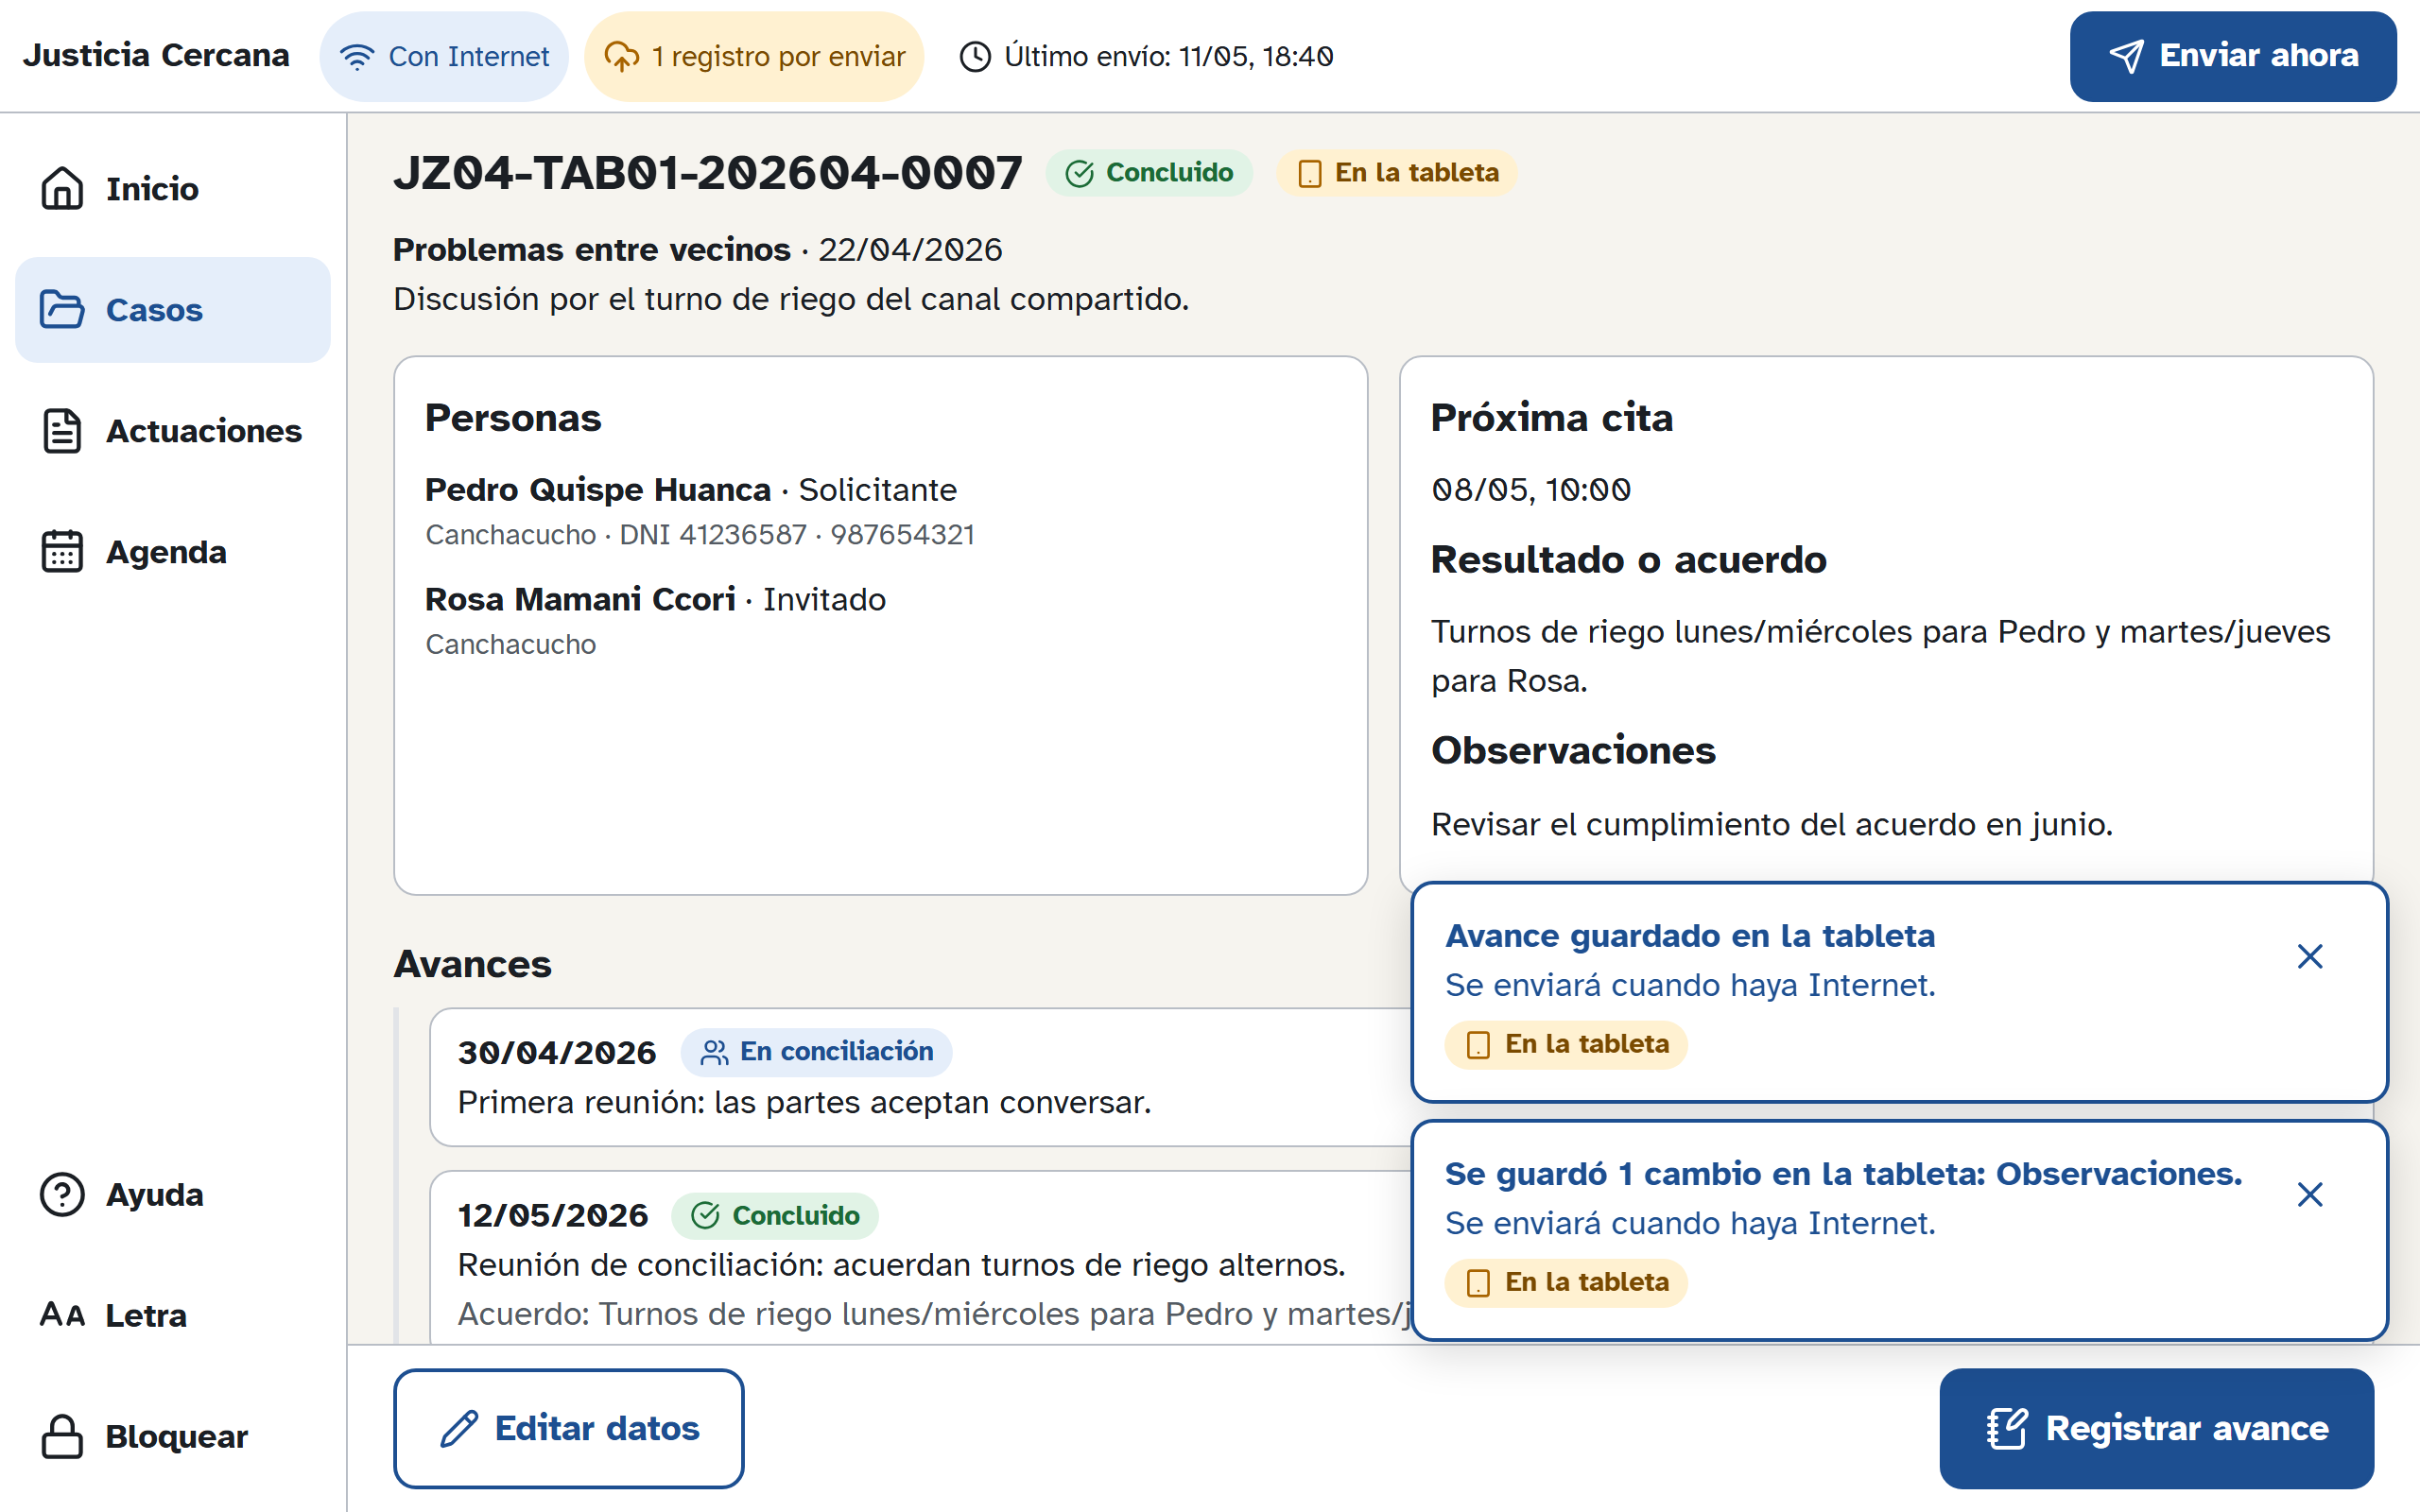
\includegraphics[width=\linewidth]{../../captures/FA-04c_confirmacion-cambios.png}\\[-2pt]{\footnotesize\raggedright\textbf{P-04 · 4.} ``Se guardó 1 cambio en la tableta: Observaciones.'' \emph{(Funcionamiento sin conexión)}\par}\end{minipage}\par\vspace{8pt}\noindent
\par\vspace{4pt}
\subsection*{Flujo B}
\noindent
\begin{minipage}[t]{0.49\textwidth}\centering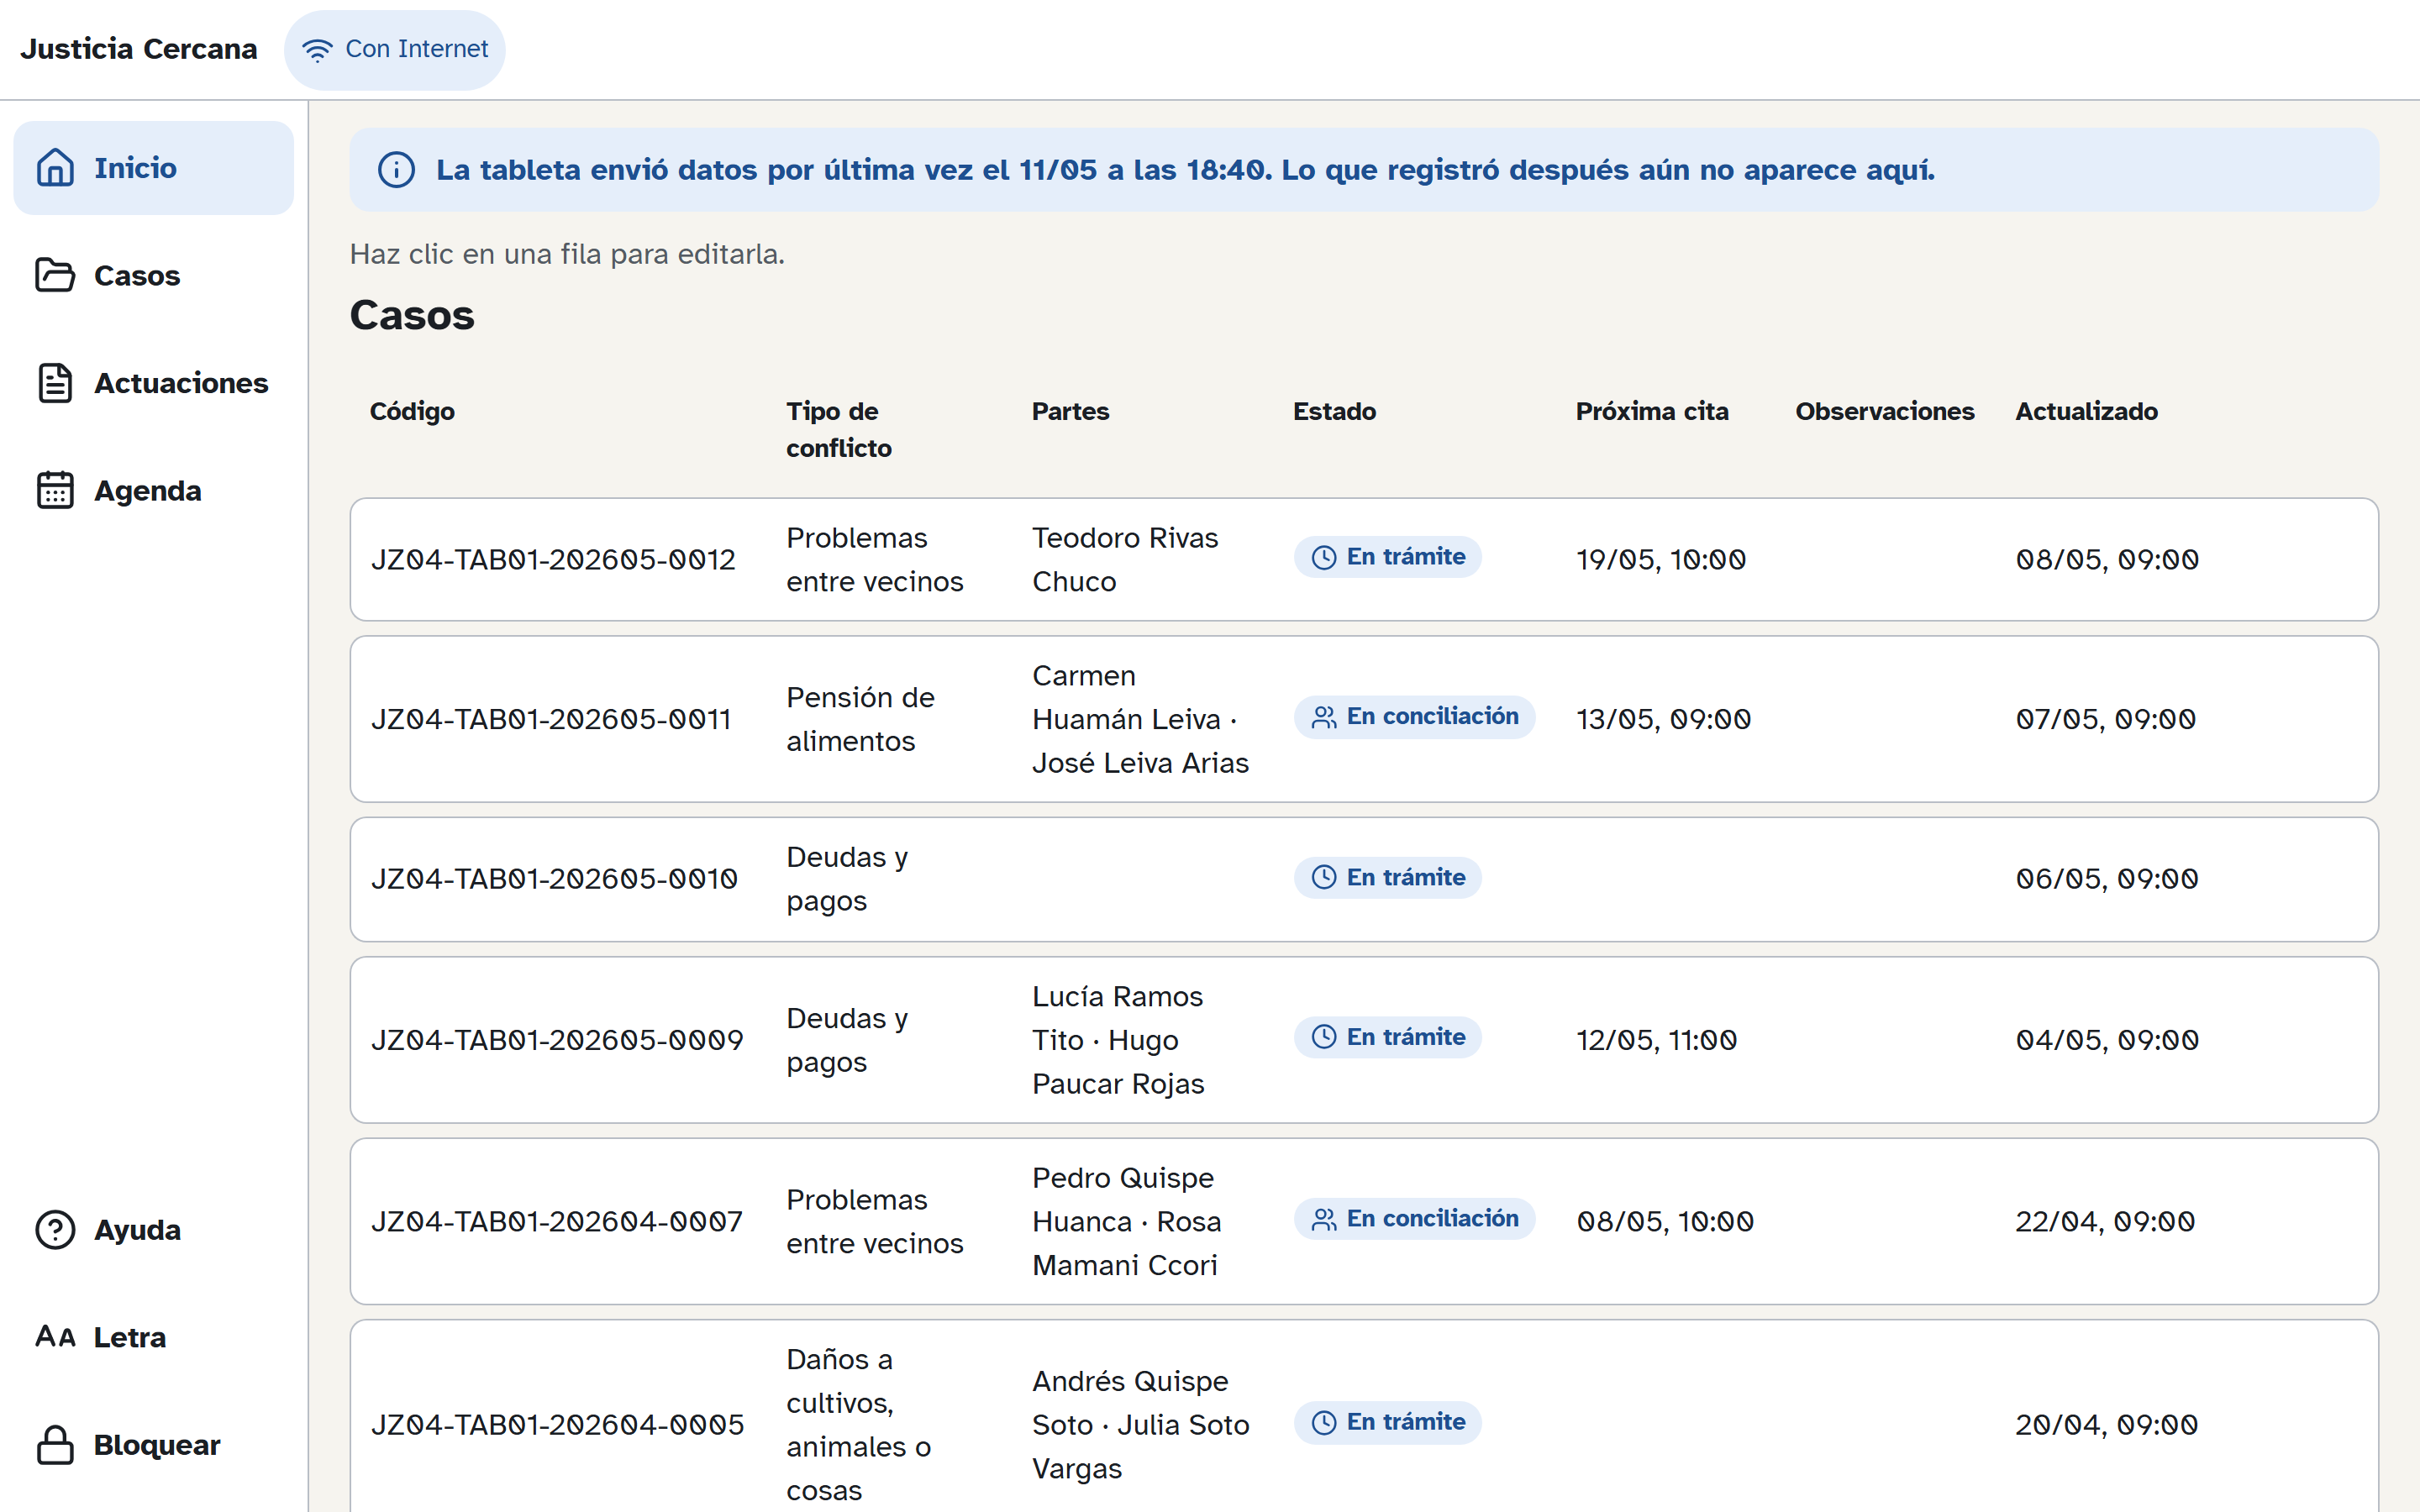
\includegraphics[width=\linewidth]{../../captures/FB-01_computadora-aviso.png}\\[-2pt]{\footnotesize\raggedright\textbf{P-10 · 1.} Vista en computadora 1440×900 con aviso del último envío; no afirma pendientes de la tableta \emph{(Funcionamiento sin conexión)}\par}\end{minipage}\hfill
\begin{minipage}[t]{0.49\textwidth}\centering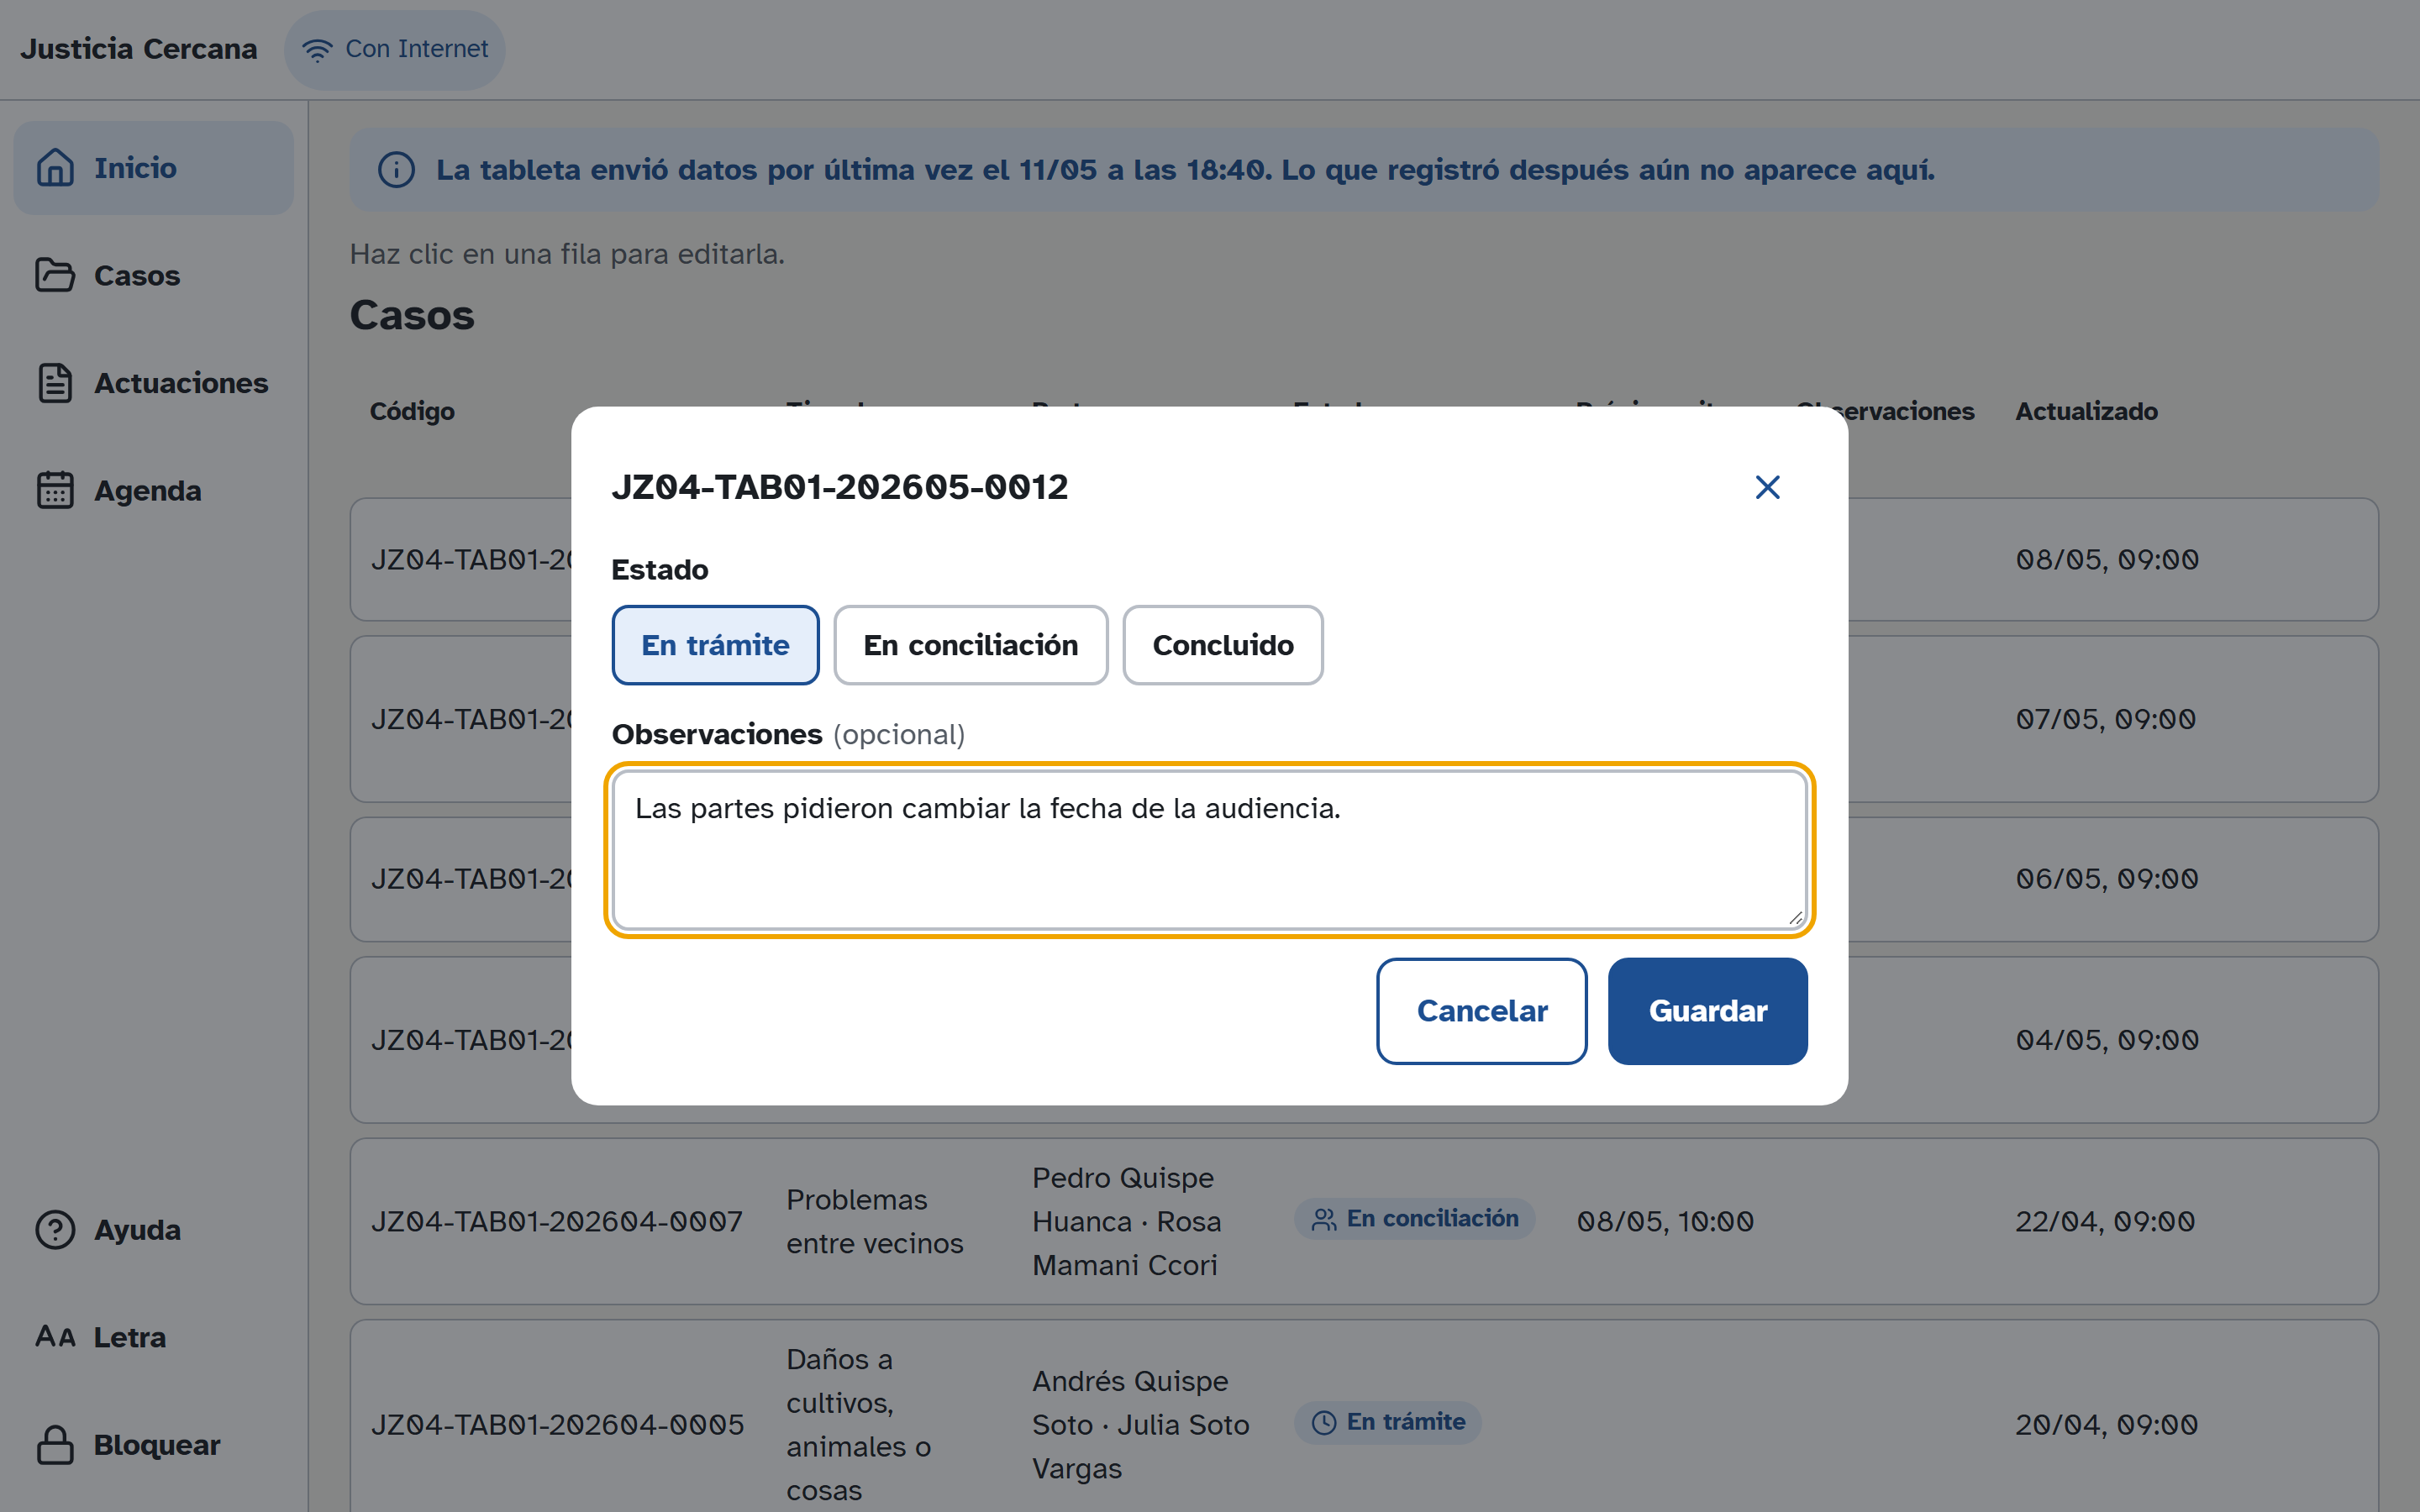
\includegraphics[width=\linewidth]{../../captures/FB-02_editar-caso.png}\\[-2pt]{\footnotesize\raggedright\textbf{P-10 · 2.} Edición de un caso desde la computadora (origen de conflicto) \emph{(Cobertura y funcionamiento de los módulos)}\par}\end{minipage}\par\vspace{8pt}\noindent
\begin{minipage}[t]{0.49\textwidth}\centering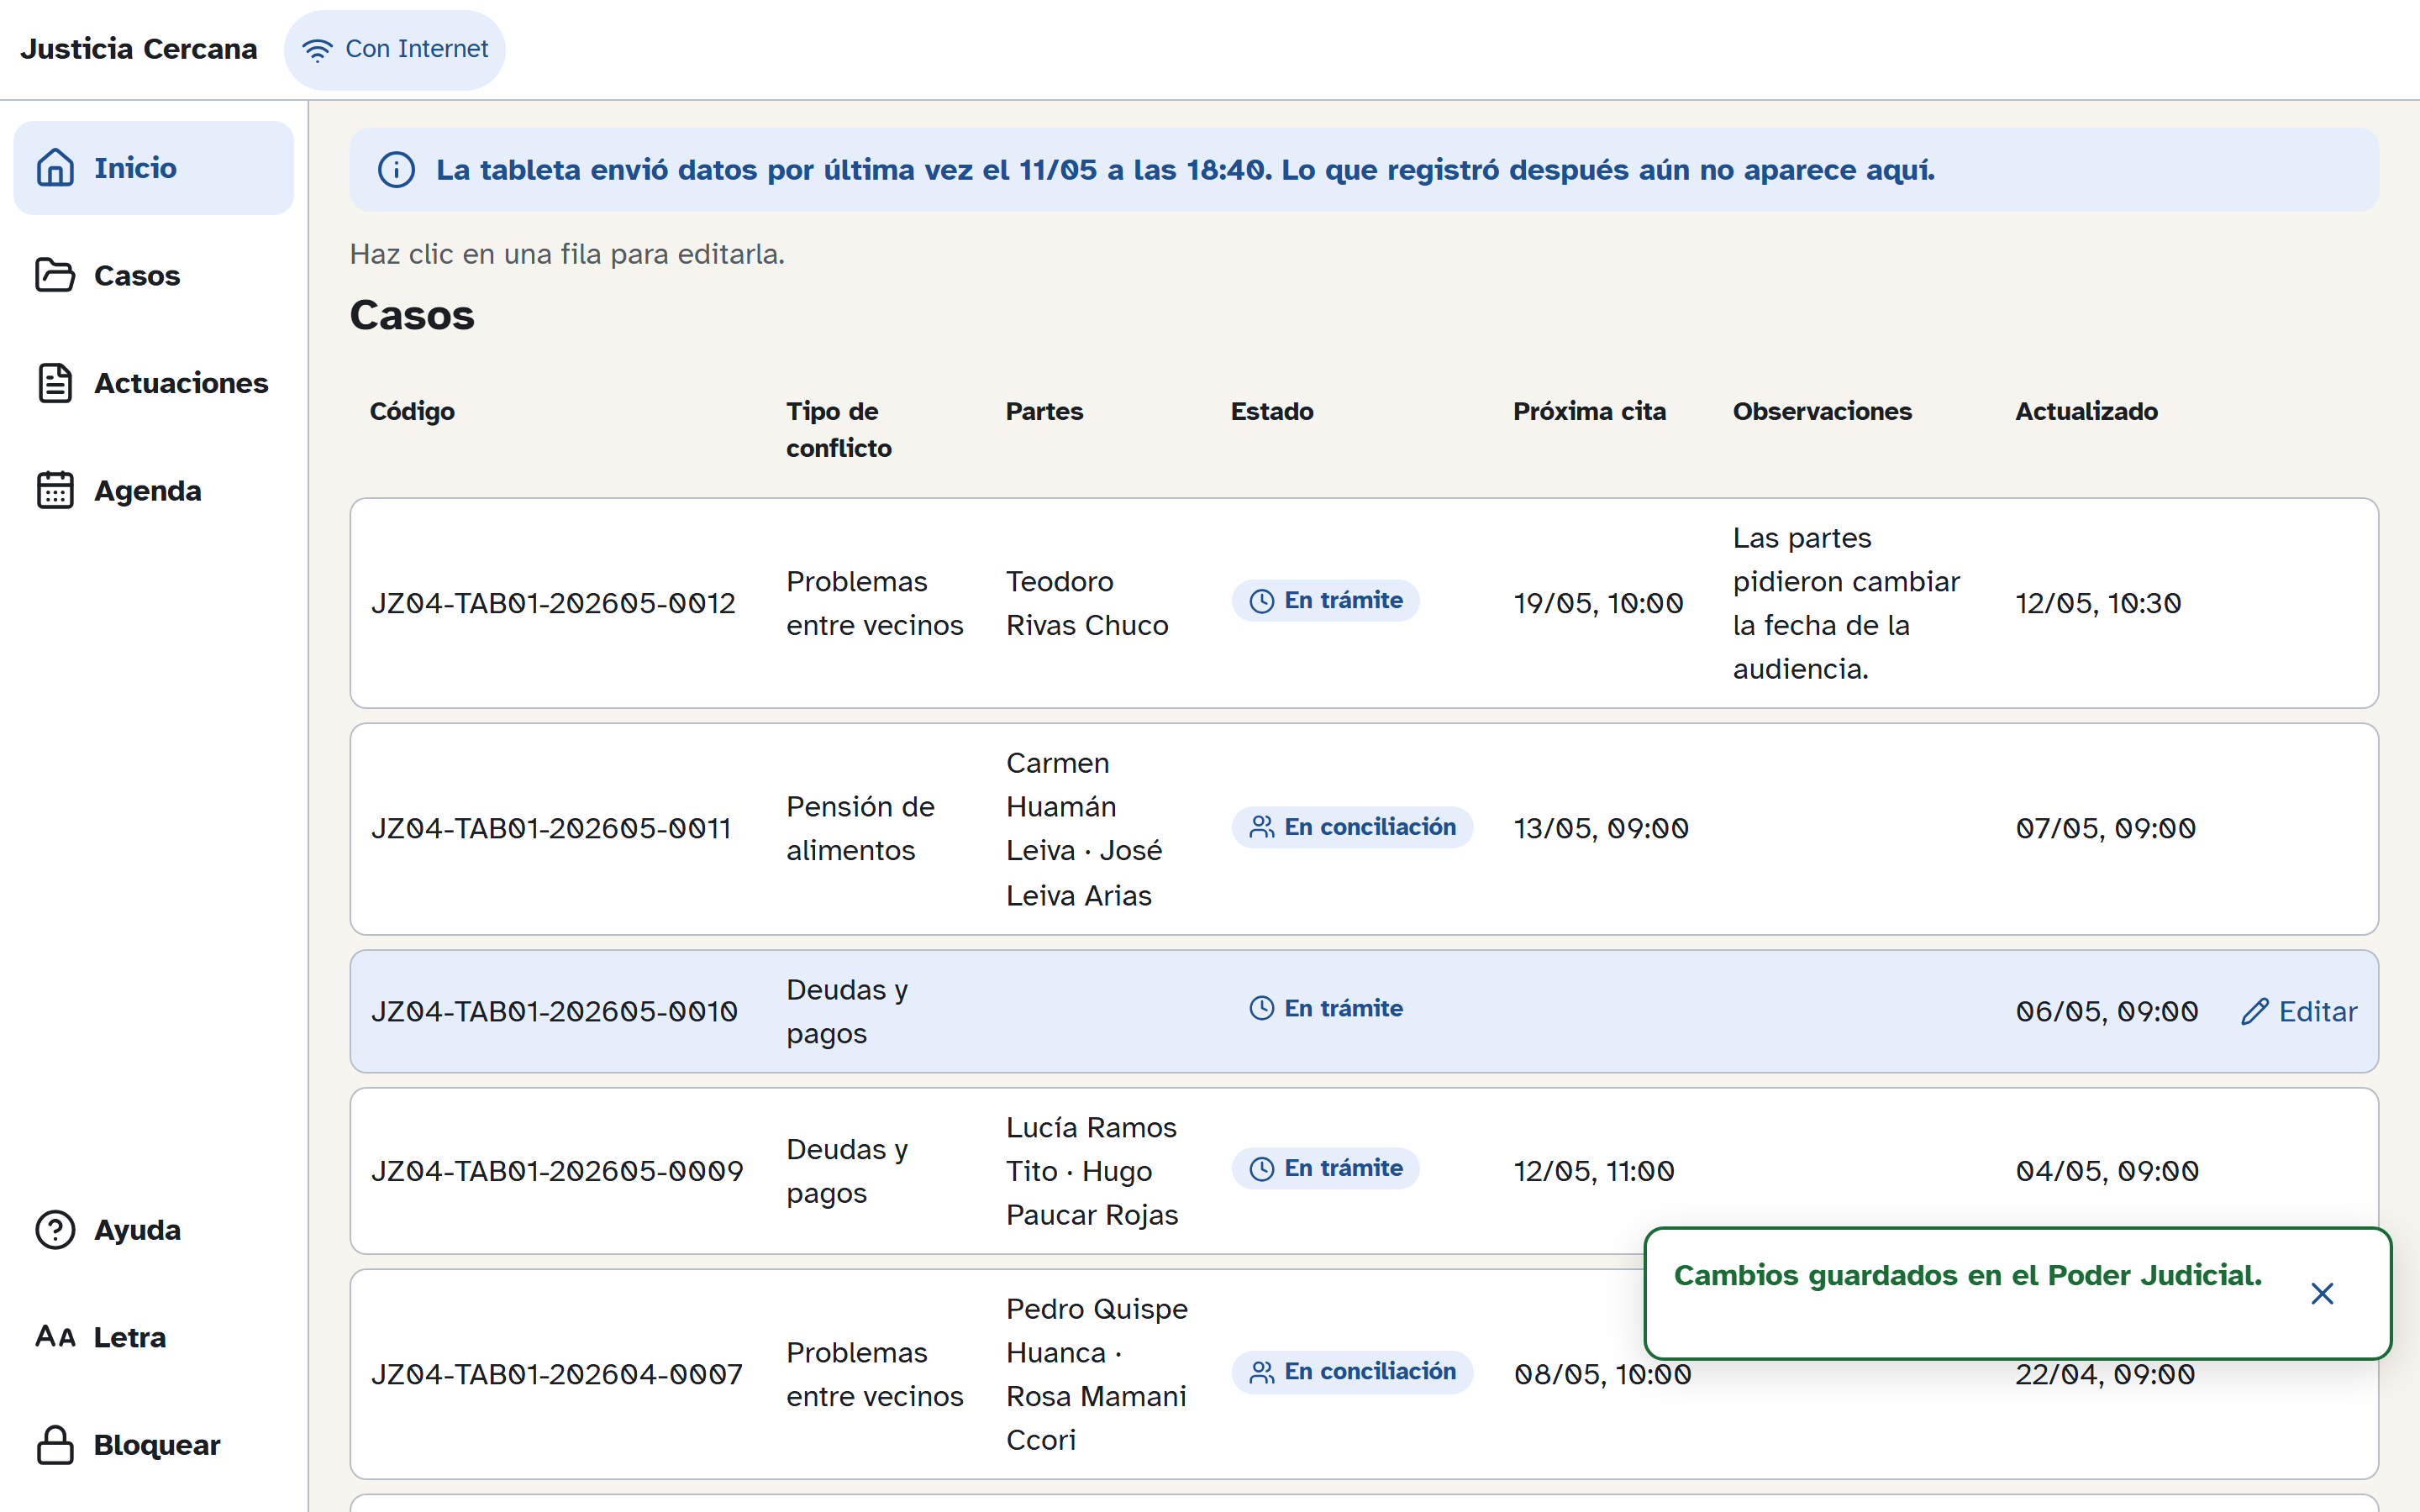
\includegraphics[width=\linewidth]{../../captures/FB-03_guardado-computadora.png}\\[-2pt]{\footnotesize\raggedright\textbf{P-10 · 2.} Cambio guardado en el Poder Judicial \emph{(Cobertura y funcionamiento de los módulos)}\par}\end{minipage}\hfill
\par\vspace{4pt}


% ---------------------------------------------------------------- 9
\section{Matriz de justificación}
Una fila por elemento; el ID coincide con el marcador del modo anotado (\texttt{?annotate=1}).
\begin{scriptsize}
\begin{longtable}{|L{0.4cm}|L{1.3cm}|L{2.6cm}|L{2.3cm}|L{2.3cm}|L{1.9cm}|L{2.9cm}|}
\hline
\textbf{ID} & \textbf{Pantalla} & \textbf{Elemento} & \textbf{Necesidad} & \textbf{Norman / Nielsen} & \textbf{Factor humano} & \textbf{Cómo facilita o previene errores} \\ \hline
\endhead
1 & Global (barra de estado) & Indicador de conexión: ``Con Internet'' (azul, wifi) / ``Sin Internet · puede seguir trabajando'' (gris, wifi-off) & Saber en todo momento si hay Internet sin que la falta de señal, que es lo normal en campo, la alarme & Feedback / H1 Visibilidad del estado del sistema & Poca experiencia digital; trabajo en zonas sin cobertura & Sigue registrando sin detenerse ni pensar que algo falló, porque el gris y el texto ``puede seguir trabajando'' le dicen que sin Internet no se pierde nada \\ \hline
2 & Global (barra de estado) & Indicador de datos: ``3 registros por enviar'' (ámbar, cloud-upload) / ``Todo enviado'' (verde, cloud-check) & Saber si lo registrado ya llegó al Poder Judicial o sigue solo en la tableta & Feedback / H1 Visibilidad del estado; H4 Consistencia (ámbar = falta enviar en toda la app) & Carga de memoria de trabajo & No tiene que recordar qué envió: el contador sube al guardar y baja al enviar, y el color con texto e ícono evita confundir guardado con enviado \\ \hline
3 & Global (barra de estado) & Botón visible [Enviar ahora] (azul, ícono + texto) cuando hay Internet y pendientes & Aprovechar un momento con señal para enviar sin buscar dónde hacerlo & Signifier; Affordance / H7 Flexibilidad (atajo); H6 Reconocer antes que recordar & Ley de Fitts (objetivo de 48 px en posición fija); poca experiencia digital & Envía con un toque desde cualquier pantalla; como el botón solo aparece cuando puede funcionar, no hay intentos fallidos sin Internet \\ \hline
4 & Global (menú lateral) & Menú lateral fijo de 4 opciones con ícono + texto: Inicio, Casos, Actuaciones, Agenda & Moverse entre las secciones de su cuaderno sin perderse & Modelo conceptual (secciones del cuaderno de registro) / H4 Consistencia; H6 Reconocer antes que recordar & Ley de Hick (4 opciones); tableta de 10" apoyada en una mesa & Elige rápido entre pocas opciones siempre en el mismo lugar, y la opción resaltada le indica en qué sección está \\ \hline
10 & P-02 & Un solo campo de búsqueda ``Nombre o DNI'' & Encontrar el caso de la persona que tiene enfrente, sepa o no su DNI & Mapping / H6 Reconocer antes que recordar; H7 Flexibilidad & Carga de memoria de trabajo & Escribe lo que sabe (``Quispe'' o un número) en el mismo lugar sin elegir antes el tipo de búsqueda, y la lista se reduce al instante \\ \hline
11 & P-02 & Filtros visibles como botones: En trámite / En conciliación / Concluido, Comunidad y Fechas & Ver los casos en conciliación o de una comunidad antes de visitarla & Signifier / H6 Reconocer antes que recordar; H8 Minimalismo & Poca experiencia digital & Los estados posibles están escritos a la vista; un toque filtra y otro lo quita, sin menús ocultos ni recordar valores \\ \hline
12 & P-02 & Motivo de atención en texto (``Cita vencida'', ``Cita hoy'', ``18 días sin avance'') y orden con esos casos primero & Saber qué caso atender primero sin revisar uno por uno & Feedback / H1 Visibilidad del estado & Carga de memoria de trabajo & Los casos urgentes aparecen arriba con la razón escrita e ícono, así no se olvida una cita pasada aunque no recuerde la fecha \\ \hline
13 & P-02 & Marca ``Borrador · falta: personas'' y casilla ``Mostrar solo borradores'' & Completar los casos que dejó a medias & Feedback / H1 Visibilidad del estado; H4 Consistencia & Interrupciones en campo & La fila dice qué dato falta y la casilla los reúne, así completa los borradores sin abrir cada caso para adivinar \\ \hline
14 & P-02 & Distintivo ``En la tableta'' / ``Enviado'' / ``Revisar'' en cada fila & Saber qué casos ya llegaron al Poder Judicial & Feedback / H1 Visibilidad del estado; H4 Consistencia & Conectividad intermitente & Con ícono y texto distingue lo guardado solo en la tableta de lo enviado, y no cree que un caso nuevo ya está a salvo fuera de la tableta \\ \hline
15 & P-03 & Indicador ``Paso 1 de 3'' con títulos El problema / Las personas / Próxima cita y guardar & Registrar el caso mientras las partes esperan sin perderse en un formulario largo & Modelo conceptual / H1 Visibilidad del estado & Carga de memoria de trabajo & Responde pocas preguntas a la vez en el mismo orden en que conversa con las partes y ve cuánto falta para terminar \\ \hline
16 & P-03 & Tipo de conflicto con 6 botones grandes y ejemplos (``paso, agua, ruidos, límites'') & Clasificar el problema con las palabras de la comunidad & Constraints / H2 Lenguaje del mundo real; H6 Reconocer antes que recordar & Ley de Fitts; poca experiencia digital & Elige entre opciones válidas de 64 px con un toque, sin escribir ni recordar términos legales, y ``Otro'' pide describirlo \\ \hline
17 & P-03 & Código JZ04-TAB01-202605-0013 de solo lectura generado sin conexión & Dar a las partes un número de caso aunque no haya Internet & Feedback / H1 Visibilidad del estado; H5 Prevención de errores & Sin Internet en campo & El código definitivo aparece desde el inicio y no se puede editar; el prefijo de tableta evita que choque con otro caso al enviar \\ \hline
18 & P-03 & [Siguiente] valida el paso y muestra mensajes simples junto al campo (``Cuente brevemente qué pasó.'') & Saber qué corregir sin conocer términos técnicos & Feedback / H9 Reconocer y recuperarse de errores; H5 Prevención de errores & Poca experiencia digital & El error aparece en rojo con ícono bajo el campo exacto y dice qué hacer, así corrige antes de avanzar en vez de descubrirlo al final \\ \hline
19 & P-03 & Rol con botones Solicitante / Invitado / Testigo y mensaje ``El caso necesita al menos una persona que lo solicite.'' & Registrar quién pide la conciliación y quién es citado & Constraints / H5 Prevención de errores; H6 Reconocer antes que recordar & Poca experiencia digital & Solo puede elegir entre tres roles válidos y el mensaje impide dar por completo un caso sin solicitante \\ \hline
20 & P-03 & Documento (opcional) con la opción ``No lo tiene a la mano'' & Continuar aunque la persona no lleve su DNI & Constraints / H3 Control y libertad; H2 Lenguaje del mundo real & Contexto rural & Registra a la persona sin inventar un número; el DNI de 8 cifras solo se valida cuando se elige DNI \\ \hline
21 & P-03 & Resumen legible antes de [Guardar caso] & Confirmar los datos con las partes antes de cerrar el registro & Feedback / H5 Prevención de errores; H1 Visibilidad del estado & Pantalla que la jueza muestra a los ciudadanos; idioma (lectura en voz alta) & Lee o muestra el resumen a las partes, que detectan un nombre o rol equivocado antes de guardar \\ \hline
22 & P-03 & Texto discreto ``Guardado automáticamente hace un momento'' & No perder lo escrito si se corta el Internet o se apaga la tableta & Feedback / H1 Visibilidad del estado & Conectividad intermitente; energía limitada & Cada campo se guarda al salir de él y cada 3 s, así al volver a abrir recupera el caso en el mismo paso \\ \hline
23 & P-04 (Editar datos) & Campo editado con borde y etiqueta ``Modificado'' y botón [Deshacer cambios] & Ver qué cambió al corregir un caso ya registrado & Feedback / H3 Control y libertad; H1 Visibilidad del estado & Carga de memoria de trabajo & Distingue lo cambiado sin recordar el valor original y puede volver atrás con un toque; el aviso final nombra los campos guardados \\ \hline
24 & P-04 & Cabecera con código, estado, distintivo ``En la tableta'' y motivo de atención & Saber de un vistazo en qué punto está el caso & Feedback / H1 Visibilidad del estado & Carga de memoria de trabajo & Ve juntos el estado del caso, si ya se envió y si tiene una cita vencida, sin buscar en el historial \\ \hline
25 & P-04 & Botón [Registrar avance] abajo a la derecha & Anotar lo ocurrido en cada reunión con las partes & Affordance / H4 Consistencia & Ley de Fitts; tableta de 10" apoyada en una mesa & La tarea más frecuente del detalle está en la misma posición que la acción principal de las demás pantallas, así la encuentra sin buscarla \\ \hline
26 & P-04 & Resultado o acuerdo condicional con línea ``Se pide cuando el caso pasa a Concluido'' & Cerrar el caso dejando constancia del acuerdo & Constraints / H5 Prevención de errores; H9 Recuperarse de errores & Poca experiencia digital & El campo aparece solo al elegir Concluido y el mensaje ``Para cerrar el caso, escriba el acuerdo o resultado.'' impide cerrar sin acuerdo \\ \hline
27 & P-04 & Historial cronológico de avances con fecha y cambio de estado & Recordar qué se hizo antes de la siguiente audiencia & Modelo conceptual (cuaderno de registro) / H6 Reconocer antes que recordar & Carga de memoria de trabajo & Lee los avances en orden como en su cuaderno, sin depender de la memoria para retomar la conciliación \\ \hline
28 & P-04 & Evidencias: [Tomar foto] y referencia física (``Acta en cuaderno 3, folio 12'') & Vincular el acta en papel con el caso digital & Affordance / H6 Reconocer antes que recordar; H7 Flexibilidad & Sin Internet; cuaderno físico que ya usa & Fotografía el acta con la cámara o anota su folio, así la encuentra después sin escanear ni conexión \\ \hline
29 & P-04 & Actividades vinculadas en la agenda con enlace, creadas desde la próxima fecha de atención & No olvidar la próxima audiencia del caso & Mapping / H1 Visibilidad del estado; H6 Reconocer antes que recordar & Carga de memoria de trabajo & La cita se agenda sola al guardar y se abre desde el caso, así no la copia a mano en la agenda ni la registra dos veces \\ \hline
30 & P-05 & Un solo campo de búsqueda ``Nombre o DNI'' & Encontrar rápido el trámite de la persona que tiene enfrente, sepa o no su DNI & Mapping / H6 Reconocer antes que recordar; H7 Flexibilidad & Carga de memoria de trabajo & Escribe lo que sabe (nombre o número) en el mismo lugar sin decidir antes por qué dato buscar, y la lista se reduce al instante \\ \hline
31 & P-05 & Filtros visibles: Comunidad, Tipo de actuación, Estado de atención y rango de fechas & Ver qué trámites siguen pendientes o cuáles corresponden a una comunidad antes de visitarla & Signifier / H6 Reconocer antes que recordar; H8 Minimalismo & Poca experiencia digital & Los filtros están a la vista con sus opciones en lista, por lo que no tiene que descubrir un menú oculto ni recordar los estados posibles \\ \hline
32 & P-05 & Casilla ``Mostrar solo borradores'' y marca ``Borrador · falta: personas'' en la fila & Saber qué registros dejó a medias y qué les falta & Feedback / H1 Visibilidad del estado; H4 Consistencia & Carga de memoria de trabajo & La fila dice en texto qué dato falta, así completa el borrador sin abrirlo para adivinar y no deja trámites incompletos olvidados \\ \hline
33 & P-05 & Estado de atención y distintivo ``En la tableta'' / ``Enviado'' en cada fila & Distinguir si el trámite ya se atendió y si ya llegó al Poder Judicial & Feedback / H1 Visibilidad del estado & Conectividad intermitente & Dos distintivos con ícono y texto separan el avance del trámite del envío, evitando creer que un trámite concluido ya fue enviado \\ \hline
34 & P-05 & Botón [Nueva actuación] abajo a la derecha & Registrar un trámite apenas llega la persona & Affordance / H4 Consistencia & Ley de Fitts; tableta de 10" apoyada en una mesa & El botón grande (64 px) está siempre en la misma posición que en Casos y Agenda, así lo encuentra sin buscarlo \\ \hline
35 & P-06 & Indicador ``Paso 2 de 3'' con títulos ¿Qué trámite? / Las personas / Resultado & Atender el trámite sin perderse en un formulario largo & Modelo conceptual / H1 Visibilidad del estado & Carga de memoria de trabajo & Ve cuánto falta y qué se pide en cada paso, por lo que responde pocas preguntas a la vez y no abandona el registro \\ \hline
36 & P-06 & 4 tarjetas de trámite y botón [Ver más trámites] & Elegir el trámite correcto sin leer todo el catálogo & Constraints / H8 Minimalismo; H6 Reconocer antes que recordar & Ley de Hick; carga de lectura & Lee solo 4 descripciones para los trámites más frecuentes y abre el resto solo si no está entre ellos, lo que reduce la carga de lectura y la posibilidad de elegir una tarjeta sin leerla \\ \hline
37 & P-06 & Etiqueta cotidiana con el término legal en gris (``Constancia de que ocupa un terreno'' / Constancia de posesión) & Reconocer el trámite con las palabras de la persona y a la vez con el nombre oficial & Signifier / H2 Lenguaje del mundo real & Idioma y lenguaje simple & Puede leer la tarjeta en voz alta a la persona y confirmar el término legal sin confundir un trámite con otro \\ \hline
38 & P-06 & Participación con botones Solicitante / Declarante / Testigo & Registrar el papel de cada persona en el trámite & Constraints / H5 Prevención de errores; H6 Reconocer antes que recordar & Poca experiencia digital & Solo puede elegir entre tres papeles válidos y el mensaje ``El trámite necesita al menos una persona que lo solicite.'' impide darlo por completo sin solicitante \\ \hline
39 & P-06 & Documento (opcional) con opción ``No lo tiene a la mano'' & Continuar aunque la persona no lleve su DNI & Constraints / H3 Control y libertad; H2 Lenguaje del mundo real & Contexto rural & Registra a la persona sin inventar un número y el DNI de 8 cifras se valida solo cuando se elige DNI \\ \hline
40 & P-06 & Estado de atención segmentado con explicación corta visible en cada botón & Elegir el estado correcto del trámite & Signifier / H2 Lenguaje del mundo real; H10 Ayuda & Carga de memoria de trabajo & Cada botón dice qué significa (``ya se atendió, falta entregar''), así no confunde Atendida con Concluida \\ \hline
41 & P-06 & Línea condicional ``Se pide cuando el trámite está Atendido o Concluido'' y fecha prellenada con hoy & Entender por qué aparece un campo nuevo & Feedback / H5 Prevención de errores; H6 Reconocer antes que recordar & Poca experiencia digital & El campo aparece solo cuando corresponde, con la razón escrita y la fecha de hoy ya puesta, lo que evita fechas vacías o de otro día \\ \hline
42 & P-06 & Mensaje ``Para concluir, escriba qué se entregó o qué constancia se emitió.'' al tocar Concluida sin resultado & Saber qué falta para cerrar el trámite & Feedback / H9 Reconocer y recuperarse de errores; H5 Prevención de errores & Poca experiencia digital & El mensaje dice qué escribir junto al campo marcado en rojo, así completa el resultado en vez de concluir un trámite sin constancia \\ \hline
43 & P-06 (y detalle de actuación) & Indicador del registro ``Borrador · falta: …'' / ``Completo'', separado del estado de atención (formulario y detalle) & Saber si el registro ya tiene todo lo necesario & Feedback / H1 Visibilidad del estado; H4 Consistencia & Carga de memoria de trabajo & Ve en todo momento qué dato falta y el indicador cambia a Completo al llenarlo, sin mezclarlo con Pendiente/Atendida/Concluida \\ \hline
44 & P-06 & Botón [Guardar como borrador] disponible en los 3 pasos & Guardar aunque la persona se vaya antes de terminar & Affordance / H3 Control y libertad & Interrupciones en campo & Guarda lo avanzado en cualquier paso sin ser bloqueada por validaciones, y el registro queda marcado como borrador \\ \hline
45 & P-06 & Texto ``Guardado automáticamente hace un momento'' (también al cambiar de paso) & No perder lo escrito si la aplicación se cierra & Feedback / H1 Visibilidad del estado & Energía limitada; cierres inesperados & Sabe que lo escrito ya quedó en la tableta, así que un cierre o un corte no la obliga a reescribir: al volver a abrir, la aplicación ofrece continuar la actuación en el mismo paso \\ \hline
46 & P-06 & Aviso ``¿Es el mismo trámite?'' con el registro parecido & Evitar registrar dos veces el mismo trámite & Constraints / H5 Prevención de errores; H3 Control y libertad & Sin Internet: solo datos de la tableta & Muestra el trámite parecido (misma persona, tipo y 7 días) y deja decidir [Es otro trámite: guardar] sin bloquear \\ \hline
47 & P-06 & Ayuda ``Puede hablar en vez de escribir'' bajo el asunto & Escribir textos largos en la tableta & Signifier / H7 Flexibilidad & Teclado en pantalla; poca experiencia digital & Le recuerda que puede dictar con el micrófono del teclado, una alternativa al teclado en pantalla para el asunto y el resultado que no depende de un botón propio que fallaría sin Internet \\ \hline
48 & P-06 & Documentos (opcional): [Tomar foto] y referencia a documento físico & Dejar constancia del documento que la persona presentó & Affordance / H6 Reconocer antes que recordar & Sin Internet; documentos en papel que ya usa & Fotografía el documento con la cámara de la tableta o anota dónde está el papel, sin escanear ni necesitar Internet, y el trámite queda enlazado a su respaldo físico \\ \hline
50 & P-01 & Banner ámbar ``Lleva 5 días sin enviar sus registros…'' & Olvida enviar durante días sin Internet y arriesga perder lo registrado si la tableta se daña & Feedback / H1 Visibilidad del estado; H5 Prevención de errores & Carga de memoria de trabajo & Le recuerda el riesgo concreto al abrir la app, sin depender de que recuerde cuándo envió por última vez; reduce la pérdida de datos no enviados \\ \hline
51 & P-01 & Fila ``Tenía un caso sin terminar (Juan Quispe, 12/05)'' con [Continuar] [Descartar] & Un cierre inesperado o una interrupción la deja con un registro a medias & Feedback; Modelo conceptual (cuaderno) / H3 Control y libertad; H9 Recuperarse de errores & Poca experiencia digital & Retoma el formulario exactamente donde quedó con un toque; Descartar pide confirmación, así no borra por error lo escrito \\ \hline
52 & P-01 & Bloque ``Casos que requieren atención'' con motivo en texto (``Cita vencida'', ``Cita hoy'', ``15 días sin avance'') & Maneja muchos casos y no recuerda cuáles están atrasados & Signifier / H6 Reconocer antes que recordar; H1 Visibilidad del estado & Carga de memoria de trabajo & El motivo escrito (no solo un color) le dice qué hacer con cada caso y el enlace la lleva directo al detalle \\ \hline
53 & P-01 & Aviso destacado ``Mañana: 2 actividades'' con ``Mañana 9:00 · Audiencia · Caso JZ04-…'' & Debe prepararse y trasladarse a otra comunidad para las citas del día siguiente & Feedback / H1 Visibilidad del estado; H6 Reconocer antes que recordar & Carga de memoria de trabajo & Ve hora, tipo y caso de mañana sin abrir la agenda; evita faltar a una audiencia \\ \hline
54 & P-01 & Accesos grandes [Nuevo caso] [Nueva actuación] [Nueva actividad] con ícono + texto & Llega una persona y necesita empezar el registro de inmediato & Affordance; Mapping / H7 Flexibilidad y eficiencia & Ley de Fitts (botones de 64 px) & Inicia cualquiera de las tres tareas con un toque desde la pantalla de entrada; los objetivos de 64 px reducen los toques fallidos \\ \hline
55 & P-01 & Orden fijo de bloques: recordatorio $\rightarrow$ Hoy $\rightarrow$ atención $\rightarrow$ próximos $\rightarrow$ accesos & Revisa rápido su jornada antes de salir a campo & Modelo conceptual (cuaderno) / H8 Minimalismo; H4 Consistencia & Carga de memoria de trabajo & Lee de lo urgente a lo planificado siempre en el mismo orden, sin buscar la información \\ \hline
56 & P-07 & Franja superior ``Mañana: 2 actividades'' que abre la vista Día de mañana & Olvida las citas próximas cuando pasa días en comunidades & Feedback / H1 Visibilidad del estado & Carga de memoria de trabajo & El recordatorio aparece dentro de la app sin notificaciones del navegador y con un toque muestra el detalle de mañana \\ \hline
57 & P-07 & Selector grande [Mes] [Semana] [Día], botón [Hoy] y flechas anterior/siguiente & Poca práctica con calendarios digitales y gestos & Affordance; Signifier / H3 Control y libertad; H4 Consistencia & Poca experiencia digital (sin gestos ocultos); Ley de Fitts & Cambia de periodo con botones visibles en vez de deslizar; [Hoy] la devuelve a la fecha actual si se pierde \\ \hline
58 & P-07 & Búsqueda por título, comunidad o persona + filtros de tipo y estado + ``Mostrar solo borradores'' & Recuerda a quién o dónde, no la fecha de la actividad & Constraints / H6 Reconocer antes que recordar; H7 Flexibilidad & Carga de memoria de trabajo & Encuentra la actividad escribiendo la comunidad o el nombre, y ubica los borradores pendientes de completar \\ \hline
59 & P-07 & Celda de mes con hasta 3 actividades y ``+2 más''; tocar el día abre la vista Día & Planifica el mes y necesita ver la carga de cada día & Mapping / H8 Minimalismo; H6 Reconocer antes que recordar & Legibilidad (18 px) en tableta de 10" & Las celdas no se saturan ni se cortan y el ``+2 más'' indica que hay más, que se ven completos con un toque \\ \hline
60 & P-07 & Categoría con color + ícono + texto y estado con ícono (Cancelada tachada en gris) & Distinguir de un vistazo audiencias, reuniones y visitas, al aire libre & Signifier / H4 Consistencia; H2 Lenguaje del mundo real & Legibilidad al aire libre; daltonismo & El texto e ícono mantienen el significado aunque el color no se distinga; lo cancelado no se confunde con lo pendiente \\ \hline
61 & P-07 (detalle de actividad) & Detalle: ``Creada desde el caso JZ04-…'' con enlace & Necesita revisar el caso antes de la audiencia & Mapping; Modelo conceptual (cuaderno) / H6 Reconocer antes que recordar & Carga de memoria de trabajo & Pasa de la cita al expediente con un toque, sin buscar el código \\ \hline
62 & P-07 (detalle de actividad) & Cambio rápido de estado (Programada / Realizada / Cancelada) en el detalle & Al terminar una audiencia quiere dejar constancia sin editar todo & Feedback / H7 Flexibilidad y eficiencia; H3 Control y libertad & Ley de Fitts & Marca realizada o cancelada con un toque y puede revertirlo igual de fácil; confirma que se guardó en la tableta \\ \hline
63 & P-08 & Título con sugerencias (``Audiencia de conciliación'', ``Reunión con autoridades comunales'', ``Visita a …'') & Escribir en el teclado en pantalla es lento & Constraints / H6 Reconocer antes que recordar; H7 Flexibilidad & Teclado en pantalla; poca experiencia digital & Elige un nombre frecuente en lugar de escribirlo completo y los títulos quedan uniformes para buscarlos luego \\ \hline
64 & P-08 & Tipo de actividad como botones con ícono y color & No conoce listas desplegables y confunde categorías & Affordance; Signifier / H6 Reconocer antes que recordar; H4 Consistencia & Ley de Hick (4 opciones); Ley de Fitts & Ve las 4 opciones a la vez con el mismo ícono y color que en la agenda, y elige con un toque \\ \hline
65 & P-08 & Estado prellenado ``Programada'' y aviso ``Marcó como realizada una actividad que aún no ocurre. ¿Es correcto?'' & Toca la opción equivocada por apuro & Constraints; Feedback / H5 Prevención de errores; H9 Recuperarse de errores & Poca experiencia digital & El valor más común ya está elegido y un aviso no bloqueante detecta la incoherencia antes de guardar \\ \hline
66 & P-08 & Vínculo opcional: buscar caso o trámite por código o nombre & Relacionar la cita con su expediente sin recordar códigos & Mapping / H6 Reconocer antes que recordar & Carga de memoria de trabajo & Encuentra el caso por el nombre de la persona y la actividad queda enlazada para buscarla por esa persona \\ \hline
67 & P-08 & Recordatorio segmentado No / El mismo día / 1 día antes (prellenado ``1 día antes'') & Olvida citas cuando viaja entre comunidades & Constraints / H5 Prevención de errores; H6 Reconocer antes que recordar & Carga de memoria de trabajo & No tiene que configurar nada: con ``1 día antes'' (prellenado) la actividad aparece la víspera en el aviso ``Mañana: …'' de Inicio y Agenda; con ``No'' no genera aviso, así los avisos no se llenan de lo que no necesita \\ \hline
68 & P-08 & Aviso de cruce: ``A esa hora ya tiene: Visita a Huayllay. ¿Agendar igual?'' con [Cambiar la hora] [Agendar igual] & No puede estar en dos comunidades a la vez & Feedback; Constraints / H5 Prevención de errores; H3 Control y libertad & Carga de memoria de trabajo & Nombra la actividad que choca para decidir en el momento; no bloquea si el cruce es intencional \\ \hline
69 & P-08 & Guardado automático y confirmación ``Actividad guardada en la tableta. Se enviará cuando haya Internet.'' con distintivo ámbar & Duda de si lo registrado sin Internet quedó guardado & Feedback / H1 Visibilidad del estado & Poca experiencia digital; conectividad intermitente & Sabe dónde quedó el registro y que falta enviarlo; el ámbar no se confunde con ``Enviado'' \\ \hline
70 & P-00 & PIN de 4 dígitos con teclado numérico grande en pantalla (teclas de 96×72 px) & Entrar rápido a la tableta sin Internet y sin memorizar un patrón & Affordance; Constraints (solo números, 4 dígitos) / H6 Reconocer antes que recordar; H5 Prevención de errores & Ley de Fitts; poca experiencia digital; uso al aire libre & Acierta cada tecla aunque tenga poca práctica con pantallas táctiles, y el PIN se valida en la tableta, así que puede entrar aunque no haya señal \\ \hline
71 & P-00 & ``¿Olvidó su PIN?'' con la instrucción ``Llame a la sede del Poder Judicial...'' y campo para el código & No quedar bloqueada fuera de su cuaderno si olvida el PIN & Signifier / H9 Ayudar a recuperarse de errores; H10 Ayuda & Poca experiencia digital; carga de memoria & Sabe exactamente a quién llamar y dónde escribir el código, en vez de intentar PIN al azar o dejar de usar la tableta \\ \hline
72 & P-00 & Mensaje simple ``PIN incorrecto. Intente otra vez.'' y botón ``Bloquear'' + bloqueo automático tras 5 minutos & Entender por qué no entró y proteger los datos de las personas si deja la tableta & Feedback / H9 Mensajes de error en lenguaje simple; H1 Visibilidad & Pantalla que se muestra a ciudadanos; tableta compartida en espacios públicos & Reintenta de inmediato porque el mensaje dice qué pasó sin términos técnicos, y nadie puede ver los casos si la tableta queda sola \\ \hline
73 & P-00b & Introducción de 3 pantallas con ilustración grande y una sola frase cada una & Entender la primera vez qué hace la aplicación y que funciona sin Internet & Modelo conceptual / H10 Ayuda y documentación; H8 Minimalismo & Poca experiencia digital; carga de memoria de trabajo & Se lleva la idea clave (se guarda en la tableta, luego se envía) antes de empezar, así no teme perder datos cuando no hay señal \\ \hline
74 & P-00b & Botón [Saltar] visible en todas las pantallas de la introducción & No repetir la explicación si ya la conoce & Constraints (salida siempre disponible) / H3 Control y libertad & Usuarios con distinta experiencia & Entra directo a trabajar con un toque; y puede volver a verla desde Ayuda si la necesita \\ \hline
75 & P-00b & Puntos de avance (1 de 3) y botón [Siguiente]/[Empezar] abajo a la derecha & Saber cuánto falta para empezar & Feedback; Mapping / H1 Visibilidad del estado; H4 Consistencia (acción principal abajo a la derecha) & Carga de memoria de trabajo & Sabe que son solo 3 pantallas y dónde tocar para avanzar, igual que en los formularios \\ \hline
76 & Global (recuperación) & Aviso al abrir: ``Tenía un caso sin terminar (Juan Quispe, 12/05). ¿Desea continuar?'' [Continuar] [Descartar] & No perder lo que escribió si la aplicación se cerró o se apagó la tableta & Feedback; Modelo conceptual / H9 Recuperarse de errores; H6 Reconocer antes que recordar (nombre y fecha) & Energía limitada; interrupciones mientras atiende a las partes & Retoma el formulario en el paso donde lo dejó con un toque, reconociendo cuál era por el nombre y la fecha \\ \hline
77 & Global (recuperación) & Confirmación ``¿Descartar lo que escribió? No se podrá recuperar.'' [No, volver] [Sí, descartar] & Evitar borrar por error datos de una persona & Constraints / H5 Prevención de errores; H3 Control y libertad & Poca experiencia digital & Un toque accidental en Descartar no borra nada: debe confirmar, y el texto le explica la consecuencia \\ \hline
78 & Global (conexión) & Aviso gris ``Se perdió el Internet. Lo que escribe se sigue guardando en la tableta.'' & Saber qué pasa con lo que está escribiendo cuando se corta la señal & Feedback / H1 Visibilidad del estado; H2 Lenguaje del mundo real & Zonas rurales sin cobertura estable & Sigue llenando el formulario sin detenerse, porque el aviso gris (no rojo) le confirma que no se pierde nada \\ \hline
79 & Global (batería) & Aviso ``Batería baja (18 \%). Lo que registró ya está guardado en la tableta.'' (ámbar al 20 \%, rojo al 10 \%) con [Enviar ahora] si hay Internet & Saber si lo registrado corre riesgo cuando se acaba la batería & Feedback / H1 Visibilidad del estado; H5 Prevención de errores & Energía limitada en zonas rurales & No se angustia por perder datos y, si hay señal, envía antes de que la tableta se apague \\ \hline
80 & Global (orientación) & Pantalla ``Gire la tableta para usarla de lado'' con ilustración al ponerla vertical & Usar siempre la misma distribución de pantalla & Constraints; Mapping / H4 Consistencia & Orientación fija horizontal; tableta apoyada en una mesa & Encuentra el menú y los botones siempre en el mismo lugar, sin reaprender una segunda distribución vertical \\ \hline
81 & Global (menú lateral) / Ayuda & ``Letra'' en el menú y ``Tamaño de letra'' [Normal] [Grande] [Muy grande] en Ayuda (se recuerda) & Leer cómodamente sin lentes o al aire libre & Affordance (cada opción se muestra en su tamaño) / H7 Flexibilidad y eficiencia & Presbicia; legibilidad al aire libre & Elige el tamaño viendo el resultado en el mismo botón, y no tiene que volver a ajustarlo cada vez que abre la aplicación \\ \hline
82 & P-09 & Envío automático al volver Internet con progreso ``Enviando 2 de 4…'', barra y porcentaje & Enviar sin tener que acordarse y saber cuánto falta & Feedback / H1 Visibilidad del estado & Carga de memoria (olvidar enviar); poca experiencia digital & Los registros se envían apenas hay señal aunque no lo recuerde, y ve el avance en vez de preguntarse si la tableta se colgó \\ \hline
83 & P-09 & Lista de registros con estado individual (En la tableta / Enviando / Enviado) & Saber exactamente qué registros llegaron y cuáles no & Feedback; Mapping / H1 Visibilidad del estado; H4 Consistencia (mismos distintivos que en las listas) & Carga de memoria de trabajo & Si el envío se corta, identifica por nombre qué quedó en la tableta sin revisar cada módulo \\ \hline
84 & P-09 & Resultados de fallo: ``Se enviaron 2 de 4. Se cortó el Internet. Los otros 2 siguen seguros en la tableta.'' / ``El Poder Judicial no respondió...'' con [Reintentar] & Entender qué falló y qué hacer sin temer haber perdido datos & Feedback / H9 Ayudar a reconocer y recuperarse de errores; H2 Lenguaje del mundo real & Poca experiencia digital; conexión intermitente & Sabe que sus datos están a salvo y reintenta con un toque, en lugar de volver a registrar lo mismo por miedo a haberlo perdido \\ \hline
85 & P-09 & Conflicto resuelto automáticamente con aviso ``Se usó la versión de la computadora del 14/05 en: Observaciones.'' y botón secundario [Ver y cambiar] & Reducir trámites mientras las partes esperan, sin dominar comparaciones complejas & Feedback / H1 Visibilidad del estado; H3 Control y libertad ([Ver y cambiar]) & Carga de memoria de trabajo & Evita una decisión campo por campo propensa a errores y deja la opción de revertir; la versión descartada queda en el historial \\ \hline
86 & P-09 & Comparación por campo: dos tarjetas ``Tableta'' y ``Computadora, fecha'' con la versión elegida resaltada & Recuperar su versión si la de la computadora no era la correcta & Mapping; Signifier / H3 Control y libertad; H6 Reconocer antes que recordar & Carga de memoria de trabajo & Compara los dos textos lado a lado y elige tocando el que quiere, sin tener que recordar qué había escrito \\ \hline
87 & P-10 & Aviso ``La tableta envió datos por última vez el 12/05 a las 18:40. Lo que registró después aún no aparece aquí.'' & Saber en la sede por qué no ve un registro reciente de la tableta & Modelo conceptual (lo que llegó vs. lo que sigue en la tableta) / H1 Visibilidad del estado; H2 Lenguaje del mundo real & Uso en dos dispositivos distintos & No asume que un registro se perdió ni lo vuelve a crear en la computadora, porque sabe hasta cuándo llegan los datos \\ \hline
88 & P-10 & Tablas anchas con más columnas, fila resaltada al pasar el mouse y ``Haz clic en una fila para editarla'' & Revisar muchos registros a la vez en la pantalla grande & Signifier (hover); Affordance / H4 Consistencia (mismos distintivos y menú); H6 Reconocer antes que recordar & Computadora con mouse 1440×900 & Ve de un vistazo estado, partes y próxima cita, y el resaltado le indica qué fila abrirá antes de hacer clic \\ \hline
89 & P-10 & Panel de edición de Estado y Observaciones desde la computadora & Corregir o completar datos desde la sede & Feedback; Mapping / H3 Control y libertad (Cancelar); H5 Prevención de errores (estados como botones) & Uso en dos dispositivos distintos & Actualiza el caso sin esperar la tableta; si ambos cambian el mismo campo, la tableta lo resuelve y avisa en P-09 \\ \hline
\end{longtable}
\end{scriptsize}


% ---------------------------------------------------------------- 10
\section{Evidencia de factores humanos}
Medición automática con Playwright (\texttt{tests/audit.spec.ts}) en 72 estados de pantalla, con letra Normal y Grande. Criterio: 48×48 px como mínimo y 8 px de separación. WCAG 2.5.5 (44×44 px) solo se usa como piso de referencia. El contraste se revisó con axe-core (WCAG 2 AA). Resultado: 0 fallos táctiles y 0 fallos de contraste.

\begin{center}\small
\begin{tabular}{|l|r|c|r|r|r|r|}\hline
\textbf{Pantalla} & \textbf{Objetivos} & \textbf{Mín. (px)} & \textbf{Sep. mín.} & \textbf{Fallos táctiles} & \textbf{Contraste} & \textbf{Serias}\\\hline
Global & 10 & 48×48 & 8 & 0 & 0 & 0 \\ \hline
P-00 & 30 & 96×48 & 12 & 0 & 0 & 0 \\ \hline
P-00b & 32 & 97×48 & 8 & 0 & 0 & 0 \\ \hline
P-01 & 108 & 122×48 & 8 & 0 & 0 & 0 \\ \hline
P-02 & 116 & 109×48 & 8 & 0 & 0 & 0 \\ \hline
P-03 & 234 & 48×48 & 8 & 0 & 0 & 0 \\ \hline
P-04 & 52 & 48×48 & 8 & 0 & 0 & 0 \\ \hline
P-05 & 44 & 131×48 & 8 & 0 & 0 & 0 \\ \hline
P-06 & 176 & 48×48 & 8 & 0 & 0 & 0 \\ \hline
P-07 & 300 & 48×48 & 8 & 0 & 0 & 0 \\ \hline
P-08 & 118 & 48×48 & 8 & 0 & 0 & 0 \\ \hline
P-09 & 102 & 48×48 & 8 & 0 & 0 & 0 \\ \hline
P-10 & 86 & 48×48 & 8 & 0 & 0 & 0 \\ \hline
\end{tabular}
\end{center}


% ---------------------------------------------------------------- 11
\section{Alcance}
\textbf{Real:} guardado en la tableta, detección de conexión, carga sin Internet (service worker), validaciones, búsquedas, borradores, recuperación y fotos. \textbf{Simulado:} servidor del Poder Judicial, envío y sus resultados, conflictos, desbloqueo por código y batería (\texttt{?battery=}). \textbf{Solo diseño:} cifrado local y borrado remoto de una tableta perdida. El dictado depende del teclado del sistema. Lo no enviado se pierde si la tableta se pierde; por eso existe el recordatorio.

% ---------------------------------------------------------------- 12
\section{Limitaciones y trabajo futuro}
Interfaz solo en español; hablantes de quechua y aimara se atienden con lenguaje simple, íconos y resumen leído en voz alta (futuro: interfaz en quechua y aimara, validada con usuarios). Solo orientación horizontal. Sin pruebas con usuarios reales. Ninguna pantalla quedó como boceto (Plan B no fue necesario).

% ---------------------------------------------------------------- 13
\section{Plan de evaluación (DCU)}
Prueba con 5 jueces de paz en tableta de 10'', con el Internet apagado durante las tareas 1 a 3 y encendido en la 4. Tareas: (1) registrar el conflicto vecinal; (2) atender una constancia de posesión hasta Concluida; (3) decir qué actividades hay mañana; (4) agendar una reunión y enviar todo; (5) registrar el avance de un caso anterior. Métricas: éxito por tarea (sin ayuda / con ayuda / no completa), tiempo por tarea, errores y SUS. Se agrega una pregunta de comprensión: ``¿Dónde está lo que registró sin Internet?''. Los resultados guiarán la siguiente iteración; no se afirman conclusiones antes de medir.

\end{document}
